\documentclass[UTF8,12pt,a4paper,oneside]{ctexbook}
\usepackage[margin=25mm]{geometry}
\usepackage{fontspec}
\setmainfont{Times New Roman}
\setsansfont{Times New Roman}
\setmonofont{DejaVu Sans Mono}
\setCJKmainfont[BoldFont=FandolSong-Bold.otf,ItalicFont=FandolKai-Regular.otf]{FandolSong-Regular.otf}
\setCJKsansfont[BoldFont=FandolHei-Bold.otf]{FandolHei-Regular.otf}
\setCJKmonofont[BoldFont=FandolHei-Bold.otf]{FandolHei-Regular.otf}
\usepackage{amsmath,amssymb,mathtools}
\usepackage{unicode-math}
\setmathfont{TeX Gyre Termes Math}
\usepackage{newunicodechar}
\newunicodechar{∅}{\ensuremath{\varnothing}}
\newunicodechar{ℰ}{\ensuremath{\mathcal{E}}}
\newunicodechar{ℜ}{\ensuremath{\mathfrak{R}}}
\newunicodechar{⊗}{\ensuremath{\otimes}}
\newunicodechar{∈}{\ensuremath{\in}}
\newunicodechar{∘}{\ensuremath{\circ}}
\newunicodechar{↦}{\ensuremath{\mapsto}}
\newunicodechar{∇}{\ensuremath{\nabla}}
\newunicodechar{⇒}{\ensuremath{\Rightarrow}}
\newunicodechar{∨}{\ensuremath{\vee}}
\newunicodechar{∪}{\ensuremath{\cup}}
\newunicodechar{⊕}{\ensuremath{\oplus}}
\newunicodechar{⇔}{\ensuremath{\Leftrightarrow}}
\newunicodechar{⊂}{\ensuremath{\subset}}
\newunicodechar{⊆}{\ensuremath{\subseteq}}
\newunicodechar{∧}{\ensuremath{\wedge}}
\newunicodechar{⊤}{\ensuremath{\top}}
\usepackage{graphicx}
\usepackage{longtable,booktabs,array}
\usepackage{xcolor,framed,fancyvrb}
\usepackage{setspace}
\usepackage{enumitem}
\usepackage{microtype}
\usepackage[hidelinks,unicode,pdfusetitle,bookmarksnumbered]{hyperref}
\usepackage[open,openlevel=2]{bookmark}
\doublespacing
\setlength{\parindent}{1.5em}
\setlength{\parskip}{0pt}
\setcounter{tocdepth}{2}
\setcounter{secnumdepth}{2}
\renewcommand{\thechapter}{\Roman{chapter}}
\renewcommand{\thesection}{\thechapter.\arabic{section}}
\renewcommand{\thesubsection}{\thesection.\arabic{subsection}}
\setlist{itemsep=0.25\baselineskip,topsep=0.25\baselineskip}
\providecommand{\tightlist}{\setlength{\itemsep}{0pt}\setlength{\parskip}{0pt}}
\providecommand{\pandocbounded}[1]{#1}
\newcommand{\specialchapter}[1]{%
  \chapter*{#1}%
  \phantomsection
  \addcontentsline{toc}{chapter}{#1}%
}
\newcommand{\exercisesection}[1]{%
  \section*{#1}%
  \phantomsection
  \addcontentsline{toc}{section}{#1}%
}
\newcounter{appitem}
\newcommand{\appendixsection}[1]{%
  \section*{#1}%
  \phantomsection
  \addcontentsline{toc}{section}{#1}%
  \setcounter{appitem}{0}%
}
\newcommand{\appendixitem}[1]{%
  \refstepcounter{appitem}%
  \subsection*{\theappitem.\quad #1}%
  \phantomsection
  \addcontentsline{toc}{subsection}{\texorpdfstring{\theappitem.\quad #1}{#1}}%
}
\definecolor{shadecolor}{RGB}{248,248,248}
\newenvironment{Shaded}{\begin{snugshade}}{\end{snugshade}}
\newenvironment{Highlighting}[1][]{}{}
\newcommand{\NormalTok}[1]{#1\par}
\makeatletter
\def\maxwidth{\ifdim\Gin@nat@width>\linewidth\linewidth\else\Gin@nat@width\fi}
\def\maxheight{\ifdim\Gin@nat@height>0.8\textheight 0.8\textheight\else\Gin@nat@height\fi}
\makeatother
\setkeys{Gin}{width=\maxwidth,height=\maxheight,keepaspectratio}
\graphicspath{{images/}}
\emergencystretch=3em
\pagestyle{plain}
\title{李群与李代数（第4–6章）}
\author{尼古拉·布尔巴基}
\date{}
\begin{document}
\pagenumbering{gobble}
\maketitle
\clearpage
\frontmatter
\specialchapter{第 IV、V、VI 章导言}

对半单（解析的或代数的）群及其李代数的研究，引出了对根系、Coxeter 群和 Tits 系统的考察。第 IV、V、VI 章专门讨论这些结构。

为了帮助读者了解方向，下面给出几个例子。

I. 设 g 为一个复半单李代数，h 为 \(g^{1}\) 的一个 Cartan 子代数。关于 h 的 g 的一个根，是 h 上的一个非零线性形式 \(\alpha\)，满足存在 g 的一个非零元素 x，使得 \([h, x] = \alpha(h)x\) 对所有 \(h \in h\) 成立。这些根在与 h 对偶的向量空间 \(h^{*}\) 中构成一个约化根系 R。给定 R，便在同构意义下确定 g，并且每个约化根系都同构于以此方式得到的一个根系。g 的保持 h 稳定的一个自同构确定 \(h^{*}\) 的一个保持 R 不变的自同构，而 R 的每个自同构都以此方式得到。R 的 Weyl 群由 \(h^{*}\) 的所有自同构组成，这些自同构由 g 的保持 h 稳定的内自同构所确定；该群是一个 Coxeter 群。

设 \(G\) 为一个连通复李群，其李代数为 \(\mathfrak{g}\)，并设 \(\Gamma\) 为 \(G\) 中的元素 \(h\) 组成的子群，这些元素满足 \(\exp_G(2\pi ih) = 1\)。设 \(R^-\) 为 \(\mathfrak{h}\) 中与 \(R\) 互为逆的根系，设 \(Q(R^-)\) 为 \(\mathfrak{h}\) 中由 \(R^-\) 生成的子群，并设 \(P(R^-)\) 为与子群 \(Q(R)\)（\(\mathfrak{h}^*\) 的子群，由 \(R\) 生成）相关联的子群（即由 \(h \in \mathfrak{h}\) 组成，满足 \(\lambda(h)\) 对所有 \(\lambda \in Q(R)\) 都是整数）。于是 \(P(R^-) \supset \Gamma \supset Q(R^-)\)。此外，\(G\) 的中心与 \(P(R^-)/\Gamma\) 有典范同构，而 \(G\) 的基本群与 \(\Gamma/Q(R^-)\) 有典范同构。特别地，\(\Gamma\) 等于 \(P(R^-)\) 当 \(G\) 是伴随群时，并且 \(\Gamma\) 等于 \(Q(R^-)\) 当 \(G\) 是单连通时。最后，有限维线性表示（关于 \(G\)）的权是 \(\mathfrak{h}^*\) 的子群中与 \(\Gamma\) 相关联的元素。

\begin{enumerate}
\def\labelenumi{\Roman{enumi}.}
\setcounter{enumi}{1}
\tightlist
\item
  设 G 为一个半单连通紧实实李群，g 为其李代数。设 T 为 G 的极大环面，其李代数为 t，并设 X 为 T 的特征标群。设 R 为 X 中满足下述条件的非零元素 \(\alpha\) 的集合：存在 g 的非零元素 x，使得 (Ad t). \(x = \alpha(t)x\) 对所有 \(t \in T\) 成立。将 X 视为实向量空间 \(V = X \otimes_{Z} R\) 中的一个格；于是 R 是 V 中的约化根系。设 N 为 G 中 T 的规范化子；N 在 T 上的作用给出从群 N/T 到 R 的 Weyl 群的一个同构。我们有 \(P(R) \supset X \supset Q(R)\)；此外，当 G 是单连通时 \(X = P(R)\)，当 G 的中心退化为单位元时 \(X = Q(R)\)。
\end{enumerate}

g 的复化李代数 \(\mathfrak{g}_{(\mathbf{C})}\) 是半单的，而 \(t_{(\mathbf{C})}\) 是它的一个 Cartan 子代数。存在从 \(V_{(\mathbf{C})}\) 到 \(t_{(\mathbf{C})}\) 的对偶空间的一个典范同构，它将 R 变为 \(\mathfrak{g}_{(\mathbf{C})}\) 关于 \(t_{(\mathbf{C})}\) 的根系。

\begin{enumerate}
\def\labelenumi{\Roman{enumi}.}
\setcounter{enumi}{2}
\tightlist
\item
  设 G 为交换域 k 上的连通半单代数群。设 T 是 G 的在 k 上分裂的环面集合中的极大元，并设 X 为 T 的特征标群（即从 T 到乘法群的同态）。将 X 视为实向量空间 \(V = X \otimes_{Z} R\) 中的一个格。G 关于 T 的根，是 X 中满足下述条件的非零元素 \(\alpha\)：存在 G 的李代数 g 的非零元素 x，使得 \((\operatorname{Ad} t)x = \alpha(t)x\) 对所有 \(t \in T\) 成立。这在 V 中给出一个根系 R，但它不一定是约化的。设 N 为 G 中 T 的规范化子，Z 为 T 在 G 中的中心化子，并设 \(N(k)\) 和 \(Z(k)\) 为它们在 k 上的有理点群。\(N(k)\) 在 T 上的作用给出从 \(N(k)/Z(k)\) 到 R 的 Weyl 群的一个同构。
\end{enumerate}

设 U 为 G 的幂零子群集合中的极大元，它在 k 上定义并由 Z 规范化。置 P = Z.U。则 \(P(k) = Z(k)\) 。\(U(k)\) 且 \(P(k) \cap N(k) = Z(k)\) 。此外，存在 R 的一个基 \((\alpha_{1}, \ldots, \alpha_{n})\)，使得 T 在 U 中的权是关于此基的 R 的正根；若 S 表示 \(N(k)/Z(k)\) 中通过上述同构对应于对称 \(s_{\alpha_{i}} \in W(R)\)（这些对称与根 \(\alpha_{i}\) 相关）的元素集合，则四元组 \((G(k), P(k), N(k), S)\) 是一个 Tits 系统。

\begin{enumerate}
\def\labelenumi{\Roman{enumi}.}
\setcounter{enumi}{3}
\tightlist
\item
  在局部域上的半单代数群理论中，会遇到这样的 Tits 系统，其 Weyl 群是某个根系的仿射 Weyl 群。例如，设 \(\mathbf{G} = \mathbf{S}\mathbf{L}(n + 1, \mathbf{Q}_{p})\)（其中 \(n \geq 1\)）。设 B 为由矩阵 \((a_{ij}) \in \mathbf{S}\mathbf{L}(n + 1, \mathbf{Z}_{p})\) 组成的群，这些矩阵满足 \(a_{ij} \in pZ_{p}\)，其中 i \textless{} j，并设 N 为 G 的子群，它由每行每列恰有一个非零元素的矩阵组成。于是存在 \(N/(B \cap N)\) 的一个子集 S，使四元组 \((\mathbf{G}, \mathbf{B}, \mathbf{N}, \mathbf{S})\) 成为一个 Tits 系统。群 \(W = N/(B \cap N)\) 是一个 \(A_{n}\) 型根系的仿射 Weyl 群；这是一个无限 Coxeter 群。
\end{enumerate}

在准备这些章节的过程中，我们多次与 J. Tits 交谈，获益良多。谨向他致以衷心的感谢。

\tableofcontents
\mainmatter
\setcounter{chapter}{3}
\chapter{Coxeter 群与 Tits 系统}

\section{Coxeter 群}

在本节中，W 表示一个用乘法记号书写的群，其单位元为 1；S 表示 W 的一个生成元集合，满足 \(S = S^{-1}\) 且 \(1 \notin S\)。W 的每个元素都是 S 中元素的某个有限序列的乘积。从第 3 号开始，我们假定 S 的每个元素的阶都是 2。

\subsection{长度与约化分解}

定义 1. 设 \(w \in W\)。\(w\) 的长度（相对于 \(S\)），记为 \(l_{S}(w)\) 或简称为 \(l(w)\)，是满足 \(q \geqslant 0\) 且 \(w\) 是由 \(q\) 个 \(S\) 中元素组成的序列的乘积的最小整数。\(w\) 的一个约化分解（相对于 \(S\)）是任意序列 \(s = (s_1, \ldots, s_q)\)，其元素属于 \(S\)，满足 \(w = s_1 \ldots s_q\) 且 \(q = l(w)\)。

因此，1 是长度为 0 的唯一元素，而 \(S\) 由长度为 1 的元素组成。

命题 1. 设 w 和 w' 属于 W。我们有以下公式：

\[
l (w w ^ {\prime}) \leqslant l (w) + l (w ^ {\prime}),\tag{1}
\]

\[
l (w ^ {- 1}) = l (w),\tag{2}
\]

\[
\left| l (w) - l \left(w ^ {\prime}\right) \right| \leqslant l \left(w w ^ {\prime - 1}\right).\tag{3}
\]

设 \((s_{1},\ldots,s_{p})\) 和 \((s_{1}^{\prime},\ldots,s_{q}^{\prime})\) 分别是 w 和 \(w^{\prime}\) 的约化分解。因此 \(l(w)=p\) 且 \(l(w^{\prime})=q\) 。由于 \(ww^{\prime}=s_{1}\ldots s_{p}s_{1}^{\prime}\ldots s_{q}^{\prime}\)，有 \(l(ww^{\prime})\leqslant p+q\)，这就证明了 (1)。由于 \(S=S^{-1}\) 且 \(w^{-1}=s_{p}^{-1}\ldots s_{1}^{-1}\)，有 \(l(w^{-1})\leqslant p=l(w)\)。用 \(w^{-1}\) 代替 w，得到相反的不等式 \(l(w)\leqslant l(w^{-1})\)，从而证明 (2)。在 (1) 和 (2) 中以 \(ww^{\prime-1}\) 代替 w，得到关系

\[
l (w) - l \left(w ^ {\prime}\right) \leqslant l \left(w w ^ {\prime - 1}\right),\tag{4}
\]

\[
l \left(w w ^ {\prime - 1}\right) = l \left(w ^ {\prime} w ^ {- 1}\right).\tag{5}
\]

在 (4) 中交换 \(w\) 和 \(w'\)，由 (5) 得到 \(l(w') - l(w) \leqslant l(ww'^{-1})\)，从而证明 (3)。

推论。设 \(\mathbf{s} = (s_{1}, \ldots, s_{p})\) 和 \(\mathbf{s}' = (s_{1}', \ldots, s_{q}')\) 是 S 中元素的两个序列，满足 \(w = s_{1} \ldots s_{p}\) 且 \(w' = s_{1}' \ldots s_{q}'\)。如果序列 \((s_{1}, \ldots, s_{p}, s_{1}', \ldots, s_{q}')\) 是 \(ww'\) 的一个约化分解，则 s 是 w 的一个约化分解，而 \(s'\) 是 \(w'\) 的一个约化分解。

根据假设，\(l(w) \leqslant p\)，\(l(w') \leqslant q\)，且 \(l(ww') = p + q\)。由 (1)，必有 \(l(w) = p\) 且 \(l(w') = q\)，于是得到该推论。

备注。由公式 (1) 和 (2)，公式 \(d(w, w') = l(ww'^{-1})\) 在 W 上定义了一个距离，该距离在右平移下不变。

\subsection{二面体群}

定义 2. 二面体群是由两个不同的二阶元素生成的群。

例。设 M 为乘法群 \(\{1,-1\}\)，并设 m 是一个 \(\geqslant2\) 或 \(m=\infty\) 的整数。于是 M 通过 \((-1).x=-x\) 作用于群 Z/mZ（分别地，作用于 Z），相应的 M 与 Z/mZ（分别地，M 与 Z）的半直积记为 \(D_{m}\)。因此，\(D_{m}\) 的元素是形如 \((\varepsilon,x)\) 的对，其中 \(\varepsilon=\pm1\) 且 \(x\in Z/mZ\)（分别地，\(x\in Z\)）；\(D_{m}\) 上的群运算由公式

\[
(\varepsilon , x). (\varepsilon^ {\prime}, x ^ {\prime}) = (\varepsilon \varepsilon^ {\prime}, \varepsilon^ {\prime} x + x ^ {\prime}).\tag{6}
\]

我们把 \(\iota\) 记作模 \(m\) 的 1 的剩余类（分别地，\(\iota = 1\)），并置

\[
\rho = (- 1, 0), \quad \rho^ {\prime} = (- 1, \iota), \quad \pi = (1, \iota).\tag{7}
\]

于是 \(\rho^2 = \rho'^2 = 1\) 且 \(\pi = \rho \rho'\)。公式

\[
\pi^ {n} = (1, n \iota), \quad \rho \pi^ {n} = (- 1, n \iota)\tag{8}
\]

表明 \(D_{m}\) 是由 \(\{\rho,\rho'\}\) 生成的二面体群。

命题 2. 假设 \(S\) 由两个不同的二阶元素 \(s\) 和 \(s'\) 组成。

\begin{enumerate}
\def\labelenumi{(\roman{enumi})}
\item
  由 \(p = ss'\) 生成的 W 的子群 P 是正规子群，且 W 是子群 \(T = \{1, s\}\) 与 P 的半直积。此外，\((W : P) = 2\)。
\item
  令 \(m\) 为 \(p\) 的阶（有限或无限）。则 \(m \geqslant 2\)，且 \(W\) 的阶为 \(2m\)。存在唯一同构 \(\varphi\)，从 \(D_m\) 到 \(W\)，满足 \(\varphi(\rho) = s\) 且 \(\varphi(\rho') = s'\)。
\item
  我们有 \(sps^{-1} = sss's = s's = p^{-1}\)，因而
\end{enumerate}

\[
s p ^ {n} s ^ {- 1} = p ^ {- n}\tag{9}
\]

对每个整数 \(n\) 都成立。由于 \(W\) 由 \(\{s, s'\}\) 生成，因而也由 \(\{s, p\}\) 生成，子群 \(P\) 是正规子群。因此 \(TP\) 是 \(W\) 的一个子群；由于 \(TP\) 包含 \(s\) 和 \(s' = sp\)，有 \(W = TP = P \cup sP\)。为了证明 (i)，因此只需证明 \(W \neq P\)。若 \(W = P\)，则群 \(W\) 是交换群，所以 \(p^2 = s^2 s'^2 = 1\)。但此时 \(W = P\) 中只有 1 和 \(p\) 两个元素，这与 \(W\) 至少包含三个元素（即 1、\(s\) 和 \(s'\)）的假设矛盾。

\begin{enumerate}
\def\labelenumi{(\roman{enumi})}
\setcounter{enumi}{1}
\tightlist
\item
  由于 \(s \neq s'\)，有 \(p \neq 1\)，故 \(m \geqslant 2\)。由于 P 的阶为 m 且 (W : P) = 2，W 的阶为 2m。当 m 有限（分别地，无限）时，存在一个同构 \(\varphi'\)，从 Z/mZ（分别地，Z）到 P，将 \(\pi\) 映到 p。~此外，存在一个同构 \(\varphi''\)，从 M = \{1, -1\} 到 T，将 -1 映到 s。群 W 是 T 与 P 的半直积。根据公式 (9) 以及 \(\rho\pi^{n}\rho^{-1} = \pi^{-n}\)，\(\varphi'\) 和 \(\varphi''\) 诱导出同构 \(\varphi\)，从 D\_\{m\} 到 W，满足 \(\varphi(\rho) = s\) 和 \(\varphi(\pi) = p\)，从而 \(\varphi(\rho') = s'\)。\(\varphi\) 的唯一性由 D\_\{m\} 由 \(\{\rho, \rho'\}\) 生成这一事实得到。
\end{enumerate}

备注。考虑一个阶为 2m、由两个不同的二阶元素 s 和 \(s'\) 生成的二面体群 W。记 \(s_{q}\)（分别地，\(s'_{q}\)）为长度为 q 的序列，其编号为奇数（分别地，偶数）的项等于 s，而编号为偶数（分别地，奇数）的项等于 \(s'\)；并记 \(w_{q}\)（分别地，\(w'_{q}\)）为序列 \(s_{q}\)（分别地，\(s'_{q}\)）的乘积。我们有

\[
\begin{array}{r l} w _ {2 k} = (s s ^ {\prime}) ^ {k}, & w _ {2 k + 1} = (s s ^ {\prime}) ^ {k} s, \\ w _ {2 k} ^ {\prime} = (s ^ {\prime} s) ^ {k} = (s s ^ {\prime}) ^ {- k}, & w _ {2 k + 1} ^ {\prime} = (s ^ {\prime} s) ^ {k} s ^ {\prime} = (s s ^ {\prime}) ^ {- k - 1} s. \end{array}
\]

如果 \(\mathbf{s} = (s_1, \ldots, s_q)\) 是关于 \(\{s, s'\}\) 的 W 中元素 \(w\) 的一个约化分解，那么显然 \(s_i \neq s_{i+1}\)，其中 \(1 \leqslant i \leqslant q-1\)。因此，\(\mathbf{s} = \mathbf{s}_q\) 或 \(\mathbf{s} = \mathbf{s}_q'\)。

若 \(m = \infty\)，则 \((ss')^n\) 和 \((ss')^ns\) 对于 \(n \in \mathbf{Z}\) 彼此不同。因此，\(w_q\)（\(q \geqslant 0\)）和 \(w_q'\)（\(q > 0\)）彼此不同；若 \(\mathbf{s}\) 是 \(w_q\)（分别地，\(w_q'\)）的一个约化分解，则必有 \(\mathbf{s} = \mathbf{s}_q\)（分别地，\(\mathbf{s} = \mathbf{s}_q'\)）。由此可得 \(l(w_q) = l(w_q') = q\)，且 \(\mathbf{W}\) 中元素的约化分解集合由 \(\mathbf{s}_q\) 和 \(\mathbf{s}_q'\) 组成。此外，\(\mathbf{W}\) 的每个元素都有唯一的约化分解。

现在设 \(m\) 有限。若 \(q \geqslant 2m\)，则 \(w_{q} = w_{q - 2m}\) 且 \(w_{q}' = w_{q - 2m}'\)；若 \(m \leqslant q \leqslant 2m\)，则 \(w_{q} = w_{2m - q}'\)，\(w_{q}' = w_{2m - q}\)。因此，\(\mathbf{s}_q\) 和 \(\mathbf{s}_q'\) 在 \(q > m\) 时都不是约化分解。由此可知，\(2m\) 个元素 \(W\) 中的每一个，都是以下 \(2m\) 个元素之一：\(w_0 = w_0'\)、\(w_q\) 和 \(w_q'\)（其中 \(1 \leqslant q \leqslant m - 1\)），以及 \(w_m = w_m'\)。因此这 \(2m\) 个元素彼此不同，并且如上所述，\(l(w_q) = l(w_q') = q\) 当 \(q \leqslant m\) 时成立，而 \(W\) 中元素的约化分解集合由 \(s_q\) 和 \(s_q'\)（当 \(0 \leqslant q \leqslant m\) 时）组成。\(W\) 中除 \(w_m\) 外的每个元素都有唯一的约化分解；\(w_m\) 有两个。

\subsection{Coxeter 群的基本性质}

回顾一下，从现在起我们假定 S 的元素的阶都是 2。

定义 3. 如果 (W,S) 满足下述条件，则称 (W,S) 为 Coxeter 系统：

\begin{enumerate}
\def\labelenumi{(\Alph{enumi})}
\setcounter{enumi}{2}
\tightlist
\item
  对于 \(s, s'\) 属于 \(S\)，令 \(m(s, s')\) 为 \(ss'\) 的阶，并令 \(I\) 为对 \((s, s')\) 的集合，其中 \(m(s, s')\) 有限。生成集 \(S\) 以及关系 \((ss')^{m(s, s')} = 1\)（对于 \((s, s')\) 属于 \(I\)）构成一个表示 \(^{1}\)，其对应的群为 \(W\)。
\end{enumerate}

当 (W,S) 是 Coxeter 系统时，也常常滥用语言称 W 为 Coxeter 群。

例子。1) 设 \(m\) 是一个 \(\geqslant 2\) 或 \(\infty\) 的整数，并设 \(W\) 是由生成元集合 \(S = \{s, s'\}\) 以及下列关系定义的群：关系包括 \(s^2 = s'^2 = 1\)（当 \(m = \infty\) 时）以及 \(s^2 = s'^2 = (ss')^m = 1\)（当 \(m\) 有限时）。另一方面，考虑二面体群 \(D_m\)（第 2 号，例）以及由 (7) 定义的元素 \(\rho\) 和 \(\rho'\)，它们属于 \(D_m\)。由于 \(\rho^2 = \rho'^2 = 1\)，并且 \((\rho \rho')^m = 1\) 当 \(m\) 有限时，存在唯一同态 \(f\)，从 \(W\) 到 \(D_m\)，使得 \(f(s) = \rho\) 且 \(f(s') = \rho'\)。由于 \(\rho \rho'\) 的阶为 \(m\)，故 \(ss'\) 本身的阶为 \(m\)。因此，\((W, S)\) 是一个 Coxeter 系统，\(W\) 是阶为 \(2m\) 的二面体群，而 \(f\) 是同构（命题 2）。

通过结构传递，得到每个二面体群都是 Coxeter 群。

\begin{enumerate}
\def\labelenumi{\arabic{enumi})}
\setcounter{enumi}{1}
\item
  设 \(\mathfrak{S}_n\) 为次数 \(n\) 的对称群，其中 \(n \geqslant 2\)。设 \(s_i\) 为 \(i\) 与 \(i + 1\) 的换位，其中 \(1 \leqslant i < n\)，并设 \(S = \{s_1, \ldots, s_{n-1}\}\)。可证明（§2，第 4 号，例以及 §1，习题 4），\((\mathfrak{S}_n, S)\) 是一个 Coxeter 系统。
\item
  关于有限 Coxeter 群的分类，参见第 4 章，第 4 节。
\end{enumerate}

备注。设 \((W,S)\) 是一个 Coxeter 系统。存在一个同态 \(\varepsilon\)，从 W 到群 \(\{1,-1\}\)，其特征为 \(\varepsilon(s)=-1\)，对所有 \(s\in S\)。我们称 \(\varepsilon(w)\) 为 w 的符号；它等于 \((-1)^{l(w)}\)。因此，公式 \(\varepsilon(ww')=\varepsilon(w)\varepsilon(w')\) 转化为 \(l(ww')\equiv l(w)+l(w')\) mod. 2。

命题 3. 假设 (W, S) 是一个 Coxeter 系统。于是，S 中的两个元素 s 和 s' 在 W 中共轭 \(^{2}\)，当且仅当满足下述条件：

\begin{enumerate}
\def\labelenumi{(\Roman{enumi})}
\tightlist
\item
  存在一个有限序列 \((s_1, \ldots, s_q)\)，其元素属于 \(S\)，使得 \(s_1 = s, s_q = s'\)，且 \(s_j s_{j+1}\) 的阶在 \(1 \leqslant j < q\) 时为有限奇数。
\end{enumerate}

设 \(s\) 和 \(s'\) 属于 \(S\)，使得 \(p = ss'\) 的阶为有限数 \(2n + 1\)。由 (9)，\(sp^{-n} = p^n s\)，因而

\[
p ^ {n} s p ^ {- n} = p ^ {n} p ^ {n} s = p ^ {- 1} s = s ^ {\prime} s s = s ^ {\prime},\tag{10}
\]

且 \(s'\) 与 \(s\) 共轭。

对所有 s 属于 S，令 \(A_{s}\) 为满足 (I) 的 \(s' \in S\) 的集合。根据 (I) 的假设，上述结果表明 \(s_{j}\) 和 \(s_{j+1}\) 在 \(1 \leqslant j < q\) 时共轭，因而每个元素 \(s'\) 属于 \(A_{s}\) 都与 s 共轭。

令 \(f\) 为从 \(S\) 到 \(M = \{1, -1\}\) 的映射，它在 \(A_s\) 上取值 1，在 \(S - A_s\) 上取值 -1。设 \(s'\) 和 \(s''\) 是 \(S\) 中满足 \(s's''\) 的阶为有限数 \(m\) 的元素。则 \(f(s')f(s'') = 1\)，当 \(s'\) 和 \(s''\) 都属于 \(A_s\)，或都属于 \(S - A_s\)。在另一种情形下，\(f(s')f(s'') = -1\)，但 \(m\) 为偶数。因此，在所有情形下，\((f(s')f(s''))^m = 1\)。由于 \((W, S)\) 是 Coxeter 系统，存在一个同态 \(g\)，从 \(W\) 到 \(M\)，诱导出 \(f\)（作用于 \(S\)）。令 \(s'\) 是 \(s\) 的一个共轭元。由于 \(s\) 属于 \(g\) 的核，\(s'\) 也属于其核，因而 \(f(s') = g(s') = 1\)，最后 \(s' \in A_s\)。证毕。

\subsection{Coxeter 群中的约化分解}

设 \((W,S)\) 是一个 Coxeter 系统。令 T 为 W 中 S 的元素的共轭元组成的集合。对于 S 中元素的任意有限序列 \(\mathbf{s}=(s_{1},\ldots,s_{q})\)，记 \(\Phi(\mathbf{s})\) 为由 T 中元素组成的序列 \((t_{1},\ldots,t_{q})\)，其中

\[
t _ {j} = \left(s _ {1} \dots s _ {j - 1}\right) s _ {j} \left(s _ {1} \dots s _ {j - 1}\right) ^ {- 1} \quad \text { for } 1 \leqslant j \leqslant q.\tag{11}
\]

于是 \(t_1 = s_1\)，且 \(s_1 \ldots s_q = t_q t_{q-1} \ldots t_1\)。对于任意元素 \(t \in \mathbf{T}\)，记 \(n(\mathbf{s}, t)\) 为这样的整数 \(j\) 的个数：\(1 \leqslant j \leqslant q\) 且 \(t_j = t\)。最后，置

\[
R = \{1, - 1 \} \times T.
\]

引理 1. (i) 设 \(w \in \mathbf{W}\) 且 \(t \in \mathbf{T}\)。数 \((-1)^{n(\mathbf{s},t)}\) 取同一个值 \(\eta(w,t)\)，对所有序列 \(\mathbf{s} = (s_1, \ldots, s_q)\)（其元素属于 \(S\)）且满足 \(w = s_1 \ldots s_q\) 的情形都如此。

\begin{enumerate}
\def\labelenumi{(\roman{enumi})}
\setcounter{enumi}{1}
\tightlist
\item
  对于 \(w \in \mathbf{W}\)，令 \(\mathrm{U}_w\) 为从 \(\mathbf{R}\) 到自身的如下映射：
\end{enumerate}

\[
\mathrm{U} _ {w} (\varepsilon , t) = (\varepsilon . \eta (w ^ {- 1}, t), w t w ^ {- 1}) \quad (\varepsilon = \pm 1, t \in \mathrm{T}).\tag{12}
\]

映射 \(w \mapsto \mathrm{U}_w\) 是从 \(\mathbf{W}\) 到 \(\mathbb{R}\) 的置换群的一个同态。

对于 \(s \in S\)，定义 \(U_s\) 为从 \(R\) 到自身的映射：

\[
\mathrm{U} _ {s} (\varepsilon , t) = \left(\varepsilon . (- 1) ^ {\delta_ {s, t}}, s t s ^ {- 1}\right) \quad (\varepsilon = \pm 1, t \in \mathrm{T}),\tag{13}
\]

其中 \(\delta_{s,t}\) 是 Kronecker 符号。立即可见 \(U_{s}^{2} = Id_{R}\)，这表明 \(U_{s}\) 是 R 的一个置换。

设 \(\mathbf{s} = (s_1, \ldots, s_q)\) 是由 \(S\) 中元素组成的序列。置 \(w = s_q \ldots s_1\) 且 \(U_{\mathbf{s}} = U_{s_q} \ldots U_{s_1}\)。我们将对 \(q\) 作归纳证明：

\[
\mathrm{U} _ {\mathbf {s}} (\varepsilon , t) = (\varepsilon . (- 1) ^ {n (\mathbf {s}, t)}, w t w ^ {- 1}).\tag{14}
\]

当 \(q = 0,1\) 时这是显然的。若 \(q > 1\)，置 \(\mathbf{s}' = (s_1,\dots ,s_{q - 1})\)，并置

\[
w ^ {\prime} = s _ {q - 1} \dots s _ {1}.
\]

利用归纳假设，得到

\[
\begin{array}{r l} \mathrm{U} _ {\mathbf {s}} (\varepsilon , t) & = \mathrm{U} _ {s _ {q}} (\varepsilon . (- 1) ^ {n (\mathbf {s} ^ {\prime}, t)}, w ^ {\prime} t w ^ {\prime - 1}) \\ & = (\varepsilon . (- 1) ^ {n (\mathbf {s} ^ {\prime}, t) + \delta_ {s _ {q}, w ^ {\prime} t w ^ {\prime - 1}}}, w t w ^ {- 1}). \end{array}
\]

但是 \(\Phi(\mathbf{s}) = (\Phi(\mathbf{s}'), w'^{-1}s_q w')\)，且 \(n(\mathbf{s}, t) = n(\mathbf{s}', t) + \delta_{w'^{-1}s_q w', t}\)，这就证明了公式 (14)。

现在设 \(s, s' \in S\)，满足 \(p = ss'\) 的阶为有限数 \(m\)。令 \(\mathbf{s} = (s_1, \ldots, s_{2m})\) 为由 \(S\) 中元素按下述方式定义的序列：满足 \(s_j = s\)（当 \(j\) 为奇数）且 \(s_j = s'\)（当 \(j\) 为偶数）。于是 \(s_{2m} \ldots s_1 = p^{-m} = 1\)，公式 (11) 蕴含

\[
t _ {j} = p ^ {j - 1} s \quad \text { for } 1 \leqslant j \leqslant 2 m.\tag{15}
\]

由于 \(p\) 的阶为 \(m\)，元素 \(t_1, \ldots, t_m\) 彼此不同，且 \(t_{j+m} = t_j\) 对 \(1 \leqslant j \leqslant m\) 成立。对于所有 \(t \in \mathbf{T}\)，整数 \(n(\mathbf{s}, t)\) 因而等于 0 或 2，且 (14) 表明 \(\mathrm{U_s} = \mathrm{Id_R}\)。换言之，\((\mathrm{U_sU_{s'}})^m = \mathrm{Id_R}\)。因此，根据 Coxeter 系统的定义，存在一个同态 \(w \mapsto \mathrm{U}_w\)，从 \(W\) 到 \(R\) 的置换群，使得 \(U_s\) 由 (13) 的右端给出。于是 \(U_w = U_s\)，其中每个序列 \(s = (s_1, \ldots, s_q)\) 都满足 \(w = s_q \ldots s_1\)，引理 1 立即由 (14) 得出。

引理 2. 设 \(\mathbf{s} = (s_1, \ldots, s_q)\)，\(\Phi(\mathbf{s}) = (t_1, \ldots, t_q)\)，且 \(w = s_1 \ldots s_q\)。令 \(\mathrm{T}_w\) 为 \(\mathrm{T}\) 中满足 \(\eta(w, t) = -1\) 的元素集合。则 \(\mathbf{s}\) 是 \(w\) 的一个约化分解，当且仅当 \(t_i\) 彼此不同；在此情形下，\(\mathrm{T}_w = \{t_1, \ldots, t_q\}\)，且 \(\operatorname{Card}(\mathrm{T}_w) = l(w)\)。

显然 \(T_{w} \subset \{t_{1}, \ldots, t_{q}\}\)。取 s 为约化分解，便得到 \(\operatorname{Card}(T_{w}) \leqslant l(w)\)。此外，若 \(t_{i}\) 彼此不同，则 \(n(\mathbf{s}, t)\) 根据 t 是否属于 \(\{t_{1}, \ldots, t_{q}\}\) 分别等于 1 或 0。由此得到 \(T_{w} = \{t_{1}, \ldots, t_{q}\}\)，并且 \(q = \operatorname{Card}(T_{w}) \leqslant l(w)\)，这说明 s 是约化的。最后，若 \(t_{i} = t_{j}\)，且 i \textless{} j，则有 \(s_{i} = us_{j}u^{-1}\)，其中 \(u = s_{i+1} \ldots s_{j-1}\)，因而

\[
w = s _ {1} \dots s _ {i - 1} s _ {i + 1} \dots s _ {j - 1} s _ {j + 1} \dots s _ {q}.
\]

这表明 s 不是 w 的约化分解。

引理 3. 设 \(w \in \mathbb{W}\) 且 \(s \in \mathbb{S}\)，满足 \(l(sw) \leqslant l(w)\)。对于任意序列 \(\mathbf{s} = (s_1, \ldots, s_q)\)，其元素属于 \(\mathbb{S}\) 且满足 \(w = s_1 \ldots s_q\)，存在一个整数 \(j\)，满足 \(1 \leqslant j \leqslant q\)，并且

\[
s s _ {1} \dots s _ {j - 1} = s _ {1} \dots s _ {j - 1} s _ {j}.
\]

令 \(p\) 为 \(w\) 的长度，并令 \(w' = sw\)。由第 3 号的备注，\(l(w') \equiv l(w) + 1 \mod 2\)。假设 \(l(w') \leqslant l(w)\)，再结合关系

\[
| l (w) - l (w ^ {\prime}) | \leqslant l (w w ^ {\prime - 1}) = l (s) = 1
\]

从而得到 \(l(w') = p - 1\)。取一个约化分解

\[
\left(s _ {1} ^ {\prime}, \ldots , s _ {p - 1} ^ {\prime}\right)
\]

它是 \(w'\) 的约化分解，并置 \(\mathbf{s} = (s, s_1', \ldots, s_{p-1}')\) 和 \(\Phi(\mathbf{s}') = (t_1', \ldots, t_p')\)。显然，\(\mathbf{s}'\) 是 \(w\) 的一个约化分解，且 \(t_1' = s\)。根据引理 2，元素 \(t_1', \ldots, t_p'\) 彼此不同，故 \(n(\mathbf{s}', s) = 1\)。由于 \(w\) 是序列 \(\mathbf{s}\) 的乘积，根据引理 1，\(n(\mathbf{s}, s) \equiv n(\mathbf{s}', s) \mod 2\)，从而 \(n(\mathbf{s}, s) \neq 0\)。因此，\(s\) 等于某个元素 \(t_j\)，而该元素属于序列 \(\Phi(\mathbf{s})\)，于是引理得证。

备注。引理 2 中定义的集合 \(T_{w}\) 由形如 \(w''sw''^{-1}\) 的元素组成，这些元素对应于三元组 \((w', w'', s) \in W \times W \times S\)，满足 \(w = w''sw'\) 且 \(l(w') + l(w'') + 1 = l(w)\)。

\subsection{交换条件}

``交换条件''是关于 (W, S) 的如下断言：

\begin{enumerate}
\def\labelenumi{(\Alph{enumi})}
\setcounter{enumi}{4}
\tightlist
\item
  设 \(w \in W\) 和 \(s \in S\) 满足 \(l(sw) \leqslant l(w)\)。对于任意约化分解 \((s_1, \ldots, s_q)\) 的 \(w\)，存在整数 \(j\)，满足 \(1 \leqslant j \leqslant q\)，并且
\end{enumerate}

\[
s s _ {1} \dots s _ {j - 1} = s _ {1} \dots s _ {j - 1} s _ {j}.\tag{16}
\]

在本号中，我们假定 \((W,S)\) 满足 (E)。由引理 3，当 \((W,S)\) 是 Coxeter 系统时，这一条件成立。因此，本号的结果适用于 Coxeter 系统。

命题 4. 设 \(s \in S\)、\(w \in W\)，且 \(s = (s_1, \ldots, s_q)\) 是 \(w\) 的一个约化分解。则下列两种情形必有一种成立：

\begin{enumerate}
\def\labelenumi{\alph{enumi})}
\item
  \(l(sw) = l(w) + 1\)，且 \((s, s_1, \ldots, s_q)\) 是 sw 的一个约化分解。
\item
  \(l(sw) = l(w) - 1\)，并且存在整数 \(j\)，满足 \(1 \leqslant j \leqslant q\)，\((s_1, \ldots, s_{j-1}, s_{j+1}, \ldots, s_q)\) 是 \(sw\) 的一个约化分解，而 \((s, s_1, \ldots, s_{j-1}, s_{j+1}, \ldots, s_q)\) 是 \(w\) 的一个约化分解。
\end{enumerate}

置 \(w' = sw\)。由第 1 号的公式 (3)，有

\[
\left| l (w) - l \left(w ^ {\prime}\right) \right| \leqslant l (s) = 1.
\]

我们区分两种情形：

\begin{enumerate}
\def\labelenumi{\alph{enumi})}
\tightlist
\item
  \(l(w') > l(w)\)。于是 \(l(w') = q + 1\) 且 \(w' = ss_1 \ldots s_q\)，所以
\end{enumerate}

\[
\left(s, s _ {1}, \ldots , s _ {q}\right)
\]

是 \(w'\) 的一个约化分解。

\begin{enumerate}
\def\labelenumi{\alph{enumi})}
\setcounter{enumi}{1}
\tightlist
\item
  \(l(w') \leqslant l(w)\)。由 (E)，存在整数 \(j\)，满足 \(1 \leqslant j \leqslant q\)，且 (16) 成立。于是 \(w = ss_1 \ldots s_{j-1}s_{j+1} \ldots s_q\)，从而
\end{enumerate}

\[
w ^ {\prime} = s _ {1} \dots s _ {j - 1} s _ {j + 1} \dots s _ {q}.
\]

由于 \(q - 1 \leqslant l(w') \leqslant q\)，可知 \(l(w') = q - 1\)，且 \((s_1, \ldots, s_{j-1}, s_{j+1}, \ldots, s_q)\) 是 \(w'\) 的一个约化分解。

引理 4. 设 \(w \in W\) 的长度为 \(q \geqslant 1\)，令 \(D\) 为 \(w\) 的约化分解集合，并令 \(F\) 为从 \(D\) 到集合 \(E\) 的映射。假设 \(F(s) = F(s')\)，其中 \(s = (s_1, \ldots, s_q)\)、\(s' = (s_1', \ldots, s_q')\) 是 \(D\) 中满足下列某一假设的元素：

\[
a) s _ {1} = s _ {1} ^ {\prime} \text {   or   } s _ {q} = s _ {q} ^ {\prime}.
\]

\begin{enumerate}
\def\labelenumi{\alph{enumi})}
\setcounter{enumi}{1}
\tightlist
\item
  存在 \(s\) 和 \(s'\)，属于 \(S\)，使得 \(s_j = s'_k = s\) 且 \(s_k = s'_j = s'\)，其中 \(j\) 为奇数且 \(k\) 为偶数。
\end{enumerate}

则 F 为常值映射。

\begin{enumerate}
\def\labelenumi{\Alph{enumi})}
\item
  设 \(\mathbf{s}, \mathbf{s}' \in D\)，并置 \(\mathbf{t} = (s_1', s_1, \ldots, s_{q-1})\)。我们将证明：若 \(\mathrm{F}(\mathbf{s}) \neq \mathrm{F}(\mathbf{s}')\)，则 \(\mathbf{t} \in D\) 且 \(\mathrm{F}(\mathbf{t}) \neq \mathrm{F}(\mathbf{s})\)。事实上，\(w = s_1' \ldots s_q'\)，因而 \(s_1' w = s_2' \ldots s_q'\) 的长度为 \(< q\)。由命题 4，存在整数 \(j\)，满足 \(1 \leqslant j \leqslant q\)，使序列 \(\mathbf{u} = (s_1', s_1, \ldots, s_{j-1}, s_{j+1}, \ldots, s_q)\) 属于 D。有 \(\mathrm{F}(\mathbf{u}) = \mathrm{F}(\mathbf{s}')\)，根据条件 \(a\)；若 \(j \neq q\)，同理有 \(\mathrm{F}(\mathbf{s}) = \mathrm{F}(\mathbf{u})\)，从而 \(\mathrm{F}(\mathbf{s}) = \mathrm{F}(\mathbf{s}')\)，这与假设矛盾。因此 \(j = q\)，于是 \(\mathbf{t} = \mathbf{u} \in D\)，且 \(\mathrm{F}(\mathbf{t}) = \mathrm{F}(\mathbf{s}') \neq \mathrm{F}(\mathbf{s})\)。
\item
  设 \(\mathbf{s}\) 和 \(\mathbf{s}'\) 属于 D。对于任意整数 \(j\)，满足 \(0 \leqslant j \leqslant q + 1\)，定义一个序列 \(\mathbf{s}_j\)，由 S 中的 \(q\) 个元素组成，如下：
\end{enumerate}

\[
\begin{array}{r l} \mathbf {s} _ {0} & = (s _ {1} ^ {\prime}, \dots , s _ {q} ^ {\prime}) \\ \mathbf {s} _ {1} & = (s _ {1}, \dots , s _ {q}) \\ \mathbf {s} _ {q + 1 - k} & = (s _ {1}, s _ {1} ^ {\prime}, \dots , s _ {1}, s _ {1} ^ {\prime}, s _ {1}, s _ {2}, \dots , s _ {k}) \\ & \text {for } q - k \text { even and } 0 \leqslant k \leqslant q \end{array}\tag{17}
\]

\[
\mathbf {s} _ {q + 1 - k} = \left(s _ {1} ^ {\prime}, s _ {1}, \ldots , s _ {1}, s _ {1} ^ {\prime}, s _ {1}, s _ {2}, \ldots , s _ {k}\right)
\]

\[
\text { for   } q - k \text {   odd   and   } 0 \leqslant k \leqslant q.
\]

记 \((\mathrm{H}_{j})\) 表示断言 `` \(s_{j} \in D, s_{j+1} \in D\) 且 \(F(s_{j}) \neq F(s_{j+1})\) ''。由 A)，\((\mathrm{H}_{j}) \Longrightarrow (\mathrm{H}_{j+1})\)，且这对 \(0 \leqslant j < q\) 成立；而根据条件 b)，\((\mathrm{H}_{q})\) 不成立。因此，\((\mathrm{H}_{0})\) 不成立。由于 \(s_{0} = s'\) 且 \(s_{1} = s\)，得到 \(F(s) = F(s')\)。

命题 5. 设 M 为一个幺半群（单位元为 1），f 为从 S 到 M 的映射。对于 \(s, s' \in S\)，令 \(m(s, s')\) 为 \(ss'\) 的阶，并置

\[
a (s, s ^ {\prime}) = \left\{ \begin{array}{l l} (f (s) f (s ^ {\prime})) ^ {l} & \text {if } m(s,s^{\prime}) = 2l,\ l \text { finite} \\ (f (s) f (s ^ {\prime})) ^ {l} f (s) & \text {if } m(s,s^{\prime}) = 2l + 1,\ l \text { finite} \\ 1 & \text {if } m(s,s^{\prime}) = \infty . \end{array} \right.\tag{18}
\]

如果 \(a(s, s') = a(s', s)\) 对 \(s \neq s'\) 属于 \(S\) 的情形都成立，则存在一个映射 \(g\)，从 \(W\) 到 \(M\)，使得

\[
g (w) = f \left(s _ {1}\right) \dots f \left(s _ {q}\right)\tag{19}
\]

对所有 \(w \in \mathbf{W}\) 以及任意约化分解 \((s_1, \ldots, s_q)\) 的 \(w\)，

对于任意 \(w \in W\)，令 \(D_w\) 为 \(w\) 的约化分解集合，并令 \(F_w\) 为从 \(D_w\) 到 \(M\) 的映射，由下式定义：

\[
\mathrm{F} _ {w} (s _ {1}, \dots , s _ {q}) = f (s _ {1}) \dots f (s _ {q}).
\]

我们将按 w 的长度归纳，证明 \(F_{w}\) 为常值，这将证明命题 5。由于 \(l(w) = 0, 1\) 的情形是平凡的，我们假定 \(q \geqslant 2\)，并假定对于满足 \(l(w) < q\) 的元素 w，断言已经得到证明。设 w 的长度为 q，且 \(s, s' \in D_w\)；根据引理 4，只需证明在该引理的 a) 和 b) 两种情形下 \(\mathrm{F}_{w}(\mathbf{s}) = \mathrm{F}_{w}(\mathbf{s}')\)。

\begin{enumerate}
\def\labelenumi{\alph{enumi})}
\tightlist
\item
  公式
\end{enumerate}

\[
\mathrm{F} _ {w} \left(s _ {1}, \dots , s _ {q}\right) = f \left(s _ {1}\right) \mathrm{F} _ {w ^ {\prime \prime}} \left(s _ {2}, \dots , s _ {q}\right) = \mathrm{F} _ {w ^ {\prime}} \left(s _ {1}, \dots , s _ {q - 1}\right) f \left(s _ {q}\right)
\]

当 \(w' = s_1 \ldots s_{q-1}\) 且 \(w'' = s_2 \ldots s_q\) 时，上式以及归纳假设表明：\(F_w(\mathbf{s}) = F_w(\mathbf{s}')\)，若 \(s_1 = s_1'\) 或 \(s_q = s_q'\)。

\begin{enumerate}
\def\labelenumi{\alph{enumi})}
\setcounter{enumi}{1}
\tightlist
\item
  假设存在两个元素 \(s\) 和 \(s'\)，属于 \(S\)，使得 \(s_j = s'_k = s\) 且 \(s_k = s'_j = s'\)，其中 \(j\) 为奇数且 \(k\) 为偶数。只需处理 \(s \neq s'\) 的情形。此时，序列 \(s\) 和 \(s'\) 是 \(w\) 的两个不同约化分解，属于由 \(s\) 和 \(s'\) 生成的二面体群。根据第 2 号备注，\(m\)（即 \(ss'\) 的阶）必为有限数；用该备注的记号，\(s = s_m\) 且 \(s' = s'_m\)。因此，\(F_w(s) = a(s, s')\) 且 \(F_w(s') = a(s', s)\)，于是
\end{enumerate}

\[
\mathrm{F} _ {w} (\mathbf {s}) = \mathrm{F} _ {w} (\mathbf {s} ^ {\prime}).
\]

\subsection{Coxeter 群的刻画}

定理 1. (W,S) 是 Coxeter 系统，当且仅当它满足第 5 号的交换条件 (E)。

第 4 号的引理 3 表明，任意 Coxeter 系统都满足 (E)。

反之，假设 (E) 得到满足。设 G 为一个群，f 为从 S 到 G 的映射，使得 \((f(s)f(s'))^{m}=1\)，只要 s 和 \(s'\) 属于 S 且 \(ss'\) 的阶为有限数 m。由命题 5，存在从 W 到 G 的映射 g，使得

\[
g (w) = f (s _ {1}) \dots f (s _ {q})\tag{20}
\]

只要 \(w = s_{1} \ldots s_{q}\) 的长度为 q，就有上述等式。为了证明 (W,S) 是 Coxeter 系统，只需证明 g 是同态；这由公式

\[
g (s w) = f (s) g (w) \quad \text { for } s \in S, w \in W\tag{21}
\]

因为 S 生成 W。由第 5 号的命题 4，只可能有以下两种情形：

\begin{enumerate}
\def\labelenumi{\alph{enumi})}
\item
  \(l(sw) = l(w) + 1\)：若 \((s_1, \ldots, s_q)\) 是 \(w\) 的一个约化分解，则 \((s, s_1, \ldots, s_q)\) 是 \(sw\) 的一个约化分解，于是 (21)。
\item
  \(l(sw) = l(w) - 1\)：置 \(w' = sw\)；于是 \(w = sw'\) 且 \(l(sw') = l(w') + 1\)。由 a)，\(g(w) = f(s)g(sw)\)，因而 \(f(s)g(w) = g(sw)\)，因为 \((f(s))^{2} = 1\)。
\end{enumerate}

\subsection{划分族}

设 \((\mathrm{W}, S)\) 是一个 Coxeter 系统。对于任意 \(s \in \mathrm{S}\)，令 \(\mathrm{P}_s\) 为 \(w\) 属于 \(\mathrm{W}\) 且满足 \(l(sw) > l(w)\) 的元素集合。我们有以下性质：

\[
(A) \bigcap_ {s \in S} P _ {s} = \{1 \}.
\]

事实上，设 \(w \neq 1\) 属于 \(W\)，且 \((s_1, \ldots, s_q)\) 是 \(w\) 的一个约化分解。则 \(q \geqslant 1\)，而 \((s_2, \ldots, s_q)\) 是 \(s_1w\) 的一个约化分解，因此 \(l(w) = q\) 且 \(l(s_1w) = q - 1\)。所以 \(w \notin P_{s_1}\)。

\begin{enumerate}
\def\labelenumi{(\Alph{enumi})}
\setcounter{enumi}{1}
\tightlist
\item
  对于 \(s\) 属于 \(S\) 的任意情形，集合 \(\mathrm{P}_s\) 和 \(s\mathrm{P}_s\) 构成 \(W\) 的一个划分。
\end{enumerate}

设 \(w \in W\) 且 \(s \in S\)。由第 5 号的命题 4，必须区分两种情形：

\begin{enumerate}
\def\labelenumi{\alph{enumi})}
\item
  \(l(sw) = l(w) + 1\)：于是 \(w \in P_s\)。
\item
  \(l(sw) = l(w) - 1\)：置 \(w' = sw\)，于是 \(w = sw'\)；然后
\end{enumerate}

\[
l (w ^ {\prime}) <   l (s w ^ {\prime})
\]

从而 \(w' \in P_s\)，即 \(w \in sP_s\)。

\begin{enumerate}
\def\labelenumi{(\Alph{enumi})}
\setcounter{enumi}{2}
\tightlist
\item
  设 \(s, s'\) 属于 \(S\)，且 \(w\) 属于 \(W\)。若 \(w \in P_s\) 且 \(ws' \in P_s\)，则 \(sw = ws'\)。
\end{enumerate}

设 \(q\) 为 \(w\) 的长度。由 \(w \in P_s\) 可知 \(l(sw) = q + 1\)；由 \(ws' \in P_s\) 可知 \(l(sws') = l(ws') - 1 \leqslant q\)。由于 \(l(sws') = l(sw) \pm 1\)，最终得到 \(l(ws') = q + 1\) 且 \(l(sws') = q\)。

设 \((s_{1},\ldots,s_{q})\) 是 w 的一个约化分解，并令 \(s_{q+1}=s'\)；于是 \((s_{1},\ldots,s_{q},s_{q+1})\) 是元素 \(ws'\) 的一个长度为 \(q+1\) 的约化分解。由交换条件，存在整数 j，满足 \(1\leqslant j\leqslant q+1\)，使得

\[
s s _ {1} \dots s _ {j - 1} = s _ {1} \dots s _ {j}.\tag{22}
\]

若 \(1 \leqslant j \leqslant q\)，则有 \(sw = s_1 \ldots s_{j-1}s_{j+1} \ldots s_q\)，这与公式 \(l(sw) = q + 1\) 矛盾。因此 \(j = q + 1\)，而公式 (22) 可写成 \(sw = ws'\)。

反过来，我们有以下结果：

命题 6. 设 \((\mathrm{P}_s)_{s\in \mathbb{S}}\) 是 W 的子集族，满足 (C) 以及下列条件：

(A') \(1 \in P_{s}\) 对所有 \(s \in S\) 成立。

(B') 集合 \(P_{s}\) 和 \(sP_{s}\) 对所有 \(s \in S\) 都不相交。

则 (W,S) 是一个 Coxeter 系统，并且 \(P_{s}\) 由满足 \(l(sw) > l(w)\) 的 W 的元素 w 组成。

设 \(s \in S\) 且 \(w \in W\)。有两种可能：

\begin{enumerate}
\def\labelenumi{\alph{enumi})}
\tightlist
\item
  \(w \notin \mathrm{P}_s\)。设 \((s_1, \ldots, s_q)\) 是 \(w\) 的一个约化分解，并且
\end{enumerate}

\[
w _ {j} = s _ {1} \dots s _ {j}
\]

当 \(1 \leqslant j \leqslant q\) 时成立；另置 \(w_0 = 1\)。由于 \(w_0 \in \mathrm{P}_s\)（由 \((\mathrm{A}')\)），而 \(w = w_q\) 不属于 \(\mathrm{P}_s\)，因此存在一个整数 \(j\)，满足 \(1 \leqslant j \leqslant q\)，使得 \(w_{j-1} \in \mathrm{P}_s\)，而 \(w_j = w_{j-1}s_j\) 不属于 \(\mathrm{P}_s\)。由 (C)，

\[
s w _ {j - 1} = w _ {j - 1} s _ {j}.
\]

于是我们证明了公式

\[
s s _ {1} \dots s _ {j - 1} = s _ {1} \dots s _ {j - 1} s _ {j}
\]

这意味着 \(sw = s_1 \ldots s_{j-1}s_{j+1} \ldots s_q\)，且 \(l(sw) < l(w)\)。

\begin{enumerate}
\def\labelenumi{\alph{enumi})}
\setcounter{enumi}{1}
\tightlist
\item
  \(w \in \mathbf{P}_s\)：置 \(w' = sw\)，则由 (B') 有 \(w' \notin \mathbf{P}_s\)。由 a)，有 \(l(sw') < l(w')\)，即 \(l(w) < l(sw)\)。
\end{enumerate}

比较 \(a)\) 和 \(b)\) 可知，\(P_s\) 正好由那些 \(w \in W\) 且满足 \(l(sw) > l(w)\) 的元素组成。交换条件由此得到，因为我们在 \(a)\) 中已经看到了它，于是 (W, S) 是一个 Coxeter 系统（第 6 号的定理 1）。

\subsection{Coxeter 群的子群}

在本号中，我们假定 \((W, S)\) 是一个 Coxeter 系统。对于 S 的任意子集 X，记 \(W_{X}\) 为由 X 生成的 W 的子群。

命题 7. 设 \(w\) 属于 W。存在一个子集 \(S_w\)，它是 \(S\) 的子集，使得 \(\{s_1, \ldots, s_q\} = S_w\) 对任意约化分解 \((s_1, \ldots, s_q)\) 的 \(w\) 都成立。

令 M 为由 S 的子集组成的幺半群，其运算为 \((A,B)\mapsto A\cup B\)；M 的单位元为 \(\varnothing\)。置 \(f(s)=\{s\}\)，其中 \(s\in S\)。我们将对 M 和 f 应用第 5 号的命题 5。~有 \(a(s,s')=\{s,s'\}\)，只要 \(s,s'\) 属于 S 且 \(m(s,s')\) 有限，因此存在一个映射 \(g:w\mapsto S_w\)，从 W 到 M，使得 \(g(w)=f(s_1)\cup\cdots\cup f(s_q)\)，即 \(S_w=\{s_1,\ldots,s_q\}\)，对于任意 \(w\in W\) 和任意约化分解 \((s_1,\ldots,s_q)\) 的 w 都如此。

推论 1. 对于任意子集 \(\mathbf{X}\)，它是 \(\mathbf{S}\) 的子集，\(\mathrm{W}_{\mathbf{X}}\) 作为 \(\mathbf{W}\) 的子群，由元素 \(w\)（属于 \(\mathbf{W}\)）组成，且这些元素满足 \(\mathrm{S}_w \subset \mathbf{X}\)。

若 \(w = s_1 \ldots s_q\)，其中 \(s_1, \ldots, s_q\) 属于 \(S\)，则 \(w^{-1} = s_q \ldots s_1\)；因此

\[
\mathrm{S} _ {w ^ {- 1}} = \mathrm{S} _ {w}.\tag{23}
\]

第 5 号的命题 4 表明，对于 \(S_{sw'} \subset \{s\} \cup S_{w'}\)，其中 \(s \in S\) 且 \(w' \in W\)，从而得到公式

\[
\mathrm{S} _ {w w ^ {\prime}} \subset \mathrm{S} _ {w} \cup \mathrm{S} _ {w ^ {\prime}}\tag{24}
\]

对 w 的长度作归纳即可证明。由 (23) 和 (24)，集合 U 由满足 \(w \in W\) 且 \(S_{w} \subset X\) 的元素组成，是 W 的一个子群；我们有 \(X \subset U \subset W_{X}\)，因此 \(U = W_{X}\)。

推论 2. 对于 S 的任意子集 X，都有 \(W_{X} \cap S = X\)。

这由推论 1 以及公式 \(S_s = \{s\}\)（其中 \(s\) 属于 \(S\)）得出。

推论 3. 集合 S 是 W 的极小生成集。

若 \(X \subset S\) 生成 \(W\)，则 \(W = W_X\)，因而由推论 2 有 \(X = S \cap W_X = S\)。

推论 4. 对于 S 的任意子集 X 以及任意 w 属于 \(W_{X}\)，w 关于 \(W_{X}\) 的生成集 X 的长度等于 \(l_{S}(w)\)。

设 \((s_{1},\ldots,s_{q})\) 是把 w 视为 W 的元素时的一个约化分解。我们有 \(w=s_{1}\ldots s_{q}\)，并且 \(s_{j}\in X\) 对 \(1\leqslant j\leqslant q\) 成立；此外，w 不可能是 \(q^{\prime}<q\) 个属于 \(X\subset S\) 的元素的乘积，这是由 \(q=l_{S}(w)\) 的定义所致。

定理 2. (i) 对于任意子集 \(X\)，它是 \(S\) 的子集，\((W_X, X)\) 是一个 Coxeter 系统。

\begin{enumerate}
\def\labelenumi{(\roman{enumi})}
\setcounter{enumi}{1}
\item
  设 \((\mathrm{X}_i)_{i\in \mathbf{I}}\) 是 S 的子集族。若 \(\mathrm{X} = \bigcap_{i\in \mathbf{I}}\mathrm{X}_i\)，则 \(\mathrm{W_X} = \bigcap_{i\in \mathbf{I}}\mathrm{W}_{\mathrm{X}_i}\)。
\item
  设 \(\mathbf{X}\) 和 \(\mathbf{X}'\) 是 \(\mathbf{S}\) 的两个子集。则 \(\mathrm{W_X} \subset \mathrm{W_{X'}}\)（分别地，\(\mathrm{W_X} = \mathrm{W_{X'}}\)），当且仅当 \(\mathbf{X} \subset \mathbf{X'}\)（分别地，\(\mathbf{X} = \mathbf{X'}\)）。
\end{enumerate}

X 的每个元素的阶都是 2，而 X 生成 \(W_{X}\)。设 \(x \in X\) 且 \(w \in W_{X}\)，满足 \(l_{\mathrm{X}}(xw) \leqslant l_{\mathrm{X}}(w) = q\)。由命题 7 的推论 4，有

\[
l _ {S} (x w) \leqslant l _ {S} (w) = q.
\]

设 \(x_{1},\ldots ,x_{q}\) 是 X 中满足 \(w = x_{1}\dots x_{q}\) 的元素。由于 (W,S) 满足交换条件（第 6 号的定理 1），存在整数 \(j\)，满足 \(1\leqslant j\leqslant q\)，且 \(xx_{1}\ldots x_{j - 1} = x_{1}\ldots x_{j - 1}x_{j}\)。因此，\((\mathrm{W_X},\mathrm{X})\) 满足交换条件，故是一个 Coxeter 系统（第 6 号的定理 1）。这就证明了 (i)。

断言 (ii) 和 (iii) 立即由命题 7 的推论 1 得出。

\subsection{Coxeter 矩阵与 Coxeter 图}

定义 4. 设 I 为一个集合。I 型 Coxeter 矩阵是一个对称方阵 \(\mathrm{M} = (m_{ij})_{i,j\in \mathrm{I}}\)，其元素为整数或 \(+\infty\)，并满足关系

\[
m _ {i i} = 1 \quad \text {   for   all   } i \in \mathrm{I};\tag{25}
\]

\[
m _ {i j} \geqslant 2 \quad \text {   for   } i, j \in I \text {   with   } i \neq j.\tag{26}
\]

I 型 Coxeter 图是（滥用术语而言）如下的一个对：一个图 \(\Gamma^{3}\)，其顶点集为 I；以及从该图的边集到由 \(+\infty\) 和所有 \(\geqslant 3\) 的整数构成的集合的一个映射 f。\(\Gamma\) 称为 Coxeter 图 \((\Gamma, f)\) 的底图。

每个 I 型 Coxeter 矩阵的 Coxeter 图 \((\Gamma, f)\) 都与矩阵 \(M\) 相关联，如下所述：

图 \(\Gamma\) 的顶点集为 I，边集为由 I 中元素组成的二元集合 \(\{i,j\}\) 的集合，其中满足 \(m_{ij} \geqslant 3\)，而映射 \(f\) 将边 \(\{i,j\}\) 关联到 M 中相应的元素 \(m_{ij}\)。

显然，这在 I 型 Coxeter 矩阵集合与 I 型 Coxeter 图集合之间给出了一个双射。

为了帮助读者理解我们的论证，我们常常用表示其底图的图示来表示 I 型 Coxeter 图，并在每条边 \(\{i,j\}\) 旁边或上方写出数值 \(f(\{i,j\})\)。如果这些数等于 3，我们通常省略它们。

若 (W,S) 是一个 Coxeter 系统，则矩阵 \(M = (m(s,s'))_{s,s' \in S}\)，其中 \(m(s,s')\) 是 \(ss'\) 的阶，是 S 型 Coxeter 矩阵，称为 (W,S) 的 Coxeter 矩阵：事实上，\(m(s,s) = 1\)，因为 \(s^2 = 1\) 对所有 \(s \in S\) 成立；且 \(m(s,s') = m(s',s) \geqslant 2\) 当 \(s \neq s'\) 时，因为 \(ss' = (s's)^{-1}\) 且 \(\neq 1\)。与 M 相关联的 Coxeter 图 \((\Gamma, f)\) 称为 (W,S) 的 Coxeter 图。我们注意到，两个顶点 \(s\) 和 \(s'\) 属于 \(\Gamma\) 当且仅当 \(s\) 和 \(s'\) 不交换。例如，阶为 \(2m\) 的二面体群的 Coxeter 矩阵为 \(\begin{pmatrix} 1 & m \\ m & 1 \end{pmatrix}\)，其 Coxeter 图表示为

当 \(m \geqslant 3\) 时（或者

\pandocbounded{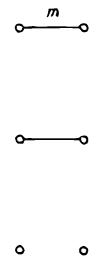
\includegraphics[keepaspectratio]{images/part001_5ff7a109.jpg}}

当 \(m = 3\) 时），而在

当 \(m = 2\) 时。*对称群 \(\mathfrak{S}_n\) 的 Coxeter 图表示为

\pandocbounded{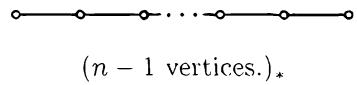
\includegraphics[keepaspectratio]{images/part001_1071b0ee.jpg}}

我们将在后面（第 V 章，第 4 节）证明，反过来，每个 Coxeter 矩阵都是某个 Coxeter 系统的矩阵。

如果 Coxeter 图的底图连通（附录，第 2 号）且非空，则称 Coxeter 系统 \((W,S)\) 是不可约的。等价地，S 非空，并且不存在将 S 划分为两个不同子集 \(S'\) 和 \(S''\) 的划分，使得 \(S'\) 的每个元素都与 \(S''\) 的每个元素交换。更一般地，设 \((\Gamma_{i})_{i\in I}\) 为 \(\Gamma\) 的连通分支族（附录，第 2 号），并设 \(S_{i}\) 为 \(\Gamma_{i}\) 的顶点集。令 \(W_{i}=W_{S_i}\) 为由 \(S_{i}\) 生成的 W 的子群（参见第 8 号）。于是 \((W_{i},S_{i})\) 是不可约 Coxeter 系统（第 8 号，定理 2），称为 \((W,S)\) 的不可约分支。此外，群 W 是限制直积 \(^{4}\)，其因子为子群 \(W_{i}\)（其中 \(i\in I\)）。事实上，这由下面更一般的命题得到：

命题 8. 设 \((\mathrm{S}_{i})_{i\in\mathrm{I}}\) 是 S 的一个划分，使得 \(S_{i}\) 的每个元素都与 \(S_{j}\) 的每个元素交换，只要 \(i\neq j\)。对于所有 \(i\in I\)，令 \(W_{i}\) 为由 \(S_{i}\) 生成的子群。于是 W 是族 \((\mathrm{W}_{i})_{i\in\mathrm{I}}\) 的限制直积。

显然，对于所有 \(i \in I\)，子群 \(W_i'\) 由 \(W_j\)（其中 \(j \neq i\)）的并生成，也由 \(S_i' = \bigcup_{i \neq j} S_j\) 生成。因此

\[
\mathrm{W} _ {i} \cap \mathrm{W} _ {i} ^ {\prime} = \mathrm{W} _ {\varnothing} = \{1 \}
\]

由第 8 号的定理 2。由于 W 由各 \(W_{i}\) 的并生成，命题得证。

\section{Tits 系统}

在本段中，字母 G、B、N、S、T、W 的含义如下文第 1 号所规定。

\subsection{定义与初步性质}

设 G 为一个群，B 为 G 的一个子群。群 \(B \times B\) 通过 \((b, b')\) . \(g = bgb'^{-1}\) 作用在 G 上，其中 \(b, b' \in B\) 且 \(g \in G\)。\(B \times B\) 在 G 上的轨道是当 \(g \in G\) 时的集合 BgB，称为关于 B 的 G 的双陪集。它们构成 G 的一个划分；相应的商记为 B\textbackslash G/B。若 C 和 C' 是双陪集，则 CC' 是双陪集的并。

定义 1. Tits 系统是一个四元组 \((\mathbf{G},\mathbf{B},\mathbf{N},\mathbf{S})\)，其中 \(\mathbf{G}\) 是一个群，\(\mathbf{B}\) 和 \(\mathbf{N}\) 是 \(\mathbf{G}\) 的两个子群，\(\mathbf{S}\) 是 \(\mathrm{N} / (\mathrm{B}\cap \mathrm{N})\) 的一个子集，并满足下列公理：

(T1) 集合 \(\mathrm{B} \cup \mathrm{N}\) 生成 \(\mathrm{G}\)，且 \(\mathrm{B} \cap \mathrm{N}\) 是 \(\mathrm{N}\) 的正规子群。

(T2) 集合 S 生成群 \(W = N/(B \cap N)\)，并且由阶为 2 的元素组成。

(T3) \(sBw \subset BwB \cup BswB\)，其中 \(s \in S\) 且 \(w \in W\)。

(T4) 对所有 \(s \in S\)，都有 \(sBs \not\subset B\)。

群 \(W = N / (B \cap N)\) 有时称为 Tits 系统 \((G, B, N, S)\) 的 Weyl 群。

备注。1) 我们将在第 5 号（定理 3 的推论）看到，如果给定 (G, B, N)，则至多存在一个 N/(B∩N) 的子集 S，使得 (G, B, N, S) 是 Tits 系统。

\begin{enumerate}
\def\labelenumi{\arabic{enumi})}
\setcounter{enumi}{1}
\tightlist
\item
  设 \((G, B, N, S)\) 是一个 Tits 系统，Z 是 G 的包含于 B 中的正规子群。令 \(G' = G/Z, B' = B/Z, N' = N/(Z \cap N)\)，并令 \(S'\) 为 S 在 \(N'/(B' \cap N')\) 中的像。立即可见，\((G', B', N', S')\) 是一个 Tits 系统。
\end{enumerate}

在本段中，设 \((\mathrm{G},\mathrm{B},\mathrm{N},\mathrm{S})\) 为一个 Tits 系统，并置 \(T=B\cap N\)、W=N/T。双陪集均指 G 关于 B 的双陪集。对于任意 \(w\in W\)，置 \(C(w)=BwB\)；这是一个双陪集。

我们将从公理 (T1) 至 (T4) 推出若干初等结论。用 \(w, w', \ldots\) 表示 W 的元素，用 \(s, s', \ldots\) 表示 S 的元素。以下关系是显然的：

\[
\mathrm{C} (1) = \mathrm{B}, \quad \mathrm{C} (w w ^ {\prime}) \subset \mathrm{C} (w). \mathrm{C} (w ^ {\prime}), \quad \mathrm{C} (w ^ {- 1}) = \mathrm{C} (w) ^ {- 1}.\tag{1}
\]

公理 (T3) 也可写成

\[
\mathrm{C} (s). \mathrm{C} (w) \subset \mathrm{C} (w) \cup \mathrm{C} (s w).\tag{2}
\]

此外，由 (1) 有 \(C(sw) \subset C(s).C(w)\)，又因 \(C(s).C(w)\) 是双陪集的并，故只有以下两种可能：

\[
\mathrm{C} (s). \mathrm{C} (w) = \left\{ \begin{array}{l l} \mathrm{C} (s w) & \text {if} \mathrm{C} (w) \not \subset \mathrm{C} (s). \mathrm{C} (w) \\ \mathrm{C} (w) \cup \mathrm{C} (s w) & \text {if} \mathrm{C} (w) \subset \mathrm{C} (s). \mathrm{C} (w). \end{array} \right.\tag{3}
\]

由 (T4)，\(\mathrm{B} \neq \mathrm{C}(s). \mathrm{C}(s)\)；在 (3) 中令 \(w = s\)，并利用关系 \(s^2 = 1\)，得到

\[
\mathrm{C} (s). \mathrm{C} (s) = \mathrm{B} \cup \mathrm{C} (s).\tag{4}
\]

此公式表明，\(B \cup C(s)\) 是 G 的一个子群。将 (4) 两边右乘 \(C(w)\)，并利用公式 (3) 以及关系

\[
\mathrm{B.C} (w) = \mathrm{C} (w),
\]

得到

\[
\mathrm{C} (s). \mathrm{C} (s). \mathrm{C} (w) = \mathrm{C} (w) \cup \mathrm{C} (s w).\tag{5}
\]

对公式 (2)、(3) 和 (5) 中出现的集合取逆，然后以 \(w^{-1}\) 代替 w，得到公式

\[
\mathrm{C} (w). \mathrm{C} (s) \subset \mathrm{C} (w) \cup \mathrm{C} (w s)\tag{(2')}
\]

\[
\mathrm{C} (w). \mathrm{C} (s) = \mathrm{C} (w s) \quad \text {   if   } \mathrm{C} (w) \not \subset \mathrm{C} (w). \mathrm{C} (s)
\]

\[
\mathrm{C} (w). \mathrm{C} (s) = \left\{ \begin{array}{l l} \mathrm{C} (w) \cup \mathrm{C} (w s) & \text {if} \mathrm{C} (w) \subset \mathrm{C} (w). \mathrm{C} (s) \end{array} \right.\tag{3'}
\]

\[
\mathrm{C} (w). \mathrm{C} (s). \mathrm{C} (s) = \mathrm{C} (w) \cup \mathrm{C} (w s).\tag{(5')}
\]

引理 1. 设 \(s_1, \ldots, s_q \in S\)，且 \(w \in W\)。我们有

\[
\mathrm{C} \left(s _ {1} \dots s _ {q}\right). \mathrm{C} (w) \subset \bigcup_ {\left(i _ {1}, \dots i _ {p}\right)} \mathrm{C} \left(s _ {i _ {1}} \dots s _ {i _ {p}} w\right),
\]

其中，\((i_1, \ldots, i_p)\) 表示区间 \([1, q]\) 中严格递增的整数序列的集合。

我们对 \(q\) 作归纳证明，\(q = 0\) 的情形是平凡的。当 \(q \geqslant 1\) 时，有 \(C(s_1 \ldots s_q).C(w) \subset C(s_1).C(s_2 \ldots s_q).C(w)\)。由归纳假设，\(C(s_2 \ldots s_q).C(w)\) 包含于各个 \(C(s_{j_1} \ldots s_{j_p}w)\) 的并中，其中

\[
2 \leqslant j _ {1} <   \dots <   j _ {p} \leqslant q.
\]

由 (T3)，集合 \(C(s_{1}).C(s_{j_{1}}\ldots s_{j_{p}}w)\) 包含于集合 \(C(s_{1}s_{j_{1}}\ldots s_{j_{p}}w)\) 与 \(C(s_{j_{1}}\ldots s_{j_{p}}w)\) 的并中。这就证明了引理。

\subsection{一个例子}

设 \(k\) 为一个域，\(n\) 为一个 \(\geqslant 0\) 的整数，且 \((e_i)\) 为 \(k^n\) 的标准基。令 \(G = GL(n, k)\)，令 \(B\) 为 \(G\) 的上三角子群，令 \(N\) 为 \(G\) 的由每行每列恰有一个非零元素的矩阵组成的子群。\(N\) 中的一个元素置换直线 \(ke_i\)；这给出一个满同态 \(N \to \mathfrak{S}_n\)，其核是对角矩阵组成的子群 \(T = B \cap N\)，并允许我们将 \(W = N/T\) 与 \(\mathfrak{S}_n\) 认同。记 \(s_j\)（\(1 \leqslant j \leqslant n - 1\)）为 \(W\) 中对应于 \(j\) 与 \(j + 1\) 的换位的元素；令 \(S\) 为 \(s_j\) 的集合。四元组 \((G, B, N, S)\) 是一个 Tits 系统。事实上：

公理 (T1) 由《代数》第 II 章第 10 节第 13 号命题 2 的推论得出。

公理 (T2) 在《代数》第 I 章第 97 页的勘误中得到证明。

公理 (T4) 是立即的。

还需验证公理 (T3)，即

\[
s _ {j} \mathrm{B} w \subset \mathrm{B} w \mathrm{B} \cup \mathrm{B} s _ {j} w \mathrm{B} \quad \text { for } 1 \leqslant j \leqslant n - 1, w \in \mathrm{W},
\]

或等价地，

\[
s _ {j} \mathrm{B} \subset \mathrm{BB} ^ {\prime} \cup \mathrm{Bs} _ {j} \mathrm{B} ^ {\prime}, \quad \text { with } \mathrm{B} ^ {\prime} = w \mathrm{B} w ^ {- 1}.
\]

令 \(G_{j}\) 为 G 的如下子群：其中的元素固定所有 \(e_{i}\)（对于 \(i \neq j, j + 1\)），并保持由 \(e_{j}\) 和 \(e_{j+1}\) 张成的平面；该群同构于 \(\mathbf{GL}(2, k)\)。容易验证 \(G_{j}B = BG_{j}\)。由于 \(s_{j} \in G_{j}\)，有 \(s_{j}B \subset BG_{j}\)，因此只需证明

\[
\mathrm{G} _ {j} \subset (\mathrm{B} \cap \mathrm{G} _ {j}) (\mathrm{B} ^ {\prime} \cap \mathrm{G} _ {j}) \cup (\mathrm{B} \cap \mathrm{G} _ {j}) s _ {j} (\mathrm{B} ^ {\prime} \cap \mathrm{G} _ {j}).
\]

将 \(G_{j}\) 与 \(\mathbf{GL}(2,k)\) 认同；此时群 \(B \cap G_{j}\) 认同于上三角子群 \(B_{2}\)（属于 \(\mathbf{GL}(2,k)\)），而群 \(B' \cap G_{j}\) 在第一种情形下认同于 \(\mathbf{B}_2\)，其中 \(w(j) < w(j + 1)\)，在其他情形下认同于下三角子群 \(\mathbf{B}_2^-\)。在第一种情形下，要证明的公式可写成

\[
\mathbf {G L} (2, k) = \mathrm{B} _ {2} \cup \mathrm{B} _ {2} s \mathrm{B} _ {2} \quad \text { where } \quad s = \left( \begin{array}{c c} 0 & 1 \\ 1 & 0 \end{array} \right);
\]

例如，这由以下事实得出：\(B_{2}\) 是 \(\mathbf{GL}(2,k)\) 作用于射影直线 \(\mathbf{P}_{1}(k)\) 时某一点的稳定子，并且在该点的补集上传递作用。在第二种情形下，要证明的公式可写成

\[
\mathbf {G L} (2, k) = \mathrm{B} _ {2} \mathrm{B} _ {2} ^ {-} \cup \mathrm{B} _ {2} s \mathrm{B} _ {2} ^ {-};
\]

由于 \(B_{2}^{-} = sB_{2}s\)，将前一个公式右乘 s 即得此结论。

\subsection{G 分解为双陪集}

定理 1. 有 G = BWB。映射 \(w \mapsto C(w)\) 是从 W 到关于 B 的 G 的双陪集集合 B\textbackslash G/B 的一个双射。

显然，BWB 在映射 \(x \mapsto x^{-1}\) 下不变，而引理 1 表明它在乘法下不变。由于它包含 B 和 N，故等于 G。

还需证明 \(\mathrm{C}(w) \neq \mathrm{C}(w')\)，当 \(w \neq w'\) 时。为此，我们将对整数 \(q\) 作归纳，证明以下断言：

(Aq) 若 w 和 \(w'\) 是 W 中满足 \(l_{S}(w) \geqslant l_{S}(w') = q\) 的不同元素，则 \(C(w) \neq C(w')\)。

（关于 \(l_{\mathbb{S}}(w)\) 的定义，见 §1，第 1 号。）

当 \(q = 0\) 时此断言显然，因为此时 \(w' = 1\) 且 \(w \neq 1\)，所以 \(C(w') = B\) 而 \(C(w) \neq B\)。

假设 \(q \geqslant 1\)，且 \(w, w'\) 满足 \((\mathbf{A}_q)\) 的假设。存在 \(s \in S\)，使得 \(sw'\) 的长度为 \(q - 1\)。我们有

\[
l _ {S} (w) > l _ {S} \left(s w ^ {\prime}\right)\tag{6}
\]

因此 \(w \neq sw'\)。此外，\(sw \neq sw'\)；由第 1 节第 1 号的公式 (3)，有

\[
l _ {\mathrm{S}} (s w) \geqslant l _ {\mathrm{S}} (w) - 1 \geqslant l _ {\mathrm{S}} (s w ^ {\prime}) = q - 1.\tag{7}
\]

由归纳假设，\(C(sw')\) 与 \(C(w)\) 及 \(C(sw)\) 均不相同；由公式 (2) 得

\[
\mathrm{C} (s w ^ {\prime}) \cap \mathrm{C} (s). \mathrm{C} (w) = \varnothing .\tag{8}
\]

由于 \(\mathrm{C}(sw') \subset \mathrm{C}(s).\mathrm{C}(w')\)，最后得到 \(\mathrm{C}(w) \neq \mathrm{C}(w')\)。

备注。上述证明没有使用公理 (T4)。

\subsection{与 Coxeter 系统的关系}

定理 2. \((\mathrm{W},\mathrm{S})\) 是一个 Coxeter 系统。此外，对于 \(s\in \mathrm{S}\) 和 \(w\in \mathrm{W}\)，关系 \(\mathrm{C}(sw) = \mathrm{C}(s).C(w)\) 与 \(l_{\mathbb{S}}(sw) > l_{\mathbb{S}}(w)\) 等价。

对于任意 \(s \in S\)，令 \(P_s\) 为元素 \(w \in W\) 的集合，满足

\[
\mathrm{C} (s). \mathrm{C} (w) = \mathrm{C} (s w).
\]

我们将验证 \(P_{s}\) 满足第 1 节第 7 号的条件 (\(A'\))、(\(B'\)) 和 (C)；然后定理的两个断言将由第 1 节第 7 号的命题 6 得出。

条件 \((\mathbf{A}^{\prime})\) 是显然的。

我们验证 (B')。若 \(P_{s}\) 和 \(sP_{s}\) 有公共元素 w，则有 \(w \in P_{s}\) 和 \(sw \in P_{s}\)，从而

\[
\mathrm{C} (s). \mathrm{C} (w) = \mathrm{C} (s w), \quad \mathrm{C} (s). \mathrm{C} (s w) = \mathrm{C} (w).
\]

于是 \(\mathrm{C}(s).\mathrm{C}(s).\mathrm{C}(w) = \mathrm{C}(w)\)，并且由公式 (5) 可知 \(\mathrm{C}(w) = \mathrm{C}(sw)\)，这与定理 1 矛盾。

我们验证 (C)。设 \(s, s' \in S\)，且 \(w, w' \in W\) 满足 \(w' = ws'\)。假设 \(w \in P_s\) 而 \(w' \notin P_s\)，则

\[
\mathrm{C} (s w) = \mathrm{C} (s). \mathrm{C} (w)\tag{9}
\]

\[
\mathrm{C} (w ^ {\prime}) \subset \mathrm{C} (s). \mathrm{C} (w ^ {\prime})\tag{10}
\]

由 (3) 得。

由 (9) 以及关系 \(w = w's'\)，得到

\[
\mathrm{C} (s) w ^ {\prime} s ^ {\prime} \mathrm{B} = \mathrm{C} (s w).\tag{11}
\]

由公式 \((2')\)，有 \(C(w')\)。\(C(s') \subset C(w') \cup C(w's')\)，立即推出

\[
\mathrm{C} (w ^ {\prime}) s ^ {\prime} \mathrm{B} \subset \mathrm{C} (w s ^ {\prime}) \cup \mathrm{C} (w).\tag{12}
\]

由于 \(C(w')\) 是左陪集 gB 的并，且

\[
\mathrm{C} (s). \mathrm{C} (w ^ {\prime}) = \mathrm{C} (s) w ^ {\prime} \mathrm{B},
\]

公式 (10) 表明 \(C(s)w'\) 与 \(C(w')\) 相交，从而当然 \(C(s)w's'B\) 与 \(C(w')s'B\) 相交。由公式 (11) 和 (12) 可知，双陪集 \(C(sw)\) 等于双陪集 \(C(ws')\) 和 \(C(w)\) 中的一个；由于 \(sw \neq w\)，由定理 1 可得 \(sw = ws'\)。

推论 1. 设 \(w_{1}, \ldots, w_{q} \in \mathbf{W}\)，并令 \(w = w_{1} \ldots w_{q}\)。若

\[
l _ {S} (w) = l _ {S} \left(w _ {1}\right) + \dots + l _ {S} \left(w _ {q}\right),
\]

则

\[
\mathrm{C} (w) = \mathrm{C} (w _ {1}) \dots \mathrm{C} (w _ {q}).
\]

取各 \(w_{i}\) 的约化分解后，问题归结为约化分解的情形

\[
w = s _ {1} \dots s _ {q}, \quad \text { with } s _ {i} \in S.
\]

若 \(u = s_2 \ldots s_q\)，则 \(w = s_1u\)，且 \(l_{\mathbb{S}}(s_1u) > l_{\mathbb{S}}(u)\)，所以由定理有 \(\mathrm{C}(w) = \mathrm{C}(s_1). \mathrm{C}(u)\)。对 \(q\) 作归纳，即得所需公式。

推论 2. 设 \(w \in W\)，令 \(T_w\) 为 \(W\) 的子集，按照第 1 节第 4 号的引理 2 与 \(w\) 相关联。若 \(t \in T_w\)，则

\[
\mathrm{C} (t) \subset \mathrm{C} (w). \mathrm{C} (w ^ {- 1}).
\]

若 \(t \in \mathrm{T}_w\)，则按定义，存在 \(w', w'' \in \mathrm{W}\) 和 \(s \in \mathrm{S}\)，使得

\[
w = w ^ {\prime} s w ^ {\prime \prime}, l _ {S} (w) = l _ {S} (w ^ {\prime}) + l _ {S} (w ^ {\prime \prime}) + 1 \quad \text {and} \quad t = w ^ {\prime} s w ^ {\prime - 1}.
\]

由推论 1，

\[
\mathrm{C} (w). \mathrm{C} (w ^ {- 1}) = \mathrm{C} (w ^ {\prime}). \mathrm{C} (s). \mathrm{C} (w ^ {\prime \prime}). \mathrm{C} (w ^ {\prime \prime - 1}). \mathrm{C} (s). \mathrm{C} (w ^ {\prime - 1}).
\]

因此，

\[
\mathrm{C} (w). \mathrm{C} (w ^ {- 1}) \supset \mathrm{C} (w ^ {\prime}). \mathrm{C} (s). \mathrm{C} (s). \mathrm{C} (w ^ {\prime - 1}).
\]

由 (4)，\(\mathrm{C}(s) \subset \mathrm{C}(s). \mathrm{C}(s)\)。因此，

\[
\mathrm{C} (w). \mathrm{C} (w ^ {- 1}) \supset \mathrm{C} (w ^ {\prime}). \mathrm{C} (s). \mathrm{C} (w ^ {\prime - 1}) \supset \mathrm{C} (t).
\]

推论 3. 设 \(w \in W\)，令 \(H_w\) 为 \(G\) 的子群，由 \(C(w).C(w^{-1})\) 生成。则：

\begin{enumerate}
\def\labelenumi{\alph{enumi})}
\tightlist
\item
  对任意约化分解 \((s_1,\ldots ,s_q)\) 的 \(w\)，
\end{enumerate}

\[
\mathrm{C} (s _ {j}) \subset \mathrm{H} _ {w} \quad \text { for } 1 \leqslant j \leqslant q.
\]

\begin{enumerate}
\def\labelenumi{\alph{enumi})}
\setcounter{enumi}{1}
\tightlist
\item
  群 \(\mathrm{H}_w\) 包含 \(\mathrm{C}(w)\)，且由 \(\mathrm{C}(w)\) 生成。
\end{enumerate}

我们对 \(a)\) 作关于 \(j\) 的归纳证明。假设 \(C(s_k)\) 包含于 \(H_w\)，其中 \(k < j\)。令

\[
t = (s _ {1} \dots s _ {j - 1}) s _ {j} (s _ {1} \dots s _ {j - 1}) ^ {- 1}.
\]

元素 \(t\) 属于定义于第 1 节第 4 号的引理 2 中的子集 \(\mathrm{T}_w\)，它是 \(\mathbf{W}\) 的子集。由推论 2，\(\mathrm{C}(t) \subset \mathrm{H}_w\)，从而 \(\mathrm{C}(s_j) \subset \mathrm{H}_w\)。

由于 \(\mathrm{C}(w) = \mathrm{C}(s_1) \ldots \mathrm{C}(s_q)\)，参见推论 1，故 \(\mathrm{C}(w) \subset \mathrm{H}_w\)，于是得到 \(b)\)。

例。将定理 2 应用于第 2 号所述的 Tits 系统，可知对称群 \(S_{n}\) 以及相邻元素的换位集合构成一个 Coxeter 群。

\subsection{包含 B 的 G 的子群}

对于任意子集 \(X\)，它是 \(S\) 的子集，我们将 \(W_X\) 记作 \(W\) 中由 \(X\) 生成的子群，并将 \(G_X\) 记作 \(BW_X B\) 中的双陪集 \(C(w)\)（其中 \(w \in W_X\)）的并集。我们有 \(G_\varnothing = B\) 且 \(G_S = G\)。

定理 3. a) 对于任意子集 \(X\)（\(S\) 的子集），集合 \(G_X\) 是 \(G\) 的一个子群，由 \(\bigcup_{s \in X} C(s)\) 生成。

\begin{enumerate}
\def\labelenumi{\alph{enumi})}
\setcounter{enumi}{1}
\item
  映射 \(\mathrm{X} \mapsto \mathrm{G}_{\mathrm{X}}\) 是从 \(\mathfrak{P}(\mathrm{S})\) 到 \(\mathrm{G}\) 的包含 \(\mathrm{B}\) 的子群集合的一个双射。
\item
  设 \((\mathrm{X}_i)_{i\in I}\) 是 X 的子集族。若 \(X = \bigcap_{i\in I}X_i\)，则 \(G_X = \bigcap_{i\in I}G_{X_i}\)。
\item
  设 X 和 Y 是 S 的两个子集。则 \(G_{X} \subset G_{Y}\)（分别为 \(G_{X} = G_{Y}\)）当且仅当 \(X \subset Y\)（分别为 X = Y）。
\end{enumerate}

显然 \(G_{X} = (G_{X})^{-1}\)；第 1 号的引理 1 表明 \(G_{X}.G_{X} \subset G_{X}\)；因此，考虑到定理 2 的推论 1，\(a)\) 得证。

映射 \(\mathrm{X} \mapsto \mathrm{G}_{\mathrm{X}}\) 的单射性由映射 \(\mathrm{X} \mapsto \mathrm{W}_{\mathrm{X}}\) 的单射性推出（参见~§1，第 8 号，定理 2）。反过来，设 \(\mathrm{H}\) 是 \(\mathrm{G}\) 的一个包含 \(\mathrm{B}\) 的子群。令 \(\mathrm{U}\) 为 \(w \in \mathrm{W}\) 且 \(C(w) \subset \mathrm{H}\) 的集合。我们有 \(\mathrm{H} = \mathrm{BUB}\)，因为 \(\mathrm{H}\) 是双陪集的并。令 \(\mathrm{X} = \mathrm{U} \cap \mathrm{S}\)；我们证明 \(\mathrm{H} = \mathrm{G}_{\mathrm{X}}\)。显然，\(\mathrm{G}_{\mathrm{X}} \subset \mathrm{H}\)。另一方面，令 \(u \in \mathrm{U}\)，并令 \((s_1, \ldots, s_q)\) 是 \(u\) 的一个约化分解。定理 2 的推论 3 蕴含 \(C(s_j) \subset \mathrm{H}\)，从而 \(s_j \in \mathrm{X}\)，其中 \(1 \leqslant j \leqslant q\)。因此，\(u \in \mathrm{W}_{\mathrm{X}}\)，且由于 \(\mathrm{H}\) 是各个 \(C(u)\) 的并（其中 \(u \in \mathrm{U}\)），我们有 \(\mathrm{H} \subset \mathrm{G}_{\mathrm{X}}\)，这就证明了 \(b\)。

断言 \(c)\) 和 \(d)\) 由 \(W_X\) 的相应性质推出（\(\S 1\)，第 8 号，定理 2）。

推论。集合 \(S\) 由这样的元素 \(w \in W\) 组成：\(w \neq 1\) 且 \(B \cup C(w)\) 是 \(G\) 的一个子群。

满足 \(w \in W\) 且 \(B \cup C(w)\) 是 G 的子群的元素，正是存在 \(X \subset S\) 使得 \(W_{X} = \{1, w\}\) 的那些元素。此外，若 \(w \neq 1\)，则必有 \(\text{Card}(X) = 1\)，即 \(w \in S\)。

备注。1) 上述推论表明，S 由 (G, B, N) 决定；因此，我们有时也允许自己说 (G, B, N) 是一个 Tits 系统，或 (B, N) 是 G 中的一个 Tits 系统。

命题 1. 设 X 是 S 的一个子集，N' 是 N 的一个子群，其在 W 中的像等于 W\_X。则，(G\_X, B, N', X) 是一个 Tits 系统。

我们有 \(G_{X} = BW_{X}B = BN'B\)，这表明 \(G_{X}\) 由 \(B \cup N'\) 生成。现在验证公理 (T1) 至 (T4) 是直接的。

命题 2. 设 \(\mathrm{X}, \mathrm{Y} \subset \mathrm{S}\) 且 \(w \in \mathrm{W}\)。我们有

\[
\mathrm{G} _ {\mathrm{X}} w \mathrm{G} _ {\mathrm{Y}} = \mathrm{BW} _ {\mathrm{X}} w \mathrm{W} _ {\mathrm{Y}} \mathrm{B}.
\]

令 \(s_1, \ldots, s_q \in X\) 且 \(t_1, \ldots, t_q \in Y\)。引理 1 表明

\[
\mathrm{C} (s _ {1} \dots s _ {q}). \mathrm{C} (w). \mathrm{C} (t _ {1} \dots t _ {q}) \subset \mathrm{BW} _ {\mathrm{X}} w \mathrm{W} _ {\mathrm{Y}} \mathrm{B},
\]

从而

\[
\mathrm{G} _ {\mathrm{X}} w \mathrm{G} _ {\mathrm{Y}} \subset \mathrm{BW} _ {\mathrm{X}} w \mathrm{W} _ {\mathrm{Y}} \mathrm{B}.
\]

反向包含关系显然成立。

备注。2) 记 \(G_X \backslash G / G_Y\) 为 \(G\) 中形如 \(G_X gG_Y\)（其中 \(g \in G\)）的子集的集合；并类似地定义 \(W_X \backslash W / W_Y\)。前一命题表明，典范双射 \(w \mapsto C(w)\)，从 \(W\) 到 \(B \backslash G / B\)，通过取商定义了一个双射 \(W_X \backslash W / W_Y \to G_X \backslash G / G_Y\)。

命题 3. 设 \(\mathbf{X} \subset \mathbf{S}\) 且 \(g \in \mathbf{G}\)。关系 \(g\mathrm{B}g^{-1} \subset \mathbf{G}_{\mathbf{X}}\) 蕴含 \(g \in \mathbf{G}_{\mathbf{X}}\)。

设 \(w \in W\) 使得 \(g \in C(w)\)。由于 B 是 \(G_X\) 的一个子群，假设 \(gBg^{-1} \subset G_X\) 蕴含 \(C(w).C(w^{-1}) \subset G_X\)，进而由定理 2 的推论 3 得 \(C(w) \subset G_X\)，所以 g 属于 \(G_X\)。

\subsection{抛物子群}

定义 2. 若 G 的一个子群包含 B 的某个共轭子群，则称其为抛物子群。

显然，每个包含一个抛物子群的子群都是抛物子群。

命题 4. 设 P 是 G 的一个子群。

\begin{enumerate}
\def\labelenumi{\alph{enumi})}
\item
  P 是抛物子群，当且仅当存在 S 的一个子集 X，使得 P 与 \(G_{X}\) 共轭（关于 \(G_{X}\) 的定义见~第 5 号）。
\item
  设 \(\mathrm{X}, \mathrm{X}' \subset \mathrm{S}\) 且 \(g, g' \in \mathrm{G}\) 满足 \(\mathrm{P} = g\mathrm{G}_{\mathrm{X}}g^{-1} = g'\mathrm{G}_{\mathrm{X}'}g'^{-1}\)。则 \(\mathrm{X} = \mathrm{X}'\) 且 \(g'g^{-1} \in \mathrm{P}\)。
\end{enumerate}

断言 a) 由定理 3 b) 得出。

在 \(b\) 的假设下，有

\[
g ^ {- 1} g ^ {\prime} \mathrm{B} g ^ {\prime - 1} g \subset g ^ {- 1} g ^ {\prime} \mathrm{G} _ {\mathrm{X} ^ {\prime}} g ^ {\prime - 1} g = \mathrm{G} _ {\mathrm{X}},
\]

且命题 3 表明 \(g^{-1}g' \in \mathrm{G}_X\)。因此，\(\mathrm{G}_{\mathrm{X}'} = \mathrm{G}_X\) 且 \(\mathrm{X}' = \mathrm{X}\)，由定理 3 b)。最后，

\[
g ^ {\prime} g ^ {- 1} = g. g ^ {- 1} g ^ {\prime}. g ^ {- 1} \in g \mathrm{G} _ {\mathrm{X}} g ^ {- 1},
\]

这就证明了 b)。

若抛物子群 P 与 \(G_{X}\) 共轭，其中 \(X \subset S\)，则称 P 为 X 型。

定理 4. (i) 设 \(\mathbf{P}_1\) 和 \(\mathbf{P}_2\) 是 \(\mathbf{G}\) 的两个抛物子群，且其交为抛物子群；设 \(g \in \mathbf{G}\) 满足 \(g\mathrm{P}_1g^{-1} \subset \mathrm{P}_2\)。则 \(g \in \mathbf{P}_2\) 且 \(\mathbf{P}_1 \subset \mathbf{P}_2\)。

\begin{enumerate}
\def\labelenumi{(\roman{enumi})}
\setcounter{enumi}{1}
\item
  交为抛物子群的两个抛物子群不共轭。
\item
  设 \(\mathbf{Q}_1\) 和 \(\mathbf{Q}_2\) 是 \(\mathbf{G}\) 的两个抛物子群，包含于子群 \(\mathbf{Q}\) 中，而该群是 \(\mathbf{G}\) 的子群。则任意 \(g \in \mathbf{G}\)，若满足 \(g\mathbf{Q}_1g^{-1} = \mathbf{Q}_2\)，就属于 \(\mathbf{Q}\)。
\item
  每个抛物子群都是自身的规范化子 \(^{6}\)。
\end{enumerate}

断言 (i) 由命题 3 和 4 得出，并蕴含 (ii)。在 (iii) 的假设下，有 \(gQ_{1}g^{-1} \subset Q\)，由 (i) 得 \(g \in Q\)。最后，(iv) 由 (iii) 取 \(Q_{1} = Q_{2} = Q\) 得出。

命题 5. 设 \(\mathbf{P}_1\) 和 \(\mathbf{P}_2\) 是 \(\mathbf{G}\) 的两个抛物子群。则 \(\mathbf{P}_1 \cap \mathbf{P}_2\) 包含 \(\mathbf{T}\) 的某个共轭子群。

先用 G 的一个内自同构变换 \(P_{1}\) 和 \(P_{2}\)，可假定 \(B \subset P_{1}\)。设 \(g \in G\) 满足 \(gBg^{-1} \subset P_{2}\)。由定理 1，存在 \(n \in N\) 和 \(b, b' \in B\)，使得 \(g = bnb'\)。由于 T 在 N 中正规，

\[
\mathrm{P} _ {2} \supset g \mathrm{B} g ^ {- 1} = b n \mathrm{B} n ^ {- 1} b ^ {- 1} \supset b n \mathrm{T} n ^ {- 1} b ^ {- 1} = b \mathrm{T} b ^ {- 1}
\]

并且

\[
\mathrm{P} _ {1} \supset \mathrm{B} \supset b \mathrm{T} b ^ {- 1},
\]

这就证明了命题。

\subsection{简单性定理}

引理 2. 设 H 是 G 的一个正规子群。存在 S 的一个子集 X，使得 BH = G\_X，并且 X 的每个元素都与 S-X 的每个元素交换。

由于 BH 是包含 B 的 G 的一个子群，定理 3 给出 S 的唯一子集 X，使得 \(BH = G_{X}\)。

设 \(s_1 \in X\) 且 \(s_2 \in S - X\)；设 \(n_1\) 和 \(n_2\) 分别是 \(N\) 中 \(s_1\) 和 \(s_2\) 的代表元。于是 \(n_1 \in G_X = BH\)，存在 \(b \in B\) 使得 \(bn_1 \in H\)。由于 \(H\) 是 \(G\) 的正规子群，元素 \(h = n_2bn_1n_2^{-1}\) 属于 \(G\)，且属于 \(H\)。这意味着

\[
h \in \mathrm{C} (s _ {2}). \mathrm{C} (s _ {1}). \mathrm{C} (s _ {2}).
\]

若 \(s_2s_1s_2\) 的长度等于 3，则定理 2 的推论 1 表明

\[
\mathrm{C} (s _ {2}). \mathrm{C} (s _ {1}). \mathrm{C} (s _ {2}) = \mathrm{C} (s _ {2} s _ {1} s _ {2}),
\]

从而 \(h \in H \cap C(s_{2}s_{1}s_{2})\)。由于 \(H \cap C(s_{2}s_{1}s_{2})\) 非空，\(s_{2}s_{1}s_{2} \in W_{X}\)。又因 \((s_{2}, s_{1}, s_{2})\) 是一个约化分解，故 \(s_{2} \in X\)，这与我们的假设矛盾。

因此 \(l_{\mathrm{S}}(s_2s_1s_2) \leqslant 2\)；若 \(l_{\mathrm{S}}(s_2s_1s_2) = 1\)，则 \(s_1s_2 \in \mathrm{S}\)，从而 \((s_1s_2)^2 = 1\)，或者 \(s_1s_2 = s_2s_1\)。若 \(l_{\mathrm{S}}(s_2s_1s_2) = 2\)，则第 1 节第 5 号的性质 (E) 蕴含 \(s_2s_1 = s_1s_2\)，因为 \(s_1 \neq s_2\)。证毕。

下面的群 U 的性质将在下文定理 5 中用到：

\begin{enumerate}
\def\labelenumi{(\Alph{enumi})}
\setcounter{enumi}{17}
\tightlist
\item
  对于 U 的任意不同于 U 的正规子群 V，U/V 的换位子群（参见《代数》第 I 章第 6 节第 8 号）不同于 U/V。
\end{enumerate}

每个可解群都满足 (R)；特别地，每个阿贝尔群都满足 (R)。可以证明，对称群 \(S_{n}\) 满足 (R)（参见习题 29）。

定理 5. 设 Z 为 B 的所有共轭子群的交，U 为 B 的一个子群，且 \(G_{1}\) 为 G 中由 U 的共轭子群生成的子群。作如下假设：

\begin{enumerate}
\def\labelenumi{\arabic{enumi})}
\item
  U 在 B 中正规且 B = UT。
\item
  U 具有性质 (R.)。
\item
  \(\mathbf{G}_1\) 等于其换位子群。
\item
  Coxeter 系统 (W, S) 是不可约的（参见~§ 1，第 9 号）。
\end{enumerate}

于是，G 中每个由 \(G_{1}\) 规范化的子群 H，或者包含于 Z，或者包含 \(G_{1}\)。

首先证明 \(G = G_{1}T\)。群 \(G_{1}T\) 包含 B，因而是自身的规范化子（定理 4）；但是由于 N 规范化 \(G_{1}\) 和 T，它也规范化 \(G_{1}T\)，故 \(N \subset G_{1}T\)。由于 G 由 B 和 N 生成，得到 \(G = G_{1}T\)。

接下来，置

\[
\begin{array}{c} \mathrm{G} ^ {\prime} = \mathrm{G} _ {1} \mathrm{H}, \quad \mathrm{B} ^ {\prime} = \mathrm{B} \cap \mathrm{G} ^ {\prime}, \quad \mathrm{N} ^ {\prime} = \mathrm{N} \cap \mathrm{G} ^ {\prime}, \\ \mathrm{T} ^ {\prime} = \mathrm{T} \cap \mathrm{G} ^ {\prime} = \mathrm{B} ^ {\prime} \cap \mathrm{N} ^ {\prime} \quad \text {and} \quad \mathrm{W} ^ {\prime} = \mathrm{N} ^ {\prime} / \mathrm{T} ^ {\prime}. \end{array}
\]

我们有 \(G = G'T\)，因为 \(G'\) 包含 \(G_{1}\)，因而 \(N = N'T\)。于是，\(N'\) 包含于 N 的嵌入通过取商定义了一个同构 \(\alpha : W' \to W\)。置 \(S' = \alpha^{-1}(S)\)。

现在证明 \((\mathrm{G}^{\prime},\mathrm{B}^{\prime},\mathrm{N}^{\prime},\mathrm{S}^{\prime})\) 是一个 Tits 系统。由于 G = BNB 且 B = TU = UT，有 G = UNU。由于 U 是 \(G^{\prime}\) 的一个子群，故 \(G^{\prime} = UN^{\prime}U\)；由于 \(U \subset B^{\prime}\)，这就证明了 (T1)。公理 (T2) 成立，因为 \(\alpha\) 是一个同构。设 \(w \in W\)，并令 \(w' = \alpha^{-1}(w)\) 为 \(W^{\prime}\) 中的相应元素。我们有

\[
\mathrm{B} w \mathrm{B} = \mathrm{B} w \mathrm{B} ^ {\prime} = \mathrm{B} w ^ {\prime} \mathrm{B} ^ {\prime}, \quad \text { since } \mathrm{B} = \mathrm{B} ^ {\prime} \mathrm{T}.
\]

由此得到 \(G' \cap BwB = B'w'B'\)，这意味着，\(G'\) 到 G 中的包含映射通过取商定义了一个从

\(B'\backslash G'/B'\) 到 \(B\backslash G/B\) 的双射。公理 (T3) 立即成立。公理 (T4) 由 \(B = B'T\) 得出。

子群 H 在 \(G'\) 中正规。将引理 2 应用于 \((G', B', N', S')\)，存在一个子集 \(X'\)，它是 \(S'\) 的子集，使得 \(B'H = G_{X'}'\)，且 \(S' - X'\) 的每个元素都与 \(X'\) 的每个元素交换。根据假设 (4)，只有两种可能：

\begin{enumerate}
\def\labelenumi{\alph{enumi})}
\item
  \(X' = \varnothing\)，即~\(B'H = B'\)，所以 \(H \subset B' \subset B\)。若 \(g \in G\)，则 \(g = g_1 t\)，其中 \(g_1 \in G_1\)、\(t \in T\)，且 \(H \subset g_1 Bg_1^{-1}\)，因为 \(G_1\) 规范化 \(H\)。因此 \(H \subset gBg^{-1}\)，并且由于 \(Z\) 是各个 \(gBg^{-1}\) 的交，我们有 \(H \subset Z\)。
\item
  \(X' = S'\)，即~\(B'H = G'\)。由于 \(G = G'T\)，我们有
\end{enumerate}

\[
\mathrm{G} = \mathrm{B} ^ {\prime} \mathrm{HT} = \mathrm{HB} ^ {\prime} \mathrm{T} = \mathrm{HB}.
\]

由于 B 规范化 U，U 的每个共轭子群都形如 \(hUh^{-1}\)，其中 \(h \in H\)。这样的子群包含于 UH 中，因而有 \(G_{1} \subset UH\)，根据 \(G_{1}\) 的定义。于是，我们有如下同构：

\[
\mathrm{U} / (\mathrm{U} \cap \mathrm{H}) \cong \mathrm{UH} / \mathrm{H} = \mathrm{G} _ {1} \mathrm{H} / \mathrm{H} \cong \mathrm{G} _ {1} / (\mathrm{G} _ {1} \cap \mathrm{H}).
\]

根据假设 (3)，\(G_{1}/(G_{1} \cap H)\) 等于其换位子群。假设 (2) 现在表明，群 \(U/(U \cap H)\)（它同构于 \(G_{1}/(G_{1} \cap H)\)）退化为单位元。因此 \(G_{1} \cap H = G_{1}\) 且 \(G_{1} \subset H\)，这就完成了证明。

推论。在定理 5 的假设下，群 \(\mathrm{G}_{1}/(\mathrm{G}_{1} \cap \mathrm{Z})\) 或者是非阿贝尔单群，或者退化为单位元。

定理 5 表明，\(G_{1}/(G_{1} \cap Z)\) 是单群或退化为单位元。另一方面，假设 (3) 蕴含它等于其换位子群。因此推论得证。

备注。1) 证明 \((\mathbf{G}', \mathbf{B}', \mathbf{N}', \mathbf{S}')\) 是一个 Tits 系统时，并未使用假设 (2)、(3)、(4)。

\begin{enumerate}
\def\labelenumi{\arabic{enumi})}
\setcounter{enumi}{1}
\item
  假设 \(\mathbf{Z} \cap \mathbf{U} = \{1\}\)。由于 \(\mathbf{Z}\) 和 \(\mathbf{U}\) 在 \(\mathbf{B}\) 中正规，故 \(\mathbf{Z}\) 的每个元素都与 \(\mathbf{U}\) 的每个元素交换，因而也与 \(\mathbf{G}_1\) 的每个元素交换。根据前一推论，\(\mathbf{G}_1 \cap \mathbf{Z}\) 是 \(\mathbf{G}_1\) 的中心。
\item
  假设 (3) 由下述条件蕴含：
\end{enumerate}

(3') U 由换位子 \(b^{-1}u^{-1}bu\) 生成，其中 \(u \in \mathbf{U}\) 且 \(b \in \mathbf{B} \cap \mathbf{G}_1\)。

例子。1) 设 \(k\) 是一个域，\(n\) 是满足 \(\geqslant 0\) 的整数，\(G = \mathbf{GL}(n, k)\)，并设 \((G, B, N, S)\) 是第 2 号中描述的 Tits 系统。令 \(U\) 为 \(G\) 的严格上三角子群，即 \(B\) 中由对角线元素等于 1 的矩阵组成的子群。定理 5 中的条件 (1) 是直接的，条件 (2) 也直接成立，因为 U 是可解的。当 \(n \geqslant 2\) 时，条件 (4) 得到满足。可以证明（参见~《代数》第 II 章第 10 节习题 13），当 \(n \geqslant 3\) 且 \(\operatorname{Card}(k) \geqslant 4\) 时，条件 (3) 得到满足。在这些条件下，我们得到 \(G_{1}/(G_{1} \cap Z)\) 是单群，并且 \(G_{1} \cap Z\) 是 \(G_{1}\) 的中心（参见~备注 2）。

当 \(k\) 为交换域时，\(G_1 = \mathbf{SL}(n,k)\)（参见~《代数》第 III 章第 8 节第 9 号）。

*2) 设 \(\mathfrak{g}\) 是 \(\mathbf{C}\) 上的一个单李代数，并设 \(\mathbf{G}\) 是 \(\mathfrak{g}\) 的内自同构群（参见~第 III 章第 6 节第 2 号，命题 2）。利用定理 5 可以证明，\(\mathbf{G}\) 是非阿贝尔单群。*

\appendixsection{附录 图}

\appendixitem{定义}

定义 1. 组合图（或在不会引起混淆时简称为图）是一对 \((\mathrm{A},\mathrm{S})\)，其中 \(\mathrm{S}\) 是一个集合，而 \(\mathrm{A}\) 是 \(\mathfrak{P}(\mathrm{S})\) 的一个子集，由具有两个元素的集合组成。

设 \(\Gamma = (A, S)\) 是一张图。A 中的元素称为边，S 中的元素称为 \(\Gamma\) 的顶点；如果 \(\{x, y\}\) 是一条边，则称两个顶点相连。如果一个顶点至多与一个顶点相连，则称其为端点；如果它至少与三个顶点相连，则称其为分叉点。

按照一般定义（集合论 R. §8），从图 \(\Gamma\) 到图 \(\Gamma' = (A', S')\) 的同构，是从 \(S\) 到 \(S'\) 的双射，将 \(A\) 映到 \(A'\)。图 \(\Gamma' = (A', S')\) 是 \(\Gamma\) 的子图，若 \(S' \subset S\) 且 \(A' \subset A\)；称 \(\Gamma\) 为 \(\Gamma\) 的满子图，若 \(S' \subset S\) 且 \(A' = A \cap \mathfrak{P}(S)\)。显然，\(S\) 的每个子集恰好是 \(\Gamma\) 的一个满子图的顶点集合。

为了使论证更易于理解，我们用一幅图表示一个图：图中有与顶点对应的点；当且仅当它们所表示的顶点在图中相连时，两个点由一条线相连。例如，图

\pandocbounded{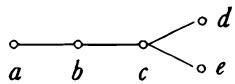
\includegraphics[keepaspectratio]{images/part001_959a1795.jpg}}

它表示一个图，其顶点为 \(a, b, c, d, e\)，其边为 \(\{a, b\}\)、\(\{b, c\}\)、\(\{c, d\}\) 和 \(\{c, e\}\)。

\appendixitem{图的连通分支}

设 \(\Gamma = (\mathbf{A},\mathbf{S})\) 是一张图。若 \(a\) 和 \(b\) 是两个顶点，则连接 \(a\) 和 \(b\) 的路是顶点序列 \((x_0,\ldots ,x_n)\)，属于图 \(\Gamma\)，满足 \(x_0 = a,x_n = b\)，且顶点 \(x_{i}\) 和 \(x_{i + 1}\) 在 \(0\leqslant i < n\) 时相连；整数 \(n\geqslant 0\) 是该路的长度。路 \((x_0,\ldots ,x_n)\) 称为单射的，当 \(x_{i}\neq x_{j}\) 对 \(i\neq j\) 成立。若路 \((x_0,\ldots ,x_n)\) 连接 \(a\) 和 \(b\)，且在这类路中长度最小，则它必为单射的；否则就存在 i 和 j，满足 \(0 \leqslant i < j \leqslant n\) 且 \(x_{i} = x_{j}\)，于是序列

\[
\left(x _ {0}, \dots , x _ {i}, x _ {j + 1}, \dots , x _ {n}\right)
\]

则会是一条连接 a 和 b 的长度为 \textless{} n 的路。

两个顶点 a 和 b 之间的关系 ``存在一条连接 a 和 b 的路'' 是 \(\Gamma\) 的一个等价关系 R，它定义在顶点集合 S 上。R 的等价类称为 \(\Gamma\) 的连通分支；如果 S 至多有一个连通分支，即 \(\Gamma\) 的任意两个顶点之间至少可以连一条路，则称 \(\Gamma\) 是连通的。

命题 1. 设 \(\Gamma = (A, S)\) 是一张图，\((S_{\alpha})_{\alpha \in L}\) 是它的连通分支族。记 \(\Gamma_{\alpha}\) 为 \(\Gamma\) 的满子图，其顶点集合为 \(S_{\alpha}\)。

\begin{enumerate}
\def\labelenumi{(\roman{enumi})}
\item
  对于 L 中任意 \(\alpha\)，图 \(\Gamma_{\alpha}\) 是连通的。
\item
  若 \(\Gamma' = (A', S')\) 是 \(\Gamma\) 的连通子图，则存在 L 中的 \(\alpha\)，使得 \(\Gamma' \subset \Gamma_{\alpha}\)。
\item
  若 \(\alpha \neq \beta\)，则 \(S_{\alpha}\) 的任何元素都不与 \(\Gamma\) 中 \(S_{\beta}\) 的任何元素相连（等价地，\(\Gamma\) 的每条边都是某个 \(\Gamma_{\alpha}\) 的边）。
\item
  设 \((\mathrm{S}_{\lambda}^{\prime})_{\lambda \in \mathbb{M}}\) 是 \(S\) 的一个划分，且若 \(\lambda \neq \mu\)，则 \(\mathrm{S}_{\lambda}^{\prime}\) 的任何元素都不与 \(\Gamma\) 中的 \(\mathrm{S}_{\mu}^{\prime}\) 的任何元素相连；则每个集合 \(\mathrm{S}_{\lambda}^{\prime}\) 都是 \(\Gamma\) 的连通分支的并集。
\item
  设 \(\alpha\) 属于 L，且 \(a\) 和 \(b\) 属于 \(S_{\alpha}\)。则存在一条路 \(c = (x_0, \ldots, x_n)\)，连接 \(a\) 和 \(b\)，位于 \(\Gamma\) 中。对于任意 \(i\)，满足 \(0 \leqslant i \leqslant n\)，路 \((x_0, \ldots, x_i)\) 连接 \(a\) 和 \(x_i\)，位于 \(\Gamma\) 中，所以 \(x_i \in S_{\alpha}\)。因此，\(c\) 是 \(\Gamma_{\alpha}\) 中连接 \(a\) 和 \(b\) 的一条路。由此 \(\Gamma_{\alpha}\) 是连通的。
\item
  设 \(\Gamma' = (A', S')\) 是 \(\Gamma\) 的一个非空连通子图，设 \(a\) 是 \(S'\) 的一个元素，且 \(S_{\alpha}\) 是 \(S\) 中包含 \(a\) 的连通分支。对于任意 \(b\)，它属于 \(S'\)，存在一条路 \(c\)，连接 \(a\) 和 \(b\)，位于 \(\Gamma'\) 中，从而 \(a\) 更不用说也位于 \(\Gamma\) 中。由此 \(S' \subset S_{\alpha}\)。
\item
  给定不同的元素 \(\alpha\) 和 \(\beta\)，它们属于 \(L\)，以及顶点 \(a \in S_{\alpha}\) 和 \(b \in S_{\beta}\)，不存在连接 \(a\) 和 \(b\) 的路，特别地，不存在连接 \(a\) 和 \(b\) 的边。
\item
  设 \(a\) 属于 \(S_{\lambda}'\)，且 \(S_{\alpha}\) 是 \(\Gamma\) 的连通分支，包含 \(a\)。于是，对于任意 \(b\)，它属于 \(S_{\alpha}\)，存在一条路 \((x_0, \ldots, x_n)\)，连接 \(a\) 和 \(b\)，位于 \(\Gamma\) 中。若 \(i\) 是满足 \(0 \leqslant i < n\) 的整数，且 \(x_i \in S_{\lambda}'\)，则 \(x_{i+1} \in S_{\lambda}'\)，因为 \(x_i\) 与 \(x_{i+1}\) 相连。由归纳法可知，\(x_i \in S_{\lambda}'\) 对 \(0 \leqslant i \leqslant n\) 成立，特别地，\(b = x_n\) 属于 \(S_{\lambda}'\)。因此，\(S_{\alpha} \subset S_{\lambda}'\)。
\end{enumerate}

推论 1. 图 \(\Gamma = (A, S)\) 连通，当且仅当不存在一个划分 \((S', S'')\)，将 \(S\) 分成两个非空子集，并且 \(S'\) 的任何元素都不与 \(\Gamma\) 中的 \(S''\) 的任何元素相连。

假设 \(\Gamma\) 不连通，并令 \(S'\) 为其一个连通分支。集合 \(S'' = S - S'\) 根据命题 1 (i) 是非空的，并且根据命题 1 (iii)，\(S'\) 的任何元素都不与 \(S''\) 的任何元素相连。

现在假设 \(\Gamma\) 连通，并设 \((S', S'')\) 是具有所述性质的一个划分。根据命题 1 (iv)，集合 \(S'\) 包含至少一个连通分支，因此 \(S' = S\) 且 \(S'' = \varnothing\)，矛盾。

推论 2. 一个子集 \(S'\)（\(S\) 的子集）是连通分支的并集，当且仅当属于 \(S'\) 的任何顶点都不与属于 \(S - S'\) 的任何顶点相连。

该条件由命题 1 (iv) 充分。由命题 1 (iii)，该条件也是必要的。


\appendixitem{森林与树}

设 \(\Gamma = (\mathrm{A},\mathrm{S})\) 为一个图。\(\Gamma\) 的一个回路是一个序列

\[
(x _ {1}, \ldots , x _ {n})
\]

其中 \(\Gamma\) 的各顶点互不相同，并且满足 \(n \geqslant 3\)、\(x_{i}\) 与 \(x_{i+1}\) 相连（\(1 \leqslant i < n\)），且 \(x_{n}\) 与 \(x_{1}\) 相连。若 \(\Gamma\) 中没有回路，则称 \(\Gamma\) 为森林；于是 \(\Gamma\) 的每个子图也都是森林。连通的森林称为树；因此森林的连通分支都是树。

命题 2. 设 \(\Gamma = (\mathrm{A},\mathrm{S})\) 是只有有限个顶点的森林。

\begin{enumerate}
\def\labelenumi{(\roman{enumi})}
\item
  若 \(\Gamma\) 至少有一个顶点，则它有一个端点。
\item
  若 \(\Gamma\) 至少有两个顶点，则其顶点集可以划分为两个非空子集 \((\mathbf{S}', \mathbf{S}'')\)，使得同属 \(\mathbf{S}'\) 或同属 \(\mathbf{S}''\) 的两个不同顶点从不相连。
\end{enumerate}

设 \(\Gamma\) 至少有一个顶点，并令 \((x_{0},\ldots,x_{n})\) 为 \(\Gamma\) 中长度最大的单射路径。顶点 \(x_{0}\) 不可能与一个异于 \(x_{0},x_{1},\ldots,x_{n}\) 的顶点 y 相连，因为否则 \(\Gamma\) 中将存在长度为 \(n+1\) 的单射路径，即 \((y,x_{0},\ldots,x_{n})\)。顶点 \(x_{0}\) 不与任何顶点 \(x_{i}\)（满足 \(2\leqslant i\leqslant n\)）相连，因为否则 \((x_{0},x_{1},\ldots,x_{i})\) 将是森林 \(\Gamma\) 中的回路。因此，\(x_{0}\) 是端点。

我们按顶点数 \(m\) 的 \(\Gamma\) 对 (ii) 作归纳证明，\(m = 2\) 的情形是显然的。于是设 \(m \geqslant 3\)，并且断言 (ii) 对有 \(m - 1\) 个顶点的图已经得到证明。令 \(a\) 为 \(\Gamma\) 的一个端点（参见 (i)）。我们将归纳假设应用于 \(\Gamma\) 的全子图，该子图的顶点是满足 \(x \neq a\) 的、属于 \(\Gamma\) 的顶点。因此，存在两个不相交的非空子集 \(S_1'\) 和 \(S_1''\)（它们属于 \(S\)），满足 \(S_1' \cup S_1'' = S - \{a\}\)，并且 \(S_1'\) 中（分别，\(S_1''\) 中）的两个不同顶点从不相连。由于 \(a\) 至多与 \(\Gamma\) 的一个顶点相连，我们不妨设它不与 \(S_1'\) 中任何顶点相连。于是划分 \((S_1', S_1'' \cup \{a\})\) 具有所需性质。证毕。

对于任意整数 \(n \geqslant 1\)，以 \(A_{n}\) 表示如下图：其顶点是整数 \(1, 2, \ldots, n\)，其边是形如 \(\{i, j\}\) 的对，其中 \(i - j = \pm 1\)：

1

2

3

n---1

n

○

○

○

\ldots\ldots{}

○

若图 \(\Gamma\) 被称为长度为 \(m \geqslant 0\) 的链，当且仅当它同构于 \(A_{m+1}\)。这等价于：\(\Gamma\) 中存在包含所有顶点的单射路径 \((x_{0}, \ldots, x_{m})\)，且顶点 \(x_{i}\) 与 \(x_{j}\) 不相连（若 \(|i-j| > 1\)）。

命题 3. 一个图是链，当且仅当它的顶点数有限且非零，并且它是一棵没有分叉点的树。

设图 \(\Gamma\) 是具有命题 3 之前所列性质的链 \((x_0, \ldots, x_m)\)。显然，\(\Gamma\) 的任一顶点至多与两个顶点相连。若 \(i < j\)，则路径 \((x_i, \ldots, x_j)\) 是从路径 \((x_0, \ldots, x_m)\) 中取出的，并将 \(x_i\) 与 \(x_j\) 相连；因此，\(\Gamma\) 是连通的。最后，设 \((x_{p_1}, \ldots, x_{p_n})\) 是 \(\Gamma\) 中的一个回路，并令 \(p_k\) 为互不相同的整数 \(p_1, \ldots, p_n\) 中最小者。存在不同的指标 \(i\) 和 \(j\)，使得 \(x_{p_k}\) 分别与 \(x_{p_i}\) 和 \(x_{p_j}\) 相连：这由回路的定义可知。由于 \(p_k < p_i\) 且 \(p_k < p_j\)，必有 \(p_i = p_j = p_k + 1\)，这与 \(p_1, \ldots, p_n\) 互不相同矛盾。因此，\(\Gamma\) 中没有回路。

反之，设 \(\Gamma\) 是一棵没有分叉点且顶点数有限非零的树，并令 \((x_0, \ldots, x_m)\) 为 \(\Gamma\) 中长度最大的单射路径。以 T 表示除 \(x_0, \ldots, x_m\) 外的顶点集。顶点 \(b \in T\) 不可能与任何顶点 \(x_i\) 相连，因为那样我们将有以下情形之一：

\begin{enumerate}
\def\labelenumi{\alph{enumi})}
\item
  \(i = 0\)，但此时 \((b, x_0, \ldots, x_m)\) 将是长度为 \(m + 1\) 且位于 \(\Gamma\) 中的单射路径；或
\item
  \(i = m\)，但此时 \((x_0, \ldots, x_m, b)\) 将是长度为 \(m + 1\) 且位于 \(\Gamma\) 中的单射路径；或
\item
  \(0 < i < m\)，但此时 \(x_{i}\) 将与三个不同的顶点 \(x_{i-1}\)、\(x_{i+1}\) 和 \(b\) 相连。
\end{enumerate}

由于 \(\Gamma\) 是连通的，由命题 1 的推论 1，\(T\) 为空。此外，若存在 \(i,j\) 满足 \(j - i > 1\) 且 \(x_{i}, x_{j}\) 相连，则将有回路 \((x_{i}, x_{i+1}, \ldots, x_{j})\) 位于 \(\Gamma\) 中。因此，\(\Gamma\) 是链。证毕。

\exercisesection{§ 1 的习题}

\begin{enumerate}
\def\labelenumi{\arabic{enumi})}
\tightlist
\item
  \begin{enumerate}
  \def\labelenumii{\alph{enumii})}
  \tightlist
  \item
    设 (W, S) 为 Coxeter 系统，并设 \(s_{1}, \ldots, s_{r}\) 是 S 的元素。置 \(w = s_{1} \ldots s_{r}\)。证明：若 \(l_{\mathbb{S}}(w) < r\)，则存在两个整数 p、q，满足 \(1 \leqslant p < q \leqslant r\)，使得 \(w = s_{1} \ldots s_{p-1}s_{p+1} \ldots s_{q-1}s_{q+1} \ldots s_{r}\)。证明存在严格递增的整数序列 \(j(1), \ldots, j(k)\)，其各项介于 1 与 r 之间，使得 \((s_{j(1)}, \ldots, s_{j(k)})\) 是 w 的一个约化分解。
  \end{enumerate}
\end{enumerate}

\begin{enumerate}
\def\labelenumi{\alph{enumi})}
\setcounter{enumi}{1}
\tightlist
\item
  设 \((\mathbf{W},\mathbf{S})\) 为 Coxeter 系统，且 \(X,Y,Z\) 为 \(S\) 的三个子集。证明
\end{enumerate}

\[
W _ {X} \cap (W _ {Y}. W _ {Z}) = (W _ {X} \cap W _ {Y}). (W _ {X} \cap W _ {Z})
\]

（证明每个元素 \(w \in W_{Y}.W_{Z}\) 都有一个约化分解

\[
(s _ {1}, \ldots , s _ {h}, t _ {1}, \ldots , t _ {k})
\]

其中 \(s_i \in Y\)、\(t_j \in Z\)，并使用第 8 项命题 7 的推论 1）。

证明

\[
W _ {X}. \left(W _ {Y} \cap W _ {Z}\right) = \left(W _ {X}. W _ {Y}\right) \cap \left(W _ {X}. W _ {Z}\right).
\]

\begin{enumerate}
\def\labelenumi{\arabic{enumi})}
\setcounter{enumi}{1}
\item
  设 \((W,S)\) 为 Coxeter 系统，X 为 S 的一个子集。证明：\(W_{X}\) 在 W 中正规，当且仅当 X 的每个元素都与 S-X 的每个元素交换。
\item
  设 \((\mathbf{W},\mathbf{S})\) 为 Coxeter 系统，\(\mathbf{X},\mathbf{Y}\) 为 \(\mathbf{S}\) 的两个子集。令 \(a\in W\)。证明存在唯一的最短元素 \(w\in W_X a W_Y\)，并且每个元素
\end{enumerate}

\[
w ^ {\prime} \in W _ {X} a W _ {Y}
\]

可以写成 \(w' = xwy\) 的形式，其中 \(x \in W_X, y \in W_Y\)，且 \(l(w') = l(x) + l(w) + l(y)\)（取 \(W_X aW_Y\) 中的最短元素并使用习题 1）。称元素 \(w \in W\) 为 \((X,Y)\)-约化的，如果它是双陪集 \(W_X aW_Y\) 中的最短元素。

证明：若 \(w\) 是 \((X, \emptyset)\)-约化的，则有 \(l(xw) = l(x) + l(w)\) 对所有 \(x \in W_X\) 成立，并且 \(W\) 的每个元素都能唯一地写成 \(xw\) 的形式，其中 \(x \in W_{X}\)，而 w 是 \((X, \varnothing)\)-约化的。证明元素 \(w \in W\) 是 \((X, \varnothing)\)-约化的，当且仅当 \(l(xw) > l(w)\) 对所有 \(x \in X\) 成立（将 w 写成 \(yw'\) 的形式，其中 \(y \in W_{X}\)，而 \(w'\) 是 \((X, \varnothing)\)-约化的）。

证明 \(w \in W\) 是 \((X, Y)\)-约化的，当且仅当 w 同时是 \((X, \varnothing)\)-约化的和 \((\varnothing, Y)\)-约化的。

\begin{enumerate}
\def\labelenumi{\arabic{enumi})}
\setcounter{enumi}{3}
\item
  设 \(n\) 为一个整数 \(\geqslant 2\)。对于任意整数 \(i\) 满足 \(1 \leqslant i \leqslant n - 1\)，以 \(s_i\) 表示 \(i\) 与 \(i + 1\) 在集合 \(\{1, 2, \ldots, n\}\) 中的换位，以 \(H_i\) 表示 \(w \in \mathfrak{S}_n\) 且满足 \(w^{-1}(i) < w^{-1}(i + 1)\) 的 w 的集合；置 \(S = \{s_1, \ldots, s_{n-1}\}\)。证明 \((\mathfrak{S}_n, S)\) 是 Coxeter 系统，并且 \(H_i\) 是 \(w \in \mathfrak{S}_n\) 中满足 \(l(w) < l(s_i w)\) 的那些 w 的集合（使用第 7 项命题 6）。
\item
  设 X 是一个非空集合，W 是 X 上的一组置换。给定 X 上等价关系的集合 R、元素 \(x_{0} \in X\) 以及从 R 到 W 的映射 \(\varphi : H \mapsto s_{H}\)。以 \(R_{0}\) 表示满足如下条件的 \(H \in R\) 的集合：\(s_{\mathrm{H}}(x_{0}) \equiv x_{0} \mod \mathrm{H}'\) 对 R 中所有 \(H' \neq H\) 均成立；以 \(S_{0}\) 表示这些 \(s_{H}\)（其中 H 属于 \(R_{0}\)）所成的集合。作如下假设：
\end{enumerate}

\begin{enumerate}
\def\labelenumi{(\roman{enumi})}
\item
  对任意 \(\mathbf{H} \in \Re\)，模 \(\mathbf{H}\) 有两个等价类被 \(s_{\mathrm{H}}\) 置换，且 \(s_{\mathrm{H}}^{2} = 1\)。
\item
  对所有 \(\mathbf{H} \in \Re\) 和所有 \(w \in \mathbf{W}\)，\(w(\mathbf{H})\) 是 \(\mathbf{H}\) 在 \(w\) 下的变换，属于 \(\Re\) 的等价关系，且 \(s_{w(\mathbf{H})} = ws_{\mathbf{H}}w^{-1}\)。
\item
  对任意 \(w \neq 1\)（在 \(W\) 中），\(H \in \Re\) 中使 \(w(x_0) \not\equiv x_0 \mod H\) 的那些 H 所成的集合是有限的，并且与 \(\Re_0\) 相交。
\end{enumerate}

\begin{enumerate}
\def\labelenumi{\alph{enumi})}
\item
  证明 \((\mathbf{W},\mathbf{S}_0)\) 是 Coxeter 系统（使用第 7 项命题 6）。
\item
  证明长度 \(l_{S_0}(w)\) 等于满足下式的 \(H \in \mathfrak{R}\) 的元素个数：
\end{enumerate}

\[
w (x _ {0}) \not \equiv x _ {0} \bmod . H.
\]

\begin{enumerate}
\def\labelenumi{\alph{enumi})}
\setcounter{enumi}{2}
\tightlist
\item
  设 E 是一个有限集，X 是 X 上全序关系的集合。以 W 表示 E 的置换群，它以显然的方式作用于 E。设 i、j 是 E 的不同元素；如果 X 的两个元素 R、R' 模 \(H_{ij}\) 等价，即满足 \(\mathrm{R}(i,j)\) 与 \(\mathrm{R}'(i,j)\)，或者满足 \(\mathrm{R}(j,i)\) 与 \(\mathrm{R}'(j,i)\)，则称它们等价；以 \(s_{ij}\) 表示 i 与 j 的换位。令 R 为形如 \(H_{ij}\) 的等价关系的集合，并令 \(\varphi\) 为从 R 到 W 的映射，由 \(\varphi(\mathrm{H}_{ij}) = s_{ij}\) 定义；最后令 \(x_{0}\) 为 X 的任意元素。证明如此定义的对象满足假设 (i) 至 (iii)，并重新得到习题 4 的结果。
\end{enumerate}

\begin{enumerate}
\def\labelenumi{\arabic{enumi})}
\setcounter{enumi}{5}
\item
  设 E 是含有 6 个元素的集合，F 是 E 上域 \(F_{5}\) 的射影直线结构的集合。以 \(S_{E}\) 表示 E 的置换群；对任意 \(\sigma \in S_{E}\)，以 \(\tilde{\sigma}\) 表示 \(\sigma\) 通过结构传递在 F 上诱导的置换。证明存在从 E 到 F 的双射 u，并且映射 \(\sigma \mapsto u^{-1}\tilde{\sigma}u\) 是 \(S_{E}\) 的外自同构（若 s 是换位，则 \(u^{-1}\tilde{s}u\) 有三个二元轨道）。
\item
  构造一个群 W 及其两个子集 S、S'，使得 (W, S) 与 (W, S') 是同构的 Coxeter 系统，但不存在将 S 变为 S' 的 W 的内自同构（使用习题 4 和习题 6）。
\item
  构造一个群 W 及其两个子集 S、S'，使得 (W, S) 与 (W, S') 是不同构的 Coxeter 系统，其中一个不可约而另一个可约（令 W 为由 \(\{s, s'\}\) 生成的 12 阶二面体群，其中 s 和 \(s'\) 的阶为 2 且 \(s \neq s'\)，并置 \(S = \{s, s'\}\)、\(S' = \{(ss')^3, s', s'(ss')^2\}\)）。
\item
  设 (W, S) 是矩阵 \((m(s, s'))\) 给出的 Coxeter 系统，并令 \(W^{+}\) 为由 W 中长度为偶数的元素组成的子群。令 \(s_{0} \in S\)。置 \(g_{s} = ss_{0}\)。证明族 \((g_{s})_{s \in S - \{s_{0}\}}\)，以及关系 \(g_{s}^{m(s, s_{0})} = 1\)（当 \(m(s, s_{0}) \neq \infty\)）和关系 \((g_{s} g_{s'}^{-1})^{m(s, s')} = 1\)（当 \(s, s' \in S - \{s_{0}\}\) 且 \(m(s, s') \neq \infty\)），构成 \(W^{+}\) 的一个表示。（令 \(H^{+}\) 为上述表示定义的群。证明存在一个平方为恒等的自同构 \(\alpha\)，其定义在 \(H^{+}\) 上，将 \(g_{s}\) 变为 \(g_{s}^{-1}\)（对所有 \(s \in S - \{s_{0}\}\)）。若 \(H_{\alpha}\) 是 \(\{1, -1\}\) 与 \(H^{+}\) 关于 \(\alpha\) 的半直积，定义互为逆的同态 \(H_{\alpha} \to W\) 和 \(W \to H_{\alpha}\)。）证明：若 S 的元素彼此共轭（参见命题 3），则群 \(W^{+}\) 是 W 的换位子群（注意此时元素 \(g_{s}\) 都是换位子）。
\item
  令 \(\mathfrak{U}_n\) 为由置换 \(w \in \mathfrak{S}_n\) 中符号等于 \(+1\) 的那些置换组成的交错群。证明 \(\mathfrak{U}_n\) 是 \(\mathfrak{S}_n\) 的换位子群（使用习题 4 和 9）。对于任意整数 \(i\) 满足 \(1 \leqslant i \leqslant n - 2\)，置 \(u_i = s_i s_{i+1}\)（沿用习题 4 的记号）。证明族 \((u_i)\)，以及关系 \(u_1^3 = 1\)、\(u_i^2 = 1\)（当 \(i \geqslant 2\) 时）、\((u_i u_{i+1})^3 = 1\)（当 \(1 \leqslant i \leqslant n - 3\) 时）和 \(u_i u_j = u_j u_i\)（当 \(1 \leqslant i \leqslant n - 4\) 且 \(i + 2 \leqslant j \leqslant n - 2\) 时）构成群 \(\mathfrak{U}_n\) 的一个表示（使用习题 9）。
\end{enumerate}

*11) 令 \((\mathbf{W},\mathbf{S})\) 为 Coxeter 系统。令 \(\Gamma_{\infty}\) 为顶点集是 \(\mathbf{S}\) 的图；两个顶点 \(s,s'\) 以一条边相连，当且仅当 \(m(s,s')\neq \infty\)。令 \(\mathrm{S}_{\alpha}\) 为 \(\Gamma_{\infty}\) 的连通分支。证明 \(\mathbf{W}\) 可以认作各 \(\mathrm{W}_{\mathrm{S}_{\alpha}}\) 的自由积。特别地，每个元素 \(w\in \mathbf{W}\) 都能唯一地写成乘积 \(w_{1}\ldots w_{h}\)，其中 \(w_{i}\neq 1\)，\(w_{i}\) 属于 \(\mathrm{W}_{\mathrm{S}_{\alpha_i}}\)，且有 \(\alpha_{i}\neq \alpha_{i + 1}\)（\(1\leqslant i\leqslant h - 1\)）；证明 \(w\) 的长度等于各 \(w_i\) 的长度之和。*

\begin{enumerate}
\def\labelenumi{\arabic{enumi})}
\setcounter{enumi}{11}
\tightlist
\item
  设 \((\mathbf{W},\mathbf{S})\) 为 Coxeter 系统，满足 \(m(s,s')\) 在 \(s\neq s'\) 时为偶数，并令 \(\mathbf{X}\) 为 \(\mathbf{S}\) 的一个子集。证明存在唯一的同态 \(f_{\mathbf{X}}\)，从 \(\mathbf{W}\) 到 \(\mathbf{W}_{\mathbf{X}}\)，满足 \(f_{\mathbf{X}}(s) = s\)（当 \(s\in \mathbf{X}\)）且 \(f_{\mathbf{X}}(s) = 1\)（当 \(s\in \mathbf{S} - \mathbf{X}\)）。推出 \(\mathbf{W}\) 是 \(\mathbf{W}_{\mathbf{X}}\) 与 \(f_{\mathbf{X}}\) 的核的半直积。证明：若 \(\mathbf{X}\subset \mathbf{Y}\subset \mathbf{S}\)，则存在唯一的同态 \(f_{\mathbf{X},\mathbf{Y}}\)，从 \(\mathbf{W}_{\mathbf{Y}}\) 到 \(\mathbf{W}_{\mathbf{X}}\)，满足 \(f_{\mathbf{X}} = F_{\mathbf{X},\mathbf{Y}}\circ f_{\mathbf{Y}}\)，并且 \(\mathbf{W}\) 可以认作由 X 遍历 S 的有限子集所得到的滤过集上的 \(W_{X}\) 的射影系统的一个子群。
\end{enumerate}

¶ 13) 设 \((W, S)\) 为 Coxeter 系统。对 \(s, s' \in S\)，按以下规则定义序列 \(\mathbf{a}(s, s')\)：

\begin{enumerate}
\def\labelenumi{(\roman{enumi})}
\item
  若 \(ss'\) 的阶为无穷，则 \(\mathbf{a}(s, s')\) 是空序列；
\item
  若 \(ss'\) 的阶为有限数 m，则序列 \(\mathbf{a}(s, s')\) 的长度为 m，且其偶数编号项（分别为奇数编号项）等于 \(s'\)（分别为 s）。
\end{enumerate}

以 \(a(s, s')\) 表示序列 \(\mathbf{a}(s, s')\) 的乘积。

\begin{enumerate}
\def\labelenumi{\alph{enumi})}
\item
  证明生成集 S 以及关系 \(s^{2}=1\) 和 \(\mathbf{a}(s,s')=\mathbf{a}(s',s)\) 构成群 W 的一个表示。
\item
  令 \(q\) 为一个整数 \(\geqslant 1\)。令 \(\Sigma_q\) 为由 \(q\) 个 \(S\) 的元素组成的序列的集合，并令 \(R_q\) 为 \(\Sigma_q\) 上的最小等价关系，使得形如 \((A, \mathbf{a}(s, s'), B)\) 和 \((A, \mathbf{a}(s', s), B)\) 的序列（其中 \(s, s' \in S\)，且 \(A\) 和 \(B\) 是由 \(S\) 的元素组成的序列）等价。令 \(\Sigma_q^r\) 为序列 \(\mathbf{s} = (s_1, \ldots, s_q)\) 的集合，其中 \(w(\mathbf{s}) = s_1 \ldots s_q\) 的长度为 \(q\)。证明序列 \(\mathbf{s}, \mathbf{s}' \in \Sigma_q^r\) 模 \(R_q\) 等价，当且仅当 \(w(\mathbf{s}) = w(\mathbf{s}')\)（按 \(q\) 归纳，并应用第 5 项命题 5）。
\item
  证明序列 \(\mathbf{s} \in \Sigma_q\) 不属于 \(\Sigma_q^r\)，当且仅当 \(\mathbf{s}\) 模 \(R_q\) 等价于一个含有两个相邻相等项的序列。（按 \(q\) 归纳，并归结为序列 \((s_1, \ldots, s_q)\) 的情形：它不属于 \(\Sigma_q^r\)，但 \((s_1, \ldots, s_{q-1})\) 和 \((s_2, \ldots, s_q)\) 属于 \(\Sigma_{q-1}^r\)；使用习题 1 证明 \(s_1 \ldots s_{q-1} = s_2 \ldots s_q\)，再应用 b)。
\end{enumerate}

*14) 设 \((\mathbf{W},\mathbf{S})\) 为 Coxeter 系统，\((\Gamma ,f)\) 为其 Coxeter 图。令 \(k\) 为一个整数 \(\geqslant 3\)。若 \(a\) 是 \(\Gamma\) 的一条边，则置 \(f_{k}(a) = f(a)\)（当 \(f(a)\neq \infty\) 时），并置 \(f_{k}(a) = k\)（当 \(f(a) = \infty\) 时）。令 \((\mathrm{W}_k,\mathrm{S})\) 为 Coxeter 图等于 \((\Gamma ,f_k)\) 的 Coxeter 系统（第 V 章，§4，第 3 项命题 4 的推论）。证明存在唯一的同态 \(\varphi_{k}\)，从 W 到 \(\mathbf{W}_k\)，在 S 上诱导恒等映射。证明若 \(k\) 整除 \(k^{\prime}\)，则存在唯一的同态 \(\varphi_{k,k^{\prime}}\)，从 \(\mathbf{W}_{k^{\prime}}\) 到 \(\mathbf{W}_k\)，满足 \(\varphi_{k} = \varphi_{k,k^{\prime}}\circ \varphi_{k^{\prime}}\)。证明同态 \((\varphi_{k})\) 从 W 到 \(\mathbf{W}_k\) 的射影极限是单射（使用习题 13）\(c)\)，但一般不是满射（例如在无限二面体群的情形）。*

\begin{enumerate}
\def\labelenumi{\arabic{enumi})}
\setcounter{enumi}{14}
\tightlist
\item
  设 A 是一个集合，C 是 \(\mathfrak{P}(A)\) 的一个子集。C 的元素称为 A 的室，室 C 的子集 F 称为一个面，并将 F 在 C 中的余维定义为 C-F 的基数。若面 F 在 C 中的余维为 1，则称 F 为 C 的一个面板。若两个室 C、C' 有公共面板 F，则称它们相邻：此时或者 \(C = C'\)，或者 \(F = C \cap C'\)。长度为 n 的廊是序列 \(\Gamma = (C_0, C_1, \ldots, C_n)\)，由 \(n + 1\) 个室组成，并满足 \(C_i\) 与 \(C_{i+1}\) 相邻（\(0 \leqslant i \leqslant n - 1\)）。于是称 \(C_0\) 与 \(C_n\) 为 \(\Gamma\) 的端点。廊 \(\Gamma\) 称为单射的，当 \(C_i \neq C_{i+1}\)（\(0 \leqslant i \leqslant n - 1\)）时；若不存在具有相同端点且长度 \textless{} n 的廊，则称其为最短的。
\end{enumerate}

若 A 的每个元素至少属于一个室，且任意两个室都是某个廊的端点，则称 A（连同 C）为一个建筑。两个室 C 与 \(C'\) 之间的距离，是长度 \(d(\mathrm{C},\mathrm{C}')\) 的、端点为 C 与 \(C'\) 的最短廊。

A 的一个子建筑是 A 的子集 D，使得 D 连同 \(\mathfrak{C}\cap\mathfrak{P}(D)\) 构成一个建筑。

\begin{enumerate}
\def\labelenumi{\alph{enumi})}
\item
  证明：若 A 是一个建筑，则一个面在包含它的每个室中的余维相同；因此，我们可以不指明特定的室而谈论 A 的面的余维和面板。建筑 B 到 A 的态射是从 B 到 A 的映射 f，使得 f 在 B 的每个室 C 上的限制是从 C 到 A 的一个室 \(f(\mathrm{C})\) 的双射。证明 B 的一个面在 f 下的像仍是具有相同余维的面。
\item
  若每个面板恰好包含于两个室中，则称建筑 A 为一个公寓。证明：若 A 是一个公寓，则 A 的每个保持 C 不变的自同构（即 A 的每个保持 C 的置换）若固定一个室的所有点，就必为恒等映射。更一般地，设 \(\varphi\) 是 A 的一个自同态，C 是 A 的一个室，且 \(\varphi(a)=a\) 对所有 \(a\in C\) 成立。令 \((\mathrm{C},\mathrm{C}_{1},\ldots,\mathrm{C}_{n})\) 为 A 的一个廊。证明：廊 \((\mathrm{C},\varphi(\mathrm{C}_{1}),\ldots,\varphi(\mathrm{C}_{n}))\) 要么不是单射的，要么 \(\varphi(a)=a\) 对所有属于各 \(C_{i}\) 的并集的 a 都成立。
\end{enumerate}

\begin{enumerate}
\def\labelenumi{\arabic{enumi})}
\setcounter{enumi}{15}
\tightlist
\item
  设 \((W,S)\) 为 Coxeter 系统。对 \(s \in S\)，以 \(W^{(s)}\) 表示 W 的子群 \(W_{S-\{s\}}\)，以 A 表示形如 \(wW^{(s)}\)（其中 \(w \in W\) 且 \(s \in S\)）的 W 的子集所成的集合，并以 C 表示形如 \(C_w = \{wW^{(s)} \mid s \in S\}\)（其中 \(w \in W\)）的 A 的子集所成的集合；我们称这些子集为 A 的室（习题 15）。
\end{enumerate}

\begin{enumerate}
\def\labelenumi{\alph{enumi})}
\item
  证明映射 \(w \mapsto \mathbf{C}_w\) 是从 W 到 \(\mathfrak{C}\) 的双射。
\item
  证明两个不同的室 \(C_{w}\) 与 \(C_{w'}\) 相邻，当且仅当存在 \(s \in S\) 使得 \(w' = ws\)。推出 A（连同 C）是一个公寓（习题 15），我们称其为 (W, S) 的公寓。证明端点为 \(C_{w}\) 与 \(C_{w'}\) 的最短廊的长度等于 \(l_{S}(w^{-1}w')\)。
\item
  令 \(\mathfrak{F}\) 为 A 的面的集合，并令 \(F \in \mathfrak{F}\)。证明存在 S 的唯一子集 X 和 W 的一个元素 \(w \in W\)，使得 \(wW_X = \bigcap_{i \in F} i\)。于是称 F 为 X 型。证明 F 的余维等于 X 的基数。证明映射 \(j: F \mapsto \bigcap_{i \in F} i\) 是从 \(\mathfrak{F}\) 到形如 \(wW_X\)（其中 \(w \in W\)、\(X \subset S\)）的 W 的子集的严格递减双射（关于包含关系）。证明：对满足 \(X \subset Y \subset S\) 的每个 Y，每个 X 型面都包含唯一的 Y 型面。
\item
  令 W 通过左平移作用于 A，并置 \(C = C_{e}\)。证明 W 在 C 上单纯传递地作用 \(^{8}\)。令 \(C_{1}, \ldots, C_{n}\) 为 A 的室。证明以下条件等价：
\end{enumerate}

\begin{enumerate}
\def\labelenumi{(\roman{enumi})}
\item
  序列 \(\Gamma = (\mathrm{C}_0 = \mathrm{C},\mathrm{C}_1,\dots ,\mathrm{C}_n)\) 是一个单射廊；
\item
  存在由 S 的元素组成的序列 \(\mathbf{s} = (s_1, \ldots, s_n)\)，使得 \(\mathrm{C}_j = t_j(\mathrm{C}_{j-1})\) 对 \(1 \leqslant j \leqslant n\) 成立，其中 \(t_j\) 是第 4 项公式 (11) 中定义的 \(\Phi(\mathbf{s})\) 的元素。
\end{enumerate}

证明：若这些条件满足，则序列 s 是唯一的，且 \(C_{n} = s_{1} \ldots s_{n}(C)\)。证明廊 \(\Gamma\) 是最短的，当且仅当序列 \(\mathbf{s}(\Gamma) = \mathbf{s}\) 是 \(w = s_{1} \ldots s_{n}\) 的一个约化分解。

\begin{enumerate}
\def\labelenumi{\alph{enumi})}
\setcounter{enumi}{4}
\tightlist
\item
  令 T 为 S 的共轭元的并集。对 \(t \in T\)，A 中在 t 下不变的点集 \(L_{t}\) 称为 t 所定义的墙。证明 \(L_{t}\) 是面板的并集，并且面板 F 包含于 \(L_{t}\) 当且仅当 \(j(\mathrm{F})\) 形如 \(wW_{\{s\}}\)，其中 \(t = wsw^{-1}\)。推出：对任意面板 F，存在唯一的元素 \(t = t(\mathrm{F}) \in \mathrm{T}\) 使得 \(F \subset L_{t}: L_{t}\) 称为 F 的支撑墙。
\end{enumerate}

证明：若 \(w(\mathrm{L}_t) = \mathrm{L}_t\)（其中 \(w \in \mathrm{W}\)），则 \(w = 1\) 或 \(w = t\)。

\(f)\) 令 \(w', w'' \in W\)。置 \(C' = w'(C), C'' = w''(C)\)，并令 \(\Gamma = (C_0 = C', C_1, \ldots, C_n = C'')\) 为端点为 \(C'\) 和 \(C''\) 的单射廊。令 \(t_j\) 为 \(T\) 中定义面板 \(C_j \cap C_{j-1}\) 的支撑墙的元素（当 \(1 \leqslant j \leqslant n\) 时）。证明序列 \(\Psi(T) = (w'^{-1} t_j w')_{1 \leqslant j \leqslant n}\) 与序列 \(\Phi(s(w'^{-1}(\Gamma))\) 重合。对 \(t \in T\)，令 \(n(\Gamma, t)\) 为 \(w'^{-1} tw'\) 在 \(\Psi(\Gamma)\) 中出现的次数。由第 4 项引理 1 推出，数 \((-1)^{n(\Gamma, t)}\) 只依赖于 \(C'\) 和 \(C''\)，而不依赖于 \(\Gamma\)：记其为 \(\eta(C', C'', t)\)。证明关系 \(\eta(C', C'', t) = 1\) 是 \(C'\) 与 \(C''\) 之间的一个等价关系，并且有两个被 \(t\) 置换的等价类。以 \(\mathfrak{C}^+(t)\) 表示包含 \(C\) 的等价类，以 \(\mathfrak{C}^-(t)\) 表示另一个等价类。

证明：对 \(w \in \mathbf{W}\) 和 \(s \in S\)，室 \(w(\mathbf{C})\) 属于 \(\mathfrak{C}^+(s)\)，当且仅当 \(l(sw) > l(w)\)。

\(g)\) 令 \(\mathrm{A}^{+}(t)\)（分别为 \(\mathrm{A}^{-}(t)\)）为属于 \(\mathfrak{C}^{+}(t)\)（分别为 \(\mathfrak{C}^{-}(t)\)）的室的并集（其中 \(t \in \mathrm{T}\)）。证明 \(\mathrm{A}^{+}(t) \cap \mathrm{A}^{-}(t) = \mathrm{L}_{t}\)。（为证明 \(\mathrm{A}^{+}(t) \cap \mathrm{A}^{-}(t) \subset \mathrm{L}_{t}\)，归结到 \(t \in \mathrm{S}\) 的情形。若 \(a \in \mathrm{A}^{+}(t) \cap \mathrm{A}^{-}(t)\)，置 \(a = w\mathrm{W}^{(s)}\)，其中 \(s \in \mathrm{S}\)，且 \(w\) 是 \((\varnothing, \mathrm{S} - \{s\})\)-约化的（习题 3）。若 \(w(\mathrm{C}) \in \mathfrak{C}^{-}(t)\)，则 \(l(tw) < l(w)\)，且 \(w = ts_{1}, \ldots, s_{q}\)，其中 \(s_{j} \in \mathrm{S}\) 且 \(l(w) = q + 1\)。由于 \(a \in \mathrm{A}^{-}(t)\)，存在 \(x \in \mathrm{W}^{(s)}\)，使得 \(wx(\mathrm{C}) \in \mathfrak{C}^{+}(t)\)。于是

\[
l (t w x) = 1 + l (w x) = 1 + l (w) + l (x),
\]

但由于 \(twx = s_1 \ldots s_q x\)，这是矛盾。因此，\(w(\mathbf{C}) \in \mathfrak{C}^+(t)\) 且 \(l(tw) = 1 + l(w)\)。若 \(x \in \mathrm{W}^{(s)}\) 满足 \(l(twx) < l(wx)\)，则由习题 1 推出 \(twx = wx'\)，其中 \(x' \in \mathrm{W}^{(s)}\)，从而 \(ta = a\) 且 \(a \in \mathrm{L}_t\)。

子集 \(\mathbf{A}^{+}(t)\) 和 \(\mathbf{A}^{-}(t)\) 称为由墙 \(L_{t}\) 确定的 A 的两个半部。若 A 的两个点属于（分别不同时属于）两个半部之一，则称它们位于 \(L_{t}\) 的同侧（分别严格位于两侧）。任一面都包含于由 \(L_{t}\) 确定的某个半部中。若两个面包含于不同的半部中，则称它们位于 \(L_{t}\) 的两侧，或称被 \(L_{t}\) 分隔。

\(h\)）令 \(w \in \mathbf{W}\)。证明 \(l(w)\) 等于分隔 \(\mathbf{C}\) 与 \(w(\mathbf{C})\) 的墙的数目。

\begin{enumerate}
\def\labelenumi{\roman{enumi})}
\tightlist
\item
  证明映射 \(\varphi\) 将半部 \(A^{+}(t)\)（分别将 \(A^{-}(t)\)）映到 \((1,t)\)（分别映到 \((-1,t)\)），是从半部集合 \(\mathfrak{M}\) 的 \(A\) 到集合 \(R = \{1, - 1\} \times T\) 的双射（参见第 4 项）。沿用第 4 项引理 1 的记号，证明 \(\varphi(w(M)) = U_w(\varphi(M))\) 对所有 \(w\in W\) 和 \(M\in \mathfrak{M}\) 成立。
\end{enumerate}

\begin{enumerate}
\def\labelenumi{\arabic{enumi})}
\setcounter{enumi}{16}
\item
  沿用习题 16 的记号，并假设 W 有限。令 H 为 A 的墙的集合。对任意 \(H \in H\)，将 A 中由 H 确定且包含 C 的半部 \(H^{+}\) 与之关联。证明可以对 H 的元素编号，使映射 \(j \mapsto \bigcap_{i \leqslant j} H_{i}^{+}\) 在区间 {[}1, \(\operatorname{Card}(\mathfrak{H})\) {]} 上严格递减。（考虑族 \(\mathfrak{F}\)，它由集合 \(\mathrm{H}^{+}\) 的交按包含关系排序而成，并考虑 \((\mathrm{F}_{0},\ldots,\mathrm{F}_{q})\) 这一 \(\mathfrak{F}\) 中长度最大的严格递减序列。对任意 \(\mathrm{H}\in\mathfrak{H}\)，存在 \(i\)，使得 \(\mathrm{H}^{+}\supset\mathrm{F}_{j}\)（当 \(j\geqslant i\) 时）且 \(\mathrm{H}^{+}\not\supset\mathrm{F}_{i-1}\)：证明 \(\mathrm{F}_{i}=\mathrm{H}^{+}\cap\mathrm{F}_{i-1}\)。）
\item
  设 A 是一个公寓（习题 15）。A 的一个折叠是 A 的一个自同态 \(\pi\)，满足 \(\pi^{2} = \pi\)，并且 A 的每个室都是 \(\pi\) 下 0 个或 2 个室的像。
\end{enumerate}

\begin{enumerate}
\def\labelenumi{\alph{enumi})}
\item
  设 \(\pi\) 是 A 的一个折叠，C 是 A 的一个室，且 \(\pi(C) = C\)。对 C 的任意相邻室 \(C'\)，或者 \(\pi(C') = C'\)，或者 \(\pi(C') = C\)；若 \(a \in C\)，则有 \(\pi(a) = a\)。证明：若 \((C_0 = C, C_1, \ldots, C_n)\) 是一个廊，则要么 \(\pi(C_i) = C_i\) 对所有 \(i\) 都成立，要么 \((C_0, \pi(C_1), \ldots, \pi(C_n))\) 不是最短的（事实上有两个相邻且相等的室）。推出：端点在 \(\pi\) 下不变的任意最短廊都在 \(\pi\) 下不变。若 \((C = C_0, C_1, \ldots, C_n)\) 是最短廊且 \(\pi(C_n) \neq C_n\)，则存在一个指标 \(i\)，满足 \(0 \leqslant i < n\)，使得 \(\pi(C_j) = C_j\) 对 \(0 \leqslant j \leqslant i\) 成立，而 \(\pi(C_j) \neq C_j\) 对 \(i < j \leqslant n\) 成立。
\item
  设 \(C_{1}\) 和 \(C_{2}\) 是两个不同的相邻室，\(\pi, \pi'\) 是 A 的两个折叠。假设 \(\pi(C_{0}) = C_{1}\) 且 \(\pi'(C_{1}) = C_{0}\)。令 C 为一个室，并考虑以下三个条件：
\end{enumerate}

\[
\pi (\mathrm{C}) = \mathrm{C};\tag{1}
\]

\[
d (\mathrm{C}, \mathrm{C} _ {1}) <   d (\mathrm{C}, \mathrm{C} _ {2});\tag{2}
\]

\[
\pi^ {\prime} (\mathrm{C}) \neq \mathrm{C}.\tag{3}
\]

证明 (1) \(\Longrightarrow\) (2) \(\Longrightarrow\) (3)，并推出这三个条件等价。证明 \(\pi\)（分别为 \(\pi'\)）是将 \(C_2\)（分别

\(C_{1}\) 映到 \(C_{1}\)（分别为 \(C_{2}\)）的 A 的唯一折叠（假设 (2) 满足，并令 \((C_{1}, C_{2}', \ldots, C_{n}' = C)\) 为一个最短廊：证明 \(\pi'(C_{j+1}')\) 是异于 \(\pi'(C_{j}')\) 且包含面板 \(\pi'(C_{j}' \cap C_{j+1}')\) 的唯一室。证明 \(\pi(\mathfrak{C})\) 和 \(\pi'(\mathfrak{T})\) 构成 A 的室集 T 的一个划分，并且 \(\pi(a) = \pi'(a) = a\) 对所有 \(a \in \pi(A) \cap \pi'(A)\) 成立。证明从 A 到自身的映射与 \(\pi'\) 在 \(\pi(A)\) 上重合，并与 \(\pi\) 在 \(\pi'(A)\) 上重合，是 A 的一个对合自同构。称其为关于面板 \(C_{1} \cap C_{2}\) 的反射。证明它是 A 中固定 \(C_{1} \cap C_{2}\) 的所有点的唯一非平凡自同构（使用习题 15 b)）。

\begin{enumerate}
\def\labelenumi{\alph{enumi})}
\setcounter{enumi}{2}
\tightlist
\item
  设 A 是 Coxeter 系统 (W,S) 所关联的公寓，并沿用习题 16 的记号。设 \(C_{1}\) 和 \(C_{2}\) 是两个相邻室，令 t 为 T 中满足墙 \(L_{t}\) 是 \(C_{1} \cap C_{2}\) 的支撑墙的元素。令 \(M_{j}\) 为由 \(L_{t}\) 确定且包含 \(C_{j}\) 的 A 的半部（j = 1,2）。证明映射 \(\pi\) 由 \(\pi(a) = a\)（当 \(a \in M_{1}\)）和 \(\pi(a) = t(a)\)（当 \(a \in M_{2}\)）定义，是 A 的一个折叠，满足 \(\pi(C_{2}) = C_{1}\)，并且关于面板 \(C_{1} \cap C_{2}\) 的反射是映射 \(a \mapsto t(a)\)。
\end{enumerate}

\begin{enumerate}
\def\labelenumi{\arabic{enumi})}
\setcounter{enumi}{18}
\tightlist
\item
  设 A 为一个公寓。假设对任意两个不同的相邻室 \(C_{1}\) 和 \(C_{2}\)，A 都存在一个折叠（习题 18）将 \(C_{1}\) 映到 \(C_{2}\)。令 C 为 A 的一个室，\((\mathrm{C}_{i})_{i\in I}\) 为与 C 相邻且异于 C 的室族。以 \(s_{i}\) 表示关于面板 \(C\cap C_{i}\) 的反射（习题 18 b)）。置 \(S=\{s_{i}\mid i\in I\}\)，并以 W 表示由 \(s_{i}\) 生成的 A 的自同构群。
\end{enumerate}

\begin{enumerate}
\def\labelenumi{\alph{enumi})}
\item
  证明：对任意室 \(C'\)，存在 \(w \in W\) 使得 \(C' = w(C)\)（对 \(d(C, C')\) 作归纳）。
\item
  证明 (W,S) 是一个 Coxeter 系统（对 \(i\in I\)，置
\end{enumerate}

\[
\mathrm{P} _ {s _ {i}} = \left\{w \in \mathrm{W} \mid w (\mathrm{C}) \subset \pi_ {i} (\mathrm{A}) \right\},
\]

其中 \(\pi_{i}\) 是将 \(C_{i}\) 映到 C 的折叠，并证明命题 6 的假设得到满足：为证明条件 (C')，注意若 \(w \in P_{s_{i}}\) 且 \(ws_{j} \notin P_{s_{i}}\)，则

\[
w (\mathrm{C}) \cap w s _ {j} (\mathrm{C}) \subset \pi_ {i} (\mathrm{A}) \cap s _ {i} \pi_ {i} (\mathrm{A}).
\]

由于 \(w(\mathbf{C})\) 与 \(ws_{j}(\mathbf{C})\) 相邻，故有 \(s_i = ws_jw^{-1}\)（习题 18 b)）。

\begin{enumerate}
\def\labelenumi{\alph{enumi})}
\setcounter{enumi}{2}
\item
  设 F 是室 C 的一个面。证明 F 在 W 中的稳定子群 \(W_{F}\) 由 \(s_{i} \in S\)（满足 \(F \subset C \cap C_{i}\)）生成（令 \(w \in W_{F}\) 满足 \(l_{S}(w) > 1\)，并令 \(i \in I\) 使得 \(w = s_{i}w'\)，其中 \(l(w') = l(w) - 1\)；由命题 6，\(w' \in P_{s_{i}}\)，因而 \(w(\mathrm{C}) \subset s_{i}\pi_{i}(\mathrm{A})\)，\(F \subset \pi_{i}(\mathrm{A}) \cap s_{i}\pi_{i}(\mathrm{A})\)，且 \(s_{i} \in W_{F}\)）。特别地，\(w(\mathrm{C}) = \mathrm{C}\)，当且仅当 w = 1。
\item
  证明映射 \(a \mapsto W_{\{a\}}\) 是从公寓 A 到与 (W, S) 相关的公寓（习题 16）的同构，并且与 W 的作用相容。
\end{enumerate}

\begin{enumerate}
\def\labelenumi{\arabic{enumi})}
\setcounter{enumi}{19}
\tightlist
\item
  设 A 为一个建筑，S 为一个集合。若给定从 A 到 S 的映射 f，使得对 A 的任意室 C，f 在 C 上的限制是从 C 到 S 的双射，则称 A 由 S 编号。若 F 是 A 的一个面，则称 \(f(F)\) 为 F 的类型。设 A 是一个有编号的建筑。若自同态 \(\varphi\) 满足 a 与 \(\varphi(a)\) 对所有 \(a \in A\) 具有相同的类型，则称其为允许的自同态。
\end{enumerate}

\begin{enumerate}
\def\labelenumi{\alph{enumi})}
\item
  设 \(\varphi\) 是 A 的一个自同态。证明：若 A 存在一个室 C，使得 a 与 \(\varphi(a)\) 对所有 \(a \in C\) 具有相同的类型，则 \(\varphi\) 是允许的。证明：若 A 是一个公寓且 \(\pi\) 是 A 的一个折叠（习题 18），则 \(\pi\) 是允许的自同态。
\item
  若 A 的子集 D 满足：对所有 \(a \in A - D\)，都存在 A 的允许自同态 \(\varphi\)，使得 \(\varphi(x) = x\) 对所有 \(x \in D\) 成立，且 \(\varphi(a) \neq a\)，则称 D 为凸的。证明任意凸集的交仍为凸集，并且对 A 的任意子集 D，存在包含 D 的最小凸子集：称其为 D 的凸包，记为 \(\Gamma(D)\)。
\end{enumerate}

\begin{enumerate}
\def\labelenumi{\arabic{enumi})}
\setcounter{enumi}{20}
\tightlist
\item
  设 \((W,S)\) 为 Coxeter 系统，A 为其相关公寓（参见习题 16，沿用其中的记号）。
\end{enumerate}

\begin{enumerate}
\def\labelenumi{\alph{enumi})}
\item
  证明 A 存在唯一的编号（称为典范编号），使面 F 的类型正是习题 16 c) 中定义的类型。今后总假定 A 配备此编号。
\item
  证明 \(\mathbf{A}\) 的允许自同构正是 \(\mathbf{W}\) 的作用。
\item
  设 D 是 A 的包含至少一个室的子集。证明以下条件等价：
\end{enumerate}

\begin{enumerate}
\def\labelenumi{(\roman{enumi})}
\item
  D 是包含 D 的 A 的各半部（习题 16 g)）的交；
\item
  D 是凸的；
\item
  每当两个面 \(F_{1}\) 和 \(F_{2}\) 包含于 D 中时，\(F_{1} \cup F_{2}\) 的凸包包含于 D 中；
\item
  每当一个室 \(\mathbf{C}_1\) 和一个面 \(\mathbf{F}\) 包含于 \(\mathrm{D}\) 中，且 \((C_1, \ldots, C_n)\) 是满足 \(\mathbf{F} \subset \mathbf{C}_n\) 的最短廊时，有 \(C_i \subset D\) 对 \(1 \leqslant i \leqslant n\) 成立。
\end{enumerate}

（为证明 (iii) \(\Longrightarrow\) (iv)，使用习题 15 \(b\)）。为证明 (iv) \(\Longrightarrow\) (i)，用反证法。令 \(D'\) 为包含 D 的 A 的各半部的交；令 \(a \in D' - D\)，令 \(C_0\) 为包含于 D 的一个室，并令 \((C_0, C_1, \ldots, C_n)\) 为满足 \(a \in C_n\) 的最短廊。于是 \(C_j \subset D'\) 对所有 \(j\) 成立。证明存在一个整数 \(j\)，满足 \(0 \leqslant j < n\)，使得 \(C_j \subset D\) 且 \(C_{j+1} \not\subset D\)。令 M（分别为 \(M'\)）为由面板 \(C_j \cap C_{j+1}\) 的支撑墙确定且包含 \(C_j\)（分别包含 \(C_{j+1}\)）的 A 的半部。证明 D \(\not\subset M\)。令 \(b \in D \cap (A - M)\)，并令 \(\Gamma = (C_j, C_1', \ldots, C_p')\) 为满足 \(b \in C_p'\) 的最短廊。于是 \(C_k' \subset D\) 对 \(1 \leqslant k \leqslant p\) 成立，且 \(C_p' \subset M'\)。令 \(\pi\) 为像为 \(M'\) 的 A 的折叠（习题 18 \(c\)）：于是 \(\pi(C_j) = C_{j+1}\)，且廊 \(\pi(\Gamma)\) 不是单射的（习题 18 \(a\)）。若 \(\Gamma' = (C_{j+1}, C_2', \ldots, C_{p-2}', C_p')\)

是从 \(\pi(\Gamma)\) 中删去两个相邻相等室之一所得的廊，则廊 \((\mathrm{C}_{j}, \mathrm{C}_{j+1}, \mathrm{C}_{2}', \ldots, \mathrm{C}_{p-2}', \mathrm{C}_{p}')\) 由 \(\Gamma\) 的定义是最短的。由 (iv) 推出 \(\mathrm{C}_{j+1} \subset \mathrm{D}\)。矛盾。）

\begin{enumerate}
\def\labelenumi{\arabic{enumi})}
\setcounter{enumi}{21}
\tightlist
\item
  沿用习题 16 和 21 的记号。
\end{enumerate}

\begin{enumerate}
\def\labelenumi{\alph{enumi})}
\item
  设 \(t \in \mathbf{T}\)，\(w \in \mathbf{W}\)。证明室 \(\mathbf{C}\) 与 \(w(\mathbf{C})\) 被墙 \(\mathbf{L}_t\) 分隔，当且仅当 \(l(tw) < l(w)\)（使用由半部 \(\mathbf{A}^+(t)\) 确定的折叠）。
\item
  设 \(w_0 \in W\)。证明以下条件等价：
\end{enumerate}

\[
l (w w _ {0}) = l (w _ {0}) - l (w) \quad \text {   for   all   } w \in \mathrm{W};\tag{i}
\]

\[
l (t w _ {0}) <   l (w _ {0}) \quad \text {   for   all   } t \in \mathrm{T};\tag{ii}
\]

当 \(t \in \mathrm{T}\) 时，室 \(\mathrm{C}\) 与 \(w_0(\mathrm{C})\) 被墙 \(\mathbf{L}_t\) 分隔 (iii)

（使用习题 16 h) 证明 (iii) \(\Longrightarrow\) (i)。）

证明这样的元素 \(w_{0}\) 唯一，并且它存在当且仅当 W 是有限的。此时它是 W 中长度最大的元素，并由下式刻画：

\[
l (s w _ {0}) <   l (w _ {0}) \quad \text {   for   all   } s \in S.\tag{iv}
\]

此外，\(w_0^2 = 1\)、\(w_0Sw_0 = S\)，且 \(l(w_0) = \mathrm{Card}(T)\)。

\begin{enumerate}
\def\labelenumi{(\alph{enumi})}
\setcounter{enumi}{2}
\tightlist
\item
  假设 W 是有限的。证明：对任意室 \(C_{0}\)，存在唯一的室 \(-C_{0}\)，使得 \(C_{0} \cup (-C_{0})\) 不包含于 A 的任何半部。证明存在 A 的唯一对合自同构 \(\varphi\)，使得 \(\varphi(C_{0}) = -C_{0}\)（对任意室 \(C_{0}\)），且对 A 的任意墙 L 有 \(\varphi(L) = L\)。置 \(\varphi(a) = -a\)（对 \(a \in A\)）。若 F 是一个面，则称面 \(-F = \varphi(F)\) 与 F 对置。
\end{enumerate}

\begin{enumerate}
\def\labelenumi{\alph{enumi})}
\setcounter{enumi}{3}
\tightlist
\item
  令 \(C_{0}\) 为 A 的一个室，F 为 \(C_{0}\) 的一个划分。证明 \(C_{0} \cup (-F)\) 的凸包是由墙 L 确定且包含 \(C_{0}\) 的 A 的半部，其中 L 是 F 的支撑墙。
\end{enumerate}

\begin{enumerate}
\def\labelenumi{\arabic{enumi})}
\setcounter{enumi}{22}
\item
  沿用习题 16 的记号。令 \(\operatorname{Aut}(A)\) 为公寓 \(A\) 的自同构群。证明：若 \(\varphi \in \operatorname{Aut}(A)\)，则 \(\varphi\) 置换 \(A\) 的墙，并且 \(\varphi t\varphi^{-1} \in T\) 对所有 \(t \in T\) 成立（使用习题 18）。推出 \(W\)（视为 \(\operatorname{Aut}(A)\) 的一个子群）是正规子群，且 \(\operatorname{Aut}(A)\) 是自同构子群 \(E\)（保持室 \(C\)）与 \(W\) 的半直积。证明 \(\operatorname{Aut}(A)\) 在 \(W\) 上的作用给出从 \(E\) 到 Coxeter 系统 \((W, S)\) 的自同构群的同构，或者给出该 Coxeter 图 \((W, S)\) 的自同构群的同构（另参见习题 19）。
\item
  结构建筑是指配备了一个子建筑集合 U 的建筑 I，且该集合满足以下条件：
\end{enumerate}

(SB 1) 子建筑 \(A \in \mathfrak{U}\) 是公寓。

(SB 2) I 的任意两个室都包含于 U 的至少一个元素中。(SB 3) 每当 \(A_{1}, A_{2} \in U\) 且 \(A_{1} \cap A_{2}\) 包含一个室时，就存在从 \(A_{1}\) 到 \(A_{2}\) 的同构，固定 \(A_{1} \cap A_{2}\) 的各点。

设 \((\mathbf{I},\mathfrak{U})\) 为一个结构建筑。\(\mathfrak{U}\) 的元素称为 \((\mathbf{I},\mathfrak{U})\) 的公寓，或简称为 \(\mathbf{I}\) 的公寓。

\begin{enumerate}
\def\labelenumi{\alph{enumi})}
\item
  证明 I 的任意两个公寓同构。令 C 为 I 的一个室，A 为包含 C 的 I 的一个公寓。证明存在唯一的 I 的自同态 \(\rho\)（称为以 C 为中心从 I 到 A 的收缩），使得 \(\rho(a)=a\) 对所有 \(a\in A\) 成立，并且对任意包含 C 的公寓 \(A'\)，\(\rho\) 在 \(A'\) 上的限制是从 \(A'\) 到 A 的同构（注意，由 (SB 2) 和习题 15 b)，对任意包含 C 的公寓 \(A'\)，存在唯一的同构 \(\rho_{A'}\) 的 \(A'\)（固定 C 的所有点））。证明 \(\rho^{2}=\rho\)，且 \(\rho^{-1}(C)=C\)。
\item
  设 A 为 I 的一个公寓，\(C_{0}\) 为一个室，F 为包含于 A 中的一个面。令 \((C_{0}, C_{1}, \ldots, C_{n})\) 为满足 \(F \subset C_{n}\) 的最短廊。证明 \(C_{i} \subset A\) 对 \(1 \leqslant i \leqslant n\) 成立（用反证法：若 \(C_{i} \subset A\) 而 \(C_{i+1} \notin A\)，则考虑以异于 \(C_{i}\) 且包含 \(C_{i} \cap C_{i+1}\) 的 A 的室为中心从 I 到 A 的收缩）。
\item
  设 A 为 I 的一个公寓，C 为 A 的一个室，F 为 C 的一个面板，C' 为 I 的一个室，\(\Gamma = (C_0, \ldots, C_n = C')\) 为满足 \(F \subset C_0\) 的最短廊。证明以 C 为中心从 I 到 A 的收缩 \(\rho\) 将 \(\Gamma\) 变为一个廊
\end{enumerate}

\[
\left(\mathrm{C} _ {0} ^ {\prime}, \dots , \mathrm{C} _ {n} ^ {\prime} = \rho (\mathrm{C} ^ {\prime})\right)
\]

该廊满足 \(F \subset C_{0}^{\prime}\) 且长度最短（考虑公寓 \(A^{\prime}\)，它包含 \(C^{\prime}\) 和 F，并应用 b) 以及 \(\rho\) 在 \(A^{\prime}\) 上的限制是同构这一事实）。

\begin{enumerate}
\def\labelenumi{\alph{enumi})}
\setcounter{enumi}{3}
\tightlist
\item
  设 A 为一个公寓，\(C_{1}\) 和 \(C_{2}\) 为包含于 A 中的两个不同相邻室，\(C'\) 为包含 \(C_{1} \cap C_{2}\) 且异于 \(C_{1}\) 和 \(C_{2}\) 的一个室，\(A_{i}'\) 为包含 \(C_{i}\) 和 \(C'\) 的一个公寓（i = 1, 2）。令 \(\varphi_{i}\)（分别为 \(\psi_{i}\)）为从 I 到 A（分别到 \(A_{i}'\)）且中心为 \(C_{i}\)（分别为 \(C'\)）的收缩，并令 \(\rho_{i}\) 为 \(\varphi_{i} \circ \psi_{i}\) 在 A 上的限制。令 C 为 A 的一个室；证明：若
\end{enumerate}

\[
d (\mathrm{C}, \mathrm{C} _ {1}) \leqslant d (\mathrm{C}, \mathrm{C} _ {2}),
\]

则 \(\rho_{1}(a) = a\) 对所有 \(a \in \mathbb{C}\) 成立，并且 \(d(\mathbb{C}, \mathbb{C}_{1}) < d(\mathbb{C}, \mathbb{C}_{2})\)（考虑最短廊 \(\Gamma\)，其端点为 \(\mathbb{C}\) 和 \(\mathbb{C}_{1}\)，并应用 \(c\)）以证明 \(\rho_{1}(\Gamma)\) 是最短的；然后使用习题 15 b)）。证明：若 \(d(\mathbb{C}, \mathbb{C}_{2}) < d(\mathbb{C}, \mathbb{C}_{1})\)，则 \(\rho_{1}(\mathbb{C}) \neq \mathbb{C}\) 且 \(\rho_{1}^{2}(\mathbb{C}) = \rho_{1}(\mathbb{C})\)（考虑最短廊 \(\Gamma\)，其端点为 \(\mathbb{C}\) 和 \(\mathbb{C}_{2}\)，并使用 \(c\)）以证明 \(\rho_{1}(\Gamma)\) 是一个长度最短的廊，其一个端点等于 \(\rho_{1}(\mathbb{C})\)，另一个端点包含 \(\mathbb{C}_{1} \cap \mathbb{C}_{2}\)；推出 \(d(\mathbb{C}_{1}, \rho_{1}(\mathbb{C}_{1})) \leqslant d(\mathbb{C}_{2}, \rho_{1}(\mathbb{C}_{1}))\)。

证明 \(\rho_{i}\) 是 A 的一个折叠（习题 19）（证明 \(A = \rho_{1}(A) \cup \rho_{2}(A)\)，并定义 A 的对合自同构 \(\sigma\)：置 \(\sigma(a) = \rho_{2}(a)\) 当 \(a \in \rho_{1}(A)\) 时，置 \(\sigma(a) = \rho_{1}(a)\) 当 \(a \in \rho_{2}(A)\) 时；证明：若 C 是包含于 \(\rho_{1}(A)\) 的一个室，则 \(\rho_{1}^{-1}(C) = \{C, \rho_{2}(C)\}\)）。

\begin{enumerate}
\def\labelenumi{\alph{enumi})}
\setcounter{enumi}{4}
\tightlist
\item
  设 I 为一个宽敞的结构建筑，也就是说，每个面板至少包含于三个室中。证明存在一个在同构意义下唯一的 Coxeter 系统 (W,S)，使得 I 的公寓同构于与 (W,S) 相关的公寓 \(A_{0}\)（使用 d) 和习题 19）。令 A 为 I 的一个公寓，\(\varphi\) 为从 \(A_{0}\) 到 A 的同构。证明 I 存在唯一的、取值于 S 的编号，使得 \(\varphi(a)\) 与 a 的类型相同，对所有 \(a \in A_{0}\)（取 A 的一个室 C，并使用 b) 证明：若 \(A'\) 和 \(A''\) 是包含 C 的 I 的两个公寓，则 \(A'\) 和 \(A''\) 上将 C 上确定的编号延拓所得的编号在 \(A' \cap A''\) 上一致）。
\end{enumerate}

我们称如此得到的 Coxeter 系统 (W,S) 和编号适配于 I。

证明 a) 中引入的收缩是允许的自同态。证明包含于 I 的一个公寓 A 中的 I 的子集在 I 中凸，当且仅当它在 A 中凸（习题 20）。

\(f\)）沿用 \(e\)）的记号，并令 \(\mathfrak{A}\) 为从 \(\mathbf{A}_0\) 到 I 的各个公寓的允许同构的集合。证明：若 \(\varphi, \psi \in \mathfrak{A}\)，且 C 是一个室、F 是 I 的一个面，并且二者包含于 \(\varphi(\mathbf{A}_0) \cap \psi(\mathbf{A}_0)\)，则存在 \(w \in W\)，使得 \(\psi^{-1}(C) = w\varphi^{-1}(C)\) 且 \(\psi^{-1}(F) = w\varphi^{-1}(F)\)（考虑同构 \(\lambda\)，它从 \(\varphi(\mathbf{A}_0)\) 到 \(\psi(\mathbf{A}_0)\)，固定 \(\varphi(\mathbf{A}_0) \cap \psi(\mathbf{A}_0)\) 的各点，并将习题 21 \(b\)）应用于自同构 \(\psi^{-1} \circ \lambda \circ \varphi^{-1}\) 的 \(\mathbf{A}_0\)。

\begin{enumerate}
\def\labelenumi{\arabic{enumi})}
\setcounter{enumi}{24}
\tightlist
\item
  设 I 是一个集合，令 \(\mathfrak{F}\) 为 I 的有限子集的集合。对任意 \(A \in \mathfrak{F}\)，置 \(\varepsilon(A) = (-1)^{\operatorname{Card}(A)}\)。设 \(G\) 是一个以加法记的阿贝尔群，并令 \(\varphi\) 与 \(\psi\) 为从 \(\mathfrak{F}\) 到 \(G\) 的两个映射。证明以下性质等价：
\end{enumerate}

\[
\varphi (\mathrm{A}) = \sum_ {\mathrm{B} \subset \mathrm{A}} \psi (\mathrm{B}) \quad \text {   for   all   } \mathrm{A} \in \mathfrak {F};\tag{i}
\]

\[
\psi (A) = \sum_ {B \subset A} \varepsilon (A - B) \varphi (B) \quad \text {   for   all   } A \in \mathfrak {F}.\tag{ii}
\]

\begin{enumerate}
\def\labelenumi{\arabic{enumi})}
\setcounter{enumi}{25}
\tightlist
\item
  设 \((W, S)\) 为 Coxeter 系统，且 S 有限。对 W 的任意子集 H，以 \(\mathrm{H}(t)\) 表示由下式定义的整系数形式幂级数
\end{enumerate}

\[
\mathrm{H} (t) = \sum_ {w \in \mathrm{H}} t ^ {l (w)}.
\]

\begin{enumerate}
\def\labelenumi{\alph{enumi})}
\tightlist
\item
  假设 \(\operatorname{Card}(S) = 2\)。证明
\end{enumerate}

\[
\mathrm{W} (t) = \left(1 + t - t ^ {m} - t ^ {m + 1}\right) / (1 - t) \quad \text { if   } \mathrm{W} \text {   is   of   finite   order   } 2 m,
\]

\[
\mathrm{W} (t) = (1 + t) / (1 - t) \quad \text { if   } \mathrm{W} \text {   is   infinite. }
\]

\begin{enumerate}
\def\labelenumi{\alph{enumi})}
\setcounter{enumi}{1}
\tightlist
\item
  假设 W 是有限的。令 \(w_0\) 为 W 中长度最大的元素（习题 22），并令 \(m = l(w_0)\)。证明
\end{enumerate}

\[
\mathrm{W} (t) = t ^ {m} \mathrm{W} (t ^ {- 1})
\]

（使用习题 22）。

\begin{enumerate}
\def\labelenumi{\alph{enumi})}
\setcounter{enumi}{2}
\tightlist
\item
  设 X 是 S 的一个子集。以 \(A_{X}\) 表示 W 的 \((X,\varnothing)\) -约化元素的集合（习题 3），以 \(W_{X}\) 表示由 X 生成的 W 的子群。我们知道（习题 3），元素 \(w \in W\) 属于 \(A_{X}\)，当且仅当 \(l(xw) = l(w) + 1\) 对所有 \(x \in X\) 成立；W 的每个元素 \(w \in W\) 都能唯一地写成 w = uv 的形式，其中 \(u \in W_{X}\)、\(v \in A_{X}\)，且此时 \(l(w) = l(u) + l(v)\)。推出公式
\end{enumerate}

\[
\mathrm{W} (t) = \mathrm{W} _ {\mathrm{X}} (t). \mathrm{A} _ {\mathrm{X}} (t).
\]

\(d\)）沿用上述记号，以 \(B_{X}\) 表示这样的 \(w\in A_X\)，使得 \(l(sw) = l(w) - 1\) 对所有 \(s\in S - X\) 成立。证明

\[
A _ {X} (t) = \sum_ {X \subset Y \subset S} B _ {Y} (t).
\]

推出

\[
\mathrm{B} _ {\mathrm{X}} (t) = \sum_ {\mathrm{X} \subset \mathrm{Y} \subset \mathrm{S}} \varepsilon (\mathrm{Y} - \mathrm{X}) \mathrm{A} _ {\mathrm{Y}} (t) \quad \text { with } \quad \varepsilon (\mathrm{Z}) = (- 1) ^ {\operatorname{Card} (\mathrm{Z})}
\]

（使用习题 25）。

\begin{enumerate}
\def\labelenumi{\alph{enumi})}
\setcounter{enumi}{4}
\tightlist
\item
  假设 W 是有限的，并按 b) 定义 m 和 \(w_{0}\)。证明 \(B_{\varnothing} = \{w_{0}\}\)，且
\end{enumerate}

\[
t ^ {m} = \sum_ {\mathrm{Y} \subset \mathrm{S}} \varepsilon (\mathrm{Y}) \frac {\mathrm{W} (t)}{\mathrm{W} _ {\mathrm{Y}} (t)}
\]

（使用 c) 和 d)）。

\begin{enumerate}
\def\labelenumi{\alph{enumi})}
\setcounter{enumi}{5}
\tightlist
\item
  假设 W 是无限的。证明 \(B_{\varnothing} = \varnothing\)，且
\end{enumerate}

\[
0 = \sum_ {Y \subset S} \frac {\varepsilon (Y)}{W _ {Y} (t)}.
\]

\(g\)）证明形式幂级数 \(W(t)\) 是 \(t\) 的有理函数（使用 \(f\)）并对 \(\operatorname{Card}(\mathbf{S})\) 作归纳。证明此有理函数在 \(t\) 为单位根时恒为零，并且 \(1 / W(\infty)\) 是整数。证明 \(\frac{1}{W(t^{-1})} \in \mathbf{Z}[[t]]\)。

\exercisesection{§ 2 的习题}

\begin{enumerate}
\def\labelenumi{\arabic{enumi})}
\item
  设 G 是一个群，B 和 N 是 G 的两个子群，S 是 \(W = N/(B \cap N)\) 的一个子集。对所有 \(w \in W\)，置 \(C(w) = BwB\)。假设第 1 项定义 1 的条件 (T1) 和 (T2) 得到满足，并且对任意 \(s \in S\) 和 \(w \in W\)，两个关系 \(C(s).C(w) = C(sw)\) 与 \(C(s).C(sw) = C(w)\) 至少有一个成立，且 \(B \cup C(s)\) 对所有 \(s \in S\) 都是 G 的子群。证明条件 (T3) 得到满足。此外，若 B 在 \(B \cup C(s)\) 中的指数为 \(\geqslant 3\)，则 (G, B, N, S) 是 Tits 系统。
\item
  设 G 是一个群，B 和 N 是 G 的两个子群，S 是 \(W = N/(B \cap N)\) 的一个子集。令 Z 为包含于 B 中的 G 的正规子群。令 \(B'\) 和 \(N'\) 为 B、N 在 \(G' = G/Z\) 中的自然像。证明从 N 到 \(N'\) 的自然映射定义了从 W 到 \(W' = N'/(B' \cap N')\) 的同构。令 \(S'\) 为 S 在此同构下的像。证明 \((G', B', N', S')\) 是 Tits 系统，当且仅当 \((G, B, N, S)\) 是 Tits 系统。
\item
  设 G 是一个群，B 是 G 的一个子群，\((\mathrm{C}(w))_{w\in\mathbb{W}}\) 是 G 关于 B 的双陪集族。若存在 W 的一个子集 S，使以下条件得到满足，则称 B 为 G 的 Tits 子群：
\end{enumerate}

\begin{enumerate}
\def\labelenumi{(\arabic{enumi})}
\item
  \(C(s)\)（其中 \(s \in S\)）的并集生成 \(G\)；
\item
  对所有 \(s \in S\)，集合 \(B \cup C(s)\) 是 \(G\) 的子群，且 \(B\) 在 \(B \cup C(s)\) 中的指数为 \(\geqslant 3\)；
\item
  对所有 \(s \in S\) 和所有 \(w \in W\)，存在元素 \(w' \in W\)，使得 \(C(s).C(w) \subset C(w) \cup C(w')\)。
\end{enumerate}

从现在起，假设 B 是 G 的 Tits 子群，并给定 W 的一个满足条件 (1)、(2) 和 (3) 的子集 S。

\begin{enumerate}
\def\labelenumi{\alph{enumi})}
\item
  证明 \(C(s)^{-1} = C(s)\) 以及 \(C(s).C(s) = B \cup C(s)\) 对所有 \(s \in S\) 成立。证明对所有 \(s \in S\) 和所有 \(w \in W\)，存在元素 \(w'' \in W\)，使得 \(C(w).C(s) \subset C(w) \cup C(w'')\)。
\item
  若 \(w \in \mathbf{W}\)，则 \(w\) 的长度（记为 \(l(w)\)）是最小的整数 \(n \geqslant 0\)，使得存在 \(s_1, \ldots, s_n \in \mathbf{S}\) 满足 \(\mathrm{C}(w) \subset \mathrm{C}(s_1) \ldots \mathrm{C}(s_n)\)。证明 \(l(w)\) 对所有 \(w \in \mathbf{W}\) 都是有限的。
\end{enumerate}

  设 \(u, v \in W\) 满足 \(l(u) < l(v)\)，并令 \(s \in S\)。证明：若 \(C(v) \subset C(u).C(s)\)（分别，\(C(v) \subset C(s).C(u)\)），则 \(C(v) = C(u).C(s)\)（分别，\(C(v) = C(s).C(u)\)）（按 \(u\) 的长度作归纳。若 \(C(v) \neq C(u).C(s)\)，则 \(C(u).C(s) = C(u) \cup C(v)\)。利用归纳假设，证明存在 \(t \in S\) 和 \(w \in W\)，使得

\[
\mathrm{C} (u) = \mathrm{C} (t). \mathrm{C} (w) \quad \text { with } \quad l (w) = l (u) - 1.
\]

由关系 \(\mathrm{C}(v) \subset \mathrm{C}(u).\mathrm{C}(s) = \mathrm{C}(t).\mathrm{C}(w).\mathrm{C}(s)\) 以及 \(\mathrm{C}(t).\mathrm{C}(w) = \mathrm{C}(u) \neq \mathrm{C}(v)\)，推出存在元素 \(w' \neq w\)，使得

\(C(w') \subset C(w).C(s)\) 且 \(C(v) \subset C(t).C(w')\)，从而 \(l(w') \geqslant l(v) - 1 > l(u) - 1 = l(w)\)。归纳假设现在推出

\[
\mathrm{C} (w ^ {\prime}) = \mathrm{C} (w). \mathrm{C} (s).
\]

此外，

\[
\begin{array}{c} \mathrm{C} (t). \mathrm{C} (u). \mathrm{C} (s) = \mathrm{C} (t). \mathrm{C} (t). \mathrm{C} (w). \mathrm{C} (s) = \mathrm{C} (t). \mathrm{C} (w). \mathrm{C} (s) \cup \mathrm{C} (w). \mathrm{C} (s) \\ = \mathrm{C} (u). \mathrm{C} (s) \cup \mathrm{C} (w ^ {\prime}) = \mathrm{C} (u) \cup \mathrm{C} (v) \cup \mathrm{C} (w ^ {\prime}) \end{array}
\]

又有

\[
\mathrm{C} (t). \mathrm{C} (u). \mathrm{C} (s) = \mathrm{C} (t). (\mathrm{C} (u) \cup \mathrm{C} (v)) \supset \mathrm{C} (t). \mathrm{C} (t). \mathrm{C} (w) \supset \mathrm{C} (w),
\]

由于 \(w \neq u, v, w'\)，这就矛盾了。

\begin{enumerate}
\def\labelenumi{\alph{enumi})}
\setcounter{enumi}{2}
\tightlist
\item
  证明：对所有 \(w \in \mathbf{W}\) 和所有 \(s \in S\)，存在唯一元素，记为 \(s.w\)（分别为 \(w * s\)），异于 \(w\)，并满足
\end{enumerate}

\[
\begin{array}{c} \mathrm{C} (s. w) \subset \mathrm{C} (s). \mathrm{C} (w) \subset \mathrm{C} (w) \cup \mathrm{C} (s. w) \\ (\text {resp.} \mathrm{C} (w * s) \subset \mathrm{C} (w). \mathrm{C} (s) \subset \mathrm{C} (w) \cup \mathrm{C} (w * s)). \end{array}
\]

（按 \(l(w)\) 归纳证明 \(C(s).C(w) \neq C(w)\)。为此，写成

\[
\mathrm{C} (w) = \mathrm{C} (u). \mathrm{C} (t)
\]

其中 \(t \in S\)、\(u \in W\)，且 \(l(w) = l(u) + 1\)。若 \(C(s).C(w) = C(w)\)，则

\[
\mathrm{C} (s). \mathrm{C} (u). \mathrm{C} (t) = \mathrm{C} (u). \mathrm{C} (t)
\]

在右边乘以 \(\mathrm{C}(t)\)，得到 \(\mathrm{C}(u) \cup \mathrm{C}(w) = \mathrm{C}(s).\mathrm{C}(u) \cup \mathrm{C}(w)\)。由于归纳假设给出 \(\mathrm{C}(u) \neq \mathrm{C}(s).\mathrm{C}(u)\)，由 b) 得

\[
\mathrm{C} (s). \mathrm{C} (u) = \mathrm{C} (w),
\]

从而

\[
\mathrm{C} (u) \subset \mathrm{C} (s). \mathrm{C} (s). \mathrm{C} (u) = \mathrm{C} (s). \mathrm{C} (w) = \mathrm{C} (w),
\]

这是荒谬的）。

\begin{enumerate}
\def\labelenumi{\alph{enumi})}
\setcounter{enumi}{3}
\item
  设 \(s \in S\)。证明映射 \(p_s: w \mapsto s.w\)（分别为 \(q_s: w \mapsto w * s\)）是 \(W\) 的一个置换，并且 \(p_s^2 = \operatorname{Id}(\operatorname{resp.} q_s^2 = \operatorname{Id})\)。证明 \(p_s \circ q_t = q_t \circ p_s\) 对所有 \(s, t \in S\) 成立（研究 \(C(s).C(w).C(t)\)（其中 \(w \in W\)）的乘积，并证明 \((s.w) * t \in \{w, s.w, w * t, s.(w * t)\}\)；证明 \((s.w) * t \notin \{s.w, w * t\}\)，并证明若 \((s.w) * t = w\)，则 \(s.w = w * t\) 且 \(w = s.(w * t)\)）。
\item
  证明由 \(p_{s}\)（分别为 \(q_{s}\)）在 \(s \in S\) 中生成的置换群 P（分别为 Q）在 W 上单纯传递地作用（为证明 P 是传递的，使用 (2) 并按第 1 项引理 1 的方法论证；为证明 P 是单纯传递的，使用 d)）。推出 W 有唯一的群结构，使得映射 \(p \mapsto p(e)\)
\end{enumerate}

 （其中 \(e\) 表示 \(W\) 中满足 \(B = C(e)\) 的元素）是从 \(P\) 到 \(W\) 的同构。映射 \(q \mapsto q(e)\) 于是也是同构；此外，\(s.w = w * s = sw\) 对所有 \(s \in S\) 和所有 \(w \in W\) 成立，且 \(C(w)^{-1} = C(w^{-1})\)。

\begin{enumerate}
\def\labelenumi{\alph{enumi})}
\setcounter{enumi}{5}
\item
  证明对 \((W,S)\) 是一个 Coxeter 系统，并推广第 4 项的结果。
\item
  设 X 是 S 的一个子集，\(W_{X}\) 是由 X 生成的 W 的子群。证明并集 \(G_{X}\)，它由 \(C(w)\)（其中 \(w \in W_{X}\)）组成，是 G 的子群，并且第 5 项定理 3 仍然成立。证明 B 是 \(G_{X}\) 的 Tits 子群。推广第 5 项命题 2 和 3，以及第 6 项定义 2、命题 4 和定理 4。证明 S 正是 \(w \in W\) 中满足 \(B \cup C(w)\) 是异于 B 的 G 的子群的那些元素的集合。因此，Coxeter 系统 (W, S) 和群 W（称为 (G, B) 的 Weyl 群）只依赖于 (G, B)。
\item
  设 N 是 G 的一个子群，满足 \(B \cap N\) 在 N 中正规，并且每个关于 B 的双陪集 \(C(w)\) 与 N 的交是关于 \(B \cap N\) 的一个双陪集。证明群 \(N/(B \cap N)\) 可以认作 W，并且 \((G, B, N, S)\) 是一个 Tits 系统。
\end{enumerate}

\begin{enumerate}
\def\labelenumi{\arabic{enumi})}
\setcounter{enumi}{3}
\tightlist
\item
  设 \((G, B, N, S)\) 和 \((G', B', N', S')\) 是两个 Tits 系统，满足 \(G = G'\) 和 \(B = B'\)，其 Weyl 群分别为 W 和 \(W'\)。令 j 为从 W 到 \(W'\) 的双射，由关系
\end{enumerate}

\[
\mathrm{B} w \mathrm{B} = \mathrm{B} ^ {\prime} j (w) \mathrm{B} ^ {\prime}.
\]

证明 \(j\) 是 \(W\) 与 \(W'\) 之间的群同构，且 \(j(S) = S'\)。

\begin{enumerate}
\def\labelenumi{\arabic{enumi})}
\setcounter{enumi}{4}
\tightlist
\item
  设 \(\Sigma = (G, B, N, S)\) 为一个 Tits 系统。置 \(T = B \cap N\)，并令 \(\tilde{N}\) 为 \(N\) 的正规化子。
\end{enumerate}

\begin{enumerate}
\def\labelenumi{\alph{enumi})}
\tightlist
\item
  设 \(b \in B \cap \hat{N}\)。证明 \(bnb^{-1}n^{-1} \in B \cap N\) 对所有 \(n \in N\) 成立（置 \(bn = n'b\)，并使用定理 1），且 b 属于共轭子群的交 \(\tilde{T}\)，其中共轭子群为 \(nBn^{-1}\)（对所有 \(n \in N\)）。证明 \(\tilde{T} \cap N = T\)。
\end{enumerate}

若 \(\tilde{\mathrm{T}} = \mathrm{T}\)，则称 \(\Sigma\) 是饱和的。

\begin{enumerate}
\def\labelenumi{\alph{enumi})}
\setcounter{enumi}{1}
\item
  置 \(\tilde{N} = N.\tilde{T}\)。证明 \(\tilde{N}\) 是 G 的一个子群，包含 \(\tilde{T}\) 这个正规子群，且 \(\tilde{N} \cap B = \tilde{T}\)。证明 N 到 \(\tilde{N}\) 的嵌入定义了从 \(\Sigma\) 的 Weyl 群 W 到 \(\tilde{N}/\tilde{T}\) 的同构。
\item
  证明 \((\mathbf{G},\mathbf{B},\tilde{\mathbf{N}},j(\mathbf{S}))\) 是一个饱和的 Tits 系统，称为与 \(\Sigma\) 相关的 Tits 系统。
\end{enumerate}

\begin{enumerate}
\def\labelenumi{\arabic{enumi})}
\setcounter{enumi}{5}
\item
  沿用第 2 项的记号，并令 \(\mathbf{N}_0\) 为 \(\mathbf{N}\) 的由所有元素均为 0 或 1 的矩阵组成的子群。证明 \(\mathbf{B} \cap \mathbf{N}_0 = \mathbf{T} \cap \mathbf{N}_0 = \{1\}\)，并且自然映射 \(j\) 从 \(\mathbf{N}_0\) 到 \(\mathbf{W} = \mathbf{N} / \mathbf{T}\) 是同构。置 \(S_0 = j^{-1}(S)\)。证明 \((\mathbf{G}, \mathbf{B}, \mathbf{N}_0, S_0)\) 是 Tits 系统，且 \((\mathbf{G}, \mathbf{B}, \mathbf{N}, S)\) 是相关的饱和 Tits 系统。
\item
  设 G 是作用于集合 E 的一个群。若 \(x, y, x', y' \in E\) 满足 \(x \neq y\) 和 \(x' \neq y'\)，都存在元素 \(g \in G\) 使得 \(g.x = x'\) 且 \(g.y = y'\)，则称 G 在 E 上二重传递地作用。
\end{enumerate}

\begin{enumerate}
\def\labelenumi{\alph{enumi})}
\item
  设 \((G, B, N, S)\) 是 Weyl 群 W 阶为 2 的 Tits 系统。证明 G 在 G/B 上二重传递地作用。
\item
  设 G 是二重传递地作用于集合 E 的一个群。假设 \(\operatorname{Card}(E) \geqslant 3\)。令 \(e \in E\)，令 B 为 e 的稳定子群。令 \(x \in E\) 且 \(x \neq e\)，并令 \(n \in G\) 满足 \(n(e) = x\) 和 \(n(x) = e\)。令 N 为由 n 生成的 G 的子群。令 s 为 n 在 N/T 中的自然像。证明 \((G, B, N, \{s\})\) 是 Weyl 群阶为 2 的 Tits 系统。
\end{enumerate}

\begin{enumerate}
\def\labelenumi{\arabic{enumi})}
\setcounter{enumi}{7}
\tightlist
\item
  设 \((\mathrm{G},\mathrm{B},\mathrm{N},\mathrm{S})\) 为一个 Tits 系统；置 \(T=B\cap N\)，W=N/T。令 \(\tilde{G}\) 为包含 G 为正规子群的一个群。假设对所有 \(h\in\tilde{G}\)，都存在 \(g\in G\)，使得 \(hBh^{-1}=gBg^{-1}\) 且 \(hNh^{-1}=gNg^{-1}\)。令 \(\hat{B}\)（分别为 \(\hat{N}\)）为 \(\tilde{G}\) 中 B（分别为 N）的正规化子；置 \(\Gamma=\hat{B}\cap\hat{N}\)、\(\hat{N}=\Gamma.N\) 和 \(\tilde{T}=\tilde{N}\cap B\)。
\end{enumerate}

\begin{enumerate}
\def\labelenumi{\alph{enumi})}
\item
  证明 \(\tilde{\mathbf{G}} = \Gamma .\mathbf{G}\)、\(\hat{\mathbf{B}} = \Gamma .\mathbf{B}\)、\(\Gamma \cap \mathrm{B} = \Gamma \cap \mathrm{G}\) 以及 \(\tilde{\mathbf{T}} = (\Gamma \cap \mathbf{B}).\mathbf{T}\)。因此，群 \(\Omega = \Gamma /(\Gamma \cap \mathrm{B})\)、\(\tilde{\mathbf{G}} /\mathbf{G}\) 和 \(\hat{\mathbf{B}} /\mathbf{B}\) 典范同构。若 \(\varPhi \subset \varOmega\)，且 \(\mathbf{H}\) 是 \(\mathbf{G}\) 的包含 \(\Gamma \cap \mathrm{B}\) 的子群，则以 \(\varPhi \mathrm{H}\) 表示子集 \(\varphi \mathrm{H}\)（其中 \(\varphi \in \varPhi\)）的并集。
\item
  证明 \(\tilde{T}\) 在 \(\tilde{N}\) 中正规（为证明 \(n\gamma n^{-1} \in \tilde{N}\) 对 \(n \in \tilde{N}\) 和 \(\gamma \in \Gamma \cap B\) 成立，使用习题 5 a)），并且 \(N \cap \tilde{T} = T\)、\(\Gamma \cap \tilde{T} = \Gamma \cap B\)。因此，将 N（分别为 \(\Gamma\)）嵌入 \(\tilde{N}\)，可将 W（分别为 \(\Omega\)）认作 \(\tilde{W} = \tilde{N}/\tilde{T}\) 的一个子群。证明 \(\Omega\) 正规化 S，且 \(\tilde{W}\) 是 \(\Omega\) 与 W 的半直积。
\item
  证明对所有 \(s \in S\) 和所有 \(u \in \tilde{W}\)，
\end{enumerate}

\[
\mathrm{BsBuB} \subset (\mathrm{BuB}) \cup (\mathrm{BsuB}).
\]

\begin{enumerate}
\def\labelenumi{\alph{enumi})}
\setcounter{enumi}{3}
\item
  证明映射 \(u \mapsto BuB\) 是从 \(\tilde{W}\) 到 \(B\backslash\tilde{G}/B\) 的双射（使用定理 1 以及 \(\Gamma\) 正规化 B 这一事实）。
\item
  令 \(\mathfrak{B}\) 为二元组 \((\varPhi, X)\) 的集合，其中 \(\varPhi\) 是 \(\Omega\) 的子群，且 \(X\) 是 \(X\) 的子集并被 \(\varPhi\) 正规化。置 \(G_{(\varPhi, X)} = \varPhi G_X = B \varPhi W_X B\)（沿用第 5 项的记号）。证明映射 \((\varPhi, X) \mapsto G_{(\varPhi, X)}\) 是从 \(\mathfrak{B}\) 到 \(\tilde{G}\) 中包含 \(B\) 的子群集合的双射。推广第 5 项定理 3 的断言 \(b)\) 和 \(c)\)，以及命题 2。
\end{enumerate}

证明 \(\mathrm{G}_{(\varPhi,\mathrm{X})}\) 在 \(\tilde{G}\) 中的正规化子是子群 \(\mathrm{G}_{(\varPhi',\mathrm{X})}\)，其中 \(\varPhi'\) 是 \(\Omega\) 中同时正规化 \(\varPhi\) 和 X 的元素所成的集合。

\begin{enumerate}
\def\labelenumi{\alph{enumi})}
\setcounter{enumi}{5}
\tightlist
\item
  证明 \(G_{(\Phi, \mathsf{X})}\) 是 \(\tilde{\mathbf{G}}\) 的极大子群，当且仅当以下两个条件之一得到满足：
\end{enumerate}

\begin{enumerate}
\def\labelenumi{(\roman{enumi})}
\item
  \(X = S\) 且 \(\varPhi\) 是 \(\varOmega\) 的极大子群；
\item
  \(\Phi = \Omega\) 且 \(\Phi\) 在 \(S - X\) 上传递地作用（该集合非空）。
\end{enumerate}

证明 \(G_{(\Phi,X)}\) 在不包含 G 的 \(\tilde{G}\) 的子群集合中是极大子群，当且仅当

\begin{enumerate}
\def\labelenumi{(\roman{enumi})}
\setcounter{enumi}{2}
\tightlist
\item
  \(X \neq S\)，\(\Phi\) 是 \(X\) 在 \(\Omega\) 中的正规化子，且在 \(S - X\) 上传递地作用。
\end{enumerate}

\(g)\) 设 \(\Phi\) 为 \(\Omega\) 的正规子群，并置 \(G' = \Phi G\)、\(B' = \Phi B\)、\(N' = \Phi N\) 和 \(T' = B' \cap N'\)。证明 \(T' = \Phi \tilde{T}\)，且 \(T'\) 在 \(N'\) 中正规，当且仅当 \(\Phi\) 的每个元素都与 \(W\) 的每个元素交换。证明此时 \(G'\) 在 \(\tilde{G}\) 中正规，且 \(N\) 到 \(N'\) 的嵌入定义了同构 \(j\)，它从 \(W\) 到 \(W' = N'/T'\)；并且 \((G', B', N', S')\)（其中 \(S' = j(S)\)）是 Tits 系统。

\begin{enumerate}
\def\labelenumi{\arabic{enumi})}
\setcounter{enumi}{8}
\tightlist
\item
  令 \((G, B, N, S)\) 为 Tits 系统，X、Y、Z 为 S 的三个子集。证明
\end{enumerate}

\[
\mathrm{G} _ {\mathrm{X}} \cap (\mathrm{G} _ {\mathrm{Y}}. \mathrm{G} _ {\mathrm{Z}}) = (\mathrm{G} _ {\mathrm{X}} \cap \mathrm{G} _ {\mathrm{Y}}). (\mathrm{G} _ {\mathrm{X}} \cap \mathrm{G} _ {\mathrm{Z}})
\]

（使用 §1 的习题 1 以及第 3 项的命题 2）。

\begin{enumerate}
\def\labelenumi{\arabic{enumi})}
\setcounter{enumi}{9}
\tightlist
\item
  设 G 是一个群，B 是 G 的 Tits 子群。沿用习题 3 的记号。对 \(s \in S\)，以 \(G^{(s)}\) 表示子群 \(G_{S - \{s\}}\)（习题 3 g)）。令 I 为形如 \(gG^{(s)}\)（其中 \(g \in G\)、\(s \in S\)）的 G 的子集的集合，令 C 为形如 \(C_g = \{gG^{(s)} \mid s \in S\}\)（其中 \(g \in G\)）的 I 的子集的集合。称 \(C_g\) 为 I 的室（§ 1，习题 15）。令 G 通过左平移作用于 I。
\end{enumerate}

\begin{enumerate}
\def\labelenumi{\alph{enumi})}
\item
  令 \(\mathfrak{F}\) 为 I 的面的集合（即室的子集，参见 §1，习题 15）。令 \(F \in \mathfrak{F}\)。证明存在 S 的唯一子集 X 和 \(g \in G\)，使得 \(gG_{X} = \bigcap_{a \in F} a\)；称 F 为 X 型。证明此时 F 正是 \(gG^{(s)}\)（其中 \(s \in S - X\)）的集合，并且它在包含它的任一室中的余维为 \(\operatorname{Card}(X)\)。证明映射 \(j: F \mapsto \bigcap_{a \in F} a\) 是从 \(\mathfrak{F}\) 到形如 \(gG_{X}\)（其中 \(g \in G\)、\(X \subset S\)）的 G 的子集的严格递减双射，并与左平移相容。证明：若 \(X \subset Y \subset S\)，则每个 X 型面都包含唯一的 Y 型面。
\item
  证明 G 在室集 C 上传递地作用，并且室 \(C_{g}\)（\(g \in G\)）的稳定子群等于 \(gBg^{-1}\)；因此映射 \(g \mapsto C_{g}\) 定义了从 G/B 到 C 的双射。
\item
  证明两个室 \(C_{g}\) 和 \(C_{g'}\)（\(g, g' \in G\)）相邻（§1，习题 15），当且仅当存在 \(s \in S\) 使得 \(g' \in g(B \cup BsB)\)。
\end{enumerate}

\(d)\) 令 \(C_1, \ldots, C_n\) 为 I 的室，并置 \(C_0 = C_e\)。证明以下条件等价：

\begin{enumerate}
\def\labelenumi{(\roman{enumi})}
\item
  序列 \(\Gamma = (\mathrm{C}_0, \mathrm{C}_1, \ldots, \mathrm{C}_n)\) 是一个单射廊；
\item
  存在由 S 的元素组成的序列 \(\mathbf{s} = (s_1, \ldots, s_n)\) 和由 B 的元素组成的序列 \((b_1, \ldots, b_n)\)，使得 \(C_j = b_1 \bar{s}_1 b_2 \bar{s}_2 \ldots b_j \bar{s}_j (C_0)\)（其中 \(\bar{s}_j\) 表示双陪集 \(Bs_jB\) 的一个给定元素）对 \(1 \leqslant j \leqslant n\) 成立。
\end{enumerate}

证明：若这些条件满足，则序列 s 是唯一的：称其为 \(\Gamma\) 的类型，记为 \(\mathbf{s}(\Gamma)\)。证明单射廊是最短的，当且仅当其类型是一个约化分解。证明以下条件得到满足：

(WI 1) 对 I 的任意两个室 C 和 \(\mathbf{C}'\)，存在唯一的 W 的元素 \(t(\mathbf{C},\mathbf{C}')\)，使得端点为 C 和 \(\mathbf{C}'\) 的最短廊的类型集正是 \(t(\mathbf{C},\mathbf{C}')\) 的约化分解集。

(WI 2) 对任意室 C，映射 \(\mathrm{C}' \mapsto t(\mathrm{C}, \mathrm{C}')\) 从 I 的室集到 W 是满射。

\begin{enumerate}
\def\labelenumi{\alph{enumi})}
\setcounter{enumi}{4}
\item
  证明两个类型相同且端点相同的最短廊相同。（归结为证明：若 \((s_{1},\ldots,s_{n})\) 是一个约化分解，且 \(b_{1},\ldots,b_{n},b_{1}^{\prime},\ldots,b_{n}^{\prime}\) 是 B 的元素，满足 \(b_{1}\bar{s}_{1}\ldots b_{n}\bar{s}_{n}\in b_{1}^{\prime}\bar{s}_{1}\ldots b_{n}^{\prime}\bar{s}_{n}B\)，则 \(b_{1}\bar{s}_{1}\in b_{1}^{\prime}\bar{s}_{1}B\)。为此，注意若 \(\bar{s}_{1}^{-1}b_{1}^{-1}b_{1}^{\prime}\bar{s}_{1}\notin B\)，则此元素将属于 \(Bs_{1}B\)，于是有 \(b_{2}\bar{s}_{2}\ldots b_{n}\bar{s}_{n}\in b\bar{s}_{1}b^{\prime}b_{2}^{\prime}\bar{s}_{2}\ldots b_{n}^{\prime}\bar{s}_{n}B\)，其中 \(b,b^{\prime}\in B\)，这与第 4 项定理 2 的推论 1 矛盾。）
\item
  证明 I 配备 C 后是一个建筑，称为与 (G, B) 相关的建筑。证明 I 存在唯一的编号（§ 1，习题 20），使得一个面的类型就是 a) 中定义的类型。
\item
  证明 I 是宽敞的，即 I 的每个面板至少包含于三个室中（参见 § 1，习题 24）。证明以下条件得到满足：
\end{enumerate}

\begin{enumerate}
\def\labelenumi{(\Alph{enumi})}
\setcounter{enumi}{6}
\tightlist
\item
  给定一个面板 F、一个室 C、一个廊 \(\Gamma = (\mathrm{C}_0, \ldots, \mathrm{C}_n)\)，满足 \(\mathrm{F} \subset \mathrm{C}_n\) 且长度最短，以及包含 F 的室 \(\mathrm{C}'\) 和 \(\mathrm{C}''\)，它们都异于 \(\mathrm{C}_n\)，存在元素 \(g \in \mathrm{G}\)，使得 \(g(\mathrm{C}_i) = \mathrm{C}_i\) 对 \(0 \leqslant i \leqslant n\) 成立，且 \(g(\mathrm{C}') = \mathrm{C}''\)。
\end{enumerate}

(归结为 \(C_{0} = C\) 的情形；令 \(u \in S\) 使 F 为 \(S - \{u\}\) 型，并令 s 为 \(\Gamma\) 的类型。证明 \((\mathbf{s}, u)\) 是一个约化分解。取 \(h \in G\) 使得 \(C_{n} = h(\mathrm{C})\)；存在 \(b'\) 和 \(b'' \in B\)，使得 \(C' = hb'u(\mathrm{C})\) 且 \(C'' = hb''u(\mathrm{C})\)。然后使用推广到 Tits 子群情形的第 4 项定理 2 的推论 1（参见习题 3 f)），证明存在 \(b \in B\) 使得 \(bhb'uB = hb''uB\)；于是 \(b \in hBuBu^{-1}Bh^{-1} \subset (hBh^{-1}) \cup (hBuBh^{-1})\)。若 \(b \in hBuBh^{-1}\)，则有 BhB \(\subset BhBuB = BhuB\)（同上引），这是不可能的。因此 \(b(C_{n}) = C_{n}\)，由 e) 得对所有 i 都有 \(b(C_{i}) = C_{i}\)。）

\begin{enumerate}
\def\labelenumi{\arabic{enumi})}
\setcounter{enumi}{10}
\tightlist
\item
  设 \((\mathbf{W},\mathbf{S})\) 为 Coxeter 系统，I 为由 S 编号的建筑（§ 1，习题 20）。若 \(\Gamma = (\mathbf{C}_0,\dots ,\mathbf{C}_n)\) 是一个单射廊，则 \(\Gamma\) 的类型（记为 \(s(\Gamma)\)）是 S 的元素组成的序列 \((s_1,\ldots ,s_n)\)，满足面板 \(\mathbf{C}_{i - 1}\cap \mathbf{C}_i\) 的类型为 \(\mathbf{S} - \{s_i\}\)（当 \(1\leqslant i\leqslant n\) 时）。若习题 10 的条件 (WI 1) 和 (WI 2) 得到满足，则称 I 为一个 \((\mathbf{W},\mathbf{S})\)-建筑。
\end{enumerate}

设 I 是一个宽敞的 (W, S)-建筑（参见习题 10 g)），G 是 I 的满足以下条件的允许自同构群：

(G0) 给定包含同一面板的三个不同室 C、C' 和 C''，存在元素 \(g \in G\)，使得 \(g(\mathrm{C}) = \mathrm{C}\) 且 \(g(\mathrm{C}') = \mathrm{C}'\)。

取 I 的一个室 C，并以 B 表示 C 在 G 中的稳定子群。

\begin{enumerate}
\def\labelenumi{\alph{enumi})}
\item
  证明 G 在 I 的室集上传递地作用。
\item
  设 \(C'\) 和 \(C''\) 是两个室。证明 \(t(\mathrm{C},\mathrm{C}') = t(\mathrm{C},\mathrm{C}'')\)，当且仅当存在 \(b \in B\) 使得 \(\mathrm{C}'' = b(\mathrm{C}')\)（若 \(t(\mathrm{C},\mathrm{C}') = t(\mathrm{C},\mathrm{C}'') = w\)，取 w 的一个约化分解 s，以及类型为 s 的最短廊 \(\Gamma'\) 和 \(\Gamma''\)，端点分别为 C 与 \(C'\)、C 与 \(C''\)。利用 \(l(w)\) 作归纳，使用 \((\mathrm{G}_{0})\) 和 a)。推出存在双射 \(w \mapsto \mathrm{B}(w)\)，从 W 到 B\textbackslash G/B。
\item
  令 F 为 C 的 S- \(\{s\}\) 型面。证明 F 在 G 中的稳定子群等于 B \(\cup\) B(s)（若 g(F) = F，则 t(C, g(C)) = 1 或 s）。证明 B \(\subset\) B(s)B(s)（使用 (G0)）。
\item
  证明 B 是 G 的 Tits 子群，且 (G,B) 的 Coxeter 系统典范同构于 (W,S)。（令 \(w \in W\) 和 \(s \in S\) 满足 \(l_{\mathbb{S}}(sw) = l_{\mathbb{S}}(w) + 1\)。令 \(g \in \mathrm{B}(w)\)、\(u \in \mathrm{B}(s)\)；令 \(\mathbf{s} = (s_1, \ldots, s_n)\) 为 \(w\) 的一个约化分解，\(C = C_0, C_1, \ldots, C_n = g(C)\) 为类型为 s 的最短廊，并取 \(\bar{s}_i \in \mathrm{B}(s_i)\)；证明利用 \((G_0)\)，存在 \(b_i \in B\)，使得 \(C_i = b_1 \bar{s}_1 \ldots b_i \bar{s}_i(C)\)。置 \(C_i' = u(C_{i-1})\)，证明廊 \((C, u(C), u(C_1), \ldots, u(C_n))\) 的类型为 \((s, s)\)，因而是最短的。推出 \(ug \in \mathrm{B}(sw)\) 且 \(B(s) B(w) = B(sw)\)。若现在 \(l(sw) = l(w) - 1\)，置 \(w' = sw\)：于是 \(B(s) B(w') = B(w)\)，从而
\end{enumerate}

\[
\mathrm{B} (s) \mathrm{B} (w) = \mathrm{B} (s) \mathrm{B} (s) \mathrm{B} \left(w ^ {\prime}\right) \subset \mathrm{B} \left(w ^ {\prime}\right) \cup \left(\mathrm{B} (s) \mathrm{B} \left(w ^ {\prime}\right)\right) = \mathrm{B} (s w) \cup \mathrm{B} (w);
\]

最后，由于 \(\mathrm{B} \subset \mathrm{B}(s)\mathrm{B}(s)\)，还有 \(\mathrm{B}(w') = \mathrm{B}(sw) \subset \mathrm{B}(s)\mathrm{B}(w)\)。

\begin{enumerate}
\def\labelenumi{\alph{enumi})}
\setcounter{enumi}{4}
\tightlist
\item
  证明存在从与 (G, B) 相关的建筑（习题 10）到 I 的唯一同构，它与 G 的作用相容，并将典范室 \(C_{e}\) 映到 C。
\end{enumerate}

\begin{enumerate}
\def\labelenumi{\arabic{enumi})}
\setcounter{enumi}{11}
\tightlist
\item
  设 \((\mathbf{G},\mathbf{B},\mathbf{N},\mathbf{S})\) 为一个 Tits 系统，\(\mathrm{W} = \mathrm{N} / (\mathrm{B}\cap \mathrm{N})\) 为其 Weyl 群，I 为与 \((\mathrm{W},\mathrm{S})\) 相关的 \((\mathbf{G},\mathbf{B})\)-建筑（习题 10），\(\mathbf{C} = \mathbf{C}_e\) 为 I 的典范室。令 \(\mathbf{A}_0\) 为与 Coxeter 系统 \((\mathrm{W},\mathrm{S})\) 相关的公寓（§ 1，习题 16）。对所有 \(g\in \mathbf{G}\)，令 \(\varphi_g\) 为从 \(\mathbf{A}_0\) 到 I 的映射；它将点 \(w\mathrm{W}^{(s)}\)（属于 \(\mathbf{A}_0\)，其中 \(w\in \mathrm{W}, s\in \mathrm{S}\)）映到 I 的点 \(gw\mathrm{G}^{(s)}\)。
\end{enumerate}

证明：对所有 \(g \in G\)，映射 \(\varphi_{g}\) 是从 \(A_{0}\) 到 I 的一个有编号建筑的同构，其像是由 \(gn(C_{e})\)（其中 \(n \in N\)）组成的室的并集。证明 I 配备由 \(\varphi_{g}(A_{0})\)（其中 \(g \in G\)）组成的集合 U 后，是一个结构建筑（§1，习题 24）（为证明 (SB 2)，注意若 \(g', g'' \in G\)，则存在 \(b', b'' \in B\) 和 \(n \in N\)，使得 \(g'^{-1}g'' = b'nb''\)；于是置 \(g = g'b'n\)，并证明 \(g'(C)\) 和 \(g''(C)\) 包含于 \(\varphi_{g}(A_{0})\) 中。为证明 (SB 3)，归结到两个公寓 \(A' = \varphi_{e}(A_{0})\) 和

\(A'' = \varphi_b(A_0)\)，其中 \(b \in B\)，并使用第 5 项命题 2 证明映射 \(a \mapsto b(a)\) 固定 \(A' \cap A''\) 的各点）。证明 Coxeter 系统 (W, S) 和 I 的编号适配于 (I, U)（§1，习题 24 e)），并且集合 \(\mathfrak{I}\)，即从 \(A_0\) 到 \(\mathfrak{U}\) 的各个元素的允许同构，正是 \(\varphi_g\)（其中 \(g \in G\)）的集合。

\begin{enumerate}
\def\labelenumi{\arabic{enumi})}
\setcounter{enumi}{12}
\tightlist
\item
  沿用 §1 习题 24 的记号：(I, U) 是一个配备 Coxeter 系统 (W, S) 和适配编号的宽敞结构建筑，而 I 是从与 (W, S) 相关的公寓 \(A_{0}\) 到 (I, U) 的各个公寓的允许同构的集合。此外，令 G 为 I 的保持 E 的允许自同构群：于是 G 作用于 I，并假设 G 在 I 上传递地作用。
\end{enumerate}

以 C 表示 I 的一个室，A 表示 U 中包含 C 的一个公寓，以 \(\varphi\) 表示将 \(A_{0}\) 的典范室 \(C_{e}\) 映到 C 的允许同构（从 \(A_{0}\) 到 A）；以 B 表示 C 在 G 中的稳定子群，以 N 表示 A 在 G 中的稳定子群。

\begin{enumerate}
\def\labelenumi{\alph{enumi})}
\item
  证明：若 \(A'\) 和 \(A''\) 是 U 中包含同一室的两个公寓，则存在 \(g \in G\)，使得 \(g(A') = A''\)，且 \(g(a) = a\) 对所有 \(a \in A' \cap A''\) 成立。证明 G 在二元组 (A, C) 的集合上传递地作用，其中 \(A \in U\)，C 是 A 的一个室。
\item
  证明映射 \(n \mapsto \varphi^{-1} \circ n \circ \varphi\) 是从 N 到 W 的满同态，其核为 \(B \cap N\)。因此可以将 \(N/(B \cap N)\) 认作 W。
\item
  证明习题 10 d) 的条件 (WI 1) 和 (WI 2) 得到满足（使用以下事实：若 I 的一个公寓包含两个室 C' 和 C''，则它包含端点为 C' 和 C'' 的每个最短廊（§ 1，习题 24 b)）。
\item
  证明习题 10 g) 的条件 (G)（从而条件 (G₀) 也得到满足）得到满足（沿用 (G) 的记号，考虑 I 中包含 C₀ 和 C'（分别为 C''）的公寓 A'（分别为 A''）；使用 §1 习题 24 b) 证明 Γ ⊂ A'' ∩ A''，并使用 a)）。
\item
  证明 \((G, B, N, S)\) 是一个 Tits 系统，且 \((I, \mathfrak{U})\) 典范同构于相关的有编号结构建筑（习题 12）。
\end{enumerate}

\begin{enumerate}
\def\labelenumi{\arabic{enumi})}
\setcounter{enumi}{13}
\item
  设 \((\mathbf{G},\mathbf{B},\mathbf{N},\mathbf{S})\) 为一个 Tits 系统，\((\mathbf{I},\mathfrak{U})\) 为相关的有编号结构建筑（习题 12）。证明 G 视为 I 的自同构群时满足习题 13 的条件。沿用习题 12 的记号，置 \(\mathrm{A}=\varphi_{e}(\mathrm{A}_{0})\) 和 \(\mathrm{C}=\varphi_{e}(\mathrm{C}_{e})\)；证明 B 是 C 在 G 中的稳定子群。令 \(\tilde{N}\) 为 A 在 G 中的稳定子群；证明 \(\tilde{\mathrm{N}}/(\mathrm{B}\cap\tilde{\mathrm{N}})\) 可以认作 W，且 \((\mathrm{G},\mathrm{B},\tilde{\mathrm{N}},\mathrm{S})\) 是与 \((\mathrm{G},\mathrm{B},\mathrm{N},\mathrm{S})\) 相关的饱和 Tits 系统（习题 5）。
\item
  沿用习题 10 的假设和记号。此外，假设 \(\mathbf{W}\)（\((\mathbf{G},\mathbf{B})\) 的 Weyl 群）有限，并以 \(w_0\) 表示 \(\mathbf{W}\) 的最长元素（§1，习题 22）。若两个室 \(\mathbf{C}\) 和 \(\mathbf{C}'\) 满足 \(t(\mathbf{C},\mathbf{C}') = w_0\)，则称其对置。
\end{enumerate}

\begin{enumerate}
\def\labelenumi{\alph{enumi})}
\item
  证明若 C 与 C' 对置，则 C' 与 C 也对置。证明每个给定的室 C 都存在一个与之对置的室。证明室 C 在 G 中的稳定子群在与 C 对置的室集上是传递的。
\item
  设 C 与 \(C'\) 是两个对置的室。证明对所有 \(w \in W\)，存在唯一的室 \(C_w\) 具有如下性质：若 \((s_1, \ldots, s_k)\)（分别为 \((s'_1, \ldots, s'_h)\)）是 w（分别是 \(w' = w_0 w^{-1}\)）的一个约化分解，则存在最短廊 \((C_0 = C, C_1, \ldots, C_n = C')\)，其类型为 \((s_1, \ldots, s_k, s'_1, \ldots, s'_h)\)（其中 \(n = h + k\)），使得 \(C_w = C_k\)（使用 §1 习题 22 以及习题 10 d) 和 e)）。证明 \(C_w\) 与 \(C_{ww_0}\) 对置。
\item
  令 \(\mathfrak{M}\) 为对置室的二元组集合。对 \(m = (C, C') \in \mathfrak{M}\)，令 \(A_m\) 为上面构造的室 \(C_w\) 的并集。证明 I 配备由 \(\mathfrak{U}\) 中的 \(A_m\)（其中 \(m \in \mathfrak{M}\)）组成的集合后是一个结构建筑（\(\S 1\)，习题 24），且 Coxeter 系统 (W, S) 和 I 的编号适配于 (I, \(\mathfrak{U}\) )；定义从 \(\mathfrak{M}\) 到习题 24 中记为 \(\mathfrak{I}\) 的集合（该习题见 \(\S 1\)）的典范双射。我们认同这两个集合。
\item
  令 \(m = (C, C') \in \mathfrak{M}\)，其中 \(C = C_e\)，并令 N 为 \(A_m\) 在 G 中的稳定子群。证明 \(N/(B \cap N)\) 可以认作 W，且 \((G, B, N, S)\) 是饱和的 Tits 系统（使用习题 13）。
\end{enumerate}

\begin{enumerate}
\def\labelenumi{\arabic{enumi})}
\setcounter{enumi}{15}
\tightlist
\item
  沿用习题 15 的假设和记号。
\end{enumerate}

\begin{enumerate}
\def\labelenumi{\alph{enumi})}
\item
  设 C 和 \(C'\) 是两个室。证明存在一个室 \(C''\)，同时与 C 和 \(C'\) 对置（取与 C 对置的 \(C''\)，使 \(t(\mathrm{C},\mathrm{C}')\) 具有可能的最大长度；若 \(t(\mathrm{C}',\mathrm{C}'')\neq w_{0}\)，则存在一个室 \(C_{1}\)，它与 \(C''\) 相邻，使得 \(l(t(\mathrm{C}',\mathrm{C}_{1}))>l(t(\mathrm{C}',\mathrm{C}''))\)；使用习题 10 的条件 (G) 证明可以假设 \(C_{1}\not\subset A_{(C,C'')}\)，并且此时 \(C_{1}\) 与 C 对置）。
\item
  令 \(a \in U\)；证明存在唯一的对合自同构 \(j_{A}\)（不一定允许），将 A 的每个室映到其对置室（使用 §1 习题 22 c)）。令 F 和 \(F'\) 为 I 的两个面；证明若 \(F' = j_{A}(F)\) 对某个 \(A \in U\) 成立且该 A 包含 F 和 \(F'\)，则对所有 \(A \in U\)（包含 F 和 \(F'\)）都成立同样结论（若 \(F, F' \in A \cap A'\)，其中 \(A, A' \in U\)，则考虑室 C（分别为 \(C'\)）（分别属于 A 和 \(A'\)，并分别包含 F 和 \(F'\)），再取 \(A'' \in U\) 包含 C 和 \(C'\)，并使用 (SB 3)）。于是称 F 与 \(F'\) 对置。证明两个面有公共的对置面，当且仅当它们具有相同的类型 T；并且与 T 型面相对的面是 \(w_{0}Tw_{0}^{-1}\) 型。
\item
  令 \(A_{0}\) 为与 Coxeter 系统 (W, S) 相关的公寓（§1，习题 16），令 J 为从 \(A_{0}\) 到 U 的各个元素的允许同构的集合。若 \(\alpha\) 是 \(A_{0}\) 的一个半部，其墙为 L（§1，习题 16），且 \(\varphi \in J\)，则称 \(\varphi(\alpha)\) 为 I 的一个半公寓，其墙为 \(\varphi(L)\)。证明 \(\varphi(L)\) 只依赖于 \(\varphi(\alpha)\)，而不依赖于二元组 \((\varphi, \alpha)\)。令 \(D_{1}\) 和 \(D_{2}\) 为具有同一墙 L 的两个不同半公寓：证明存在 \(\varphi \in J\) 和 \(L_{0}\)（属于 \(A_{0}\) 的一面墙），使得 \(L = \varphi(L_{0})\) 并且 \(D_{i}\) 是 \(\varphi\) 将 \(A_{0}\) 中由 \(L_{0}\) 确定的两个半部映出的像（取包含于 L 中的一个面板，以及室 \(C_{1}\) 和 \(C_{2}\)，其中一个包含于 \(D_{1}\)，另一个包含于 \(D_{2}\)，并且 \(C_{1}\) 包含 F，\(C_{2}\) 包含 \(D_{1}\) 中与 F 对置的面板（该面板在 \(D_{2}\) 中也与 F 对置），再考虑包含 \(C_{1}\) 和 \(C_{2}\) 的 I 的公寓）。
\end{enumerate}

\begin{enumerate}
\def\labelenumi{\arabic{enumi})}
\setcounter{enumi}{16}
\tightlist
\item
  沿用习题 15 和 16 的假设及记号。取 \(\varphi \in \mathfrak{I}\)，将典范室 \(C\)（属于 \(A_0\)，见 \(\S 1\)，习题 16）映到典范室 \(C_e\)（属于 \(I\)），并如习题 15 \(d\)）中那样，以 \(N\) 表示公寓 \(\varphi(A_0) \in \mathfrak{U}\) 在群 \(G\) 中的稳定子群。对任意子集 \(D\)（属于 \(A_0\)），以 \(B_D\) 表示 \(G\) 中固定 \(\varphi(D)\) 的所有点的子群：有 \(B = B_C\) 且 \(B \cap N = B_{A_0}\)。
\end{enumerate}

\begin{enumerate}
\def\labelenumi{\alph{enumi})}
\item
  设 \(\alpha\) 是包含 C 的 \(A_0\) 的一个半部。证明 \(B_{\alpha}\) 在 I 中与 \(\varphi(\alpha)\) 不同且其墙为 \(\varphi(\alpha)\) 的墙 L 的半公寓集合上传递地作用（令 X 为这样的半公寓，F 为包含于 L 中的面板，\(C'\) 为包含 F 的 \(\varphi(\alpha)\) 的一个室；使用习题 16 c) 和习题 13 a) 证明存在 \(g \in G\)，使得 \(g(X \cup \varphi(\alpha)) = \varphi(A_0)\) 且 \(g(C') = C'\)；证明 \(g(F) = F\)，并由 §1 习题 22 c) 推出 \(g \in B_{\alpha}\)。推出 \(B_L\) 在墙为 L 的半公寓上二重传递地作用，且 \((B_L, B_{\alpha}, B_L \cap N)\) 是 Weyl 群阶为 2 的 Tits 系统（参见习题 7）。
\item
  设 \(D_{1}\) 和 \(D_{2}\) 是 \(A_{0}\) 的两个凸子集，满足 \(C \subset D_{1} \subset D_{2}\)，并且存在唯一的半部 \(\alpha\)（属于 \(A_{0}\)），使得 \(D_{1} \subset \alpha\) 而 \(D_{2} \not\subset \alpha\)：于是 \(D_{1} = D_{2} \cap \alpha\)（§1，习题 21 c)）。证明 \(B_{D_{1}} = B_{\alpha}B_{D_{2}}\)，且 \(B_{\alpha} \cap B_{D_{2}} = B \cap N\)（考虑一个最短廊，其一个端点等于 C，另一个端点包含点 \(a \in D_{2} - D_{1}\)，证明存在两个相邻室 \(C_{1}'\) 和 \(C_{2}'\)（属于 \(A_{0}\)），满足 \(C_{1}' \subset D_{1}\)、\(C_{2}' \subset D_{2}\)、\(C_{2}' \not\subset D_{1}\)，且 \(C_{1}' \cap C_{2}'\) 包含于墙 \(L'\)（属于 \(\alpha\)）中。置 \(C_{i} = \varphi(C_{i}')\)、\(F = \varphi(C_{1}' \cap C_{2}')\) 和 \(L = \varphi(L')\)。证明 \(D_{1} \cup C_{2}'\) 的凸包等于 \(D_{2}\)。令 \(b \in B_{D_{1}}\)：则 \(b(C_{1}) = C_{1}\)，因而 \(b(F) = F\) 且 \(b(C_{2}) \neq C_{1}\)。推出 \(b(C_{2}) \cup L\) 的凸包是异于 \(\varphi(\alpha)\) 且墙为 L 的半公寓 X，并且存在 \(b' \in B_{\alpha}\)，使得
\end{enumerate}

\[
b ^ {\prime} (\varphi (A _ {0})) = X \cup \varphi (\alpha).
\]

证明 \(b'b(a) = a\) 对所有 \(a \in \varphi(\mathrm{D}_1 \cup \mathrm{C}_2')\) 成立，且 \(b'b \in \mathrm{B}_{\mathrm{D}_2}\) 。

\begin{enumerate}
\def\labelenumi{\alph{enumi})}
\setcounter{enumi}{2}
\tightlist
\item
  令 \((\alpha_{i})_{1\leqslant i\leqslant q}\) 为包含 C 的 \(A_0\) 的半部，并对其编号，使得映射
\end{enumerate}

\[
j \mapsto \bigcap_ {1 \leqslant i \leqslant j} \alpha_ {i}
\]

  \(\mathbf{B} = \mathbf{B}_{\alpha_1} \ldots \mathbf{B}_{\alpha_q}\)。证明若 \(b_i, b_i' \in \mathbf{B}_{\alpha_i}\) 且 \(b_1 \ldots b_q = b_1' \ldots b_q'\)，则 \(b_i' \in b_i(\mathbf{B} \cap \mathbf{N})\) 对 \(1 \leqslant i \leqslant q\) 成立。

\begin{enumerate}
\def\labelenumi{(\arabic{enumi})}
\setcounter{enumi}{17}
\tightlist
\item
  令 \(V_i\) 为由 \(k^n\) 的基 \(e_1, \ldots, e_i\) 张成的子空间（\(1 \leqslant i \leqslant n - 1\)）。
\end{enumerate}

\begin{enumerate}
\def\labelenumi{\alph{enumi})}
\item
  证明 \(G_{X}\) 是满足 \(g \in G\) 且 \(g(V_{i}) = V_{i}\) 时有 \(s_{i} \notin X\) 的元素所成的集合。
\item
  令 I 为与 Tits 系统 (G, B, N, S) 相关的建筑（习题 10 和 12）。证明将 I 的点 \(g\mathbf{G}^{(i)}\)（其中 \(\mathbf{G}^{(i)}\) 表示 G 的子群 \(G_{S-\{s_i\}}\)，换言之是 \(V_i\) 的稳定子群）关联到向量子空间 \(g(V_i)\) 的映射 j，是从 I 到 \(k^n\) 的满足 \(\neq \{0\}\) 且 \(\neq k^n\) 的向量子空间集合的双射，并与 G 的作用相容。
\item
  设 E 为向量空间。E 的一个旗是 E 的向量子空间的集合，且按包含关系全序。证明 I 的元素 \(a_{1}, \ldots, a_{k}\) 属于 I 的同一个面，当且仅当 \(\{j(a_{1}), \ldots, j(a_{k})\}\) 是 \(k^{n}\) 的一个旗。
\item
  证明 G 在 \(k^{n}\) 的一维向量子空间集上二重传递地作用。假设 \(n \geqslant 2\)，令 \(N_{1}\) 为由交换 \(e_{1}\) 和 \(e_{2}\) 且固定其余 \(e_{i}\) 的元素生成的 G 的子群。证明 \((\mathrm{G}, \mathrm{G}^{(1)}, \mathrm{N}_{1})\) 是 Weyl 群阶为 2 的 Tits 系统。
\item
  假设 \(k\) 可交换。置
\end{enumerate}

\[
\mathrm{G} ^ {\prime} = \mathbf {S L} (n, k), \quad \mathrm{B} ^ {\prime} = \mathrm{G} ^ {\prime} \cap \mathrm{B}, \quad \mathrm{N} ^ {\prime} = \mathrm{G} ^ {\prime} \cap \mathrm{N} \text {and} \mathrm{T} ^ {\prime} = \mathrm{N} ^ {\prime} \cap \mathrm{B} ^ {\prime} = \mathrm{T} \cap \mathrm{G} ^ {\prime}.
\]

证明 \(N^{\prime}/T^{\prime}\) 可以认作 \(S_{n}\)，且 \((G^{\prime}, B^{\prime}, N^{\prime}, S)\) 是一个 Tits 系统（按第 2 项的方法论证）。

\begin{enumerate}
\def\labelenumi{\arabic{enumi})}
\setcounter{enumi}{18}
\item
  令 \(k\) 为特征 \(\neq 2\) 的可交换域，令 \(\mathbf{Q}\) 为二次型 \(x_{1}x_{3} + x_{2}^{2}\)，定义在 \(k^{3}\) 上。证明群 \(\mathbf{SO}(\mathbf{Q})\) 在 \(k^{3}\) 的各向同性直线集上二重传递地作用。将相应的 Tits 系统（习题 7）与第 2 项中 \(n = 2\) 时得到的 Tits 系统进行比较（参见《代数》第 IX 章，§9，习题 15）。
\item
  沿用第 2 项的记号，并假设 k 可交换。考虑以下情形：
\end{enumerate}

\((B_{l})\ n=2l+1\ (with\ l\geqslant1),\ k\ is\ of\ characteristic\neq2\ and\ k^{n}\ is\ equipped\) 配备二次型 \(Q=x_{1}x_{n}+\cdots+x_{l}x_{l+2}+x_{l+1}^{2};\)

\((C_{l}) \ n = 2l \ (\text{其中 } l \geqslant 1) \ \text{且} \ k^{n} \ \text{配备交错型 } \Phi \ \text{使得 } \Phi(e_{i}, e_{j}) = 0 \ \text{对} \ 1 \leqslant i \leqslant n, \ 1 \leqslant j \leqslant n \ \text{且} \ i \leqslant j, \ \text{除非} \ i \leqslant l, \ j = n + 1 - i, \ \text{此时} \Phi(e_{i}, e_{j}) = 1;\)

\((D_{l})\ n = 2l \text{ (其中 } l \geqslant 2), k \text{ 的特征 } \neq 2 \text{ 且 } k^{n} \text{ 配备二次型 } Q = x_{1}x_{n} + \cdots + x_{l}x_{l+1}.\)

以 \(G_{1}\) 表示特殊正交群 \(\mathbf{SO}(Q)\)（情形 \((B_{l})\) 和 \((D_{l})\)），并表示辛群 \(\mathbf{Sp}(\varPhi)\)（情形 \((C_{l})\)）。置

\[
\mathrm{B} _ {1} = \mathrm{G} _ {1} \cap \mathrm{B}, \quad \mathrm{N} _ {1} = \mathrm{G} _ {1} \cap \mathrm{N} \text {and} \mathrm{T} _ {1} = \mathrm{G} _ {1} \cap \mathrm{T} = \mathrm{B} _ {1} \cap \mathrm{N} _ {1}.
\]

\begin{enumerate}
\def\labelenumi{\alph{enumi})}
\tightlist
\item
  证明 \(N_{1}\) 在直线 \(ke_{i}\) 集合上的作用定义了一个同态：其定义域为 \(N_{1}\)，核为 \(T_{1}\)，且满射到 \(W_{1}\)（它是 \(S_{n}\) 的子群），从而可将 \(W_{1}\) 认作 \(N_{1}/T_{1}\)。证明 \(W_{1}\) 是由下列元素生成的 \(S_{n}\) 的子群：
\end{enumerate}

\(\sigma_{j} = s_{j}s_{n - j}\)（\(1\leqslant j <   l\)）以及 \(\sigma_l = s_{l - 1}s_ls_{l - 1}\)，情形 \((\mathrm{B}_l)\)；

\(\sigma_{j} = s_{j}s_{n - j}\)（\(1\leqslant j <   l\)）以及 \(\sigma_l = s_l\)，情形 \((C_l)\)；

\[
\text { the } \sigma_ {j} = s _ {j} s _ {n - j} \text { for } 1 \leqslant j <   l \text { and by } \sigma_ {l} = s _ {l - 1} s _ {l} s _ {l - 1} s _ {l} s _ {l + 1} s _ {l} \text { in case } (D _ {l}).
\]

\begin{enumerate}
\def\labelenumi{\alph{enumi})}
\setcounter{enumi}{1}
\tightlist
\item
  令 \(S_{1}\) 为由 \(\sigma_{j}\)（其中 \(1 \leqslant j \leqslant l\)）组成的集合。证明 \((\mathrm{G}_{1}, \mathrm{B}_{1}, \mathrm{N}_{1}, \mathrm{S}_{1})\) 是一个 Tits 系统（要证明 \(G_{1}\) 的由 \(B_{1}\) 和 \(N_{1}\) 生成的子群 H 等于整个 \(G_{1}\)，按《代数》第 II 章 §10 第 13 项论证），注意到 H 包含 \(G_{1}\) 的下三角子群，并且对于任意 \(\xi_{i} \in k\)（\(2 \leqslant i \leqslant n\)），存在矩阵 \(b = (b_{ij}) \in B_{1}\)，满足 \(b_{11} = 1\)、\(b_{1i} = \xi_{i}\)（\(2 \leqslant i \leqslant n - 1\)），且 \(b_{1n} = \xi_{n}\)（情形 \((\mathrm{C}_{l})\)），而 \(b_{1n} = 0\)（情形 \((\mathrm{B}_{l})\) 和 \((\mathrm{D}_{l})\)）。然后仿照第 2 项，引入子群 \(G_{1,j} = G_{1} \cap (G_{j}, G_{n-j})\)（\(1 \leqslant j < l\)）以及子群 \(G_{1,l}\)，其元素固定 \(G_{1}\)
\end{enumerate}

\(e_i\)（\(i \neq l, l + 1, l + 2\)）以及由 \(e_l, e_{l+1}\) 和 \(e_{l+2}\) 生成的子空间，情形 \((B_l)\)；

\(e_{i}\)（\(i \neq l, l + 1\)）以及由 \(e_{l}\) 和 \(e_{l+1}\) 生成的平面，情形 \((\mathrm{C}_{l})\)；\(e_{i}\)（对于 i \textless{} l - 1 或 \(i > l + 2\)）以及由 \(e_{l-1}\) 和 \(e_{l+1}\)、\(e_{l}\) 和 \(e_{l+2}\) 生成的两个平面，情形 \((\mathrm{D}_{l})\)。 

证明 \(G_{1,j}\) 分别可以认作 \(\mathbf{GL}(2,k)\)、\(\mathbf{SL}(2,k)\) 或习题 19 中的特殊正交群。

\(^{*}c)\) 证明群 \(W_{1}\) 的 Coxeter 图在上述三种情形中分别为 \((B_{l})\)、\((C_{l})\) 或 \((D_{l})\) 型（第 VI 章，§4，第 1 项）。

\(d\)）证明：对 \(\mathbf{S}_1\) 的任意子集 X，子群 \(\mathbf{G}_{1\mathbf{X}}\) 由满足 \(g\in \mathbf{G}_1\) 且 \(g(\mathrm{V}_i) = \mathrm{V}_i\) 对所有 \(i\)（其中 \(\sigma_{i}\notin \mathbf{X}\)）的元素组成；但在情形 \((\mathrm{D}_l)\) 中，若 \(\mathrm{V}_{r - 1}\) 表示由 \(e_1,\dots ,e_{r - 1}\) 和 \(e_{r + 1}\) 生成的子空间，则同一断言成立。仿照习题 18 b)，推出存在一个双射 \(j\)，从与 \((\mathrm{G}_1,B_1)\) 相关的建筑到满足 \(\neq 0\) 的全各向同性子空间集合（情形 \((\mathrm{B}_l)\) 和 \((\mathrm{C}_l)\)），以及维数满足 \(\neq 0\) 且 \(\neq r - 1\) 的全各向同性子空间集合（情形 \((\mathrm{D}_l)\)）。证明 I 的点 \(a_1,\ldots ,a_k\) 属于同一个面，当且仅当 \(\{j(a_1),\dots ,j(a_k)\}\) 是一个旗。

\begin{enumerate}
\def\labelenumi{\arabic{enumi})}
\setcounter{enumi}{20}
\tightlist
\item
  令 A 为离散赋值环（《交换代数》第 VI 章，§3，第 6 项），m 为其极大理想，γ 为 m 的一个生成元，K 为 A 的分式域。令 G 为群 SL(2,K)，B 为 G 的子群，由矩阵 \(\begin{pmatrix} a & b \\ c & d \end{pmatrix}\) 组成，其中 \(a, b, d \in A\) 且 \(c \in m\)（其中 ad - bc = 1）；令 N 为由属于 G 且每行每列恰有一个非零元素的矩阵组成的子群。
\end{enumerate}

\begin{enumerate}
\def\labelenumi{\alph{enumi})}
\item
  证明 \(\mathrm{T} = \mathrm{B} \cap \mathrm{N}\) 在 \(\mathbb{N}\) 中正规，且 \(\mathrm{W} = \mathrm{N} / \mathrm{T}\) 是由矩阵的类 \(s\) 和 \(s'\)（分别为 \(\left( \begin{array}{cc}0 & 1\\ -1 & 0 \end{array} \right)\) 和 \(\left( \begin{array}{cc}0 & \gamma \\ -\gamma^{-1} & 0 \end{array} \right)\)）生成的无限二面体群。
\item
  证明 \((G, B, N, S)\)（其中 \(S = \{s, s'\}\)）是一个 Tits 系统。
\item
  令 \(\mathbf{H} = \mathbf{SL}(2, \mathbf{A})\) 为 G 的子群，由系数属于 A 的矩阵组成。证明 \((\mathbf{H}, \mathbf{B} \cap \mathbf{H}, \mathbf{N}, \{s\})\) 是一个 Tits 系统。与习题 18 e) 比较。
\item
  令 \(\hat{\mathbf{A}}\) 为 \(\mathbf{A}\) 的完备化，令 \(\hat{\mathbf{G}},\hat{\mathbf{B}},\hat{\mathbf{N}},\hat{\mathbf{T}}\) 为如上定义但将 \(\mathbf{A}\) 替换为 \(\hat{\mathbf{A}}\) 得到的群。证明 \(\mathbf{G}\) 到 \(\hat{\mathbf{G}}\) 的嵌入定义了一个同构，将建筑 \(\mathbf{I}\)（与 \((\mathbf{G},\mathbf{B})\) 相关）映到建筑 \(\hat{\mathbf{I}}\)（与 \((\hat{\mathbf{G}},\hat{\mathbf{B}})\) 相关）（习题 10）。令 \((\mathbf{I},\mathfrak{U})\)（分别为 \((\hat{\mathbf{I}},\hat{\mathfrak{U}})\)）为与 \((\mathbf{G},\mathbf{B},\mathbf{N})\)（分别为 \((\hat{\mathbf{G}},\hat{\mathbf{B}},\hat{\mathbf{N}})\)）相关的结构建筑（习题 12）：证明 \(j(\mathfrak{U})\subset \hat{\mathfrak{U}}\)，但 \(j(\mathfrak{U})\neq \hat{\mathfrak{U}}\)（若 \(\mathbf{A}\neq \hat{\mathbf{A}}\)）（注意，公寓 \(\hat{\mathfrak{U}}\)（分别为 \(\mathfrak{U}\)）与 \(\mathbf{T}\)（分别为 \(\hat{\mathbf{T}}\)）在 \(\mathbf{G}\)（分别为 \(\hat{\mathbf{G}}\)）下的共轭子群一一对应）。
\end{enumerate}

\begin{enumerate}
\def\labelenumi{\arabic{enumi})}
\setcounter{enumi}{21}
\tightlist
\item
  令 \(G\) 为群，\(B\) 为 \(G\) 的子群。
\end{enumerate}

\begin{enumerate}
\def\labelenumi{\alph{enumi})}
\tightlist
\item
  证明下列条件等价：
\end{enumerate}

\begin{enumerate}
\def\labelenumi{(\roman{enumi})}
\item
  \(B \cap gBg^{-1}\) 在 \(B\) 中对所有 \(g \in G\) 具有有限指数；
\item
  关于 B 的每个双陪集 BgB 都是关于 B 的左陪集的有限并。
\end{enumerate}

更精确地，证明对所有 \(g \in G\)，指数 \(q_{g}\)（\(B \cap gBg^{-1}\) 在 B 中的指数）等于双陪集 BgB 中所包含的关于 B 的左陪集数。证明 \(q_{gh} \leqslant q_{g}q_{h}\) 对所有 \(g, h \in G\) 成立。

从现在起假设条件 (i) 和 (ii) 均已满足，并记 k 为可交换环。对 \(t \in G/B\)（分别对 \(t \in B \backslash G/B\)），记 \(a_{t}\) 为从 G 到 k 的映射，其定义为 \(a_{t}(g) = 0\)（若 \(g \notin t\)）且 \(a_{t}(g) = 1\)（若 \(g \in t\)）。令 L（分别为 H）为由 \(a_{t}\)（其中 \(t \in G/B\)，分别 \(t \in B \backslash G/B\)）生成的 k-模。

\begin{enumerate}
\def\labelenumi{\alph{enumi})}
\setcounter{enumi}{1}
\item
  证明存在唯一的线性形式 \(\mu\)，定义在 \(\mathbf{L}\) 上，使得 \(\mu(a_t) = 1\) 对所有 \(t \in \mathbf{G} / \mathbf{B}\) 成立。
\item
  令 \(\varphi \in \mathbf{L}\) 且 \(\psi \in \mathbf{H}\)。证明对所有 \(x \in \mathbf{G}\)，映射
\end{enumerate}

\[
\theta_ {x}: y \mapsto \varphi (y) \psi (y ^ {- 1} x)
\]

属于 L，且映射 \(\varphi * \psi : x \mapsto \mu(\theta_x)\) 属于 L。此外，若 \(\varphi \in H\)，则 \(\varphi * \psi \in H\)。证明映射 \((\varphi, \psi) \mapsto \varphi * \psi\) 使 H 成为 \(k\) 上的代数，单位元为 \(a_B\)，并使 L 成为右 H-模。

代数 \(\mathbf{H}\) 称为 \(\mathbf{G}\) 关于 \(\mathbf{H}\) 的 Hecke 代数，记作 \(\mathrm{H}_k(\mathbf{G},\mathbf{B})\)。

\begin{enumerate}
\def\labelenumi{\alph{enumi})}
\setcounter{enumi}{3}
\tightlist
\item
  证明对 \(t, t' \in B \backslash G / B\)，
\end{enumerate}

\[
a _ {t} * a _ {t ^ {\prime}} = \sum_ {t ^ {\prime \prime}} m (t, t ^ {\prime}; t ^ {\prime \prime}) a _ {t ^ {\prime \prime}},
\]

其中，\(m(t, t'; t'')\) 是包含于 \(t \cap gt'^{-1}\) 的关于 B 的陪集数（对所有 \(g \in t''\) 均如此）。

\begin{enumerate}
\def\labelenumi{\alph{enumi})}
\setcounter{enumi}{4}
\tightlist
\item
  令 G 通过左平移作用于 L。证明 H 在 L 上的作用定义了从 H 到由此得到的 G 在 L 上的线性表示的交换子的同构。
\end{enumerate}

\(^{*}f\) ) 假设 G 有限，且 k 的特征不整除 G 的阶。证明 \(H_{k}(G,B)\) 在 k 上绝对半单（《代数》第 VIII 章，§7，第 5 项）（使用 Maschke 定理（第 V 章，附录）以及《代数》第 VIII 章 §5 第 1 项的命题 3）。

\begin{enumerate}
\def\labelenumi{\alph{enumi})}
\setcounter{enumi}{6}
\tightlist
\item
  假设 G 是拓扑群且 B 是 G 的紧开子群。证明条件 (i) 和 (ii) 得到满足，并且当 k = R 或 C 时，乘积 \(\varphi * \psi\) 正是相对于 G 上右 Haar 测度的卷积乘积，其归一化条件为 \(\mu(B) = 1\)（参见《积分》第 VIII 章，§4，第 5 项）。
\end{enumerate}

\begin{enumerate}
\def\labelenumi{\arabic{enumi})}
\setcounter{enumi}{22}
\tightlist
\item
  设 \((\mathrm{W},\mathrm{S})\) 是一个 Coxeter 系统，\(k\) 是交换环。假设对于所有 \(s\in S\) ，给定 \(\lambda_{s}\) 中的两个元素 \(\mu_s\) 和 \(k\)，使得当 \(\lambda_{s} = \lambda_{s'}\) 与 \(\mu_{s} = \mu_{s'}\) 在 W 中共轭时，\(s\) 且 \(s'\)。置 \(\mathbf{E} = k^{(\mathbf{W})}\)，并令 \(\{e_w\}\) 为 E 的标准基。
\end{enumerate}

\begin{enumerate}
\def\labelenumi{\alph{enumi})}
\tightlist
\item
  证明 \(E\) 有唯一的代数结构，使得对于 \(s \in S\) 和 \(w \in W\)，
\end{enumerate}

\[
e _ {s}. e _ {w} = \left\{ \begin{array}{l l} e _ {s w} & \text {if} l (s w) > l (w) \\ \lambda_ {s} e _ {w} + \mu_ {s} e _ {s w} & \text {if} l (s w) <   l (w) \end{array} \right.
\]

(引入 E 的端同态 \(P_{s}\)，其由上述公式定义，其中以 \(e_{s}.e_{w}\) 替换 \(\mathrm{P}_{s}(w)\)；再引入端同态 \(Q_{s}=jP_{s}j^{-1}\)，其中 j 表示由 \(j(e_{w})=e_{w^{-1}}\) 定义的 E 的自同态；注意到条件 \(P_{s}Q_{t}=Q_{t}P_{s}\) 和 \(s,t\in S\) 蕴含 sw=wt，从而证明对于 \(l(swt)=l(w)\) 有 \(l(sw)=l(wt)\)；然后仿照习题 3 c) 论证。赋予此代数结构的模 E 记为 \(\mathrm{E}_{k}((\lambda_{s}),(\mu_{s}))\)。证明 \(\mathrm{E}((0),(1))\) 是 W 的群代数 k{[}W{]}（《代数》，第 III 章，§2，第 6 号）。

b) 证明生成元族 \((e_s)_{s\in S}\) 以及关系

\[
e _ {s} ^ {2} = \lambda_ {s} e _ {s} + \mu_ {s} \mathrm{for} s \in S
\]

\((e_s e_t)^r = (e_t e_s)^r\) 其中 \(s, t \in S\) 且 \(st\) 的有限偶阶为 \(2r\) \((e_s e_t)^r e_s = (e_t e_s)^r e_t\) 其中 \(s, t \in S\) 且 \(st\) 的有限奇阶为 \(2r + 1\)

给出代数 \(\mathbf{E}\) 的一个表示（仿照§1 第 6 号定理 1 的证明）。

\begin{enumerate}
\def\labelenumi{\arabic{enumi})}
\setcounter{enumi}{23}
\tightlist
\item
  设 G 是群，B 是 G 的一个 Tits 子群（习题 3，以下沿用其中的记号）。假设对于所有 \(s \in S\)，双陪集 \(C(s)\) 是关于 B 的有限个左陪集（其数目为 \(q_{s}\)）的并。沿用习题 22 的记号，并对所有 \(a_{w} = a_{\mathrm{C}(w)}\) 置 \(w \in W\)。
\end{enumerate}

\begin{enumerate}
\def\labelenumi{\alph{enumi})}
\item
  证明习题 22 的条件 (i) 和 (ii) 得到满足。因此可以谈论 Hecke 代数 \(\mathrm{H}_k(\mathbf{G},\mathbf{B})\)（\(k\) 为交换环），其中 \((a_w)_{w\in \mathbb{W}}\) 是一组基。
\item
  设 \(s \in S\) 且 \(w \in W\)。证明 \(a_s * a_s = (q_s - 1)a_s + q_s\)；证明若 \(l(sw) > l(w)\)，则 \(a_s * a_w = a_{sw}\)。
\item
  证明从与 Coxeter 系统 (W,S) 相关的代数 \(\mathrm{E}_{k}((q_{s}-1),(q_{s}))\)（习题 23）到 \(\mathrm{H}_{k}(\mathrm{G},\mathrm{B})\) 的线性映射是代数同构，其中对所有 \(e_{w}\) 将 \(a_{w}\) 送到 \(w \in W\)。
\end{enumerate}

\begin{enumerate}
\def\labelenumi{\arabic{enumi})}
\setcounter{enumi}{24}
\tightlist
\item
  沿用习题 8 的记号。另假设对于所有 \(s \in S\)，指数 \(q_s\) 是 \(B \cap gBg^{-1}\) 在 \(B\) 中的指数，并且对所有 \(g \in BsB\) 该指数是有限的。
\end{enumerate}

\begin{enumerate}
\def\labelenumi{\alph{enumi})}
\item
  证明对 \((\tilde{\mathbf{G}},\mathbf{B})\) 满足习题 22 的条件 (i) 和 (ii)。
\item
  证明对于所有 \(\gamma \in \Gamma\)，映射 \(x \mapsto \gamma x \gamma^{-1}\) 定义 Hecke 代数 \(\sigma\) 的一个自同态 \(\mathrm{H}_k(\mathrm{G}, \mathrm{B})\)，且 \(\sigma\) 只依赖于 \(\omega\) 在 \(\gamma\) 中的类 \(\Omega = \Gamma / (\Gamma \cap \mathrm{B})\)。
\item
  令 \(k[\Omega]\) 为 \(\Omega\) 的群代数，\((e_{\omega})\) 为其标准基。证明从 \(j\) 到 \(k[\Omega] \otimes_k \mathrm{H}_k(\mathbf{G}, \mathbf{B})\) 的线性映射 \(\mathrm{H}_k(\tilde{\mathrm{G}}, \mathrm{B})\) 由 \(j(e_{\omega} \otimes a_{\mathrm{B}w\mathrm{B}}) = a_{\mathrm{B}\omega w\mathrm{B}}\) 定义（采用习题 22 的记号），对于 \(\omega \in \Omega\) 和 \(w \in W\)，是双射，并且
\end{enumerate}

\[
j ^ {- 1} (j (e _ {\omega} \otimes x) j (e _ {w ^ {\prime}} \otimes y)) = e _ {w w ^ {\prime}} \otimes \sigma_ {\omega} (x) y
\]

其中 \(\omega, \omega' \in \Omega\)，且 \(x, y \in \mathrm{H}_k(\mathrm{G}, \mathrm{B})\)。

\begin{enumerate}
\def\labelenumi{\arabic{enumi})}
\setcounter{enumi}{25}
\tightlist
\item
  若 E 是交换域 k 上有限秩的绝对半单代数，则 E 的数值不变量是整数序列 \((n_{1},\ldots,n_{r})\)，满足 \(n_{1}\geqslant\cdots\geqslant n_{r}>0\)，并且对于 k 的任意代数闭包 \(\bar{k}\otimes_{k}E\)，\(\bar{k}\) 同构于 \(\prod M_{n_{i}}(\bar{k})\)。
\end{enumerate}

设 V 是整环，K 是其分式域，\(\varphi\) 是从 V 到交换域 k 的同态，E 是 V-代数。假设 E 是有限秩自由 V-模，并置 \(E_{0} = E \otimes_{V} k\) 和 \(E_{1} = E \otimes_{V} K\)。

\begin{enumerate}
\def\labelenumi{\alph{enumi})}
\item
  假设 \((x,y)\mapsto\mathrm{Tr}_{\mathbb{E}_{0}/k}(xy)\) 上的双线性型 \(E_{0}\) 非退化。证明 \(E_{0}\) 和 \(E_{1}\) 都是绝对半单的（参见《代数》，第 IX 章，§2，习题 1）。
\item
  假设 \(E_{0}\) 和 \(E_{1}\) 分别是 k 和 K 上的绝对半单代数。证明 \(E_{0}\) 和 \(E_{1}\) 具有相同的数值不变量（化归到 k 和 K 都代数闭的情形）；令 \((e_{i})\) 为 E 在 V 上的一组基，令 \((\mathbf{X}_i)\) 为不定元。证明 \(\sum_{i}\mathbf{X}_{i}e_{i}\) 中元素 \(\mathrm{E}_1\otimes_{\mathrm{K}}\mathrm{K}[(\mathrm{X}_i)]\) 的特征多项式（分别地，\(\mathrm{E}_0\otimes_kk[(\mathrm{X}_i)]\) 中相应元素的特征多项式）具有形式 \(\mathrm{P} = \prod_j\mathrm{P}_j^{n_j}\)（分别为 \(\mathrm{Q} = \prod_k\mathrm{Q}_k^{m_k}\)），其中 \((n_1,\ldots ,n_r)\)（分别为 \((m_1,\dots ,m_s))\) 是 \(\mathrm{E}_1\)（分别为 \(\mathrm{E}_0\)）的数值不变量，且 \(\deg (\mathrm{P}_j) = n_j\)（分别为 \(\deg (\mathrm{Q}_k) = m_k\)）。证明 \(\mathrm{P}_j\in \mathrm{V}[(\mathrm{X}_i)]\) 且 \(\mathrm{Q} = \varphi (\mathrm{P})\)。推知存在整数 \(c_{jk}\geqslant 0\)，使得
\end{enumerate}

\[
m _ {k} = \sum_ {j} c _ {j k} n _ {j}, \text { and } n _ {j} = \sum_ {k} c _ {j k} m _ {k}.
\]

*27) 设 \((\mathrm{G},\mathrm{B},\mathrm{N},\mathrm{S})\) 是一个 Tits 系统，且 \(k\) 是交换域。假设 G 是有限群，且 \(k\) 的特征既不整除 G 的阶，也不整除 Weyl 群 \(\mathrm{W} = \mathrm{N} / (\mathrm{B}\cap \mathrm{N})\) 的阶。证明代数 \(\mathrm{H}_k(\mathrm{G},\mathrm{B})\)（习题 22）和 \(k[\mathrm{W}]\) 都是绝对半单的并具有相同的数值不变量，因而当 \(k\) 代数闭时二者同构（令 \(q_{s}\) 为 \(\mathrm{B}\cap g\mathrm{Bg}^{-1}\)、\(g\in \mathrm{BsB}\) 时 \(s\in S\) 在 B 中的指数）。考虑按照习题 23 从 Coxeter 系统 (W,S) 和多项式环 \(\mathrm{E}_{k[\mathrm{X}]}((\mathrm{X}(q_s - 1)),(1 + \mathrm{X}(q_s - 1)))\) 构造的代数 \(k[\mathrm{X}]\)，并使用习题 26 a) 和 b)，注意根据 Maschke 定理（第 V 章，附录），双线性型 \(\mathrm{Tr}_{k[\mathrm{W}] / k}(xy)\) 是非退化的）。*

\begin{enumerate}
\def\labelenumi{\arabic{enumi})}
\setcounter{enumi}{27}
\item
  设 G 是群，M 是 G 的极大子群，U 是 M 的正规子群，满足第 7 号的条件 (R)。假设 G 等于其换位子群，由 U 的共轭子群之并生成，且 M 的共轭子群之交化为单位元。证明 G 是单群。（考虑 G 的一个不同于 \{1\} 的正规子群 N；证明 G = N.M，进而证明 G = N.U。）
\item
  设 H 是非阿贝尔单群。设 \(\theta\) 是 H 的一个阶为素数 p 的自同构，U 是由 \(\theta\) 对应的 Z/pZ 与 H 的半直积。证明若 \(\theta\) 不是内自同构，则 U 的正规子群只有 \(\{1\}\)、H 和 U。推知 U 不可解，但满足第 7 号的条件 (R)。应用此结论证明对称群 \(S_{n}\) 满足条件 (R)。
\end{enumerate}

\chapter{由反射生成的群}

\section{超平面、室与面片}

在本节中，E 表示有限维为 d 的实仿射空间，T 表示 E 的平移空间（参见《代数》，第 II 章，§9）。若 a 和 b 是 E 的两个点，则 {[}ab{]}（分别地，{]}ab{[}，以及 {]}ab{]}）表示端点为 a、b 的闭线段（分别为开线段，以及在 a 处开而在 b 处闭的线段）。T 赋予其唯一的 Hausdorff 拓扑向量空间拓扑，参见《拓扑向量空间》，第 I 章，§2，第 3 号；它同构于 \(R^{d}\)。E 赋予唯一的拓扑，使得对于所有 \(e \in E\)，从 T 到 E 的映射 \(t \mapsto e + t\) 是同胚。

记 H 为 E 的一个局部有限超平面集（《一般拓扑》，第 I 章，§1，第 5 号）。

\subsection{记号}

设 H 是 E 的一个超平面。回忆 E-H 有两个连通分支，称为由 H 界定的开半空间。它们的闭包称为由 H 界定的闭半空间。设 \(x, y \in E\)。如果 x 和 y 包含在由 H 界定的同一个开半空间内，或者等价地说，端点为 x 和 y 的闭线段不与 H 相交，则称 x 和 y 严格位于 H 的同侧；如果 x 属于由 H 界定的一个开半空间而 y 属于另一个，则称 x 和 y 位于 H 的相反两侧。若 \(x \in E\) 且 \(t \in T\)，如果对于所有 \(h + t\)，x 和 \(h \in H\) 严格位于 H 的同侧，则称 x 和 t 严格位于 H 的同侧。

设 A 是 E 的非空连通子集。对于 E 中不与 A 相交的任意超平面 H，用 \(D_{H}(A)\) 表示包含 A 的、由 H 界定的唯一开半空间。若 N 是 E 的一个超平面集，且其中没有一个与 A 相交，置

\[
D _ {\mathfrak {N}} (A) = \bigcap_ {H \in \mathfrak {N}} D _ {H} (A).\tag{1}
\]

如果 \(\mathrm{A}\) 由单点 \(a\) 组成，则我们用 \(\mathrm{D_H}(a)\) 和 \(\mathrm{D}_{\mathfrak{N}}(a)\) 代替 \(\mathrm{D_H}(\{a\})\) 和 \(\mathrm{D}_{\mathfrak{N}}(\{a\})\)。

\subsection{面片}

不属于超平面集 H 中任何超平面的 E 中点集是开集，因为 H 是局部有限的。更精确地，有如下结果：

命题 1. 设 a 是 E 的一点。存在 a 的一个连通开邻域，它不与属于 H 且不经过 a 的任何超平面相交。此外，属于 H 且经过 a 的超平面只有有限多个。

满足 \(H \in H\) 且 \(a \notin H\) 的超平面 H 所成的集合 N 是局部有限的，因为它包含于 H 中。因此，不属于 N 中任何超平面的 E 中点集 U 是开集。由于 \(a \in U\)，存在包含于 U 的 a 的连通开邻域。命题的其余部分显然。

给定两点 \(x\) 和 \(y\)，它们属于 \(\mathbf{E}\)，用 \(\mathrm{R}\{x,y\}\) 表示关系

“对于任意超平面 \(H \in H\)，或者 \(x \in H\) 且 \(y \in H\)，或者 x 和 y 严格位于 H 的同侧。”

显然，R 是 E 上的等价关系。

定义 1. 相对于 \(\mathfrak{H}\) 的 E 的一个面片，是上述等价关系的一个等价类。

命题 2. 面片集是局部有限的。

这显然是因为 \(\mathfrak{H}\) 是局部有限的。

设 F 是一个面片，\(a\) 是 F 的一点。超平面 \(H \in H\) 包含 F 当且仅当 \(a \in H\)；因此这些超平面所成的集合 F 是有限的；它们的交是 E 的一个仿射子空间 L，我们称其为 F 的仿射支撑；L 的维数称为 F 的维数。

若 \(\mathfrak{N}\) 是超平面 \(H\in \mathfrak{H}\) 中不包含 \(F\) 的那些超平面所成的集合，则

\[
F = L \cap \bigcap_ {H \in \mathfrak {N}} D _ {H} (a).\tag{2}
\]

我们将证明 F 的闭包由下式给出：

\[
\overline {{F}} = L \cap \bigcap_ {H \in \mathfrak {N}} \overline {{D _ {H} (a)}}.\tag{3}
\]

显然，右端包含左端。反之，设 \(x \in L \cap \bigcap_{H \in \mathfrak{N}} \overline{\mathrm{D}_H(a)}\)。端点为 \(a\) 和 \(x\) 的开线段包含于 \(L\) 以及每个 \(D_H(a)\)（对于 \(H \in \mathfrak{N}\)）中，因而包含于 \(F\) 中。于是 \(x\) 属于 \(F\) 的闭包，公式得证。

命题 3. 设 F 是一个面片，L 是其仿射支撑。

\begin{enumerate}
\def\labelenumi{(\roman{enumi})}
\item
  集合 \(\mathbf{F}\) 是 \(\mathbf{L}\) 的仿射子空间 \(\mathbf{E}\) 的凸开子集。
\item
  \(\mathbf{F}\) 的闭包是 \(\mathbf{F}\) 与维数严格小于 \(\mathbf{F}\) 的面片之并。
\item
  在拓扑空间 L 中，集合 F 是其闭包的内部。
\end{enumerate}

由于每个开半空间和每个超平面都是 E 的凸子集，公式 (2) 表明 F 是一族凸子集的交，因而是凸的。另一方面，设 a 属于 F，取 E 中 a 的一个凸开邻域 U，使其不与集合 N 中的任何超平面相交，其中 N 由满足 \(H \in H\) 且 \(a \notin H\) 的 H 组成。于是对于任意 \(H \in N\)，有 \(U \subset D_{H}(a)\)，从而 \(L \cap U \subset F\)，所以 F 在拓扑空间 L 中是开的。

设 \(b\) 是 \(\overline{F} - F\) 中属于一个面片 \(F'\) 的点，令 \(\mathfrak{N}'\) 为经过 \(H \in \mathfrak{N}\) 的、属于 \(b\) 的超平面所成的集合；置 \(\mathfrak{N}'' = \mathfrak{N} - \mathfrak{N}'\)。对于 \(H\) 中的任意 \(\mathfrak{N}''\)，有 \(b \notin H\) 且 \(b \in \overline{D_H(a)}\)，因而 \(b \in D_H(a)\) 且 \(D_H(b) = D_H(a)\)；由面片的定义，故有

\[
F ^ {\prime} = L \cap \bigcap_ {H \in \mathfrak {N} ^ {\prime}} H \cap \bigcap_ {H \in \mathfrak {N} ^ {\prime \prime}} D _ {H} (a),\tag{4}
\]

而 (3) 蕴含

\[
\overline {{\mathbf {F}}} = \mathbf {L} \cap \bigcap_ {\mathsf {H} \in \mathfrak {N} ^ {\prime}} \overline {{\mathsf {D} _ {\mathsf {H}} (a)}} \cap \bigcap_ {\mathsf {H} \in \mathfrak {N} ^ {\prime \prime}} \overline {{\mathsf {D} _ {\mathsf {H}} (a)}},\tag{5}
\]

于是 \(\mathbf{F}' \subset \overline{\mathbf{F}}\)。不能有 \(\mathfrak{N}' = \varnothing\)，因为由 (2) 和 (4) 这将推出 \(\mathbf{F} = \mathbf{F}'\)，这与假设 \(b \notin \mathbf{F}\) 且 \(b \in \mathbf{F}'\) 矛盾。\(\mathbf{F}'\) 的支撑是集合 \(\mathbf{L}' = \mathbf{L} \cap \bigcap_{\mathbf{H} \in \mathfrak{N}'} \mathbf{H}\)；我们有 \(a \in \mathbf{L}\)，但对于 \(a \notin \mathbf{H}\) 中的 \(\mathbf{H}\)，有 \(\mathfrak{N}'\)，所以 \(\mathbf{L}' \neq \mathbf{L}\)，最终 \(\dim \mathbf{L}' < \dim \mathbf{L}\)，即 \(\dim \mathbf{F}' < \dim \mathbf{F}\)。这证明了 (ii)。

设 H 属于 \(N'\)，令 D 为由 H 界定且不同于 \(D_{\mathrm{H}}(a)\) 的开半空间；有 \(b \in H \cap L\)，并且立即可见，\(D \cap L\) 是 L 中由 L 的超平面 \(H \cap L\) 界定的半空间；因此，L 中 b 的每个邻域都与 \(D \cap L\) 相交，而由 (3)，\(D \cap L\) 与 \(\overline{F}\) 不相交，于是可见 \(\overline{F} - F\) 中的点 b 不可能是拓扑空间 L 中 \(\overline{F}\) 的内部点。由于 F 在 L 中开，得到 (iii)。证毕。

推论. 设 F 和 \(F'\) 是两个面片。若 \(\overline{F} = \overline{F'}\)，则面片 F 和 \(F'\) 相等。

这由 (iii) 得出。

命题 4. 设 F 是一个面片，L 是 E 的一个仿射子空间，且它是属于 H 的超平面的交：记 N 为不包含 L 的超平面 \(H \in H\) 所成的集合。下列条件等价：

\begin{enumerate}
\def\labelenumi{(\roman{enumi})}
\item
存在面片 \(\mathbf{F}'\)，它的支撑为 L 且与 \(\overline{\mathbf{F}}\) 相交。
\item
存在面片 \(\mathbf{F}'\)，其支撑为 \(\mathbf{L}\) 且包含于 \(\overline{\mathbf{F}}\)。
\item
存在点 \(x\) 属于 \(\mathbf{L} \cap \overline{\mathbf{F}}\)，但不属于 \(\mathfrak{N}\) 中的任何超平面。
\end{enumerate}

若这些条件满足，\(\mathrm{L} \cap \mathrm{D}_{\mathfrak{M}}(\mathrm{F})\) 是支撑为 \(\mathrm{L}\) 且包含于 \(\overline{\mathbf{F}}\) 的唯一面片。

\begin{enumerate}
\def\labelenumi{(\roman{enumi})}
\item
\(\Longrightarrow\) (ii)：由于 \(\overline{\mathbf{F}}\) 是面片的并（命题 3，(ii)），每个与 \(\overline{\mathbf{F}}\) 相交的面片都与包含于 \(\overline{\mathbf{F}}\) 的一个面片相交，因而与该面片相等。
\item
\(\Longrightarrow\) (iii)：对每个 \(x\) 属于 \(F'\)，(iii) 成立，因为 \(\mathfrak{H}\) 中包含 \(x\) 的每个超平面都包含 \(F'\)，因而也包含 \(L\)。
\item
\(\Longrightarrow\) (i)：设 \(x\) 是满足 (iii) 的一点，并令 \(\mathbf{F}'\) 为包含 \(x\) 的面片；显然，\(\mathbf{F}'\) 与 \(\overline{\mathbf{F}}\) 相交。令 \(\mathrm{H} \in \mathfrak{H}\)；则 \(x \notin \mathrm{H}\) 当 \(\mathrm{H} \in \mathfrak{N}\) 时成立，而显然 \(x \in \mathrm{H}\) 当 \(\mathrm{H} \notin \mathfrak{N}\) 时成立；因此，\(\mathbf{F}'\) 的支撑是 \(\mathfrak{H} - \mathfrak{N}\) 中超平面的交，并且等于 \(\mathrm{L}\)。
\end{enumerate}

最后，设 \(F'\) 是一个支撑为 L 且包含于 \(\overline{F}\) 的面片，x 是 \(F'\) 的一点；由于没有 \(N \subset H\) 中的超平面经过 x，命题 1 表明存在 x 的一个凸开邻域 U，使其不与 N 中任何超平面相交。由于 x 属于 F 的闭包，\(U \cap F \neq \varnothing\)；现在 N 是不包含 \(H \in H\) 的超平面 \(F'\) 所成的集合，对于 N 中的所有 H，有 \(D_{H}(x) = D_{H}(U) = D_{H}(U \cap F) = D_{H}(F)\)，由公式 (2) 得

\[
\mathrm{F} ^ {\prime} = \mathrm{L} \cap \mathrm{D} _ {\mathfrak {N}} (\mathrm{F}). \quad \text { Q.E.D. }
\]

\subsection{室}

定义 2. 相对于 H 的 E 的一个室（如果关于 H 没有歧义，也简称为室）是相对于 H 的 E 的一个不包含于属于 H 的任何超平面的面片。

设 U 是 E 中由不属于 H 的任何超平面的点组成的开集；由于 H 中的超平面若与某个面片相交就必须包含该面片，室就是包含于 U 的面片；由命题 3 (i)，每个室都是 E 的凸（因而连通）开子集；由于室构成 U 的一个划分，它们恰好是 U 的连通分支。U 的每个凸子集 A 都是连通的，因而包含于一个室中；若 A 非空，该室是唯一的。显然，室就是支撑为 E 的面片，而命题 3 (iii) 表明每个室都是其闭包的内部。最后，设 C 是一个室，A 是 C 的非空子集；公式 (2) 和 (3) 蕴含

\[
C = \bigcap_ {H \in \mathfrak {H}} D _ {H} (A) = D _ {\mathfrak {H}} (A), \quad \overline {{C}} = \bigcap_ {H \in \mathfrak {H}} \overline {{D _ {H} (A)}}\tag{6}
\]

因为对于所有 \(D_{\mathrm{H}}(\mathbf{A}) = D_{\mathrm{H}}(a)\)，有 \(a \in A\)。

命题 5. 设 C 是 E 的非空子集。假设 \(\mathfrak{H}'\) 存在一个子集 \(\mathfrak{H}\)，具有下列性质：

\begin{enumerate}
\def\labelenumi{\alph{enumi})}
\item
  对于任意 \(\mathrm{H} \in \mathfrak{H}'\)，存在由 \(\mathrm{D}_{\mathrm{H}}\) 界定的开半空间 \(\mathrm{H}\)，使得 \(\mathrm{C} = \bigcap_{\mathrm{H} \in \mathfrak{H}'} \mathrm{D}_{\mathrm{H}}\)。
\item
  集合 C 不与属于 \(\mathfrak{H} - \mathfrak{H}'\) 的任何超平面相交。
\end{enumerate}

在这些条件下，C 是 \(\mathfrak{H}\) 在 E 中定义的一个室，并且对于所有 \(\mathrm{D_H} = \mathrm{D_H(C)}\)，\(\mathrm{H} \in \mathfrak{H}\)。

性质 a) 和 b) 表明 C 是 U 的凸子集；因此存在一个室 \(C'\)，使 \(C \subset C'\)。由于 \(C \subset D_{H}\)，对 \(D_{H} = D_{H}(C)\) 中的所有 H，有 \(H'\)，从而 \(C = D_{H'}(C) \supset D_{H}(C)\)，因为 \(H' \subset H\)；由 (6)，有 \(D_{H}(C) = C'\)，因而 \(C \supset C'\)。最终 \(C = C'\)。

命题 6. E 的每一点都至少属于一个室的闭包。

如果 E 退化为单点，这是显然的。否则，设 \(a \in E\)，令 \(H_{1}, \ldots, H_{m}\) 为 H 中包含 a 的超平面。由于 H 局部有限，存在 a 的一个邻域 V，它不与 H 中除 \(H_{1}, \ldots, H_{m}\) 之外的任何超平面相交。令 D 为经过 a 且不包含于任何 \(H_{i}\) 的直线；若 \(x \in D\)、\(x \neq a\)，且 x 充分接近 a，则开线段 \(|ax|\) 包含于 V 中，且不与任何 \(H_{i}\) 相交。于是 \(|ax| \subset U\)；由于 \(|ax|\) 连通，它包含于一个室 C 中，因而 \(a \in \overline{C}\)。

命题 7. 设 L 是 E 的一个仿射子空间，\(\Omega\) 是 L 的一个非空开子集。

\begin{enumerate}
\def\labelenumi{(\roman{enumi})}
\item
  \(a\) 中存在一点 \(\Omega\)，不属于 \(\mathfrak{H}\) 中不包含 \(L\) 的任何超平面。
\item
  如果 \(\mathrm{L}\) 是超平面且 \(\mathrm{L} \notin \mathfrak{H}\)，则存在一个与 \(\Omega\) 相交的室。
\item
  如果 \(\mathrm{L}\) 是超平面且 \(\mathrm{L} \in \mathfrak{H}\)，则 \(a\) 中存在一点 \(\Omega\)，不属于 \(\mathrm{H} \neq \mathrm{L}\) 中任何超平面 \(\mathfrak{H}\)。
\end{enumerate}

记 N 为满足 \(H \in H\) 且 \(L \notin H\) 的超平面 H 所成的集合，记 L 为仿射空间 L 中形如 \(L \cap H\)（其中 \(H \in N\)）的超平面所成的集合。显然，L 是 L 中的局部有限超平面集，而命题 6 表明 \(\Omega\) 与 L 在 L 中定义的一个室 \(\Gamma\) 相交。若 a 是 \(\Gamma \cap \Omega\) 中的一点，则对所有 \(a \notin H\) 有 \(H \in N\)，从而得到 (i)。

现在假设 L 是超平面；于是包含 L 的任意超平面都等于 L，因此可分为两种情形：

\begin{enumerate}
\def\labelenumi{\alph{enumi})}
\item
  \(\mathbf{L} \notin \mathfrak{H}\)：则 \(\mathfrak{N} = \mathfrak{H}\)，并且对于所有 \(a \notin \mathbf{H}\) 有 \(\mathbf{H} \in \mathfrak{H}\)；因此 \(a\) 属于 \(\mathfrak{H}\) 在 \(\mathbf{E}\) 中定义的一个室，从而得到 (ii)。
\item
  \(\mathrm{L} \in \mathfrak{H}\)：则 \(\mathfrak{N} = \mathfrak{H} - \{\mathrm{L}\}\)，从而得到 (iii)。
\end{enumerate}

\subsection{墙与面}

定义 3. 设 C 是 E 的一个室。C 的一个面是包含于 C 的闭包且支撑为超平面的面片。C 的一面墙是某个 C 的面的支撑超平面。

C 的每一面墙都属于 H。命题 4 表明，超平面 \(L \in H\) 是 C 的一面墙，当且仅当 \(C \neq D_{\mathfrak{H} - \{L\}}(C)\)。此外，C 的每一面墙都是 C 的唯一一个面的支撑。

命题 8. 属于 H 的每个超平面 H 至少是一个室的一面墙。

由命题 7 (iii)，\(a\) 中存在一点 \(\mathbf{H}\)，不属于 \(\mathbf{H}' \neq \mathbf{H}\) 中任何超平面 \(\mathfrak{H}\)；由命题 6，存在一个室 \(\mathbf{C}\)，使得 \(a \in \overline{\mathbf{C}}\)；于是命题 4 表明 \(\mathbf{H}\) 是 \(\mathbf{C}\) 的一面墙。

命题 9. 设 C 是一个室，M 是 C 的墙集。则 \(\mathrm{C} = \mathrm{D}_{\mathfrak{M}}(\mathrm{C})\)，并且 H 的每个满足 \(\mathrm{C} = \mathrm{D}_{\mathfrak{L}}(\mathrm{C})\) 的子集 L 都包含 M。\(\overline{C}\) 的子集 F 是面片，当且仅当它是相对于族 M 的 E 的面片。

\begin{enumerate}
\def\labelenumi{\alph{enumi})}
\item
  设 \(\mathfrak{L}\) 是 \(\mathfrak{H}\) 的一个子集，满足 \(C = D_{\mathfrak{L}}(C)\)。考虑属于 \(L\) 但不属于 \(\mathfrak{H}\) 的超平面 \(\mathfrak{L}\)；令 \(\mathfrak{N}\) 为属于 \(H \neq L\) 的超平面 \(\mathfrak{H}\) 所成的集合。则 \(\mathfrak{L} \subset \mathfrak{N}\)，从而 \(C = D_{\mathfrak{M}}(C)\)，且 \(L\) 不与 \(D_{\mathfrak{M}}(C)\) 相交。由命题 4 中蕴含 \(\Longrightarrow\)，超平面 \(L\) 不是 \(C\) 的墙。因此，\(C\) 的每一面墙都属于 \(\mathfrak{L}\)。
\item
  假设 \(C = D_{\mathfrak{L}}(C)\)。设 H 是属于 L 但不是 C 的墙的超平面，置 \(L' = L - \{H\}\)。由命题 4 中蕴含 (iii) \(\Longrightarrow\) (i)，凸集 \(D_{\mathfrak{L}'}(C)\) 不与 H 相交，所以 \(D_{\mathfrak{L}'}(C) \subset D_{H}(C)\)，且 \(C = D_{\mathfrak{L}'}(C)\)。若 F 是 L 的不包含 C 的任何墙的有限子集，则对 F 的基数作归纳，得到 \(C = D_{\mathfrak{L} - \mathfrak{F}}(C)\)。
\item
  设 \(a\) 是 C 的一点；显然，\(\mathrm{C} \subset \mathrm{D}_{\mathfrak{M}}(a)\)。设 \(a'\) 是 \(\mathrm{D}_{\mathfrak{M}}(a)\) 的一点；由于闭线段 \([aa']\) 是紧的，与 \(\mathfrak{F}\) 相交的超平面 \(\mathrm{H} \in \mathfrak{H}\) 所成的集合 \([aa']\) 是有限的。由于 \(a\) 和 \(a'\) 严格位于 C 的每一面墙的同侧，C 的墙没有一个属于 \(\mathfrak{F}\)；由 \(b\)，得 \(\mathrm{C} = \mathrm{D}_{\mathfrak{H}-\mathfrak{F}}(\mathrm{C})\)。由于 \(a' \in \mathrm{D}_{\mathfrak{H}-\mathfrak{F}}(a)\)，有 \(a' \in \mathrm{C}\)。因此我们证明了 \(\mathrm{D}_{\mathfrak{M}}(a) \subset \mathrm{C}\)，这就证明了命题的第一部分。
\item
  为证明命题的最后一个断言，显然只需证明：\(\overline{C}\) 的一个相对于 M 为 E 的面片的子集 F，也是一个相对于 H 为 E 的面片；或者说，与 F 相交的每个超平面 \(H \in H\) 都包含 F。于是设 H 是一个与 F 相交但不包含 F 的超平面。由于 F 在其仿射支撑中是开集，它不完全位于 H 的一侧。由此 \(\overline{C}\) 也不完全位于 H 的一侧，因而超平面 H 不属于 H，证明完成。
\end{enumerate}

注. 1) 由公式 (6) 和命题 9 可知，一个室 C 的闭包是由 C 的墙界定且包含 C 的闭半空间之交。

\begin{enumerate}
\def\labelenumi{\arabic{enumi})}
\setcounter{enumi}{1}
\tightlist
\item
  设 \(\mathbf{F}\) 是一个支撑为超平面 \(\mathbf{L}\) 的面片；我们将证明 \(\mathbf{F}\) 是两个室的面。令 \(\mathfrak{N}\) 为属于 \(\mathrm{H} \neq \mathrm{L}\) 的超平面 \(\mathfrak{H}\) 所成的集合；置 \(\mathrm{A} = \mathrm{D}_{\mathfrak{N}}(\mathrm{F})\)，并用 \(\mathrm{D}^{+}\) 和 \(\mathrm{D}^{-}\) 表示由 \(\mathrm{L}\) 界定的两个开半空间。集合 \(\mathbf{A}\) 是开集并包含 \(\mathbf{F} \subset \mathbf{L}\)，而由于 \(\mathbf{L}\) 的每一点都属于 \(\mathrm{D}^{+}\) 和 \(\mathrm{D}^{-}\) 的闭包，集合 \(\mathrm{C}^{+} = \mathrm{A} \cap \mathrm{D}^{+}\) 和 \(\mathrm{C}^{-} = \mathrm{A} \cap \mathrm{D}^{-}\) 非空；它们是室。此外，超平面 \(\mathbf{L}\) 与 \(\mathrm{D}_{\mathfrak{N}}(\mathrm{F}) = \mathrm{D}_{\mathfrak{N}}(\mathrm{C}^{+})\) 相交；命题 4 表明 \(\mathbf{L}\) 是 \(\mathrm{C}^{+}\) 的一面墙，并且
\end{enumerate}

F 与 \(L \cap D_{\mathfrak{N}}(F)\) 相交，是 \(C^{+}\) 的一个面；同样，F 是 \(C^{-}\) 的一个面。最后，设 C 是以 F 为面的一个室，并且例如假设 \(D^{+} = D_{L}(C)\)；由命题 4，集合 \(D_{\mathfrak{N}}(C)\) 与 F 相交，因而等于 \(D_{\mathfrak{N}}(F)\)，于是有

\[
C = D _ {\mathfrak {H}} (C) = D _ {L} (C) \cap D _ {\mathfrak {N}} (C) = D ^ {+} \cap D _ {\mathfrak {N}} (F) = C ^ {+}.
\]

\subsection{相交的超平面}

回忆（《代数》，第 II 章，§9，第 3 号），E 的两个仿射子空间 P 和 P' 称为平行的，如果存在 T 中的向量 t，使 \(P' = t + P\)。显然，关系“P 和 P' 平行”是 E 的仿射子空间集上的等价关系。

引理 1. 任意两个不平行的超平面都有非空交。

设 H 和 \(H'\) 是两个不平行的超平面，\(a \in H\) 且 \(a' \in H'\)；存在 T 这个向量空间的两个超平面 M 和 \(M'\)，使 \(H = M + a\) 且 \(H' = M' + a'\)；由于 H 和 \(H'\) 不平行，有 \(M \neq M'\)，因而 \(T = M + M'\)；于是存在 \(u \in M\) 和 \(u' \in M'\)，使 \(a' - a = u - u'\)，而点 \(u + a = u' + a'\) 属于 \(H \cap H'\)。

引理 2. 设 H 和 H' 是 E 的两个不同超平面，f 和 \(f'\) 是 E 上的两个仿射函数，使得 H（分别地，H'）由 E 中满足 \(f(a) = 0\)（分别为 \(f'(a) = 0\)）的点组成。最后，设 L 是 E 的一个超平面。假设下列假设之一成立：

\begin{enumerate}
\def\labelenumi{\alph{enumi})}
\item
  超平面 H、H' 和 L 平行。
\item
  超平面 H 和 \(\mathrm{H}'\) 不平行，且 \(\mathrm{H} \cap \mathrm{H}' \subset \mathrm{L}\)。
\end{enumerate}

那么存在不全为零的实数 \(\lambda, \lambda'\)，使得 \(L\) 由 \(a \in E\) 中使仿射函数 \(g = \lambda.f + \lambda'.f'\) 为零的那些点组成。

当 \(\mathbf{L} = \mathbf{H}\) 时引理显然成立，因此假设 \(a\) 中存在一点 \(\mathbf{L}\) 满足 \(a \notin \mathbf{H}\)。置 \(\lambda = f'(a)\)，\(\lambda' = -f(a)\)，并令

\[
g = \lambda . f + \lambda^ {\prime}. f ^ {\prime};
\]

于是由于 \(\lambda' \neq 0\)，有 \(a \notin \mathrm{H}\)；此外，由于 \(\mathrm{H} \neq \mathrm{H}'\)，存在 \(b \in \mathrm{H}\) 使 \(b \notin \mathrm{H}'\)，从而 \(f(b) = 0\)、\(f'(b) \neq 0\)，因而 \(g(b) = -f(a).f'(b)\) 非零。于是仿射函数 \(\mathbf{L}_1\) 为零的点集 \(g \neq 0\) 是 \(\mathbf{E}\) 的一个超平面；我们有 \(g(a) = 0\)，所以 \(a \in \mathbf{L}_1\)。

\begin{enumerate}
\def\labelenumi{\alph{enumi})}
\item
  假设 H 和 \(H'\) 平行：g 和 f 在 \(L_{1} \cap H\) 的每一点都为零，因此 \(f'\) 也如此，因为 \(\lambda' \neq 0\)；因此 \(L_{1} \cap H\) 的每一点都属于 \(H'\)；但由于 H 和 \(H'\) 平行且不同，它们不相交，所以 \(L_{1} \cap H = \varnothing\)，而引理 1 表明 \(L_{1}\) 与 H 平行。由于 \(a \in L\) 且 \(a \in L_{1}\)，故有 \(L = L_{1}\)。
\item
  假设 H 和 \(\mathbf{H}'\) 不平行：由引理 1，存在一点 \(c\) 属于 \(\mathbf{H} \cap \mathbf{H}'\)；以 \(c\) 为原点给 E 赋予向量空间结构。于是 \(H \cap H'\) 是 E 的余维为 2 的向量子空间，并且由于 \(a \notin H\)，由 \(H \cap H'\) 和 a 生成的 E 的向量子空间 M 是一个超平面；由于 \(H \cap H' \subset L \cap L_1\) 且 \(a \in L \cap L_1\)，有 \(M \subset L \cap L_1\)，从而 \(M = L = L_1\)。证毕。
\end{enumerate}

命题 10. 设 C 是一个室，H 和 H' 是 C 的两面墙，L 是与 \(D_{H}(C) \cap D_{H'}(C)\) 相交的超平面。假设 H 与 H' 不同，且下列条件之一成立：

\begin{enumerate}
\def\labelenumi{\alph{enumi})}
\item
  超平面 H、H' 和 L 平行。
\item
  超平面 H 和 H' 不平行，且 H ∩ H' ⊂ L。
\end{enumerate}

则 L 与 C 相交。

设 \(b\)（分别地，\(b'\)）是支撑为 H（分别为 H'）的 C 的面的一个点；立即可见，线段 \([bb']\) 中不同于 \(b\) 和 \(b'\) 的每一点都属于 C。

引入仿射函数 \(f\)，它在 \(H\) 的每一点都为零，并且对于 \(f(x) > 0\) 中的 \(x\) 满足 \(D_H(C)\)；同样，引入关于 \(f'\) 具有类似性质的仿射函数 \(H'\)。应用引理 2，可找到数 \(\lambda\) 和 \(\lambda'\) 以及具有引理中所述性质的仿射函数 \(g\)。有 \((\lambda, \lambda') \neq (0, 0)\)，并且对于每一点 \(x\)，若其属于 \(L \cap D_H(C) \cap D_{H'}(C)\)，有 \(f(x) > 0\)、\(f'(x) > 0\) 以及 \(\lambda.f(x) + \lambda'.f'(x) = 0\)，所以 \(\lambda\lambda' < 0\)。另一方面，有 \(g(b) = \lambda'.f'(b)\) 和 \(g(b') = \lambda.f(b')\)，由于 \(f(b') > 0\)、\(f'(b) > 0\)，有 \(g(b)g(b') < 0\)。于是点 \(b\) 和 \(b'\) 严格位于超平面 \(L\) 的相反两侧，因此存在一点 \(c\) 属于 \(L\)，它属于 \([bb']\)，且不同于 \(b\) 和 \(b'\)，从而属于 \(C\)。

\subsection{例：单纯形锥与单纯形}

\begin{enumerate}
\def\labelenumi{\alph{enumi})}
\tightlist
\item
  设 \(a\) 是 \(\mathbf{E}\) 中的一点，\((e_1, \ldots, e_d)\) 是 \(\mathbf{T}\) 的一组基；于是 \(\mathbf{E}\) 中每一点都可唯一写成下列形式
\end{enumerate}

\[
x = a + \xi_ {1}. e _ {1} + \dots + \xi_ {d}. e _ {d}\tag{7}
\]

其中 \(\xi_1, \ldots, \xi_d\) 是实数。记 \(e_i'\) 为 E 上的仿射函数，它把任意写成形式 (7) 的 \(x \in \mathbf{E}\) 赋值 \(\xi_i\)。记 \(\mathbf{H}_i\) 为由满足 \(x\) 的那些 \(e_i'(x) = 0\) 组成的超平面，记 \(\mathfrak{H}\) 为超平面 \(\mathbf{H}_1, \ldots, \mathbf{H}_d\) 所成的集合。对于集合 I = \{1, 2, \ldots, d\} 的每个子集 J，置 \(\mathbf{H}_J = \bigcap_{i \in J} \mathbf{H}_i\)；对于由 0、1 或 -1 组成的每个数列 \((\varepsilon_1, \ldots, \varepsilon_d)\)，用 \(\mathbf{F}(\varepsilon_1, \ldots, \varepsilon_d)\) 表示所有 \(x \in \mathbf{E}\) 中满足 \(e_i'(x)\) 的符号为 \(\varepsilon_i\) 且对所有 \(i\) 属于 I 的那些点所成的集合（《一般拓扑》，第 4 章，§3，第 2 号）。立即可见，\(\mathfrak{H}\) 在 E 中定义的面片就是集合 \(\mathbf{F}(\varepsilon_1, \ldots, \varepsilon_d)\)，且这些集合两两不同；\(\mathbf{F}(\varepsilon_1, \ldots, \varepsilon_d)\) 的支撑等于 \(\mathbf{H}_J\)，其中 J 是由满足对于 \(i \in I\)，\(\varepsilon_i = 0\) 的那些 i 组成的集合；特别地，室就是形如 \(\mathbf{F}(\varepsilon_1, \ldots, \varepsilon_d)\) 且每个 \(\varepsilon_i\) 等于 1 或 -1 的集合。

集合 \(\mathrm{C} = \mathrm{F}(1, \ldots, 1)\)，即由那些 \(x\) 满足 \(e_i'(x) > 0\) 且对所有 \(i \in \mathrm{I}\) 的点组成，是一个室，称为在顶点 \(a\) 处由基 \((e_{1},\ldots,e_{d})\) 定义的开单纯形锥。其闭包由满足 \(e_{i}^{\prime}(x)\geqslant0\) 对所有 \(i\in I\) 且 \(d\geqslant1\) 的点 x 组成；否则，其闭包为空。对于 I 的每个子集 J，令 \(C_{J}\) 为 E 中满足 \(e_{i}^{\prime}(x)=0\) 对 \(i\in J\) 且 \(e_{i}^{\prime}(x)>0\) 对 \(i\in I-J\) 的点 x 所成的集合。于是 \(C_{J}\) 是支撑为 \(H_{J}\) 的面片，并且是仿射空间 \(H_{J}\) 中顶点为 a 的开单纯形锥；此外，\(\overline{C}=\bigcup_{J\subset I}C_{J}\)。特别地，C 的墙是超平面 \(H_{i}\)（\(i\in I\)），而包含于 \(H_{i}\) 的 C 的面等于 \(C_{\{i\}}\)。

集合 \(\mathrm{H}_i, \mathrm{H}_J, \mathrm{C}, \mathrm{C}_J\) 和 \(\mathrm{F}(\varepsilon_1, \ldots, \varepsilon_d)\) 在把基 \((e_1, \ldots, e_d)\) 换成基 \((\lambda_1 e_1, \ldots, \lambda_d e_d)\)（其中对所有 \(\lambda_i > 0\) 有 \(i\)）时均不改变。

\begin{enumerate}
\def\labelenumi{\alph{enumi})}
\setcounter{enumi}{1}
\tightlist
\item
  现在假设给定 E 的一个仿射自由点系，例如 \((a_{0}, a_{1}, \ldots, a_{d})\)。我们知道 E 的每一点都能唯一写成 \(x = \xi_{0}.a_{0} + \cdots + \xi_{d}.a_{d}\) 的形式，其中 \(\xi_{0}, \ldots, \xi_{d}\) 是满足 \(\xi_{0} + \cdots + \xi_{d} = 1\) 的实数（《代数》，第 2 章，§9，第 3 号）。定义仿射函数 \(f_{0}, \ldots, f_{d}\)，其中函数 \(f_{i}\) 把如上写出的点 x 赋值为数 \(\xi_{i}\)。记 \(H_{i}\) 为由 \(f_{i}(x) = 0\) 定义的 E 的超平面，记 H 为超平面 \(H_{0}, H_{1}, \ldots, H_{d}\) 所成的集合；最后置 \(I = \{0, 1, \ldots, d\}\)。以 \(a_{0}, \ldots, a_{d}\) 为顶点的开单纯形，是 E 中满足对所有 \(f_{i}(x) > 0\) 有 \(i \in I\) 的点 x 所成的集合 C；它是 H 在 E 中定义的一个室。C 的闭包是点 x 所成的集合 \(\overline{C}\)，其中对所有 \(f_{i}(x) \geqslant 0\) 有 \(i \in I\)；它是有限集 \(\{a_{0}, \ldots, a_{d}\}\) 的凸包，并且容易看出 \(\overline{C}\) 的极点是 \(a_{0}, \ldots, a_{d}\)。
\end{enumerate}

对于任意子集 \(J\)，若它是 \(I\) 的且不同于 \(I\)，置 \(H_J = \bigcap_{i \in J} H_i\)，并令 \(C_J\) 为点 \(x\) 所成的 \(E\) 的集合，满足 \(f_i(x) = 0\) 对 \(i \in J\) 且 \(f_i(x) > 0\) 对 \(i \in I - J\)。集合 \(C_J\) 是仿射空间 \(H_J\) 中以点 \(a_i\)（对 \(i \in I - J\)）为顶点的开单纯形；有 \(C_\emptyset = C, \overline{C} = \bigcup_{J \neq I} C_J\)，且 \(C_J \neq C_{J'}\) 当 \(J \neq J'\) 时；此外，\(C_J\) 是支撑为 \(H_J\) 的面片。特别地，\(C\) 的墙是 \(H_0, \ldots, H_d\)，而 \(C_{\{i\}}\) 是包含于 \(H_i\) 的面。

对于非空子集 \(K\)，若它是 \(I\) 的，令 \(B_K\) 为点 \(x\) 所成的 \(E\) 的集合，满足 \(f_i(x) > 0\) 对 \(i \in K\) 且 \(f_i(x) < 0\) 对 \(i \in I - K\)。集合 \(B_K\) 是由 \(\mathfrak{H}\) 在 \(E\) 中定义的室，并且 \(B_I = C\)。容易看出 \(\overline{C}\) 是紧的；另一方面，若 \(K\) 是 \(I\) 的一个不同于 I 的子集，基数为 \(p\)，则室 \(B_K\) 包含由下式定义的点序列 \(x_n\)，其中 \(n \geqslant 2\)：

\[
f _ {i} (x _ {n}) = \left\{ \begin{array}{l l} n & \text { for } i \in K \\ (1 - p n) / (d + 1 - p) & \text { for } i \in I - K \end{array} \right.
\]

这表明 \(\mathsf{B}_{\mathsf{K}}\) 不是相对紧的。

\section{反射}

在本段中，K 表示交换域，从第 2 号起假设其特征不为 2。记 V 为 K 上的一个向量空间。

\subsection{伪反射}

定义 1. 向量空间 \(s\) 的端同态 \(V\) 称为伪反射，如果 \(1 - s\) 的秩为 1。

设 \(s\) 是 \(V\) 中的一个伪反射，\(D\) 是 \(1 - s\) 的像。按定义，\(D\) 的维数为 1；于是给定 \(a \neq 0\) 中的 \(D\)，存在 \(a^*\) 上的一个非零线性形式 \(V\)，使得 \(x - s(x) = \langle x, a^* \rangle\) . \(a\)，对于所有 \(x \in V\)。

反之，给定 V 中的 \(a \neq 0\) 和 V 上的非零线性形式 \(a^{*} \neq 0\)，公式

\[
s _ {a, a ^ {*}} (x) = x - \langle x, a ^ {*} \rangle . a \quad (x \in V)\tag{1}
\]

定义一个伪反射 \(s_{a,a^*}\)；\(1 - s_{a,a^*}\) 的像由 \(a\) 生成，而 \(1 - s_{a,a^*}\) 的核是 \(V\) 的超平面，它由那些 \(x\) 满足 \(\langle x, a^* \rangle = 0\) 的点组成。如果 \(V^*\) 是 \(V\) 的对偶空间，立即可见，\(s_{a^*,a}\) 是 \(s_{a,a^*}\) 的转置，是 \(V^*\) 的伪反射，由公式

\[
s _ {a ^ {*}, a} (x ^ {*}) = x ^ {*} - \langle x ^ {*}, a \rangle . a ^ {*} \quad (x ^ {*} \in V ^ {*}).\tag{2}
\]

如果 \(a\) 是一个非零向量，带向量 \(a\) 的伪反射是任意伪反射 \(s\)，使 \(a\) 属于 \(1 - s\) 的像。伪反射 \(s\) 的超平面是 \(1 - s\) 的核，即由满足 \(x\) 的向量 \(s(x) = x\) 组成的集合。

命题 1. 设 G 是一个群，\(\rho\) 是 G 在向量空间 V 上的一个不可约线性表示；假设 G 中存在元素 g，使得 \(\rho(g)\) 是一个伪反射。

\begin{enumerate}
\def\labelenumi{(\roman{enumi})}
\item
与 \(\rho(\mathbf{G})\) 对易的 V 的每个端同态都是一个仿射伸缩，且 \(\rho\) 绝对不可约。
\item
  假设 V 是有限维的。设 B 是 V 上在 \(\rho(G)\) 下不变的非零双线性型。则 B 非退化，或者对称或者斜对称，并且 V 上在 \(\rho(G)\) 下不变的每个双线性型都与 B 成比例。
\end{enumerate}

设 \(u\) 是与 \(V\) 对易的 \(\rho(G)\) 的一个端同态。设 \(g\) 是 \(G\) 中的一个元素，使得 \(\rho(g)\) 是伪反射，令 \(D\) 为 \(1 - \rho(g)\) 的像。由于 \(D\) 的维数为 1 且 \(u(D) \subset D\)，存在 \(\alpha\) 属于 \(K\)，使得 \(u - \alpha.1\) 在 \(D\) 上为零；于是 \(N\) 的核 \(u - \alpha.1\) 是 \(V\) 的一个在 \(\rho(G)\) 下不变的向量子空间，并且由于包含 \(D\) 而非零；由于 \(\rho\) 不可约，\(N = V\) 且 \(u = \alpha.1\)。(i) 的第二部分由第一部分以及《代数》，第 VIII 章，§13，第 4 号，命题 5 的推论得出。

设 N（分别地，\(N'\)）是 V 中由满足对所有 y 属于 V，都有 \(B(x,y)=0\)（分别地，\(B(y,x)=0\)）的 x 组成的子空间；由于 B 在 \(\rho(G)\) 下不变，V 的子空间 N 和 \(N'\) 在 \(\rho(G)\) 下稳定，并且由于 \(B\neq0\) 而不等于 V。由于 \(\rho\) 不可约，\(N=N'=0\)，B 非退化。

由于 \(V\) 是有限维的，\(V\) 上的每个双线性型都可由公式

\[
\mathrm{B} ^ {\prime} (x, y) = \mathrm{B} (u (x), y)\tag{3}
\]

如果 \(B'\) 在 \(\rho(G)\) 下不变，则端同态 u 与 \(\rho(G)\) 对易。事实上，设 x、y 属于 V，g 属于 G；由于 B 和 \(B'\) 都在 \(\rho(G)\) 下不变，有

\[
\begin{array}{r l} & {\mathrm{B} (u (\rho (g) (x)), y) = \mathrm{B} ^ {\prime} (\rho (g) (x), y) = \mathrm{B} ^ {\prime} (x, \rho (g ^ {- 1}) (y))} \\ & {\qquad = \mathrm{B} (u (x), \rho (g ^ {- 1}) (y)) = \mathrm{B} (\rho (g) (u (x)), y),} \end{array}
\]

因此，由于 \(u(\rho(g)(x)) = \rho(g)(u(x))\) 非退化，\(B\)。由 (i)，存在 \(\alpha\) 属于 \(K\)，使 \(u = \alpha.1\)，所以 \(B' = \alpha.B\)。

特别地，我们可以将此应用于双线性型 \(\mathrm{B}^{\prime}(x,y)=\mathrm{B}(y,x)\)；于是对于 V 中所有 x、y，有 \(\mathrm{B}(y,x)=\alpha.\mathrm{B}(x,y)=\alpha^{2}.\mathrm{B}(y,x)\)，而由于 B 非零，有 \(\alpha^{2}=1\)，因此 \(\alpha=1\) 或 \(\alpha=-1\)。所以 B 或者对称，或者斜对称。

\subsection{反射}

回忆一下，从现在起，除非另有说明，域 K 均假设具有不同于 2 的特征。V 中的一个反射是满足 \(s^{2}=1\) 的伪反射 s；若 s 是反射，则记 \(V_{s}^{+}\) 为 s-1 的核，记 \(V_{s}^{-}\) 为 \(s+1\) 的核。

命题 2. 设 \(s\) 是 V 的一个端同态。

\begin{enumerate}
\def\labelenumi{(\roman{enumi})}
\item
  如果 \(s\) 是反射，则 \(V\) 是超平面 \(V_s^+\) 与直线 \(V_s^-\) 的直和。
\item
反之，假设 V 是超平面 H 与直线 D 的直和，使得 \(s(x) = x\) 且 \(s(y) = -y\)，其中 \(x \in H\) 且 \(y \in D\)。那么 s 是反射，且 \(H = V_{s}^{+}\)、\(D = V_{s}^{-}\)。最后，D 是 1 - s 的像。
\item
  如果 \(s\) 是反射，则 \(V_{s}^{+}\) 是超平面。如果 \(x\) 属于 \(V_{s}^{+} \cap V_{s}^{-}\)，则 \(x = s(x) = -x\)，所以由于 \(x = 0\) 的特征为 \(K\)，有 \(\neq 2\)。最后，对于 \(x\) 属于 \(V\)，向量 \(x' = s(x) + x\)（分别地，\(x'' = s(x) - x\)）属于 \(V_{s}^{+}\)（分别地，\(V_{s}^{-}\)），因为 \(s^2 = 1\)，且 \(2x = x' - x''\)。因此 \(V\) 是 \(V_{s}^{+}\) 与 \(V_{s}^{-}\) 的直和，并且 \(V_{s}^{-}\) 必为 1 维，因为 \(V_{s}^{+}\) 是超平面。
\item
  在给定假设下，V 的每个元素都能唯一写成 \(v = x + y\) 的形式，其中 \(x \in H\)、\(y \in D\)，并且有 \(s(v) = x - y\)；断言 (ii) 立即得出。
\end{enumerate}

推论. 若 V 是有限维的，则每个反射的行列式都是 -1。

设 \(s\) 是 V 中的一个反射。命题 2 (i) 表明，存在 V 的一组基 \((e_1, \ldots, e_n)\)，使得 \(s(e_1) = e_1, \ldots, s(e_{n-1}) = e_{n-1}\) 且 \(s(e_n) = -e_n\)，从而 \(\det(s) = -1\)。

命题 3. 设 \(s\) 是 \(V\) 中的一个反射。

\begin{enumerate}
\def\labelenumi{(\roman{enumi})}
\item
子空间 \(V'\) 是 \(V\) 的，并且在 \(s\) 下稳定，当且仅当 \(V_s^- \subset V'\) 且 \(V' \subset V_s^+\)。
\item
端同态 \(u\) 是 \(V\) 上的，并且与 \(s\) 对易，当且仅当 \(V_s^+\) 与 \(V_s^-\) 都在 \(u\) 下稳定。
\item
如果 \(V' \subset V_{s}^{+}\)，则 \(s(x) = x\) 对所有属于 \(V'\) 的 x 都成立，所以 \(s(V') \subset V'\)。设 \(V_{s}^{-} \subset V'\)，则对于 \(V'\) 中任意 x，有 \(s(x) - x \in V_{s}^{-} \subset V'\)，从而 \(s(x) \in V'\)，因此 \(s(V') \subset V'\)。反之，假设 \(s(V') \subset V'\)；如果 \(V' \not\subset V_{s}^{+}\)，则存在属于 \(V'\) 的 x 使 \(s(x) \neq x\)；于是 \(a = s(x) - x\) 是 \(V_{s}^{-}\) 中的非零元素，且 \(a \in V'\)，所以 \(V_{s}^{-} \subset V'\)。
\item
  首先假设 u 与 s 对易。如果向量 x 满足 \(s(x) = \varepsilon.x\)（其中 \(\varepsilon = \pm1\)），则 \(s(u(x)) = u(s(x)) = \varepsilon.u(x)\)，所以 \(V_{s}^{+}\) 和 \(V_{s}^{-}\) 在 u 下稳定。反之，假设 \(V_{s}^{+}\) 和 \(V_{s}^{-}\) 在 u 下稳定；显然，us - su 在 \(V_{s}^{+}\) 和 \(V_{s}^{-}\) 上都为零，而由于 V 是 \(V_{s}^{+}\) 与 \(V_{s}^{-}\) 的直和，有 us - su = 0。
\end{enumerate}

推论. 两个不同的反射 \(s\) 和 \(u\) 对易，当且仅当 \(\mathrm{V}_s^- \subset \mathrm{V}_u^+\) 且 \(\mathrm{V}_u^- \subset \mathrm{V}_s^+\)。

如果 \(V_{s}^{-} \subset V_{u}^{+}\) 且 \(V_{u}^{-} \subset V_{s}^{+}\)，则由命题 3 (i)，\(V_{u}^{+}\) 和 \(V_{u}^{-}\) 在 \(s\) 下稳定，因而由命题 3 (ii) 有 \(su = us\)。

反之，如果 \(su = us\)，子空间 \(\mathrm{V}_{s}^{-}\) 由 (ii) 在 \(u\) 下稳定；由 (i)，有两种可能：

\begin{enumerate}
\def\labelenumi{\alph{enumi})}
\item
  我们有 \(V_{u}^{-} \subset V_{s}^{-}\)：由于二者维数都为 1，这些空间相等，从而 \(V_{s}^{-} \not\subset V_{u}^{+}\)；由于 \(V_{u}^{+}\) 在 s 下稳定，有 \(V_{u}^{+} \subset V_{s}^{+}\)，所以这两个超平面相等。但这时 s = u，与假设矛盾。
\item
  我们有 \(V_{s}^{-} \subset V_{u}^{+}\)：因此 1 - s 的像包含于 1 - u 的核，所以 \((1 - u).(1 - s) = 0\)。由于 s 和 u 对易，有 \((1 - s).(1 - u) = 0\)，换言之，\(V_{u}^{-} \subset V_{s}^{+}\)。
\end{enumerate}

注. 设 \(a \neq 0\) 属于 \(V\)，并设 \(a^*\) 是定义在 \(V\) 上的线性形式。

\[
s _ {a, a ^ {*}} ^ {2} (x) = x + \left(\langle a, a ^ {*} \rangle - 2\right) \langle x, a ^ {*} \rangle . a
\]

因此 \(s_{a,a^*}\) 是反射，当且仅当 \(\langle a, a^* \rangle = 2\)。在此情形下，有 \(s_{a,a^*}(a) = -a\)。

\subsection{正交反射}

假设 V 是有限维的。设 B 是 V 上的非退化双线性型。根据《代数》，第 IX 章，§6，第 3 号，命题 4，B 在 V 中的一个反射 s 下不变，当且仅当 V 的子空间 \(V_{s}^{+}\) 和 \(V_{s}^{-}\) 关于 B 正交；此时它们是非迷向的。此外，对于 V 中任意非迷向超平面 H，都存在唯一保持 B 且在 H 上诱导恒等的反射 s；这就是关于 H 的对称，参见《代数》，第 IX 章，§6，第 3 号。如果 a 是与 H 正交的非零向量，则 \(B(a,a)\neq0\)，且反射 s 由公式给出

\[
s (x) = x - 2 \frac {\mathrm{B} (x , a)}{\mathrm{B} (a , a)}. a \quad \text { for   any } x \in \mathrm{V},\tag{4}
\]

根据《代数》，第 IX 章，§6，第 4 号，公式 (6)。反射 \(s\) 也称为关于 H 的正交反射。

命题 4. 假设 V 是有限维的。设 B 是 V 上的非退化对称双线性型，X 是 V 的一个子空间，\(X^{0}\) 是 X 关于 B 的正交补；最后，设 s 是关于 V 的非迷向超平面 H 的正交反射。下列条件等价：

\begin{enumerate}
\def\labelenumi{(\roman{enumi})}
\item
  \(X\) 在 \(s\) 下稳定。
\item
  \(\mathrm{X}^0\) 在 \(s\) 下稳定。
\item
  H 包含 X 或 \(\mathrm{X}^0\)。
\end{enumerate}

有 \(V_{s}^{+} = H\)，并且如上所述，\(V_{s}^{-}\) 是 H 关于 B 的正交补 \(H^{0}\)。由命题 3，X 在 s 下稳定，当且仅当 \(X \subset H\) 或 \(H^{0} \subset X\)；但由《代数》，第 IX 章，§1，第 6 号，命题 4 的推论 1，关系 \(H^{0} \subset X\) 等价于 \(X^{0} \subset H\)。这证明了 (i) 和 (iii) 的等价性；交换 X 与 \(X^{0}\) 的角色可得 (ii) 和 (iii) 的等价性，因为 \((X^{0})^{0} = X\)。

\subsection{欧氏仿射空间中的正交反射}

沿用前一号的记号，并令 E 为一个仿射空间，其平移空间为 V。给 V 上的型 B 便给 E 赋予欧氏空间结构（《代数》，第 IX 章，§6，第 6 号）。

设 H 是 E 的一个非迷向超平面。关于 H 的对称（《代数》，第 IX 章，§6，第 6 号）也称为关于 H 的正交反射；我们常将其记为 \(s_{H}\)。有 \(s_{H}^{2}=1\)，且 \(s_{H}\) 是 E 的唯一一个位移（同上，定义 3），它不同于恒等变换并固定 H 的元素。与 \(s_{H}\) 对应的 V 的自同构，是关于 H 的方向的正交反射（这是 V 的一个非迷向超平面）。

\(x\) 中的每个 \(\mathbf{E}\) 都能唯一写成 \(x = h + v\) 的形式，其中 \(h \in \mathbf{H}\)，\(v \in \mathbf{V}\) 且与 \(\mathbf{H}\) 正交；有

\[
s _ {\mathrm{H}} (h + v) = h - v.
\]

命题 5. 设 H 和 H' 是 E 中两个平行的非迷向超平面。存在唯一的与 H 正交的向量 \(v \in V\)，使 \(H' = H + v\)。位移 \(s_{H'} s_{H}\) 是向量 2v 的平移。

v 的存在性和唯一性是立即的。与 \(s_{H'}s_{H}\) 对应的 V 的自同构是恒等变换；因此 \(s_{H'}s_{H}\) 是平移。另一方面，设 \(a \in H'\)；于是 \(a - v \in H\)，并且

\[
s _ {\mathrm {H^ {\prime}}} s _ {\mathrm{H}} (a - v) = s _ {\mathrm {H^ {\prime}}} (a - v) = a + v = (a - v) + 2 v,
\]

这表明 \(s_{H'}s_{H}\) 是向量 2v 的平移。

推论. 设 H 和 H' 是两个不同的平行非迷向超平面。如果 K 的特征为零（分别地，p \textgreater{} 0，且 \(p \neq 2\)），则由 \(s_{H}\) 和 \(s_{H'}\) 生成的 E 的位移群是无限二面体群（分别为阶 2p 的二面体群）。

事实上，根据第 IV 章 §1 第 2 号的命题 2，只需证明 \(s_{\mathrm{H}'}s_{\mathrm{H}}\) 是无限阶（分别地，阶为 \(2p\)），这显然成立。

注. 沿用命题 5 的记号，并另假设 K = R。置 \(s = s_{H}\) 和 \(s' = s_{H'}\)。令 \(H_{n}\) 为超平面 \(H + n.v\)，并令 \(C_{n}\) 为 E 中形如 \(a + \xi.v\) 且满足 \(a \in H\) 和 \(n < \xi < n + 1\) 的点所成的集合。\(C_{n}\) 是连通开集，它们构成 \(E - \bigcup_{n} H_{n}\) 的一个划分。因此，它们是 E 中由系统 \(\mathfrak{H} = (\mathrm{H}_{n})_{n \in \mathbf{Z}}\) 定义的室。平移 \((s's)^{n}\) 将室 \(C = C_{0}\) 变换为室 \(C_{2n}\)，且由于 \(s(\mathrm{C}_{0}) = \mathrm{C}_{-1}\)，有 \((s's)^{n}s(\mathrm{C}) = \mathrm{C}_{2n-1}\)。由此，由 s 和 \(s'\) 生成的二面体群 W 简单传递地置换室 \(C_{n}\)。此外，正如下面将要证明的，若室 C 与 w(C) 位于 H 的相反两侧（其中 \(w \in W\)），则 \(l(sw) = l(w) - 1\)（长度是相对于集合 S = \{s, s'\}（《代数》第 IV 章 §1 第 1 号）取的）。事实上，此时有 \(w(\mathrm{C}) = C_{n}\)，其中 n \textless{} 0。若 \(w = (ss')^{k}\)，则 \(sw = (s's)^{k-1}s'\)，所以 \(l(w) = 2k\) 且 \(l(sw) = 2k - 1\)（《代数》第 IV 章 §1 第 2 号，注）。若 \(w = (ss')^{k}s\)，则 \(sw = (s's)^{k}\)，所以 \(l(w) = 2k + 1\) 且 \(l(sw) = 2k\)。

\subsection{平面旋转的补充}

本号中，V 表示一个二维实向量空间，它配备了一个标量积（即非退化、正定的对称双线性型）和一个定向。角的度量取底 \(2\pi\)；半直线（分别为直线）之间的角的主度量

因而 \(\theta\) 是满足 \(0 \leqslant \theta < 2\pi\)（分别为 \(0 \leqslant \theta < \pi\)）的实数（《一般拓扑》第 VIII 章 §2 第 3 号和第 6 号）。滥用术语，对于任意实数 \(\theta\)，我们用 \(\theta\) 表示度量为 \(\theta\) 的角，并记 \(\rho_{\theta}\) 为角度为 \(\theta\) 的旋转（《代数》第 IX 章 §10 第 3 号）。

命题 6. 设 s 是 V 中关于直线 D 的正交反射。若 \(\Delta\) 和 \(\Delta'\) 是从原点出发的两条半直线（分别为经过原点的两条直线），则有

\[
(s (\widehat {\Delta}), s (\Delta^ {\prime})) \equiv - (\widehat {\Delta}, \Delta^ {\prime}) \pmod {2 \pi} \text {(resp. (mod. } \pi \text {))}.
\]

设 \(u\) 是将 \(\Delta\) 变换为 \(\Delta'\) 的旋转。由于 \(su\) 是 \(V\) 的行列式为 \(-1\) 的正交变换，它是反射，因而 \((su)^2 = 1\)。所以，\(u^{-1} = sus^{-1}\) 将 \(s(\Delta)\) 变换为 \(s(\Delta')\)，从而命题得证。

推论. 设 D 和 \(D'\) 是 V 中的两条直线，令 \(\theta\) 为角 \((\widehat{\mathrm{D},\mathrm{D}'}\) ) 的一个度量。则 \(s_{D'}s_{D} = \rho_{2\theta}\)。

我们知道 \(s_{D'} s_{D}\) 是一个旋转，因为它的行列式为 1。设 \(\Delta\) 和 \(\Delta'\) 是由 D 和 \(D'\) 承载的从原点出发的两条半直线。我们有

\[
\begin{array}{r l} (\widehat {\Delta , s _ {\mathrm {D^ {\prime}}} s _ {\mathrm{D}}} (\Delta)) & \equiv (\widehat {\Delta , s _ {\mathrm {D^ {\prime}}}} (\Delta)) \equiv (\widehat {\Delta , \Delta^ {\prime}}) + (\Delta^ {\prime}, \widehat {s _ {\mathrm {D^ {\prime}}}} (\Delta)) \\ & \equiv (\widehat {\Delta , \Delta^ {\prime}}) + (s _ {\mathrm {D^ {\prime}}} (\widehat {\Delta^ {\prime}}), s _ {\mathrm {D^ {\prime}}} (\Delta)) \\ & \equiv (\widehat {\Delta , \Delta^ {\prime}}) - (\widehat {\Delta^ {\prime} , \Delta}) \equiv 2 (\widehat {\Delta , \Delta^ {\prime}}) \pmod {2 \pi}, \end{array}
\]

因此推论得证。

现在设 \(\Delta\) 和 \(\Delta'\) 是 \(V\) 中满足下列条件的两条半直线：

\[
\Delta \neq \Delta^ {\prime} \text { and } \Delta \neq - \Delta^ {\prime};
\]

并令 \(s\) 和 \(s'\) 为关于包含 \(\Delta\) 和 \(\Delta'\) 的直线 D 和 D' 的正交反射。令 \(\theta\) 为角 \((\widehat{\mathrm{D},\mathrm{D}'})\) 的主度量。若 \(\theta \in \pi\mathbf{Q}\)，记 \(m\) 为满足 \(\geqslant 1\) 且 \(m\theta \in \pi\mathbf{Z}\) 的最小整数。若 \(\theta \notin \pi\mathbf{Q}\)，置 \(m = \infty\)。令 W 为由 \(s\) 和 \(s'\) 生成的群。

命题 7. 群 W 是二面体群（《代数》第 IV 章 §1 第 2 号），阶为 \(2m\)。它由旋转 \(\rho_{2n\theta}\) 和乘积 \(\rho_{2n\theta}s\) 构成，其中 \(n \in \mathbf{Z}\)。W 的元素对 D 和 D' 的变换，正是将 D 通过旋转 \(\rho_{n\theta}\) 所作的变换，其中 \(n \in \mathbf{Z}\)。

命题 6 的推论表明 \(s's\) 的阶为 \(m\)，这给出第一个断言。于是，\(W\) 的元素形如 \((s's)^n = \rho_{2n\theta}\) 或 \((s's)^n s = \rho_{2n\theta}s\)；最后一个断言由此得出，因为 \(D' = \rho_\theta(D)\)。

推论. 令 C 为由从原点出发的开半直线 \(\Delta_{1}\)（满足 \(0 < (\widehat{\Delta, \Delta_{1}}) < \theta\)）的并所成的开角扇区。则 D 或 \(\mathrm{D}'\) 经 W 的元素变换所得的集合均不与 C 相交，当且仅当 \(m\) 有限且

\[
\theta = \pi / m.
\]

若 \(m = \infty\)，则集合 \(n\theta\)（\(n \in Z\)）在 R/2πZ 中的像稠密（《一般拓扑》第 VII 章 §1，命题 11）；因而，D 由 W 中元素变换所得的并在 V 中稠密并与 C 相交。若 m 有限且 \(\theta = k\pi/m\)，其中 1 \textless{} k \textless{} m，且整数 k 与 m 互质，则存在整数 h 使 \(hk \equiv 1 \mod m\)；于是 \((\widehat{\mathrm{D}, \rho_{h\theta}(\mathrm{D}))} \equiv \pi/m \pmod{\pi}\)，且 \(\rho_{h\theta}(\mathrm{D})\) 与 C 相交。这说明该条件是必要的。反之立即可见。

注. 假设 \(m\) 有限且 \(\theta = \pi / m\)。若 \(n \in \mathbf{Z}\)，令 \(C_n\) 为从 0 出发且满足下列条件的开半直线 \(\Delta_1\) 的并：

\[
n \theta <   (\widehat {\Delta , \Delta_ {1}}) <   (n + 1) \theta .
\]

\(C_{n}\)（其中 \(-m \leqslant n < m\)）是连通开子集，它们构成 \(E - \bigcup_{n} D_{n}\) 的一个划分（其中 \(D_{n} = \rho_{n\theta}(D)\)）。因此，这些就是由 m 条直线 \(D_{n}\)（\(1 \leqslant n \leqslant m\)）在 E 中确定的室。我们有 \(C_{2k} = \rho_{2k\theta}(C)\) 且 \(C_{2k-1} = \rho_{2k\theta}s(C)\)。此外，\(C_{n} = C\) 当且仅当 \(n \in 2mZ\)。因此，群 W 简单传递地置换室 \(C_{n}\)。

最后我们证明：若 \(w \in W\)，使得室 C 与 \(w(\mathbf{C})\) 位于直线 D 的相反两侧，则 \(l(sw) = l(w) - 1\)（长度是相对于 \(S = \{s, s'\}\) 取的）。事实上，假设蕴含 \(w(\mathbf{C}) = \mathbf{C}_n\)，其中 \(-m \leqslant n < 0\)。若 n = -2k，则 \(w = (ss')^k\) 且 \(sw = s'(ss')^{k-1}\)，所以 \(l(w) = 2k\) 且 \(l(sw) = 2k - 1\)（《代数》第 IV 章 §1 第 2 号，注）。若 \(n = -2k + 1\)，则

\[
w = \left(s s ^ {\prime}\right) ^ {k - 1} s \quad \text { and } \quad s w = \left(s ^ {\prime} s\right) ^ {k - 1},
\]

从而 \(l(w) = 2k - 1\) 且 \(l(sw) = 2k - 2\)。证毕。

\section{由反射生成的位移群}

本段中，记 E 为有限维 d 的实仿射空间，记 T 为 E 的平移空间。我们假设 T 配备了一个标量积（即非退化、正定的对称双线性型），记作 \((t|t')\) 。对于 \(t \in T\)，置 \(\|t\| = (t|t)^{1/2}\) 。函数 \(d(x, y) = \|x - y\|\) 是 E 上的距离，它定义了 E 的拓扑（§1）。

记 \(\mathfrak{H}\) 为 E 的一组超平面，记 W 为欧氏空间 E 的位移群，它由正交反射 \(s_{\mathsf{H}}\) 生成；这些反射关于 \(\mathbf{H} \in \mathfrak{H}\) 中的超平面（§2，第 4 号）。我们假设满足下列条件：

(D1) 对任意 \(w \in \mathrm{W}\) 和任意 \(\mathrm{H} \in \mathfrak{H}\)，超平面 \(w(\mathrm{H})\) 属于 \(\mathfrak{H}\)；

(D2) 群 W 配备离散拓扑后，在 E 上适当地作用。

由于 E 是局部紧的，由《一般拓扑》第 III 章 §4 第 5 号的注可知，条件 (D2) 等价于下列条件：

(D'2) 对 E 中任意两个紧子集 K 和 L，使得 \(w \in W\) 且 \(w(\mathbf{K})\) 与 L 相交的元素的集合是有限的。

\subsection{预备结果}

引理 1. 超平面集 \(\mathfrak{H}\) 是局部有限的。

事实上，设 K 是 E 的一个紧子集。若超平面 \(H \in H\) 与 K 相交，则集合 \(s_{\mathrm{H}}(\mathrm{K})\) 也与 K 相交，因为 \(K \cap H\) 中的每个点都被 \(s_{H}\) 固定。因此，与 K 相交的 \(H \in H\) 的集合由 (D'2) 可知是有限的。

因此，我们可以将 §1 的定义和结果应用于 E 和 H。我们将 E 中由 H 定义的室、面片、墙等统称为相对于 W 的室、面片、墙等。任意位移 \(w \in W\) 都置换室、面片、墙等。

引理 2. 设 C 是一个室。

\begin{enumerate}
\def\labelenumi{(\roman{enumi})}
\item
对于任意 \(x \in \mathrm{E}\)，存在 \(w \in \mathrm{W}\)，使得 \(w(x) \in \overline{\mathrm{C}}\)。
\item
对于任意室 \(\mathrm{C}'\)，存在 \(w \in \mathrm{W}\)，使得 \(w(\mathrm{C}') = \mathrm{C}\)。
\item
群 W 由关于 C 的墙的正交反射所成的集合生成。
\end{enumerate}

令 M 为 C 的墙的集合，令 \(W_{M}\) 为 W 中由关于 C 的墙的反射生成的子群。

\begin{enumerate}
\def\labelenumi{(\roman{enumi})}
\tightlist
\item
设 \(x \in E\)，令 \(J\) 为 \(x\) 在群 \(W_{\mathfrak{M}}\) 作用下所得的轨道。只需证明 \(J\) 与 \(\overline{C}\) 相交。
\end{enumerate}

令 \(a\) 为 \(C\) 的一个点；存在一个闭球 \(B\)，其中心为 \(a\)，且与 \(J\) 相交；由于 \(B\) 是紧的，编号 1 的 (D'2) 性质表明 \(B \cap J\) 是有限集。因此，存在 \(y\) 是 \(J\) 中的一点，使得

\[
d (a, y) \leqslant d (a, y ^ {\prime}) \quad \text { for   all } y ^ {\prime} \text { in } J.\tag{1}
\]

由此，我们将证明 \(y \in \overline{\mathbb{C}}\)。为此，只需证明：若 \(H\) 是 \(C\) 的墙，则 \(y \in \overline{\mathrm{D}_{\mathrm{H}}(C)}\)（参见《一般拓扑》第 §1 第 4 号命题 9）。由于 \(s_H \in W_{\mathfrak{M}}\)，有 \(s_H(y) \in J\)，因而（见图 1）

\[
d (a, y) ^ {2} \leqslant d (a, s _ {\mathrm{H}} (y)) ^ {2}\tag{2}
\]

存在 \(b \in \mathbf{H}\) 以及两个向量 \(t\) 和 \(u\)，使得 \(a = b + t\) 且 \(y = b + u\)，其中向量 \(u\) 与 \(\mathbf{H}\) 正交；于是 \(s_{\mathrm{H}}(y) = b - u\)，而 (2)

等价于 \((t - u|t - u) \leqslant (t + u|t + u)\)，或等价于 \((t|u) \geqslant 0\)。此不等式推出 \(y \in \overline{\mathrm{D}_{\mathrm{H}}(\mathrm{C})}\)。

\pandocbounded{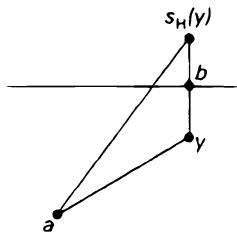
\includegraphics[keepaspectratio]{images/part001_5f5a2798.jpg}}\\
图 1

\begin{enumerate}
\def\labelenumi{(\roman{enumi})}
\setcounter{enumi}{1}
\item
设 \(\mathbf{C}'\) 是一个室且 \(a' \in \mathbf{C}'\)。由已证结果，存在 \(w \in \mathrm{W}_{\mathfrak{M}}\)，使得 \(w^{-1}(a') \in \overline{\mathbf{C}}\)；因此，室 \(\mathbf{C}'\) 与 \(\overline{w(\mathbf{C})}\) 相交；由于 \(\overline{w(\mathbf{C})}\) 是 \(w(\mathbf{C})\) 与内部为空的面片的并（《一般拓扑》第 §1 第 2 号命题 3），故 \(\mathbf{C}' = w(\mathbf{C})\)。
\item
我们必须证明 \(W = W_{\mathfrak{M}}\)，为此只需证明 \(s_{H'} \in W_{\mathfrak{M}}\) 对所有 \(H' \in \mathfrak{H}\) 成立。现在，\(H'\) 至少是一个室 \(C'\) 的墙（《一般拓扑》第 §1 第 4 号命题 8）；我们已经看到，存在 \(w \in W_{\mathfrak{M}}\) 使 \(C' = w(C)\)；于是存在一个墙 \(H\) 属于 \(C\)，使 \(H' = w(H)\)，从而 \(s_{H'} = w.s_H.w^{-1} \in W_{\mathfrak{M}}\)。
\end{enumerate}

\subsection{与 Coxeter 系统的关系}

定理 1. 设 \(\mathbf{C}\) 是一个室，令 \(\mathbf{S}\) 为关于 \(\mathbf{C}\) 的墙的反射所成的集合。

\begin{enumerate}
\def\labelenumi{(\roman{enumi})}
\item
有序对 \((\mathbf{W},\mathbf{S})\) 是一个 Coxeter 系统。
\item
设 \(w \in \mathrm{W}\)，且 \(\mathrm{H}\) 是 \(\mathrm{C}\) 的墙。关系 \(l(s_{\mathrm{H}}w) > l(w)\) 蕴含室 \(\mathrm{C}\) 与 \(w(\mathrm{C})\) 位于 \(\mathrm{H}\) 的同一侧。
\item
对于任意室 \(\mathbf{C}'\)，存在唯一的 \(w \in \mathbf{W}\)，使得 \(w(\mathbf{C}) = \mathbf{C}'\)。
\item
满足 \(\mathbf{H}\) 的超平面 \(s_{\mathrm{H}} \in \mathbf{W}\) 的集合等于 \(\mathfrak{H}\)。
\end{enumerate}

S 的每个元素的阶都是 2，而引理 2 表明 S 生成 W。对于 C 的任一墙 H，记 \(P_{H}\) 为满足下列条件的 \(w \in W\) 所成的集合：室 C 与 \(w(\mathrm{C})\)（它们不与 H 相交）位于 H 的同一侧。我们将验证《代数》第 IV 章 §1 第 7 号的 \((\mathrm{A}')\)、\((\mathrm{B}')\) 和 (C) 条件。

\((A') 1 \in P_H\)：显然。

(B') \(P_{H}\) 与 \(s_{H}.P_{H}\) 不相交：事实上，\(w(\mathrm{C})\) 和 \(s_{H}w(\mathrm{C})\) 位于 H 的相反两侧；因此，若 \(w(\mathrm{C})\) 与 C 在 H 的同一侧，它就不会与 \(s_{\mathrm{H}}w(\mathrm{C})\) 在同一侧。

\begin{enumerate}
\def\labelenumi{(\Alph{enumi})}
\setcounter{enumi}{2}
\tightlist
\item
设 \(w \in \mathrm{P_H}\)，且 \(\mathrm{H}'\) 是 \(\mathbf{C}\) 的一面墙，使 \(ws_{\mathrm{H}'} \notin \mathrm{P_H}\)；则 \(ws_{\mathrm{H}'} = s_{\mathrm{H}}w\)：根据假设，\(w(\mathbf{C})\) 与 \(\mathbf{H}\) 在 \(\mathbf{C}\) 的同一侧，而 \(ws_{\mathrm{H}'}(\mathbf{C})\) 在另一侧。因此，\(ws_{\mathrm{H}'}(\mathbf{C})\) 与 \(w(\mathbf{C})\) 位于 H 的相反两侧；所以，\(s_{\mathrm{H}^{\prime}}(\mathrm{C})\) 与 C 位于超平面 \(w^{-1}(\mathrm{H})\) 的相反两侧。令 a 为支撑为 \(H^{\prime}\) 的 C 的一个面上的点。点 \(a = s_{\mathrm{H}^{\prime}}(a)\) 同时属于室 C 与 \(s_{\mathrm{H}^{\prime}}(\mathrm{C})\) 的闭包，而这两个室分别包含于 \(w^{-1}(\mathrm{H})\) 所界定的两个开半空间中；于是 \(a \in w^{-1}(\mathrm{H})\)，故 \(\mathrm{H}^{\prime} = w^{-1}(\mathrm{H})\)。由此推出 \(s_{\mathrm{H}^{\prime}} = w^{-1}s_{\mathrm{H}}w\)，从而 \(ws_{H^{\prime}} = s_{H}w\)。
\end{enumerate}

断言 (i) 和 (ii) 由此以及《代数》第 IV 章 §1 第 7 号命题 6 得出。此外，我们有（同上，条件 (A)）

\[
\bigcap_ {H \in \mathfrak {M}} P _ {H} = \{1 \}.\tag{3}
\]

引理 2 表明 W 在室的集合上传递。此外，若 \(w \in W\) 满足 \(w(\mathrm{C}) = \mathrm{C}\)，则对 C 的每一面墙 H 都有 \(w \in P_{H}\)，因而由 (3) 得 w = 1。这证明了 (iii)。

最后，设 H 是满足 \(s_{H} \in W\) 的一个超平面。如果 H 不属于 H，则至少存在一个与 H 相交的室 \(C'\)（\(\S1\)，第 3 号命题 7）。\(H \cap C'\) 中的每个交点都在 \(s_{H}\) 作用下不变，因而同时属于室 \(C'\) 和 \(s_{\mathrm{H}}(\mathrm{C}')\)；所以，\(\mathrm{C}' = s_{\mathrm{H}}(\mathrm{C}')\)，这与 (iii) 矛盾，因为 \(s_{H} \neq 1\)。

推论. 设 \(\Sigma\) 是生成 W 的一组反射。那么属于 W 的每个反射都与 \(\Sigma\) 中的一个元素共轭。

令 \(\mathfrak{H}'\) 为形如 \(w(\mathrm{H})\) 的超平面所成的集合，其中 \(w \in \mathrm{W}\)、\(\mathrm{H} \in \mathfrak{H}\)，且 \(s_{\mathrm{H}} \in \Sigma\)。由于 \(\mathrm{W}\) 由族 \((s_{\mathrm{H}})_{\mathrm{H} \in \mathfrak{H}'}\) 生成，且 \(\mathfrak{H}'\) 在 \(\mathrm{W}\) 下稳定，我们可以用 \(\mathfrak{H}'\) 代替 \(\mathfrak{H}\) 应用本号的全部结果；但是定理 1(iv) 表明 \(\mathrm{W}\) 中的每个反射都形如 \(s_{\mathrm{H}}\)，其中 \(\mathrm{H} \in \mathfrak{H}'\)，因此推论得证。

\subsection{基本域与稳定子群}

回顾《积分》第 VII 章 §2 第 10 号定义 2：若 E 的子集 D 使 W 在 E 中的每个轨道都恰好与 D 相交于一点，则称 D 是群 W 的基本域。这等价于下列两个条件：

\begin{enumerate}
\def\labelenumi{\alph{enumi})}
\item
对于每个 \(x \in \mathrm{E}\)，存在 \(w \in \mathrm{W}\)，使得 \(w(x) \in \mathrm{D}\)。
\item
若 \(x, y \in D\) 且 \(w \in W\) 满足 \(y = w(x)\)，则 y = x（即使 \(w \neq 1\)）。
\end{enumerate}

我们将证明下列三个命题：

定理 2. 对任意室 C，C 的闭包 \(\overline{\mathbf{C}}\) 是 W 在 E 上作用的一个基本域。

命题 1. 设 \(\mathbf{F}\) 是一个面片，\(\mathbf{C}\) 是满足 \(\mathbf{F} \subset \overline{\mathbf{C}}\) 的室。设 \(w \in W\)。下列条件等价：

\begin{enumerate}
\def\labelenumi{(\roman{enumi})}
\item
\(w(\mathbf{F})\) 与 F 相交；
\item
\(w(\mathbf{F}) = \mathbf{F};\)
\item
\(w(\overline{\mathrm{F}}) = \overline{\mathrm{F}};\)
\item
w 至少固定 F 中的一个点；
\item
w 固定 F 的每一个点；
\item
w 固定 \(\overline{\mathbf{F}}\) 的每一个点；
\item
w 属于 W 中由包含 F 的 C 的墙的反射生成的子群。
\end{enumerate}

对于 E 的每个子集 A，记 \(W(A)\) 为 W 中由固定 A 的每一个点的元素所成的子群。

命题 2. 设 A 是 E 的非空子集，令 \(\mathfrak{H}_{\mathrm{A}}\) 为包含 A 的超平面 \(\mathrm{H} \in \mathfrak{H}\) 所成的集合，令 \(\mathrm{A}'\) 为这些 \(\mathrm{H} \in \mathfrak{H}_{\mathrm{A}}\) 的交，并令 F 为 E 中在 \(\mathrm{A}'\) 内部开着的一个面片（§1，第 3 号，命题 7）。则 \(\mathrm{W(A)} = \mathrm{W(A')} = \mathrm{W(F)}\)，且 \(\mathrm{W(A)}\) 由关于 \(\mathfrak{H}_{\mathrm{A}}\) 中超平面的反射生成。

我们先证明下列断言：

\begin{enumerate}
\def\labelenumi{(\Roman{enumi})}
\tightlist
\item
设 C 是一个室，设 x 和 y 是 \(\overline{C}\) 中的两个点，并设 \(w \in W\) 满足 \(w(x) = y\)。则 x = y，且 w 属于子群 \(W_{N}\)，其中 N 是包含 x 的 C 的墙的集合。
\end{enumerate}

我们对长度 \(q\) 的 \(w\)（相对于集合 \(S\)（由关于 \(C\) 的墙的反射组成））作归纳，\(q = 0\) 时结论显然。若 \(q \geqslant 1\)，则存在 \(H\) 为 \(C\) 的一个墙以及元素 \(w' \in W\)，使得 \(w = s_H w'\) 且 \(l(w') = q - 1\)。由于 \(l(s_H w) < l(w)\)，根据第 2 号的定理 1，室 \(C\) 与 \(w(C)\) 位于 \(H\) 的相反两侧。因此，\(\overline{C} \cap w(\overline{C}) \subset H\)，所以 \(y \in H\)。于是 \(y = w'(x)\)，归纳假设推出 \(x = y\) 且 \(w' \in W_{\mathfrak{N}}\)。由于 \(y \in H\)，可知 \(H \in \mathfrak{N}\)，从而 \(w = s_H w' \in W_{\mathfrak{N}}\)，(I) 的证明完成。

定理 2 的证明：这由 (I) 和引理 2 得出。

命题 1 的证明：我们知道两个不同的面片不相交且闭包不同（§1，第 2 号，命题 3 的推论）。因此 (i)、(ii)、(iii) 等价。另一方面，显然

\[
(\mathrm{vii}) \Longrightarrow (\mathrm{vi}) \Longrightarrow (\mathrm{v}) \Longrightarrow (\mathrm{iv}) \Longrightarrow (\mathrm{i})
\]

且断言 (I) 表明 (i) \(\Longrightarrow\) (vii)。

命题 2 的证明：令 \(\mathbf{A}''\) 为由 A 生成的 \(\mathbf{E}\) 的仿射子空间。显然，\(\mathrm{W(A)} = \mathrm{W(A'')}\)。由 §1 第 3 号的命题 7，存在点 \(x \in \mathbf{A}''\)，它不属于任何超平面 \(\mathbf{H} \in \mathfrak{H} - \mathfrak{H}_{\mathbf{A}}\)。令 \(\mathbf{F}_x\) 为包含 \(x\) 的面片：它在 \(\mathbf{A}''\) 中是开的，而命题 1 表明

\[
\mathrm{W} \left(\mathrm{F} _ {x}\right) \subset \mathrm{W} \left(\mathrm{A} ^ {\prime}\right) \subset \mathrm{W} (\mathrm{A}) = \mathrm{W} \left(\mathrm{A} ^ {\prime \prime}\right) \subset \mathrm{W} (\{x \}) = \mathrm{W} \left(\mathrm{F} _ {x}\right),
\]

从而 \(\mathrm{W(A) = W(A') = W(F_x)}\)。将 A 替换为 F，我们也有

\[
\mathrm{W} (\mathrm{A}) = \mathrm{W} (\mathrm{F}),
\]

因此命题得证。

注. 1) 由定理 2 可知，若 C 是一个室而 F 是一个面片，则存在唯一的面片 \(F'\) 包含于 \(\overline{C}\)，它被 W 的一个元素变换为 F。

\begin{enumerate}
\def\labelenumi{\arabic{enumi})}
\setcounter{enumi}{1}
\item
由命题 1 和 2 可知，对于 E 的任意非空子集 A，存在一点 \(a \in E\)，使得 \(W(A) = W(\{a\})\)；此外，群 \(W(A)\) 是一个 Coxeter 群（定理 1）。
\item
设 \(\mathbf{C}\) 是 \(\mathbf{E}\) 的一个室，\(\mathbf{S}\) 是关于 \(\mathbf{C}\) 的墙的反射所成的集合。设 \(w \in W\)，并设 \((s_1, \ldots, s_q)\) 是 \(w\) 关于 \(\mathbf{S}\) 的一个约化分解。若 \(x \in \overline{\mathbf{C}}\) 被 \(w\) 固定，则有 \(s_j(x) = x\) 对所有 \(j\) 成立：这由上述命题 1 以及《代数》第 IV 章 §1 的命题 7 的推论 1 得出。
\end{enumerate}

\subsection{W 的 Coxeter 矩阵与 Coxeter 图}

设 C 是一个室，\(S = S(C)\) 为关于 C 的墙的正交反射所成的集合，\(M = (m(s, s'))\) 为 Coxeter 系统 (W, S) 的 Coxeter 矩阵（《代数》第 IV 章 §1 第 9 号）；回顾 \(m(s, s')\) 是 W 中元素 \(ss'\) 的阶（有限或无限）（其中 \(s, s' \in S\)）。若 \(C'\) 是另一个室，则满足 \(w \in W\) 且 \(w(C) = C'\) 的唯一元素 w 定义一个双射

\[
s \mapsto f (s) = w s w ^ {- 1}
\]

从 S 到 \(S' = S(C')\)，并且有 \(m(f(s), f(s')) = m(s, s')\)。由此，如果 W 通过 \((C, s)\) 作用于由二元组 \(s \in S(C)\) 构成的集合 X，其中 C 是一个室且 \(w.(C, s) = (w(C), wsw^{-1})\)，则 W 在 X 中的每个轨道都与集合 \(\{C\} \times S(C)\) 恰好相交于一点，我们记该点为 \((C, s_i(C))\)。因此，若 I 是轨道集且 \(i, j \in I\)，数值 \(m_{ij} = m(s_i(C), s_j(C))\) 与室 C 的选择无关。矩阵 \(M(W) = (m_{ij})_{i,j \in I}\) 是一个 Coxeter 矩阵，称为 W 的 Coxeter 矩阵。与 M(W) 相关的 Coxeter 图（《代数》第 IV 章 §1 第 9 号）称为 W 的 Coxeter 图。

设 C 是一个室。对于任意 \(i \in I\)，记 \(\mathrm{H}_{i}(\mathrm{C})\) 为 C 的满足下述条件的墙：\(s_{i}(\mathrm{C})\) 是关于 \(\mathrm{H}_{i}(\mathrm{C})\) 的反射；并记 \(e_{i}(\mathrm{C})\) 为与 \(\mathrm{H}_{i}(\mathrm{C})\) 正交、且位于 \(\mathrm{H}_{i}(\mathrm{C})\) 与 C 同一侧的单位向量。映射 \(i \mapsto \mathrm{H}_{i}(\mathrm{C})\) 称为 C 的规范编号墙族。

命题 3. 设 \(\mathbf{C}\) 是一个室，且 \(i, j \in \mathbf{I}\) 满足 \(i \neq j\)。置 \(s_i = s_i(\mathbf{C})\)、\(\mathbf{H}_i = \mathbf{H}_i(\mathbf{C})\)、\(e_i = e_i(\mathbf{C})\)，并类似地定义 \(s_j\)、\(\mathbf{H}_j\) 和 \(e_j\)。

\begin{enumerate}
\def\labelenumi{(\roman{enumi})}
\item
若 \(\mathrm{H}_i\) 与 \(\mathrm{H}_j\) 平行，则 \(m_{ij} = \infty\) 且 \(e_i = -e_j\)。
\item
若 \(\mathrm{H}_i\) 与 \(\mathrm{H}_j\) 不平行，则 \(m_{ij}\) 有限，且
\end{enumerate}

\[
\left(e _ {i} \mid e _ {j}\right) = - \cos (\pi / m _ {i j}).\tag{4}
\]

\begin{enumerate}
\def\labelenumi{(\roman{enumi})}
\setcounter{enumi}{2}
\tightlist
\item
有 \((e_i|e_j)\leqslant 0\)。
\end{enumerate}

若 \(\mathrm{H}_i\) 与 \(\mathrm{H}_j\) 平行，则 \(s_i s_j\) 是一个平移（§2，第 4 号，命题 5），所以 \(m_{ij} = \infty\)。此外，或者 \(e_i = e_j\)，或者 \(e_i = -e_j\)。现在，闭包 C 中存在一点 \(a\)（分别为 \(a'\)），它属于 \(\mathrm{H}_i\)（分别属于 \(\mathrm{H}_j\)），但不属于 \(\mathrm{H}_j\) \((\text{resp. } \mathrm{H}_i)\)。于是 \((a' - a|e_i) > 0\) 且 \((a - a'|e_j) > 0\)，这排除了 \(e_i = e_j\) 的情形，并证明了 (i)。

现在假设 \(H_{i}\) 与 \(H_{j}\) 不平行。取 \(a \in H_{i} \cap H_{j}\) 为原点，并通过双射 \(t \mapsto a + t\) 将 T 与 E 识别。令 V 为与 \(H_{i} \cap H_{j}\) 正交且经过 a 的平面。置 \(\Gamma = V \cap D_{H_{i}}(C) \cap D_{H_{j}}(C)\)（其中 \(D_{H}(C)\) 表示由 H 界定且包含 C 的开半空间（§1，第 1 号）），并令 D（分别为 \(D'\)）为 V 中包含于 \(H_{i} \cap V\)（分别为 \(H_{j} \cap V\)）且包含于 \(\Gamma\) 闭包中的半直线。对 V 取适当的定向后，集合 \(\Gamma\) 是 V 中满足下式的开半直线 \(\Delta\) 的并：

\[
0 <   (\widehat {\mathrm{D} , \Delta}) <   (\widehat {\mathrm{D} , \mathrm{D} ^ {\prime}}).
\]

令 \(W'\) 为由 \(W\) 和 \(s_i\) 生成的 \(s_j\) 的子群。对于任意 \(w \in W'\)，超平面 \(w(H_i)\) 和 \(w(H_j)\) 属于 \(\mathfrak{H}\)，包含 \(H_i \cap H_j\)，且不与 C 相交。因此，它们不与 \(\Gamma\) 相交（§1，第 5 号，命题 10）。于是，§2 第 5 号命题 7 的推论蕴含 (ii)。

最后，断言 (iii) 直接由 (i) 和 (ii) 得出，因为 \(m_{ij} \geqslant 2\) 对 \(i \neq j\) 成立。

注. 公式 (4) 实际上对所有 \(i, j \in I\) 都成立：事实上，当 \(\pi / m_{ij} = 0\) 时，\(m_{ij} = \infty\)，而当 \(i = j\) 时，\(m_{ij} = 1\) 且 \((e_i | e_j) = 1\)。

\subsection{标量积为负的向量系}

引理 3. 设 \(q\) 是实向量空间 \(V\) 上的一个正二次型，\(B\) 是与之关联的对称双线性型。设 \(a_1, \ldots, a_n\) 是 \(V\) 中满足 \(B(a_i, a_j) \leqslant 0\) 对 \(i \neq j\) 的元素。

\begin{enumerate}
\def\labelenumi{(\roman{enumi})}
\tightlist
\item
若 \(c_{1}, \ldots, c_{n}\) 是满足 \(q\left(\sum_{i} c_{i} a_{i}\right) = 0\) 的实数，则
\end{enumerate}

\[
q \left(\sum_ {i} | c _ {i} | a _ {i}\right) = 0.
\]

\begin{enumerate}
\def\labelenumi{(\roman{enumi})}
\setcounter{enumi}{1}
\tightlist
\item
若 \(q\) 非退化，且存在 \(f\) 上的线性形式 \(V\)，使得 \(f(a_i) > 0\) 对所有 \(i\) 成立，则向量 \(a_1, \ldots, a_n\) 线性无关。
\end{enumerate}

关系 \(\mathrm{B}(a_i, a_j) \leqslant 0\) 对 \(i \neq j\) 立即推出

\[
q \left(\sum_ {i} | c _ {i} | a _ {i}\right) \leqslant q \left(\sum_ {i} c _ {i} a _ {i}\right),
\]

若 \(q\) 非退化，则关系 \(\sum_{i} c_{i} a_{i} = 0\) 从而蕴含

\[
\sum_ {i} | c _ {i} | a _ {i} = 0;
\]

于是，对于 \(f\) 上的任意线性形式 \(\mathbf{V}\)，有 \(\sum_{i}|c_i|f(a_i) = 0\)，从而 \(c_i = 0\) 对所有 \(i\) 成立，条件是还对所有 \(f(a_i) > 0\) 有 \(i\)。这证明了 (ii)。

引理 4. 设 \(\mathbf{Q} = (q_{ij})\) 是一个实的、对称的、\(n\) 阶方阵，满足：

\begin{enumerate}
\def\labelenumi{\alph{enumi})}
\item
  \(q_{ij} \leqslant 0\) for \(i \neq j\) ;
\item
不存在将 \(\{1,2,\ldots,n\}\) 划分为两个非空子集 I 和 J 的划分，使得 \((i,j)\in\mathrm{I}\times\mathrm{J}\) 蕴含 \(q_{ij}=0\)；
\item
二次型 \(q(x_{1},\ldots ,x_{n}) = \sum_{i,j}q_{ij}x_{i}x_{j}\) 定义在 \(\mathbf{R}^n\) 上且为正。
\end{enumerate}

于是：

\begin{enumerate}
\def\labelenumi{(\roman{enumi})}
\item
\(\mathbf{N}\) 是 \(q\) 的核，其维数为 0 或 1。若 \(\dim \mathbf{N} = 1\)，则 \(\mathbf{N}\) 由一个所有坐标均 \(> 0\) 的向量生成。
\item
\(\mathbf{Q}\) 的最小特征值的重数为 1，并且相应的特征向量的所有坐标均 \(>0\) 或均 \(< 0\)。
\end{enumerate}

由于 \(q\) 是正二次型，\(N\) 是 \(q\) 的迷向向量集合（关于 \(q\) 而言）（《代数》第 IX 章 §7 第 1 号命题 2 的推论）。令 \(a_1, \ldots, a_n\) 为 \(\mathbf{R}^n\) 的标准基。若 \(\sum_{i} c_i a_i \in N\)，引理 3 表明 \(\sum_{i} |c_i| a_i \in N\) 也成立，从而有 \(\sum_{i} q_{ji}|c_i| = 0\) 对所有 \(j\) 成立。令 \(I\) 为 \(i\) 满足 \(c_i \neq 0\) 时的指标集合。若 \(j \notin I\)，则 \(q_{ji}|c_i| \leqslant 0\) 对 \(i \in I\) 成立，而 \(q_{ji}|c_i| = 0\) 对 \(i \notin I\) 成立，所以 \(q_{ji} = 0\) 对 \(j \notin I\) 且 \(i \in I\) 成立。因此，假设 \(b)\) 蕴含 \(I = \varnothing\) 或 \(I = \{1, \ldots, n\}\)。于是，\(N\) 中每个非零向量的所有坐标都 \(\neq 0\)。若 \(\dim N \geqslant 2\)，则 \(N\) 与方程为 \(x_i = 0\) 的超平面的交的维数将 \(\geqslant 1\)，这与我们刚才证明的事实矛盾。前面的论证还表明，若 \(\dim N = 1\)，则 \(N\) 含有一个所有坐标均 \(>0\) 的向量。这证明了 (i)。

另一方面，我们知道 Q 的特征值为实数（《代数》第 IX 章 §7 第 3 号命题 5），且由于 q 为正的而为正。令 \(\lambda\) 为其中最小者。矩阵 \(Q' = Q - \lambda I_n\) 是退化正型 \(q'\) 的矩阵，而 \(Q'\) 的非对角元素与 Q 的相同。因此，\(Q'\) 满足本引理陈述中的条件 a)、b) 和 c)。由于 \(N'\) 是 \(q'\) 的核，且是 Q 对应于特征值 \(\lambda\) 的特征子空间，断言 (ii) 由 (i) 得出。

引理 5. 设 \(e_1, \ldots, e_n\) 是生成 \(T\) 的向量，满足：

\(a) (e_i | e_j) \leqslant 0 \text{ 当 } i \neq j;\)

\begin{enumerate}
\def\labelenumi{\alph{enumi})}
\setcounter{enumi}{1}
\tightlist
\item
不存在将 \(\{1, \ldots, n\}\) 划分为两个非空子集 I 和 J 的划分，使得 \((e_i|e_j) = 0\) 对 \(i \in I\) 且 \(j \in J\) 成立。
\end{enumerate}

于是有两种可能：

\begin{enumerate}
\def\labelenumi{\arabic{enumi})}
\item
\((e_1, \ldots, e_n)\) 是 T 的一个基；
\item
\(n = \dim T + 1\)；存在一个族 \((c_i)_{1 \leqslant i \leqslant n}\)，其元素为 \(> 0\) 的实数，并满足 \(\sum_{i} c_i e_i = 0\)，并且任何实数族 \((c_i')_{1 \leqslant i \leqslant n}\) 满足 \(\sum_{i} c_i' e_i = 0\) 时，都与 \((c_i)_{1 \leqslant i \leqslant n}\) 成比例。
\end{enumerate}

置 \(q_{ij} = (e_i|e_j)\)。于是矩阵 \(Q = (q_{ij})\) 满足引理 4 的假设：引理 4 的条件 a) 和 b) 分别就是上述条件 a) 和 b)，而 c) 得到满足，因为 \(\sum_{i,j} q_{ij} x_i x_j = \|\sum_{i} x_i e_i\|^2\)。\(q\) 在 \(\mathbf{R}^n\) 上且矩阵为 \(\mathbf{Q}\) 的二次型的核 N，是 \((c_1, \ldots, c_n) \in \mathbf{R}^n\) 中满足 \(\sum_{i} c_i e_i = 0\) 的向量所成的集合。若 \(N = \{0\}\)，则 \(e_i\) 线性相关，我们处于情形 1)。若 \(\dim N > 0\)，引理 4(i) 表明我们处于情形 2)。

引理 6. 设 \((e_1, \ldots, e_n)\) 是 T 的一个基，且 \((e_i | e_j) \leqslant 0\) 对 \(i \neq j\) 成立。

\begin{enumerate}
\def\labelenumi{(\roman{enumi})}
\item
若 \(x = \sum_{i} c_i e_i \in \mathbf{T}\) 满足 \((x|e_i) \geqslant 0\) 对所有 \(i\) 成立，则 \(c_i \geqslant 0\) 对所有 \(i\) 成立。
\item
若 \(x\) 和 \(y\) 是 \(\mathrm{T}\) 中的两个元素，满足 \((x|e_i) \geqslant 0\) 且 \((y|e_i) \geqslant 0\) 对所有 \(i\) 成立，则 \((x|y) \geqslant 0\)。若 \((x|e_i) > 0\) 且 \((y|e_i) > 0\) 对所有 \(i\) 成立，则 \((x|y) > 0\)。
\end{enumerate}

在 (i) 的假设下，假设某个 \(c_{i} < 0\)，其中 \(i\) 为固定指标。令 \(f\) 为 \(T\) 上由 \(f(e_{i}) = 1\) 定义的线性形式，并且

\[
f \left(e _ {j}\right) = - c _ {i} / \left(\sum_ {k = 1} ^ {n} \left| c _ {k} \right|\right) \quad \text { for } j \neq i.
\]

于是，向量 \(-x, e_1, \ldots, e_n\) 满足引理 3(ii) 的假设（取 T 上的度量型作为 \(q\)）。我们得到它们线性无关，这不可能。因此 (i) 成立。此外，若 \(x = \sum_{i} c_i e_i \in \mathbf{T}\) 且 \(y \in \mathbf{T}\)，则 \((x|y) = \sum_{i} c_i (e_i | y)\)，所以 (ii) 立即由 (i) 得出。

\subsection{有限性定理}

引理 7. 设 A 是 T 中的单位向量集。若存在实数 \(\lambda < 1\)，使得 \((a|a') \leqslant \lambda\) 对于 \(a, a' \in \mathbf{A}\) 且 \(a \neq a'\) 成立，则 A 是有限集。

对于 \(a, a' \in A\) 且 \(a \neq a'\)，有

\[
\left\| a - a ^ {\prime} \right\| ^ {2} = 2 - 2 (a \mid a ^ {\prime}) \geqslant 2 - 2 \lambda .
\]

现在，T 的单位球面 S 是紧的，因此存在一个由直径 \(<(2-2\lambda)^{1/2}\) 的集合组成的有限覆盖，并且这些集合中每个至多包含 A 的一个点，于是引理得证。

记 \(U(w)\) 为与从 E 到自身的仿射映射 \(w \in W\) 相关联的 T 的自同构。我们有

\[
w (x + t) = w (x) + \operatorname{U} (w). t \text {for} t \in \mathrm{T} \text {and} x \in \mathrm{E}.
\]

这定义了从群 W 到 T 的正交群的同态 U；U 的核是属于 W 的平移。

定理 3. (i) 一个室的墙的集合是有限的。

\begin{enumerate}
\def\labelenumi{(\roman{enumi})}
\setcounter{enumi}{1}
\item
属于 \(\mathfrak{H}\) 的超平面的方向的集合是有限的。
\item
群 U(W) 是有限的。
\end{enumerate}

断言 (i) 立即由命题 3(iii) 和引理 7 得出。

设 \(\mathbf{C}\) 是一个室，\(\mathfrak{M}\) 是其墙的集合。\(\overline{\mathbf{C}}\) 的面片（相对于 \(\mathfrak{H}\)）与相对于 \(\mathfrak{M}\) 的相同（§ 1，第 4 号，命题 9）。

由于 M 是有限的，面片的数目也是有限的。由于一个面片只与有限个属于 H 的超平面相交，所以与 \(\overline{C}\) 相交的属于 H 的超平面集合是有限的，因而 A(C)（即与某个属于 H 且与 \(\overline{C}\) 相交的超平面正交的 T 中单位向量的集合）也是有限的。因此，存在实数 \(\lambda < 1\)，使得 \((a|a') \leqslant \lambda\) 对于 \(a, a' \in A(C)\) 且 \(a \neq a'\) 成立。

令 A 为与属于 H 的某个超平面正交的 T 中单位向量所成的集合。设 \(a, a' \in A\) 且 \(a \neq a'\)。若 a 与 \(a'\) 平行，则 \(a = -a'\) 且 \((a|a') = -1\)。否则，令 \(H \in H\)（分别为 \(H' \in H\)）满足 a（分别为 \(a'\)）与 H（分别与 \(H'\)）正交。我们有 \(H \cap H' \neq \varnothing\)，且若 \(x \in H \cap H'\)，则存在元素 \(w \in W\)，使得 \(x \in w(\overline{C})\)。于是，向量 \(U(w).a\) 和 \(U(w).a'\) 属于 A(C)，且有

\[
(a \mid a ^ {\prime}) = (\mathrm{U} (w). a \mid \mathrm{U} (w). a ^ {\prime}) \leqslant \lambda ,
\]

且由引理 7，集合 \(\mathbf{A}\) 是有限的。因此 (ii)。

现在，设 \(w \in W\)，满足 \(\mathrm{U}(w).a = a\) 对所有 \(a \in A\) 成立。则 \(\mathrm{U}(w).t = t\) 对 T 中由 A 生成的子空间内的所有 t 成立。另一方面，若 \(t \in T\) 与 A 正交，则对所有 \(\mathrm{U}(s_{\mathrm{H}}).t = t\) 都有 \(H \in H\)，因而 \(\mathrm{U}(w).t = t\)，最终 \(\mathrm{U}(w) = 1\)。由于对所有 \(\mathrm{U}(w)(\mathrm{A}) = \mathrm{A}\) 都有 \(w \in W\)，我们得到 \(\mathrm{U}(\mathrm{W})\) 同构于有限集 A 的一个置换群，因此 (iii)。

命题 4. 设 C 是一个室，N 是 C 的一组墙。令 \(W_{N}\) 为由关于 N 中元素的正交反射生成的 W 的子群。对于 \(H \in N\)，记 \(e_{H}\) 为与 H 正交且位于 H 与 C 同一侧的单位向量。下列条件等价：

\begin{enumerate}
\def\labelenumi{(\roman{enumi})}
\item
群 \(\mathbf{W}_{\mathfrak{N}}\) 是有限的。
\item
存在 \(\mathbf{E}\) 中一点，在 \(W_{\mathfrak{N}}\) 的每个元素下不变。
\item
属于 \(\mathfrak{N}\) 的超平面有非空交。
\item
向量族 \((e_{\mathrm{H}})_{\mathrm{H}\in \mathfrak{N}}\) 在 T 中自由。
\end{enumerate}

根据 §3 开头的性质 (D2)，W 中每一点的稳定子都是有限的，因此 (ii) 蕴含 (i)。

由于群 \(W_{N}\) 由关于属于 N 的超平面所成的反射集合生成，\(W_{N}\) 的不动点就是属于每个超平面 \(H \in N\) 的 E 中的点，因此 (ii) 与 (iii) 等价。

假设 \(a\) 是 \(E\) 中的一点，使得 \(a \in H\) 对所有 \(H \in \mathfrak{N}\) 成立，并令 \(t \in T\) 满足 \(a + t \in C\)。由于 \((e_H | e_{H'}) \leqslant 0\) 对满足 \(H, H' \in \mathfrak{N}\) 且 \(H \neq H'\) 的情形成立（命题 3），又由于 \((t | e_H) > 0\) 对所有 \(H \in \mathfrak{N}\) 成立，引理 3(ii) 蕴含 \(e_H\)（其中 \(H \in \mathfrak{N}\)）线性无关。因此，(iii) 蕴含 (iv)。

最后，假设向量族 \((e_{\mathrm{H}})_{\mathrm{H}\in\mathfrak{N}}\) 是自由的。令 a 为 E 中一点。对于任意 \(H\in N\)，存在实数 \(c_{H}\)，使得 H 恰好由 E 中满足 \(a+t\) 的点 \((t|e_{\mathrm{H}})=c_{\mathrm{H}}\) 组成。由于族 \((e_{\mathrm{H}})\) 是自由的，存在 \(t\in T\)，使得 \((t|e_{\mathrm{H}})=c_{\mathrm{H}}\) 对所有 \(H\in N\) 成立，且 E 中的点 \(a+t\) 属于所有超平面 \(H\in N\)。因此，(iv) 蕴含 (iii)。

注. 1) 由于 W 由关于室 C 的墙的反射生成，前一命题给出了 W 有限的一个判据。我们将在第 9 号回到这个问题。

\begin{enumerate}
\def\labelenumi{\arabic{enumi})}
\setcounter{enumi}{1}
\tightlist
\item
设 F 是有限维实仿射空间，G 是 F 的自同构群。对于所有 \(g \in G\)，记 \(U(g)\) 为与 g 相关的 F 的平移空间 V 的自同构。假设 \(U(G)\) 的像是 \(\mathbf{GL}(V)\) 的有限子群；则 V 具有一个在 \(U(G)\) 下不变的标量积（《积分》第 VII 章 §3 第 1 号命题 1）。此外，如果 G 配备离散拓扑后在 F 上适当地作用，且由反射生成，则可以将本段的结果应用于 G。
\end{enumerate}

\subsection{W 在 T 上的线性表示的分解}

令 I 为 W 的 Coxeter 图的顶点集（第 4 号），令 J 为 I 的一个子集，使 J 中没有顶点与 I-J 中的任何顶点相连。设 C 是一个室，s 是从 I 到关于 C 的墙的反射集合的规范双射，并令 \(W_{J,C}\) 为由像 \(s(\mathrm{J})\) 生成的子群。由《代数》第 IV 章 §1 第 9 号命题 8 可知，W 是两个子群 \(W_{J,C}\) 和 \(W_{I-J,C}\) 的直积。设 \(C'\) 是另一个室，\(s'\) 是从 I 到 W 的相应单射。我们已经看到（第 4 号），若 \(w \in W\) 将 C 变换为 \(C'\)，则有 \(s'(\mathrm{i}) = ws(\mathrm{i})w^{-1}\)，其中 \(i \in I\)。由于 \(W_{J,C}\) 在 W 中正规，可知 \(s'(\mathrm{i}) \in W_{J,C}\) 对所有 \(i \in J\) 成立。我们推得子群 \(W_{J,C}\) 与 C 无关。从现在起将其简记为 \(W_{J}\)。

\(W_{J,C}\) 的定义显然可推广到 I 的任意子集 J。但是，如果 J 中有一个顶点与 I-J 中的一个顶点相连，则 \(W_{J,C}\) 不正规并且取决于 C 的选择。

令 \(T_{J}^{0}\) 为 T 中在 \(U(W_{J})\) 的每个元素下不变的向量所成的子空间，令 \(T_{J}\) 为与 \(T_{J}^{0}\) 正交的子空间。由于 \(W_{J}\) 是 W 的正规子群，显然 \(T_{J}^{0}\) 在 \(U(W)\) 下不变，因而 \(T_{J}\) 也是如此。

命题 5. 设 \(J_{1},\ldots,J_{s}\) 是 W 的 Coxeter 图的连通分支的顶点集。对于 \(1\leqslant p\leqslant s\)，置

\[
\mathrm{W} _ {p} = \mathrm{W} _ {\mathrm{J} _ {p}}, \quad \mathrm{T} _ {p} = \mathrm{T} _ {\mathrm{J} _ {p}}; \quad \mathrm{T} _ {p} ^ {\prime} = \mathrm{T} _ {\mathrm{J} _ {p}} ^ {0}, \quad \text {and} \quad \mathrm{T} _ {0} = \bigcap_ {1 \leqslant p \leqslant s} \mathrm{T} _ {p} ^ {\prime}.
\]

\begin{enumerate}
\def\labelenumi{(\roman{enumi})}
\item
群 W 是群 \(\mathrm{W}_p\) 的直积（\(1 \leqslant p \leqslant s\)）。
\item
空间 \(\mathbf{T}\) 是子空间 \(\mathrm{T}_0, \mathrm{T}_1, \ldots, \mathrm{T}_s\) 的正交直和，它们都在 \(\mathrm{U}(\mathrm{W})\) 下稳定。
\item
对于所有 \(q\) 满足 \(1 \leqslant q \leqslant s\)，子空间 \(\mathrm{T}_q'\) 是 \(\mathrm{T}\) 中由在 \(\mathrm{U}(\mathrm{W}_q)\) 的每个元素下不变的向量所成的；它是 \(\mathrm{T}_p\)（\(1 \leqslant p \leqslant s\) 且 \(p \neq q\)）的直和。
\item
设 \(\mathbf{C}\) 是一个室。子空间 \(\mathrm{T}_p\)（\(1 \leqslant p \leqslant s\)）由向量 \(e_i(\mathbf{C})\)（其中 \(i \in \mathrm{J}_p\)）生成（按第 4 号的记号）。
\item
W 在子空间 \(T_{p}\)（\(1 \leqslant p \leqslant s\)）上的表示是绝对不可约、非平凡且两两不等价的。
\end{enumerate}

断言 (i) 由《代数》第 IV 章 §1 第 9 号得出。另一方面，我们已经看到子空间 \(\mathrm{T}_p\) 在 \(\mathrm{U}(\mathrm{W})\) 下不变，\(\mathrm{T}_0\) 也如此。设 \(\mathrm{C}\) 是一个室；由于 \(\mathrm{W}_p\) 由反射 \(s_i(\mathrm{C})\)（其中 \(i \in \mathrm{J}_p\)）生成，显然 \(\mathrm{T}_p'\) 是与 \(e_i(\mathrm{C})\)（其中 \(i \in \mathrm{J}_p\)）正交的子空间，因而得到 (iv)。此外，若 \(i \in \mathrm{J}_p\)、\(j \in \mathrm{J}_q\) 且 \(p \neq q\)，则 \(m_{ij} = 2\)，因为 \(\{i,j\}\) 不是 \(\mathrm{W}\) 的 Coxeter 图的一条边，所以 \((e_i|e_j) = 0\)。断言 (ii) 现已显然。断言 (iii) 则随之得出，因为 \(\mathrm{T}_q'\) 是 \(\mathrm{T}_q\) 的正交补。

最后，设 V 是在 \(T_{p}\) 下不变的 \(\mathrm{U}(\mathrm{W}_{p})\) 的子空间。对于所有 \(i \in J_{p}\)，要么 \(e_{i} \in V\)，要么 \(e_{i}\) 与 V 正交（\(\S2\)2，第 2 号，命题 3）。令 A（分别为 B）为满足 \(i \in J_{p}\)（分别为 \(e_{i} \in V\) 与 V 正交）的 \(e_{i}\) 所成的集合。显然，对 \((e_{i}|e_{j}) = 0\) 且 \(i \in A\) 有 \(j \in B\)，而由于 \(J_{p}\) 连通，可知或者 A = \(\varnothing\) 且 V = \(\{0\}\)，或者 A = \(J_{p}\) 且 V = \(T_{p}\)。因此，\(W_{p}\) 在 \(T_{p}\) 上的表示是不可约的，从而是绝对不可约的（\(\S2\)2，第 1 号，命题 1）。根据 \(T_{p}\) 的定义，它是非平凡的。最后，(v) 中的最后一个断言立即由 (iii) 得出。

如果 T 中在 U(W) 下不变的子空间 \(T_{0}\) 缩减为 \(\{0\}\)，则称 W 是本质的；如果 W 在 T 上的表示 U 是不可约的，则称 W 是不可约的。

推论. 假设 \(W \neq \{1\}\)。则 W 不可约，当且仅当它是本质的且其 Coxeter 图连通。

注. 在命题 5 的假设下，\(T_{p}\)（\(0 \leqslant p \leqslant s\)）是 W 在 T 上的线性表示 U 的等型分量（《代数》第 VIII 章 §3 第 4 号）。由此（同上，命题 11），T 中每个在 W 下稳定的向量子空间 V 都是 \(V \cap T_{p}\)（\(0 \leqslant p \leqslant s\)）之和；此外（同上，命题 10），每个与 \(U(w)\) 的算子 \(w \in W\) 对易的自同态都使每个 \(T_{p}\)（\(0 \leqslant p \leqslant s\)）保持稳定，并且对 \(1 \leqslant p \leqslant s\) 在其上诱导一个仿射伸缩。特别地，T 上在 W 下不变的双线性型 \(\Phi\) 是由下式给出的双线性型

\[
\varPhi \left(\sum_ {k} t _ {k}, \sum_ {k} t _ {k} ^ {\prime}\right) = \varPhi_ {0} (t _ {0}, t _ {0} ^ {\prime}) + \sum_ {1 \leqslant p \leqslant s} a _ {p} (t _ {p} | t _ {p} ^ {\prime}),
\]

其中 \(\Phi_{0}\) 是 \(T_{0}\) 上的双线性型，而 \(a_{p}\)（对 \(1 \leqslant p \leqslant s\)）是一个实数：事实上，这样的型 \(\Phi\) 可以唯一地写成 \((t, t') \mapsto (\mathrm{A}(t)|t')\) 的形式，其中 A 是一个与 \(\mathrm{U}(w)\) 的 \(w \in W\) 对易的 T 的自同态。

\subsection{仿射空间 E 的乘积分解}

我们沿用命题 5 的记号。对于 \(0 \leqslant p \leqslant s\) ，设 \(\mathbf{E}_p\) 为群 \(\mathbf{T}_p'\) 在 \(\mathbf{E}\) 中诸轨道所成的集合，\(\varphi_p\) 为从 \(\mathbf{E}\) 到 \(\mathbf{E}_p\) 的典范映射。\(\mathbf{T}\) 在 \(\mathbf{E}\) 上的作用可过渡到商；特别地，\(\mathbf{T}_p\) 作用于 \(\mathbf{E}_p\) ，并且立即可见（例如在 \(\mathbf{E}\) 中取一个原点），\(\mathbf{E}_p\) 是一个仿射空间，以 \(\mathbf{T}_p\) 为其平移空间。置 \(\mathbf{E}' = \mathbf{E}_0 \times \cdots \times \mathbf{E}_s\) ；这是一个仿射空间，以 \(\mathbf{T} = \mathbf{T}_0 \oplus \cdots \oplus \mathbf{T}_s\) 为其平移空间。设 \(\varphi : \mathbf{E} \to \mathbf{E}'\) 为诸 \(\varphi_p\) 的乘积映射；由于 \(\varphi\) 与 \(\mathbf{T}\) 的作用交换，它是一个双射，甚至是仿射空间的同构。在下文中，我们把 \(\mathbf{E}\) 与 \(\mathbf{E}'\) 依照 \(\varphi\) 等同起来；映射 \(\varphi_p\) 于是等同于 \(\mathbf{E}'\) 到 \(\mathbf{E}_p\) 上的典范投影。

由于 W 保持 \(T_{p}^{\prime}\) 稳定，W 在 E 上的作用过渡到商，并定义 W 在 \(E_{p}\) 上的一个作用（对于 \(0 \leqslant p \leqslant s\) ），从而由限制得到 \(W_{p}\) 在 \(E_{p}\) 上的一个作用（对于 \(1 \leqslant p \leqslant s\) ）。另一方面，设 C 是一个室，\(i \in I\) ，并设 p 是使 \(i \in J_{p}\) 的整数。对于任意 \(x \in E\) ，我们有

\[
s _ {i} (\mathrm{C}) (x) = x - \lambda . e _ {i} (\mathrm{C}) \quad \text { with } \quad \lambda \in \mathbf {R}.
\]

由于 \(e_i \in \mathbf{T}_q'\) （对于 \(q \neq p\) ），由此得到

\[
\varphi_ {q} (w (x)) = \varphi_ {q} (x) \text {for} x \in \mathrm{E}, w \in \mathrm{W} _ {p}; 0 \leqslant q \leqslant s \text {and} q \neq p.
\]

因此，若 \(w = w_{1} \ldots w_{s} \in \mathrm{W}\) ，其中 \(w_{p} \in \mathrm{W}_{p}\) （对于 \(1 \leqslant p \leqslant s\) ），则

\[
w \left(\left(x _ {0}, \dots , x _ {s}\right)\right) = \left(x _ {0}, w _ {1} \left(x _ {1}\right), \dots , w _ {s} \left(x _ {s}\right)\right)\tag{5}
\]

对所有 \(x_{p} \in E_{p}\) （对于 \(0 \leqslant p \leqslant s\) ）成立。换言之，W 在 \(E = E'\) 上的作用恰是诸 \(W_{p}\) 在 \(E_{p}\) 上作用的乘积（我们置 \(W_{0} = \{1\}\) ）。由此可知，\(W_{p}\) 忠实地作用于 \(E_{p}\) ，并且 \(W_{p}\) 可等同于欧氏空间 \(E_{p}\) 的一个位移群（当然，平移空间 \(T_{p}\) —— 即 \(E_{p}\) 的平移空间 —— 赋予由 T 上的标量积所诱导的标量积）。

命题 6. (i) 群 \(W_{p}\) 是欧氏仿射空间 \(E_{p}\) 的一个位移群；它由反射生成；赋予离散拓扑后，它适当地作用于 \(E_{p}\) ；它是不可约的。

\begin{enumerate}
\def\labelenumi{(\roman{enumi})}
\setcounter{enumi}{1}
\tightlist
\item
  设 \(\mathfrak{H}_p\) 为超平面 \(\mathrm{H}\)（在 \(\mathrm{E}_p\) 中且满足 \(s_{\mathrm{H}} \in \mathrm{W}_p\) ）所成的集合。集合 \(\mathfrak{H}\) 由形如
\end{enumerate}

\[
\mathrm{H} = \mathrm{E} _ {0} \times \mathrm{E} _ {1} \times \dots \times \mathrm{E} _ {p - 1} \times \mathrm{H} _ {p} \times \mathrm{E} _ {p + 1} \times \dots \times \mathrm{E} _ {s},
\]

其中 \(p = 1,\dots ,s\) 且 \(\mathrm{H}_p\in \mathfrak{H}_p\)

\begin{enumerate}
\def\labelenumi{(\roman{enumi})}
\setcounter{enumi}{2}
\tightlist
\item
  每个室 C 都形如 \(E_{0} \times C_{1} \times \cdots \times C_{s}\) ，其中对每个 p，集合 \(C_{p}\) 都是 \(E_{p}\) 中由超平面集 \(H_{p}\) 所定义的一个室；此外，\(C_{p}\) 的墙是超平面 \(\varphi_{p}(H_{i}(C))\) ，其中 \(i \in J_{p}\) 。
\end{enumerate}

设 \(\mathbf{C}\) 是一个室。置 \(\mathrm{H}_i = \mathrm{H}_i(\mathrm{C})\) ，\(e_i = e_i(\mathrm{C})\) 且 \(s_i = s_i(\mathrm{C})\) （对于 \(i \in \mathbb{I}\) ，沿用第 4 号的记号）。

\begin{enumerate}
\def\labelenumi{(\roman{enumi})}
\tightlist
\item
  设 \(i\) 属于 \(\mathbf{J}_p\) ；由于 \(e_i \in \mathrm{T}_p\) 且 \(\mathrm{T}\) 是两两正交的子空间 \(\mathrm{T}_0, \mathrm{T}_1, \ldots, \mathrm{T}_s\) 的直和，\(\mathrm{T}\) 中与 \(e_i\) 正交的超平面形如 \(\mathrm{L}_i + \mathrm{T}_p'\) ，其中 \(\mathrm{L}_i\) 是 \(\mathrm{T}_p\) 中与 \(e_i\) 正交的超平面。仿射超平面 \(\mathrm{H}_i\) （\(\mathrm{E}\) 中的）形如 \(\mathrm{L}_i + \mathrm{T}_p' + x\) ，其中 \(x \in \mathrm{E}\) ，并且我们有
\end{enumerate}

\[
\mathrm{H} _ {i} = \mathrm{E} _ {0} \times \mathrm{E} _ {1} \times \dots \times \mathrm{E} _ {p - 1} \times \mathrm{H} _ {i} ^ {\prime} \times \mathrm{E} _ {p + 1} \times \dots \times \mathrm{E} _ {s}\tag{6}
\]

其中 \(H_{i}^{\prime}=L_{i}+\varphi_{p}(x)=\varphi_{p}(H_{i})\) 。现在立即可见，\(s_{i}\) 在 \(E_{p}\) 上的作用是超平面 \(H_{i}^{\prime}\) （\(E_{p}\) 中的）所对应的反射。于是，群 \(W_{p}\) 是 \(E_{p}\) 中由反射生成的位移群；适当性判别准则 (D'2) 的验证是直接的。最后，命题 5 (v) 表明 \(W_{p}\) 不可约。这就证明了 (i)。

\begin{enumerate}
\def\labelenumi{(\roman{enumi})}
\setcounter{enumi}{1}
\tightlist
\item
  由定理 1 的推论，集合 \(\mathfrak{H}_p\) 由形如 \(w_p(\mathrm{H}_i')\) 的超平面组成，其中 \(i\) 属于 \(\mathrm{J}_p\) 且 \(w_p\) 属于 \(\mathrm{W}_p\) 。进而，若 \(w = w_1 \ldots w_s\) 且 \(w_p \in \mathrm{W}_p\) （对所有 \(p\) ），则公式 (5) 与 (6) 蕴含
\end{enumerate}

\[
w (\mathrm{H} _ {i}) = \mathrm{E} _ {0} \times \mathrm{E} _ {1} \times \dots \times \mathrm{E} _ {p - 1} \times w _ {p} (\mathrm{H} _ {i} ^ {\prime}) \times \mathrm{E} _ {p + 1} \times \dots \times \mathrm{E} _ {s},\tag{7}
\]

由此立得 (ii)。

\begin{enumerate}
\def\labelenumi{(\roman{enumi})}
\setcounter{enumi}{2}
\tightlist
\item
  设 \(i\) 属于 \(\mathbf{J}_p\) ；由公式 (6)，开半空间 \(D_i\) （由 \(\mathbf{H}_i\) 界定且包含 \(C\) ）形如
\end{enumerate}

\[
\mathrm{D} _ {i} = \mathrm{E} _ {0} \times \mathrm{E} _ {1} \times \dots \times \mathrm{E} _ {p - 1} \times \mathrm{D} _ {i} ^ {\prime} \times \mathrm{E} _ {p + 1} \times \dots \times \mathrm{E} _ {s},
\]

其中 \(D_{i}^{\prime}\) 是一个由 \(H_{i}^{\prime}\) 界定的开半空间（在 \(E_{p}\) 中）。置 \(C_{p} = \bigcap_{i \in J_{p}} D_{i}^{\prime}\) ；由于 \(C = \bigcap_{i \in I} D_{i}\) ，立即可得

\[
\mathrm{C} = \mathrm{E} _ {0} \times \mathrm{C} _ {1} \times \dots \times \mathrm{C} _ {s};
\]

因此，诸集合 \(C_{p}\) 都非空，且由于 C 不与属于 H 的任何超平面相交，集合 \(C_{p}\) 不与属于 \(H_{p}\) 的任何超平面相交。于是 §1 第 3 号命题 5 表明，\(C_{p}\) 是由 \(H_{p}\) 在 \(E_{p}\) 中定义的一个室。利用 §1 第 2 号命题 4，容易看出 \(C_{p}\) 的墙是超平面 \(H_{i}^{\prime} = \varphi_{p}(H_{i})\) ，其中 \(i \in J_{p}\) 。

\subsection{室的结构}

设 \(\mathbf{C}\) 是一个室，\(\mathfrak{M}\) 是 \(\mathbf{C}\) 的墙集，并且对于 \(\mathrm{H} \in \mathfrak{M}\) ，设 \(e_{\mathrm{H}}\) 为与 \(\mathrm{H}\) 正交、关于 \(\mathrm{H}\) 与 \(\mathbf{C}\) 位于同侧的单位向量。

命题 7. 假设群 W 是本质的且是有限的。则：

\begin{enumerate}
\def\labelenumi{(\roman{enumi})}
\item
  存在唯一的点 \(a\) 属于 \(\mathbf{E}\) 且在 \(\mathbf{W}\) 下不变。
\item
  族 \((e_{\mathsf{H}})_{\mathsf{H}\in \mathfrak{M}}\) 是 \(\mathrm{T}\) 的一组基。
\item
  室 C 是以 a 为顶点、由 T 的基 \((e_{\mathrm{H}}^{\prime})_{\mathrm{H}\in \mathfrak{M}}\) （它满足 \((e_{\mathrm{H}}|e_{\mathrm{H}'}') = \delta_{\mathrm{HH}'}\) ）所确定的开单形锥。
\item
  由第 6 号命题 4，存在一点 \(a \in E\) 在 W 下不变。设 \(t \in T\) 使得 \(t + a\) 在 W 下不变。对所有 \(w \in W\) ，
\end{enumerate}

\[
\mathrm{U} (w). t + a = w (t + a) = t + a,
\]

于是 \(\mathrm{U}(w).t = t\) ；由于 \(\mathrm{W}\) 是本质的，这蕴含 \(t = 0\) ，从而证明了 \(a\) 的唯一性。

\begin{enumerate}
\def\labelenumi{(\roman{enumi})}
\setcounter{enumi}{1}
\item
  由于 W 是本质的，按第 7 号的记号有 \(T = T_{1}\) ，且命题 5 (iv) 表明族 \((e_{\mathrm{H}})_{\mathrm{H}\in\mathfrak{M}}\) 生成向量空间 T。E 中存在在 W 下不变的点这一事实表明族 \((e_{\mathrm{H}})_{\mathrm{H}\in\mathfrak{M}}\) 是自由的（第 6 号，命题 4）。
\item
  设 \(a\) 是 \(\mathbf{E}\) 的在 \(\mathbf{W}\) 下不变的唯一点。由于 \((e_{\mathrm{H}})_{\mathrm{H}\in \mathfrak{M}}\) 是 \(\mathbf{T}\) 的一组基，且标量积是 \(\mathbf{T}\) 上的非退化双线性型，故存在唯一的基 \((e_{\mathrm{H}}^{\prime})_{\mathrm{H}\in \mathfrak{M}}\) （属于 \(\mathbf{T}\) ），使得 \((e_{\mathrm{H}}|e_{\mathrm{H}'}') = \delta_{HH'}\) 对 \(\mathrm{H},\mathrm{H}'\) 属于 \(\mathfrak{M}\) 成立。每一点 \(x\) （\(\mathbf{E}\) 中的）都可唯一地写成形式 \(x = t + a\) ，其中 \(t = \sum_{\mathrm{H}\in \mathfrak{M}}\xi_{\mathrm{H}}.e_{\mathrm{H}}'\) 且诸 \(\xi_{\mathrm{H}}\) 为实数。于是 \(x\) 属于 \(\mathbf{C}\) 当且仅当：对每个超平面 \(\mathrm{H}\in \mathfrak{M}\) ，\(x\) 位于 \(\mathbf{H}\) 的与 \(e_{\mathrm{H}}\) 相同的一侧，换言之 \((t|e_{\mathrm{H}}) = \xi_{\mathrm{H}}\) 严格为正。由此得 (iii)。
\end{enumerate}

命题 8. 假设群 W 是本质的、不可约的且无限的。则：

\begin{enumerate}
\def\labelenumi{(\roman{enumi})}
\item
  E 中没有在 W 下不变的点。
\item
  我们有 \(\operatorname{Card} \mathfrak{M} = \dim T + 1\) ，并且存在实数 \(c_{\mathrm{H}} > 0\) 使得 \(\sum_{\mathrm{H} \in \mathfrak{M}} c_{\mathrm{H}} \cdot e_{\mathrm{H}} = 0\) 。若实数 \(c_{\mathrm{H}}'\) 满足 \(\sum_{\mathrm{H} \in \mathfrak{M}} c_{\mathrm{H}}' \cdot e_{\mathrm{H}} = 0\) ，则存在实数 \(\xi\) 使得 \(c_{\mathrm{H}}' = \xi c_{\mathrm{H}}\) 对 \(\mathfrak{M}\) 中所有 H 成立。
\item
  室 C 是一个开单形。
\end{enumerate}

断言 (i) 由命题 4 得出。另一方面，由于 W 是本质的，向量 \((e_{\mathrm{H}})_{\mathrm{H}\in\mathfrak{M}}\) 生成 T。我们有 \((e_{\mathrm{H}}|e_{\mathrm{H}^{\prime}})\leqslant0\) （对于 \(H,H^{\prime}\in \mathfrak{M}\) 且 \(H\neq H^{\prime}\) ；命题 3），并且由于 W 不可约，不存在把 \(\mathfrak{M}\) 分成两个不相交子集 \(\mathfrak{M}^{\prime}\) 与 \(\mathfrak{M}^{\prime\prime}\) 的分割，使得 \(H^{\prime}\in \mathfrak{M}^{\prime}\) 与 \(H^{\prime\prime}\in \mathfrak{M}^{\prime\prime}\) 蕴含 \((e_{\mathrm{H}^{\prime}}|e_{\mathrm{H}^{\prime\prime}})=0\) 。于是可以应用第 5 号引理 5，且该引理的情形 1) 被排除；事实上，诸 \(e_{H}\) 不是线性无关的，因为 W 没有不动点。断言 (ii) 由此得证。

现在证明 (iii)。把 C 的墙编号为 \(H_{0}, H_{1}, \ldots, H_{d}\) ，并置 \(t_{m} = e_{H_{m}}\) 。由 (ii)，向量 \(t_{1}, \ldots, t_{d}\) 构成 T 的一组基，因此超平面 \(H_{1}, \ldots, H_{d}\) 有一个公共点 \(a_{0}\) ，并且存在 T 的一组基 \((t_{1}^{\prime}, \ldots, t_{d}^{\prime})\) 使得 \((t_{m}|t_{n}^{\prime}) = \delta_{mn}\) ；此外，仍由 (ii)，存在实数 \(c_{1} > 0, \ldots, c_{d} > 0\) 使得

\[
t _ {0} = - \left(c _ {1}. t _ {1} + \dots + c _ {d}. t _ {d}\right).
\]

由于向量 \(t_{0}\) 与超平面 \(H_{0}\) 正交，存在实数 c 使得 \(H_{0}\) 是 E 中形如 \(x = t + a_{0}\) 且满足 \((t|t_{0}) = -c\) 的点所成的集合。

E 的每一点都可唯一地写成形式 \(x = t + a_{0}\) ，其中 \(t = \xi_{1}.t_{1}^{\prime} + \cdots + \xi_{d}.t_{d}^{\prime}\) 且 \(\xi_{1}, \ldots, \xi_{d}\) 为实数。点 x 属于 C 当且仅当它位于 \(H_{m}\) 的与 \(t_{m}\) 相同的一侧（对于 \(0 \leqslant m \leqslant d\) ）；这可翻译为不等式 \((t|t_{1}) > 0, \ldots, (t|t_{d}) > 0\) 与 \((t|t_{0}) > -c\) ，或等价地 \(\xi_{1} > 0, \ldots, \xi_{d} > 0\) ，\(c_{1}\xi_{1} + \cdots + c_{d}\xi_{d} < c\) 。由于 C 非空，故 c \textgreater{} 0。置 \(a_{m} = a_{0} + \frac{c}{c_{m}}.t_{m}'\) （对于 \(1 \leqslant m \leqslant d\) ）；于是室 C 由 E 中形如 \(a_{0} + \sum_{m=1}^{d} \lambda_{m}.(a_{m} - a_{0})\) 且满足 \(\lambda_{1} > 0, \ldots, \lambda_{d} > 0\) 与 \(\lambda_{1} + \cdots + \lambda_{d} < 1\) 的点组成，故 C 是以 \(a_{0}, \ldots, a_{d}\) 为顶点的开单形。证毕。

注. 1) 如第 8 号中那样，把 E 与 \(E_{0} \times E_{1} \times \cdots \times E_{s}\) 等同，把 W 与 \(W_{1} \times \cdots \times W_{s}\) 等同。由命题 6，室 C 于是等同于

\[
\mathrm{E} _ {0} \times \mathrm{C} _ {1} \times \dots \times \mathrm{C} _ {s},
\]

其中 \(C_{p}\) 是 \(E_{p}\) 中相对于超平面集 \(H_{p}\) 的一个室。由命题 7 与 8，诸室 \(C_{1},\ldots,C_{s}\) 中的每一个都是开单形锥或开单形。

\begin{enumerate}
\def\labelenumi{\arabic{enumi})}
\setcounter{enumi}{1}
\tightlist
\item
  假设 W 不可约且本质。若 H 与 \(H'\) 是 C 的两面墙，则 \(m_{HH'} = +\infty\) 当且仅当 \(e_{H} = -e_{H'}\) （命题 3）。由命题 7 与 8，这只可能发生在 H 与 \(H'\) 是 C 仅有的墙且 E 的维数为 1 的情形。于是，诸 \(m_{HH'}\) 中之一为无穷的唯一情形是：E 的维数为 1 且群 W 由两个不同点所关联的反射生成（参见~§2，第 4 号）。
\end{enumerate}

在一般情形，与 W 相关联的 Coxeter 矩阵的元素都是有限的，除非 \(E_{1},\ldots,E_{s}\) 中至少有一个属于前述类型。

\subsection{特殊点}

设 L 是属于 W 的平移所成的集合，并设 \(\Lambda\) 为由这样的 \(t \in T\) 组成的集合：平移 \(x \mapsto t + x\) 属于 L。立即可见 \(\Lambda\) 在 U(W) 下稳定，且 L 是 W 的正规子群。由于 W 适当地作用于 E，L 亦然，从而容易得出 \(\Lambda\) 是 T 的离散子群。对 E 的任意一点 x，记 \(W_x\) 为 x 在 W 中的稳定子。

命题 9. 设 \(a \in E\) 。下列条件等价：

\begin{enumerate}
\def\labelenumi{(\roman{enumi})}
\item
  我们有 \(\mathrm{W} = \mathrm{W}_{a}.\mathrm{L}\) ；
\item
  同态 U 在 \(W_{a}\) 上的限制是从 \(W_{a}\) 到 \(\mathrm{U}(\mathrm{W})\) 的同构；
\item
  对每个超平面 \(\mathbf{H} \in \mathfrak{H}\) ，存在超平面 \(\mathbf{H}' \in \mathfrak{H}\) 平行于 \(\mathbf{H}\) 且使得 \(a \in \mathbf{H}'\) 。
\end{enumerate}

显然 (i) \(\Leftrightarrow\) (ii)，因为 L 是 U 的核且 \(\mathrm{L} \cap \mathrm{W}_a = \{1\}\) 。

假设 (i)，并设 \(\mathbf{H} \in \mathfrak{H}\) ；则 \(s_{\mathbf{H}} \in \mathbf{W}_a\) . L，于是存在向量 \(t \in \Lambda\) 使得 \(a = s_{\mathbf{H}}(a) + t\) ；向量 \(t\) 与 \(\mathbf{H}\) 正交，且若 \(\mathrm{H}' = \mathrm{H} + \frac{1}{2} t\) ，则 \(s_{\mathbf{H}'}(x) = s_{\mathbf{H}}(x) + t\) （对所有 \(x \in \mathbf{E}\) ；参见~§2，第 4 号，命题 5）。由于 \(t \in \Lambda\) 且 \(s_{\mathbf{H}} \in \mathbf{W}\) ，我们有 \(s_{\mathbf{H}'} \in \mathbf{W}\) ，从而 \(\mathrm{H}' \in \mathfrak{H}\) ；我们还有 \(a = s_{\mathbf{H}'}(a)\) ，从而 \(a \in \mathbf{H}'\) 。于是 (i) 蕴含 (iii)。

假设 (iii)。设 \(\mathrm{H} \in \mathfrak{H}\) ；取 (iii) 中的 \(\mathrm{H}'\) 。则 \(s_{\mathrm{H}'}(a) = a\) ，故 \(s_{\mathrm{H}'} \in \mathrm{W}_a\) ；由于 \(\mathrm{H}\) 平行于 \(\mathrm{H}'\) ，元素 \(w = s_{\mathrm{H}'} s_{\mathrm{H}}\) （\(\mathrm{W}\) 中的）是一个平移（§2，第 4 号，命题 5），故 \(w \in \mathrm{L}\) ；于是 \(s_{\mathrm{H}} = s_{\mathrm{H}'} w \in \mathrm{W}_a\) . L。由于 \(\mathrm{W}\) 由族 \((s_{\mathrm{H}})_{\mathrm{H} \in \mathfrak{H}}\) 生成，可得 \(\mathrm{W} = \mathrm{W}_a\) . L，因而 (iii) 蕴含 (i)。

定义 1. 一点 \(a\) （属于 \(E\) ）若满足命题 9 中的等价条件，就称为 \(W\) 的特殊点。

显然 E 的特殊点所成的集合在 W 下稳定。

命题 10. 存在 W 的一个特殊点。

由第 8 号命题 6，只需考虑 W 是本质的情形。T 的自同构群 U(W) 是有限的（参见~第 6 号，定理 3），且对每个超平面 H，\(U(s_{H})\) 是一个正交反射；此外，U(W) 由族 \((U(s_{H}))_{H \in \mathfrak{H}}\) 生成。由第 9 号命题 7，存在 T 的一组基 \((e_{i})_{i \in I}\) ，使得群 U(W) 由按下式定义的反射集 \((s_{i})_{i \in I}\) 生成：

\[
s _ {i} (t) = t - 2 (t | e _ {i}). e _ {i}.
\]

第 2 号定理 1 的推论表明，每个反射 \(s \in \mathrm{U}(\mathrm{W})\) 都形如 \(s = \mathrm{U}(s_{\mathrm{H}})\) ，其中 \(\mathrm{H} \in \mathfrak{H}\) 。于是可以在 \(\mathfrak{H}\) 中找到一族超平面 \((\mathbf{H}_i)_{i \in I}\) ，使得 \(s_i = \mathrm{U}(s_{\mathrm{H}_i})\) 对所有 \(i\) 成立。由于诸向量 \(e_i\) 线性无关，存在 \(a \in E\) 使得 \(a \in H_i\) 对所有 \(i \in I\) 成立。我们有 \(s_{\mathrm{H}_i} \in W_a\) ，故 \(\mathrm{U}(\mathrm{W}) = \mathrm{U}(\mathrm{W}_a)\) ，这意味着 \(W = W_a.L\) ，因为 \(L\) 是 \(U\) 的核。于是 \(a\) 是特殊点。

当 W 有限且本质时，W 只有唯一的特殊点，即在 W 下不变的唯一点。因此，对特殊点的考察主要在 W 无限时才有意义。

命题 11. 假设 W 是本质的。设 a 是 W 的一个特殊点。相对于 \(W_{a}\) 的诸室是以 a 为顶点的开单形锥。对每个室 \(C'\) （相对于 \(W_{a}\) ），存在唯一一个相对于 W 的室 C，它包含于 \(C'\) 且满足 \(a \in \overline{C}\) 。诸 \(w'(\overline{C})\) （\(w' \in W_{a}\) ）的并是 a 在 E 中的一个闭邻域。\(C'\) 的每面墙都是 C 的墙。若 W 无限且不可约，则 C 的墙是 \(C'\) 的墙加上一个不与 \(C'\) 的墙平行的仿射超平面。

设 \(\mathfrak{H}'\) 为满足 \(H \in \mathfrak{H}\) 且包含 \(a\) 的 H 所成的集合。群 \(W_a\) 由诸 \(s_H\) （\(H \in \mathfrak{H}'\) ）生成（第 3 号，命题 2）。相对于 \(W_a\) 的诸室是以 \(a\) 为顶点的开单形锥（第 9 号，命题 7）。设 \(C'\) 是这样一个室，\(U\) 是以 \(a\) 为中心、不与 \(\mathfrak{H} - \mathfrak{H}'\) 中任何元素相交的非空开球。由于 \(a \in \overline{C'}\) ，存在一点 \(b\) 属于 \(U \cap C'\) 。于是 \(b \notin H\) 对所有 \(H \in \mathfrak{H}\) 成立，从而 \(b\) 属于一个室 \(C\) （相对于 \(\mathfrak{H}\) ）。由于 \(\mathfrak{H}' \subset \mathfrak{H}\) ，我们有 \(C \subset C'\) 。集合 \(U \cap C'\) 不与任何 \(H \in \mathfrak{H}\) 相交且是凸的，故 \(U \cap C' \subset C\) ；于是 \(a \in \overline{C}\) 。反之，设 \(C_1\) 是相对于 \(W\) 、包含于 \(C'\) 且满足 \(a \in \overline{C}_{1}\) 的一个室；则 \(C_{1}\) 与 U 相交，且 \(U \cap C_{1} \subset U \cap C' = U \cap C\) ；室 C 与 \(C_{1}\) 有公共点，故必重合。对任意 \(w' \in W_{a}\) ，我们有 \(w'(U) = U\) ，于是

\[
\mathrm{U} \cap w ^ {\prime} (\mathrm{C}) = w ^ {\prime} (\mathrm{U} \cap \mathrm{C}) = w ^ {\prime} (\mathrm{U} \cap \mathrm{C} ^ {\prime}) = \mathrm{U} \cap w ^ {\prime} (\mathrm{C} ^ {\prime});
\]

由于诸 \(w'(C)\) （\(w' \in W_a\) ）的并在 \(E\) 中稠密，诸 \(U \cap w'(C) = U \cap w'(C')\) 的并在 \(U\) 中稠密，从而诸 \(w'(\overline{C})\) （\(w' \in W_a\) ）的并包含 \(U\) 。最后，若 \(H\) 是 \(C'\) 的一面墙，则存在一点 \(c \in U \cap H\) 以及开邻域 \(V \subset U\) （\(c\) 的），使得 \(V \cap C'\) 是 \(V\) 与由 \(H\) 界定且包含 \(C'\) 的开半空间之交；由于 \(V \cap C' = V \cap U \cap C' = V \cap U \cap C = V \cap C\) ，可知 \(H\) 是 \(C\) 的一面墙。若 \(W\) 无限且不可约，则 \(C\) 是一个开单形（第 9 号，命题 8），因而比开单形锥 \(C'\) 多一面墙。

推论. 假设 W 是本质的。

\begin{enumerate}
\def\labelenumi{(\roman{enumi})}
\item
  若 \(a \in \mathbb{E}\) 是特殊的，则存在一个室 \(\mathbb{C}\) 使得 \(a\) 是 \(\overline{\mathbb{C}}\) 的一个极点。
\item
  若 \(\mathrm{C}\) 是一个室，则存在 \(\overline{\mathrm{C}}\) 的一个极点，它是特殊点。
\end{enumerate}

第一个断言由命题 11 得出。第二个断言由第一个以及 W 传递地作用于室集这一事实得出。

然而，\(\overline{C}\) 的极点未必是 W 的特殊点（参见~第 VI 章，图版 X，\(B_{2}\) 型与 \(G_{2}\) 型）。

注. 1) 假设 W 本质、不可约且无限，并沿用命题 11 的记号。由于 U 是从 \(W_{a}\) 到 \(U(W)\) 的同构，可知位移群 \(U(W)\) （它由诸反射 \(U(s_{H})\) （\(H \in \mathfrak{H}\) ）生成）的 Coxeter 图，可由 W 的 Coxeter 图删去顶点 i（它对应于 C 的唯一一面不是 \(C'\) 的墙）而得到。

命题 12. 假设 W 是本质的。设 a 是一个特殊点，L(a) 是 a 在平移群 L 下的诸像所成的集合，并设 C 是一个室。则 \(\overline{C}\) 与 L(a) 交于唯一点；该点是 \(\overline{C}\) 的一个极点。

存在一个室 \(C_{1}\) 使得 a 是 \(\overline{C}_{1}\) 的极点（命题 11 的推论）。每个室都形如 \(\mathbf{C}=tw^{\prime}(\mathbf{C}_{1})\) ，其中 \(w^{\prime}\in W_{a}\) 且 \(t\in L\) ，因为 \(W=W_{a}.L\) ；于是 \(tw^{\prime}(a)=t(a)\in\mathrm{L}(a)\) 是 \(\overline{C}\) 的一个极点。另一方面，\(\overline{C}\) 不可能包含 \(\mathrm{L}(a)\) 中两个不同的点，因为 \(\overline{C}\) 是 W 的基本域（第 3 号，定理 2）。

注. 2) 集合 L(a) 包含于特殊点集，但一般与它不同（参见~第 VI 章，§2，第 2 号以及图版 I 至 VI）。

\section{Coxeter 群的几何表示}

在本段中，所考虑的向量空间都是实向量空间。

\subsection{与 Coxeter 群相关联的型}

设 \(S\) 是一个集合，\(M = (m(s, s')_{s, s' \in S})\) 是 \(S\) 型的一个 Coxeter 矩阵（第 IV 章，§1，第 9 号）。回忆一下，这意味着：

\begin{enumerate}
\def\labelenumi{(\arabic{enumi})}
\item
  \(M\) 的元素是整数或 \(+\infty\) 。
\item
  M 是对称的。
\item
  \(m(s, s) = 1\) 对所有 s 成立。
\item
  \(m(s, s') \geqslant 2\) （对于 \(s \neq s'\) ）。
\end{enumerate}

设 \(\mathbf{E} = \mathbf{R}^{(\mathrm{S})}\) ，\((e_s)_{s \in S}\) 是 \(\mathbf{E}\) 的典范基，\(B_M\) 是 \(\mathbf{E}\) 上满足下式的双线性型：

\[
\mathrm{B} _ {\mathrm{M}} (e _ {s}, e _ {s ^ {\prime}}) = - \cos \frac {\pi}{m (s , s ^ {\prime})}.
\]

型 \(B_{M}\) 是对称的。它称为矩阵 M 的关联型。我们有

\[
\mathrm{B} _ {\mathrm{M}} \left(e _ {s}, e _ {s}\right) = 1 \text {and} \mathrm{B} _ {\mathrm{M}} \left(e _ {s}, e _ {s ^ {\prime}}\right) \leqslant 0 \text {if} s \neq s ^ {\prime}.
\]

设 \(s \in S\) ，\(f_s\) 是线性型 \(x \mapsto 2B_M(e_s, x)\) 。我们用 \(\sigma_s\) 表示由对 \((e_s, f_s)\) 定义的伪反射（参见~§2，第 1 号）；由于 \(\langle e_s, f_s \rangle = 2\) ，它是一个反射（§2，第 2 号）。我们有

\[
\sigma_ {s} (x) = x - 2 \mathrm{B} _ {\mathrm{M}} (e _ {s}, x). e _ {s}
\]

并且特别地

\[
\sigma_ {s} (e _ {s ^ {\prime}}) = e _ {s ^ {\prime}} + 2 \cos \frac {\pi}{m (s , s ^ {\prime})}. e _ {s}.
\]

由于 \(e_{s}\) 关于 \(B_{M}\) 不是迷向的，空间 E 是直线 \(Re_{s}\) 与超平面 \(H_{s}\) （正交于 \(e_{s}\) ）的直和。由于 \(\sigma_{s}\) 在 \(Re_{s}\) 上等于 -1 且在 \(H_{s}\) 上等于 1，可知 \(\sigma_{s}\) 保持型 \(B_{M}\) 。当 S 有限且 \(B_{M}\) 非退化时（这种情形我们将在第 8 号中回到），可知 \(\sigma_{s}\) 是一个正交反射（ \(\S2\) ，第 3 号）。

\subsection{\texorpdfstring{平面 \(E_{s,s'}\) 与由 \(\sigma_{s}\) 和 \(\sigma_{s'}\) 生成的群}{平面 E\_s,s' 与由 sigma\_s 和 sigma\_s' 生成的群}}

在本号中，我们用 \(s\) 与 \(s'\) 表示 \(S\) 的两个满足 \(s \neq s'\) 的元素。置 \(m = m(s, s')\) ，并用 \(\mathrm{E}_{s,s'}\) 表示平面 \(\mathbf{Re}_s \oplus \mathbf{Re}_{s'}\) 。

命题 1. \(B_{M}\) 在 \(E_{s,s'}\) 上的限制是正的，且它非退化当且仅当 \(m\) 有限。

设 \(z = xe_{s} + ye_{s'}\) （其中 \(x, y \in \mathbf{R}\) ）是 \(E_{s,s'}\) 的一个元素。我们有

\[
\begin{array}{r} B _ {M} (z, z) = x ^ {2} - 2 x y \cos \frac {\pi}{m} + y ^ {2} \\ = (x - y. \cos \frac {\pi}{m}) ^ {2} + y ^ {2} \sin^ {2} \frac {\pi}{m}, \end{array}
\]

这表明 \(\mathrm{B}_{\mathsf{M}}\) 在 \(\mathrm{E}_{s,s'}\) 上是正的，并且它在该处非退化当且仅当 \(\sin \frac{\pi}{m} \neq 0\) 。命题得证。

反射 \(\sigma_{s}\) 与 \(\sigma_{s'}\) 保持 \(E_{s,s'}\) 稳定。我们将确定 \(\sigma_{s}\sigma_{s'}\) 在 \(E_{s,s'}\) 上限制的阶。我们区分两种情形：

\begin{enumerate}
\def\labelenumi{\alph{enumi})}
\tightlist
\item
  \(m = +\infty\)
\end{enumerate}

设 \(u = e_s + e_{s'}\) 。我们有 \(\mathrm{B}_{\mathrm{M}}(u, e_s) = \mathrm{B}_{\mathrm{M}}(u, e_{s'}) = 0\) ，故 \(u\) 在 \(\sigma_s\) 与 \(\sigma_{s'}\) 下不变。此外，

\[
\sigma_ {s} \left(\sigma_ {s ^ {\prime}} \left(e _ {s}\right)\right) = \sigma_ {s} \left(e _ {s} + 2 e _ {s ^ {\prime}}\right) = 3 e _ {s} + 2 e _ {s ^ {\prime}} = 2 u + e _ {s},
\]

从而

\[
\left(\sigma_ {s} \sigma_ {s ^ {\prime}}\right) ^ {n} \left(e _ {s}\right) = 2 n u + e _ {s} \text {   for   all   } n \in \mathbf {Z}.
\]

由此可知，\(\sigma_s\sigma_{s'}\) 在 \(\mathrm{E}_{s,s'}\) 上的限制是无限阶的。

\begin{enumerate}
\def\labelenumi{\alph{enumi})}
\setcounter{enumi}{1}
\tightlist
\item
  \(m\) 是有限的。
\end{enumerate}

型 \(B_{M}\) 给 \(E_{s,s'}\) 赋予欧氏平面的结构。由于 \(e_{s}\) 与 \(e_{s'}\) 的标量积等于 \(-\cos\frac{\pi}{m}=\cos\left(\pi-\frac{\pi}{m}\right)\) ，我们可以给 \(E_{s,s'}\) 定向，使得半直线 \(R_{+}e_{s}\) 与 \(R_{+}e_{s'}\) 之间的角等于 \(\pi-\frac{\pi}{m}\) 。若 D 与 \(D'\) 表示正交于 \(e_{s}\) 与 \(e_{s'}\) 的直线，

\[
(\widehat {D ^ {\prime} , D}) = \pi - (\widehat {D , D ^ {\prime}}) = \frac {\pi}{m}.
\]

现在，限制 \(\overline{\sigma}_s\) 与 \(\overline{\sigma}_{s'}\) （即 \(\sigma_s\) 与 \(\sigma_{s'}\) 在 \(E_{s,s'}\) 上的限制）是关于 D 与 \(D'\) 的正交对称。由 §2 第 5 号命题 6 的推论，可知 \(\overline{\sigma}_s\overline{\sigma}_{s'}\) 是角为 \(\frac{2\pi}{m}\) 的旋转。特别地，它的阶是 \(m\) 。

现在回到 E：

命题 2. \(\mathbf{GL}(\mathrm{E})\) 中由 \(\sigma_s\) 与 \(\sigma_{s'}\) 生成的子群是 \(2m(s,s')\) 阶的二面体群。

由于 \(\sigma_s\) 与 \(\sigma_{s'}\) 都是 2 阶的且互不相同，只需证明它们的乘积 \(\sigma_s\sigma_{s'}\) 的阶是 \(m(s,s')\) 。当 \(m(s,s')\) 无限时，这由上面的 a) 得出。当 \(m(s, s')\) 有限时，由命题 1 可知 E 是 \(E_{s,s'}\) 与其正交补 \(V_{s,s'}\) 的直和；由于 \(\sigma_s\) 与 \(\sigma_{s'}\) 在 \(V_{s,s'}\) 上是恒等，且由 b) 知 \(\sigma_s\sigma_{s'}\) 在 \(E_{s,s'}\) 上的限制的阶是 \(m(s, s')\) ，故 \(\sigma_s\sigma_{s'}\) 的阶确实等于 \(m(s, s')\) 。

\subsection{与 Coxeter 矩阵相关联的群和表示}

我们沿用前面各号的记号。设 \(W = W(M)\) 为由生成元族 \((g_{s})_{s \in S}\) 以及关系式 \(^{1}\)

\[
\left(g _ {s} g _ {s ^ {\prime}}\right) ^ {m \left(s, s ^ {\prime}\right)} = 1, \quad \text { for } s, s ^ {\prime} \in S, m \left(s, s ^ {\prime}\right) \neq + \infty .
\]

命题 3. 存在唯一的同态

\[
\sigma : \mathrm{W} \rightarrow \mathbf {G L} (\mathrm{E})
\]

使得 \(\sigma(g_s) = \sigma_s\) 对所有 \(s \in S\) 成立。\(\sigma(W)\) 的元素保持双线性型 \(B_M\) 。

为证明 \(\sigma\) 的存在性与唯一性，只需证明 \((\sigma_s \sigma_{s'})^{m(s, s')} = 1\) （当 \(m(s, s') \neq +\infty\) 时）。现在，若 \(s = s'\) ，这由 \(\sigma_s\) 是 2 阶的这一事实得出；若 \(s \neq s'\) ，则由我们在第 2 号中证明的结果得出。最后，由于诸反射 \(\sigma_s\) 保持 \(B_M\) ，\(\sigma(W)\) 的元素亦然。

注. 1) 我们将在第 4 号中看到 \(\sigma\) 是单射；于是群 W 可与 \(\mathbf{GL}(E)\) 的由诸 \(\sigma_s\) 生成的子群等同。

命题 4. a) 从 S 到 W 的映射 \(s \mapsto g_s\) 是单射。

\begin{enumerate}
\def\labelenumi{\alph{enumi})}
\setcounter{enumi}{1}
\item
  每个 \(g_{s}\) 都是 2 阶的。
\item
  若 \(s, s' \in \mathbf{S}\) ，则 \(g_s g_{s'}\) 的阶是 \(m(s, s')\) 。
\end{enumerate}

断言 a) 由复合映射

\[
s \mapsto g _ {s} \mapsto \sigma_ {s}
\]

（从 S 到 \(\mathbf{GL}(E)\) ）是单射这一事实得出。

对于 \(b)\) （分别为 \(c\) ），我们指出 \(g_{s}\) 的阶（分别为 \(g_{s}g_{s'}\) 的阶）至多是 2（分别为至多 \(m(s, s')\) ）。由于我们在第 2 号中已见 \(\sigma_{s}\) 的阶（分别为 \(\sigma_{s}\sigma_{s'}\) 的阶）是 2（分别为 \(m(s, s')\) ），故必有等号。

鉴于 \(a)\) ，\(S\) 可与 \(W\) 的一个子集借助映射 \(s \mapsto g_s\) 等同。

推论. 偶 (W, S) 是一个以 M 为矩阵的 Coxeter 系统。

这只是性质 \(b)\) 与 \(c),\) 连同 \(W\) 的定义的内容。

注. 2) 我们由此表明，每个 Coxeter 矩阵都对应一个 Coxeter 群。

\subsection{逆步表示}

设 \(E^{*}\) 是 E 的对偶。由于 W 通过 \(\sigma\) 作用于 E，它通过结构的转移也作用于 \(E^{*}\) 。相应的表示

\[
\sigma^ {*}: \mathrm{W} \to \mathbf {G L} (\mathrm{E} ^ {*})
\]

称为 \(\sigma\) 的逆步表示。我们有

\[
\sigma^ {*} (w) = ^ {t} \sigma \left(w ^ {- 1}\right) \text {   for   all   } w \in W.
\]

若 \(x^{*} \in \mathrm{E}^{*}\) 且 \(w \in \mathrm{W}\) ，用 \(w(x^{*})\) 表示 \(x^{*}\) 在 \(\sigma^{*}(w)\) 下的像。

若 \(s \in S\) ，用 \(A_s\) 表示由 \(x^* \in E^*\) （其中 \(x^*(e_s) > 0\) ）构成的集合。设 \(C\) 为诸 \(A_s\) （\(s \in S\) ）的交。当 \(S\) 有限时，\(C\) 是 \(E^*\) 中的一个开单形锥（§1，第 6 号）。

定理 1（Tits）. 若 \(w \in W\) 且 \(C \cap w(C) \neq \emptyset\) ，则 \(w = 1\) 。

我们立即指出这个定理的若干推论：

推论 1. 群 W 简单传递地作用于诸 \(w(\mathbf{C})\) （\(w \in \mathbf{W}\) ）所成的集合上。

这是显然的。

推论 2. 表示 \(\sigma\) 与 \(\sigma^{*}\) 都是单射的。

事实上，若 \(\sigma^{*}(w) = 1\) ，则 \(w(\mathrm{C}) = \mathrm{C}\) ，于是由定理得 \(w = 1\) 。\(\sigma\) 的单射性由 \(\sigma^{*}\) 的单射性得出。

推论 3. 若 S 有限，则 \(\sigma(\mathrm{W})\) 是 \(\mathbf{GL}(\mathrm{E})\) （赋予其典范李群结构）的离散子群；类似地，\(\sigma^{*}(\mathrm{W})\) 是 \(\mathbf{GL}(\mathrm{E}^{*})\) 的离散子群。

设 \(x^{*} \in C\) 。由 \(g \in \mathbf{GL}(E^{*})\) （满足 \(g(x^{*}) \in C\) ）构成的集合 U 是 \(\mathbf{GL}(E^{*})\) 中单位元的邻域；由定理，

\[
\sigma^ {*} (\mathrm{W}) \cap \mathrm{U} = \{1 \};
\]

从而 \(\sigma^{*}(\mathbf{W})\) 是 \(\mathbf{GL}(\mathbf{E}^{*})\) 的离散子群。由结构的转移可知，\(\sigma(\mathbf{W})\) 在 \(\mathbf{GL}(\mathbf{E})\) 中是离散的。

定理 1 的证明。

若 \(w \in W\) ，用 \(l(w)\) 表示 \(w\) 关于 S 的长度（第 IV 章，§1，第 1 号）。

我们将证明以下断言，其中 \(n\) 是一个 \(\geqslant 0\) 的整数：

\((P_n)\) 设 \(w \in W\) 满足 \(l(w) = n\) ，并设 \(s \in S\) 。则：

或者 \(w(\mathbf{C})\subset \mathbf{A}_s\)

或者 \(w(\mathbf{C}) \subset s(\mathbf{A}_s)\) 且 \(l(sw) = l(w) - 1\) 。

\((Q_n)\) 设 \(w \in W\) 满足 \(l(w) = n\) ，并设 \(s, s' \in S\) ，\(s \neq s'\) 。设 \(W_{s,s'}\) 为 \(W\) 的由 \(s\) 与 \(s'\) 生成的子群。存在 \(u \in W_{s,s'}\) 使得

\[
w (C) \subset u \left(A _ {s} \cap A _ {s ^ {\prime}}\right) \quad \text { and } \quad l (w) = l (u) + l \left(u ^ {- 1} w\right).
\]

这些断言当 n = 0 时是平凡的。我们按照如下模式对 n 作归纳来证明它们

\[
\left(\left(P _ {n}\right) \text {   and   } \left(Q _ {n}\right)\right) \Longrightarrow \left(P _ {n + 1}\right) \quad \text { and } \quad \left(\left(P _ {n + 1}\right) \text {   and   } \left(Q _ {n}\right)\right) \Longrightarrow \left(Q _ {n + 1}\right).
\]

\(\left((\mathrm{P}_n)\text{ 且 } (\mathrm{Q}_n)\right) \Longrightarrow (\mathrm{P}_{n+1})\) 的证明。

设 \(w \in W\) 满足 \(l(w) = n + 1\) ，并设 \(s \in S\) 。我们可以把 \(w\) 写成 \(w = s'w'\) 的形式，其中 \(s' \in S\) 且 \(l(w') = n\) 。若 \(s' = s\) ，则把 \((P_n)\) 应用于 \(w'\) 表明 \(w'(C) \subset A_s\) ，从而 \(w(C) \subset s(A_s)\) 且 \(l(sw) = l(w') = l(w) - 1\) 。若 \(s' \neq s\) ，则把 \((Q_n)\) 应用于 \(w'\) 表明存在 \(u \in W_{s,s'}\) 使得

\[
w ^ {\prime} (\mathrm{C}) \subset u \left(\mathrm{A} _ {s} \cap \mathrm{A} _ {s ^ {\prime}}\right) \text { and } l \left(w ^ {\prime}\right) = l (u) + l \left(u ^ {- 1} w ^ {\prime}\right).
\]

我们有 \(w(\mathbf{C}) = s'w'(\mathbf{C}) \subset s'u(\mathbf{A}_s \cap \mathbf{A}_{s'})\) 。

引理 1. 设 \(s, s' \in S\) 满足 \(s \neq s'\) ，并设 \(v \in W_{s,s'}\) 。则 \(v(A_s \cap A_{s'})\) 含于 \(A_s\) 或 \(s(A_s)\) 之一，且在第二种情形有 \(l(sv) = l(v) - 1\) 。

其证明将在第 5 号中给出。

我们把引理应用于元素 \(v = s'u\) 。有两种可能：或者

\[
  s ^ {\prime} u \left(\mathrm{A} _ {s} \cap \mathrm{A} _ {s ^ {\prime}}\right) \subset \mathrm{A} _ {s} \quad \text { and } a fortiori w (\mathrm{C}) \subset \mathrm{A} _ {s},
\]

或者

\[
  s ^ {\prime} u \left(\mathrm{A} _ {s} \cap \mathrm{A} _ {s ^ {\prime}}\right) \subset s \left(\mathrm{A} _ {s}\right) \quad \text { and } \quad a fortiori w (\mathrm{C}) \subset s \left(\mathrm{A} _ {s}\right).
\]

此外，在第二种情形，\(l(ss'u) = l(s'u) - 1\) 。由此

\[
\begin{array}{c} l (s w) = l (s s ^ {\prime} w ^ {\prime}) = l (s s ^ {\prime} u. u ^ {- 1} w ^ {\prime}) \leqslant l (s s ^ {\prime} u) + l (u ^ {- 1} w ^ {\prime}) \\ = l (s ^ {\prime} u) + l (u ^ {- 1} w ^ {\prime}) - 1 \leqslant l (w) - 1, \end{array}
\]

并且我们知道这蕴含 \(l(sw) = l(w) - 1\) 。

证明 \(((\mathrm{P}_{n + 1})\) 与 \((\mathrm{Q}_n))\Longrightarrow (\mathrm{Q}_{n + 1}).\)

设 \(w \in W\) 满足 \(l(w) = n + 1\) ，并设 \(s, s' \in S\) ，\(s \neq s'\) 。若 \(w(C)\) 含于 \(A_s \cap A_{s'}\) ，则条件 \((Q_{n+1})\) 以 \(u = 1\) 得到满足。若不然，例如设 \(w(C)\) 不含于 \(A_s\) 。由 \((P_{n+1})\) ，有 \(w(C) \subset s(A_s)\) 且 \(l(sw) = n\) 。把 \((Q_n)\) 应用于 \(sw\) ，存在 \(v \in W_{s,s'}\) 使得

\[
s w (C) \subset v \left(A _ {s} \cap A _ {s ^ {\prime}}\right) \quad \text { and } \quad l (s w) = l (v) + l \left(v ^ {- 1} s w\right).
\]

则

\[
w (\mathrm{C}) \subset s v \left(\mathrm{A} _ {s} \cap \mathrm{A} _ {s ^ {\prime}}\right)
\]

且

\[
\begin{array}{c} l (w) = 1 + l (s w) = 1 + l (v) + l (v ^ {- 1} s w) \\ \geqslant l (s v) + l ((s v) ^ {- 1} w) \geqslant l (w), \end{array}
\]

因此上面的不等式必为等式。由此可知 \((\mathbf{Q}_{n + 1})\) 以 \(u = sv\) 得到满足。

定理的证明。

设 \(w \in W\) 满足 \(w \neq 1\) 。我们可以把 \(w\) 写成 \(sw'\) 的形式，其中 \(s \in S\) 且 \(l(w') = l(w) - 1\) 。把 \((\mathrm{P}_n)\) 应用于 \(w'\) 与 \(n = l(w')\) ，得 \(w'(C) \subset A_s\) ，因为情形 \(w'(C) \subset s(A_s)\) 由于 \(l(sw') = l(w) = l(w') + 1\) 而被排除。于是 \(w(C) = sw'(C) \subset s(A_s)\) ，而由于 \(A_s\) 与 \(s(A_s)\) 不相交，我们有 \(C \cap w(C) = \varnothing\) 。证毕。

\subsection{引理 1 的证明}

设 \(\mathrm{E}_{s,s'}^*\) 是平面 \(\mathrm{E}_{s,s'} = \mathbf{Re}_s\oplus \mathbf{Re}_{s'}\) （第 2 号）的对偶。单射 \(\mathrm{E}_{s,s'}\to \mathrm{E}\) 的转置是一个满射

\[
p: \mathrm{E} ^ {*} \to \mathrm{E} _ {s, s ^ {\prime}} ^ {*}
\]

它与群 \(W_{s,s'}\) 的作用交换。显然，\(A_{s}\) 、\(A_{s'}\) 与 \(A_{s} \cap A_{s'}\) 是 \(E_{s,s'}^{*}\) 中相应子集（视为 Coxeter 群 \(W_{s,s'}\) 的逆步表示的空间）在 p 下的原像。此外，由于 \(W_{s,s'}\) 中元素的长度关于 \(\{s,s'\}\) 与关于 S 相同（第 IV 章，§1，第 8 号），我们最终可化归到 \(S = \{s,s'\}\) 的情形；若 \(m = m(s,s')\) ，则群 W 是 2m 阶的二面体群。

我们现在区分两种情形：

\begin{enumerate}
\def\labelenumi{\alph{enumi})}
\tightlist
\item
  \(m = +\infty\) .
\end{enumerate}

设 \((\varepsilon, \varepsilon')\) 是 \((e_s, e_{s'})\) 的对偶基。则

\[
s. \varepsilon = - \varepsilon + 2 \varepsilon^ {\prime}, s ^ {\prime}. \varepsilon = \varepsilon ,
\]

\[
s. \varepsilon^ {\prime} = \varepsilon^ {\prime}, s ^ {\prime}. \varepsilon^ {\prime} = 2 \varepsilon - \varepsilon^ {\prime}.
\]

设 D 是 \(E^{*}\) 中包含 \(\varepsilon\) 与 \(\varepsilon'\) 的仿射直线；上面的公式表明 D 在 s 与 \(s'\) 下稳定，且 s（分别为 \(s'\) ）在 D 上的限制是关于点 \(\varepsilon'\) （分别为 \(\varepsilon\) ）的反射。设

\[
\theta : \mathbf {R} \to \mathrm{D}
\]

是仿射双射 \(t \mapsto \theta(t) = t\varepsilon + (1 - t)\varepsilon'\) 。设 \(I_n\) 为 \(\theta\) 作用于开区间 \(]n, n + 1[\) 所得的像，并设 \(C_n\) 为诸 \(\lambda I_n\) （\(\lambda > 0\) ）的并。则 \(C_0 = C\) ；此外，把 §2 第 4 号的注应用于仿射空间 D，诸 \(I_n\) 被 W 简单传递地置换；从而诸 \(C_n\) 亦然。若 \(v \in W\) ，则 \(v(C)\) 等于某个 \(C_n\) ，从而含于 \(A_s\) （当 \(n \geqslant 0\) 时）或 \(s(A_s)\) （当 \(n < 0\) 时）。在第二种情形，\(I_0\) 与 \(I_n\) 位于点 \(\varepsilon'\) 的两侧；从而 \(l(sv) = l(v) - 1\) （出处同前）。

\begin{enumerate}
\def\labelenumi{\alph{enumi})}
\setcounter{enumi}{1}
\tightlist
\item
  m 是有限的。
\end{enumerate}

于是型 \(B_{M}\) 非退化（第 2 号），从而我们可以把 \(E^{*}\) 与 E 等同起来。我们已经看到，可以给 E 定向，使得半直线 \(R_{+}e_{s}\) 与 \(R_{+}e_{s'}\) 之间的角等于 \(\pi - \frac{\pi}{m}\) 。设 D（分别为 \(D'\) ）是由 \(R_{+}e_{s}\) （分别为 \(R_{+}e_{s'}\) ）经 \(\pi/2\) （分别为 \(-\pi/2\) ）的旋转得到的半直线，参见~图 2。室 C 是由 \(x \in E\) （其与 \(e_{s}\) 及 \(e_{s'}\) 的标量积 \textgreater0 ）所成的集合；这是以 \(D'\) 为始边、以 D 为终边的开角扇区。由 §2 第 5 号的注，W 的每个元素 v 把 C 变成一个与 C 位于 D 同侧的角扇区（即含于 \(A_{s}\) ）或位于 D 异侧的角扇区（即含于 \(s(A_{s})\) ），并且在后一情形

\[
l (s v) = l (v) - 1,
\]

这就完成了引理的证明。

\pandocbounded{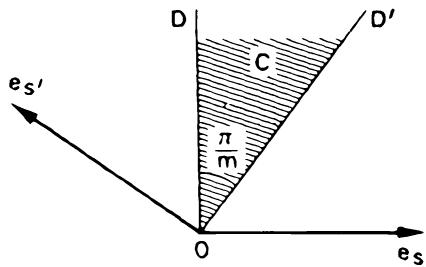
\includegraphics[keepaspectratio]{images/part001_dfbe6528.jpg}}\\
图 2

\subsection{W 在诸室的并中的基本域}

我们沿用第 4 号的记号。对于 \(s \in S\) ，用 \(H_s\) 表示 \(E^*\) 中正交于 \(e_s\) 的超平面，用 \(\overline{A_s}\) 表示由 \(x^* \in E^*\) （满足 \(\langle x^*, e_s \rangle \geqslant 0\) ）构成的集合，并用 \(\overline{C}\) 表示诸 \(\overline{A_s}\) （\(s \in S\) ）的交。对于弱拓扑 \(\sigma(E^*, E)\) （它由 \(E^*\) 与 \(E\) 之间的对偶性定义；《拓扑向量空间》，第 II 章，§6，第 2 号），诸 \(\overline{A_s}\) 是闭半空间，而 \(\overline{C}\) 是一个闭凸锥。此外，\(\overline{C}\) 是 C 的闭包；事实上，若 \(x^* \in \overline{C}\) 且 \(y^* \in C\) ，则 \(x^* + ty^* \in C\) （对每个实数 \(t > 0\) ），且 \(x^* = \lim_{t \to 0} (x^* + ty^*)\) 。

对于 \(X\subset S\) ，置

\[
C _ {X} = \left(\bigcap_ {s \in X} H _ {s}\right) \cap \left(\bigcap_ {s \in S - X} A _ {s}\right).
\]

我们有 \(C_X \subset \overline{C}\) ，\(C_{\varnothing} = C\) 且 \(C_S = \{0\}\) 。诸集合 \(C_X\) （\(X \in B(S)\) ）构成 \(\overline{C}\) 的一个划分。

另一方面，回忆（第 IV 章，§1，第 8 号）\(\mathbf{W}_{\mathbf{X}}\) 表示 \(\mathbf{W}\) 的由 \(\mathbf{X}\) 生成的子群。显然 \(w(x^{*}) = x^{*}\) （对于 \(w \in \mathbf{W}_{\mathbf{X}}\) 与 \(x^{*} \in \mathbf{C}_{\mathbf{X}}\) ）。

命题 5. 设 \(X, X' \subset S\) 且 \(w, w' \in W\) 。若 \(w(C_X) \cap w'(C_{X'}) \neq \emptyset\) ，则 \(X = X'\) ，\(wW_X = w'W_{X'}\) 且 \(w(C_X) = w'(C_{X'})\) 。

我们立即化归到 \(w' = 1\) 的情形。证明对长度 \(n\) （\(w\) 的长度）作归纳。若 \(n = 0\) ，断言是显然的。若 \(l(w) > 0\) ，则存在 \(s \in S\) 使 \(l(sw) = l(w) - 1\) ，于是（参见~第 4 号末尾）\(w(C) \subset s(A_s)\) ，从而 \(w(\overline{C}) \subset s(\overline{A_s})\) 。由于 \(\overline{C} \subset \overline{A_s}\) ，由此得到

\[
\overline {{{\mathrm{C}}}} \cap w (\overline {{{\mathrm{C}}}}) \subset \mathrm{H} _ {s}.
\]

于是 \(s(x^{*}) = x^{*}\) （对所有 \(x^{*} \in \overline{\mathrm{C}} \cap w(\overline{\mathrm{C}})\) ），从而更对所有

\[
x ^ {*} \in \mathrm{C} _ {\mathrm{X} ^ {\prime}} \cap w (\mathrm{C} _ {\mathrm{X}}).
\]

因此，关系 \(C_{X'} \cap w(C_X) \neq \varnothing\) 一方面蕴含 \(C_{X'} \cap H_s \neq \varnothing\) ，从而 \(s \in X'\) ；另一方面蕴含 \(C_{X'} \cap sw(C_X) \neq \varnothing\) 。于是归纳假设表明 \(X = X'\) 且 \(swW_X = W_{X'} = W_X\) ，故 \(sw \in W_X\) ，且 \(w \in W_X\) （由于 \(s \in W_X\) ）。由此得到 \(wW_X = W_{X'}\) 以及 \(w(C_X) = C_X = C_{X'}\) 。

推论. 设 X 是 S 的子集，\(x^{*}\) 是 \(C_{X}\) 的一个元素。\(x^{*}\) 在 W 中的稳定子是 \(W_{X}\) 。

现在设 U 为诸 \(w(\overline{\mathbf{C}})\) （\(w \in W\) ）的并，并设 F 为 U 中形如 \(w(\mathrm{C}_{X})\) 的子集（其中 \(X \subset S\) 且 \(w \in W\) ）所成的集合。由上所述，F 是 U 的一个划分。

命题 6. (i) 锥 U 是凸的。

\begin{enumerate}
\def\labelenumi{(\roman{enumi})}
\setcounter{enumi}{1}
\item
  U 中所含的每个闭线段只与 \(\mathfrak{F}\) 中的有限多个元素相交。
\item
  锥 \(\overline{\mathbf{C}}\) 是 W 在 U 上作用的一个基本域。
\end{enumerate}

为证明 (iii)，只需证明：若 \(x^{*}, y^{*} \in \overline{\mathbb{C}}\) 与 \(w \in \mathbb{W}\) 满足 \(w(x^{*}) = y^{*}\) ，则 \(x^{*} = y^{*}\) 。现在存在两个子集 \(\mathbf{X}\) 与 \(\mathbf{Y}\) （\(\mathbf{S}\) 中的），使得 \(x^{*} \in \mathrm{C}_{\mathbf{X}}\) 且 \(y^{*} \in \mathrm{C}_{\mathbf{Y}}\) ；我们有 \(w(\mathrm{C}_{\mathbf{X}}) \cap \mathrm{C}_{\mathbf{Y}} \neq \emptyset\) ，而命题 5 表明 \(\mathbf{X} = \mathbf{Y}\) 且 \(w \in \mathrm{W}_{\mathbf{X}}\) ，这就蕴含 \(x^{*} = y^{*}\) 。

现在设 \(x^{*}, y^{*} \in \mathrm{U}\) ；我们将证明线段 \([x^{*}y^{*}]\) 被 \(\mathfrak{F}\) 中有限多个元素所覆盖，这就同时建立了 (i) 与 (ii)。把 \(x^{*}\) 与 \(y^{*}\) 用 \(\mathrm{W}\) 的同一个元素来变换，我们可以假设 \(x^{*} \in \overline{\mathrm{C}}\) 。设 \(w \in \mathrm{W}\) 满足 \(y^{*} \in w(\overline{\mathrm{C}})\) 。我们对 \(w\) 的长度作归纳论证。对于 \(s \in \mathrm{S}\) ，关系 \(w(\overline{\mathrm{C}}) \not\subset \overline{\mathrm{A}_{s}}\) 等价于 \(w(\mathrm{C}) \notin \mathrm{A}_{s}\) ，从而等价于 \(l(sw) < l(w)\) （参见~第 4 号）。于是第 IV 章 §1 第 8 号的命题 7 表明，只存在有限多个 \(s \in \mathrm{S}\) 满足 \(w(\overline{\mathrm{C}}) \not\subset \overline{\mathrm{A}_{s}}\) 。于是，集合 \(T\) （由那些 \(s \in S\) 组成，其中 \(\langle y^{*}, e_{s} \rangle < 0\) ）是有限的。另一方面，交 \(\overline{\mathrm{C}} \cap [x^{*}y^{*}]\) 是一个闭线段 \([x^{*}z^{*}]\) 。若 \(z^{*} = y^{*}\) ，即若 \(y^{*} \in \overline{\mathrm{C}}\) ，则存在子集 \(X\) 与 \(Y\) （\(S\) 中的），使得 \(x^{*} \in C_{X}\) 且 \(y^{*} \in C_{Y}\) 。开线段 \(|x^{*}y^{*}|\) 于是含于 \(C_{X \cap Y}\) ，故 \([x^{*}y^{*}] \subset C_{X} \cup C_{Y} \cup C_{X \cap Y}\) 。若 \(z^{*} \neq y^{*}\) ，则存在 \(s \in T\) 使 \(z^{*} \in H_{s}\) 。于是 \(w(C) \not\subset A_{s}\) 且 \(l(sw) < l(w)\) 。从而归纳假设表明，线段 \([z^{*}y^{*}] = s([z^{*}(s(y^{*}))])\) 被 \(\mathfrak{F}\) 的有限多个元素所覆盖，因而

\[
\left[ x ^ {*} y ^ {*} \right] = \left[ x ^ {*} z ^ {*} \right] \cup \left[ z ^ {*} y ^ {*} \right]
\]

因为 \([x^{*}z^{*}]\subset \overline{\mathbf{C}}.\)

\subsection{Coxeter 群的几何表示的不可约性}

我们沿用前面各号的记号，并假设 S 有限。

命题 7. 假设 (W,S) 是不可约的（第 IV 章，§1，第 9 号）。设 \(\mathbf{E}^0\) 是 E 的关于 \(\mathbf{B}_{\mathbf{M}}\) 与 E 正交的子空间。群 W 平凡地作用于 \(\mathbf{E}^0\) ，并且 E 的每个异于 E 且在 W 下稳定的子空间都含于 \(\mathbf{E}^0\) 。

若 \(x \in \mathrm{E}^0\) ，则 \(\sigma_s(x) = x - 2\mathrm{B}_{\mathrm{M}}(e_s, x)e_s = x\) 对所有 \(s \in \mathrm{S}\) 成立。由于 \(\mathrm{W}\) 由 \(\mathrm{S}\) 生成，由此可知 \(\mathrm{W}\) 平凡地作用于 \(\mathrm{E}^0\) 。

设 \(E'\) 是 \(E\) 的一个在 \(W\) 下稳定的子空间。设 \(s, s' \in S\) 是在图 \(\Gamma\) （即 \((W, S)\) 的图；第 IV 章，§1，第 9 号）中相连的两个元素；回忆这意味着 \(m(s, s') \geqslant 3\) 。假设 \(e_s \in E'\) 。则 \(\sigma_{s'}(e_s) \in E'\) ，且由于 \(e_{s'}\) 在 \(\sigma_{s'}(e_s)\) 中的系数非零，我们有 \(e_{s'} \in E'\) 。由于 \(\Gamma\) 连通，由此可知，若 \(E'\) 含有某个 \(e_s\) ，则它含有它们全体并与 \(E\) 重合。除这一情形外，由 §2 第 2 号命题 3 可知，对所有 \(s \in S\) ，\(E'\) 含于超平面 \(H_s\) （正交于 \(e_s\) ）。由于诸 \(H_s\) 的交等于 \(E^0\) ，命题得证。

推论. 假设 (W, S) 是不可约的。则：

\begin{enumerate}
\def\labelenumi{\alph{enumi})}
\item
  若 \(\mathrm{B_M}\) 非退化，则 W-模 E 是绝对单的。
\item
  若 \(\mathrm{B_M}\) 退化，则 W-模 E 不是半单的。
\end{enumerate}

在情形 \(a\) ，命题 7 表明 \(E\) 是单的，从而也是绝对单的（§ 2，第 1 号，命题 1）。

在情形 \(b\) ，有 \(\mathrm{E}^0 \neq 0\) ，\(\mathrm{E} \neq \mathrm{E}^0\) （因为 \(\mathrm{B}_{\mathrm{M}} \neq 0\) ），且命题 7 表明 \(\mathrm{E}^0\) 没有在 W 下稳定的补空间；因此 W-模 E 不是半单的。

\subsection{有限性判别准则}

我们沿用前面各号的记号，并假设 S 有限。

定理 2. 以下性质等价：

\begin{enumerate}
\def\labelenumi{(\arabic{enumi})}
\item
  W 是有限的。
\item
  型 \(B_{M}\) 是正的且非退化的。
\item
  \(\Longrightarrow\) (2). 设 \(S = \bigcup_{i} S_{i}\) 是 \(S\) 分解为连通分支的分解（第 IV 章，§ 1，第 9 号），并设 \(W = \prod_{i} W_{i}\) 是 \(W\) 的相应分解。空间 \(E\) 可与诸空间 \(E_{i} = R^{S_{i}}\) 的直和等同，而 \(B_{M}\) 可与诸相应的型 \(B_{M_{i}}\) 的直和等同。于是我们化归到 \((W, S)\) 不可约的情形。由于假设 \(W\) 有限，\(E\) 是半单的 \(W\) -模（附录，命题 2）。由命题 5 的推论可知 \(E\) 是绝对单的。设 \(B'\) 是 \(E\) 上一个正的非退化型，并设 \(B''\) 是它在 \(W\) 下诸变换的和。由于 \(B''\) 在 \(W\) 下不变，它与 \(B_{M}\) 成比例（ \(\S 2\) ，第 1 号，命题 1）；由于 \(B_{M}(e_{s}, e_{s}) = 1\) （对所有 \(s \in S\) ）成立，比例系数 \(>0\) ，而由于 \(B''\) 是正的，\(B_{M}\) 亦然，这就证明了 (2)。
\item
  \(\Longrightarrow\) (1). 若 \(B_{M}\) 正且非退化，则正交群 \(\mathbf{O}(B_{M})\) 是紧的（《积分》第 VII 章，§3，第 1 号）。由于 \(\sigma(W)\) 是 \(\mathbf{O}(B_{M})\) 的离散子群（定理 1 的推论 3），可知 \(\sigma(W)\) 有限，从而 W 亦有限。证毕。
\end{enumerate}

下面的结果已在证明过程中得到建立：

推论. 若 \((\mathrm{W},\mathrm{S})\) 不可约且有限，则 \(\mathbf{E}\) 是绝对单的 W-模。

定理 2 所提供的有限性判别准则使得可以对所有有限 Coxeter 群进行分类（参见~第 VI 章，§4）。我们在这里只限于下面的初步结果：

命题 8. 若 W 有限，则 (W, S) 的图是一个森林（第 IV 章，附录）。

若不然，这个图将包含一个回路 \((s_{1},\ldots,s_{n})\) ，其中 \(n\geqslant3\) 。置 \(m_{i}=m(s_{1},s_{i+1})\) （\(1\leqslant i<n\) ）及 \(m_{n}=m(s_{n},s_{1})\) ，这就意味着对所有 i 有 \(m_{i}\geqslant3\) 。设

\[
x = e _ {s _ {1}} + \dots + e _ {s _ {n}}.
\]

于是 \(\mathrm{B_M}(x,x) = n + 2\sum_{i < j}\mathrm{B_M}(e_{s_i},e_{s_j})\) 。而

\[
\mathrm{B} _ {\mathrm{M}} (e _ {s _ {i}}, e _ {s _ {i + 1}}) = - \cos \frac {\pi}{m _ {i}} \leqslant - \cos \frac {\pi}{3} \leqslant - \frac {1}{2},
\]

对 \(\mathrm{B}_{\mathbb{M}}(e_{s_n}, e_{s_i})\) 同样如此。由于和中其余各项 \(\leqslant 0\) ，我们得到

\[
\mathrm{B} _ {\mathrm{M}} (x, x) \leqslant n - n = 0,
\]

这与 \(B_{M}\) 正且非退化相矛盾。

推论. 若 (W, S) 不可约且有限，则其图是一棵树。

事实上，连通的森林是树。

与 §3 结果的比较。

首先设 \((W,S)\) 是一个有限 Coxeter 群。用 \((x|y)\) 表示型 \(\mathrm{B}_{\mathbf{M}}(x,y)\) ；由定理 2，这是 E 上的一个标量积。对所有 \(s \in S\) ，设 \(H_{s}\) 是与正交反射 \(\sigma_{s}\) 相伴随的超平面，并设 \(\mathfrak{H}\) 为超平面族 \(w(\mathrm{H}_{s})\) （其中 \(s \in S\) ，\(w \in W\) ）。设 \(C_{0}\) 为由 \(x \in E\) （满足 \((x|e_{s}) > 0\) ，对所有 \(s \in S\) ）所成的集合。最后，借助 \(\sigma\) 把 W 与空间 E 的正交群 \(\mathbf{O}(\mathbf{E})\) 的一个子群等同起来。

命题 9. 按照前面的记号，W 是 O(E) 的由关于 \(\mathfrak{H}\) 中诸超平面的反射所生成的子群。它是一个本质的群（§3，第 7 号），且 C0 是 E 相对于 \(\mathfrak{H}\) 的一个室。

第一个断言是平凡的。另一方面，若 \(x \in E\) 在 W 下不变，则它与所有 \(e_{s}\) 正交，从而为零；这表明 W 是本质的。最后，同构 \(E \to E^{*}\) （由 \(B_{M}\) 定义）把 \(C_{0}\) 变为第 4 号中的集合 C；在那里证明的性质 \((P_{n})\) 表明，对所有 \(w \in W\) 与所有 \(s \in S\) ，\(w(C_0)\) 不与 \(H_s\) 相交。由此可知 \(C_0\) 含于 \(\mathfrak{H}\) 中诸超平面之并的补集 U，而由于 \(C_0\) 在 U 中连通、开且闭，它是 E 相对于 \(\mathfrak{H}\) 的一个室。证毕。

我们可以把 §3 中证明的所有性质应用于 W 与 \(C_{0}\) 。特别地，\(\overline{C_{0}}\) 是 W 在 E 上作用的一个基本域（换句话说，第 6 号中定义的锥 U 等于整个 E）。

反之，设 E 是一个有限维实向量空间，配备标量积 \((x|y)\) ，并设 W 是 E 的一个本质的有限位移群且保持 0 固定；假设 W 由反射生成。设 \(C_{0}\) 是 E 相对于 W 的一个室（参见~§3），并设 S 是相对于 \(C_{0}\) 的墙的正交反射所成的集合。则 (W, S) 是一个有限 Coxeter 系统（§3，第 2 号，定理 1）。此外，若 \(s \in S\) ，用 \(H_{s}\) 表示 \(C_{0}\) 的与 s 相应的墙，并用 \(e_{s}\) 表示正交于 \(H_{s}\) 且关于 \(H_{s}\) 与 \(C_{0}\) 位于同侧的单位向量。若 \((m(s, s'))\) 表示 (W, S) 的 Coxeter 矩阵，则 §3 的命题 3 与 7 表明

\[
(e _ {s} | e _ {s ^ {\prime}}) = - \cos (\pi / m (s, s ^ {\prime}))
\]

并且诸 \(e_{s}\) 构成 E 的一个基。于是 W 在 E 上的自然表示可与第 3 号的表示 \(\sigma\) 等同。

\subsection{\texorpdfstring{\(\mathbf{B}_{\mathrm{M}}\) 为正且退化的情形}{B\_M 为正且退化的情形}}

在本号中，我们假设 S 有限，\((W, S)\) 不可约，且型 \(B_{M}\) 是正的且退化的。

引理 2. 正交补 \(\mathbf{E}^0\) —— 即 \(\mathbf{E}\) 关于 \(\mathbf{B}_{\mathbf{M}}\) 的正交补 —— 是 1 维的；它由一个元素 \(v = \sum_{s\in S}v_s e_s\) （其中 \(v_{s} > 0\) 对所有 \(s\) 成立）生成。

这由 §3 第 5 号的引理 4（应用于以 \(\mathrm{B}_{\mathbb{M}}(e_s, e_{s'})\) 为元素的矩阵）得出。

设 \(v = \sum_{s} v_s e_s\) 是满足引理 2 的条件且使 \(\sum_{s} v_s = 1\) 的向量，并设 A 是 \(E^*\) 中由 \(y^* \in E^*\) （满足 \(\langle v, y^* \rangle = 1\) ）构成的仿射超平面。若 T 表示 \(v\) 在 \(E^*\) 中的正交补，则 A 具有一个仿射空间的自然结构，以 T 为平移空间。此外，型 \(B_M\) 通过过渡到商在 \(E/E^0\) 上定义一个非退化标量积，从而也在其对偶 T 上定义；这给出仿射空间 A 上的一个欧氏结构（《代数》第 IX 章，§6，第 6 号）。

设 G 是 \(\mathbf{GL}(\mathbf{E})\) 的由保持 v 与 \(B_{M}\) 不变的自同构构成的子群；若 \(g \in G\) ，则逆步映射 \({}^{t}g^{-1}\) 保持 A 与 T 稳定，且通过限制到 A 上定义 A 的一个位移 \(i(g)\) （参见~§3）。立即可见这给出从 G 到 A 的位移群的一个同构。此外，A 的点 a 的稳定子 \(G_{a}\) 可与 Hilbert 空间 T 的正交群等同，从而是紧的。另一方面，G 是一个在无穷远处可数的局部紧群，而 A 是一个 Baire 空间：由此（《积分》第 VII 章，附录，引理 2）可知映射 \(\psi : g \mapsto g(a)\) 定义从 \(G/G_a\) 到 A 的一个同胚。于是 G 适当地作用于 A（《一般拓扑》第 III 章，§4，第 2 号，命题 5）。由于 W 是 G 的子群，它可与 A 的一个位移群等同。我们将证明这个群满足 §3 的假设。更确切地说：

命题 10. 赋予离散拓扑的群 W 适当地作用于 A；它由正交反射生成；它是无限的、不可约的且本质的（§3，第 7 号）。交 C ∩ A 是 W 在 A 中的一个室。若 L\_s 表示 A 中由 A 与 E* 的正交于 e\_s 的超平面相交而得的超平面，则诸 L\_s （对于 s ∈ S）是 C ∩ A 的墙。若 ε\_s 是 T 中正交于 L\_s 且与 C ∩ A 位于 L\_s 同侧的单位向量，则 (ε\_s\textbar ε\_t) = -cos(π/m(s,t)) （对于 s,t ∈ S），且 W 的 Coxeter 矩阵（§3，第 4 号）与 M 等同。

由定理 1 的推论 3，W 在 \(\mathbf{GL}(\mathbf{E})\) 中离散，从而在 \(\mathbf{G}\) 中离散，且适当地作用于 A。设 \(s \in S\) 。由于 \(\operatorname{Card} S \geqslant 2\) ，\(\mathbf{E}^*\) 中正交于 \(e_s\) 的超平面不正交于 \(v\) ，它与 A 的交 \(\mathbf{L}_s\) 确是超平面。于是与 \(s\) 相应的位移是保持 \(\mathbf{L}_s\) 的所有点固定的 2 阶位移：它必然是与 \(\mathbf{L}_s\) 相伴随的正交反射。由此可知 W 由正交反射生成。定理 2 现在表明它是无限的，而命题 7 表明它是本质的且不可约的。

由于 C 是一个开单形锥，其墙是方程为 \(\langle x^{*}, e_{s} \rangle = 0\) （对于 \(s \in S\) ）的超平面，交 \(C \cap A\) 是 A 中诸 \(L_{s}\) 之并的补集的一个凸的、从而连通的开且闭子集。此外，\(C \cap A\) 非空，因为若 \(x^{*} \in C\) ，我们有 \(\langle x^{*}, v \rangle = \sum_{s} v_{s} \langle x^{*}, e_{s} \rangle > 0\) 且 \(\langle x^{*}, v \rangle^{-1} x^{*} \in C \cap A\) 。由此可知 \(C \cap A\) 是 A 相对于诸 \(L_{s}\) 的系统的一个室。此外，\(w(C \cap A) \cap L_{s} = \varnothing\) （对所有 \(w \in W\) ；参见~第 4 号，性质 \((\mathrm{P}_{n})\) ）成立，因而 \(C \cap A\) 是 A 相对于由诸 \(L_{s}\) 经 W 的元素变换所得的系统的一个室；由 §3 第 2 号定理 1 的推论可知，\(C \cap A\) 是 A 相对于 W 的一个室。

设 \(a_{s}^{*}\) 是单形 \(C \cap A\) 的不在 \(L_{s}\) 中的顶点。我们有

\[
\left\langle a _ {s} ^ {*}, e _ {t} \right\rangle = 0
\]

对 \(s,t\in \mathrm{S}\) 且 \(s\neq t\) 成立，且

\[
\langle a _ {s} ^ {*}, e _ {s} \rangle = v _ {s} ^ {- 1} \langle a _ {s} ^ {*}, v \rangle = v _ {s} ^ {- 1}.
\]

设 \(\varepsilon_{s}\) 是 T 中由下列关系式定义的向量：

\[
\left(\varepsilon_ {s} \mid a _ {s} ^ {*} - a _ {t} ^ {*}\right) = v _ {s} ^ {- 1} \text {for} t \in S, t \neq s.
\]

向量 \(\varepsilon_{s}\) 正交于 \(L_{s}\) ，且关于超平面 \(L_{s}\) 与 \(C \cap A\) 位于同侧。此外

\[
\left(\varepsilon_ {s} \mid a _ {s} ^ {*} - a _ {t} ^ {*}\right) = \left\langle e _ {s}, a _ {s} ^ {*} - a _ {t} ^ {*} \right\rangle \text {for all} s, t \in S
\]

这表明 \(\varepsilon_{s}\) 是 \(e_{s}\) 的类在从 \(E/E^{0}\) 到 T 的同构（由二次型 \(B_{M}\) 给出）下的像。由此得到

\[
(\varepsilon_ {s} | \varepsilon_ {t}) = \mathrm{B} _ {\mathrm{M}} (e _ {s}, e _ {t}).
\]

因此 \(\varepsilon_{s}\) 是单位向量，而命题 10 的最后一个断言得证。

配备群 W 的欧氏仿射空间 A 称为与 Coxeter 矩阵 M 相伴随的空间，我们记之为 \(A_{M}\) 。

命题 10 有一个逆命题：

命题 11. 设 W 是欧氏仿射空间 A 的一个位移群，满足 §3 的假设。假设 W 是无限的、本质的且不可约的。则与 W 的 Coxeter 矩阵 M 相伴随的型 \(B_{M}\) 是正的且退化的，并且存在唯一的从与 M 相伴随的仿射空间 \(A_{M}\) 到 A 的同构，它与 W 的作用交换。这个同构把 \(A_{M}\) 的标量积变为 A 的标量积的倍数。

设 \(C_0\) 是 A 的一个室，并设 S 是相对于 \(C_0\) 的墙的正交反射所成的集合。若 \(\eta_s\) 表示正交于与反射 s 相伴随的超平面 \(N_s\) 且关于 \(N_s\) 与 \(C_0\) 位于同侧的单位向量（§3，命题 3），则型 \(B_M\) 满足 \(B_M(e_s, e_t) = (\eta_s | \eta_t)\) （对于 \(s, t \in S\) ）。从而它是正的。由于诸 \(\eta_s\) 线性相关（§3，第 9 号，命题 8），它是退化的。

于是我们可以把前面的构造应用于 M。沿用与上面相同的记号，\((\varepsilon_{s}|\varepsilon_{t}) = (\eta_{s}|\eta_{t})\) ，且存在唯一的 Hilbert 空间同构 \(\varphi\) ，从 T 到 A 的平移空间，使得 \(\varphi(\varepsilon_{s}) = \eta_{s}\) 。设 a 与 b 是 \(C_{0}\) 的两个不同顶点，\(s_{0}\) 是 S 中使 \(a \notin N_{s_{0}}\) 的反射。置 \(\lambda = (\eta_{s}|a - b)\) ，并设 \(\psi\) 是由下式定义的从 \(A_{M}\) 到 A 的仿射双射

\[
\psi \left(a _ {s _ {0}} + x\right) = a + v _ {s _ {0}} \lambda \varphi (x) \text {for} x \in \mathrm{T}.
\]

于是立即可见 \(\psi(\mathrm{L}_{s}) = \mathrm{N}_{s}\) （对所有 \(s \in S\) ），且 \(\psi\) 把 \(A_{M}\) 的标量积变为 A 上标量积的倍数。立即得到 \(\psi\) 与 W 的作用交换。最后，\(\psi\) 的唯一性是明显的，因为例如 \(a_{s}\) 是 \(A_{M}\) 中在诸反射 \(t \in S, t \neq s\) 下不变的唯一点。

\section{对称代数中的不变量}

\subsection{分次代数的 Poincaré 级数}

设 K 是一个有单位元且不退化为 0 的交换环。设 M 是一个 Z 型分次 K-模，\(M_{n}\) 是 M 中次数为 n 的齐次元素所成的集合。假设每个 \(M_{n}\) 都是自由的且有限型的。于是秩 \(\operatorname{rk}_{\mathbf{K}}(\mathbf{M}_{n})\) 对所有 n 有定义（《交换代数》第 II 章，§5，第 3 号）。

定义 1. 若存在 \(n_0 \in \mathbf{Z}\) 使 \(M_n = 0\) （对于 \(n \leqslant n_0\) ），则形式级数 \(\sum_{n \geqslant n_0} \mathrm{rk}_K(M_n) T^n\) （\(\mathbf{Q}((T))\) 的一个元素）称为 \(M\) 的 Poincaré 级数，记为 \(P_M(T)\) 。

设 \(M'\) 是另一个 Z 型分次 K-模，\((M_n')_{n \in \mathbf{Z}}\) 是它的分次。假设 \(M_n'\) 对小于某个数的 n 为零。则

\[
\mathrm{P} _ {\mathrm{M} \oplus \mathrm{M} ^ {\prime}} (\mathrm{T}) = \mathrm{P} _ {\mathrm{M}} (\mathrm{T}) + \mathrm{P} _ {\mathrm{M} ^ {\prime}} (\mathrm{T})\tag{1}
\]

而若给 \(\mathbf{M} \otimes_{\mathbf{K}} \mathbf{M}'\) 赋予总分次（《代数》第 II 章，§11，第 5 号），则

\[
\mathrm{P} _ {\mathrm{M} \otimes \mathrm{M} ^ {\prime}} (\mathrm{T}) = \mathrm{P} _ {\mathrm{M}} (\mathrm{T}) \mathrm{P} _ {\mathrm{M} ^ {\prime}} (\mathrm{T}).\tag{2}
\]

命题 1. 设 \(S = \bigoplus_{n \geqslant 0} S_n\) 是一个交换分次 K-代数，具有一个由齐次且代数无关的元素组成的生成元组 \((x_1, x_2, \ldots, x_m)\) 。设 \(d_i\) 是 \(x_i\) 的次数，并假设 \(d_i > 0\) （对所有 \(i\) ）。则诸 \(S_n\) 在 \(K\) 上是自由的且有限秩的，并且

\[
\mathrm{P} _ {\mathrm{S}} (\mathrm{T}) = \prod_ {i = 1} ^ {m} (1 - \mathrm{T} ^ {d _ {i}}) ^ {- 1}.\tag{3}
\]

事实上，S 可与张量积 \(K[x_{1}] \otimes \cdots \otimes K[x_{m}]\) 等同，后者赋予总分次。\(K[x_{i}]\) 的 Poincaré 级数是

\[
\sum_ {n \geqslant 0} \mathrm{T} ^ {n d _ {i}} = (1 - \mathrm{T} ^ {d _ {i}}) ^ {- 1},
\]

于是只需应用 (2)。

在命题 1 的假设下，我们将称 S 是 K 上的一个分次多项式代数。

推论. 诸次数 \(d_{i}\) 由 S 确定，至多相差次序。

事实上，\(\mathrm{P}_{\mathrm{S}}(\mathrm{T})\) 的逆是多项式 \(\mathrm{N}(\mathrm{T}) = \prod_{i=1}(1 - \mathrm{T}^{d_i})\) ，从而是唯一确定的。若 q 是一个整数 \(\geqslant 1\) 且 \(\zeta \in C\) 是一个本原 q 次单位根，则根 \(\zeta\) 在 \(\mathrm{N}(\mathrm{T})\) 中的重数等于 \(d_{i}\) 中是 q 的倍数的个数。当 q 充分大时这个数为零。于是等于 q 的 \(d_{i}\) 的个数由递降归纳唯一确定。

诸整数 \(d_{i}\) 称为 S 的特征次数。当 K 是域时，它们的个数等于 S 在 K 上的超越次数；在一般情形我们也把它称为 S 在 K 上的超越次数。它是多项式 N(T) 的根 1 的重数。

设 \(S = \bigoplus_{n \geqslant 0} S_n\) 是一个交换分次 K-代数，\(R = \bigoplus_{n \geqslant 0} R_n\) 是 S 的一个分次子代数。假设每个 \(R_n\) 都是自由的且有限型的，且 R-模 S 具有一个由齐次元素 \(z_1, z_2, \ldots, z_N\) （次数分别为 \(f_1, f_2, \ldots, f_N\) ）组成的有限基。于是，若用 M 表示分次 K-模 \(\sum_{j=1}^{N} Kz_j\) ，则分次 K-模 S 同构于 \(R \otimes_K M\) ，从而每个 \(S_n\) 都是自由的且有限型的，并且

\[
P _ {S} (T) = P _ {M} (T) P _ {R} (T) = \left(\sum_ {j = 1} ^ {N} T ^ {f _ {j}}\right) P _ {R} (T).\tag{4}
\]

命题 2. 沿用前面的记号，并假设 \(S\) 与 \(R\) 是分次多项式代数。

\begin{enumerate}
\def\labelenumi{(\roman{enumi})}
\item
  R 与 S 有相同的超越次数 \(r\) （在 \(K\) 上）。
\item
  设 \(p_1, \ldots, p_r\) （分别为 \(q_1, \ldots, q_r\) ）是 \(S\) （分别为 \(R\) ）的特征次数。则
\end{enumerate}

\[
\prod_ {i = 1} ^ {r} \left(1 - \mathrm{T} ^ {q _ {i}}\right) = \left(\sum_ {j = 1} ^ {\mathrm{N}} \mathrm{T} ^ {f _ {j}}\right) \prod_ {i = 1} ^ {r} \left(1 - \mathrm{T} ^ {p _ {i}}\right).
\]

\begin{enumerate}
\def\labelenumi{(\roman{enumi})}
\setcounter{enumi}{2}
\tightlist
\item
  \(Np_{1}p_{2}\ldots p_{r}=q_{1}q_{2}\ldots q_{r}.\)
\end{enumerate}

公式 (4) 首先表明根 1 的重数在多项式 \(\mathrm{P}_{\mathrm{S}}(\mathrm{T})^{-1}\) 与 \(\mathrm{P}_{\mathrm{R}}(\mathrm{T})^{-1}\) 中相同，再考虑到 (3)，就同时证明了 (i) 与 (ii)。

由 (ii) 得到

\[
\prod_ {i = 1} ^ {r} \left(1 + \mathrm{T} + \mathrm{T} ^ {2} + \dots + \mathrm{T} ^ {q _ {i} - 1}\right) = \left(\sum_ {j = 1} ^ {\mathrm{N}} \mathrm{T} ^ {f _ {j}}\right) \prod_ {i = 1} ^ {r} \left(1 + \mathrm{T} + \mathrm{T} ^ {2} + \dots + \mathrm{T} ^ {p _ {i} - 1}\right).
\]

在此关系中置 \(\mathrm{T} = 1\) 即得 (iii)。

注. 设 \(S = K[X_1, \ldots, X_n]\) 是 \(K\) 上的一个分次多项式代数，\(d_i\) 是 \(X_i\) 的次数，\(F(X_1, \ldots, X_n)\) 是一个次数为 \(m\) 的 \(S\) 的齐次元素。则

\[
\sum_ {i = 1} ^ {n} d _ {i} X _ {i} \frac {\partial F}{\partial X _ {i}} = m F.\tag{5}
\]

事实上，立即可见把每个次数为 p 的齐次元素 z 变为 pz 的、从 S 到 S 的 K-线性映射 D 是 S 的一个求导。于是

\[
m \mathrm{F} (\mathrm{X} _ {1}, \dots , \mathrm{X} _ {n}) = \mathrm{D} (\mathrm{F} (\mathrm{X} _ {1}, \dots , \mathrm{X} _ {n})) = \sum_ {i = 1} ^ {n} \mathrm{D} (\mathrm{X} _ {i}) \frac {\partial \mathrm{F}}{\partial \mathrm{X} _ {i}} = \sum_ {i = 1} ^ {n} d _ {i} \mathrm{X} _ {i} \frac {\partial \mathrm{F}}{\partial \mathrm{X} _ {i}}.
\]

\subsection{有限线性群的不变量：模性质}

设 K 是一个交换环，V 是一个 K-模，G 是一个作用于 V 的群。我们知道 V 的每个自同构唯一地开拓为对称代数 \(S = \mathbf{S}(V)\) 的自同构，从而 G 作用于这个代数。若 \(x \in S\) 且 \(g \in G\) ，用 \(g_{S}.x\) 表示 x 在 g 下的像。设 R 是 S 中由在 G 下不变的元素构成的子代数 \(S^{G}\) 。

假设 G 有限，V 有限型，且 K 是 noether 的。于是 S 是一个有限型 R-模，而 R 是一个有限型 K-代数（《交换代数》第 V 章，§1，第 9 号，定理 2）。假设 S 是整的，并设 N 是它的分式域。R 的分式域 L 是 N 中在 G 下不变的元素所成的集合（出处同前，命题 23 的推论），故 N 是 L 的一个 Galois 扩张。N 的每个元素都可写成 z/t，其中 \(z \in S\) 且 \(t \in R\) （出处同前，命题 23）。由《代数》第 II 章 §7 第 10 号命题 26 的推论 3，R-模 S 的秩是 {[}N : L{]}。假设 G 忠实地作用于 V。于是 N 在 L 上的 Galois 群可与 G 等同，故 {[}N : L{]} = Card G；从而

\[
\operatorname{rk} _ {\mathsf {R}} (\mathrm{S}) = [ \mathrm{N}: \mathrm{L} ] = \operatorname{Card} (\mathrm{G}).\tag{6}
\]

对任意分次代数 \(A = A_{0} \oplus A_{1} \oplus \cdots \oplus A_{n} \oplus \cdots\) ，用 \(A_{+}\) 表示理想 \(\bigoplus_{n > 0} A_{n}\) 。

定理 1. 设 K 是一个交换域，V 是 K 上一个有限维向量空间，S = S(V) 是 V 的对称代数，G 是 V 的一个有限自同构群，R 是 S 中由在 G 下不变的元素组成的分次子代数。假设 G 由伪反射生成（§2，第 1 号），且 q = Card(G) 与 K 的特征互素。则 R-模 S 具有一个由 q 个齐次元素组成的基。

\begin{enumerate}
\def\labelenumi{\alph{enumi})}
\item
  由于 \(S/(R_{+}S)\) 的每个子模在 \(R_0 = K\) 上都是自由的，只需（《代数》第 II 章，§11，第 4 号，命题 7）证明从 \(R_{+} \otimes_{R} S\) 到 \(S\) 的典范同态是单射。对任意 R-模 \(E\) ，用 \(T(E)\) 表示 R-模 \(\text{Ker}(R_{+} \otimes_{R} E \to E)\) （*换句话说，\(T(E) = \text{Tor}_{1}^{R}(R/R_{+}, E)_*\) ）。若 \(E, E'\) 是两个 R-模而 \(u\) 是从 \(E\) 到 \(E'\) 的同态，则同态 \(1 \otimes u\) （从 \(R_{+} \otimes E\) 到 \(R_{+} \otimes E'\) ）通过限制到 \(T(E)\) 上定义一个从 \(T(E)\) 到 \(T(E')\) 的同态，我们记之为 \(T(u)\) 。若 \(u'\) 是从 \(E'\) 到某个 R-模 \(E''\) 的同态，则有 \(T(u' \circ u) = T(u') \circ T(u)\) 。于是，若 G R-线性地作用于 \(E\) ，则 G 作用于 \(T(E)\) 。
\item
  群 G R-线性地作用于 S，从而也作用于 T(S)。此外，T(S) 具有一个分次 S-模的自然结构。我们首先证明，若 \(g \in G\) ，则 g 把 T(S) 的每个元素 x 变为模 \(S_{1}T(S)\) 与 x 同余的元素。只需对 g 是伪反射的情形证明这一点。此时存在 V 中一个非零向量 v，使得 \(g(x) - x \in Kv\) （对所有 \(x \in V\) ）。由于 V 生成 S，由此可知 \(g_{S}\) 平凡地作用于 S/Sv。于是，对任意 \(y \in S\) ，存在 S 中一个元素 \(h(y)\) 使得
\end{enumerate}

\[
g _ {\mathrm{S}} (y) - y = h (y) v.
\]

由于 S 是整的且 v 非零，这个元素由 y 唯一确定；立即可见 h 是 R-模 S 的一个次数为 -1 的自同态。于是 \(g_{S} - 1_{S} = m_{v} \circ h\) ，其中 \(m_{v}\) 表示 S 中比率为 v 的位似。由此，

\[
\mathrm{T} (g _ {\mathrm{S}}) - 1 _ {\mathrm{T(S)}} = \mathrm{T} (g _ {\mathrm{S}} - 1 _ {\mathrm{S}}) = \mathrm{T} (m _ {v}) \circ \mathrm{T} (h),
\]

其像含于 \(vT(S)\) ，这就证明了我们的断言。

\begin{enumerate}
\def\labelenumi{\alph{enumi})}
\setcounter{enumi}{2}
\tightlist
\item
  我们证明 \(T(S)\) 中在 G 下不变的任何元素为零。事实上，设 Q 是 R-模 S 的由下式定义的自同态
\end{enumerate}

\[
\mathrm{Q} (y) = q ^ {- 1} \sum_ {g \in G} g _ {\mathrm{S}} (y)
\]

（对所有 \(y \in S\) ）。则 \(Q(S) = R\) 。于是我们可以写 \(Q = i \circ Q'\) ，其中 \(Q'\) 是从 R-模 S 到 R-模 R 的同态，而 i 表示 R 到 S 中的典范单射。从而 \(T(Q) = T(i) \circ T(Q')\) ，且 \(T(Q') = 0\) ，因为 \(T(R) = \text{Ker}(R_{+} \otimes R \to R) = 0\) 。于是

\[
0 = \mathrm{T} (\mathrm{Q}) = q ^ {- 1} \sum_ {g \in \mathrm{G}} \mathrm{T} (g _ {\mathrm{S}}).
\]

而 \(q^{-1} \sum_{g \in G} T(g_S)\) 保持 \(T(S)\) 中在 G 下不变的元素不动。因此这些元素为零。

\begin{enumerate}
\def\labelenumi{\alph{enumi})}
\setcounter{enumi}{3}
\tightlist
\item
  假设 \(T(S) \neq 0\) 。在 \(T(S)\) 中存在一个次数最小的非零齐次元素 \(u \neq 0\) 。由 b)，u 在 G 下不变。由 c)，u = 0。这是矛盾，故 \(T(S) = 0\) 。证毕。
\end{enumerate}

注. 1) 由《代数》第 II 章 §11 第 4 号命题 7 可知，若 \((z_{1},\ldots ,z_{q})\) 是 S 的一个齐次元素族，其典范像在 \(\mathrm{S / (R_+S)}\) 中构成 \(\mathrm{S / (R_+S)}\) 在 K 上的基，则 \((z_{1},\ldots ,z_{q})\) 是 S 在 R 上的基。

\begin{enumerate}
\def\labelenumi{\arabic{enumi})}
\setcounter{enumi}{1}
\tightlist
\item
  设 \(g\) 是 \(V\) 的一个伪反射，其阶 \(n \geqslant 2\) 有限且与 \(K\) 的特征互素。由 Maschke 定理（附录，命题 2），\(V\) 可分解为 \(D \oplus H\) ，其中 \(H\) 是由 \(V\) 中在 \(g\) 下不变的元素组成的超平面，而 \(D\) 是一条直线，\(g\) 在其上通过乘以一个本原 \(n\) 次单位根作用。当 \(K = R\) 时，这仅当 \(n = 2\) 时才可能，此时 \(g\) 是一个反射；在这种情形，定理 1 所适用的群是有限 Coxeter 群。（相反，对 K = C，定理 1 适用于某些不是 Coxeter 群的群。）\(^{3}\)
\end{enumerate}

定理 2. 沿用定理 1 的假设与记号。

\begin{enumerate}
\def\labelenumi{(\roman{enumi})}
\item
  存在 \(S\) 的一个分次向量子空间，它构成 \(R_{+}S\) 在 \(S\) 中的补，且在 \(G\) 下稳定。
\item
  设 U 是这样一个补。从 \(U \otimes_{K} R\) 到 S 的典范同态是 G-模的同构，且 G 在 U（分别为 S）中的表示同构于 G 在 K（分别为 R）上的正则表示。
\end{enumerate}

事实上，对任意整数 \(n \geqslant 0\) ，K-向量空间 \(S_n\) 与 \((R_+S) \cap S_n\) 在 \(G\) 下稳定，且由 Maschke 定理（附录，命题 2）可知存在一个 G-稳定的子空间 \(U_n\) ，它构成 \((R_+S) \cap S_n\) 在 \(S_n\) 中的补。于是 \(\sum_{n \geqslant 0} U_n\) 是 \(R_+S\) 在 \(S\) 中的一个 G-稳定的补，由此得 (i)。

设 U 是 S 的一个分次向量子空间，它在 S 中构成 \(R_{+}S\) 的补且在 G 下稳定。由注 1，K-向量空间 U 的每个基也是 R-模 S 的基，从而是 S 的分式域 N 在 R 的分式域 L 上的基。于是 L-向量空间 N 可与 \(U \otimes_{K} L\) 等同。由于 U 在 G 下稳定，这一等同与 G 的作用相容。G 在 L 上的群代数 \(L[G]\) 可与代数 \(K[G] \otimes_{K} L\) 等同。L 的 Galois 扩张 N 具有正规基（《代数》第 V 章，§10，第 9 号，定理 6），这可以解释为：N（视为 \(L[G]\) -模）同构于 G 在 L 上的正则表示的模。由于 U 在 K 上有限维，由附录命题 1 可知 \(K[G]\) -模 U 同构于 G 在 K 上的正则表示。我们的断言由此立得。

\subsection{有限线性群的不变量：环论性质}

定理 3. 我们沿用定理 1 的假设与记号。在 \(R_{+}\) （R 的理想）的由齐次元素组成的生成元组的集合中，取一个极小元 \((\alpha_{1},\ldots,\alpha_{l})\) 。设 \(k_{i}\) 是 \(\alpha_{i}\) 的次数。假设诸 \(k_{i}\) 与 K 的特征指数互素。则 \(l=\dim V\) ，诸 \(\alpha_{i}\) 生成 K-代数 R，且在 K 上代数无关。特别地，R 是 K 上超越次数为 l 的一个分次多项式 K-代数。

关于 \(k_{i}\) 所作的假设是多余的，但对有限 Coxeter 群的应用而言无关紧要，因为那时 K = R。参见第 5 号，我们将在那里给出定理 3 的另一个证明。

定理 3 由命题 2 (i)、定理 1 以及下面的引理得出：

引理 1. 设 K 是一个交换域，S 是一个分次多项式 K-代数，R 是 S 的一个有限型分次子代数，使得 R-模 S 具有一个由齐次元素组成的基 \((z_{\lambda})_{\lambda \in \Lambda}\) 。在 \(R_{+}\) （R 的理想）的由齐次元素组成的生成元组的集合中，取一个极小元 \((\alpha_{1}, \ldots, \alpha_{s})\) 。假设对所有 i，次数 \(k_{i}\) （\(\alpha_{i}\) 的）与 K 的特征指数 p 互素。则诸 \(\alpha_{i}\) 生成 K-代数 R 且在 K 上代数无关。

由《代数》第 II 章 § 11 第 4 号命题 7，关于 \(\alpha_{i}\) 所作的假设等价于说它们是齐次的，且它们的像在 K-向量空间 \(R_{+}/(R_{+})^{2}\) 中构成该空间的基。这一条件在基域扩张下不变；于是我们可以化归到基域为完满的情形。

族 \((\alpha_{1},\ldots,\alpha_{s})\) 生成代数 R（《交换代数》第 III 章，§1，第 2 号，命题 1）。我们用反证法，假设这个族在 K 上不是代数无关的。

\begin{enumerate}
\def\labelenumi{\arabic{enumi})}
\tightlist
\item
  我们首先证明存在诸族
\end{enumerate}

\[
\left(\beta_ {i}\right) _ {1 \leqslant i \leqslant s}, \quad \left(y _ {k}\right) _ {1 \leqslant k \leqslant r}, \quad \left(d _ {i k}\right) _ {1 \leqslant i \leqslant s, 1 \leqslant k \leqslant r}
\]

它们由 S 的齐次元素组成，且满足下列性质：

\[
\beta_ {i} \in R \text {for all} i, \text {and the} \beta_ {i} \text {are not all zero};\tag{7}
\]

\[
\deg y _ {k} > 0 \text {   for   all   } k;\tag{8}
\]

\[
\alpha_ {i} = \sum_ {k = 1} ^ {r} d _ {i k} y _ {k} \quad \text { for   all } i;\tag{9}
\]

\[
\sum_ {i = 1} ^ {s} \beta_ {i} d _ {i k} = 0 \quad \text { for   all } k.\tag{10}
\]

设 \(X_{1},\ldots,X_{s}\) 是未定元，并给 \(K[X_{1},\ldots,X_{s}]\) 赋予使 \(X_{i}\) 的次数为 \(k_{i}\) 的分次代数结构。存在非零齐次元素 \(H(X_{1},\ldots,X_{s})\) ，它属于 \(K[X_{1},\ldots,X_{s}]\) ，使得 \(H(\alpha_{1},\ldots,\alpha_{s})=0\) ；取 H 为次数最小的。若 \(\partial H/\partial X_{i}\neq0\) ，则多项式 \(\frac{\partial H}{\partial X_{i}}(\alpha_{1},\ldots,\alpha_{s})\) 是 R 的一个非零齐次元素；若 \(p\neq1\) ，则 H 不具有 \(H_{1}^{p}\) （其中 \(H_{1}\in K[X_{1},\ldots,X_{s}]\) ）的形式。取

\[
\beta_ {i} = k _ {i} \frac {\partial \mathrm{H}}{\partial \mathrm{X} _ {i}} (\alpha_ {1}, \dots , \alpha_ {s}).
\]

由于 K 是完满的，多项式 \(\partial H/\partial X_{i} \in K[X_{1},\ldots,X_{s}]\) 不全为零（《代数》第 V 章，§1，第 3 号，命题 4）；鉴于关于 \(k_{i}\) 的假设，诸 \(\beta_{i}\) 亦不全为零。

另一方面，S 可与一个分次多项式代数 \(K[x_{1},\ldots,x_{r}]\) 等同，其中 \(x_{1},\ldots,x_{r}\) 是适当的未定元，次数为适当的 \(m_{i}>0\) 。设 \(D_{k}\) 是 S 上关于 \(x_{k}\) 的偏导数。取 \(d_{ik} = k_i^{-1}\mathrm{D}_k(\alpha_i)\) 。则等式 (10) 成立，因为其左边是 \(\mathrm{D}_k(\mathrm{H}(\alpha_1,\dots ,\alpha_s))\) 。另一方面，若置 \(y_{1} = m_{1}x_{1},\ldots ,y_{r} = m_{r}x_{r}\) ，则等式 (9) 由第 1 号的等式 (5) 得出。

\begin{enumerate}
\def\labelenumi{\arabic{enumi})}
\setcounter{enumi}{1}
\tightlist
\item
  设 \(\mathfrak{b}\) 是 \(R\) 的由诸 \(\beta_{i}\) 生成的理想；存在下述集合的一个子集 \(J\) ：
\end{enumerate}

\[
\mathrm{I} = \{1, 2, \dots , s \}
\]

使得 \((\beta_{i})_{i\in\mathbb{J}}\) 是 b 的一个极小生成元组。则 \(J\neq\varnothing\) ，因为 \(b\neq0\) 。我们将由 (9) 与 (10) 推出：若 \(i\in J\) ，则 \(\alpha_{i}\) 是诸 \(\alpha_{j}\) （\(j\neq i\) ）的 R-线性组合，这与 \((\alpha_{1},\ldots,\alpha_{s})\) 的极小性矛盾，从而完成证明。

存在 R 的齐次元素 \(\gamma_{ji}\) ( \(i \in \mathrm{J}, j \in \mathrm{I} - \mathrm{J}\) ) 使得

\[
\beta_ {j} = \sum_ {i \in J} \gamma_ {j i} \beta_ {i} (j \in I - J).\tag{11}
\]

考虑到 (11)，公式 (10) 给出

\[
\sum_ {i \in \mathrm{J}} \beta_ {i} \left(d _ {i k} + \sum_ {j \in \mathrm{I} - \mathrm{J}} \gamma_ {j i} d _ {j k}\right) = 0.\tag{12}
\]

置

\[
u _ {i k} = d _ {i k} + \sum_ {j \in I - J} \gamma_ {j i} d _ {j k}.\tag{13}
\]

于是

\[
\sum_ {i \in J} \beta_ {i} u _ {i k} = 0.\tag{14}
\]

写 \(u_{ik} = \sum_{\lambda \in \Lambda} \delta_{ik\lambda} z_\lambda\) ，其中诸 \(\delta_{ik\lambda}\) 属于 R。关系式 (14) 蕴含 \(\sum_{i \in J} \beta_i \delta_{ik\lambda} = 0\) （对所有 \(k\) 与 \(\lambda\) ）。若某个 \(\delta_{ik\lambda}\) 有一个次数为 0 的非零齐次分量，则前面的等式将蕴含某个 \(\beta_i\) ( \(i \in J\) ) 是其余元素的 R-线性组合，与 \((\beta_i)_{i \in J}\) 的极小性矛盾。于是 \(\delta_{ik\lambda} \in R_+\) ，从而 \(u_{ik} \in R_+ S\) （对所有 \(i\) 与 \(k\) ）。于是存在 \(u_{ikh} \in S\) 使得 \(u_{ik} = \sum_{h=1}^{s} u_{ikh} \alpha_h\) ，换句话说，由 (13)，

\[
d _ {i k} + \sum_ {j \in I - J} \gamma_ {j i} d _ {j k} = \sum_ {h = 1} ^ {s} u _ {i k h} \alpha_ {h}.\tag{$(15)_{ik}$}
\]

把 \((15)_{ik}\) 的两边乘以 \(y_{k}\) ，并对固定的 i ∈ J 与 \(k = 1, 2, \ldots, r\) 相加；鉴于 (9)，我们得到

\[
\alpha_ {i} + \sum_ {j \in I - J} \gamma_ {j i} \alpha_ {j} = \sum_ {h = 1} ^ {s} \sum_ {k = 1} ^ {r} u _ {i k h} y _ {k} \alpha_ {h}.
\]

取两边的次数为 \(k_i\) 的齐次分量。由于 \(\deg y_k > 0\) ，\(\alpha_i\) 是诸 \(\alpha_j\) （\(j \neq i\) ）的 S-线性组合。由于 S 在 R 上自由且 \(\alpha_1, \ldots, \alpha_s \in \mathrm{R}\) ，由此可知 \(\alpha_i\) 是诸 \(\alpha_j\) （\(j \neq i\) ）的 R-线性组合（《交换代数》第 I 章，§3，第 5 号，命题 9 d))。

推论. 在定理 3 的假设与记号下，R 的特征次数之积是 Card(G)。

事实上，\(\operatorname{rk}_{\mathrm{R}}(S) = \operatorname{Card}(G)\) （公式 (6)，第 2 号）。S 的特征次数都等于 1。于是推论由第 1 号命题 2 (iii) 得出。

引理 2. 设 K 是一个交换域，V 是 K 上一个有限维向量空间，\(S = \bigoplus_{n \geqslant 0} S_n\) 是 V 的对称代数，s 是 V 的一个自同态，\(s^{(n)}\) 是 s 到 \(S_n\) 的典范开拓。则当 T 表示一个未定元时，我们在 K{[}{[}T{]}{]} 中有

\[
\sum_ {n = 0} ^ {\infty} \operatorname{Tr} (s ^ {(n)}) \mathrm{T} ^ {n} = (\det (1 - s \mathrm{T})) ^ {- 1}.
\]

必要时扩张基域，我们可以假设 K 是代数闭的。设 \((e_{1},\ldots,e_{r})\) 是 V 的一个基，s 关于它的矩阵是下三角的，并设 \(\lambda_{1},\ldots,\lambda_{r}\) 是这个矩阵的对角元素。关于按字典序排列的基 \((e_{1}^{i(1)}\ldots e_{r}^{i(r)})_{i(1)+\cdots+i(r)=n}\) （\(S_{n}\) 的），\(s^{(n)}\) 的矩阵是下三角的，其对角元素是诸乘积 \(\lambda_{1}^{i(1)}\ldots\lambda_{r}^{i(r)}\) 。于是

\[
\operatorname{Tr} \left(s ^ {(n)}\right) = \sum_ {i (1) + \dots + i (r) = n} \lambda_ {1} ^ {i (1)} \dots \lambda_ {r} ^ {i (r)},
\]

从而

\[
\begin{array}{l} \sum_ {n = 0} ^ {\infty} \operatorname{Tr} (s ^ {(n)}) \mathrm{T} ^ {n} = \left(\sum_ {n = 0} ^ {\infty} \lambda_ {1} ^ {n} \mathrm{T} ^ {n}\right) \left(\sum_ {n = 0} ^ {\infty} \lambda_ {2} ^ {n} \mathrm{T} ^ {n}\right) \ldots \left(\sum_ {n = 0} ^ {\infty} \lambda_ {r} ^ {n} \mathrm{T} ^ {n}\right) \\ \qquad = (1 - \lambda_ {1} \mathrm{T}) ^ {- 1} (1 - \lambda_ {2} \mathrm{T}) ^ {- 1} \ldots (1 - \lambda_ {r} \mathrm{T}) ^ {- 1} \\ \qquad = (\det (1 - s \mathrm{T})) ^ {- 1}. \end{array}
\]

引理 3. 设 K、V 与 S 如引理 2 中所述，G 是 V 的一个有限自同构群，q 是 G 的阶，R 是 S 中由在 G 下不变的元素组成的分次子代数。假设 K 的特征为 0。则 R 的 Poincaré 级数是

\[
q ^ {- 1} \sum_ {g \in G} (\det (1 - g T)) ^ {- 1}.
\]

事实上，自同态 \(f = q^{-1} \sum_{g \in G} g^{(n)}\) 是 \(S_n\) 到 \(R_n\) 上的一个投影，故 \(\operatorname{Tr}(f) = \dim_K S_n^G\) 。于是 \(R\) 的 Poincaré 级数是

\[
q ^ {- 1} \sum_ {g \in G} \left(\sum_ {n = 0} ^ {\infty} (\operatorname{Tr} g ^ {(n)}) T ^ {n}\right),
\]

于是只需应用引理 2。

命题 3. 在定理 3 的假设与记号下，设 H 是属于 G 且异于 1 的伪反射所成的集合。假设 K 的特征为 0。则 \(\operatorname{Card}(\mathrm{H}) = \sum_{i=1}^{l}(k_i - 1)\) 。

由附录命题 3，我们可以假设 K 是代数闭的。对任意 \(g \in G\) ，设 \(\lambda_{1}(g), \ldots, \lambda_{l}(g)\) 是它的特征值。由于每个 \(g \in G\) 都可对角化（附录，命题 2），g = 1 当且仅当所有 \(\lambda_{i}(g)\) 都等于 1，而 \(g \in H\) 当且仅当等于 1 的 \(\lambda_{i}(g)\) 的个数是 l - 1（此时我们用 \(\lambda(g)\) 表示异于 1 的特征值）。第 1 号的命题 1 与引理 3 证明

\[
q \prod_ {i = 1} ^ {l} (1 - T ^ {k _ {i}}) ^ {- 1} = \sum_ {g \in G} (\det (1 - g T)) ^ {- 1}\tag{16}
\]

在 \(\mathbf{K}[[\mathbf{T}]]\) 中成立，从而在 \(\mathbf{K}(\mathbf{T})\) 中成立。于是，我们在 \(\mathbf{K}(\mathbf{T})\) 中有

\[
q \frac {(1 - T) ^ {l - 1}}{\prod_ {i = 1} ^ {l} (1 - T ^ {k _ {i}})} = \frac {1}{1 - T} + \sum_ {g \in H} \frac {1}{1 - \lambda (g) T} + \sum_ {g \neq 1, g \notin H} \frac {(1 - T) ^ {l - 1}}{\det (1 - g T)},
\]

它可以写成

\[
\begin{array}{c} \frac {q - \prod_ {i = 1} ^ {l} (1 + T + \cdots + T ^ {k _ {i} - 1})}{(1 - T) \prod_ {i = 1} ^ {l} (1 + T + \cdots + T ^ {k _ {i} - 1})} \\ = \sum_ {g \in H} \frac {1}{1 - \lambda (g) T} + \sum_ {g \neq 1, g \notin H} \frac {(1 - T) ^ {l - 1}}{\det (1 - g T)}. \end{array}\tag{17}
\]

由此可知 \(q - \prod_{i=1}^{l} (1 + T + \cdots + T^{k_i - 1})\) 在 T = 1 处为零，故 \(q = k_1 k_2 \ldots k_l\) ，这一点我们已由定理 3 的推论得知。鉴此，设 \(Q(T)\) 是多项式 \((1 - T)^{-1}(q - \prod_{i=1}^{l} (1 + T + \cdots + T^{k_i - 1}))\) 。对等式 \((1 - T)Q(T) = q - \prod_{i=1}^{l} (1 + T + \cdots + T^{k_i - 1})\) 求导并置 T = 1，我们看到 \(-Q(1)\) 是下式在 T = 1 处的值

\[
\begin{array}{l} - \frac {d}{d t} \left(\prod_ {i = 1} ^ {l} (1 + T + \dots + T ^ {k _ {i} - 1})\right) \\ = - \sum_ {i = 1} ^ {l} \left((1 + 2 T + \dots + (k _ {i} - 1) T ^ {k _ {i} - 2}) \prod_ {j \neq i} (1 + T + \dots + T ^ {k _ {j} - 1})\right) \end{array}
\]

于是

\[
Q (1) = \sum_ {i = 1} ^ {l} \frac {\left(k _ {i} - 1\right) k _ {i}}{2} \prod_ {j \neq i} k _ {j} = \left(\prod_ {j = 1} ^ {l} k _ {j}\right) \left(\sum_ {i = 1} ^ {l} \frac {k _ {i} - 1}{2}\right).
\]

回到 (17)，我们另一方面有

\[
Q (1) = \left(\prod_ {j = 1} ^ {l} k _ {j}\right) \left(\sum_ {g \in H} \frac {1}{1 - \lambda (g)}\right).
\]

于是，

\[
\sum_ {i = 1} ^ {l} \frac {k _ {i} - 1}{2} = \sum_ {g \in H} \frac {1}{1 - \lambda (g)}.\tag{18}
\]

现在，\(\mathbf{G}\) 中保持一个给定超平面的点固定的元素保持该超平面的补直线稳定（附录，命题 2），从而由《代数》第 V 章 §11 第 1 号定理 1 构成一个循环子群 \(\mathbf{G}'\) （\(\mathbf{G}\) 的）。设 \(t\) 是 \(\mathbf{G}'\) 的阶；\(\lambda(g)\) （\(g \in \mathbf{G}'\) ）的值是 \(\theta, \theta^2, \ldots, \theta^{t-1}\) ，其中 \(\theta\) 是一个本原 \(t\) 次单位根。我们有 \(\frac{1}{1-\theta^i} + \frac{1}{1-\theta^{t-i}} = 1\) ，故 \(\sum_{g \in \mathbf{G}', g \neq 1} \frac{1}{1-\lambda(g)} = \frac{1}{2}(t-1) = \frac{1}{2}\mathrm{Card}(\mathrm{H} \cap \mathrm{G}')\) 。于是等式 (18) 证明了命题。

注. 当 \(\mathbf{K} = \mathbf{R}\) 、\(\mathbf{G}\) 是一个 Coxeter 群且 \(\mathbf{H}\) 是属于 \(\mathbf{G}\) 的反射所成的集合时，我们知道（§ 3）\(\mathbf{H}\) 的元素与 \(\mathbf{V}\) 的墙一一对应。

命题 4. 在定理 3 的假设与记号下，假设 K 的特征 \(\neq 2\) 。则 \(-1 \in G\) 当且仅当 R 的特征次数 \(k_{1}, \ldots, k_{l}\) 都是偶数。

设 \(f\) 是代数 \(S\) 的自同构，它开拓 \(-1\) （\(V\) 的自同构）。则 \(f(z) = (-1)^{\deg z}z\) （对所有齐次 \(z\) ，\(S\) 中的）。于是，若 \(-1 \in G\) ，则 \(R\) 的每个奇次数的齐次元素为零，且诸 \(k_i\) 都是偶数。反之，若诸 \(k_i\) 都是偶数，则 \(R\) 的每个元素在 \(f\) 下不变，且 Galois 理论表明 \(-1 \in G\) 。

\subsection{反不变元素}

我们沿用定理 3 的假设与记号，并假设 K 的特征为 0。称 S 的一个元素 z 是 G 下反不变的，如果

\[
g (z) = (\det g) ^ {- 1} z
\]

对所有 \(g\in G\) 成立

设 H 是属于 G 且异于 1 的伪反射所成的集合。对所有 \(g \in H\) ，存在 \(e_{g} \in V\) 与 \(f_{g} \in V^{*}\) 使得

\[
g (x) = x + f _ {g} (x) e _ {g} \quad \text {   for   all   } x \in V.
\]

命题 5. (i) 设 \(\mathrm{D}\) 是 \(\prod_{g \in \mathrm{H}} e_g\) （\(\mathrm{S}\) 的一个元素）。\(\mathrm{S}\) 中在 \(\mathrm{G}\) 下反不变的元素是 \(\mathrm{RD}\) 的元素。

\begin{enumerate}
\def\labelenumi{(\roman{enumi})}
\setcounter{enumi}{1}
\tightlist
\item
  把 S 与多项式代数 \(\mathrm{K}[\mathrm{X}_1,\dots ,\mathrm{X}_l]\) 等同（通过选取 V 的一个基 \((\mathrm{X}_1,\dots ,\mathrm{X}_l)\) ），并设 \((\mathrm{P}_1,\dots ,\mathrm{P}_l)\) 是 S 中生成代数 R 的代数无关齐次元素（定理 3）。则 Jacobi 行列式 \(\mathrm{J} = \det \left(\frac{\partial\mathrm{P}_t}{\partial\mathrm{X}_j}\right)\) 具有 \(\lambda D\) 的形式，其中 \(\lambda \in K^*\) 。
\end{enumerate}

\begin{enumerate}
\def\labelenumi{\alph{enumi})}
\tightlist
\item
  按照 (ii) 中的记号，我们有
\end{enumerate}

\[
d \mathrm{P} _ {1} \wedge d \mathrm{P} _ {2} \wedge \dots \wedge d \mathrm{P} _ {l} = \mathrm{J} d \mathrm{X} _ {1} \wedge d \mathrm{X} _ {2} \wedge \dots \wedge d \mathrm{X} _ {l},
\]

于是，对所有 \(g \in G\) ，

\[
\begin{array}{c} g (\mathrm{J}) (\det g)   d \mathrm{X} _ {1} \wedge \ldots \wedge d \mathrm{X} _ {l} = g (\mathrm{J})   d (g \mathrm{X} _ {1}) \wedge \ldots \wedge d (g \mathrm{X} _ {l}) \\ = g (d \mathrm{P} _ {1} \wedge \ldots \wedge d \mathrm{P} _ {l}) = d \mathrm{P} _ {1} \wedge \ldots \wedge d \mathrm{P} _ {l} = \mathrm{J}   d \mathrm{X} _ {1} \wedge \ldots \wedge d \mathrm{X} _ {l}, \end{array}
\]

从而 J 在 G 下反不变。另一方面，S 的分式域 N 是 R 的分式域 E 的一个 Galois 扩张（第 2 号）；若 \(\Delta\) 是 E 的一个取值于 N 的扩域 \(\Omega\) 中的求导，则 \(\Delta\) 开拓为 N 的一个取值于 \(\Omega\) 中的求导（《代数》第 V 章，§ 16，第 4 号，定理 3）；由于诸 \(P_{i}\) 代数无关，由此可知 \(dP_{1} \wedge \ldots \wedge dP_{l} \neq 0\) ，从而 \(J \neq 0\) 。

\begin{enumerate}
\def\labelenumi{\alph{enumi})}
\setcounter{enumi}{1}
\item
  设 \(z\) 是 \(S\) 的一个在 \(G\) 下反不变的元素。我们证明 \(z\) 被 \(D\) 整除（在 \(S\) 中）。设 \(a\) 是 \(V\) 中一个非零向量。\(G\) 中保持 \(Ka\) 稳定的元素保持一个补超平面 \(L\) 稳定（附录，命题 2）；\(G\) 的一个保持 \(Ka\) 稳定的元素是 1 或以 \(a\) 为向量的伪反射，当且仅当它在 \(L\) 上诱导 1；于是以 \(a\) 为向量且属于 \(G\) 的伪反射与 1 一起构成一个循环子群 \(G'\) （\(G\) 的）；设 \(t\) 是它的阶。存在一个基 \((X_1, \ldots, X_l)\) （\(V\) 的），使得 \(a = X_1\) ，\(X_2 \in L, \ldots, X_l \in L\) ，且 \(z\) 可与一个多项式 \(P(X_1, \ldots, X_l)\) （系数在 \(K\) 中）等同。由 \(g(z) = (\det g)^{-1}z\) （对 \(g \in G'\) ），我们看到 \(X_1\) 在 \(P(X_1, \ldots, X_l)\) 中只以模 \(t\) 同余于 -1 的指数出现。于是 \(P(X_1, \ldots, X_l)\) 被 \(X_1^{t-1} = a^{t-1}\) 整除。而现在 \(D\) 是诸 \(a^{t-1}\) （对这些 \(a \in V\) ，\(t > 1\) ）的乘积（至多差一个标量因子），且 \(S\) 的这些元素两两互素。由于 \(S\) 是唯一分解的，\(z\) 被 \(D\) 整除。
\item
  由 a) 与 b)，J 在 S 中被 D 整除。而现在
\end{enumerate}

\[
\deg \mathrm{J} = \sum_ {i = 1} ^ {l} (k _ {i} - 1) = \operatorname{Card} (\mathrm{H})
\]

（命题 3），故 \(\deg J = \deg D\) ，从而 \(J = \lambda D\) ，其中 \(\lambda \in K\) 。由于 \(J \neq 0\) ，\(\lambda \in K^*\) 。这就证明了 (ii)。

\begin{enumerate}
\def\labelenumi{\alph{enumi})}
\setcounter{enumi}{3}
\tightlist
\item
  证明的 a) 与 c) 部分表明 D 在 G 下反不变。其次，若 \(y \in R\) ，则显然 yD 在 G 下反不变。最后，若 \(z \in S\) 在 G 下反不变，我们在 b) 中已见存在 \(y \in S\) 使 z = yD。由于 S 是整的，\(y \in R\) 。这就证明了 (i)。
\end{enumerate}

\subsection[补充]{补充\footnote{在本号中，我们使用了《交换代数》一书中尚在编写中的各章的结果，并用“交换代数”这一名称来标示它们。}}

引理 4. 设 K 是交换域，V 是 K 上的有限维向量空间，G 是由 V 的自同构组成的有限群，其阶 q 在 K 中可逆，S 是 V 的对称代数，R 是 S 中由在 G 下不变的元素组成的子代数。S 的高度为 1 的素理想 B 在 \(p = B \cap R\) 上分歧（Commutative Algebra）当且仅当存在 V 的非零元素 a 与 \(V^{*}\) 的非零元素 f，使得 B = Sa 且伪反射 \(s_{a,f}\) 属于 G。此时，分解群 \(\mathcal{G}^{\mathrm{Z}}(\mathrm{B})\) 是 G 中使 Ka 稳定的元素所成的子群，惯性群 \(\mathcal{G}^{\mathrm{T}}(\mathrm{B})\) 是 G 的循环子群 \(H_{a}\)，由 G 中以 a 为向量的诸伪反射组成。S 在 B 处的剩余域 S(B) 在 R 于 p 处的剩余域 R(p) 上是可分的，而分歧指数 \(e(\mathrm{B}/\mathfrak{p})\) ——即 B 在差积的除子 \(\text{div}(D_{S/R})\) 中的系数再加 1——等于 \(\text{Card}(H_{a})\)。

说 B 在 R 上分歧，就是指其惯性群 \(\mathcal{G}^{\mathrm{T}}(\mathrm{B})\) 不化为单位元群，换言之，存在 G 中的 \(g \neq 1\)，使得 \(g(z) \equiv z \pmod{B}\) 对所有 \(z \in S\) 都成立。由于 S 是唯一分解环，B 是主理想 Sa，且 a 必须整除所有元素 \(g(z) - z\)（\(z \in S\)）；而当 \(z \in V\) 时，这些元素都是 1 次齐次的，并且都非零（因为 \(g \neq 1\)）；因此 a 必是 1 次齐次的，换言之 \(a \in V\)。于是存在 V 上的线性型 f，使得 \(g = s_{a,f}\)。反之，若 g 是异于 1 的伪反射 \(s_{a,f}\)，则 \(g(z) \equiv z \pmod{Sa}\) 对所有 \(z \in S\) 都成立，故 g 属于素理想 B = Sa 的惯性群。这就证明了引理的第一个断言，以及 \(\mathcal{G}^{\mathrm{Z}}(\mathrm{B})\) 与 \(\mathcal{G}^{\mathrm{T}}(\mathrm{B})\) 的特征刻画。由于 q 与 K 的特征 p 互素（该特征也是 S(B) 的特征），R(p) 的扩张 S(B) 是可分的（Commutative Algebra, Chap. V, §2, no. 2, Cor. of Prop. 5）。由此即得等式 \(e(\mathrm{B}/\mathfrak{p}) = \mathrm{Card}(\mathrm{H}_{a})\)（Commutative Algebra）。由于 \(e(\mathrm{B}/\mathfrak{p})\) 与 p 互素，B 在 \(\operatorname{div}(\mathrm{D}_{\mathrm{S/R}})\) 中的系数为 \(e(\mathrm{B}/\mathfrak{p}) - 1\)（Commutative Algebra）。引理得证。

引理 5. 设 K 是交换域，S 是 K 上的分次多项式代数，R 是 S 的分次子代数。则 S 是自由分次 R-模（Algebra, Chap. II, §11, no. 2）当且仅当下列两个条件得到满足：a) R 是 K 上的分次多项式代数；

\begin{enumerate}
\def\labelenumi{\alph{enumi})}
\setcounter{enumi}{1}
\tightlist
\item
  若 \((\alpha_{1},\ldots,\alpha_{s})\) 是 K-代数 R 的一个由代数无关的齐次元素组成的生成元组，则该组是一个 S-正则序列 \(^{5}\)。
\end{enumerate}

当 S 是有限型 R-模时，b) 是 a) 的推论。

证明见 Commutative Algebra。

定理 4. 设 K 是交换域，V 是 K 上的有限维向量空间，S 是 V 的对称代数，G 是由 V 的自同构组成的有限群，R 是 S 中由在 G 下不变的元素组成的子代数。假设 q = Card G 在 K 中可逆。则下列条件等价：

\begin{enumerate}
\def\labelenumi{(\roman{enumi})}
\item
  G 由伪反射生成；
\item
  S 是自由分次 R-模；
\item
  \(\mathbf{R}\) 是 \(\mathbf{K}\) 上的分次多项式代数。
\end{enumerate}

(ii) 与 (iii) 的等价性由第 2 号及引理 5 得出。蕴涵关系 (i) \(\Longrightarrow\) (ii) 由 Th. 1 得出。

我们证明 (iii) \(\Longrightarrow\) (i)。设 \(G'\) 是 \(G\) 中由属于 \(G\) 的伪反射生成的子群，\(R'\) 是 \(S\) 中由在 \(G'\) 下不变的元素组成的子代数。我们有 \(R \subset R' \subset S\)。由引理 4，\(\text{div}(D_{S/R}) = \text{div}(D_{S/R'})\)，故 \(\text{div}(D_{R'/R}) = 0\)。于是设 \(R\) 是分次多项式代数。由于 \(R'\) 也是如此（因为 \(G'\) 由伪反射生成），引理 5 表明 \(R\)-模 \(R'\) 具有齐次基 \((Q_1, \ldots, Q_m)\)；设 \(q_i = \deg(Q_i)\)。置

\[
d = \det (\mathrm{Tr} _ {R ^ {\prime} / R} (Q _ {i} Q _ {j})), \text { cf.   Algebra,   Chap.   IX, } \S 2.
\]

\(\operatorname{div}(\mathrm{D}_{\mathrm{R}^{\prime}/\mathrm{R}})\) 为零这一事实表明 \(\operatorname{div}(d)=0\)（Commutative Algebra），即 d 属于 \(K^{*}\)。另一方面，\(\operatorname{Tr}_{\mathrm{R}^{\prime}/\mathrm{R}}(\mathrm{Q}_{i}\mathrm{Q}_{j})\) 是次数为 \(q_{i}+q_{j}\) 的齐次元，而 d 是次数为 \(2\sum_{i}q_{i}\) 的齐次元。于是 \(\sum_{i}q_{i}=0\)，即对所有 i 有 \(q_{i}=0\)，这意味着 \(R^{\prime}=R\)，从而由 Galois 理论得 \(G^{\prime}=G\)。这就证明了 G 由伪反射生成。证毕。

注记。1) 在 Th. 4 的假设下，R 的诸特征次数之积为 q（公式 (6) 与 Prop. 2 (iii)），故它们都与 K 的特征互素。这一点在第 3 号中已予断言。

\begin{enumerate}
\def\labelenumi{\arabic{enumi})}
\setcounter{enumi}{1}
\tightlist
\item
  若不假设 \(\operatorname{Card}(G)\) 在 K 中可逆，则仍有蕴涵关系 (ii) \(\Longleftrightarrow\) (iii)（cf.~引理 5）与 (ii) \(\Longrightarrow\) (i)（cf.~Exerc. 8）；但蕴涵关系 (i) \(\Longrightarrow\) (ii) 不再成立（Exerc. 9）。
\end{enumerate}

命题 6. 假设与记号同 Th. 4。设 H 是属于 G 且异于 1 的伪反射所成的集合。假设 H 生成 G。对所有 \(g \in \mathbf{G}\)，置 \(g(x) = x + f_g(x)e_g\)，其中 \(e_g \in V\)，\(f_g \in V^*\)。置

\[
\mathrm{D} = \prod_ {g \in \mathrm{H}} e _ {g} \in \mathrm{S}.
\]

\begin{enumerate}
\def\labelenumi{(\roman{enumi})}
\item
  \(S\) 在 \(R\) 上的差积是主理想 SD。
\item
  把 \(S\) 与代数 \(K[X_1, \ldots, X_l]\) 等同，其中 \((X_1, \ldots, X_l)\) 是 \(V\) 的一个基；并设 \(P_1, \ldots, P_l\) 是生成代数 \(R\) 的代数无关的齐次元素。于是 Jacobi 行列式 \(J = \det\left(\frac{\partial P_i}{\partial X_j}\right)\) 形如 \(\lambda D\)，其中 \(\lambda \in K^*\)。
\item
  \(\sum_{i=1}^{l} (\deg(P_i) - 1) = \text{Card}(H)\) 。
\item
  \(S\) 的反不变元素所成的集合是 RD。
\end{enumerate}

断言 (i) 由引理 4 得出。断言 (ii) 由 SJ 是 S 在 R 上的差积这一事实得出（Commutative Algebra）。断言 (iii) 由写出齐次多项式 D 与 J 次数相同这一事实而得到。而 (iv) 的证明则与第 4 号中给出的证明相同（Prop. 5 证明中的 b) 与 d) 两部分）。*

\section{Coxeter 变换}

在本节中，V 表示有限维 l 的实向量空间，W 表示 \(\mathbf{GL}(\mathbf{V})\) 的有限子群，它由反射生成且是本质的（\(\S3\)，no. 7）。给 V 装备一个在 W 下不变的内积 \((x|y)\)。用 \(\mathfrak{H}\) 表示 V 中满足下列条件的超平面 H 所成的集合：与之相应的正交反射 \(s_{H}\) 属于 W。

\subsection{Coxeter 变换的定义}

相对于 W 的有序室是指由 H 所确定的一个室 C 与一个双射 \(i \mapsto H_{i}\)（从 \(\{1, 2, \ldots, l\}\) 到 C 的墙集合上）所组成的偶（cf.~§3, no. 9, Prop. 7）。

定义 1. 由有序室 \((\mathrm{C},(\mathrm{H}_i)_{1\leqslant i\leqslant l})\) 确定的 Coxeter 变换是 W 的元素 \(c = s_{\mathrm{H}_1}s_{\mathrm{H}_2}\dots s_{\mathrm{H}_l}\)。

命题 1. 所有 Coxeter 变换在 W 中彼此共轭。

由于 W 传递地置换由 H 确定的诸室（§3, no. 2, Th. 1），我们归结为证明下述结论：设 \((\mathrm{C},(\mathrm{H}_{i})_{1\leqslant i\leqslant l})\) 是一个有序室，\(\pi\in S_{l}\)；则 \(s_{H_{1}}s_{H_{2}}\ldots s_{H_{l}}\) 与 \(s_{H_{\pi(1)}}s_{H_{\pi(2)}}\ldots s_{H_{\pi(l)}}\) 在 W 中共轭。考虑到 §4, no. 8, Prop. 8，这将由下面的引理立即得出：

引理 1. 设 X 是有限森林，\(x \mapsto g_{x}\) 是从 X 到群 \(\Gamma\) 的一个映射，使得只要 x 与 y 在 X 中不相连，\(g_{x}\) 与 \(g_{y}\) 就共轭。设 T 是 X 上全体全序所成的集合。对每个 \(\xi \in T\)，用 \(p_{\xi}\) 表示 \(\Gamma\) 中将序列 \((g_{x})_{x \in X}\) 按 \(\xi\) 排列所得到的乘积。则诸元素 \(p_{\xi}\) 在 \(\Gamma\) 中共轭。

\begin{enumerate}
\def\labelenumi{\arabic{enumi})}
\item
  我们对 \(n = \operatorname{Card} X\) 作归纳。\(n = 1\) 的情形是直接的，故设 \(n \geqslant 2\)。\(X\) 中存在一个端点 \(a\)（Chap. IV, Appendix, no. 3, Prop. 2）。设 \(b \in X - \{a\}\) 是与 \(a\) 相连的顶点（若这样的顶点存在）；若 \(a\) 不与 \(X - \{a\}\) 中的任何顶点相连，则 \(b\) 取 \(X - \{a\}\) 中任意顶点。在所有情形下，\(g_a\) 与 \(g_x\) 对 \(x \neq b\) 都交换。取 \(\eta \in T\) 使 \(a\) 为 \(X\) 的最大元且 \(b\) 为 \(X - \{a\}\) 的最大元；任取 \(\xi \in T\)，证明 \(p_\xi, p_\eta\) 共轭。
\item
  首先假设对 \(\xi\) 而言，\(a\) 是 X 的最大元且 \(b\) 是 \(\mathrm{X} - \{a\}\) 的最大元。设 \(\mathrm{X}'\) 是全子图 \(\mathrm{X} - \{a\}\)，它是一个森林。定义映射 \(x \mapsto g_x'\)（由 \(\mathrm{X}'\) 到 \(\Gamma\)）如下：置 \(g_x' = g_x\)（若 \(x \neq b\)），而 \(g_b' = g_b g_a\)。设 \(\xi', \eta'\) 是 \(\xi, \eta\) 在 \(\mathrm{X}'\) 上的限制。归纳假设可以应用，故 \(p_{\xi'}\) 与 \(p_{\eta'}\) 共轭。但显然 \(p_{\xi'} = p_{\xi}\)，\(p_{\eta'} = p_{\eta}\)，引理在此情形得证。
\item
  假设 \(a\) 是 \(X\) 对 \(\xi\) 而言的最大元。设 \(X_1\)（相应地，\(X_2\)）是 \(X - \{a\}\) 中严格大于（相应地，小于）\(b\) 的元素所成的集合；设 \(\xi_i\) 是 \(\xi\) 在 \(X_i\) 上的限制。则
\end{enumerate}

\[
p _ {\xi} = p _ {\xi_ {1}} g _ {b} p _ {\xi_ {2}} g _ {a} = p _ {\xi_ {1}} g _ {b} g _ {a} p _ {\xi_ {2}},
\]

而这个元素与 \(p_{\xi_2}p_{\xi_1}g_b g_a\) 共轭。于是归结为情形 2)。

\begin{enumerate}
\def\labelenumi{\arabic{enumi})}
\setcounter{enumi}{3}
\tightlist
\item
  在一般情形，设 \(\mathrm{X}_3\)（相应地，\(\mathrm{X}_4\)）是 \(\mathbf{X}\) 中严格大于（相应地，小于）\(a\) 的元素所成的集合；设 \(\xi_i\) 是 \(\xi\) 在 \(\mathrm{X}_i\) 上的限制。则 \(p_{\xi} = p_{\xi_3}g_a p_{\xi_4}\)，而这个元素与 \(p_{\xi_4}p_{\xi_3}g_a\) 共轭。于是归结为情形 3)。
\end{enumerate}

由 Prop. 1 可知，所有 Coxeter 变换都具有同一个阶 \(h = h(\mathrm{W})\)。这个数称为 W 的 Coxeter 数。

注。设 \(W_{1},\ldots,W_{m}\) 是作用于诸空间 \(V_{1},\ldots,V_{m}\) 中的本质有限群，且都由反射生成。设 \(C_{j}\) 是相对于 \(W_{j}\) 的一个室。设 W 是群 \(W_{1}\times\cdots\times W_{m}\)，它作用于空间 \(V_{1}\times\cdots\times V_{m}\)。则 \(C_{1}\times\cdots\times C_{m}\) 是相对于 W 的一个室。由 C 确定的 W 的 Coxeter 变换是形如 \(c_{1}c_{2}\ldots c_{m}\) 的乘积，其中 \(c_{j}\) 是 \(W_{j}\) 的一个由 \(C_{j}\) 确定的 Coxeter 变换。

\subsection{Coxeter 变换的特征值}

由于所有 Coxeter 变换彼此共轭（no. 1, Prop. 1），它们都有同一特征多项式 P(T)。设 h 是 W 的 Coxeter 数。则

\[
\mathrm{P} (\mathrm{T}) = \prod_ {j = 1} ^ {l} \left(\mathrm{T} - \exp \frac {2 i \pi m _ {j}}{h}\right),
\]

其中 \(m_{1}, m_{2}, \ldots, m_{l}\) 是满足下式的整数

\[
0 \leqslant m _ {1} \leqslant m _ {2} \leqslant \dots \leqslant m _ {l} <   h.
\]

定义 2. 整数 \(m_1, m_2, \ldots, m_l\) 称为 W 的指数。

设 C 是由 \(\mathfrak{H}\) 确定的一个室，\(\mathrm{H}_1, \ldots, \mathrm{H}_l\) 是它的诸墙，并置 \(s_i = s_{\mathrm{H}_i}\)。用 \(e_i\) 表示与 \(\mathrm{H}_i\) 正交且与 C 位于 \(\mathrm{H}_i\) 同一侧的单位向量。由 Chap. IV 附录的 Prop. 2，可以假设诸 \(\mathrm{H}_i\) 如此编号，使得 \(e_1, e_2, \ldots, e_r\) 两两正交，且 \(e_{r+1}, e_{r+2}, \ldots, e_l\) 两两正交。于是 \(s' = s_1 s_2 \ldots s_r\) 是关于子空间

\[
\mathrm{V} ^ {\prime} = \mathrm{H} _ {1} \cap \mathrm{H} _ {2} \cap \dots \cap \mathrm{H} _ {r},
\]

\(s^{\prime \prime} = s_{r + 1}s_{r + 2}\dots s_{l}\) 是关于子空间

\[
\mathrm{V} ^ {\prime \prime} = \mathrm{H} _ {r + 1} \cap \mathrm{H} _ {r + 2} \cap \dots \cap \mathrm{H} _ {l},
\]

的正交对称，而 \(c = s's''\) 是一个 Coxeter 变换。由于 \((e_{1}, \ldots, e_{l})\) 是 V 的基，V 是 \(V'\) 与 \(V''\) 的直和。

我们首先推出 1 不是 c 的特征值。因为若 \(x \in V\) 满足 \(c(x) = x\)，则 \(s'(x) = s''(x)\)，于是 \(x - s'(x) = x - s''(x)\) 与 \(V'\) 和 \(V''\) 都正交，从而为零。因此 \(x = s'(x) = s''(x) \in V' \cap V'' = \{0\}\)。

从而

\[
0 <   m _ {1} \leqslant m _ {2} \leqslant \dots \leqslant m _ {l} <   h.\tag{1}
\]

c 的特征多项式具有实系数。因此，对所有 j，\(T - \exp\frac{2i\pi m_{j}}{h}\) 在 \(P(T)\) 中的幂次等于 \(T - \exp\frac{2i\pi(h - m_{j})}{h}\) 的幂次。由此得

\[
m _ {j} + m _ {l + 1 - j} = h \quad (1 \leqslant j \leqslant l).\tag{2}
\]

把等式 (2) 相加，我们得到

\[
m _ {1} + m _ {2} + \dots + m _ {l} = \frac {1}{2} l h.\tag{3}
\]

引理 2. 假设 W 不可约且 \(\dim V \geqslant 2\)。沿用前面的记号，存在两个线性无关的向量 \(z', z''\)，使得

\begin{enumerate}
\def\labelenumi{(\roman{enumi})}
\item
  由 \(z', z''\) 生成的平面 P 在 \(s'\) 和 \(s''\) 下稳定；
\item
  \(s'|\mathrm{P}\) 与 \(s''|\mathrm{P}\) 是关于 \(\mathbf{R}z'\) 与 \(\mathbf{R}z''\) 的正交反射。
\item
  \(z', z'' \in \overline{\mathbf{C}}\)，且 \(P \cap C\) 是 \(z', z''\) 的系数 \(> 0\) 的线性组合所成的集合。
\end{enumerate}

设 \((e^{1},\ldots,e^{l})\) 是 V 中满足 \((e^{i}|e_{j})=\delta_{ij}\) 的基。于是 C 是由诸 \(e^{i}\) 确定的开单纯锥（\(\S 3\)，no. 9, Prop. 7）。显然 \(V'\) 由 \(e^{r+1},\ldots,e^{l}\) 生成，而 \(V''\) 由 \(e^{1},\ldots,e^{r}\) 生成。设 q 是 V 的自同态，满足 \(q(e^{1})=e_{1},\ldots,q(e^{l})=e_{l}\)。它关于 \((e^{1},\ldots,e^{l})\) 的矩阵是 \(Q=((e_{i}|e_{j}))\)。我们有 \((e_{i}|e_{j})\leqslant0\)（对 \(i\neq j\)）（\(\S 3\)，no. 4, Prop. 3）。由于 W 不可约，不存在任何分划 \(\{1,2,\ldots,l\}=I_{1}\cup I_{2}\) 使得 \((e_{i}|e_{j})=0\) 对 \(i\in I_{1}\) 且 \(j\in I_{2}\) 成立。于是（\(\S 3\)，no. 5, Lemma 4）Q 有一个特征向量 \((a_{1},\ldots,a_{l})\)，其所有坐标都 \textgreater0；设 a 是相应的特征值。置

\[
\begin{array}{r} z = a _ {1} e ^ {1} + \dots + a _ {l} e ^ {l}, \\ z ^ {\prime \prime} = a _ {1} e ^ {1} + \dots + a _ {r} e ^ {r} \in V ^ {\prime \prime} \cap \overline {{C}}, \\ z ^ {\prime} = a _ {r + 1} e ^ {r + 1} + \dots + a _ {l} e ^ {l} \in V ^ {\prime} \cap \overline {{C}}, \end{array}
\]

并设 P 是由 \(z'\) 与 \(z''\) 生成的平面。则 \(P \cap C\) 是 \(z'\) 与 \(z''\) 的系数 \(> 0\) 的线性组合所成的集合。关系式 \(q(z) = az\) 给出 \(\sum_{j=1}^{l} a_j e_j = \sum_{j=1}^{l} aa_j e^j\)；用 \(e_k\)（其中 \(k \leqslant r\)）作数量乘法得 \(a_k + \sum_{j=r+1}^{l} a_j (e_j | e_k) = aa_k\)；于是

\[
\begin{array}{l} (a - 1) z ^ {\prime \prime} = \sum_ {k = 1} ^ {r} \left(\sum_ {j = r + 1} ^ {l} a _ {j} (e _ {j} | e _ {k})\right) e ^ {k} \\ \qquad = \sum_ {j = r + 1} ^ {l} a _ {j} \left(\sum_ {k = 1} ^ {r} (e _ {j} | e _ {k}) e ^ {k}\right) \\ \qquad = \sum_ {j = r + 1} ^ {l} a _ {j} \left(- e ^ {j} + \sum_ {k = 1} ^ {l} (e _ {j} | e _ {k}) e ^ {k}\right) \\ \qquad = - \sum_ {j = r + 1} ^ {l} a _ {j} e ^ {j} + \sum_ {j = r + 1} ^ {l} a _ {j} e _ {j} \\ \qquad = - z ^ {\prime} + \sum_ {j = r + 1} ^ {l} a _ {j} e _ {j}. \end{array}
\]

于是，\((a-1)z'' + z'\) 与 \(e^{1}, \ldots, e^{r}\) 正交，即与 \(V''\) 正交。因此，\(s''\) 使由 \(z''\) 与 \((a-1)z'' + z'\) 生成的平面稳定，该平面即 P。同理，\(s'\) 使 P 稳定。由于 \(z' \in P \cap V'\) 且 \(z'' \in P \cap V''\)，\(s'|P\) 与 \(s''|P\) 是关于 \(Rz'\) 与 \(Rz''\) 的反射。

定理 1. 假设 W 不可约。则：

\begin{enumerate}
\def\labelenumi{(\roman{enumi})}
\item
  \(m_{1} = 1, m_{l} = h - 1\) .
\item
  \(\operatorname{Card}(\mathfrak{H}) = \frac{1}{2} lh\) .
\end{enumerate}

我们沿用前面的记号。\(c = s's''\) 在 \(P\) 上的限制是角为 \(2(z'', z')\) 的旋转（§2, no. 5, Cor. of Prop. 6）。由于 \(c\) 的阶为 \(h\)，\(h\) 个元素 \(1, c, \ldots, c^{h-1}\)（均属于 \(W\)）两两不同；于是诸元素 \(s', s'c, \ldots, s'c^{h-1}\) 也两两不同，并且不同于前面的诸元素，因为 \(c^i |P\) 是旋转而 \(s'c^j |P\) 是反射。集合

\[
\{1, c, \dots , c ^ {h - 1}, s ^ {\prime}, s ^ {\prime} c, \dots , s ^ {\prime} c ^ {h - 1} \}
\]

是 W 的子群 \(W'\)，它由 \(s'\) 与 \(s''\) 生成，并且在 P 上诱导出群 \(W''\)，后者由关于 \(Rz', Rz''\) 的正交反射生成。C 在 \(W'\) 的元素之下的像，或与 -C 不相交，或等于 -C。于是，\(P \cap C\) 在 \(W''\) 的元素之下的像，或与 \(-(P \cap C)\) 不相交，或等于 \(-(P \cap C)\)。因此，对 \(P\) 的适当定向，存在整数 \(m > 0\) 使得 \((z'', z') = \frac{\pi}{m}\)（§2, no. 5, Cor. of Prop. 7）。此外，诸集合 \(g'(C)\)（对 \(g' \in W'\)）两两不相交；于是诸集合 \(g''(P \cap C)\)（对 \(g'' \in W''\)）也两两不相交；故 \(W''\) 的阶为 \(2h\)。从而 \(m = h\)。按定义，\(c|P\) 是角为 \(\frac{2\pi}{m}\) 的旋转，故以 \(\exp \frac{2i\pi}{h}, \exp \frac{2i\pi(h - 1)}{h}\) 为特征值。这就证明了 \(m_1 = 1, m_l = h - 1\)。

\(\mathbf{R}z'\) 与 \(\mathbf{R}z''\) 在 \(W'\) 之下的像是 \(h\) 条直线 \(D_1, \ldots, D_h\)（在 \(P\) 中），而 \(P - (D_1 \cup \cdots \cup D_h)\) 的点是 \(W'\) 的元素作用于 \(P \cap C\) 的点所得的像。于是，\(\mathfrak{H}\) 中的一个超平面必然切割 \(P\) 且沿直线 \(D_i\) 之一，从而是一个超平面在 \(W'\) 的一个操作之下的像，该超平面属于 \(\mathfrak{H}\) 且包含 \(\mathbf{R}z'\) 或 \(\mathbf{R}z''\)。

现在，任何 \(H \in \mathfrak{H}\) 只要包含 \(Rz'\)，就都是超平面 \(H_{1}, \ldots, H_{r}\) 之一。事实上，设 \(e_{H}\) 是与 H 正交且与 C 位于 H 同一侧的单位向量。则 \(e_{H} = \lambda_{1}e_{1} + \cdots + \lambda_{l}e_{l}\)，其中诸 \(\lambda_{i}\) 都 \(\geqslant 0\)（§3, no. 5, Lemma 6, (i)）。而 \(0 = (e_{\mathrm{H}}|z') = \lambda_{r+1}a_{r+1} + \cdots + \lambda_{l}a_{l}\)，故

\[
\lambda_ {r + 1} = \dots = \lambda_ {l} = 0, \quad \text { and } \quad e _ {\mathrm{H}} = \lambda_ {1} e _ {1} + \dots + \lambda_ {r} e _ {r}.
\]

假设诸 \(\lambda_{i}\) 中有两个非零，例如 \(\lambda_{1}\) 与 \(\lambda_{2}\)；由于 \(e_{1},\ldots,e_{r}\) 两两正交，我们将有

\[
s _ {1} (e _ {\mathrm{H}}) = - \lambda_ {1} e _ {1} + \lambda_ {2} e _ {2} + \dots + \lambda_ {r} e _ {r}
\]

于是 \(s_{1}(e_{\mathrm{H}})\) 的坐标将不同号，这是荒谬的（loc. cit.）。因此，\(e_{H}\) 与向量 \(e_{1},\ldots,e_{r}\) 之一成比例，这就证明了我们的断言。同理，任何 \(H\in \mathfrak{H}\) 只要包含 \(Rz''\)，就都是超平面 \(H_{r+1},\ldots,H_{l}\) 之一。

于是，\(\mathfrak{H}\) 中包含 \(\mathbf{R}z'\) 或 \(\mathbf{R}z''\) 的元素个数为 \(l\)。若 \(h\) 为偶数，则 \(\operatorname{Card}(\mathfrak{H})\) 等于 \(\frac{h}{2} l\)。若 \(h\) 为奇数，则 \(\operatorname{Card}(\mathfrak{H})\) 等于 \(\frac{h - 1}{2} l + r\)，同时也等于 \(\frac{h - 1}{2} l + (l - r)\)；故 \(r = l - r\)，即 \(r = \frac{l}{2}\)，从而 \(\operatorname{Card}(\mathfrak{H}) = \frac{h - 1}{2} l + \frac{l}{2} = \frac{h}{2} l\)。

注。沿用前面证明中的记号。设 \(c'\) 是 \(\mathbf{C}\)-线性扩张，即 \(c\) 到 \(V \otimes_{\mathbf{R}} \mathbf{C}\) 的扩张，\(c''\) 是 \(c'\) 在 \(P \otimes_{\mathbf{R}} \mathbf{C}\) 上的限制。由我们对 \(c|P\) 的研究可知，\(c''\) 有一个特征向量 \(x\)，它对应于特征值 \(\exp \frac{2i\pi}{h}\)，且该特征向量不属于任何集合 \(D \otimes_{\mathbf{R}} \mathbf{C}\)，其中 \(D\) 表示 \(P\) 的一条直线（因为 \(D\) 在 \(c\) 下不稳定）。而由前文，对任何 \(H \in \mathfrak{H}\)，\(H \cap P\) 是一条直线；故 \(x \notin H \otimes_{\mathbf{R}} \mathbf{C}\)。

系。设 \(R_{0}\) 是 V 中与 H 的某个元素正交的单位向量所成的集合。若 W 不可约，则

\[
\sum_ {u \in R _ {0}} (x | u) ^ {2} = h (x | x)\tag{4}
\]

对所有 \(x \in V\) 成立。

置 \(f(x) = \sum_{u \in R_0} (x|u)^2\)。显然 \(f\) 是一个在 \(W\) 下不变的正二次型，且由于诸 \(e_i\) 构成 \(V\) 的基，它是非退化的。由于

W 不可约，故存在常数 \(\beta\) 使得 \(f(x) = \beta (x|x)\)（§ 2, no. 1, Prop. 1）。若 \((x_{i})_{1\leqslant i\leqslant l}\) 是 V 关于内积 \((x|y)\) 的标准正交基，则

\[
\begin{array}{l} \beta l = \sum_ {i = 1} ^ {l} \beta (x _ {i} | x _ {i}) = \sum_ {i = 1} ^ {l} f (x _ {i}) = \sum_ {i = 1} ^ {l} \sum_ {u \in R _ {0}} (x _ {i} | u) ^ {2} \\ = \sum_ {u \in R _ {0}} 1 = \operatorname{Card} (R _ {0}) = 2 \operatorname{Card} (\mathfrak {H}) = h l. \end{array}
\]

于是 \(\beta = h\)，这就证明了 (4)。

命题 2. 若 \(W\) 不可约且 \(h\) 为偶数，则 \(W\) 中把 \(C\) 变到 \(-C\) 的唯一元素是 \(c^{h/2}\)。

我们使用 Th. 1 证明中的记号。由于 \(c|P\) 是角为 \(\frac{2\pi}{h}\) 的旋转，\(c^{h/2}\) 把 \(z'\) 变到 \(-z'\)，把 \(z''\) 变到 \(-z''\)，从而把 \(z' + z'' = z\) 变到 \(-z\)。而 \(z \in C\)，故室 \(c^{h/2}(C)\) 必为 \(-C\)。

命题 3. 假设 W 不可约。设 \(u_1, \ldots, u_l\) 是对称代数 \(S = \mathbf{S}(V)\) 的齐次元素，它们在 \(\mathbf{R}\) 上代数无关，且生成 \(S\) 中在 \(W\) 下不变的元素所成的代数（§5, no. 3, Th. 3）。若 \(p_j\) 是 \(u_j\) 的次数，则 \(W\) 的指数为 \(p_1 - 1, \ldots, p_l - 1\)。

置 \(V' = V \otimes_{\mathbf{R}} \mathbf{C}\)，\(S' = \mathbf{S}(V') = S \otimes_{\mathbf{R}} \mathbf{C}\)，并把 \(V\) 上的内积扩张为 \(V'\) 上的一个 Hermite 型。若 \(c\) 是 \(W\) 的一个 Coxeter 变换，则存在标准正交基 \((X_i)_{1 \leqslant i \leqslant l}\)，它由 \(V'\) 中 \(c \otimes 1\) 的特征向量构成（Algebra, Chap. IX, §7, no. 3, Prop. 4）；此外，可以假设对 \(1 \leqslant j \leqslant l\)，\(X_j\) 对应于特征值 \(\exp \frac{2i\pi m_j}{h}\)（\(c \otimes 1\) 的特征值）。显然 \(S'\) 可与代数 \(\mathbf{C}[X_1, \ldots, X_l]\) 等同，并且可以写 \(u_j \otimes 1 = f_j(X_1, \ldots, X_l)\)，其中 \(f_j\) 是次数为 \(p_j\) 的齐次多项式（在 \(\mathbf{C}[X_1, \ldots, X_l]\) 中）。置 \(D_j = \frac{\partial}{\partial X_j}\) 与 \(J = \det(D_k f_j)\)。回顾（§5, no. 4, Prop. 5），\(J(X_1, \ldots, X_l)\) 与 \(S'\) 中 \(\text{Card}(\mathfrak{H})\) 个向量 \(y_k\)（属于 \(V\)）的乘积成比例，其中每个向量都与 \(\mathfrak{H}\) 的一个超平面正交。由于可以假设 \(X_1 \notin H \otimes C\) 对所有 \(H \in \mathfrak{H}\) 成立（注），\(X_1\) 在每个向量 \(y_k\) 中的分量均非零，故 \(J(1, 0, \ldots, 0) \neq 0\)。于是由行列式的展开法则可知，存在一个置换 \(\sigma\)（\(\{1, 2, \ldots, l\}\) 的置换），使得 \((D_{\sigma(j)} f_j)(1, 0, \ldots, 0) \neq 0\) 对所有 \(j\) 成立。由于 \(D_{\sigma(j)} f_j\) 是次数为 \(p_j - 1\) 的齐次多项式，\(X_1^{p_j - 1} X_{\sigma(j)}\) 在 \(f_j(X_1, \ldots, X_l)\) 中的系数非零。而 \(f_j(X_1, \ldots, X_l)\) 在 \(c \otimes 1\) 下不变，且

\[
(c \otimes 1) (\mathrm{X} _ {1} ^ {p _ {j} - 1} \mathrm{X} _ {\sigma (j)}) = \left(\exp \frac {2 i \pi}{h} (p _ {j} - 1 + m _ {\sigma (j)})\right) (\mathrm{X} _ {1} ^ {p _ {j} - 1} \mathrm{X} _ {\sigma (j)}).
\]

这就证明 \(p_j - 1 + m_{\sigma(j)} \equiv 0 \pmod{h}\)。而 \(h - m_{\sigma(j)}\) 是一个指数（公式 (2)）。必要时置换诸 \(u_j\)，可以假设 \(p_j - 1 \equiv m_j \pmod{h}\) 对所有 \(j\) 成立。由于 \(p_j - 1 \geqslant 0\) 且 \(m_j < h\)，有 \(p_j - 1 = m_j + \mu_j h\)，其中 \(\mu_j\) 是 \(\geqslant 0\) 的整数。由 §5, Prop. 3 可知

\[
\operatorname{Card} (\mathfrak {H}) = \sum_ {j = 1} ^ {l} (p _ {j} - 1) = \sum_ {j = 1} ^ {l} m _ {j} + h \sum_ {j = 1} ^ {l} \mu_ {j}.
\]

把公式 (3) 与 Th. 1 (ii) 结合起来，得到 \(h \sum_{j=1}^{l} \mu_j = 0\)，故 \(\mu_j = 0\) 对所有 \(j\) 成立，最终得到 \(p_j - 1 = m_j\) 对所有 \(j\) 成立。

系 1. 若 \((m_i)_{1\leqslant i\leqslant l}\) 是 W 的指数的递增序列，则 W 的阶等于 \((m_1 + 1)(m_2 + 1)\ldots (m_l + 1)\)。

这由关系 \(m_j + 1 = p_j\) 以及 §5, Cor. of Th. 3 得出。

系 2. 若 \(c\) 是 \(W\) 的一个 Coxeter 变换，则

\[
\exp \left(\frac {2 i \pi}{h}\right) \quad \text { and } \quad \exp \left(\frac {- 2 i \pi}{h}\right)
\]

都是 \(c\) 的重数为 1 的特征值。

否则，S 中将存在两个不成比例的 2 次齐次不变元，从而存在两个在 W 下不变的 V* 上不成比例的二次型，这与 §2, no. 1, Prop. 1 相矛盾。

系 3. V 的比为 -1 的位似属于 W 当且仅当 W 的所有指数都是奇数。此时 h 为偶数，且对 W 的任何 Coxeter 变换 c 都有 \(c^{h/2} = -1\)。

第一个断言由 §5, no. 3, Prop. 4 得出。假设 \(W\) 的指数都是奇数。则由公式 (2)，\(h\) 为偶数，且

\[
\left(\exp \frac {2 i \pi m _ {j}}{h}\right) ^ {h / 2} = \exp (i \pi m _ {j}) = - 1;
\]

于是 \(c^{h/2} = -1\)，因为 \(c\) 是 \(V\) 的半单自同构（Algebra, Chap. IX, §7, no. 3, Prop. 4）。

\appendixsection{附录 关于线性表示的补充}

下面的命题推广了 Chap. 1, §3, no. 8 的 Prop. 13。

命题 1. 设 K 是一个交换域，A 是一个 K-代数，V 与 W 是两个作为 K 上有限维向量空间的左 A-模。若存在 K 的一个扩张 L，使得 \((A \otimes_{K} L)\)-模 \(V \otimes_{K} L\) 与 \(W \otimes_{K} L\) 同构，则 A-模 V 与 W 同构。

\begin{enumerate}
\def\labelenumi{\alph{enumi})}
\item
  先设 L 是 K 的次数为 n~的有限扩张。由于 \(V \otimes_{K} L\) 与 \(W \otimes_{K} L\) 作为 \((A \otimes_{K} L)\)-模同构，它们作为 A-模也同构；而作为 A-模，它们分别同构于 \(V^{n}\) 与 \(W^{n}\)。V 与 W 是有限长度的 A-模；于是 V（相应地，W）是子模族 \((\mathrm{M}_{i}^{r_{i}})_{1 \leqslant i \leqslant p}\)（相应地，\((\mathrm{N}_{j}^{s_{j}})_{1 \leqslant j \leqslant l}\)）的直和，使得诸 \(M_{i}\)（相应地，\(N_{j}\)）不可分解，且指标不同的两个 \(M_{i}\)（相应地，\(N_{j}\)）互不同构（Algebra, Chap. VIII, §2, no. 2, Th. 1）。于是 \(V^{n}\)（相应地，\(W^{n}\)）是诸 \(M_{i}^{nr_{i}}\)（相应地，\(N_{j}^{ns_{j}}\)）的直和；由此（loc. cit.）可知 p = q，且在适当置换诸 \(N_{j}\) 之后，\(M_{i}\) 同构于 \(N_{i}\) 且 \(nr_{i}\) 等于 \(ns_{i}\) 对 \(1 \leqslant i \leqslant p\) 成立。于是 V 同构于 W。
\item
  设 K 是一个无限域。假设蕴含 V 与 W 在 K 上有相同的维数。设 \((e_{i})_{1\leqslant i\leqslant m}\) 与 \((e_{i}^{\prime})_{1\leqslant i\leqslant m}\) 是 V 与 W 在 K 上的基，\((a_{\lambda})\) 是 A 在 K 上的基。一个同构 \(u:V\otimes_{K}L\to W\otimes_{K}L\) 是一个双射的 L-线性映射，同时也是一个 \((A\otimes_{K}L)\)-同态，换句话说，它满足条件
\end{enumerate}

\[
a _ {\lambda} u \left(e _ {i}\right) = u \left(a _ {\lambda} e _ {i}\right) \quad \text { for   all } \lambda \text { and   all } i.\tag{1}
\]

置 \(a_{\lambda}e_{i} = \sum_{j}\gamma_{\lambda ij}e_{j}, a_{\lambda}e_{i}' = \sum_{j}\gamma_{\lambda ij}'e_{j}'\)，其中诸 \(\gamma_{\lambda ij}\) 与 \(\gamma_{\lambda ij}'\) 属于 K；并置 \(u(e_i) = \sum_{j}\xi_{ij}e_j'\)，其中诸 \(\xi_{ij}\) 属于 L。条件 (1) 可写成

\[
\sum_ {j} \xi_ {i j} \gamma_ {\lambda j k} ^ {\prime} = \sum_ {j} \gamma_ {\lambda i j} \xi_ {j k}\tag{2}
\]

对所有 \(\lambda, i, k\) 成立。按假设，齐次线性方程组 (2) 有一个解 \((\xi_{ij}) \in L^{m^2}\) 满足 \(\det(\xi_{ij}) \neq 0\)。由于方程组 (2) 的系数属于 K，我们知道（Algebra, Chap. II, §8, no. 5, Prop. 6）该方程组在 \(K^{m^2}\) 中也承认非平凡解；设 E 是 \(\mathbf{M}_{m}(\mathrm{K})=\mathrm{K}^{m^{2}}\) 中由这些解构成的、不退化为零的向量子空间。设 \((c_{l})_{1\leqslant l\leqslant p}\) 是 E 的基，置 \((\xi_{ij})=\sum_{l}\eta_{l}c_{l}\)（对任何矩阵 \((\xi_{ij})\in\mathrm{E}\)）；于是 \(\det(\xi_{ij})\) 是系数在 K 中的多项式 \(\mathrm{P}(\eta_{1},\ldots,\eta_{p})\)。另一方面，我们知道（loc. cit.）(2) 在 \(L^{m^{2}}\) 中的解形如 \(\sum_{l}\zeta_{l}c_{l}\)，这里 \(\zeta_{l}\in L\)；对这样的解，\(\det(\xi_{ij})\) 等于 \(\mathrm{P}(\zeta_{1},\ldots,\zeta_{p})\)。据此，若 \(\mathrm{P}(\eta_{1},\ldots,\eta_{p})=0\) 对所有 \(\eta_{1},\ldots,\eta_{p}\in K\) 都成立，则由于 K 无限，P 的系数全为零；于是 \(\mathrm{P}(\zeta_{1},\ldots,\zeta_{p})=0\) 将对所有 \(\zeta_{1},\ldots,\zeta_{p}\in L\) 成立，这与我们的假设相反。因此可以找到一个矩阵 \((\xi_{ij})\in\mathrm{E}\) 使得 \(\det(\xi_{ij})\neq0\)，而相应的线性映射 \(V\to W\) 是一个同构。

\begin{enumerate}
\def\labelenumi{\alph{enumi})}
\setcounter{enumi}{2}
\tightlist
\item
  一般情形。设 \(\Omega\) 是 \(L\) 的一个代数闭扩张，\(K_0\) 是 \(K\) 在 \(\Omega\) 中的代数闭包。假设蕴含 \(V \otimes_K \Omega\) 与 \(W \otimes_K \Omega\) 作为（\(A \otimes_K \Omega\)）-模同构。由于 \(K_0\) 无限，\(b\) ) 表明 \(V \otimes_K K_0\) 与 \(W \otimes_K K_0\) 作为（\(A \otimes_K K_0\)）-模同构。沿用 \(b\) ) 中的记号，方程组 (2) 有一个解（\(\xi_{ij}\)）\(\in K_0^{m^2}\) 满足 \(\det(\xi_{ij}) \neq 0\)。但诸 \(\xi_{ij}\) 都属于某个代数扩张 \(K_1\)，它在 \(K\) 上的次数有限。（\(A \otimes_K K_1\)）-模 \(V \otimes_K K_1\) 与 \(W \otimes_K K_1\) 同构，于是利用 \(a\) ) 即完成证明。
\end{enumerate}

命题 2（Maschke）. 设 A 是一个有单位元的环，E 是一个左 A-模，F 是 E 的一个直和项，G 是一个阶为 q 的有限群，\(\rho\) 是 G 在 E 上的一个线性表示。假设 q.1 在 A 中可逆且 F 在 G 下稳定。则存在 F 在 E 中的一个在 G 下稳定的补。

设 p 是 E 到 F 上的一个投射。对所有 \(x \in E\)，置

\[
f (x) = q ^ {- 1} \sum_ {s \in G} \rho (s) ^ {- 1} p (\rho (s) x).
\]

我们有 \(f(x) \in \mathbf{F}\)，且 \(f(y) = y\) 对所有 \(y \in \mathbf{F}\) 都成立，故 \(f\) 是 \(\mathbf{E}\) 到 \(\mathbf{F}\) 上的一个投射。另一方面，若 \(t \in \mathbf{G}\)，则

\[
\begin{array}{r l} \rho (t) f (x) & = q ^ {- 1} \sum_ {s \in G} \rho (s t ^ {- 1}) ^ {- 1} p (\rho (s) x) \\ & = q ^ {- 1} \sum_ {s \in G} \rho (s) ^ {- 1} p (\rho (s t) x) \\ & = f (\rho (t) x). \end{array}
\]

于是 \(f\) 与 \(\rho(\mathrm{G})\) 交换，故 \(\operatorname{Ker}(f)\) 是 \(\mathrm{F}\) 的一个在 \(\mathrm{G}\) 下稳定的补。

系。设 G 是一个阶为 q 的有限群，K 是一个特征不整除 q 的交换域。则 G 在 K 上的群代数是半单的。

事实上，由 Prop. 2，这个代数上的每个模都是半单的。

命题 3. 设 A 是一个交换环，M 是一个 A-模，G 是一个作用在 M 上的有限群，A' 是一个 A-模。假设 G 的阶 q 在 A 中可逆。设 \(M^{G}\) 是 M 中在 G 下不变的元素的集合。则从 \(M^{G} \otimes_{A} A'\) 到 \(M \otimes_{A} A'\) 的典范同态定义了从 \(M^{G} \otimes_{A} A'\) 到模 \((M \otimes_{A} A')^{G}\)（即 \(M \otimes_{A} A'\) 中在 G 下不变的元素所成的模）上的一个同构。

事实上，设 \(\mathbf{Q}\) 是 \(\mathbf{M}\) 到 \(\mathbf{M}^{\mathbf{G}}\) 上的、由 \(\mathbf{Q}(x) = q^{-1}\sum_{g\in \mathbf{G}}g(x)\)（对所有 \(x\in \mathbf{M}\)）所定义的投射。若 \(i\) 表示 \(\mathbf{M}^{\mathbf{G}}\) 到 \(\mathbf{M}\) 中的典范单射，则 \(\mathbf{Q}\circ i\) 是 \(\mathbf{M}^{\mathbf{G}}\) 的恒同映射，故 \((\mathbf{Q}\otimes 1_{\mathbf{A}'})\circ (i\otimes 1_{\mathbf{A}'})\) 是 \(\mathbf{M}^{\mathbf{G}}\otimes_{\mathbf{A}}\mathbf{A}'\) 的恒同映射。由于 \(\mathbf{Q}\otimes 1_{\mathbf{A}'} = q^{-1}\sum_{g\in \mathbf{G}}(g\otimes 1_{\mathbf{A}'})\)，\(i\otimes 1_{\mathbf{A}'}\) 的像为 \((\mathbf{M}\otimes \mathbf{A}')^{\mathbf{G}}\)。另一方面，由前面所说的内容，\(i\otimes 1_{\mathbf{A}'}\) 是单射。

注。前一命题特别适用于 \(A'\) 是一个 \(A\)-代数的情形。此时，\(M^G \otimes_A A'\) 是一个 \(A'\)-子模，含于 \(M \otimes_A A'\)。

\exercisesection{§ 2 的习题}

\begin{enumerate}
\def\labelenumi{\arabic{enumi})}
\tightlist
\item
  设 K 是一个有单位元的交换环，设 E 是一个 A-模，并设 \(E^{*}\) 是它的对偶。用 \(\varphi\) 表示从 \(E \otimes E^{*}\) 到 End(E) 的典范同态。
\end{enumerate}

\begin{enumerate}
\def\labelenumi{\alph{enumi})}
\tightlist
\item
  \(\operatorname{End}(\mathbf{E})\) 中任何形如下式且异于 1 的元素
\end{enumerate}

\[
s _ {x, y ^ {*}} = 1 - \varphi (x \otimes y ^ {*}),
\]

其中 \(x \in E\)，\(y^{*} \in E^{*}\)，称为 E 中的一个伪反射。这样的元素 s 称为反射，如果可以选取 x 与 \(y^{*}\) 使得 \(\langle x, y^{*} \rangle = 2\)；证明此时有 \(s^{2} = 1\) 且 \(s(x) = -x\)。

\begin{enumerate}
\def\labelenumi{\alph{enumi})}
\setcounter{enumi}{1}
\tightlist
\item
  设 \(x \in \mathbf{E}\)，\(y^{*} \in \mathbf{E}^{*}\) 满足 \(\langle x, y^{*} \rangle = 1\)。证明 \(\mathbf{E}\) 是子模 \(Kx\)（由 \(x\) 生成）与正交补 \(H\)（\(y^{*}\) 的正交补）的直和。证明 \(Kx\) 是以 \(x\) 为基的自由模，且 \(s = s_{2x,y^*}\) 在 \(H\) 上等于 1，在 \(Kx\) 上等于 -1。
\end{enumerate}

\begin{enumerate}
\def\labelenumi{\arabic{enumi})}
\setcounter{enumi}{1}
\tightlist
\item
  沿用 Exerc. 1 的记号，证明 \(\det(s_{x,y^*}) = 1 - \langle x, y^* \rangle\)（当 \(E\) 是一个有限型的自由 \(K\)-模时）。
\end{enumerate}

¶ 3) 设 V 是一个以 \(e_1, \ldots, e_l\) 为基的复 Hilbert 空间。对 \(1 \leqslant i \leqslant l\)，设 \(s_i\) 是一个酉伪反射，其向量为 \(e_i\)，使得 \(s_i(e_i) = c_i e_i\)，其中 \(c_i \neq 1\)；V 的一个元素在 \(s_i\) 下不变当且仅当它与 \(e_i\) 正交。设 W 是 \(\mathbf{GL}(V)\) 的一个子群，由诸 \(s_i\) 生成。

\begin{enumerate}
\def\labelenumi{\alph{enumi})}
\item
  设 \(i\) 是一个 \(\geqslant 1\) 的整数。证明 \(\bigwedge^{i}\mathrm{V}\) 中在 W 下不变的元素都是零。（对 \(l\) 用归纳法论证；若 \(\mathrm{V}'\) 是 V 中由 \(e_1, \ldots, e_{l-1}\) 生成的子空间，且 \(e\) 是一个与 \(\mathrm{V}'\) 正交的非零向量，则 \(\bigwedge^{i}\mathrm{V}\) 的任何元素都可以写成 \(a + (b \wedge e)\) 的形式，其中 \(a \in \bigwedge^{i}\mathrm{V}'\)，\(b \in \bigwedge^{i-1}\mathrm{V}'\)；若 \(a + (b \wedge e)\) 在 W 下不变，则 \(a\) 与 \(b\) 在子群 \(\mathrm{W}'\)（由 \(s_1, \ldots, s_{l-1}\) 生成）下不变，于是归纳假设适用。）
\item
  假设 W 有限。利用 a) 证明：对 V 的任何自同态 A，
\end{enumerate}

\[
\begin{array}{c} \sum_ {w \in \mathrm{W}} \det (\mathrm{A} - w) = \operatorname{Card} (\mathrm{W}). \det (\mathrm{A}) \\ \sum_ {w \in \mathrm{W}} \det (1 - \mathrm{A} w) = \operatorname{Card} (\mathrm{W}). \end{array}
\]

由此推出，对任何 \(A \in \text{End}(V)\)，存在 \(w \in W\) 使得 Aw 没有非零的不动点。

\begin{enumerate}
\def\labelenumi{\alph{enumi})}
\setcounter{enumi}{2}
\item
  设 \(\Gamma\) 是以 \([1,l]\) 为顶点集的图，其棱是那些集合 \(\{i,j\}\)，使得 \(e_{i}\) 与 \(e_{j}\) 不正交。证明 V 是单 W-模当且仅当 \(\Gamma\) 连通且非空。
\item
  假设 V 是一个单 W-模。证明 W-模 \(\bigwedge^{i}V\)（\(0 \leqslant i \leqslant l\)）都是单模。（证明存在一个整数 j 使得图 \(\Gamma - \{j\}\) 连通。对 l 用归纳法论证，并对子空间 \(V'\)（由诸 \(e_{i}, i \neq j\) 生成）应用归纳假设。）证明这些模两两不同构 \(^{6}\)。
\end{enumerate}

\exercisesection{§ 3 的习题}

\begin{enumerate}
\def\labelenumi{\arabic{enumi})}
\item
  记号与假设均如 no. 1 所述，证明相对于 W 的诸室是开单纯形当且仅当 W 无限且不可约。证明 E/W 是紧的当且仅当 W 是一些无限不可约群的乘积。
\item
  设 V 是一个赋有内积的有限维实向量空间，F 是 V 的正交群中由反射生成的有限子群，\(\Lambda\) 是 V 的一个在 F 下稳定的离散子群，W 是 V 中由 F 与以属于 \(\Lambda\) 的向量为平移向量的诸平移所生成的位移群。设 H 是 V 中使 \(s_{H} \in F\) 的超平面 H 的集合。设 R 是与 H 的某个元素正交的 \(\Lambda\) 中元素的集合。
\end{enumerate}

\begin{enumerate}
\def\labelenumi{\alph{enumi})}
\item
  W 由反射生成当且仅当 R 生成 \(\Lambda\)。
\item
  在 \(\mathbf{R}^2\)（赋有内积 \(((x,y),(x',y'))\mapsto xx' + yy'\)）中，设
\end{enumerate}

\[
e _ {1} = (1, 0), \quad e _ {2} = \left(- \frac {1}{2}, \frac {\sqrt {3}}{2}\right), \quad e _ {3} = \left(- \frac {1}{2}, - \frac {\sqrt {3}}{2}\right), \quad \Delta_ {i} = \mathbf {R} e _ {i},
\]

F 是由诸 \(s_{\Delta_{i}}\) 生成的二面体群，\(\Lambda\) 是 \(R^{2}\) 的一个离散子群，由诸 \(e_{i}\) 生成，该子群在 F 下稳定。证明 W 不由反射生成。

\begin{enumerate}
\def\labelenumi{\arabic{enumi})}
\setcounter{enumi}{2}
\item
  设 V 是一个有限维实向量空间，W 是 \(\mathbf{GL}(V)\) 的一个由反射生成的有限子群。证明 W 的每个 2 阶元素都是 W 中两两交换的反射的乘积。（对 \(\dim(V)\) 用归纳法论证，并使用 Prop. 2。）
\item
  设 V 是一个有限维实向量空间，W 是 \(\mathbf{GL}(V)\) 的一个由反射生成的有限子群，w 是 \(W\) 的一个元素，\(V'\) 是 V 的一个在 w 下稳定的向量子空间，k 是 \(w|V'\)（即 w 到 \(V'\) 上的限制）的阶。证明存在 \(x \in W\)，其阶为 k，使 \(V'\) 稳定，且 \(x|V' = w|V'\)。（设 \(W'\) 是 W 中使 \(V'\) 的点保持不动的元素所成的集合。这个群由反射生成，且 w 置换相对于 \(W'\) 的诸室；由此推出存在 \(h \in W'\) 使得 wh 使 \(W'\) 的一个室稳定；证明可取 x = wh。）
\end{enumerate}

¶ 5) 设 V 是一个有限维实向量空间，W 是 GL(V) 的一个由反射生成的有限子群，C 是 W 的一个室，S 是 C 的墙的集合。若 J ⊂ S，设 W\_J 是 W 中由 H ∈ J 的诸 s\_H 生成的子群，并设 \(\varepsilon(J) = (-1)^{\operatorname{Card}(J)}\)。证明

\[
\frac {1}{\operatorname{Card} (\mathrm{W})} = \sum_ {\mathrm{J} \subset \mathrm{S}} \frac {\varepsilon (\mathrm{J})}{\operatorname{Card} (\mathrm{W} _ {\mathrm{J}})}.\tag{(*)}
\]

（设 \((x|y)\) 是 V 上在 W 下不变的内积，\(\Sigma\) 是 V 的单位球面，\(\mu\) 是 \(\Sigma\) 上在 W 下不变且总质量为 1 的正测度。若 \(H \in S\)，设 \(D_{H}\) 是由 H 决定且包含 C 的开半空间。设 \(E_{H} = D_{H} \cap \Sigma\)。则

\[
(- \overline {{C}}) \cap \Sigma = \bigcap_ {H \in S} (\Sigma - E _ {H}),
\]

于是

\[
\begin{array}{l} \frac {1}{\operatorname{Card} (\mathrm{W})} = \mu (\overline {{C}} \cap \Sigma) = \int_ {\Sigma} \prod_ {\mathrm{H} \in \mathrm{S}} (1 - \varphi_ {\mathrm{E} _ {\mathrm{H}}}) d \mu \\ = \sum_ {\mathrm{J} \subset \mathrm{S}} \varepsilon (\mathrm{J}) \mu \left(\bigcap_ {\mathrm{H} \in \mathrm{J}} \mathrm{E} _ {\mathrm{H}}\right). \end{array}
\]

最后注意 \(\bigcap_{H\in J}E_H\) 是 \(\Sigma\) 与 \(W_J\) 的一个室的交，故其测度等于 \(1 / \mathrm{Card}(W_J)\)，由此即得结论。）

借助 Chap. IV, §1 的 Exerc. 26 e) 重新得到公式 (*)（在所考虑的习题中证明的恒等式里取 t = 1）。

\begin{enumerate}
\def\labelenumi{\arabic{enumi})}
\setcounter{enumi}{5}
\tightlist
\item
  \begin{enumerate}
  \def\labelenumii{\alph{enumii})}
  \tightlist
  \item
    设 K 是一个交换域，V 是 K 上维数为有限 n 的向量空间，\(\varphi\) 是 V 上一个对称双线性型，N 是 \(\varphi\) 的核。假设 \(\dim N = 1\)。证明 \(\varphi\) 到 \(\bigwedge^{n-1} V\) 上的扩张的核的维数为 n - 1。
  \end{enumerate}
\end{enumerate}

\begin{enumerate}
\def\labelenumi{\alph{enumi})}
\setcounter{enumi}{1}
\tightlist
\item
  再假设 K = R 且 \(\varphi\) 是正的。设 \((e_{1},\ldots,e_{n})\) 是 V 的基，\(a_{ij} = \varphi(e_{i},e_{j})\)。假设 \(a_{ij} \leqslant 0\)（对 \(i \neq j\)）。假设不存在 \(\{1,2,\ldots,n\}\) 的分割 I ∪ J 使得 \(a_{ij} = 0\)（对 \(i \in I, j \in J\)）。设 \(A_{ij}\) 是 \(a_{ij}\) 在矩阵 \((a_{ij})\) 中的余子式。证明对所有 i 与 j 有 \(A_{ij} > 0\)。（设 \(\zeta_{1}e_{1} + \cdots + \zeta_{n}e_{n}\) 是一个生成 N 的向量，其所有坐标都 \textgreater{} 0。证明 \((A_{ij})\) 的每一行与每一列都与 \((\zeta_{1},\ldots,\zeta_{n})\) 成比例。
\end{enumerate}

由此推出 \(\mathbf{A}_{ij} = \mu \zeta_i\zeta_j\)（对某个常数 \(\mu\)）。通过考察诸 \(\mathbf{A}_{ii}\)，证明 \(\mu > 0\)。）

\begin{enumerate}
\def\labelenumi{\alph{enumi})}
\setcounter{enumi}{2}
\tightlist
\item
  证明 \(\zeta_1, \ldots, \zeta_n\) 与 \(\sqrt{\mathrm{A}_{11}}, \ldots, \sqrt{\mathrm{A}_{nn}}\) 成比例。
\end{enumerate}

\begin{enumerate}
\def\labelenumi{\arabic{enumi})}
\setcounter{enumi}{6}
\tightlist
\item
  设 \(q(\xi_1, \ldots, \xi_n) = \sum_{i,j} a_{ij} \xi_i \xi_j\)（\(a_{ij} = a_{ji}\)）是 \(\mathbf{R}^n\) 上一个退化的正二次型，满足 \(a_{ij} \leqslant 0\)（对 \(i \neq j\)）。假设不存在分割 \(I \cup J\)（\(\{1, 2, \ldots, n\}\) 的分割）使得 \(a_{ij} = 0\)（对 \(i \in I, j \in J\)）。
\end{enumerate}

\begin{enumerate}
\def\labelenumi{\alph{enumi})}
\item
  证明：若置 \(\xi_{i}=0\)，则得到关于 \(\xi_{1},\ldots,\xi_{i-1},\xi_{i+1},\ldots,\xi_{n}\) 的一个非退化正二次型。
\item
  证明对所有 i 有 \(a_{ii} > 0\)。（设 \((\zeta_{1}, \ldots, \zeta_{n})\) 是 q 的核中的一个元素，满足 \(\zeta_{1} > 0, \ldots, \zeta_{n} > 0\)。利用等式 \(a_{1i}\zeta_{1} + \cdots + a_{ni}\zeta_{n} = 0\)。）
\item
  证明：若把某个 \(a_{ij}\) 换成某个 \(a_{ij}' < a_{ij}\)，则新的二次型不是正的。（利用等式 \(\sum_{i,j} a_{ij} \zeta_i \zeta_j = 0\)。）
\end{enumerate}

\begin{enumerate}
\def\labelenumi{\arabic{enumi})}
\setcounter{enumi}{7}
\tightlist
\item
  设 \((a_{ij})\) 是一个有 \(n\) 行 \(n\) 列的实对称矩阵。
\end{enumerate}

\begin{enumerate}
\def\labelenumi{\alph{enumi})}
\tightlist
\item
  置 \(s_k = \sum_{i=1}^{n} a_{ik}\)。则对所有 \(\xi_1, \ldots, \xi_n \in \mathbf{R}\)，
\end{enumerate}

\[
\sum_ {i, k} a _ {i k} \xi_ {i} \xi_ {k} = \sum_ {k} s _ {k} \xi_ {k} ^ {2} - \frac {1}{2} \sum_ {i, k} a _ {i k} (\xi_ {i} - \xi_ {k}) ^ {2}.
\]

\begin{enumerate}
\def\labelenumi{\alph{enumi})}
\setcounter{enumi}{1}
\tightlist
\item
  设 \(\zeta_1, \ldots, \zeta_n \in \mathbf{R}^*\)。置 \(\sum_{i} \zeta_i a_{ik} = t_k\)。则
\end{enumerate}

\[
\sum_ {i, k} a _ {i k} \xi_ {i} \xi_ {k} = \sum_ {k} \frac {t _ {k} \xi_ {k} ^ {2}}{\zeta_ {k}} - \frac {1}{2} \sum_ {i, k} \zeta_ {i} \zeta_ {k} a _ {i k} \left(\frac {\xi_ {i}}{\zeta_ {i}} - \frac {\xi_ {k}}{\zeta_ {k}}\right) ^ {2}.
\]

（在 \(a\) ) 中，把 \(\xi_{i}\) 换成 \(\frac{\xi_i}{\zeta_i}\)，把 \(a_{ik}\) 换成 \(\zeta_i\zeta_k a_{ik}\)。）

\begin{enumerate}
\def\labelenumi{\alph{enumi})}
\setcounter{enumi}{2}
\item
  若存在数 \(\zeta_1, \ldots, \zeta_n > 0\) 使得 \(\sum_{i} \zeta_i a_{ik} = 0\)（\(k = 1, 2, \ldots, n\)），且 \(a_{ij} \leqslant 0\)（对 \(i \neq j\)），则二次型 \(\sum_{i,k} a_{ik} \xi_i \xi_k\) 是退化且正的。（利用 b)。）
\item
  设 \(\sum_{i,j} q_{ij} \xi_i \xi_j\) 是 \(\mathbf{R}^n\) 上一个二次型，满足 \(q_{ij} \leqslant 0\)（对 \(i \neq j\)）。假设不存在分割 \(\mathrm{I} \cup \mathrm{J}\)（\(\{1,2,\ldots,n\}\) 的分割）使得 \(q_{ij} = 0\)（对 \(i \in \mathrm{I}, j \in \mathrm{J}\)）。则该二次型非退化且正当且仅当存在 \(\zeta_1 > 0, \ldots, \zeta_n > 0\) 使得 \(\sum_{j} \zeta_i q_{ik} = 0 (k = 1, \ldots, n)\)。
\end{enumerate}

\exercisesection{§ 4 的习题}

在下面的习题中，(W, S) 表示一个 Coxeter 系统。我们假设 S 是有限的；它的基数称为 (W, S) 的秩。我们把 W 与 \(\mathbf{GL}(\mathbf{E})\) 的一个子群借助 \(\sigma\) 等同起来（cf.~nos. 3 与 4）。

\begin{enumerate}
\def\labelenumi{\arabic{enumi})}
\item
  设 \(E^{0}\) 是 E 关于型 \(B_{M}\) 的正交补。证明 \(E^{0}\) 是 W-模 E 的根基（Algebra, Chap. VIII, §6, no. 2），且 \(E/E^{0}\) 是 m 个绝对单的、两两不同构的模的直和，其中 m 是 S 的图的连通分支的个数。
\item
  \begin{enumerate}
  \def\labelenumii{\alph{enumii})}
  \tightlist
  \item
    设 \(\Gamma_w\) 是锥 \(w(\mathbf{C})\) 的极值母线组成的集合，设 A 是诸 \(\Gamma_w\)（\(w \in \mathbf{W}\)）的并。证明赋有集合 \(\{\Gamma_w | w \in \mathbf{W}\}\) 的 A 是一个厦（Chap. IV, §1, Exerc. 15）。证明映射 \(j\)（从 Coxeter 系统 (W,S) 所关联的寓 \(\mathrm{A}_0\)（Chap. IV, §1, Exerc. 16）到 A）把点 \(w\mathrm{W}^{(s)}\)（\(\mathrm{A}_0\) 中的点，其中 \(w \in \mathbf{W}\)，\(s \in \mathbf{S}\)）变为母线 \(w(\mathbf{R}e_s)\)，是一个与 W 的作用相容的、从 \(\mathrm{A}_0\) 到 A 的同构。证明：若 \(t = wsw^{-1}\)，其中 \(w \in \mathbf{W}\)，\(s \in \mathbf{S}\)，则 \(j\) 把墙 \(\mathbf{L}_t\)（由 \(t\) 所定义）（相应地，\(\mathrm{A}_0\) 的由 \(\mathbf{L}_t\) 所定义的一半）（loc. cit.）映为 A 中包含于超平面（相应地，闭半空间）内的元素所成的集合，该超平面（相应地，闭半空间之一）由 \(\sigma^*(w)\) 作用于超平面 \(e_s = 0\)（相应地，闭半空间 \(e_s \geqslant 0\) 或 \(e_s \leqslant 0\) 之一）而得。
  \end{enumerate}
\end{enumerate}

\begin{enumerate}
\def\labelenumi{\alph{enumi})}
\setcounter{enumi}{1}
\item
  证明 W 有限当且仅当存在一个元素 \(w_{0} \in W\) 使得 \(w_{0}(C) = -C\)。此时这个元素 \(w_{0}\) 是唯一的，并且是 W 的最长元素（使用 Chap. IV, §1 的 Exerc. 22）。证明在此情形下，\(j(-a) = -j(a)\) 对所有 \(a \in A_{0}\) 成立（cf.~Chap. IV, §1 的 Exerc. 22 c)）。
\item
  证明 W 有限当且仅当由诸锥闭包 \(w(\overline{C})\)（\(w \in W\)）的并所构成的锥 U 等于整个 \(E^{*}\)（若 W 有限，利用 b) 与 U 的凸性。若 \(U = E^{*}\)，考虑一个元素 \(w \in W\) 使得 \(w(\overline{C}) \cap (-C) \neq \varnothing\)，并证明 \(w(C) = -C\)。
\item
  设 H 是 W 的一个有限子群。证明存在 S 的一个子集 X，使得 \(W_{X}\) 有限且包含 H 的一个共轭。（对 \(\operatorname{Card}(S)\) 用归纳法论证。设 \(x \in C\)，\(\overline{x} = \sum_{h \in H} h(x)\)。利用上面的 c) 证明：若 \(\overline{x} = 0\)，则 W 有限。若 \(\overline{x} \neq 0\)，则存在 \(w \in W\) 与 \(Y \subset S\)，\(Y \neq S\)，使得 \(w(\overline{x})\) 属于 \(C_{Y}\)（用 no. 6 的记号），从而 \(H \subset w^{-1}W_{Y}w\)；对 Y 应用归纳假设。）
\end{enumerate}

\begin{enumerate}
\def\labelenumi{\arabic{enumi})}
\setcounter{enumi}{2}
\tightlist
\item
  假设 \((\mathbf{W},\mathbf{S})\) 不可约。
\end{enumerate}

\begin{enumerate}
\def\labelenumi{\alph{enumi})}
\item
  证明 W-模 E 的交换子代数退化为诸位似。
\item
  证明：W 的中心退化为 \(\{1\}\)，若 W 无限，或 W 有限且最长元素 \(w_{0}\)（cf.~Exerc. 2）\(\neq -1\)。若 W 有限且 \(w_{0} = -1\)，则 W 的中心为 \(\{1, w_{0}\}\)。
\item
  证明：W 中任何元素 \(w \neq 1\)，只要满足 \(wSw^{-1} = S\)，就把 C 变到 -C（证明 \(w(e_s) = -e_{wsw^{-1}}\)，先对某个 \(s \in S\)，再对所有 \(s \in S\)）。由此推出（Exerc. 2）这样的元素仅当 W 有限时才存在，且此时它等于 \(w_0\)。
\end{enumerate}

\begin{enumerate}
\def\labelenumi{\arabic{enumi})}
\setcounter{enumi}{3}
\tightlist
\item
  假设 \(\operatorname{Card}(S) = 3\)。若 \(s \in S\)，设 \(a(s) = m(u, v)\)，其中 \(\{u, v\} = S - \{s\}\)。设 \(A = \sum_{s \in S} 1 / a(s)\)。
\end{enumerate}

\begin{enumerate}
\def\labelenumi{\alph{enumi})}
\item
  若 A \textgreater{} 1，证明 \(B_{M}\) 非退化且正（此时 W 有限）。
\item
  若 \(\mathrm{A} = 1\)，证明 \(\mathsf{B}_{\mathsf{M}}\) 退化且正。
\item
  若 \(\mathbf{A} < 1\)，证明 \(\mathbf{B}_{\mathbf{M}}\) 非退化且符号差为 (2,1)（cf.~Algebra, Chap. IX, §7, no. 2）。
\end{enumerate}

证明：在情形 \(a\) ) 中，\(q\)（即 \(W\) 的阶）由公式 \(q = 4 / (A - 1)\) 给出（使用 §3 的 Exerc. 5）。

\begin{enumerate}
\def\labelenumi{\arabic{enumi})}
\setcounter{enumi}{4}
\tightlist
\item
  设 A 是 R 中由诸数 2. \(\cos(\pi/m(s, s'))\) 生成的子环。证明 A 是一个有限型的自由 Z-模，且诸 \(\sigma(w)\)（\(w \in W\)）的矩阵的系数都在 A 中。由此推出诸 \(\sigma(w)\) 的特征多项式的系数都是代数整数。
\end{enumerate}

¶ 6) a) 设 m 是一个整数 ≥ 2 或 +∞。证明 \(4 \cos^{2} \frac{\pi}{m} \in Z\) 等价于 \(m \in \{2, 3, 4, 6, +\infty\}\)。

\begin{enumerate}
\def\labelenumi{\alph{enumi})}
\setcounter{enumi}{1}
\item
  设 \(\Gamma\) 是 E 中的一个格，即 E 的一个秩为 dim E 的离散子群。证明：若 \(\Gamma\) 在 W 下稳定，则诸整数 \(m(s, s')\)（对 \(s \neq s'\)）都属于集合 \(\{2, 3, 4, 6, +\infty\}\)。（注意 \(\operatorname{Tr}(\sigma(w)) \in \mathbf{Z}\) 对所有 \(w \in W\) 成立；把这个结果应用于 \(w = ss'\)，并利用上面的 \(a\) )。）
\item
  假设 \(m(s, t) \in \{2, 3, 4, 6, +\infty\}\)（对 \(s \neq t \in S\)）。正实数族 \((x_s)_{s \in S}\) 称为根性的，如果它满足下列条件：
\end{enumerate}

\[
m (s, t) = 3 \Longrightarrow x _ {s} = x _ {t}
\]

\[
m (s, t) = 4 \Longrightarrow x _ {s} = \sqrt {2}. x _ {t} \text { or } x _ {t} = \sqrt {2}. x _ {s}
\]

\[
m (s, t) = 6 \Longrightarrow x _ {s} = \sqrt {3}. x _ {t} \text {or} x _ {t} = \sqrt {3}. x _ {s}.
\]

\[
m (s, t) = + \infty \Longrightarrow x _ {s} = x _ {t} \quad \text { or } x _ {s} = 2 x _ {t} \text { or } x _ {t} = 2 x _ {s}.
\]

若 \((x_{s})_{s\in S}\) 是这样一个族，置 \(\alpha_{s} = x_{s}e_{s}\)。证明

\[
\sigma_ {s} (\alpha_ {t}) = \alpha_ {t} - n (s, t) \alpha_ {s}, \quad \text { with } n (s, t) \in \mathbf {Z}.
\]

由此推出格 \(\Gamma\)（以 \((\alpha_s)_{s\in S}\) 为基）在 W 下稳定。

  \(d)\) 在 \(c\) ) 的假设下，再设 \((\mathrm{W},\mathrm{S})\) 的图是一个森林。证明在此情形下至少存在一个根性族 \((x_{s})\)。（对 \(\operatorname{Card}(S)\) 用归纳法论证；对 \(S - \{s_{0}\}\) 应用归纳假设，其中 \(s_{0}\) 是 S 的图的一个端点。）

\begin{enumerate}
\def\labelenumi{\alph{enumi})}
\setcounter{enumi}{4}
\tightlist
\item
  在 c) 的假设下，再设 (W, S) 的图是一个回路。设 \(n_{4}\)（相应地，\(n_{6}\)）是该图中棱 \(\{s, t\}\) 的条数，这些棱的系数 \(m(s, t)\) 等于 4（相应地，6）。证明：根性族存在当且仅当 \(n_{4}\) 与 \(n_{6}\) 都是偶数。若此条件不满足，证明 E 的任何格都不在 W 下稳定（若 \(S = \{s_{1}, \ldots, s_{n}\}\)，其中 \(s_{i}\) 与 \(s_{i+1}\) 相连（对 \(1 \leqslant i \leqslant n - 1\)），且 \(s_{n}\) 与 \(s_{1}\) 相连，置 \(c = s_{1} \ldots s_{n}\)，并证明 \(\operatorname{Tr}(\sigma(c))\) 不是整数）。
\end{enumerate}

\begin{enumerate}
\def\labelenumi{\arabic{enumi})}
\setcounter{enumi}{6}
\tightlist
\item
  假设 \((W, S)\) 不可约且 \(B_{M}\) 是正的。
\end{enumerate}

\begin{enumerate}
\def\labelenumi{\alph{enumi})}
\item
  证明：对任何子集 \(\mathbf{T}\)（\(S\) 的、异于 \(S\) 的子集），群 \(W_{T}\) 有限（使用 Th. 2 以及 §3, no. 5 的 Lemma 4）。
\item
  证明：若 \(\operatorname{Card}(S) \geqslant 3\)，则诸 \(m(s, s')\) 都有限。
\item
  假设 W 无限。证明：若 \(T \subset S\)，\(T \neq S\)，则群 \(\sigma(W_{T})\) 使 \(R^{T}\) 中的一个格稳定。由此推出：若 \(\text{Card}(S) \geqslant 3\)，则诸 \(m(s, s')\)（\(s \neq s'\)）都属于集合 \(\{2, 3, 4, 6\}\)（使用 Exerc. 6）。
\end{enumerate}

\begin{enumerate}
\def\labelenumi{\arabic{enumi})}
\setcounter{enumi}{7}
\item
  设 \(s \in S\)，\(w \in W\)。证明：若 \(l(ws) > l(w)\)，则元素 \(w(e_s)\) 是系数 \(\geqslant 0\) 的、诸 \(e_t\)（\(t \in S\)）的线性组合；证明：若 \(l(ws) < l(w)\)，则 \(w(e_s)\) 是系数 \(\leqslant 0\) 的、诸 \(e_t\) 的线性组合。（把 no. 4 的性质 \((\mathbf{P}_n)\) 应用于 \(w^{-1}\)，并用对偶性论证。）
\item
  证明 W 的有限指数子群之交退化为单位元（使用 Exerc. 5）。由此推出，存在 W 的一个有限指数子群，它除单位元外不含任何有限阶元素。（使用 Exerc. 2 d)。）
\end{enumerate}

¶ 10) 设 G 是 GL(E) 的一个包含 W 的闭子群。假设 G 是幺模的（Integration, Chap. VII, §1, no. 3）。设 D 是包含在 C 中的 E* 的一条半直线，设 GD 是 D 在 G 中的稳定子群。

\begin{enumerate}
\def\labelenumi{\alph{enumi})}
\item
  设 \(\Delta\) 是元素 \(g \in G\)（满足 \(g(D) \subset C\)）所组成的集合。证明 \(\Delta\) 是开的，在 \(G_D\) 的右乘下稳定，且复合映射 \(\Delta \to G \to W \backslash G\) 是单射，其中 \(W \backslash G\) 表示 \(G\) 关于 \(W\) 的右陪集的齐性空间。
\item
  设 \(\mu\) 是 G 上的一个 Haar 测度。证明：若 \(\mu(\Delta)\) 有限，则子群 \(G_{D}\) 是紧的。（设 K 是包含在 \(\Delta\) 中的单位元的一个紧邻域；证明存在有限多个元素 \(h_i \in G_D\)，使得每个形如 \(Kh\)（\(h \in G_D\)）的集合都与某个 \(Kh_i\) 相交；由此推出 \(G_D\) 包含在诸 \(K^{-1}K.h_i\) 的并中，从而是紧的。）
\item
  设 \(\nu\) 是 \(W\backslash G\) 上在 \(G\) 下不变的非零正测度。证明：若 \(\nu(W\backslash G) < \infty\)，则 \(G_{D}\) 是紧的。
\end{enumerate}

¶ 11) 设 H 是 \(\mathbf{R}^n\) 中由点 \(x = (x_0, \ldots, x_{n-1})\) 组成的子集，这些点使型

\[
\mathrm{B} (x) = - x _ {0} ^ {2} + x _ {1} ^ {2} + \dots + x _ {n - 1} ^ {2}
\]

为 \textless{} 0；设 PH 是 H 在射影空间 \(\mathbf{P}_{n-1}(\mathbf{R})\) 中的像。设 G 是型 B 的正交群。

\begin{enumerate}
\def\labelenumi{\alph{enumi})}
\item
  证明 PH 是 G 的一个齐性空间，一个点的稳定子群是紧的，且 G 真作用在 PH 上。
\item
  设 \(\omega\) 与 \(\Omega\) 是 H 上由下列公式定义的微分形式
\end{enumerate}

\[
\begin{array}{c} \omega = \sum_ {i = 0} ^ {n - 1} (- 1) ^ {i} x _ {i} d x _ {0} \wedge \dots \wedge d x _ {i - 1} \wedge d x _ {i + 1} \wedge \dots \wedge d x _ {n - 1} \\ \Omega = \frac {\omega}{(- \mathrm{B} (x)) ^ {n / 2}}. \end{array}
\]

证明 \(\Omega\) 在典范投射 \(\pi:H\to PH\) 下是 PH 上某个微分形式 \(\tilde{\Omega}\) 的逆像。证明正测度 \(\nu\)（与 \(\tilde{\Omega}\) 相伴的，Differentiable Varieties R, 2nd part）在 G 下不变，并且在相差一个纯量因子的意义下是唯一这样的测度。

\begin{enumerate}
\def\labelenumi{\alph{enumi})}
\setcounter{enumi}{2}
\tightlist
\item
  设 C 是 \(\mathbf{R}^n\) 中以 0 为顶点的开单纯锥（§1, no. 6）。假设 C 包含在 H 中，并用 PC 表示 C 在 \(\pi: \mathrm{H} \to \mathrm{PH}\) 下的像。证明：若 \(n \geqslant 3\)，则 \(\nu(\mathrm{PC}) < \infty\)（把 PH 与 \(\mathbf{R}^{n-1}\) 中由 \((x_1, \ldots, x_{n-1})\)（满足 \(\sum_{i=1}^{n-1} x_i^2 < 1\)）组成的子空间等同，并确定 \(\nu\) 在这个子空间上对应的测度）。证明：PC 在 PH 中相对紧当且仅当 \(\overline{\mathbf{C}}\) 包含在 H 中。
\end{enumerate}

¶ 12) 假设型 \(x.y = \mathrm{B}_{\mathrm{M}}(x,y)\) 非退化且 W 无限。把 E 与它的对偶 \(\mathrm{E}^*\) 借助 \(\mathrm{B}_{\mathrm{M}}\) 等同；特别地，用 \((e_s^*)\) 表示 E 的与基 \((e_s)\) 对偶的基，用 C 表示单纯锥 \(\overline{\mathbf{C}}\)（由诸 \(e_s^*\) 生成）的内部。设 G 是 \(\mathrm{B}_{\mathrm{M}}\) 的正交群，\(\mu\) 是 G 上的一个 Haar 测度；群 G 是幺模的且包含 W。

\begin{enumerate}
\def\labelenumi{\alph{enumi})}
\tightlist
\item
  证明：若 \(\nu (\mathrm{W}\backslash \mathrm{G}) < \infty\)（其中 \(\nu\) 是在 \(\mathbf{G}\) 下不变的非零正测度），则型 \(\mathrm{B_M}\) 的符号差为 \((n - 1,1)\)，其中
\end{enumerate}

\[
n = \dim (\mathrm{E}) = \operatorname{Card} (\mathrm{S}),
\]

且 \(x.x < 0\) 对所有 \(x \in C\) 成立。

（设 \(x \in C\) 满足 \(x.x \neq 0\)，设 \(\mathrm{L}_x\) 是与 \(x\) 正交的超平面。利用 Exerc. 10 证明 \(\mathrm{B}_{\mathrm{M}}\) 在 \(\mathrm{L}_x\) 上的限制或者是正的或者是负的；证明第二种情形蕴含 \(\mathrm{B}_{\mathrm{M}}\) 的符号差为 \((1, n - 1)\)，而这是不可能的。由此推出 \(x.x \leqslant 0\) 对所有 \(x \in C\) 成立，又因 C 是开的，故 \(x.x < 0\)。）

\begin{enumerate}
\def\labelenumi{\alph{enumi})}
\setcounter{enumi}{1}
\item
  反之，假设 \(B_{M}\) 的符号差为 \((n-1,1)\) 且 x.x\textless0 对所有 \(x\in C\) 成立（此时称 W、(W,S) 或相应的 Coxeter 图是双曲型的）。设 H 是 \(x\in E\) 中使 x.x\textless0 的元素组成的集合，设 \(H_{+}\) 是 H 的包含 C 的连通分支。证明 H 是 \(H_{+}\) 与 \(H_{-}=-H_{+}\) 的不交并，且 \(H_{-}\) 包含在由 \((e_{s})_{s\in S}\) 生成的单纯锥中（利用 \(H_{-}\) 是 \(H_{+}\) 的极锥这一事实）。证明 \(H_{+}\) 与 \(H_{-}\) 都在 W 下稳定。
\item
  沿用 b) 的记号与假设。设 f 是 E 上由置 \(f(e_{s}) = 1\)（对所有 \(s \in S\)）定义的线性型。若 \(x \in H\)，置 \(\varphi(x) = f(x)^{2}/(x.x)\)。若用 PH 表示锥 H 在射影空间 \(\mathbf{P}(\mathbf{E})\) 中的像，则函数 \(\varphi\) 定义了 PH 上的一个函数 \(\tilde{\varphi}\)。证明映射
\end{enumerate}

\[
\left. \tilde {\varphi}: \mathrm{PH} \rightarrow ] - \infty , 0 ] \right.
\]

是逆紧的。由此推出，对所有 \(x \in H_{+}\)，函数 \(w \mapsto \varphi(w.x)\) 与 \(w \mapsto f(w.x)\) 都在某个值 \(w_{1} \in W\) 处达到最大（利用 G 真作用在 PH 上这一事实，cf.~Exerc. 11，以及 W 在 G 中离散）；证明这些性质等价于 \(w_{1}(x) \in \overline{\mathbf{C}}\)。由此推出 \(\overline{C} \cap H_{+}\) 是 W 在 \(H_{+}\) 中作用的一个基本域，且这个基本域在 PH 中的像关于 PH 上的不变测度 \(\nu\) 有有限测度（使用 Exerc. 11）。最后得到 \(\nu(\mathrm{W} \backslash \mathrm{G}) < \infty\)。证明 \(W \backslash G\) 是紧的当且仅当 \(\overline{C}\) 包含在 \(H_{+}\) 中，即 \(e_{s}^{*}.e_{s}^{*} < 0\) 对所有 \(s \in S\) 成立（此时称 W、(W,S) 或相应的 Coxeter 图是紧双曲型的）。

¶ 13) 证明 (W, S) 是双曲型的（cf.~Exerc. 12）当且仅当下列两个条件满足：

\((H_{1})\) 型 \(B_{M}\) 不是正的。

\((H_{2})\) 对 S 的任何异于 S 的子集 T，型 \(B_{M(T)}\)（与 Coxeter 系统 \((W_{T}, T)\) 相伴的型）是正的。

（若 (W,S) 是双曲型的，我们已经看到 \(e_s^*.e_s^* \leqslant 0\) 对所有 \(s \in S\) 成立，记号即 Exerc. 12 的记号。于是 \(B_M\) 在超平面 \(E(s)\)（正交于 \(e_s^*\)）上的限制 \(\geqslant 0\)；由于 \(E(s)\) 由诸 \(e_t\)（\(t \neq s\)）生成，即得 \((H_2)\)。反之，假设 \((H_1)\) 与 \((H_2)\) 满足；设 \(x = \sum_{s} a_s e_s\) 是 E 中满足 \(x.x < 0\) 的元素；设 \(x_+\)（相应地，\(x_-\)）是那些 \(a_s e_s\)（其中 \(a_s\) 为 \(> 0\)（相应地，\(\leqslant 0\)））之和；证明 \(x_+.x_+ < 0\) 与 \(x_-.x_- < 0\) 二者必居其一。若用 V 表示由诸 \(e_s\) 生成的开单纯锥，用 H 表示 \(x \in E\) 中使 \(x.x < 0\) 的元素组成的集合，则由此推出存在 H 的一个连通分支 \(H_0\) 与 V 相交；利用 \((H_2)\) 证明 \(H_0\) 不与 V 的墙相交，故 \(H_0 \subset V\)。由此推出型 \(B_M(x,y) = x.y\) 非退化且符号差为（\(n-1,1\)），且 C 包含在 \(-H_0\) 中，从而 (W,S) 是双曲型的。）

\begin{enumerate}
\def\labelenumi{\arabic{enumi})}
\setcounter{enumi}{13}
\tightlist
\item
  证明 \((\mathrm{W},\mathrm{S})\) 是紧双曲型的（Exerc. 12）当且仅当下列两个条件满足：
\end{enumerate}

\((H_{1})\) 型 \(B_{M}\) 不是正的。

(HC) 对 S 的任何异于 S 的子集 T，群 \(W_{T}\) 有限（即型 \(B_{\mathsf{M}(T)}\) 非退化且正）。

（使用 Exercs. 12 与 13。）

特别地，秩为 3 的双曲型 Coxeter 系统是紧双曲型的当且仅当诸 \(m(s, s')\) 都有限（cf.~Exerc. 4）。

¶ 15) *a) 证明下面的九个 Coxeter 图 \(^{7}\) 都是紧双曲型的，并且在同构的意义下它们是具有此性质的仅有的秩为 4 的图（使用 Chap. VI, § 4 的分类）：

\pandocbounded{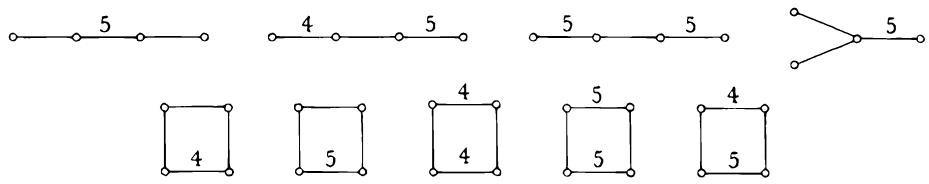
\includegraphics[keepaspectratio]{images/part001_8fab2eba.jpg}}

\begin{enumerate}
\def\labelenumi{\alph{enumi})}
\setcounter{enumi}{1}
\tightlist
\item
  对秩 5 回答同样的问题，其清单由下列五个图组成：
\end{enumerate}

\pandocbounded{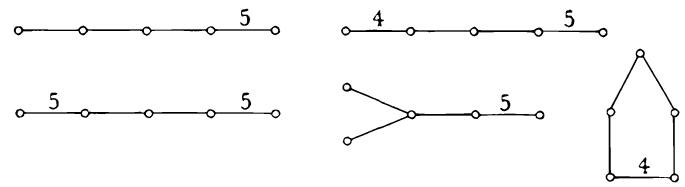
\includegraphics[keepaspectratio]{images/part001_6b3cac07.jpg}}

\begin{enumerate}
\def\labelenumi{\alph{enumi})}
\setcounter{enumi}{2}
\tightlist
\item
  证明不存在秩 \(\geqslant 6\) 的紧双曲型图。*
\end{enumerate}

\begin{enumerate}
\def\labelenumi{\arabic{enumi})}
\setcounter{enumi}{15}
\tightlist
\item
  *证明：任何有一条系数为 6 的棱的、秩 \(\geqslant 4\) 的双曲型 Coxeter 图都同构于下列十一个图之一（它们是非紧的且秩为 4）：
\end{enumerate}

\pandocbounded{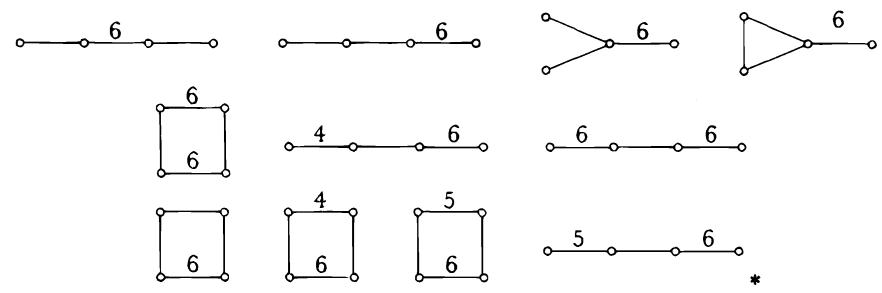
\includegraphics[keepaspectratio]{images/part001_2926a96c.jpg}}

\begin{enumerate}
\def\labelenumi{\arabic{enumi})}
\setcounter{enumi}{16}
\tightlist
\item
  *证明：更高秩的双曲 Coxeter 图是下列三个图（它们的秩为 10）：
\end{enumerate}

\pandocbounded{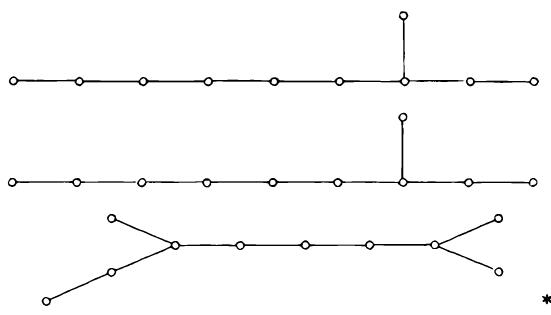
\includegraphics[keepaspectratio]{images/part001_3a8f46b0.jpg}}

¶ 18) 假设 (W,S) 是双曲型的，且 W 使 E 的一个格 \(\Gamma\) 稳定。设 G 是 \(B_{M}\) 的正交群，设 \(G(\Gamma)\) 是元素 \(g \in G\)（满足 \(g\Gamma = \Gamma\)）组成的子群。证明 \(G(\Gamma)\) 是 G 的离散子群。证明 W 是 \(G(\Gamma)\) 的有限指数子群（利用 W\textbackslash G 的测度有限这一事实）。

*若 (W, S) 实际上是紧双曲型的，证明相应的 Coxeter 图同构于下列图之一（使用 Exercs. 4, 6 与 15）：

\pandocbounded{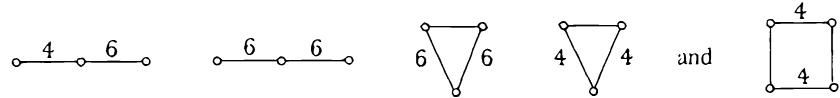
\includegraphics[keepaspectratio]{images/part001_0d92fd3d.jpg}}

证明与 Exerc. 16 的图（最后四个除外）相应的群都使一个格稳定（使用 Exerc. 6 的方法）。*

\begin{enumerate}
\def\labelenumi{\arabic{enumi})}
\setcounter{enumi}{18}
\tightlist
\item
  设 \((W,S)\) 是与图
\end{enumerate}

\pandocbounded{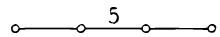
\includegraphics[keepaspectratio]{images/part001_8b3dcc37.jpg}}

相应的 Coxeter 系统。它是一个紧双曲型的系统（cf.~Exerc. 15）。型 \(B_{M}\) 关于基 \((e_{s})\) 的系数属于域 \(\mathbf{Q}(\sqrt{5})\) 中由该域的在 Z 上整的元素组成的子环 A。

\begin{enumerate}
\def\labelenumi{\alph{enumi})}
\item
  设 \(\sigma\) 是 \(K\) 到 \(\mathbf{R}\) 中的、把 \(\sqrt{5}\) 映为 \(-\sqrt{5}\) 的嵌入。证明 \(\sigma(B_M)\)（型 \(B_M\) 在 \(\sigma\) 下的像）非退化且正。
\item
  设 G 是 \(B_{M}\) 的正交群，\(G_{\sigma}\) 是 \(\sigma(B_{M})\) 的正交群。设 \(G_{A}\) 是 G 中由关于 \((e_{s})\) 的矩阵系数在 A 中的元素组成的子群。证明 \(G_{A}\) 可与 \(G \times G_{\sigma}\) 的一个离散子群等同，然后利用 a) 证明 \(G_{A}\) 是 G 的离散子群。
\item
  证明 W 是 \(G_{A}\) 的一个有限指数子群。
\end{enumerate}

\(d)\) 对 Exerc. 15 中的其余图证明类似的结果（域 \(\mathbf{Q}(\sqrt{5})\) 有时换成 \(\mathbf{Q}(\sqrt{2})\)），但下面的图除外：

\pandocbounded{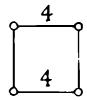
\includegraphics[keepaspectratio]{images/part001_99b486d1.jpg}}

即 Exerc. 18 中处理的图，以及图 \(^{8}\)

\pandocbounded{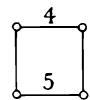
\includegraphics[keepaspectratio]{images/part001_2a5e784a.jpg}}

¶ 20) 对 S 的每个子集 \(\{s, s'\}\)（满足 \(m(s, s') = \infty\)），设 \(r(s, s')\) 是一个实数 \(\leqslant -1\)。给 E 赋以双线性型 \(\mathbf{B}_r\)，使得

\[
\begin{array}{l l} \mathrm{B} _ {r} (e _ {s}, e _ {s ^ {\prime}}) = \mathrm{B} _ {\mathrm{M}} (e _ {s}, e _ {s ^ {\prime}}) = - \cos \frac {\pi}{m (s , s ^ {\prime})} & \text {if} m (s, s ^ {\prime}) \neq \infty \\ \mathrm{B} _ {r} (e _ {s}, e _ {s ^ {\prime}}) = r (s, s ^ {\prime}) & \text {if} m (s, s ^ {\prime}) = \infty . \end{array}
\]

与 \(B_{M}\) 的情形一样，我们定义反射 \(\sigma_{s}\)，它以 \(e_{s}\) 为向量，且使型 \(B_{r}\) 不变。

\begin{enumerate}
\def\labelenumi{\alph{enumi})}
\item
  证明存在唯一的同态 \(\sigma_r: \mathbf{W} \to \mathbf{GL}(\mathbf{E})\)，使得 \(\sigma_r(g_s)\) 等于上面定义的反射 \(\sigma_s\)。
\item
  证明 Prop. 4、Th. 1 及其诸系、以及 Lemma 1 中的断言对 \(\sigma_r\) 仍然成立。
\end{enumerate}

\exercisesection{§ 5 的习题}

\begin{enumerate}
\def\labelenumi{\arabic{enumi})}
\item
  确定一个有限二面体群的对称不变元代数（就其 2 维典范表示而言，cf.~§4, no. 2）。
\item
  设 A 是一个主理想环，E 是一个有限秩 l 的自由 A-模，G 是 \(\mathbf{GL}(\mathbf{E})\) 的一个有限子群。假设：
\end{enumerate}

\begin{enumerate}
\def\labelenumi{(\roman{enumi})}
\item
  若 \(q = \operatorname{Card}(G)\)，则元素 \(q.1\)（\(A\) 中的元素）可逆。
\item
  G 由 E 中的伪反射生成（即由使 \((s - 1)(E)\) 是 E 的一个单生成子模的元素 s 生成，cf.~§2, Exerc. 1。）
\end{enumerate}

设 \(\mathbf{S}(\mathrm{E})\) 是 \(\mathrm{E}\) 的对称代数，\(\mathbf{S}(\mathrm{E})^{\mathrm{G}}\) 是 \(\mathbf{S}(\mathrm{E})\) 中由在 \(\mathrm{G}\) 下不变的元素组成的子代数。证明：对从 \(\mathrm{A}\) 到域 \(k\) 中的任何同态，\(\mathbf{S}(\mathrm{E})^{\mathrm{G}} \otimes k\) 可与 \(\mathbf{S}(\mathrm{E} \otimes k)^{\mathrm{G}}\) 等同。由此，应用 Th. 4 推出，\(\mathbf{S}(\mathrm{E})^{\mathrm{G}}\) 是 \(\mathrm{A}\) 上的一个分次多项式代数。

¶ 3) 设 K 是一个特征为零的域，V 是 K 上一个有限维 l 的向量空间，G 是 GL(V) 的一个由伪反射生成的子群。置 q = Card(G)；用 S（相应地，L）表示 V 的对称代数（相应地，外代数）。若 \(x \in V\)，用 x（相应地，\(x'\)）表示它在 S（相应地，L）中的典范像。

\begin{enumerate}
\def\labelenumi{\alph{enumi})}
\item
  设 \(E = S \otimes L\) 是 S 与 L 的张量积。证明 E 上存在唯一的导子 d，使得 \(dx = x'\) 且 \(dx' = 0\) 对所有 \(x \in V\) 成立。
\item
  设 \(S^{G}\) 是 G 的对称不变元代数，\(P_{1},\ldots,P_{l}\) 是 \(S^{G}\) 中使 \(S^{G}=K[P_{1},\ldots,P_{l}]\) 的齐次元素。对每个子集 \(I=\{i_{1},\ldots,i_{r}\}\)（\([1,l]\) 的、满足 \(i_{1}<\cdots<i_{r}\) 的子集），置
\end{enumerate}

\[
\omega_ {\mathrm{I}} = d \mathrm{P} _ {i _ {1}} \dots d \mathrm{P} _ {i _ {r}}.
\]

证明诸 \(\omega_{I}\) 在 S 上线性无关，且都属于 E 中由在 G 下不变的元素组成的子代数 \(E^{G}\)。由此推出，对所有 \(\omega \in E^{G}\)，存在 \(a, c_{I} \in S^{G}\)，其中 \(a \neq 0\)，使得

\[
a \omega = \sum_ {\mathrm{I}} c _ {\mathrm{I}} \omega_ {\mathrm{I}}.
\]

\(c)\) 证明 \(\mathrm{E}^{\mathrm{G}}\) 中包含在 \(S\otimes \bigwedge^{l}\mathrm{V}\) 中的每个元素都形如 \(c.dP_{1}\ldots dP_{l}\)，其中 \(c\in S^{\mathrm{G}}\)。（应用 Prop. 5。）

\begin{enumerate}
\def\labelenumi{\alph{enumi})}
\setcounter{enumi}{3}
\item
  证明诸 \(\omega_{I}\) 构成 \(S^{G}\)-模 \(E^{G}\) 的基。（用 b) 的记号，把关系式 \(a\omega = \sum_{I} c_{I}\omega_{I}\) 的两边乘以一个元素 \(\omega_{J}\)，并应用 c)；由此推出，若 I 是 J 的余集，则 a 整除 \(c_{I}\)；从而 \(^{9}\) 诸 \(\omega_{I}\) 生成 \(E^{G}\)。）
\item
  设 \(S_{n}\)（相应地，\(L_{m}\)）是 \(S\)（相应地，\(L\)）的 \(n\) 次（相应地，\(m\) 次）齐次分量。置
\end{enumerate}

\[
\begin{array}{r l r} & & {\mathrm{E} _ {n, m} = \mathrm{S} _ {n} \otimes \mathrm{L} _ {m}, \quad \mathrm{E} _ {n, m} ^ {\mathrm{G}} = \mathrm{E} ^ {\mathrm{G}} \cap \mathrm{E} _ {n, m}, \quad a _ {n, m} = \dim \mathrm{E} _ {n, m} ^ {\mathrm{G}},} \\ & & {a (\mathrm{X}, \mathrm{Y}) = \sum_ {n, m \geqslant 0} a _ {n, m} \mathrm{X} ^ {n} \mathrm{Y} ^ {m}.} \end{array}
\]

利用 \(d\) )，证明公式

\[
a (\mathrm{X}, \mathrm{Y}) = \prod_ {i = 1} ^ {l} \frac {1 + \mathrm{Y} . \mathrm{X} ^ {p _ {i} - 1}}{1 - \mathrm{X} ^ {p _ {i}}},
\]

其中 \(p_{i} = \deg(P_{i})\)。

\(f)\) 若 \(g \in \mathbf{G}\)，用 \(\operatorname{Tr}_{n,m}(g)\) 表示 \(\mathbf{E}_{n,m}\) 的、由 \(g\) 所定义的自同构的迹；置

\[
\operatorname{Tr} (\mathrm{X}, \mathrm{Y}) (g) = \sum_ {n, m \geqslant 0} \operatorname{Tr} _ {n, m} (g) \mathrm{X} ^ {n} \mathrm{Y} ^ {m}.
\]

证明

\[
\operatorname{Tr} (X, Y) (g) = \frac {\det (1 + Y g)}{\det (1 - X g)}.
\]

\begin{enumerate}
\def\labelenumi{\alph{enumi})}
\setcounter{enumi}{6}
\tightlist
\item
  设 \(q = \operatorname{Card}(\mathbf{G})\)。证明
\end{enumerate}

\[
\frac {1}{q} \sum_ {g \in G} \operatorname{Tr} (X, Y) (g) = a (X, Y),
\]

即

\[
\frac {1}{q} \sum_ {g \in G} \frac {\det (1 + Y g)}{\det (1 - X g)} = \prod_ {i = 1} ^ {l} \frac {1 + Y . X ^ {p _ {i} - 1}}{1 - X ^ {p _ {i}}}.
\]

（利用下列结果：若 \(\mathbf{G}\) 作用在一个有限维向量空间 \(\mathbf{E}\) 上，则 \(\mathbf{E}\) 中在 \(\mathbf{G}\) 下不变的元素所成空间的维数等于 \(\frac{1}{q}\sum_{g\in \mathbf{G}}\mathrm{Tr}_{\mathbf{E}}(g).\)）

当 Y = 0 时这个公式给出什么？

\begin{enumerate}
\def\labelenumi{\alph{enumi})}
\setcounter{enumi}{7}
\tightlist
\item
  对任何整数 \(p \geqslant 0\)，设 \(H_{p}\) 是 G 中以 1 为重数 p 的特征值的元素 \(g \in G\) 组成的集合。~设 \(h_{p} = \text{Card}(H_{p})\)。证明公式
\end{enumerate}

\[
\sum_ {p = 0} ^ {l} h _ {p} \mathbf {T} ^ {p} = \prod_ {i = 1} ^ {l} (p _ {i} - 1 + \mathbf {T}).
\]

（在上面的 \(g\) ) 中的公式里，把 \(Y\) 换成 \(-1 + T(1 - X)\)，然后在所得结果中置 \(X = 1\)。若 \(g \in H_p\)，则项 \(\operatorname{Tr}(X, Y)(g)\) 变成 \(T^p\)。）

¶ 4) *设 \(G _ {1} = \mathbf {S L} _ {3} (\mathbf {F} _ {2})\)。

\begin{enumerate}
\def\labelenumi{\alph{enumi})}
\item
  证明 \(\mathbf{G}_1\) 是一个 168 阶的非交换单群，含有 21 个 2 阶元素。
\item
  证明 \(G_{1}\) 的不可约复表示的次数是 1, 3, 3, 6, 7, 8。
\item
  设 \(\rho: \mathbf{G}_1 \to \mathbf{GL}_3(\mathbf{C})\) 是一个不可约表示 \(^{10}\)，它是 \(\mathbf{G}_1\) 的 3 次表示。若 \(y \in \mathbf{G}_1\) 是 2 阶的，证明 \(\operatorname{Tr}(\rho(y)) = -1\)。由此推出 \(-\rho(y)\) 是一个反射。
\item
  设 G 是 \(\mathbf{GL}_{3}(\mathbf{C})\) 中由诸元素 \(-\rho(y)\)（y 取遍 \(G_{1}\) 中的 2 阶元）生成的子群。证明 G 同构于 \(G_{1} \times \{1, -1\}\)，从而其阶为 336。
\item
  证明特征次数 \(k_{1}, k_{2}, k_{3}\)（\(\mathbf{G}\) 的对称不变元代数的特征次数）等于 4、6 与 14。（利用关系式 \(\prod_{i} k_{i} = 336\) 与 \(\sum_{i} (k_{i} - 1) = 21\)。）
\item
  证明 G 不是一个 Coxeter 群。*
\end{enumerate}

\begin{enumerate}
\def\labelenumi{\arabic{enumi})}
\setcounter{enumi}{4}
\tightlist
\item
  *设 \(K\) 是一个域，\(S = K[X_1, \ldots, X_n]\) 是 \(K\) 上的一个分次多项式代数，由代数无关的齐次元素 \(X_i\)（次数 \(> 0\)）生成。
\end{enumerate}

\begin{enumerate}
\def\labelenumi{\alph{enumi})}
\tightlist
\item
  设 \(Y_{1},\ldots,Y_{n}\) 是 S 中次数 \textgreater0 的齐次元素，\(R = K[Y_{1},\ldots,Y_{n}]\) 是 S 中由这些元素生成的子代数。证明下列性质等价：
\end{enumerate}

\begin{enumerate}
\def\labelenumi{(\roman{enumi})}
\item
  \((\mathrm{Y}_1,\dots ,\mathrm{Y}_n)\) 是一个 S-正则序列。
\item
  S 在 R 上是整的。
\item
  \(S\) 中由 \(Y_{1},\ldots ,Y_{n}\) 生成的理想在 \(S\) 中有有限余维数。
\item
  对任何扩张 \(\overline{\mathbf{K}}\)（\(\mathbf{K}\) 的扩张），方程组 \(Y_{i}(x_{1},\ldots ,x_{n}) = 0\)（\(1\leqslant i\leqslant n\)，\(x_{i}\in \overline{\mathbf{K}}\)）只有平凡解 \((0,\dots ,0)\)。
\end{enumerate}

\(((\mathrm{i}) \Longleftrightarrow (\mathrm{iii})\) 由 Macaulay 的一个定理得出（Commutative Algebra）；\((\mathrm{iii}) \Longleftrightarrow (\mathrm{iv})\) 由零点定理得出（Commutative Algebra, Chap. V, §3, no. 3, Prop. 2）；(ii) \(\Longleftrightarrow (\mathrm{iii})\) 是容易的。）

若这些性质满足，证明诸 \(Y_{i}\) 在 K 上代数无关，且 S 是一个自由 R-模，其秩等于

\[
\frac {\prod_ {i} \deg (\mathrm{Y} _ {i})}{\prod_ {i} \deg (\mathrm{X} _ {i})}.
\]

\begin{enumerate}
\def\labelenumi{\alph{enumi})}
\setcounter{enumi}{1}
\tightlist
\item
  设 G 是分次代数 S 的一个有限自同构群，\(S^{G}\) 是它的不变元子代数，\(Y_{1},\ldots,Y_{n}\) 是 \(S^{G}\) 中满足上面条件 (i),\ldots, (iv) 的元素。证明 \(S^{G}=K[Y_{1},\ldots,Y_{n}]\) 当且仅当
\end{enumerate}

\[
\operatorname{Card} (\mathrm{G}) = \frac {\prod_ {i} \deg \left(\mathrm{Y} _ {i}\right)}{\prod_ {i} \deg \left(\mathrm{X} _ {i}\right)}. *
\]

¶ 6) *设 n 是一个整数 ≥ 1，q 是一个素数的幂，K = F\_q，V = K\^{}n，G = GL(n, K)，G\_1 = SL(n, K)。把 G 与群 GL(V) 等同。此外，用 S 表示代数 S(V) = K{[}X\_1, \ldots, X\_n{]}，用 R（相应地，R\_1）表示 S 中由在 G（相应地，G\_1）下不变的元素组成的子代数。

\begin{enumerate}
\def\labelenumi{\alph{enumi})}
\tightlist
\item
  设 \(\mathbf{e} = (e_1, \ldots, e_n)\) 是一个整数序列 \(\geqslant 0\)。置
\end{enumerate}

\[
\mathrm{L} _ {\mathbf {e}} = \det (\mathrm{X} _ {i} ^ {q ^ {e _ {j}}}).
\]

这是 \(S\) 的一个元素。

证明

\[
g. \mathrm{L} _ {\mathbf {e}} = \det (g) \mathrm{L} _ {\mathbf {e}} \text {for all} g \in \mathrm{G}.
\]

（注意，若 \(g.X_i = \sum_j a_{ij} X_j\)，则 \(g.X_i^{q^e} = \sum_j a_{ij} X_j^{q^e}\)。）特别地，\(L_e\) 属于 \(R_1\)。

\begin{enumerate}
\def\labelenumi{\alph{enumi})}
\setcounter{enumi}{1}
\tightlist
\item
  设 \(j \in [1, n]\)。置
\end{enumerate}

\[
Z _ {j} = \prod_ {(a _ {i j})} (X _ {j} + \sum_ {i > j} a _ {i j} X _ {i}),
\]

其中乘积取遍 K 的元素的所有族 \((a_{ij})_{j < i\leqslant n}\)。设

\[
\mathrm{T} = \prod_ {j = 1} ^ {n} Z _ {j}.
\]

证明 T 整除所有 \(L_{e}\)。由此推出 \(T = L_{e_{n}}\)，其中 \(e_{n} = (0, 1, \ldots, n - 1)\)，且 T 在 \(G_{1}\) 下不变。

\begin{enumerate}
\def\labelenumi{\alph{enumi})}
\setcounter{enumi}{2}
\tightlist
\item
  用 \(\mathbf{e}_i\)（\(1 \leqslant i \leqslant n - 1\)）表示序列 \((0, 1, \ldots, i - 1, i + 1, \ldots, n)\)，并置 \(\mathrm{Y}_i = \mathrm{L}_{\mathbf{e}_i} / \mathrm{T}\)，cf.~b)。证明诸 \(\mathrm{Y}_i\) 属于 R 且 \(\deg(\mathrm{Y}_i) = q^n - q^i\)。
\end{enumerate}

\(d)\) 设 \(S' = K[X_1, \ldots, X_{n-1}]\)，并设 \(T', Y_1', \ldots, Y_{n-2}'\) 是 \(S'\) 中以与 \(T, Y_1, \ldots, Y_{n-1}\) 同样的方式（但把 \(n\) 换成 \(n-1\)）定义的元素。设 \(f: S \to S'\) 是由

\[
f \left(\mathrm{X} _ {i}\right) = \mathrm{X} _ {i} (1 \leqslant i \leqslant n - 1), f \left(\mathrm{X} _ {n}\right) = 0.
\]

定义的同态。证明

\[
f (\mathrm{T}) = 0, \quad f (\mathrm{Y} _ {1}) = \mathrm{T} ^ {\prime q (q - 1)}, \quad f (\mathrm{Y} _ {i}) = \mathrm{Y} _ {i - 1} ^ {\prime q} \quad \text{对} \quad 2 \leqslant i \leqslant n - 1.
\]

\begin{enumerate}
\def\labelenumi{\alph{enumi})}
\setcounter{enumi}{4}
\tightlist
\item
  证明族 \((T, Y_{1}, \ldots, Y_{n-1})\) 满足 Exerc. 5 的条件 (iv)。（设 \(x = (x_{1}, \ldots, x_{n})\) 是方程组 \((T, Y_{1}, \ldots, Y_{n-1})\) 在 K 的一个扩张 \(\overline{K}\) 中的一个零点。由于 x 是 T 的零点，诸 \(x_{i}\) 满足至少一个系数在 K 中的非平凡线性关系。必要时用 \(G_{1}\) 的一个元素变换 x，可以假设 \(x_{n} = 0\)。应用 d) 并对 n 用归纳法完成证明。）
\end{enumerate}

\(f)\) 证明 \(\mathbf{R}_1 = \mathbf{K}[\mathbf{T},\mathbf{Y}_1,\dots ,\mathbf{Y}_{n - 1}]\)，且 \(\mathrm{T},\mathrm{Y}_1,\dots ,\mathrm{Y}_{n - 1}\) 代数无关（“Dickson 定理”——应用 e) 与 Exerc. 5，并注意 \(\mathbf{G}_1\) 的阶等于 \(\deg (\mathrm{T}) = \sum_{i}\deg (\mathrm{Y}_i)\)）。

\begin{enumerate}
\def\labelenumi{\alph{enumi})}
\setcounter{enumi}{6}
\tightlist
\item
  证明 \(R = K[T^{q-1}, Y_{1}, \ldots, Y_{n-1}]\)。
\end{enumerate}

¶ 7) *设 R 是一个正则局部环（Commutative Algebra, Chap. VIII, §5, no. 1），其极大理想为 m，剩余域为 k。设 G 是 R 的一个有限自同构群，\(R' = R^{G}\) 是 R 中由在 G 下不变的元素组成的子环。这是一个局部环，其极大理想为 \(m' = m \cap R'\)。假设：

\begin{enumerate}
\def\labelenumi{(\roman{enumi})}
\item
  \(R'\) 是诺特的，且 R 是一个有限型 \(R'\)-模。
\item
  复合映射 \(R'\to R\to k\) 是满射。
\end{enumerate}

置 \(V = \mathfrak{m} / \mathfrak{m}^2\)；这是一个 \(k\)-向量空间。\(G\) 在 \(R\) 上的作用定义了一个同态 \(\varepsilon : G \to \mathbf{GL}(V)\)。

\begin{enumerate}
\def\labelenumi{\alph{enumi})}
\item
  设 \(\mathfrak{p}\) 是 \(R\) 的一个高度为 1 的素理想（Commutative Algebra, Chap. VII, §1, no. 6），\(s \in G\) 满足 \(s(\mathfrak{p}) = \mathfrak{p}\) 且 \(s\) 平凡地作用在 \(R / \mathfrak{p}\) 上。证明 \(\varepsilon(s)\) 是 \(V\) 的一个伪反射。（注意 \(\mathfrak{p}\) 在 \(\mathfrak{m} / \mathfrak{m}^2\) 中的像的维数是 0 或 1。）
\item
  证明：若 \(R'\) 正则，则子群 \(\varepsilon(G)\)（\(\mathbf{GL}(V)\) 的子群）由伪反射生成。（设 H 是 G 中由其在 \(\varepsilon\) 下的像为伪反射的元素生成的子群，\(R^{H}\) 是 R 中由在 H 下不变的元素组成的子环。利用 a) 证明：\(R'\) 的任何高度为 1 的素理想都不在 \(R^{H}\) 中分歧；利用 \(R^{H}\) 是整闭的这一事实，借助纯性定理 \(^{11}\) 推出 \(R' = R^{H}\)，从而 H = G。）
\item
  现在设 \(\mathbf{G}\) 的阶与 \(k\) 的特征互素。证明 \(\varepsilon\) 是单射。
\end{enumerate}

设 \((\mathfrak{m}_{n}^{\prime})\) 是 \(R^{\prime}\) 的、由 R 的 m-进滤链 \((\mathfrak{m}^{n})\) 诱导的滤链，并设

\[
i: \mathrm{gr} (\mathrm{R} ^ {\prime}) \to \mathrm{gr} (\mathrm{R})
\]

是从 \(R'\) 的相伴分次代数到 R 的相伴分次代数的典范同态（Commutative Algebra, Chap. III, §2）。证明 i 是单射，且它的像是子环 \(\mathrm{gr}(R)^{\mathrm{G}}\)，即 \(\mathrm{gr}(R)\) 中由在 G 下不变的元素组成的子环。

\(d)\) 沿用 \(c\) ) 的假设与记号，并进一步假设 \(\varepsilon (\mathbf{G})\) 由伪反射生成。若 \(l = \dim V\)，设 \(\mathrm{P}_1,\ldots ,\mathrm{P}_l\) 是 \(k\)-代数 \(\mathrm{gr}(R)^{\mathrm{G}}\) 的代数无关的齐次生成元（由 Th. 4 以及 \(\mathrm{gr}(R)\) 可与 V 的对称代数等同这一事实，这样的元素存在）；设 \(p_1,\ldots ,p_l\) 是它们的次数。由 \(c\) )，可以找到 \(x_{i}\in \mathfrak{m}_{p_{i}}^{\prime}\) 使得 \(\mathrm{gr}(x_i) = \mathrm{P}_i\)。证明诸 \(x_{i}\) 生成理想 \(\mathfrak{m}'\)，并由此推出 \(R'\) 是正则的。*

¶ 8) *设 V 是域 K 上一个有限维向量空间，S 是 V 的对称代数，G 是 GL(V) 的一个有限子群。假设代数 \(S^G\)（\(G\) 的对称不变量组成的代数）是一个分次多项式代数。

\begin{enumerate}
\def\labelenumi{\alph{enumi})}
\tightlist
\item
  设 u 是 V 的对偶 \(V^{*}\) 的一个元素，\(G_{u}\) 是 G 中由使 u 不变的元素组成的子群。证明 \(G_{u}\) 由伪反射生成。（线性型 u 可扩张为一个同态 \(f_{u}: S \to K\)。若用 \(S_{u}\) 表示 S 关于 \(f_{u}\) 的核的局部环，则环 \(S_{u}\) 是正则的。把 Exerc. 7 b) 应用于 \(G_{u}\)（把它视为 \(S_{u}\) 的自同构群），即得结论。）
\end{enumerate}

特别地，G 由伪反射生成。

\begin{enumerate}
\def\labelenumi{\alph{enumi})}
\setcounter{enumi}{1}
\tightlist
\item
  设 A 是 \(V^{*}\) 的一个子集，\(G_{A} = \bigcap_{u \in A} G_{u}\)。证明 \(G_{A}\) 由伪反射生成。（必要时扩张基域，可以假设 K 无限。证明在此情形下，存在由 A 生成的 \(V^{*}\) 的向量子空间中的一个元素 v，使得 \(G_{v} = G_{A}\)。对 \(v\) 应用 a) 即得结论。）
\end{enumerate}

\begin{enumerate}
\def\labelenumi{\arabic{enumi})}
\setcounter{enumi}{8}
\tightlist
\item
  设 V 是有限域 K（特征异于 2）上一个 4 维向量空间，Q 是 V 上一个指数为 2 的非退化二次型（Algebra, Chap. IX, §4, no. 2）。设 G = O(Q) 是这个型的正交群；这是一个由反射生成的有限群（loc. cit., §6, no. 4, Prop. 5）。
\end{enumerate}

\begin{enumerate}
\def\labelenumi{\alph{enumi})}
\item
  设 E 是 V 的一个极大全迷向子空间，\(G_{E}\) 是 G 中由使 \(g(x) = x\)（对所有 \(x \in E\)）的元素 g 组成的子群。证明 \(G_{E}\) 同构于 K 的加法群，且不含任何伪反射。
\item
  证明 G 的对称不变元代数不是一个分次多项式代数（利用前一习题）。
\end{enumerate}

\exercisesection{§ 6 的习题}

在下面的习题中（Exerc. 3 除外），假设与记号均取自 §6。

\begin{enumerate}
\def\labelenumi{\arabic{enumi})}
\item
  假设 W 不可约。设 c 是 W 的一个 Coxeter 变换，\(\Gamma\) 是 W 中由 c 生成的子群，\(\Delta\) 是与 H 的某个元素正交的单位向量组成的集合。证明 \(\Gamma\) 在 \(\Delta\) 中有 l 个轨道，且每个轨道有 h 个元素。（按 Chap. VI, §1, no. 11 的 Prop. 33 的证明方式论证。）
\item
  假设 W 不可约。设 C 是相对于 W 的一个室，\((\mathrm{H}_{1},\ldots,\mathrm{H}_{l})\) 是它的墙，\(e_{i}\) 是与 \(H_{i}\) 正交的一个非零向量。假设 \(e_{1},\ldots,e_{r}\)（相应地，\(e_{r+1},\ldots,e_{l}\)）两两正交（cf.~no. 2）。对所有 \(u\in Z\)，定义 \(H_{u}\) 与 \(s_{u}\) 如下：\(H_{u}=H_{k}\)（若 \(u\equiv k\pmod{l}\)），且 \(s_{u}=s_{H_{u}}\)。
\end{enumerate}

\begin{enumerate}
\def\labelenumi{\alph{enumi})}
\item
  证明 \(\mathfrak{H}\) 的元素正是诸 \(s_1 s_2 \ldots s_{u-1} H_u\)，其中 \(u = 1, 2, \ldots, lh/2\)。
\item
  设 \(s' = s_1 \ldots s_r\)，\(s'' = s_{r+1} \ldots s_l\)，于是 \(c = s's''\) 是与有序室 C 相伴的 Coxeter 变换。设 \(w_0\) 是 W 中把 C 变到 -C 的元素（cf.~§4, Exerc. 2）。证明：若 \(h\) 为奇数，则
\end{enumerate}

\[
w _ {0} = \underbrace {s ^ {\prime} s ^ {\prime \prime} s ^ {\prime} \ldots s ^ {\prime \prime} s ^ {\prime}} _ {h \text {terms}} = \underbrace {s ^ {\prime \prime} s ^ {\prime} s ^ {\prime \prime} \ldots s ^ {\prime} s ^ {\prime \prime}} _ {h \text {terms}} = s ^ {\prime \prime} c ^ {(h - 1) / 2} = c ^ {(h - 1) / 2} s ^ {\prime}.
\]

\begin{enumerate}
\def\labelenumi{\alph{enumi})}
\setcounter{enumi}{2}
\tightlist
\item
  置 \(S = \{s_1, \ldots, s_l\}\)。偶 (W,S) 是一个 Coxeter 系统。若 \(w \in W\)，用 \(l_S(w)\) 表示 \(w\) 关于 S 的长度（Chap. IV, §1, no. 1）。证明
\end{enumerate}

\[
l _ {\mathrm{S}} (s ^ {\prime}) = r, l _ {\mathrm{S}} (s ^ {\prime \prime}) = l - r, l _ {\mathrm{S}} (c) = l.
\]

在 b) 的假设下，由此推出

\[
l _ {\mathrm{S}} (w _ {0}) \leqslant r + \frac {h - 1}{2} l \text { and } l _ {\mathrm{S}} (w _ {0}) \leqslant (l - r) + \frac {h - 1}{2} l.
\]

另一方面，证明 \(l_{S}(w_0) = \mathrm{Card}(\mathfrak{H}) = hl / 2\)（使用 Chap. IV, §1 的 Exerc. 22）。由此推出 \(r = l / 2\)，且 \((s_1, s_2, \ldots, s_{lh / 2})\) 是 \(w_0\) 的一个约化分解。

\(d)\) 证明：若 \(h\) 为偶数，则 \((s_1,\ldots ,s_{lh / 2})\) 是 \(w_{0} = c^{h / 2}\) 的一个约化分解。（方法同上。）

¶ 3) 设 K 是一个交换环，E 是一个以 \((e_1, \ldots, e_l)\) 为基的自由 K-模，\(f_1, \ldots, f_l\) 是 E 的对偶中的元素。置 \(a_{ij} = f_i(e_j)\)。若 \(1 \leqslant i \leqslant l\)，设 \(s_i\) 是伪反射 \(s_{e_i, f_i}\)（\S 2, Exerc. 1）。则

\[
s _ {i} (e _ {j}) = e _ {j} - a _ {i j} e _ {i}.
\]

置 \(c = s_1 \ldots s_l\)，\(z_i = c(e_i)\)。

\begin{enumerate}
\def\labelenumi{\alph{enumi})}
\tightlist
\item
  对 \(1 \leqslant i, k \leqslant l\)，置
\end{enumerate}

\[
y _ {i} ^ {k} = s _ {1} \dots s _ {k} (e _ {i}) \text { and } y _ {i} = s _ {1} \dots s _ {i - 1} (e _ {i}) = y _ {i} ^ {i - 1}.
\]

于是 \(y_{i}^{0} = e_{i}\)，\(y_{i}^{l} = z_{i}\)。

证明

\[
y _ {i} ^ {k - 1} - y _ {i} ^ {k} = a _ {k i} y _ {k}.
\]

由此推出公式

\[
e _ {i} = y _ {i} + \sum_ {k <   i} a _ {k i} y _ {k}
\]

\[
z _ {i} = y _ {i} - \sum_ {k \geqslant i} a _ {k i} y _ {k}.
\]

\begin{enumerate}
\def\labelenumi{\alph{enumi})}
\setcounter{enumi}{1}
\tightlist
\item
  设 C 是 \(c\) 关于基 \((e_i)\) 的矩阵。设 \(U = (u_{ij})\) 与 \(V = (v_{ij})\) 是由下式定义的矩阵
\end{enumerate}

\[
u _ {i j} = \left\{ \begin{array}{l l} a _ {i j} & \text { if } i <   j \\ 0 & \text { otherwise, } \end{array} \right. v _ {i j} = \left\{ \begin{array}{l l} 0 & \text { if } i <   j \\ a _ {i j} & \text { otherwise. } \end{array} \right.
\]

矩阵 \(\mathrm{I} + \mathrm{U}\) 可逆且行列式为 1。证明

\[
\mathrm{C} = (\mathrm{I} - \mathrm{V}) (\mathrm{I} + \mathrm{U}) ^ {- 1}.
\]

由此推出

\[
\det (\lambda I - C) = \det ((\lambda - 1) I + V + \lambda U),
\]

换句话说

\[
\det (\lambda \mathrm{I} - \mathrm{C}) = \left| \begin{array}{c c c c c} (\lambda - 1) + a _ {1 1} & \lambda a _ {1 2} & \lambda a _ {1 3} & \dots & \lambda a _ {1 l} \\ a _ {2 1} & \lambda (\lambda - 1) + a _ {2 2} & \lambda a _ {2 3} & \dots & \lambda a _ {2 l} \\ a _ {3 1} & a _ {3 2} & (\lambda - 1) + a _ {3 3} & \dots & \lambda a _ {3 l} \\ \vdots & \vdots & \vdots & \ddots & \vdots \\ a _ {l 1} & a _ {l 2} & a _ {l 3} & \dots & (\lambda - 1) + a _ {l l} \end{array} \right|.
\]

\begin{enumerate}
\def\labelenumi{\alph{enumi})}
\setcounter{enumi}{2}
\tightlist
\item
  设 \(\Gamma = (\mathrm{I},\mathrm{S})\) 是这样的图：其顶点集为 \(\mathrm{I} = [1,l]\)，其棱集 S 是 I 的二元子集 \(\{i,j\}\)（满足 \(a_{ij}\neq 0\) 或 \(a_{ji}\neq 0\)）组成的集合。若 \(\alpha = \{i,j\}\) 属于 S，用 \(\sigma_{\alpha}\) 表示 \(i\) 与 \(j\) 的对换（视为对称群 \(\mathrm{S_I}\) 的元素），并置 \(a_{\alpha} = -a_{ij}a_{ji}\)。
\end{enumerate}

设 \(\mathfrak{B}\) 是 \(S\) 中由顶点两两不交的棱组成的子集的集合。若 \(X \in \mathfrak{B}\)，用 \(C(X)\) 表示所有这样的 \(i \in I\)（它们不是 \(X\) 的任何棱的顶点）组成的集合，并置 \(\sigma_X = \prod_{\alpha \in X} \sigma_\alpha\)，\(a_X = \prod_{\alpha \in X} a_\alpha\)。

设 \(\sigma \in S_{I}\)，\(d_{\sigma}\) 是与 \(\sigma\) 对应的项（在 \((\lambda - 1)I + V + \lambda U\) 的行列式展开式中）。证明：若 \(\sigma\) 形如 \(\sigma_{X}\)，其中 \(X \in \mathfrak{B}\)，则

\[
d _ {\sigma} = a _ {X} \lambda^ {\operatorname{Card} (X)} \prod_ {i \in C (X)} (\lambda - 1 + a _ {i i}).
\]

现在假设 \(\Gamma\) 是一个森林（Chap. IV, Appendix, no. 3）。证明：若 \(\sigma \in S_l\) 不形如 \(\sigma_X\)（\(X \in \mathfrak{B}\)），则 \(d_{\sigma} = 0\)。由此推出公式

\[
\det (\lambda - c) = \sum_ {X \in \mathfrak {B}} a _ {X} \lambda^ {\operatorname{Card} (X)} \prod_ {i \in C (X)} (\lambda - 1 + a _ {i i}).
\]

\begin{enumerate}
\def\labelenumi{\alph{enumi})}
\setcounter{enumi}{3}
\tightlist
\item
  考虑多项式
\end{enumerate}

\[
P (X) = \left| \begin{array}{c c c c} X & a _ {1 2} & \ldots & a _ {1 l} \\ a _ {2 1} & X & \ldots & a _ {2 l} \\ \vdots & \vdots & \ddots & \vdots \\ a _ {l 1} & a _ {l 2} & \ldots & X \end{array} \right|.
\]

在 \(c\) ) 的假设之外，再加设 \(a_{ii} = 1\)（对所有 \(i\)）。证明在此情形下

\[
\det (\lambda^ {2} - c) = \lambda^ {l} P (\lambda + \lambda^ {- 1}).
\]

\begin{enumerate}
\def\labelenumi{\arabic{enumi})}
\setcounter{enumi}{3}
\tightlist
\item
  在 no. 1 的假设与记号下，用 \(n_{ij}\) 表示 \(s_{\mathrm{H}_i}s_{\mathrm{H}_j}\) 的阶，并置 \(a_{ij} = -2\cos \frac{\pi}{n_{ij}}\)。于是 \(a_{ii} = 2\)，且 \(a_{ij} \leqslant 0\)（若 \(i \neq j\)），cf.~§3。利用前一习题的方法证明 \(^{12}\)：
\end{enumerate}

\[
\left| \begin{array}{c c c c} X & a _ {1 2} & \ldots & a _ {1 l} \\ a _ {2 1} & X & \ldots & a _ {2 l} \\ \vdots & \vdots & \ddots & \vdots \\ a _ {l 1} & a _ {l 2} & \ldots & X \end{array} \right| = \prod_ {i = 1} ^ {l} (X - 2 \cos (\pi m _ {i} / h)),
\]

其中 \(m_{1},\ldots ,m_{l}\) 是 W 的指数。

\chapter{根系}

\section{根系}

在本节中，k 表示一个特征为零的域。从 no. 3 起，我们假设 k = R。

\subsection{根系的定义}

引理 1. 设 V 是 k 上的向量空间，R 是生成 V 的有限子集。对于每个满足 \(\alpha \in R\)、\(\alpha \neq 0\) 的元素，至多存在一个 V 的反射 s，使得 \(s(\alpha) = -\alpha\) 且 \(s(R) = R\) 。

设 G 为保持 R 不变的 V 的自同构群。由于 R 生成 V，G 同构于 R 的对称群的一个子群，因而是有限的。设 \(s, s'\) 是 V 的反射，满足 \(s(\alpha) = s'(\alpha) = -\alpha\)、\(s(R) = R\)、\(s'(R) = R\)。于是 \(t = ss'\) 属于 G，因而具有有限阶 m。另一方面，

\[
t (\alpha) = \alpha \text { and } t (x) \equiv x \bmod k \alpha \text { for   all } x \in V.
\]

因此，存在一个线性形式 \(f\)，定义在 \(V\) 上，使得

\[
t (x) = x + f (x) \alpha \text {   for   all   } x \in V
\]

且 \(f(\alpha) = 0\)。对 \(n\) 归纳可得

\[
t ^ {n} (x) = x + n f (x) \alpha \text {   for   all   } x \in V.
\]

取 \(n\) 等于 \(m\)，我们看到 \(mf(x) = 0\) 对所有 \(x \in V\) 成立，所以 \(f = 0\)、\(t = 1\) 且 \(s = s'\)。

定义 1. 设 V 是 k 上的向量空间，R 是 V 的子集。若满足下列条件，则称 R 是 V 中的一个根系：

(RS \(_{I}\) ) R 是有限的，不含 0，且生成 V。

(RS \(_{II}\) ) 对所有 \(\alpha \in \mathbb{R}\)，存在元素 \(\alpha^{\prime}\)，属于 V 的对偶空间 V \(^{*}\)，使得 \(\langle \alpha, \alpha^{\prime} \rangle = 2\)，并且反射 \(s_{\alpha, \alpha'}\)（cf.~Chap. V, § 2）保持 R 不变。

(RS \(_{III}\) ) 对所有 \(\alpha \in R\)，有 \(\alpha^{\sim}(R) \subseteq \mathbf{Z}\)。

由引理 1，反射 \(s_{\alpha, \alpha'}\)（从而线性形式 \(\alpha'\) 也）由 \(\alpha\) 唯一确定，因此 \((\mathrm{RS}_{\mathrm{III}})\) 有意义。置 \(s_{\alpha, \alpha'} = s_{\alpha}\)。于是 \(s_{\alpha}(x) = x - \langle \alpha', x \rangle \alpha\)，对所有 \(x \in V\) 成立。

R 的元素称为（所考虑系统的）根。V 的维数称为该系统的秩。

保持 R 不变的 V 的自同构称为 R 的自同构。它们构成有限群，记为 A(R)。由 \(s_{\alpha}\) 生成的 A(R) 子群称为 R 的 Weyl 群，记为 W(R)，或简记为 W。

注。1）设 \(k'\) 是 \(k\) 的扩域。将 V 典范地视为 \(V \otimes k'\) 的子集，将 \(V^*\) 视为 \(V^* \otimes k' = (V \otimes k')^*\) 的子集。则 R 是 \(V \otimes k'\) 中的根系，且 \(\alpha'\) 与此前相同。

引理 2. 设 R 是 V 中的根系。设 \((x|y)\) 是 V 上的非退化、在 W(R) 下不变的对称双线性型。利用此型将 V 与 \(V^{*}\) 等同。若 \(\alpha \in R\)，则 \(\alpha\) 非等方，且

\[
\alpha^ {\prime} = \frac {2 \alpha}{(\alpha | \alpha)}.
\]

这由 Chap. V, § 2, no. 3 的公式 (4) 得出。

命题 1. 设 \(\mathrm{V}_{\mathbf{Q}}\)（相应地，\(\mathrm{V}_{\mathbf{Q}}^{*}\)）是一个 \(\mathbf{Q}\) -向量子空间，由 \(\mathrm{V}\)（相应地，\(\mathrm{V}^{*}\)）中的 \(\alpha\)（相应地，\(\alpha^{-}\)）生成。于是 \(\mathrm{V}_{\mathbf{Q}}\)（相应地，\(\mathrm{V}_{\mathbf{Q}}^{*}\)）是 \(\mathbf{Q}\) -结构，定义在 \(\mathrm{V}\)（相应地，\(\mathrm{V}^{*}\)）上（Algebra, Chap. II, § 8, no. 1）。将典范双线性型限制在 \(\mathrm{V}_{\mathbf{Q}} \times \mathrm{V}_{\mathbf{Q}}^{*}\) 上（该型定义在 \(\mathrm{V} \times \mathrm{V}^{*}\) 上），得到把空间 \(\mathrm{V}_{\mathbf{Q}}, \mathrm{V}_{\mathbf{Q}}^{*}\) 各自与另一个空间的对偶等同的映射。集合 \(\mathbb{R}\) 是 \(\mathrm{V}_{\mathbf{Q}}\) 中的根系。

若 \(k = \mathbf{R}\) ，则存在 \(V\) 上在 \(W(R)\) 下不变的内积（Integration, Chap. VII, § 3, no. 1, Prop. 1）；引理 2 现在表明 \(\alpha^{-}\) 生成 \(V^{*}\) 。由注记 1，\(\alpha^{-}\) 同样生成 \(V^{*}\)（当 \(k = \mathbf{Q}\) 时）。现在转到一般情形。置 \(E = V_{\mathbf{Q}}\) 。由 \((RS_{III})\) ，每个 \(\alpha^{-}\) 将 \(E\) 映到 \(\mathbf{Q}\) ，因而定义元素 \(\tilde{\alpha}\) 为 \(E^{*}\) 中的一个元素。显然 \(R\) 是 \(E\) 中的根系，并且与 \(\alpha\) 对应的 \(E^{*}\) 中的元素是 \(\tilde{\alpha}\) 。由上文所述，\(\tilde{\alpha}\) 生成向量空间 \(E^{*}\) 。考虑典范同态 \(i: E \otimes_{\mathbf{Q}} k \to V\) 及其转置 \({}^{t}i: V^{*} \to E^{*} \otimes_{\mathbf{Q}} k\) 。由于 \(R\) 生成 \(V\) ，\({}^{t}i\) 是单射；但 \({}^{t}i\) 的像包含 \(\tilde{\alpha}\) ，所以 \({}^{t}i\) 是满射。由此最终得到 \(i\) 和 \({}^{t}i\) 都是同构。因而可以把 \(V\) 与 \(E \otimes k\) 等同，把 \(V^{*}\) 与 \(E^{*} \otimes k\) 等同，把 \(\alpha^{-}\) 与 \(\tilde{\alpha}\) 等同，并把 \(V_{\mathbf{Q}}^{*}\) 与 \(E^{*}\) 等同。于是，\(V_{\mathbf{Q}}\)（相应地，\(V_{\mathbf{Q}}^{*}\)）是 \(Q\) -结构，定义在 \(V\)（相应地，\(V^{*}\)）上。将典范双线性型限制在 \(V_{\mathbf{Q}} \times V_{\mathbf{Q}}^{*}\) 上（该型定义在 \(V \times V^{*}\) 上）后，可以与 \(E \times E^{*}\) 上的典范双线性型等同，命题得证。

注记。2）命题 1 将根系的研究归结为 \(k = \mathbf{Q}\) 的情形。注 1 又将其进一步归结为实向量空间 \(V_{\mathbf{R}} = V_{\mathbf{Q}} \otimes_{\mathbf{Q}} \mathbf{R}\) 中的根系研究。与这些不同系统相关的 Weyl 群可典范地等同。

\begin{enumerate}
\def\labelenumi{\arabic{enumi})}
\setcounter{enumi}{2}
\tightlist
\item
  由于 \(\alpha^{\sim}\) 生成 \(V^{*}\)，群 \(W(R)\)（视为 \(\mathbf{GL}(V_{\mathbf{R}})\) 的子群）是本质的（Chap. V, § 3, no. 7）。此外，Chap. V, § 3, no. 2 的 Th. 1 的 Cor. 表明，属于 \(W(R)\) 的唯一反射是 \(s_{\alpha}\)。
\end{enumerate}

命题 2. \(\alpha^{\vee}\) 在 \(V^{*}\) 中构成根系，并且 \(\alpha^{\vee} = \alpha\) 对所有 \(\alpha \in R\) 成立。

由命题 1，\(\alpha^{\prime}\) 满足 \((\mathrm{RS}_{\mathrm{I}})\)。由于 \(s_{\alpha, \alpha'}\) 是赋予子集 R 的向量空间 V 的自同构，\({}^{t}(s_{\alpha, \alpha'})^{-1}\) 保持由 \(\alpha'\) 构成的集合 R' 不变；但 \({}^{t}(s_{\alpha, \alpha'})^{-1} = s_{\alpha', \alpha}\)，这证明了 R' 满足 \((\mathrm{RS}_{\mathrm{II}})\)，且 \(\alpha' = \alpha\)。最后，\(\langle \alpha', \beta \rangle \in \mathbf{Z}\) 对所有 \(\alpha' \in \mathrm{R'}\) 和 \(\beta \in \mathrm{R}\) 成立，所以 R' 满足 \((\mathrm{RS}_{\mathrm{III}})\)。

集合 \(R^{-}\) 称为 R 的逆根系。映射 \(\alpha \mapsto \alpha^{-}\) 是从 R 到 \(R^{-}\) 的双射，称为从 R 到 \(R^{-}\) 的典范双射。注意，若 \(\alpha, \beta\) 是 R 的元素且 \(\alpha + \beta \in R\)，则一般而言 \((\alpha + \beta)^{-} \neq \alpha^{-} + \beta^{-}\)。

由于 \(s_{\alpha}(\alpha) = -\alpha\)，公理 (RSII) 表明 \(-R = R\)。显然 \((- \alpha)^{\sim} = -\alpha^{\sim}\)，且 \(-1 \in A(R)\)（但 \(-1 \in W(R)\) 并不总成立）。

等式 \({}^{t}(s_{\alpha,\alpha^{-}})^{-1}=s_{\alpha^{-},\alpha}\) 表明映射 \(u\mapsto{}^{t}u^{-1}\) 是从群 W(R) 到群 W(R \(^{*}\) ) 的同构。我们借助此同构将这两个群等同；换言之，认为 W(R) 同时作用于 V 和 V \(^{*}\)。A(R) 同理。

命题 3. 对 \(x, y \in V\) ，置

\[
(x | y) = \sum_ {\alpha \in R} \langle \alpha^ {\vee}, x \rangle \langle \alpha^ {\vee}, y \rangle .
\]

则 \((x|y)\) 是 \(\mathbf{V}\) 上的非退化对称双线性型，在 \(\mathbf{A}(\mathbb{R})\) 下不变。对 \(x, y \in \mathrm{V}_{\mathbf{Q}}\)，有 \((x|y) \in \mathbf{Q}\)。\((x|y)\) 的典范延拓到

\[
V _ {R} = V _ {Q} \otimes_ {Q} R
\]

是非退化且正定的。

显然 \((x|y)\) 是 V 上的对称双线性型。若 \(g\in \mathrm{A}(\mathbb{R})\)

\[
(g (x) | g (y)) = \sum_ {\alpha \in R} \left\langle {} ^ {t} g \left(\alpha^ {-}\right), x \right\rangle \left\langle {} ^ {t} g \left(\alpha^ {-}\right), y \right\rangle = (x | y)
\]

因为 \((^t g)(\mathbb{R}^\sim) = \mathbb{R}^\sim\)。若 \(x, y \in \mathrm{V}_{\mathbf{Q}}\)，则 \((x|y) \in \mathbf{Q}\) 由 \((\mathrm{RS}_{\mathrm{III}})\) 得出。若 \(z \in \mathrm{V}_{\mathbf{R}}\)，则 \((z|z) = \sum_{\alpha \in \mathbb{R}} \langle \alpha^\sim, z \rangle^2 \geqslant 0\)，且有 \((z|z) > 0\)，只要 \(z \neq 0\)（由命题 1），所以 \((x|y)\) 到 \(V_{R}\) 的典范延拓是正定且非退化的。因此，\((x|y)\) 限制到 \(V_{Q}\) 后是非退化的，从而 V 上的型 \((x|y)\) 是非退化的。

命题 4. (i) 设 X 是 R 的子集，设 \(V_{X}\) 是由 X 生成的 V 的向量子空间，设 \(V'_{X}\) 是 \(V^{*}\) 中的向量子空间，由 \(\alpha'\) 生成，其中 \(\alpha \in X\)。于是 V 是 \(V_{X}\) 与 \(V'_{X}\) 的正交补的直和，\(V^{*}\) 是 \(V'_{X}\) 与 \(V_{X}\) 的正交补的直和，并且 \(V'_{X}\) 与 \(V_{X}\) 的对偶等同。

\begin{enumerate}
\def\labelenumi{(\roman{enumi})}
\setcounter{enumi}{1}
\tightlist
\item
  \(R \cap V_{X}\) 是 \(V_{X}\) 中的根系，并且从 \(R \cap V_{X}\) 到其逆根系的典范双射等同于将映射 \(\alpha \mapsto \alpha^{-}\) 限制到 \(R \cap V_{X}\) 所得的映射。
\end{enumerate}

由注记 2，可假设 \(k = \mathbf{R}\)。利用命题 3 的对称双线性型将 \(V\) 与 \(V^*\) 等同。由引理 2，有 \(\alpha^{-} = \frac{2\alpha}{(\alpha|\alpha)}\) 对所有 \(\alpha \in R\) 成立（引理 2）。\(V\) 的每个向量子空间都是非等方的，命题现已显然。

推论。设 \(V_{1}\) 是 V 的一个向量子空间，设 \(V_{2}\) 是由 \(R \cap V_{1}\) 生成的向量子空间。则 \(R \cap V_{1}\) 是 \(V_{2}\) 中的根系。

这由将 (ii) 应用于 \(\mathrm{X} = \mathrm{R} \cap \mathrm{V}_1\) 得出。

对 \(\alpha, \beta \in \mathbb{R}\)，置

\[
\langle \alpha , \beta^ {\prime} \rangle = n (\alpha , \beta).\tag{1}
\]

于是

\[
n (\alpha , \alpha) = 2\tag{2}
\]

\[
n (- \alpha , \beta) = n (\alpha , - \beta) = - n (\alpha , \beta).\tag{3}
\]

由 \((\mathrm{RS}_{\mathrm{III}})\)

\[
n (\alpha , \beta) \in \mathbf {Z}.\tag{4}
\]

由 \(n(\alpha, \beta)\) 的定义，

\[
s _ {\beta} (\alpha) = \alpha - n (\alpha , \beta) \beta .\tag{5}
\]

公式 (1) 和命题 2 蕴含

\[
n (\alpha , \beta) = n \left(\beta^ {-}, \alpha^ {-}\right).\tag{6}
\]

设 \((x|y)\) 是 V 上的非退化、在 W(R) 下不变的对称双线性型（命题 3）。由引理 2，

\[
n (\alpha , \beta) = \frac {2 (\alpha | \beta)}{(\beta | \beta)}.\tag{7}
\]

于是

\[
n (\alpha , \beta) = 0 \Longleftrightarrow n (\beta , \alpha) = 0 \Longleftrightarrow (\alpha | \beta) = 0 \Longleftrightarrow s _ {\alpha} \text {   and   } s _ {\beta} \text {   commute.   (8) }
\]

\[
\text {   If   } (\alpha | \beta) \neq 0, \text {   then   } \frac {n (\beta , \alpha)}{n (\alpha , \beta)} = \frac {(\beta | \beta)}{(\alpha | \alpha)}.\tag{9}
\]

\subsection{根系的直和}

设 \(V\) 是 \(k\) 上的向量空间，且是向量空间族 \((V_i)_{1 \leqslant i \leqslant r}\) 的直和。将 \(V^*\) 与 \(V_i^*\) 的直和等同。对所有 \(i\)，设 \(R_i\) 是 \(V_i\) 中的根系。则 \(R = \bigcup_i R_i\) 是 \(V\) 中的根系，其逆根系为 \(R^- = \bigcup_i R_i^-\)；从 \(R\) 到 \(R^-\) 的典范双射对每个 \(i\) 都扩张了从 \(R_i\) 到 \(R_i^-\) 的典范双射。集合 \(R\) 称为根系 \(R_i\) 的直和。设 \(\alpha \in R_i\)。若 \(j \neq i\)，则 \(\alpha^-\) 的核包含 \(V_j\)，所以 \(s_\alpha\) 在 \(V_j\) 上诱导恒等映射；另一方面，\(k\alpha \subseteq V_i\)，所以 \(s_\alpha\) 保持 \(V_i\) 不变。这些说明表明，\(W(R)\) 可与 \(\prod_{i=1}^{r} W(R_i)\) 等同。

称根系 R 是不可约的，当且仅当 \(R \neq \varnothing\)，且 R 不是两个非空根系的直和。

命题 5. 设 V 是 k 上的向量空间，且 V 是向量空间 \(V_{1}, \ldots, V_{r}\) 的直和。设 R 是 V 中的根系。置 \(R_{i} = R \cap V_{i}\)。以下三个条件等价：

\begin{enumerate}
\def\labelenumi{(\roman{enumi})}
\item
  \(V_{i}\) 在 W(R) 下不变；
\item
  \(R \subseteq V_{1} \cup V_{2} \cup \cdots \cup V_{r};\)
\item
  对所有 \(i\)，\(\mathbb{R}_i\) 是 \(\mathrm{V}_i\) 中的根系，且 \(\mathbb{R}\) 是 \(\mathbb{R}_i\) 的直和。
\item
  \(\Longrightarrow\) (i)：这由本号开头所述得到。
\item
  \(\Longrightarrow\) (ii)：假设 \(V_{i}\) 在 \(W(R)\) 下不变。设 \(\alpha \in R\)，并设 H 是 \(\alpha\) 的核。由 Chap. V, § 2, no. 2 的 Prop. 3，每个 \(V_{i}\) 都是 H 的一个子空间与 \(k\alpha\) 的一个子空间之和。因此某个 \(V_{i}\) 包含 \(k\alpha\)，所以 \(\alpha \in V_{1} \cup V_{2} \cup \cdots \cup V_{r}\)。
\item
  \(\Longrightarrow\) (iii)：若条件 (ii) 满足，则 \(\mathbf{R}_i\) 生成 \(\mathbf{V}_i\) 对所有 \(i\) 成立，所以 \(\mathbf{R}_i\) 是 \(\mathbf{V}_i\) 中的根系（命题 4）。显然 \(\mathbf{R}\) 是 \(\mathbf{R}_i\) 的直和。
\end{enumerate}

推论。设 R 是 V 中的根系。以下条件等价：

\begin{enumerate}
\def\labelenumi{(\roman{enumi})}
\item
  R 不可约：
\item
  W(R)-模 V 是单的；
\item
  W(R)-模 V 是绝对单的。
\item
  \(\Longleftrightarrow\) (i)：这由命题 5 和 Maschke 定理（Chap. V, Appendix, Prop. 2）得到。
\item
  \(\Longleftrightarrow\) (ii)：这由 Chap. V, § 2, no. 1 的 Prop. 1 得到。
\end{enumerate}

命题 6. V 中的每个根系 R 都是一个不可约根系族 \((\mathrm{R}_{i})_{i\in I}\) 的直和，并且除指标集的一个双射外是唯一的。

\(R_{i}\) 的存在性由对 Card R 归纳证明：若 R 非空且可约，则 R 是两个根系 \(R'\)、\(R''\) 的直和，满足 \(Card R' < Card R\)、\(Card R'' < Card R\)，并且归纳假设适用于 \(R'\) 和 \(R''\)。为证明唯一性，只需证明：若 R 是 \(R'\) 与 \(R''\) 的直和，则每个 \(R_i\) 必然包含于 \(R'\) 或 \(R''\) 中。设 \(V', V'', V'_i, V''_i\) 是 V 中分别由 \(R', R'', R' \cap R_i, R'' \cap R_i\) 生成的向量子空间。由于和 \(V' + V''\) 是直和，和 \(V'_i + V''_i\) 也是直和。由于 \(R_i \subseteq R' \cup R''\)，\(R_i\) 是根系 \(R' \cap R_i\) 与 \(R'' \cap R_i\) 的直和；因此 \(R' \cap R_i = \varnothing\) 或 \(R'' \cap R_i = \varnothing\)，这就证明了所述断言。

\(R_{i}\) 称为 R 的不可约分支。对于任意非零标量 \(\lambda_{i}\)，\(\lambda_{i}R_{i}\) 的并集是 V 中的根系，其逆根系是 \(\lambda_{i}^{-1}R_{i}\) 的并集，并且其 Weyl 群为 \(\mathrm{W}(\mathrm{R})\)。

命题 7. 设 R 是 V 中的根系，(R \(_{i}\) ) 是其不可约分支族，V \(_{i}\) 是由 R \(_{i}\) 生成的 V 的向量子空间，B 是命题 3 中定义的 V 上的不变对称双线性型，B' 是 V 上在 W(R) 下不变的对称双线性型。则各 V \(_{i}\) 关于 B' 两两正交，并且对所有 i，B 和 B' 在 V \(_{i}\) 上的限制成比例。

若 \(v_{i} \in \mathrm{V}_{i}\)、\(v_{j} \in \mathrm{V}_{j}\)、\(i \neq j\)，且 \(w \in \mathrm{W}(\mathrm{R}_j)\)，则

\[
\mathrm{B} ^ {\prime} (v _ {i}, w (v _ {j})) = \mathrm{B} ^ {\prime} (v _ {i}, v _ {j}),
\]

这表明 \(w(v_{j}) - v_{j}\) 与 \(v_{i}\) 关于 \(B'\) 正交。由于 \(V_{j}\) 对 \(\mathrm{W}(\mathrm{R}_{j})\) 不可约，它由 \(w(v_{j}) - v_{j}\) 生成，因此它与 \(V_{i}\) 正交。

B 和 B' 在各个 \(V_{i}\) 上的限制成比例这一事实由 Chap. V, § 2, no. 1 的 Prop. 1 得到。

注。取一个 \(V_{R}\) 上在 \(W(R)\) 下不变的内积。于是可以谈论根的长度以及两个根之间的角。命题 7 表明，只要两个根属于 R 的同一不可约分支，这个角与内积的选择无关，两个根的长度之比也与内积的选择无关。

\subsection{两个根之间的关系}

回顾一下，从现在起我们假设 k = R。（将定义和结果推广到一般情形的任务留给读者，方法见第 1 号的注记 2。）

以下始终，R 表示向量空间 V 中的一个根系；并且 V 配备了一个在 W(R) 下不变的内积 \((x,y)\mapsto(x|y)\)，cf.~Prop. 3。

设 \(\alpha, \beta \in \mathbb{R}\)。由第 1 号的公式 (7)，

\[
n (\alpha , \beta) n (\beta , \alpha) = 4 \cos^ {2} (\widehat {\alpha , \beta}) \leqslant 4.\tag{10}
\]

因此，整数 \(n(\alpha,\beta)n(\beta,\alpha)\) 必须取 0、1、2、3、4 中的一个值。根据 Chap. V, § 2, no. 5 的 Prop. 6 的 Cor. 以及 Chap. V, § 4, no. 8 页上的脚注，我们看到，除交换 \(\alpha\) 与 \(\beta\) 外，唯一的可能性如下：

\[
1) \quad n (\alpha , \beta) = n (\beta , \alpha) = 0; \quad \widehat {(\alpha , \beta)} = \frac {\pi}{2}; \quad s _ {\alpha} s _ {\beta} \text {of order} 2;
\]

\[
2) \quad n (\alpha , \beta) = n (\beta , \alpha) = 1; \quad (\alpha , \beta) = \frac {\pi}{3}; \quad s _ {\alpha} s _ {\beta} \text {   of   order   } 3;
\]

\[
\parallel \alpha \parallel = \parallel \beta \parallel ;
\]

\[
3) \quad n (\alpha , \beta) = n (\beta , \alpha) = - 1;
\]

\[
\widehat {(\alpha , \beta)} = \frac {2 \pi}{3};
\]

\[
s _ {\alpha} s _ {\beta} \text {of order 3};
\]

\[
\| \alpha \| = \| \beta \|;
\]

\[
4) \quad n (\alpha , \beta) = 1, n (\beta , \alpha) = 2; \qquad \widehat {(\alpha , \beta)} = \frac {\pi}{4};
\]

\[
s _ {\alpha} s _ {\beta} \text {   of   order   4;   }
\]

\[
\parallel \beta \parallel = \sqrt {2} \parallel \alpha \parallel ;
\]

\[
5) \quad n (\alpha , \beta) = - 1, n (\beta , \alpha) = - 2;
\]

\[
\widehat {(\alpha , \beta)} = \frac {3 \pi}{4};
\]

\[
s _ {\alpha} s _ {\beta} \text {   of   order   4;   }
\]

\[
\parallel \beta \parallel = \sqrt {2} \parallel \alpha \parallel ;
\]

\[
6) \quad n (\alpha , \beta) = 1, n (\beta , \alpha) = 3;
\]

\[
\widehat {(\alpha , \beta)} = \frac {\pi}{6};
\]

\[
s _ {\alpha} s _ {\beta} \text {   of   order   } 6;
\]

\[
\parallel \beta \parallel = \sqrt {3} \parallel \alpha \parallel ;
\]

\[
7) \quad n (\alpha , \beta) = - 1, n (\beta , \alpha) = - 3;
\]

\[
\widehat {(\alpha , \beta)} = \frac {5 \pi}{6};
\]

\[
s _ {\alpha} s _ {\beta} \text {   of   order   6;   }
\]

\[
\parallel \beta \parallel = \sqrt {3} \parallel \alpha \parallel ;
\]

\begin{enumerate}
\def\labelenumi{\arabic{enumi})}
\setcounter{enumi}{7}
\item
  \(n(\alpha, \beta) = n(\beta, \alpha) = 2; \quad \alpha = \beta;\)
\item
  \(n(\alpha, \beta) = n(\beta, \alpha) = -2; \quad \alpha = -\beta;\)
\item
  \(n(\alpha, \beta) = 1\) , \(n(\beta, \alpha) = 4\) ; \(\beta = 2\alpha\) ;
\item
  \(n(\alpha, \beta) = -1\) , \(n(\beta, \alpha) = -4\) ; \(\beta = -2\alpha\) .
\end{enumerate}

特别地：

命题 8. (i) 若两个根成比例，则比例因子只能是 \(\pm 1, \pm \frac{1}{2}, \pm 2\)。

\begin{enumerate}
\def\labelenumi{(\roman{enumi})}
\setcounter{enumi}{1}
\tightlist
\item
  若 \(\alpha\) 和 \(\beta\) 是两个不成比例的根，且 \(\| \alpha \| \leqslant \| \beta \|\)，则 \(n(\alpha, \beta)\) 取 \(0, 1, -1\) 中的一个值。
\end{enumerate}

若根 \(\alpha \in \mathbb{R}\) 满足 \(\frac{1}{2}\alpha \notin \mathbb{R}\)，则称 \(\alpha\) 为不可分根。

定理 1. 设 \(\alpha, \beta\) 是两个根。

\begin{enumerate}
\def\labelenumi{(\roman{enumi})}
\item
  若 \(n(\alpha, \beta) > 0\)，则 \(\alpha - \beta\) 是根，除非 \(\alpha = \beta\)。
\item
  若 \(n(\alpha, \beta) < 0\)，则 \(\alpha + \beta\) 是根，除非 \(\alpha = -\beta\)。
\end{enumerate}

若 \(n(\alpha, \beta) > 0\)，则根据上面的列表，可能性如下：

\begin{enumerate}
\def\labelenumi{\arabic{enumi})}
\item
  \(n(\alpha, \beta) = 1\)；于是 \(\alpha - \beta - s_{\beta}(\alpha) \in \mathbb{R}\)；
\item
  \(n(\beta, \alpha) = 1\)；于是 \(\beta - \alpha = s_{\alpha}(\beta) \in \mathbb{R}\)，所以 \(\alpha - \beta \in \mathbb{R}\)；
\item
  \(\beta = \alpha\) .
\end{enumerate}

这证明了 (i)，而 (ii) 由将 \(\beta\) 换成 \(-\beta\) 得到。

推论。设 \(\alpha\) 和 \(\beta\) 是两个根。

\begin{enumerate}
\def\labelenumi{(\roman{enumi})}
\item
  若 \((\alpha |\beta) > 0\)，则 \(\alpha - \beta\) 是根，除非 \(\alpha = \beta\)。
\item
  若 \((\alpha |\beta) < 0\)，则 \(\alpha + \beta\) 是根，除非 \(\alpha = -\beta\)。
\item
  若 \(\alpha - \beta \notin R \cup \{0\}\) 且 \(\alpha + \beta \notin R \cup \{0\}\)，则 \((\alpha | \beta) = 0\)。
\end{enumerate}

断言 (i) 和 (ii) 由 Th. 1 以及第 1 号的公式 (7) 得到。断言 (iii) 由 (i) 和 (ii) 得到。

可能有 \(\alpha + \beta \in \mathbb{R}\) 且 \((\alpha|\beta) = 0\)（cf.~Plate X, System \(B_{2}\)）。当 \(\alpha - \beta \notin \mathbb{R} \cup \{0\}\) 且 \(\alpha + \beta \notin \mathbb{R} \cup \{0\}\) 时，称 \(\alpha\) 与 \(\beta\) 强正交。

命题 9. 设 \(\alpha\) 和 \(\beta\) 是两个不成比例的根。

\begin{enumerate}
\def\labelenumi{(\roman{enumi})}
\item
  整数 \(j\) 的集合 I（使得 \(\beta + j\alpha\) 是根）是包含 0 的区间 \([-q, p]\)，位于 \(\mathbf{Z}\) 中。
\item
  设 \(S\) 是由 \(\beta + j\alpha\)（其中 \(j \in I\)）组成的集合。于是，
\end{enumerate}

\[
s _ {\alpha} (S) = S \text { and } s _ {\alpha} (\beta + p \alpha) = \beta - q \alpha .
\]

\begin{enumerate}
\def\labelenumi{(\roman{enumi})}
\setcounter{enumi}{2}
\tightlist
\item
  \(p - q = -n(\beta, \alpha)\)。
\end{enumerate}

显然，\(0 \in I\)。设 \(p\)（相应地，\(-q\)）是 \(I\) 的最大（相应地，最小）元素。若不是区间 \([-q, p]\) 中的所有整数都属于 \(I\)，则存在两个整数 \(r, s\) 在区间 \([-q, p]\) 中，具有以下性质：\(s > r + 1\)、\(s \in I\)、\(r \in I\)，并且 \(r + k \notin I\) 对 \(1 \leqslant k \leqslant s - r - 1\) 成立。按照 Th. 1 的 Cor. 的记号，有 \((\alpha|\beta + s\alpha) \leqslant 0\)、\((\alpha|\beta + r\alpha) \geqslant 0\)，这不可能，因为

\[
(\alpha | \beta + s \alpha) \leqslant 0 > (\alpha | \beta + r \alpha).
\]

这证明了 (i)。

我们有 \(s_{\alpha}(\beta + j\alpha) = \beta - n(\beta, \alpha)\alpha - j\alpha = \beta + j'\alpha\)，其中 \(j' = -j - n(\beta, \alpha)\)。因此 \(s_{\alpha}(S) \subseteq S\)，从而 \(s_{\alpha}(S) = S\)。现在 \(j \mapsto -j - n(\beta, \alpha)\) 是从 I 到 I 的递减双射。于是，\(j' = -q\) 在 \(j = p\) 时成立，从而 \(-q = -p - n(\beta, \alpha)\)。这证明了 (ii) 和 (iii)。

集合 S 称为 \(\alpha\)-根链，它由 \(\beta\) 定义；\(\beta - q\alpha\) 是其起点，\(\beta + p\alpha\) 是其终点，而 \(p + q\) 是其长度。

推论。设 S 是根的 \(\alpha\)-链，\(\gamma\) 是 S 的起点。S 的长度为 \(-n(\gamma,\alpha)\)；它等于 0、1、2 或 3。

第一个断言由将 \(\beta = \gamma\) 应用于命题 9 的 (iii)，并利用 \(q = 0\) 这一事实得到。

另一方面，由于 \(\gamma\) 与 \(\alpha\) 不成比例，本号开头给出的列表表明 \(|n(\gamma,\alpha)|\leqslant3\)，故得出该推论。

注。沿用上述记号。则：

\begin{enumerate}
\def\labelenumi{\arabic{enumi})}
\item
  若 S 的长度为 0，则 \((\alpha |\gamma) = 0\)。
\item
  若 \(S\) 的长度为 1，则 \(n(\gamma, \alpha) = -1\)，且有三种情形：
\end{enumerate}

\[
n (\alpha , \gamma) = - 1, \quad (\alpha | \alpha) = (\gamma | \gamma), \quad (\alpha | \gamma) = - \frac {1}{2} (\alpha | \alpha), \quad \widehat {(\alpha , \gamma)} = \frac {2 \pi}{3}
\]

\[
n (\alpha , \gamma) = - 2, \quad (\alpha | \alpha) = 2 (\gamma | \gamma), \quad (\alpha | \gamma) = - \frac {1}{2} (\alpha | \alpha), \quad \widehat {(\alpha , \gamma)} = \frac {3 \pi}{4}
\]

\[
n (\alpha , \gamma) = - 3, \quad (\alpha | \alpha) = 3 (\gamma | \gamma), \quad (\alpha | \gamma) = - \frac {1}{2} (\alpha | \alpha), \quad (\widehat {\alpha , \gamma}) = \frac {5 \pi}{6}
\]

\pandocbounded{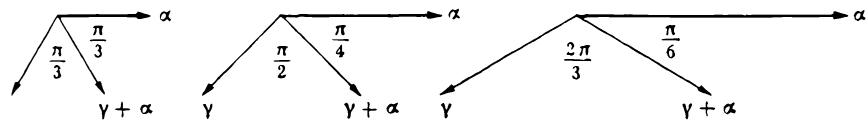
\includegraphics[keepaspectratio]{images/part001_d4d2d336.jpg}}

\begin{enumerate}
\def\labelenumi{\arabic{enumi})}
\setcounter{enumi}{2}
\tightlist
\item
  若 \(S\) 的长度为 2，则 \(n(\gamma, \alpha) = -2\)，因此
\end{enumerate}

\[
n (\alpha , \gamma) = - 1, (\alpha | \alpha) = \frac {1}{2} (\gamma | \gamma), (\alpha | \gamma) = - (\alpha | \alpha), \widehat {(\alpha , \gamma)} = \frac {3 \pi}{4}.
\]

\pandocbounded{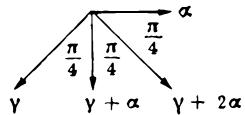
\includegraphics[keepaspectratio]{images/part001_f07fa75a.jpg}}

\begin{enumerate}
\def\labelenumi{\arabic{enumi})}
\setcounter{enumi}{3}
\tightlist
\item
  若 \(S\) 的长度为 3，则 \(n(\gamma, \alpha) = -3\)，因此
\end{enumerate}

\[
n (\alpha , \gamma) = - 1, (\alpha | \alpha) = \frac {1}{3} (\gamma | \gamma), (\alpha | \gamma) = - \frac {3}{2} (\alpha | \alpha), (\widehat {\alpha , \gamma}) = \frac {5 \pi}{6}.
\]

\pandocbounded{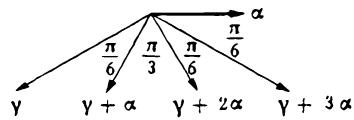
\includegraphics[keepaspectratio]{images/part001_9d247bec.jpg}}

我们将看到（Plate X, Systems \(A_{2}, B_{2}, G_{2}\)），所有这些情形实际上都能实现。

命题 10. 设 \(\alpha, \beta\) 是两个不成比例的根，且 \(\beta + \alpha\) 是一个根。设 \(p, q\) 是命题 9 中的整数。则

\[
\frac {(\beta + \alpha | \beta + \alpha)}{(\beta | \beta)} = \frac {q + 1}{p}.
\]

设 \(S\) 是 \(\alpha\)-链，由 \(\beta\) 定义，\(\gamma\) 是其起点；其长度 \(l\) 满足 \(\geqslant 1\)，因为 \(\beta + \alpha\) 是根。可能的情形如下：

\begin{enumerate}
\def\labelenumi{\arabic{enumi})}
\item
  \(l = 1\)；于是 \(\beta = \gamma, q = 0, p = 1, (\beta + \alpha | \beta + \alpha) = (\beta | \beta)\)。
\item
  \(l = 2\)，\(\beta = \gamma\)；于是 \(q = 0\)，\(p = 2\)，\((\beta + \alpha|\beta + \alpha) = \frac{1}{2} (\beta|\beta)\)。
\item
  \(l = 2, \beta = \gamma + \alpha\)；于是 \(q = 1, p = 1, (\beta + \alpha|\beta + \alpha) = 2(\beta|\beta)\)。
\item
  \(l = 3, \beta = \gamma\)；于是 \(q = 0, p = 3, (\beta + \alpha | \beta + \alpha) = \frac{1}{3} (\beta | \beta)\)。
\item
  \(l = 3, \beta = \gamma + \alpha\)；于是 \(q = 1, p = 2, (\beta + \alpha|\beta + \alpha) = (\beta|\beta)\)。
\item
  \(l = 3\)，\(\beta = \gamma + 2\alpha\)；于是 \(q = 2, p = 1\)，\((\beta + \alpha|\beta + \alpha) = 3(\beta|\beta)\)。
\end{enumerate}

每种情形都满足待证公式。

命题 11. 假设 R 不可约。设 \(\alpha\) 和 \(\beta\) 是满足 \(\| \alpha \| = \| \beta \|\) 的两个根。存在 \(g \in \mathrm{W}(\mathbb{R})\)，使得 \(g(\alpha) = \beta\)。

根 \(\alpha\) 在 W(R) 下的变换生成 V（no. 2, Cor. of Prop. 5）。因此存在 \(g \in \mathrm{W}(\mathbb{R})\)，使得 \((g(\alpha)|\beta) \neq 0\)。从现在起假设 \((\alpha|\beta) \neq 0\)。由第 1 号的公式 (9)，\(n(\alpha, \beta) = n(\beta, \alpha)\)。必要时将 \(\beta\) 换成 \(s_{\beta}(\beta) = -\beta\)，可假设 \(n(\alpha, \beta) > 0\)。于是，根据第 3 号开头的列表，要么 \(\alpha = \beta\)（此时命题显然成立），要么 \(n(\alpha, \beta) = n(\beta, \alpha) = 1\)；在后一情形中

\[
s _ {\alpha} s _ {\beta} s _ {\alpha} (\beta) = s _ {\alpha} s _ {\beta} (\beta - \alpha) = s _ {\alpha} (- \beta - \alpha + \beta) = \alpha .
\]

\subsection{约化根系}

称根系是约化的，如果系统的每个根都是不可分根（no. 3）。

命题 12. 假设 R 不可约且约化。

\begin{enumerate}
\def\labelenumi{(\roman{enumi})}
\item
  比值 \(\frac{(\beta|\beta)}{(\alpha|\alpha)}\) 对 \(\alpha \in \mathbb{R}, \beta \in \mathbb{R}\) 必须取 \(1, 2, \frac{1}{2}, 3, \frac{1}{3}\) 中的一个值。
\item
  集合 \((\alpha |\alpha)\)（其中 \(\alpha \in \mathrm{R}\)）至多含有两个元素。
\end{enumerate}

由于 R 不可约，根在 W(R) 下的变换生成 V（no. 2, Cor. of Prop. 5）。因此，对任意根 \(\alpha, \beta\)，存在一个根 \(\beta'\)，使得 \((\alpha|\beta') \neq 0\) 且 \((\beta'|\beta') = (\beta|\beta)\)。由第 1 号的公式 (9) 及第 3 号的列表，\(\frac{(\beta'|\beta')}{(\alpha|\alpha)}\) 取 \(1, 2, \frac{1}{2}, 3, \frac{1}{3}\) 中的一个值（回顾一下，系统假设为约化的）。将 \((x|y)\) 乘以适当的标量，可以假设对于某些根 \((\alpha|\alpha) = 1\)，而 \((\beta|\beta)\) 对 \(\beta \in \mathbb{R}\) 的其他可能值为 2 和 3。2 和 3 不可能同时取得，因为在这种情况下会存在 \(\beta \in \mathbb{R}, \gamma \in \mathbb{R}\)，使得 \(\frac{(\gamma|\gamma)}{(\beta|\beta)} = \frac{3}{2}\)，这与我们上面看到的相矛盾。

命题 13. 假设 R 不可约、非约化且秩 \(\geqslant 2\)。

\begin{enumerate}
\def\labelenumi{(\roman{enumi})}
\item
  不可分根的集合 \(\mathbf{R}_0\) 是 V 中的根系；该系统不可约且约化；并且 \(\mathrm{W}(\mathrm{R}_0) = \mathrm{W}(\mathrm{R})\)。
\item
  设 \(\mathbf{A}\) 是根 \(\alpha\) 的集合，其中 \((\alpha |\alpha)\) 取最小值 \(\lambda\)。则 \(\mathbf{A}\) 中任意两个不成比例的元素都正交。
\item
  设 B 是 \(\beta \in \mathbb{R}\) 的集合，满足 \((\beta |\beta) = 2\lambda\)。则 \(B \neq \emptyset\)，\(R_0 = A \cup B\)，\(R = A \cup B \cup 2A\)。
\end{enumerate}

若 \(\alpha \in \mathbb{R} - \mathbb{R}_0\)，则 \(\frac{1}{2}\alpha \in \mathbb{R}\)，但 \(\frac{1}{2}\left(\frac{1}{2}\alpha\right) \notin \mathbb{R}\)（命题 8），所以 \(\frac{1}{2}\alpha \in \mathbb{R}_0\)。这证明了 \(\mathbb{R}_0\) 满足 \((\mathrm{RS}_1)\)。显然，对所有 \(\alpha \in \mathbb{R}\)，\(s_{\alpha, \alpha'}(\mathbb{R}_0) = \mathbb{R}_0\)，所以 \(\mathbb{R}_0\) 满足 \((\mathrm{RS}_{II})\) 和 \((\mathrm{RS}_{III})\)。由于 \(\alpha \in \mathbb{R} - \mathbb{R}_0\) 蕴含 \(\frac{1}{2}\alpha \in \mathbb{R}_0\)，且 \(s_\alpha = s_{\alpha/2}\)，我们有 \(\mathrm{W}(\mathrm{R}) = \mathrm{W}(\mathrm{R}_0)\)。因此 \(\mathbb{R}_0\) 不可约（命题 5 的推论），且显然是约化的。

由于 R 不是约化的，存在 \(\alpha\in R_{0}\)，使得 \(2\alpha\in R\)。由于 \(R_{0}\) 不可约且 \(\dim V\geqslant2\)，\(\alpha\) 不可能与每个根成比例或正交。取 \(\beta\in R_{0}\)，使得 \(n(\beta,\alpha)\neq0\)，且 \(\beta\) 不与 \(\alpha\) 成比例。必要时将 \(\beta\) 换成 \(-\beta\)，可假设 \(n(\beta,\alpha)>0\)。现在 \(\frac{1}{2}n(\beta,\alpha)=n(\beta,2\alpha)\in\mathbf{Z}\)，所以 \(n(\beta,\alpha)\in2\mathbf{Z}\)。由第 3 号的列表，\(n(\beta,\alpha)=2\)，\((\beta|\beta)=2(\alpha|\alpha)\)。由于 \(R_{0}\) 约化，命题 12 表明，对所有 \(\gamma\in R_{0}\)，要么 \((\gamma|\gamma)=(\alpha|\alpha)\)，要么 \((\gamma|\gamma)=2(\alpha|\alpha)\)。此外，上面表明，对所有 \(\gamma\in R-R_{0}\)，向量 \(\frac{1}{2}\gamma\) 是 \(R_{0}\) 的元素，且 \(\left(\frac{1}{2}\gamma|\frac{1}{2}\gamma\right)=(\alpha|\alpha)\)。因此，\(\lambda=(\alpha|\alpha)\)，\(B\neq\varnothing\)，\(R_{0}=A\cup B\)，且 \(R\subseteq A\cup B\cup2A\)；另一方面，若 \(\gamma\in A\)，则存在 \(g\in W(R)\)，使得 \(\gamma=g(\alpha)\)（命题 11），所以 \(2\gamma=g(2\alpha)\in R\)；于是 \(2A\subseteq R\)，且 \(R=A\cup B\cup2A\)。最后，设 \(\gamma,\gamma'\) 是 A 中两个不成比例的元素。于是

\[
n (2 \gamma , \gamma^ {\prime}) = 2 n (\gamma , \gamma^ {\prime}) = 4 n (\gamma , 2 \gamma^ {\prime}) \in 4 \mathbf {Z}, \text { and } | n (\gamma , \gamma^ {\prime}) | \leqslant 1
\]

因为 \(\gamma\) 和 \(\gamma'\) 长度相同，所以 \(n(\gamma, \gamma') = 0\)，且 \((\gamma|\gamma') = 0\)。

命题 14. 假设 R 不可约且约化，并且 \((\alpha|\alpha)\) 取值为 \(\lambda\) 和 \(2\lambda\)，其中 \(\alpha\in R\)。设 A 是根 \(\alpha\) 的集合，满足 \((\alpha|\alpha)=\lambda\)。假设 A 中任意两个不成比例的元素都正交。则 \(R_{1}=R\cup2A\) 是不可约的非约化根系，而 R 是 \(R_{1}\) 的不可分根的集合。

显然，\(R_{1}\) 满足 \((RS_{I})\) 和 \((RS_{III})\)。我们证明，若 \(\alpha, \beta \in R_{1}\)，则 \(\langle\alpha^{\sim}, \beta\rangle \in Z\)。当 \(\alpha \in R\) 时这显然成立。由于 \((2\alpha)^{\sim} = \frac{1}{2}\alpha^{\sim}\)（\(\alpha \in A\)），当 \(\alpha, \beta \in 2A\) 时也立即可得。最后，设 \(\beta \in R\)，且 \(\alpha = 2\gamma\)，其中 \(\gamma \in A\)。

\begin{enumerate}
\def\labelenumi{\arabic{enumi})}
\item
  若 \(\gamma = \pm \beta\)，则 \(\langle \alpha^{\prime},\beta \rangle = \pm \frac{1}{2}\langle \gamma^{\prime},\gamma \rangle = \pm 1\)。
\item
  若 \(\gamma\) 不与 \(\beta\) 成比例且 \(\beta \in A\)，根据 \(A\) 的假设，有 \(\langle \gamma^{\sim},\beta \rangle = 0\)，所以 \(\langle \alpha^{\sim},\beta \rangle = 0\)。
\item
  若 \(\beta \in \mathbb{R} - \mathbb{A}\)，则 \((\beta |\beta) = 2\lambda = 2(\gamma |\gamma)\)，所以根据第 3 号的列表，\(\langle \beta, \gamma^{\prime} \rangle\) 等于 0、2 或 -2。因此 \(\langle \beta, \alpha^{\prime} \rangle = \frac{1}{2}\langle \beta, \gamma^{\prime} \rangle \in \mathbf{Z}\)。
\end{enumerate}

因此 \(R_{1}\) 是 V 中的根系，其余断言显然。

\subsection{根系的室与基}

对所有 \(\alpha \in \mathbb{R}\)，令 \(L_{\alpha}\) 为 \(V\) 中由在 \(s_{\alpha}\) 下不变的点组成的超平面。由 \(V\) 中的这些 \(L_{\alpha}\) 所决定的室（Chap. V, § 1, no. 3）称为 \(R\) 的室。由 \(V \to V^{*}\) 这一由内积 \((x|y)\) 定义的双射将 \(\alpha\) 映为 \(\frac{2\alpha^{-}}{(\alpha^{-}|\alpha^{-})}\) 对 \(\alpha \in R\) 成立，因而将 \(L_{\alpha}\) 映为 \(L_{\alpha^{-}}\)，并因而将 \(R\) 的室映为 \(R^{-}\) 的室。若 \(C\) 是 \(R\) 的室，对应的 \(\mathbb{R}^{\sim}\) 的室记为 \(\mathbb{C}^{\sim}\)。由第 2 号的 Prop. 7，\(\mathbb{C}^{\sim}\) 只取决于 \(\mathbb{C}\)，而不取决于 \((x|y)\) 的选择。

定理 2. (i) 群 W(R) 在室的集合上单纯传递地作用。

\begin{enumerate}
\def\labelenumi{(\roman{enumi})}
\setcounter{enumi}{1}
\item
  设 \(\mathrm{C}\) 是一个室。于是 \(\overline{\mathrm{C}}\) 是 \(\mathrm{W}(\mathrm{R})\) 的基本域。
\item
  C 是一个开单纯形锥（Chap. V, § 1, no. 6）。
\item
  设 \(L_{1}, L_{2}, \ldots, L_{l}\) 是 C 的壁。对所有 i，存在唯一的不可分根 \(\alpha_{i}\)，使得 \(L_{i} = L_{\alpha_{i}}\)，并且 \(\alpha_{i}\) 与 C 位于 \(L_{i}\) 的同一侧。
\item
  集合 B(C) = \(\{\alpha_{1},\ldots,\alpha_{l}\}\) 是 V 的一个基。
\item
  C 是由 \(x \in V\) 构成的集合，满足 \(\langle \alpha_i, x \rangle > 0\) 对所有 \(i\) 成立（或等价地，是由 \(x \in V\) 构成的集合，满足 \((x|\alpha_i) > 0\) 对所有 \(i\) 成立）。
\item
  令 \(S\) 为 \(s_{\alpha_i}\) 的集合。则 \((W(R), S)\) 是一个 Coxeter 系统（Chap. IV, § 1, no. 3）。
\end{enumerate}

断言 (i) 和 (vii) 由 Chap. V, § 3, no. 2 的 Th. 1 得到。断言 (ii) 由 Chap. V, § 3, no. 3 的 Th. 2 得到。断言 (iv) 显然。根 \(\alpha_{i}\) 与 \(L_{i}\) 正交，而 \(\alpha_{i}^{-}\) 等同于 \(2\alpha_{i}/(\alpha_{i}|\alpha_{i})\)。由于 W(R) 是本质的（no. 1, Remark 3），断言 (iii)、(v) 和 (vi) 由 Chap. V, § 3, no. 9 的 Prop. 7 得到。

注记。1）断言 (vii) 特别表明，\(\mathrm{W}(\mathbb{R})\) 由反射 \(s_{\alpha_i}\) 生成。

\begin{enumerate}
\def\labelenumi{\arabic{enumi})}
\setcounter{enumi}{1}
\item
  若 \(x, y \in \mathbb{C}\)，则 \((x|y) > 0\)（Chap. V, § 3, no. 5, Lemma 6），换言之，角 \((\widehat{x,y})\) 是锐角。
\item
  令 \(m(\alpha, \beta)\) 为 \(s_{\alpha} s_{\beta} (\alpha, \beta \in \mathrm{B}(\mathrm{C}))\) 的阶。矩阵 \((m(\alpha, \beta))\) 与 (W, S) 的 Coxeter 矩阵（Chap. IV, § 1, no. 9）等同。若 \(\alpha \neq \beta\)，Chap. V, § 3, no. 4 的 Prop. 3 表明，角 \((\widehat{\alpha, \beta})\) 等于 \(\pi - \frac{\pi}{m(\alpha, \beta)}\)；特别地，这个角要么是钝角，要么等于 \(\pi\)，并且 \((\alpha | \beta) \leqslant 0\)。利用第 3 号的列表，得到 \(m(\alpha, \beta)\) 等于 2、3、4 或 6。
\end{enumerate}

定义 2. R 的子集 B 称为 R 的一个基，如果存在 R 的一个室 C，使得 B = B(C)。若 C 是一个室，则 B(C) 称为由 C 定义的 R 的基。

注记。4）Th. 2 的断言 (vi) 表明，映射 C ↦ B(C) 是从室的集合到基的集合的双射。因此，W(R) 在基的集合上单纯传递地作用。

\begin{enumerate}
\def\labelenumi{\arabic{enumi})}
\setcounter{enumi}{4}
\tightlist
\item
  设 C 是 R 的一个室，B 是相应的基。若 \(\alpha\in B\)，置 \(\varphi(\alpha)=\alpha^{-}\)（当 \(2\alpha\notin R\) 时），置 \(\varphi(\alpha)=\frac{1}{2}\alpha^{-}\)（当 \(2\alpha\in R\) 时）。于是 \(\varphi(B)\) 是 \(R^{-}\) 的基，由 \(C^{-}\) 定义；这是因为 \(C^{-}\) 的壁是 \(L_{\alpha^{-}}\)，对 \(\alpha\in B\) 成立。
\end{enumerate}

定义 3. 设 B 是 R 的一个基。R 的 Cartan 矩阵（相对于 B）是矩阵 \((n(\alpha,\beta))_{\alpha,\beta\in\mathbb{B}}\)。

对所有 \(\alpha \in \mathrm{B}\)，\(n(\alpha, \alpha) = 2\)。对于 \(\alpha, \beta \in \mathrm{B}\)，

\[
n (\alpha , \beta) = 2 \frac {(\alpha | \beta)}{(\beta | \beta)} = - 2 \frac {\| \alpha \|}{\| \beta \|} \cos \frac {\pi}{m (\alpha , \beta)},\tag{11}
\]

其中 \(m(\alpha, \beta)\) 如上所述表示 \(s_{\alpha}s_{\beta}\) 的阶。若 \(\alpha \neq \beta\)，则 \(n(\alpha, \beta) = 0\)、-1、-2 或 -3（cf.~no. 3）。

注记。6）Cartan 矩阵 \((n(\alpha,\beta))\) 不应与 Coxeter 矩阵 \((m(\alpha,\beta))\) 混淆。特别要注意，Cartan 矩阵不一定是对称的。

\begin{enumerate}
\def\labelenumi{\arabic{enumi})}
\setcounter{enumi}{6}
\tightlist
\item
  典范编号。若 B 和 \(\mathbf{B}'\) 是 R 的两个基，则存在唯一的 \(w \in \mathbf{W}\)，使得 \(w(\mathbf{B}) = \mathbf{B}'\)。有
\end{enumerate}

\[
n (w (\alpha), w (\beta)) = n (\alpha , \beta) \text { and } m (w (\alpha), w (\beta)) = m (\alpha , \beta)
\]

对于 \(\alpha, \beta \in \mathbf{B}\)。因此，与 B 相关的 Cartan 矩阵和 Coxeter 矩阵可以通过与 \(\mathbf{B}'\) 相关的矩阵同双射的复合得到。

\[
\alpha \mapsto w (\alpha)
\]

从 B 到 B' 得到。

Cartan 矩阵和 Coxeter 矩阵实际上可以按下述方式典范地定义。令 X 是二元组 \((B, \alpha)\) 的集合，其中 B 是 R 的一个基且 \(\alpha \in B\)。群 W 以显然的方式作用于 X，并且 W 在 X 上的每个轨道与集合 \(\{B\} \times B\) 中的每一个恰好交于一点。若 I 是这些轨道的集合，则每个基 B 都有一个典范编号 \((\alpha_{i})_{i \in I}\)。此外，存在唯一的矩阵 \(N = (n_{ij})\)（相应地，\(M = (m_{ij})\)），其类型为 \(I \times I\)，使得对于任意基 B，与 B 相关的 Cartan 矩阵（相应地，Coxeter 矩阵）都可以通过与 B 的典范编号复合而由 N（相应地，M）得到；这个矩阵称为 R 的典范 Cartan 矩阵（相应地，典范 Coxeter 矩阵）。

命题 15. 设 B 是 R 的一个基，\(\alpha\) 是一个不可分根。存在 \(\beta \in B\) 和 \(w \in W(R)\)，使得 \(\alpha = w(\beta)\)。

设 C 是满足 \(\mathrm{B} = \mathrm{B}(\mathrm{C})\) 的室。超平面 \(L_{\alpha}\) 是 R 的某个室 \(C'\) 的一个壁，并且存在 \(\mathrm{W}(\mathrm{R})\) 中的元素将 \(C'\) 变换为 C。因此可以归结到 \(L_{\alpha}\) 是 C 的一个壁的情形。于是 \(\alpha\) 与 R 中的某个元素 \(\beta\) 成比例。由于 \(\alpha\) 和 \(\beta\) 都不可分，\(\alpha = \pm\beta\)。若 \(\alpha = -\beta\)，则 \(\alpha = s_{\beta}(\beta)\)，故命题得证。

推论。设 \(R_{1}\) 和 \(R_{2}\) 是分别位于向量空间 \(V_{1}\) 和 \(V_{2}\) 中的两个约化根系，设 \(B_{1}\) 和 \(B_{2}\) 是 \(R_{1}\) 和 \(R_{2}\) 的基。设 \(f: B_{1} \to B_{2}\) 是一个将 \(R_{1}\) 的 Cartan 矩阵变为 \(R_{2}\) 的 Cartan 矩阵的双射。则存在

存在一个同构 \(\mathrm{F}: \mathrm{V}_1 \to \mathrm{V}_2\)，将 \(\mathbb{R}_1\) 变为 \(\mathbb{R}_2\)，并将 \(\alpha\) 变为 \(f(\alpha)\)，对所有 \(\alpha \in \mathbb{B}_1\) 成立。

设 F 是从 \(V_{1}\) 到 \(V_{2}\) 的同构，将 \(\alpha\) 变为 \(f(\alpha)\)，对所有 \(\alpha \in B_{1}\) 成立。于是 F 将 \(s_{\alpha}\) 变为 \(s_{f(\alpha)}\)，从而将 \(W(R_{1})\) 变为 \(W(R_{2})\)（Th. 2），进而将 \(R_{1}\) 变为 \(R_{2}\)（命题 15）。

命题 16. 设 B 是 R 的一个基，G 是 A(R) 中由保持 B 不变的元素组成的子群。则 W(R) 是 A(R) 的正规子群，而 A(R) 是 G 与 W(R) 的半直积。

若 \(\alpha\in R\) 且 \(t\in\mathrm{A}(\mathrm{R})\)，则 \(ts_{\alpha}t^{-1}=s_{t(\alpha)}\)；由于 \(\mathrm{W}(\mathrm{R})\) 由 \(s_{\alpha}\) 生成，我们看到 \(\mathrm{W}(\mathrm{R})\) 是 \(\mathrm{A}(\mathrm{R})\) 的正规子群。由结构输运，\(\mathrm{A}(\mathrm{R})\) 将 R 的一个基变换为 R 的一个基。由于 \(\mathrm{W}(\mathrm{R})\) 在基的集合上单纯传递地作用，\(\mathrm{A}(\mathrm{R})\) 的每个元素都可以唯一地写成 \(g_{1}g_{2}\) 的形式，其中 \(g_{1}\in\mathrm{W}(\mathrm{R})\)，\(g_{2}\in G\)。

注记。8）设 \(\mathbb{R}_1, \ldots, \mathbb{R}_p\) 是分别位于向量空间 \(\mathbb{V}_1, \ldots, \mathbb{V}_p\) 中的根系，\(\mathbb{R}\) 是 \(\mathbb{R}_i\) 在 \(\mathbb{V} = \prod_i \mathbb{V}_i\) 中的直和，\(\mathbb{C}_i\) 是 \(\mathbb{R}_i\) 的一个室，且 \(\mathbb{B}_i = \mathbb{B}(\mathbb{C}_i)\)。显然 \(\mathbb{C} = \prod_i \mathbb{C}_i\) 是 \(\mathbb{R}\) 的一个室，且 \(\mathbb{B}(\mathbb{C}) = \bigcup_i \mathbb{B}_i\)。由 Th. 2，\(\mathbb{R}\) 的所有室和基都以这种方式得到。

\subsection{正根}

设 C 是 R 的一个室，且 \(\mathrm{B}(\mathrm{C})=\{\alpha_{1},\ldots,\alpha_{l}\}\) 是相应的 R 的基。由 C 在 V（相应地，在 \(V^{*}\)）上定义的序关系，是与 V（相应地，与 \(V^{*}\)）的向量空间结构相容的序关系，并且其中满足 \(\geqslant0\) 的元素是 \(\alpha_{i}\)（相应地，\(\alpha_{i}^{-}\)）的线性组合，且系数为 \(\geqslant0\)。在这些序关系之一中为正的元素称为关于 C 正，或关于基 \(\mathrm{B}(\mathrm{C})\) 正。这些序关系也由 \(C^{-}\) 定义，正如将 V 与 \(V^{*}\) 等同并使用在 \(\mathrm{W}(\mathrm{R})\) 下不变的内积所看到的。根据 Th. 2, no. 5，\(V^{*}\) 中的元素是 \(\geqslant0\) 当且仅当其在 C 上的取值为 \(\geqslant0\)。V 中的元素 x 是 \(\geqslant0\) 当且仅当它在 \(C^{-}\) 上的取值为 \(\geqslant0\)，或者等价地，当且仅当 \((x|y)\geqslant0\) 对所有 \(y\in C\) 成立。

\(\overline{C}\) 的元素是 \(\geqslant 0\)（相对于 \(C\)），由 Chap. V, § 3, no. 5 的 Lemma 6 可知。但是，\(\geqslant 0\) 的元素集合（相对于 \(C\)）一般不同于 \(\overline{C}\)（cf.~Plate X, Systems \(A_2\) 、\(B_2\) 、\(G_2\)）。

定理 3. 每个根都是 B(C) 中元素的同号整数系数组合。特别地，每个根关于 C 不是正的就是负的。

若 \(\alpha \in \mathbb{R}\)，则 \(L_{\alpha}\) 是 \(\alpha\) 的核，不与 \(C^{\cdot}\) 相交，因此 \(\alpha\) 要么为 \(>0\)（在整个 \(C^{\cdot}\) 上），要么为 \(< 0\)（在整个 \(C^{\cdot}\) 上），从而得到第二个断言。还需证明 \(\alpha\) 属于子群 \(P\)，它是 \(V\) 中由 \(B(C)\) 生成的子群；可以假设 \(\alpha\) 不可分。现在群 P 显然在 \(s_{\gamma}\) 下保持不变，其中 \(\gamma \in \mathrm{B}(\mathrm{C})\)，因而根据 Th. 2 也在 \(\mathrm{W}(\mathrm{R})\) 下保持不变。由于 \(\alpha\) 具有 \(w(\beta)\) 的形式，其中 \(w \in \mathrm{W}(\mathrm{R})\) 且 \(\beta \in \mathrm{B}(\mathrm{C})\)（cf.~命题 15），所以 \(\alpha \in P\)。证毕。

记 \(R_{+}(C)\) 为关于 C 为正的根的集合。于是，

\[
R = R _ {+} (C) \cup (- R _ {+} (C))
\]

是 \(R\) 的一个划分。

推论。设 \(\gamma\) 是根的整数系数组合，\(\alpha\) 是不可分根。若 \(\gamma\) 与 \(\alpha\) 成比例，则 \(\gamma \in Z\alpha\)。

由第 5 号的命题 15，可以选择 C 使得 \(\alpha \in B(C)\)。由定理 3，

\[
\gamma = \sum_ {\beta \in B (C)} n _ {\beta} \beta \text {with} n _ {\beta} \in \mathbf {Z}.
\]

因此，若 \(\gamma\) 与 \(\alpha\) 成比例，则 \(\gamma = n_{\alpha}\alpha\)，这就证明了该推论。

现在令 S 为反射 \(s_{\alpha}\) 的集合，其中 \(\alpha \in \mathrm{B}(\mathrm{C})\)，并令 T 为 S 在 W 下的共轭元素的并集。对于 \(\alpha \in \mathrm{B}(\mathrm{C})\) 和 \(w \in W\)，T 中的元素 \(t = ws_{\alpha}w^{-1}\) 是正交反射 \(s_{\beta}\)，其中根 \(\beta = w(\alpha)\)；反过来，对于任意不可分根 \(\beta\)，存在 \(w \in W\)，使得 \(\alpha = w^{-1}(\beta) \in \mathrm{B}(\mathrm{C})\)（命题 15），并且 \(s_{\beta} = ws_{\alpha}w^{-1} \in T\)。因此，得到一个双射 \(\psi\)，从不可分根集合到 \(\{\pm1\} \times T\)，它把不可分根 \(\beta\) 对应到二元组 \((\varepsilon, s_{\beta})\)，其中 \(\varepsilon = +1\) 当 \(\beta\) 为正，且 \(\varepsilon = -1\) 当 \(\beta\) 为负。

另一方面，(W, S) 是一个 Coxeter 系统（定理 2），可以应用 Chap. IV, § 1, no. 4 的结果。我们已经看到，若 w 是 W 中长度（相对于 S）为 q 的元素，则存在一个含有 q 个元素的 T 的子集 \(T_{w}\)，使得当 \(w = s_{1} \ldots s_{q}\)，其中 \(s_{i} \in S\)，并且

\[
t _ {i} = s _ {1} \dots s _ {i - 1} s _ {i} s _ {i - 1} \dots s _ {1}
\]

（对于 \(1 \leqslant i \leqslant q\)），则 \(\mathrm{T}_w = \{t_1, \ldots, t_q\}\)。回顾一下，我们还在第 1 节第 4 号定义了一个数 \(\eta(w, t)\)，当 \(w \in \mathrm{W}\) 且 \(t \in \mathrm{T}\) 时，其值为 \(+1\)（当 \(t \notin \mathrm{T}_w\) 时），为 \(-1\)（当 \(t \in \mathrm{T}_w\) 时）。最后，回顾一下，如果我们用下式定义映射 \(\mathrm{U}_w\)，从集合 \(\{\pm 1\} \times \mathrm{T}\) 到自身，

\[
\mathbf {U} _ {w} (\varepsilon , t) = (\varepsilon \eta (w ^ {- 1}, t), w t w ^ {- 1}),
\]

映射 \(w \mapsto \mathrm{U}_w\) 是从 \(W\) 到集合 \(\{\pm 1\} \times T\) 的置换群的同态（Chap. IV, §1, no. 4, Lemma 1）。

命题 17. 假设 R 是约化的，并令 \(w \in W\)、\(\alpha \in R\)。

\begin{enumerate}
\def\labelenumi{(\roman{enumi})}
\item
有 \(\psi(w(\alpha)) = U_w(\psi(\alpha)).\)
\item
  假设 \(\alpha\) 为正。根 \(w(\alpha)\) 为负，当且仅当
\end{enumerate}

\[
\eta (w ^ {- 1}, s _ {\alpha}) = - 1,
\]

换言之，当 \(s_{\alpha} \in \mathrm{T}_{w^{-1}}\) 时。

\begin{enumerate}
\def\labelenumi{(\roman{enumi})}
\setcounter{enumi}{2}
\tightlist
\item
当且仅当 \(\eta(w,s_{\alpha})=-1\)，室 C 和 \(w(C)\) 位于超平面 \(L_{\alpha}\) 的两侧。换言之，集合 \(T_{w}\) 由分隔 C 和 \(w(C)\) 的各壁对应的反射组成。
\end{enumerate}

设 \(\beta \in \mathrm{B}(\mathrm{C})\)，并置 \(s = s_{\beta}\)。显然 \(\mathrm{T}_s = \{s\}\)，从而

\[
\mathrm{U} _ {s} (\varepsilon , t) = \left\{ \begin{array}{l l} (\varepsilon , s t s ^ {- 1}) & \text { if } t \neq s \\ (- \varepsilon , s) & \text { if } t = s. \end{array} \right.\tag{12}
\]

另一方面，设 \(\rho = \sum_{\gamma \in B(C)} n_{\gamma}(\rho) \gamma\) 是一个正根。置

\[
s (\rho) = \sum_ {\gamma \in B (C)} n _ {\gamma} (s (\rho)) \gamma .
\]

若 \(\rho \neq \beta\)，则存在 \(\gamma \in \mathrm{B}(\mathbf{C})\)，满足 \(\gamma \neq \beta\)，使得 \(n_{\gamma}(\rho) > 0\)，并且有 \(n_{\gamma}(s(\rho)) = n_{\gamma}(\rho) > 0\)（第 1 号的公式 (5)）。因此 \(s(\rho)\) 是正的。立即得到

\[
\psi (s (\varepsilon . \rho)) = \left\{ \begin{array}{l l} (\varepsilon , s s _ {\rho} s ^ {- 1}) & \text {if} \rho \neq \beta \\ (- \varepsilon , s) & \text {if} \rho = \beta . \end{array} \right.\tag{13}
\]

比较 (12) 和 (13) 现在表明 \(\mathrm{U}_{s}(\psi(\gamma)) = \psi(s(\gamma))\) 对所有根 \(\gamma\) 及所有 \(s \in S\) 成立。由于 S 生成 W，(i) 得证。

另一方面，称 \(w(\alpha)\) 为负，等价于

\[
\psi (w (\alpha)) = (- 1, w s _ {\alpha} w ^ {- 1}),
\]

或者根据 (i)，等价于 \(\mathrm{U}_w(\psi (\alpha)) = (-1, ws_{\alpha}w^{-1})\)。如果此外 \(\alpha\) 为正，则 \(\psi (\alpha) = (+1,s_{\alpha})\)，且 \(\mathrm{U}_w(\psi (\alpha)) = (\eta (w^{-1},s_{\alpha}),ws_{\alpha}w^{-1})\)，故得到 (ii)。

最后，根据 (ii)，\(\eta(w,s_{\alpha})=-1\) 当且仅当根 \(\alpha\) 和 \(w^{-1}(\alpha)\) 中一个为正而另一个为负。这等价于 \((\alpha|x).(w^{-1}(\alpha)|x)=(\alpha|x).( \alpha|w(x))<0\) 对所有 \(x\in C\) 成立，从而得到 (iii) 的第一个断言。(iii) 的第二个断言立即可得。

推论 1. 设 \(\beta \in \mathrm{B}(\mathbb{C})\)。反射 \(s_{\beta}\) 将与 \(\beta\) 不成比例的正根进行置换。

我们立即归结到 R 约化的情形。在这种情况下，我们的断言由 (ii) 以及 \(T_{s_{\beta}} = s_{\beta}\) 这一事实得到。

推论 2. 假设 R 是约化的。设 \(w \in W\)，设 \(q\) 是 \(w\) 关于 S 的长度（Chap. IV, § 1, no. 1），并设 \(w = s_1 \ldots s_q\) 是 \(w\) 的一个约化分解。设 \(\alpha_1, \ldots, \alpha_q\) 是 B(C) 中与 \(s_1, \ldots, s_q\) 对应的元素。置

\[
\theta_ {i} = s _ {q} s _ {q - 1} \dots s _ {i + 1} (\alpha_ {i}), \quad i = 1, \dots , q.
\]

根 \(\theta_{i}\) 都 \(>0\)、彼此不同，\(w(\theta_{i}) < 0\)，并且每个满足 \(\alpha > 0\) 且 \(w(\alpha) < 0\) 的根都等于某个 \(\theta_{i}\)。

令 \(X\) 为满足 \(\alpha > 0\) 且 \(w(\alpha) < 0\) 的根的集合。由 (ii)，

\[
\operatorname{Card} (X) = \operatorname{Card} \left(T _ {w ^ {- 1}}\right) = l \left(w ^ {- 1}\right) = l (w) = q.
\]

另一方面，若 \(\alpha \in X\)，显然存在 \(i \in [1, q]\)，使得

\[
s _ {i + 1} \ldots s _ {q} (\alpha) > 0 \quad \text {and} \quad s _ {i} s _ {i + 1} \ldots s _ {q} (\alpha) <   0.
\]

由 Cor. 1，这意味着 \(s_i s_{i+1} \ldots s_q(\alpha) = \alpha_i\)，因而 \(\alpha = \theta_i\)。于是集合 X 包含于 \(\theta_i\) 的集合中。由于 \(\text{Card}(X) = q\)，这只有在 X 等于 \(\theta_i\) 的集合且这些元素彼此不同时才可能。因此推论得证。

推论 3. 假设 R 是约化的。W 中存在唯一的最长元素 \(w_0\)。它的长度等于正根的数目，并且 \(w_0\) 将室 C 变为 -C。我们有 \(w_0^2 = 1\)，且 \(l(ww_0) = l(w_0) - l(w)\) 对所有 \(w \in W\) 成立。

显然 -C 是一个室。因此存在 W 中的元素 \(w_{0}\) 将 C 变为 -C。于是 \(w_{0}(\alpha) < 0\) 对所有正根 \(\alpha\) 成立，推论 3 的前两个断言立即由推论 2 得到。我们有 \(w_{0}^{2}(C) = C\)，所以 \(w_{0}^{2} = 1\)。最后，若 \(w \in W\)，则由命题 17 (iii)，长度 \(l(w)\)（相应地，\(l(ww_{0})\)）等于分隔 C 与 \(w(C)\)（相应地，\(ww_{0}(C) = -w(C)\)）的壁数。由于 \(w(C)\) 和 \(-w(C)\) 位于每一面墙的两侧，\(l(w) + l(w_{0})\) 等于墙的总数，也就是 \(l(w_{0})\)。

命题 18. 设 \(x \in V\)。以下三个性质等价：

\begin{enumerate}
\def\labelenumi{(\roman{enumi})}
\item
  \(x \in \overline{C};\)
\item
  \(x \geqslant s_{\alpha}(x)\) 对所有 \(\alpha \in \mathrm{B}(\mathrm{C})\) 成立（相对于 \(\mathrm{C}\) 定义的序关系）；
\item
   \(x \geqslant w(x)\) 对所有 \(w \in W\) 成立。
\end{enumerate}

由于 \(s_{\alpha}(x) = x - \langle x, \alpha' \rangle \alpha\)，且 \(\overline{\mathbf{C}}\) 是由 \(x \in V\) 构成的集合，满足 \(\langle x, \alpha' \rangle \geqslant 0\) 对所有 \(\alpha \in \mathrm{B}(\mathbf{C})\) 成立，(i) 与 (ii) 的等价性显然。另一方面，显然 (iii) \(\Longrightarrow\) (ii)。我们证明 (i) \(\Longrightarrow\) (iii)。设 \(x \in \overline{\mathbf{C}}\)，且 \(w \in W\)。我们对长度 \(l(w)\) 的 \(w\) 归纳。\(l(w) = 0\) 的情形是平凡的。若 \(l(w) \geqslant 1\)，则 \(w\) 可写成 \(w = w's_{\alpha}\) 的形式，其中 \(\alpha \in \mathrm{B}(\mathbf{C})\) 且 \(l(w') = l(w) - 1\)。于是

\[
x - w (x) = x - w ^ {\prime} (x) + w ^ {\prime} \left(x - s _ {\alpha} (x)\right).
\]

归纳假设表明 \(x - w'(x)\) 是正的。另一方面，

\[
w ^ {\prime} (x - s _ {\alpha} (x)) = w \left(s _ {\alpha} (x) - x\right) = - \langle x, \alpha^ {*} \rangle w (\alpha).
\]

现在 \(s_{\alpha} \in T_{w^{-1}}\)，命题 17 (ii) 表明 \(w(\alpha) < 0\)。故结论成立。

推论。元素 \(x \in \mathbf{C}\) 当且仅当有 \(x > w(x)\) 对所有 \(w \in \mathbf{W}\) 且 \(w \neq 1\) 成立。

命题 19. 设 \((\beta_{i})_{1\leqslant i\leqslant n}\) 是关于室 C 的正根序列，且 \(\beta_{1}+\beta_{2}+\cdots+\beta_{n}\) 是一个根。则存在置换 \(\pi\in S_{n}\)，使得对所有 \(i\in\{1,2,\ldots,n\}\)，\(\beta_{\pi(1)}+\beta_{\pi(2)}+\cdots+\beta_{\pi(i)}\) 都是根。

我们对 n 归纳，\(n \leqslant 2\) 时命题显然。置 \(\beta = \beta_{1} + \cdots + \beta_{n}\)。于是 \(\sum_{i=1}^{n} (\beta | \beta_{i}) = (\beta | \beta) > 0\)，所以存在一个指标 k，使得 \((\beta | \beta_{k}) > 0\)。若 \(\beta = \beta_{k}\)，则 n = 1，因为对所有 i 都有 \(\beta_{i} > 0\)。否则 \(\beta - \beta_{k}\) 是一个根（第 3 号的 Th. 1 的 Cor.）；于是只需将归纳假设应用于 \(\beta - \beta_{k} = \sum_{i \neq k} \beta_{i}\)。

推论 1. 设 \(\alpha \in \mathrm{R}_{+}(\mathrm{C})\)。则 \(\alpha \in \mathrm{B}(\mathrm{C})\)，当且仅当 \(\alpha\) 是两个正根之和。

若 \(\alpha\) 是两个正根之和，则定理 3 表明 \(\alpha \in \mathrm{B}(\mathrm{C})\)。若 \(\alpha \notin \mathrm{B}(\mathrm{C})\)，则定理 3 表明 \(\alpha = \sum_{k=1}^{n} \beta_k\)，其中 \(\beta_k \in \mathrm{B}(\mathrm{C})\) 对所有 \(k\) 成立，且 \(n \geqslant 2\)。必要时置换 \(\beta_k\)，可假设 \(\sum_{k=1}^{n-1}\) 是一个根（命题 19），因而 \(\alpha\) 是正根 \(\sum_{k=1}^{n-1} \beta_k\) 与 \(\beta_n\) 之和。

推论 2. 设 \(\varphi\) 是从 \(R\) 到交换群 \(\Gamma\) 的映射，具有以下性质：

\begin{enumerate}
\def\labelenumi{\arabic{enumi})}
\item
  \(\varphi(-\alpha) = -\varphi(\alpha)\) 对 \(\alpha \in \mathbf{R}\) 成立；
\item
  若 \(\alpha \in \mathrm{R}\)、\(\beta \in \mathrm{R}\) 且 \(\alpha + \beta \in \mathrm{R}\)，则 \(\varphi(\alpha + \beta) = \varphi(\alpha) + \varphi(\beta)\)。
\end{enumerate}

令 \(\mathbf{Q}\) 为 \(\mathbf{V}\) 中由 \(\mathbf{R}\) 生成的子群。于是 \(\varphi\) 延拓为从 \(\mathbf{Q}\) 到 \(\Gamma\) 的同态。

设 B 是 R 的一个基。设 \(\psi\) 是从 Q 到 \(\Gamma\) 的唯一同态，并且在 B 上与 \(\varphi\) 一致。只需证明 \(\psi(\alpha) = \varphi(\alpha)\)，其中 \(\alpha\) 是相对于 B 的正根。我们有 \(\alpha = \beta_{1} + \cdots + \beta_{m}\)，其中对所有 i 都有 \(\beta_{i} \in B\)，且对所有 h 都有 \(\beta_{1} + \cdots + \beta_{h} \in R\)（命题 19）。我们对 m 归纳证明 \(\psi(\alpha) = \varphi(\alpha)\)。当 m = 1 时显然成立。归纳假设给出

\[
\psi \left(\beta_ {1} + \dots + \beta_ {m - 1}\right) = \varphi \left(\beta_ {1} + \dots + \beta_ {m - 1}\right),
\]

且我们有 \(\psi (\beta_m) = \varphi (\beta_m)\)，所以 \(\psi (\alpha) = \varphi (\alpha)\)，这就证明了该推论。

 对于满足 \(\alpha = \sum_{\beta \in \mathrm{B}(\mathbb{C})} n_{\beta} \beta\) 且属于 \(\mathbb{R}\) 的任意根，记 \(\Upsilon(\alpha)\) 为满足 \(\beta \in \mathrm{B}(\mathbb{C})\) 且 \(n_{\beta} \neq 0\) 的元素的集合。此外，注意到 \(\mathrm{B}(\mathbb{C})\) 可以与由 \(\mathrm{W}(\mathbb{R})\) 和 \(s_{\alpha_i}\) 构成的 Coxeter 系统的图的顶点集等同（cf.~Chap. IV, § 1, no. 9 and Chap. V, § 3, no. 2）。

推论 3. a) 设 \(\alpha \in \mathbb{R}\)。则 \(\mathrm{Y}(\alpha)\) 是 \(\mathrm{B}(\mathrm{C})\) 的连通子集（Chap. IV, Appendix）。

\begin{enumerate}
\def\labelenumi{\alph{enumi})}
\setcounter{enumi}{1}
\tightlist
\item
  设 Y 是 B(C) 的非空连通子集。则 \(\sum_{\beta\in Y}\beta\) 属于 R。
\end{enumerate}

为了证明 \(a\) )，可假设 \(\alpha\) 为正。我们对 \(\operatorname{Card}(\mathbf{Y}(\alpha))\) 归纳；当 \(\operatorname{Card}(\mathbf{Y}(\alpha)) = 1\) 时断言显然。由命题 19，存在 \(\beta \in \mathrm{B}(\mathrm{C})\)，使得 \(\alpha - \beta \in \mathrm{R}\)。令 \(p\) 为最大的满足 \(\geqslant 0\) 且 \(\gamma = \alpha - p\beta \in \mathrm{R}\) 的整数。由于 \(\gamma - \beta \notin \mathrm{R}\) 且 \(\gamma + p\beta \in \mathrm{R}\)，有 \((\gamma|\beta) \neq 0\)（命题 9）；因此 \(\beta\) 至少与 \(\mathbf{Y}(\gamma)\) 中的一个元素相连。但 \(\mathbf{Y}(\alpha) = \mathbf{Y}(\gamma) \cup \{\beta\}\)，且 \(\mathbf{Y}(\gamma)\) 根据归纳假设是连通的。因此 \(\mathbf{Y}(\alpha)\) 是连通的，这就证明了 \(a\) )。

现在设 Y 是 B(C) 的非空连通子集；我们对 \(\operatorname{Card}(Y)\) 归纳证明 \(\sum_{\beta\in Y}\beta\) 是一个根。\(\operatorname{Card}(Y)\leqslant1\) 的情形是平凡的。假设 \(\operatorname{Card}(Y)\geqslant2\)。由于 X 是一片森林（Chap. V, § 4, no. 8, Prop. 8），Y 是一棵树，并且有一个终端顶点 \(\beta\)（Chap. IV, Appendix）。集合 \(Y-\{\beta\}\) 是连通的，且其中一个元素与 \(\beta\) 相连。由归纳假设，\(\alpha=\sum_{\gamma\in Y-\{\beta\}}\gamma\in R\)，又由于 \((\alpha|\beta)<0\)，可知 \(\alpha+\beta\in R\)（Th. 1）。证毕。

\subsection{根的闭集}

定义 4. 设 P 是 R 的子集。

\begin{enumerate}
\def\labelenumi{(\roman{enumi})}
\item
  若 \(\alpha \in \mathrm{P},\beta \in \mathrm{P},\alpha +\beta \in \mathrm{R}\)，则 \(\alpha +\beta \in \mathrm{P}\)，称 P 为闭的。
\item
  若 P 是闭的且 \(\mathrm{P} \cup (-\mathrm{P}) = \mathrm{R}\)，称 P 为抛物的。
\item
  若 \(\mathrm{P} = -\mathrm{P}\)，称 P 为对称的。
\end{enumerate}

引理 3. 设 C 是 R 的一个室，P 是包含 \(\mathrm{R}_{+}(\mathrm{C})\) 的 R 的闭子集（采用第 6 号的记号）。设 \(\Sigma = \mathrm{B}(\mathrm{C}) \cap (-\mathrm{P})\)，设 Q 为由 \(\Sigma\) 中元素以非正整数为系数组合成的根的集合。于是，\(\mathrm{P} = \mathrm{R}_{+}(\mathrm{C}) \cup \mathrm{Q}\)。

只需证明 \(P \cap (-R_{+}(C)) = Q\)。设 \(-\alpha \in Q\)。于是 \(\alpha\) 是 \(\Sigma\) 中 n 个元素之和。我们对 n 归纳证明 \(-\alpha \in P\)。当 n = 1 时显然成立。若 n \textgreater{} 1，则根据第 6 号的命题 19，可以写成 \(\alpha = \beta + \gamma\)，其中 \(\gamma \in \Sigma\)，而 \(\beta\) 是 \(\Sigma\) 中 n - 1 个元素之和。由归纳假设，\(-\beta \in P\)；由于 \(-\gamma \in P\) 且 P 是闭的，\(-\alpha \in P\)。因此，\(Q \subseteq P \cap (-R_{+}(C))\)。反过来，设 \(-\alpha \in P \cap (-R_{+}(C))\)。于是 \(\alpha\) 是 B(C) 中 p 个元素之和。我们对 p 归纳证明 \(-\alpha \in Q\)。当 p = 1 时显然成立。若 p \textgreater{} 1，则根据命题 19，可以写成 \(\alpha = \beta + \gamma\)，其中 \(\gamma \in B(C)\)，而 \(\beta\) 是 B(C) 中 p - 1 个元素之和。由于 \(-\gamma = \beta + (-\alpha)\) 且 P 是闭的，\(-\gamma \in P\)，从而 \(\gamma \in \Sigma\)。此外，\(-\beta = \gamma + (-\alpha) \text{ 故 } -\beta \in \mathbf{P} \text{ 因为 P 是闭的。由归纳假设， } -\beta \in \mathbf{Q}, \text{ 故 } -\alpha = -\beta - \gamma \in \mathbf{Q}\)。因此，\(\mathrm{P} \cap (-\mathrm{R}_{+}(\mathrm{C})) \subseteq \mathrm{Q}\)。

命题 20. 设 P 是 R 的子集。以下条件等价：

\begin{enumerate}
\def\labelenumi{(\roman{enumi})}
\item
  P 是抛物的；
\item
  P 是闭的，并且存在 R 的一个室 C，使得 \(\mathrm{P} \supseteq \mathrm{R}_{+}(\mathrm{C})\)；
\item
  存在 R 的一个室 C 以及 B(C) 的子集 \(\Sigma\)，使得 P 是 \(\mathrm{R}_{+}(\mathrm{C})\) 与根集 Q 的并集，其中 Q 是由 \(\Sigma\) 中元素以非正整数为系数组合成的根的集合。
\item
  \(\Longrightarrow\) (iii)：这由引理 3 得到。
\item
  \(\Longrightarrow\) (i)：采用 (iii) 的假设和记号。显然 \(\mathrm{P} \cup (-\mathrm{P}) = \mathrm{R}\)。我们证明，若 \(\alpha, \beta \in \mathrm{P}\) 且 \(\alpha + \beta \in \mathrm{R}\)，则 \(\alpha + \beta \in \mathrm{P}\)。若根 \(\alpha + \beta\) 为正，这显然成立。假设 \(\alpha + \beta\) 为负。于是 \(\alpha + \beta = \sum_{\gamma \in \mathrm{B}(\mathbb{C})} n_{\gamma} \gamma\)，其中 \(n_{\gamma} \leqslant 0\)。但 \(\gamma\) 是 \(\mathrm{B}(\mathbb{C}) - \Sigma\) 中的任意元素；它在 \(\alpha\) 或 \(\beta\) 中的系数都为 \(\geqslant 0\)；因此 \(n_{\gamma} = 0\) 当 \(\gamma \in \mathrm{B}(\mathbb{C}) - \Sigma\) 时，所以 \(\alpha + \beta \in \mathbb{Q} \subseteq \mathbb{P}\)。
\item
  \(\Longrightarrow\) (ii)：假设 P 是抛物的。设 C 是一个室，使 \(\operatorname{Card}(P\cap R_{+}(C))\) 尽可能大。令 \(\alpha\in\operatorname{B}(C)\)，并假设 \(\alpha\in P\)，于是 \(-\alpha\in P\)。对于所有 \(\beta\in P\cap R_{+}(C)\)，\(\beta\) 不与 \(\alpha\) 成比例（因为假设 \(\beta=2\alpha\) 会蕴含 \(\alpha=2\alpha+(-\alpha)\in P\)，这是由于 P 是闭的）。因此 \(s_{\alpha}(\beta)\in\operatorname{R}_{+}(C)\)（第 6 号的 Cor. 1 of Prop. 17）。若置 \(C'=s_{\alpha}(C)\)，则 \(\beta=s_{\alpha}(s_{\alpha}(\beta))\in s_{\alpha}(\operatorname{R}_{+}(C))=\operatorname{R}_{+}(C)\)，所以 \(-\alpha\in P\cap R_{+}(C')\)，从而 \(\operatorname{Card}(P\cap R_{+}(C'))>\operatorname{Card}(P\cap R_{+}(C))\)。这是荒谬的，因为 \(\alpha\in P\)。因此 \(B(C)\subseteq P\)，进而由命题 19 以及 P 闭这一事实得到 \(R_{+}(C)\subseteq P\)。
\end{enumerate}

推论 1. 设 P 是 R 的子集。以下条件等价：

\begin{enumerate}
\def\labelenumi{(\roman{enumi})}
\item
  存在一个室 C，使得 \(\mathrm{P} = \mathrm{R}_{+}(\mathrm{C})\)；
\item
  P 是闭的，并且 \(\{P, -P\}\) 是 R 的一个划分。
\end{enumerate}

于是，满足 \(\mathrm{P} = \mathrm{R}_{+}(\mathrm{C})\) 的室 C 是唯一的。

若 \(\mathrm{P} = \mathrm{R}_{+}(\mathrm{C})\)，则 \(\mathrm{C}^{-}\) 是 \(x^{*} \in \mathrm{V}^{*}\) 的集合，其中 \(\langle x^{*}, x \rangle > 0\) 对所有 \(x \in \mathrm{P}\) 成立，因而 \(\mathbf{C}\) 是唯一的。

推论 2. 假设 V 具有有序向量空间的结构，使得在此结构下 R 的每个根或者为正或者为负。令 P 为关于此结构的正根集合。则存在唯一的 R 的室 C，使得 \(P = R_{+}(C)\)。

事实上，P 满足推论 1 的条件 (ii)。

这个推论特别适用于所考虑的序是全序的情形；此时关于 R 的条件自动满足。回顾一下，例如选取 V 的一个基 \((e_{i})_{1\leqslant i\leqslant n}\)，并在 V 上取字典序，就可以得到这样的序，于是 \(x=\sum_{i}\xi_{i}e_{i}\) 是 \(\geqslant0\)，如果所有 \(\xi_{i}\) 都为 0，或者 \(\xi_{i}>0\) 对满足 \(\xi_{i}\neq0\) 的最小指标 i 成立。

推论 3. R 的子集 B 是 R 的一个基，当且仅当满足以下条件：

\begin{enumerate}
\def\labelenumi{(\roman{enumi})}
\item
  B 的元素线性无关；
\item
  R 的每个根都是 B 中元素的线性组合，且其系数要么全为正，要么全为负；
\item
  B 的每个根都是不可分的。
\end{enumerate}

我们已经知道这些条件是必要的（第 5 号的 Th. 2 和第 6 号的 Th. 3）。现在假设条件 (i)、(ii)、(iii) 满足。令 P 为由 B 中元素作系数 \(\geqslant0\) 的线性组合而成的根的集合。由于 P 满足推论 1 的条件 (ii)，存在一个室 C，使得 \(P = R_{+}(C)\)；令 \(B' = B(C)\)，令 X 和 \(X'\) 分别为由 B 和 \(B'\) 生成的凸锥。于是

\[
\mathrm{B} \subseteq \mathrm{P} \subseteq \mathrm{X} \quad \text { and } \quad \mathrm{B} ^ {\prime} \subseteq \mathrm{P} \subseteq \mathrm{X} ^ {\prime},
\]

这表明 X 和 \(X'\) 都由 P 生成，因而相等。但是，由 B 中元素（相应地，由 \(B'\) 中元素）生成的半直线是 X（相应地，\(X'\)）的极端生成元；由于这样的半直线只包含一个不可分根，故 \(B = B'\)。

推论 4. 设 B 是 R 的一个基，B' 是 B 的子集，V' 是由 B' 生成的 V 的向量子空间，且 R' = R ∩ V'。则 B' 是根系 R' 的一个基。

这立即由推论 3 和命题 4 的推论得到。

我们称 R' 为由 B' 生成的根系。

推论 5. 设 B 是 R 的一个基，\(A_{1}, A_{2}, \ldots, A_{r}\) 是 B 的两两正交的子集，且 \(A = A_{1} \cup A_{2} \cup \cdots \cup A_{r}\)。则任何由 A 中元素作线性组合得到的根 \(\alpha\)，实际上都是 \(A_{i}\) 中某一个的元素的线性组合。特别地，若 R 不可约，则 B 不存在划分成两两正交子集的划分。

分别令 \(E_1, \ldots, E_r\)、\(E\) 为 \(V\) 中由 \(A_1, \ldots, A_r\)、\(A\) 生成的向量子空间。由推论 4，可假设 \(E = V\)。于是根据第 5 号的 Th. 2 (vii)，各 \(E_i\) 在 \(W(R)\) 下不变，所以 \(R\) 是各 \(R \cap E_i\) 的并集（第 2 号的 Prop. 5）。

推论 6. 采用命题 20 的假设和记号。令 \(V_{1}\) 是由 \(\Sigma\) 生成的 V 的向量子空间。则 \(P \cap (-P) = Q \cup (-Q) = V_{1} \cap R\) 是 \(V_{1}\) 中以 \(\Sigma\) 为基的根系。

我们有 \(P \cap (-P) = (R_{+}(C) \cup Q) \cap ((-R_{+}(C)) \cup (-Q)) = Q \cup (-Q)\)。Th. 3 证明 \(Q \cup (-Q) = V_{1} \cap R\)。最后，根据推论 4，\(\Sigma\) 是根系 \(V_{1} \cap R\) 的一个基。

命题 21. 设 C（相应地 C'）是 R 的一个室，\(\Sigma\)（相应地 \(\Sigma'\)）是 B(C)（相应地 B(C')）的子集，Q（相应地 Q'）是 \(\Sigma\)（相应地 \(\Sigma'\)）中元素以负整数为系数组合成的集合，且 P = Q ∪ R \(_{+}\) (C)（相应地 P' = Q' ∪ R \(_{+}\) (C')）。若存在 Weyl 群中的元素将 P 变为 P'，则存在 Weyl 群中的元素将 C 变为 C' 并将 \(\Sigma\) 变为 \(\Sigma'\)。

我们立即归结到 \(P = P'\) 的情形。令 \(V_1\) 为 \(V\) 中由 \(P \cap (-P)\) 生成的向量子空间。于是 \(\Sigma\) 和 \(\Sigma'\) 是根系 \(R_1 = P \cap (-P)\) 在 \(V_1\) 中的基（命题 20 的推论 6）。因此存在 \(g_1 \in W(R_1)\)，使得 \(g_1(\Sigma) = \Sigma'\)。显然，\(g_1\) 由元素 \(g\) 诱导；该元素属于 \(W(R)\)，且是 \(s_\sigma\)（其中 \(\sigma \in \Sigma\)）的乘积。令 \(\gamma = \sum_{\beta \in B(C)} c_\beta \beta\) 是 \(P - R_1\) 中的元素。于是 \(c_\beta > 0\) 对至少一个 \(\beta \in B(C) - \Sigma\) 成立。此外，若 \(\sigma \in \Sigma\)，则 \(s_\sigma(\gamma) - \gamma \in V_1\)，所以 \(s_\sigma(\gamma)\) 至少有一个系数 \(> 0\)，相对于 \(B(C)\)（第 1 号的公式 (5)），从而 \(s_\sigma(\gamma) \in R_+(C)\)，最终 \(s_\sigma(\gamma) \in P - R_1\)。因此 \(P - R_1\) 在 \(s_\sigma, \sigma \in \Sigma\) 下不变，进而在 \(g\) 下不变，所以 \(g(P) = P\)。于是归结为证明 \(P = P'\) 且 \(\Sigma = \Sigma'\) 的情形。在此情形，\(Q = Q'\)，所以 \(R_+(C) = P - Q = P - Q' = R_+(C')\)，因而 \(C = C'\)（命题 20 的推论 1）。

推论。设 \(\mathrm{P}, \mathrm{P}'\) 是 \(\mathbb{R}\) 的两个抛物子集，它们由 Weyl 群中的元素相互变换。若存在一个室 \(\mathbb{C}\)，属于 \(\mathbb{R}\)，使得 \(\mathrm{R}_{+}(\mathbb{C}) \subseteq \mathrm{P}\) 且 \(\mathrm{R}_{+}(\mathbb{C}) \subseteq \mathrm{P}'\)，则 \(\mathrm{P} = \mathrm{P}'\)。

这由引理 3 和命题 21 得到，因为将 C 变换为 C 的 W(R) 中唯一元素是 1，cf.~第 5 号的 Th. 2。

命题 22. 设 P 是 R 的闭子集，满足 \(P \cap (-P) = \varnothing\)。则存在 R 的一个室 C，使得 \(P \subseteq R_{+}(C)\)。

\begin{enumerate}
\def\labelenumi{\arabic{enumi})}
\item
  根据第 3 号 Th. 1 的 Cor.，假设 \(\alpha \in \mathrm{P}\)、\(\beta \in \mathrm{P}\)、\((\alpha |\beta) < 0\)，则 \(\alpha + \beta \in \mathrm{P}\)。
\item
  我们证明，P 中元素的任何和 \(\alpha_{1} + \cdots + \alpha_{q}\)（\(q \geqslant 1\)）都不为零。我们对 q 归纳。当 q = 1 时断言显然，假设 \(q \geqslant 2\)。若 \(\alpha_{1} + \cdots + \alpha_{q} = 0\)，则
\end{enumerate}

\[
\alpha_ {1} = \alpha_ {2} + \dots + \alpha_ {q},
\]

所以 \((-\alpha_{1}|\alpha_{2}+\cdots+\alpha_{q})>0\)，因而存在 \(j\in[2,q]\)，使得 \((\alpha_{1}|\alpha_{j})<0\)。由证明的第 1 部分，\(\alpha_{1}+\alpha_{j}\in P\)，而关系 \((\alpha_{1}+\alpha_{j})+\sum_{i\neq1,j}\alpha_{i}=0\) 与归纳假设矛盾。

\begin{enumerate}
\def\labelenumi{\arabic{enumi})}
\setcounter{enumi}{2}
\tightlist
\item
  我们证明存在 V 中的非零元素 \(\gamma\)，使得 \((\gamma|\alpha) \geqslant 0\) 对所有 \(\alpha \in P\) 成立。否则，1）的结果将表明，可以找到 P 中元素的一个无限序列 \(\alpha_{1}, \alpha_{2}, \ldots\)，使得
\end{enumerate}

\[
\beta_ {i} = \alpha_ {1} + \dots + \alpha_ {i} \in P
\]

对所有 \(i\) 都有这一点；于是会存在两个不同的整数 \(i, j\)，使得 \(\beta_{i} = \beta_{j}\)，这将与 2）的结果矛盾。

\begin{enumerate}
\def\labelenumi{\arabic{enumi})}
\setcounter{enumi}{3}
\tightlist
\item
  为证明命题，只需（命题 20 的推论 2）证明存在 \((\alpha_{k})_{1\leqslant k\leqslant l}\) 的 \(V\) 的一个基，使得对于由该基定义的字典序，\(P\) 的每个元素都 \(>0\)。我们对 \(l = \dim V\) 归纳，并假设命题已对所有维数 \(< l\) 成立。设 \(\gamma \in V\)，满足 \(\gamma \neq 0\) 且 \((\gamma |\alpha)\geqslant 0\) 对所有 \(\alpha \in P\) 成立（cf.~3））。令 \(L\) 为与 \(\gamma\) 正交的超平面，并令 \(V'\) 为 \(L\) 中由 \(R\cap L\) 生成的子空间。于是 \(R\cap L\) 是 \(V'\) 中的根系，而 \(P\cap L\) 在 \(R\cap L\) 中是闭的。由归纳假设，存在 \((\beta_{1},\ldots ,\beta_{l'})\) 的 \(V'\) 的一个基，使得 \(P\cap L\) 的元素关于该基定义的字典序都是 \(>0\)。于是 \(V\) 的任意基，只要其前 \(l' + 1\) 个元素是 \(\gamma ,\beta_{1},\ldots ,\beta_{l'}\)，其余元素属于 \(L\)，就具有所需性质。
\end{enumerate}

命题 23. 设 P 是 R 的子集，\(V_{1}\)（相应地，\(\Gamma\)）是由 P 生成的 V 的向量子空间（相应地，V 的子群）。以下条件等价：

\begin{enumerate}
\def\labelenumi{(\roman{enumi})}
\item
  P 闭且对称；
\item
  P 闭，且 P 是 \(V_{1}\) 中的根系；
\item
  \(\Gamma \cap \mathbb{R} = \mathbb{P}\)。
\end{enumerate}

假设这些条件满足。对任意 \(\alpha \in \mathbb{P}\)，令 \(\alpha_{1}^{-}\) 为 \(\alpha^{-}\) 在 \(\mathrm{V}_{1}\) 上的限制。于是映射 \(\alpha \mapsto \alpha_{1}^{-}\) 是从根系 \(\mathbb{P}\) 到 \(\mathbb{P}^{-}\) 的典范双射。

\begin{enumerate}
\def\labelenumi{(\roman{enumi})}
\setcounter{enumi}{2}
\item
  \(\Longrightarrow\) (i)：显然。
\item
   \(\Longrightarrow\) (ii)：假设 P 闭且对称。首先，P 满足 \((\mathrm{RS}_{\mathrm{I}})\)，且该根系位于 \(V_{1}\) 中。我们证明，若 \(\alpha, \beta \in P\)，则 \(s_{\alpha}(\beta) \in P\)。当 \(\alpha\) 和 \(\beta\) 成比例时显然成立。否则，\(s_{\alpha}(\beta) = \beta - n(\beta, \alpha)\alpha\)，并且 \(\beta - p\alpha \in R\) 对介于 0 与 \(n(\beta, \alpha)\) 之间的每个有理整数 p 成立（命题 9，第 3 号），所以
\end{enumerate}

\[
\beta - n (\beta , \alpha) \alpha \in P
\]

由于 P 是闭的且对称。因此，\(s_{\alpha,\alpha_{1}}(P) = P\)，且 P 满足 \((RS_{II})\)。显然 P 满足 \((RS_{III})\)。因此，P 满足 (ii)，并且我们同时证明了命题的最后一个断言。

\begin{enumerate}
\def\labelenumi{(\roman{enumi})}
\setcounter{enumi}{1}
\tightlist
\item
  \(\Longrightarrow\) (iii)：我们证明，若条件 (ii) 满足，则 \(\Gamma\cap R=P\)。显然 \(P\subseteq\Gamma\cap R\)。设 \(\beta\in\Gamma\cap R\)。由于 \(\beta\in\Gamma\) 且 \(P=-P\)，有 \(\beta=\alpha_{1}+\alpha_{2}+\cdots+\alpha_{k}\)，其中 \(\alpha_{1},\ldots,\alpha_{k}\in P\)。我们将证明 \(\beta\in P\)。当 k=1 时显然。我们对 k 归纳。我们有
\end{enumerate}

\[
0 <   (\beta | \beta) = \sum_ {i = 1} ^ {k} (\beta | \alpha_ {i}),
\]

所以 \((\beta |\alpha_{i}) > 0\) 对某个指标 \(i\) 成立。若 \(\beta = \alpha_{i}\)，则 \(\beta \in \mathbb{P}\)。否则，\(\beta - \alpha_{i} \in \mathbb{R}\)（第 3 号的 Th. 1 的 Cor.），所以由归纳假设 \(\beta - \alpha_{i} \in \mathbb{P}\)，从而 \(\beta \in \mathbb{P}\)，因为 \(\mathbb{P}\) 是闭的。

Prop. 23 的条件可以在 \(V_{1} = V\) 下实现，但 \(P \neq R\)。例如，当 \(R\) 是 \(G_{2}\) 型的系统而 \(P\) 是 \(A_{2}\) 型的系统时就是这种情况；cf.~Plate X。

命题 24. 设 R' 是 R 与 V 的一个向量子空间的交，从而 R' 是它所生成的向量子空间 V' 中的根系（cf.~命题 4 的推论，第 1 号）。设 B' 是 R' 的一个基。

\begin{enumerate}
\def\labelenumi{(\roman{enumi})}
\item
  存在一个包含 \(\mathbf{B}'\) 的 R 的基。
\item
  \(\mathbf{R}'\) 是 \(\mathbf{R}\) 中由 \(\mathbf{B}'\) 中元素作线性组合得到的元素的集合。
\end{enumerate}

断言 (ii) 显然。我们证明 (i)。设 \((\varepsilon_{1},\varepsilon_{2},\ldots,\varepsilon_{l})\) 是 V 的一个基，使得 \(B' = (\varepsilon_{p+1},\varepsilon_{p+2},\ldots,\varepsilon_{l})\)。与此基对应的 V 上的字典序定义了 R 的一个室 C。显然 \(B'\) 的每个元素在 \(\mathrm{R}_{+}(\mathrm{C})\) 中都是极小的。因此 \(\mathrm{B}' \subseteq \mathrm{B}(\mathrm{C})\)。

\subsection{最高根}

命题 25. 假设 R 不可约。设 C 是 R 的一个室，且 B(C) = \{ \(\alpha_{1}, \ldots, \alpha_{l}\) \} 是相应的基。

\begin{enumerate}
\def\labelenumi{(\roman{enumi})}
\item
  存在一个根 \(\tilde{\alpha} = \sum_{i=1}^{l} n_i \alpha_i\)，使得对于每个根 \(\sum_{i=1}^{l} p_i \alpha_i\)，都有 \(n_1 \geqslant p_1, n_2 \geqslant p_2, \ldots, n_l \geqslant p_l\)。换言之，关于 C 定义的序，R 有一个最大元素。
\item
  有 \(\tilde{\alpha} \in \overline{\mathrm{C}}\)。
\item
   对每个根，都有 \((\tilde{\alpha}|\tilde{\alpha})\geqslant (\alpha |\alpha)\)，其中 \(\alpha\) 为任意根
\item
  对每个正根 \(\alpha'\)（不与 \(\tilde{\alpha}\) 成比例），都有 \(n(\alpha', \tilde{\alpha}) = 0\) 或 1。
\end{enumerate}

\begin{enumerate}
\def\labelenumi{\arabic{enumi})}
\item
  设 \(\alpha = \sum_{i=1}^{l} n_i \alpha_i\)、\(\beta = \sum_{i=1}^{l} p_i \alpha_i\) 是关于 C 定义的序下的两个最大根。我们将证明 \(\alpha = \beta\)，这将确立 (i)。
\item
  若 \((\alpha | \alpha_i) < 0\) 对某个指标 \(i\) 成立，则或者 \(\alpha + \alpha_i \in \mathbb{R}\)，或者 \(\alpha = -\alpha_i\)（第 3 号的 Th. 1 的 Cor.），而这两种可能性都因 \(\alpha\) 的最大性而荒谬。因此 \((\alpha | \alpha_i) \geqslant 0\) 对所有 \(i\) 成立。
\item
  若 \(\alpha < 0\)，则 \(\alpha < -\alpha\)，这是荒谬的。因此 \(n_i \geqslant 0\) 对所有 \(i\) 成立。令 \(J\) 为 \(i\) 的集合，满足 \(n_i > 0\)，令 \(J'\) 为 \(J\) 在 \(\{1, 2, \ldots, l\}\) 中的补集。于是 \(J \neq \varnothing\)。若 \(J'\) 非空，则存在 \(i \in J\) 和 \(i' \in J'\)，使得 \((\alpha_i | \alpha_{i'}) < 0\)（命题 20 的 Cor. 5，第 7 号）；于是我们将有
\end{enumerate}

\[
\left(\alpha \mid \alpha_ {i ^ {\prime}}\right) = \sum_ {i \in \mathbf {I}} n _ {i} \left(\alpha_ {i} \mid \alpha_ {i ^ {\prime}}\right) <   0
\]

  由于 \((\alpha_{j}|\alpha_{k})\leqslant 0\) 当 \(j\) 和 \(k\) 不同时，这与 2）矛盾。因此 \(J' = \emptyset\)，且 \(n_i > 0\) 对所有 \(i\) 成立。

\begin{enumerate}
\def\labelenumi{\arabic{enumi})}
\setcounter{enumi}{3}
\tightlist
\item
  由 2）知，\((\beta \mid \alpha_i) \geqslant 0\) 对所有 \(i\) 成立。不可能 \((\beta \mid \alpha_i) = 0\) 对所有 \(i\) 成立，因为 \(\beta \neq 0\)。由 3）得到
\end{enumerate}

\[
(\beta \mid \alpha) = \sum_ {i} n _ {i} (\beta \mid \alpha_ {i}) > 0.
\]

若 \(\gamma = \alpha - \beta \in \mathbb{R}\)，则或者 \(\alpha > \beta\)，或者 \(\beta > \alpha\)（Th. 3, no. 6），这与 \(\alpha\) 和 \(\beta\) 的最大性矛盾。因此 \(\alpha = \beta\)（第 3 号的 Th. 1 的 Cor.）。

\begin{enumerate}
\def\labelenumi{\arabic{enumi})}
\setcounter{enumi}{4}
\tightlist
\item
  由 2），\(\tilde{\alpha} \in \overline{C}\)。我们将证明 \((\alpha'|\alpha') \leqslant (\tilde{\alpha}|\tilde{\alpha})\) 对每个 \(\alpha' \in R\) 成立。由于 \(\overline{C}\) 是 \(W(R)\) 的基本域，可假设 \(\alpha' \in \overline{C}\)。有 \(\tilde{\alpha} - \alpha' \geqslant 0\)，所以 \((\tilde{\alpha} - \alpha' | x) \geqslant 0\) 对所有 \(x \in \overline{C}\) 成立。特别地 \((\tilde{\alpha} - \alpha' |\tilde{\alpha}) \geqslant 0\) 且 \((\tilde{\alpha} - \alpha' |\alpha') \geqslant 0\)，于是 \((\tilde{\alpha}|\tilde{\alpha}) \geqslant (\alpha'|\tilde{\alpha}) \geqslant (\alpha'|\alpha')\)。因此 \(n(\alpha',\tilde{\alpha})\) 必须等于 0、1 或 -1，若 \(\alpha'\) 不与 \(\tilde{\alpha}\) 成比例。若 \(\alpha' \geqslant 0\)，则由 2）有 \((\tilde{\alpha}|\alpha') \geqslant 0\)，所以 \(n(\alpha',\tilde{\alpha}) \geqslant 0\)，从而 \(n(\alpha',\tilde{\alpha})\) 必须是 0 或 1。证毕。
\end{enumerate}

注。根

\[
\tilde {\alpha} = \sum_ {i} n _ {i} \alpha_ {i}
\]

在 (i) 中的根称为 R 的最高根（相对于 C）。注意，由 (i)，对所有 i 都有 \(n_{i} \geqslant 1\)。

\subsection{权与根格}

令 \(l = \dim V\)。记 \(Q(R)\) 为 \(V\) 中由 \(R\) 生成的子群；\(Q(R)\) 的元素称为 \(R\) 的根格元素。由第 6 号的 Th. 3，\(Q(R)\) 是 \(V\) 中秩为 \(l\) 的离散子群，并且 \(R\) 的每一个基都是 \(Q(R)\) 的一个基。

同样，\(\mathrm{Q}(\mathsf{R}^{\cdot})\) 是 \(V^{*}\) 中秩为 l 的离散子群。

 命题 26. 对于 \(x \in V\)，把满足 \(\langle x, y^* \rangle \in \mathbf{Z}\) 对所有 \(y^* \in Q(R^*)\)（或等价地，对所有 \(y^* \in R^*)\) 成立的元素所成的集合记为 \(G\)，即 \(V\) 中包含 \(Q(R)\) 的离散子群。若 \(B'\) 是 \(R^*\) 的一个基，则 \(V\) 中与 \(B'\) 对偶的基是 \(G\) 的一个基。

设 \(x \in V\)。以下三个性质等价：

\begin{enumerate}
\def\labelenumi{(\roman{enumi})}
\item
  \(\langle x, y^{*} \rangle \in \mathbf{Z}\) 对所有 \(y^{*} \in \mathrm{Q}(\mathrm{R}^{\vee})\) 成立；
\item
  \(\langle x, y^{*} \rangle \in Z\) 对所有 \(y^{*} \in B'\) 成立；
\item
  \(x\) 关于 \(\mathbf{B}'\) 的对偶基的坐标属于 \(\mathbf{Z}\)。
\end{enumerate}

由此我们得到，与 \(B'\) 对偶的基是 \(G\) 的一个基。另一方面，\((RS_{\mathrm{III}})\) 证明 \(R \subseteq G\)，所以 \(Q(R) \subseteq G\)。

命题 26 中的群 G 记为 P(R)，其元素称为 R 的权。我们也可以考虑 P(R') 这一 R' 的权群。

根据 Algebra, Chap. VII, 2nd edn., § 4, no. 8，

\[
\mathrm{P} (\mathrm{R}) / \mathrm{Q} (\mathrm{R}), \quad \mathrm{P} (\mathrm{R} ^ {\cdot}) / \mathrm{Q} (\mathrm{R} ^ {\cdot})
\]

是关于 \(\mathbf{Q} / \mathbf{Z}\) 对偶的有限群，因而同构。这两个群的公共阶称为 R（或 R \(^{\sim}\)）的连接指标。

若 R 是根系 \(R_{i}\) 的直和，则群 \(Q(R)\)（相应地，\(P(R)\)）典范地等同于 \(Q(R_{i})\)（相应地，\(P(R_{i})\)）的直和。

命题 27. 设 \(\mathbb{R}_1\) 是 \(\mathbb{R}\) 的子集，\(\mathbb{Q}_1\) 是 \(\mathbb{Q}(\mathbb{R})\) 中由 \(\mathbb{R}_1\) 生成的子群，\(\mathbb{W}_1\) 是 \(\mathbb{W}(\mathbb{R})\) 中由 \(s_\alpha\)（\(\alpha \in \mathbb{R}_1\)）生成的子群。若 \(p \in \mathrm{P}(\mathbb{R})\) 且 \(w \in \mathbb{W}_1\)，则 \(p - w(p) \in \mathbb{Q}_1\)。

若 \(w = s_{\alpha}\)，其中 \(\alpha \in \mathbb{R}_1\)，则

\[
p - w (p) = \langle p, \alpha^ {\prime} \rangle \alpha \in \mathbf {Z} \alpha \subseteq \mathrm{Q} _ {1}.
\]

若 \(w = s_{\alpha_1}s_{\alpha_2}\ldots s_{\alpha_r}\)，其中 \(\alpha_{1},\ldots ,\alpha_{r}\in \mathbb{R}_{1}\)，则 \(p - w(p)\in \mathbf{Q}_1\) 仍然成立，正如对 \(r\) 归纳所见。

群 A(R) 保持 P(R) 和 Q(R) 不变，因而作用于商群 P(R)/Q(R)。由命题 27，群 W(R) 在 P(R)/Q(R) 上平凡作用。取商后，我们看到商群 A(R)/W(R)（cf.~命题 16，第 5 号）典范地作用于 P(R)/Q(R)。

\subsection{基本权、支配权}

假设 R 是约化的。设 C 是 R 的一个室，B 是相应的基。由于 R 是约化的，\(B^{-} = \{\alpha^{-}\}_{\alpha \in B}\) 是 \(R^{-}\) 的一个基。于是 \((\overline{\omega}_{\alpha})_{\alpha \in B}\) 是 \(B^{-}\) 的对偶基，因而是权群的一个基；其元素称为基本权（相对于 B，或相对于 C）；若 B 的元素记为 \((\alpha_{1}, \ldots, \alpha_{l})\)，则相应的基本权记为 \((\overline{\omega}_{1}, \ldots, \overline{\omega}_{l})\)。

设 \(x \in V\)。则 \(x \in C\) 当且仅当 \(\langle x, \alpha \rangle > 0\) 对所有 \(\alpha \in B\) 成立。因此，\(C\) 是由 \(\bar{\omega}_{\alpha}\) 作线性组合所成的集合，且系数为 \(\geqslant 0\)。

Cartan 矩阵的元素 \(n(\alpha, \beta) = \langle \alpha, \beta' \rangle\)，对于固定的 \(\alpha\)，是 \(\alpha\) 相对于基 \((\overline{\omega}_{\beta})_{\beta \in B}\) 的坐标：

\[
\alpha = \sum_ {\beta \in B} n (\alpha , \beta) \overline {{\omega}} _ {\beta}.\tag{14}
\]

因此，Cartan 矩阵是典范嵌入的矩阵的转置

\[
\mathrm{Q} (\mathrm{R}) \rightarrow \mathrm{P} (\mathrm{R})
\]

相对于基 B 与 \((\overline{\omega}_{\alpha})_{\alpha\in\mathsf{B}}\) 的 Z-模 \(\mathrm{Q}(\mathrm{R})\) 与 \(\mathrm{P}(\mathrm{R})\)，权 \(\overline{\omega}\) 若属于 \(\overline{C}\)，便称为支配权；换言之，它相对于 \((\overline{\omega}_{\alpha})_{\alpha\in\mathsf{B}}\) 的坐标都是 \(\geqslant0\) 的整数，或者等价地，若 \(g(\overline{\omega})\leqslant\overline{\omega}\) 对所有 \(g\in\mathrm{W}(\mathrm{R})\) 成立。由于 \(\overline{C}\) 是 \(\mathrm{W(R)}\) 的基本域，对于任意权 \(\overline{\omega}\)，存在唯一的权 \(\overline{\omega}'\)，使得 \(\overline{\omega}'\) 是 \(\overline{\omega}\) 在 \(\mathrm{W(R)}\) 下的变换。

有

\[
\langle \overline {{{{\omega}}}} _ {\alpha}, \beta^ {\prime} \rangle = (\overline {{{{\omega}}}} _ {\alpha} | \frac {2 \beta}{(\beta | \beta)}) = \delta_ {\alpha \beta}
\]

对于 \(\alpha, \beta \in \mathbf{B}\)（其中 \(\delta_{\alpha\beta}\) 表示 Kronecker 符号），于是

\[
s _ {\beta} (\overline {{\omega}} _ {\alpha}) = \overline {{\omega}} _ {\alpha} - \delta_ {\alpha \beta} \beta \quad \text { and } \quad (\overline {{\omega}} _ {\alpha} | \beta) = \frac {1}{2} (\beta | \beta) \delta_ {\alpha \beta}.
\]

 换言之，\(\overline{\omega}_{\alpha}\) 与 \(\beta\) 正交（当 \(\beta \neq \alpha\) 时），而它在 \(R\alpha\) 上的正交投影是 \(\frac{1}{2}\alpha\)。由于 \(\overline{\omega}_{\alpha} \in \overline{C}\)，有 \((\overline{\omega}_{\alpha} | \overline{\omega}_{\beta}) \geqslant 0\) 对 \(\alpha, \beta \in B\) 成立，即角 \((\widehat{\overline{\omega}_{\alpha}, \overline{\omega}_{\beta}})\) 是锐角或直角。支配权是满足下述条件的 \(\overline{\omega} \in V\)：其 \(2(\overline{\omega} | \alpha)/( \alpha | \alpha)\) 是一个整数 \(\geqslant 0\)，对所有 \(\alpha \in B\) 都成立。

命题 28. 设 B 是 R 的一个基，B' 是 B 的子集，V' 是由 B' 生成的 V 的向量子空间，且 R' = R ∩ V'（它是 V' 中的根系），R' 是逆根系（它与 R' 在 R' 中的典范像等同），V1 是 R' 在 V 中的正交补，p 是沿 V1 将 V 投影到 V' 的投影。于是，Q(R') = Q(R) ∩ V'，P(R') = p(P(R))。R' 的支配权集合是 R 的支配权集合在 p 下的像。

事实上，\(\mathrm{Q}(\mathrm{R})\) 是 \(\mathrm{V}\) 的子群，以 \(\mathrm{B}\) 为基；\(\mathrm{Q}(\mathrm{R}')\) 是 \(\mathrm{V}'\) 的子群，以 \(\mathrm{B}'\) 为基（no. 7, Cor. 4 of Prop. 20），由此 \(\mathrm{Q}(\mathrm{R}') = \mathrm{Q}(\mathrm{R}) \cap \mathrm{V}'\) 立即可得。若 \(\overline{\omega} \in \mathrm{P}(\mathrm{R})\) 且 \(\alpha \in \mathrm{R}'\)，则 \(\langle p(\overline{\omega}), \alpha' \rangle = \langle \overline{\omega}, \alpha' \rangle \in \mathbf{Z}\)，所以 \(p(\overline{\omega}) \in \mathrm{P}(\mathrm{R}')\)，从而 \(p(\mathrm{P}(\mathrm{R})) \subseteq \mathrm{P}(\mathrm{R}')\)。若 \(\overline{\omega}' \in \mathrm{P}(\mathrm{R}')\)，则 \(\overline{\omega}'\) 延拓为线性形式 \(\overline{\omega}\)，定义在 \(\mathrm{V}^*\) 上，并在 \((\mathrm{B} - \mathrm{B}')'\) 上为零；有 \(\langle \overline{\omega}, \alpha' \rangle \in \mathbf{Z}\) 对所有 \(\alpha \in \mathrm{B}\) 成立，所以 \(\overline{\omega} \in \mathrm{P}(\mathrm{R})\)，且 \(\overline{\omega}' = p(\overline{\omega})\)；于是 \(\mathrm{P}(\mathrm{R}') \subseteq p(\mathrm{P}(\mathrm{R}))\)。因此 \(\mathrm{P}(\mathrm{R}') = p(\mathrm{P}(\mathrm{R}))\)，而关于支配权的断言以同样方式得到。

命题 29. 设 \(\rho\) 是所有 \(>0\) 的根之和的一半。

\begin{enumerate}
\def\labelenumi{(\roman{enumi})}
\item
  \(\rho = \sum_{\alpha \in B} \overline{\omega}_{\alpha}\)；这是 C 中的元素。
\item
  有 \(s_{\alpha}(\rho) = \rho -\alpha\) 对所有 \(\alpha \in B\) 成立
\item
  \((2\rho |\alpha) = (\alpha |\alpha)\) 对所有 \(\alpha \in B\) 成立。
\end{enumerate}

由于 R 是约化的，\(s_{\alpha}(R_{+}(C) - \{\alpha\}) = R_{+}(C) - \{\alpha\}\) 且 \(s_{\alpha}(\alpha) = -\alpha\) 对所有 \(\alpha \in B\) 成立（no. 6, Cor. 1 of Prop. 17），所以 \(s_{\alpha}(2\rho) = 2\rho - 2\alpha\)。由于 \(s_{\alpha}(\rho) = \rho - \langle \rho, \alpha^{-} \rangle\)，我们看到

\[
\langle \rho , \alpha^ {\prime} \rangle = 1 = \left\langle \sum_ {\beta \in B} \bar {\omega} _ {\beta}, \alpha^ {\prime} \right\rangle .
\]

于是，\(\rho = \sum_{\beta} \overline{\omega}_{\beta}\)，从而 \(\rho \in C\)。最后，(iii) 等价于 \(\langle \rho, \alpha^{-} \rangle = 1\)。

推论。设 \(\sigma\) 是所有 \(>0\) 的 \(\mathbf{R}^{-}\) 元素之和的一半（相对于 \(\mathbf{B}^{-}\)）。对所有 \(\alpha \in V\)，\(\alpha\) 关于基 \(\mathbf{B}\) 的坐标之和是 \(\langle \alpha, \sigma \rangle\)。若 \(\alpha \in R\)，这个和等于 \(\frac{1}{2} \sum_{\beta \in \mathbb{R}_{+}(C)} n(\alpha, \beta)\)。

交换上文 R 与 \(R^{-}\) 的角色，有 \(\langle\alpha,\sigma\rangle=1\) 对所有 \(\alpha\in B\) 成立，故推论得证。

\subsection{Coxeter 变换}

设 C 是 R 的一个室，\(\{\alpha_{1},\ldots,\alpha_{l}\}\) 是相应的 R 的基，并令 \(c=s_{\alpha_{1}}\ldots s_{\alpha_{l}}\)。W 的元素 c 称为由 C 和双射 \(i\mapsto\alpha_{i}\) 定义的 W 的 Coxeter 变换（Chap. V, § 6, no. 1）。它的阶 h 称为 W（或 R）的 Coxeter 数。

命题 30. 假设 R 不可约。设 m 是介于 1 和 h - 1 之间且与 h 互素的整数。则 \(\exp\left(\frac{2i\pi m}{h}\right)\) 是 c 的一个重数为 1 的特征值。

特别地，\(m\) 是 \(W\) 的一个指数，cf.~Chap. V, § 6, no. 2。

我们先证明一个引理：

引理 4. 对所有 \(w \in W\)，\(w\) 的特征多项式具有整数系数。

我们知道 \(\{\alpha_{1},\ldots,\alpha_{l}\}\) 是由 R 生成的 V 的子群 \(Q(R)\) 的一个基（no. 6, Th. 3）。由于 w 保持 \(Q(R)\) 不变，w 关于 \(\{\alpha_{1},\ldots,\alpha_{l}\}\) 的矩阵具有整数项；因此其特征多项式具有整数系数。

令 P 为 c 的特征多项式。上述引理表明 P 的系数是整数。根据 Chap. V, § 6, no. 2, Cor. 2 of Prop. 3，h 次本原单位根 \(z = \exp\left(\frac{2i\pi}{h}\right)\) 是 P 的一个单根。因此，z 在 Q 上的每个共轭元也是 P 的一个单根。但我们知道（Algebra, Chap. V），h 次本原单位根在 Q 上共轭。因此它们全都是 P 的单根，这就证明了该命题。

命题 31. 假设 R 不可约且约化，且 \(\beta = n_{1}\alpha_{1} + \cdots + n_{l}\alpha_{l}\) 是 R 的最高根（cf.~no. 8）。则 \(n_{1} + \cdots + n_{l} = h - 1\)。

令 \(R_{+}\) 为关于 C 的正根集合。于是（no. 10, Cor. of Prop. 29）：

\[
\begin{array}{l} n _ {1} + \dots + n _ {l} = \frac {1}{2} \sum_ {\alpha \in \mathrm{R} _ {+}} n (\beta , \alpha) \\ = 1 + \frac {1}{2} \sum_ {\alpha \in \mathrm{R} _ {+}, \alpha \neq \beta} n (\beta , \alpha) = 1 + \sum_ {\alpha \in \mathrm{R} _ {+}, \alpha \neq \beta} \frac {(\alpha | \beta)}{(\alpha | \alpha)}. \end{array}
\]

由第 8 号的命题 25 (iv)，对所有 \(\alpha \in \mathbb{R}_+\) 且 \(\alpha \neq \beta\)，\(n(\alpha, \beta) = 0\) 或 1，所以 \(n(\alpha, \beta)^2 = n(\alpha, \beta)\)，即 \(\frac{4(\alpha | \beta)^2}{(\beta | \beta)^2} = \frac{2(\alpha | \beta)}{(\beta | \beta)}\)。于是：

\[
\begin{array}{l} n _ {1} + \dots + n _ {l} + 1 = 2 + 2 \sum_ {\alpha \in R _ {+}, \alpha \neq \beta} \frac {(\alpha | \beta) ^ {2}}{(\alpha | \alpha) (\beta | \beta)} \\ = 2 \sum_ {\alpha \in R _ {+}} \frac {(\alpha | \beta) ^ {2}}{(\alpha | \alpha) (\beta | \beta)} = (\beta | \beta) ^ {- 1} \sum_ {\alpha \in R} (\frac {\alpha}{\| \alpha \|} | \beta) ^ {2}. \end{array}
\]

由 Chap. V, § 6, no. 2 的 Cor. of Th. 1，

\[
\sum_ {\alpha \in R} \left(\frac {\alpha}{\| \alpha \|} | \beta\right) ^ {2} = h (\beta | \beta)
\]

\[
\mathrm{so} n _ {1} + \dots + n _ {l} + 1 = h.
\]

命题 32. 假设 R 不可约，且所有根具有相同长度。设 \(\alpha \in R\)。与 \(\alpha\) 不正交的 R 的元素数目为 4h - 6。

令 \(R'\) 为不与 \(\alpha\) 成比例且不与其正交的根的集合。根据 Chap. V, § 6, no. 2, Cor. of Th. 1，

\[
(\alpha | \alpha) ^ {2} + (\alpha | - \alpha) ^ {2} + \sum_ {\beta \in \mathrm{R} ^ {\prime}} (\alpha | \beta) ^ {2} = h (\alpha | \alpha) ^ {2},
\]

即

\[
\sum_ {\beta \in \mathsf {R} ^ {\prime}} (\alpha \mid \beta) ^ {2} = (h - 2) (\alpha \mid \alpha) ^ {2}.
\]

若 \(\beta \in \mathbf{R}'\)，则由第 3 号的列表，\((\alpha | \beta) = \pm \frac{1}{2} (\alpha | \alpha)\)。于是

\[
\frac {1}{4} \operatorname{Card} R ^ {\prime} = h - 2, \quad \operatorname{Card} R ^ {\prime} = 4 h - 8,
\]

与 \(\alpha\) 不正交的根的数目为 \(\operatorname{Card} R' + 2 = 4h - 6\)。

命题 33. 假设 R 不可约且约化。置 \(s_{\alpha_i} = s_i\)，并令 \(\Gamma\) 为由 \(c = s_1 \ldots s_l\) 生成的 W 的子群。

\begin{enumerate}
\def\labelenumi{(\roman{enumi})}
\item
  令 \(\theta_{i} = s_{l}s_{l - 1}\dots s_{i + 1}(\alpha_{i})\)（\(i = 1,\dots ,l\)）。于是 \(\theta_{i} > 0,c(\theta_{i}) < 0\)。
\item
  若 \(\alpha\) 是满足 \(>0\) 且 \(c(\alpha) < 0\) 的根，则 \(\alpha\) 等于某个 \(\theta_{i}\)。
\item
  族 \((\theta_{i})_{1\leqslant i\leqslant l}\) 是 \(\mathrm{Q}(\mathrm{R})\) 的一个基。
\item
  令 \(\Omega_{i}\) 为 \(\theta_{i}\) 在 \(\Gamma\) 下的轨道。各集合 \(\Omega_{i}\) 两两不交，它们是 \(\Gamma\) 在 \(\mathbb{R}\) 上的全部轨道，并且每个集合含有 \(h\) 个元素。
\end{enumerate}

首先注意，\((s_1, \ldots, s_l)\) 是 \(c\) 的一个约化分解（Chap. IV, § 1, no. 1），相对于集合 \(S\)（由 \(s_i\) 构成）。事实上，否则会存在一个子集 \(X = S - \{j\}\)，它含有 \(l - 1\) 个 \(S\) 的元素，使得 \(c \in W_X\)，这将与 Chap. IV, § 1, no. 8 的 Prop. 7 的 Cor. 2 矛盾。

将第 6 号的 Prop. 17 的 Cor. 2 应用于 \(c\)，得到断言 (i) 和 (ii)。

令 \(Q_{i}\) 为 \(Q(R)\) 的子群，由 \(\alpha_{j}, j > i\) 生成。显然 \(Q_{i}\) 在 \(s_{j}, j > i\) 下保持不变，并且 \(s_{j}(\alpha_{i}) = \alpha_{i} \mod Q_{i}\) 对 \(j > i\) 成立。因此：

\[
\theta_ {i} = s _ {l} \dots s _ {i + 1} (\alpha_ {i}) = \alpha_ {i} \bmod . Q _ {i}.
\]

换言之，存在整数 \(c_{ij}\)，使得

\[
\theta_ {i} = \alpha_ {i} + \sum_ {j > i} c _ {i j} \alpha_ {j}.
\]

(iii) 立即得到。

最后，设 \(\alpha\) 是一个根。元素 \(\sum_{k=0}^{h-1} c^k(\alpha)\) 在 \(c\) 下不变，因而为零（Chap. V, § 6, no. 2）。因此，\(c^k(\alpha)\) 不可能全都同号，存在一个 \(k\)，使得 \(c^k(\alpha) > 0\) 且 \(c^{k+1}(\alpha) < 0\)。由 (ii)，\(c^k(\alpha)\) 是某个 \(\theta_i\)。因此，\(\Gamma\) 在 R 上的每个轨道都是某个 \(\Omega_i\)。将 \((x|y)\) 延拓为 V \(\otimes\) C 上的厄米型。根据上述注记，\(\Gamma\) 在 R 中的每个轨道至多有 \(h\) 个元素，且至多有 \(l\) 个不同的轨道。现在（Chap. V, § 6, no. 2, Theorem 2, ii)），R 的基数等于 \(hl\)，这立即推出 (iv)。

\subsection{典范双线性形式}

我们已经看到（第 1 号，命题 3），对称双线性形式

\[
(x, y) \mapsto \mathrm{B} _ {\mathrm{R}} (x, y) = \sum_ {\alpha \in \mathbb {R}} \langle \alpha^ {\prime}, x \rangle \langle \alpha^ {\prime}, y \rangle
\]

它在 V 上非退化且在 A(R) 下不变。交换 R 与 \(R^{\prime}\) 的作用，便得到，对称双线性形式 \((x^{*}, y^{*}) \mapsto \mathrm{B}_{\mathbb{R}^{\prime}}(x^{*}, y^{*}) = \sum_{\alpha \in \mathbb{R}^{\prime}} \langle \alpha, x^{*} \rangle \langle \alpha, y^{*} \rangle\) 在 \(V^{*}\) 上非退化且在 A(R) 下不变。

\(B_{R^{\prime}}\)（分别为 \(B_{R}\)）在 V（分别为 \(V^{*}\)）上的逆形式称为 V（分别为 \(V^{*}\)）上的典范双线性形式，记为 \(\Phi_{R}\)（分别为 \(\Phi_{R^{\prime}}\)）。它非退化且在 A(R) 下不变。令 \(\sigma\) 为从 V 到 \(V^{*}\) 且由 \(B_{R^{\prime}}\) 定义的同构。于是，对于 \(x \in V\) 和 \(y \in V\)：

\[
\Phi_ {R} (x, y) = B _ {R ^ {\prime}} (\sigma (x), \sigma (y)) = \sum_ {\alpha \in R} \langle \alpha , \sigma (x) \rangle \langle \alpha , \sigma (y) \rangle .
\]

但是 \(\langle \alpha, \sigma(x) \rangle = B_{R^{\prime}}(\sigma(\alpha), \sigma(x)) = \Phi_R(\alpha, x)\)。因此，

\[
\Phi_ {\mathsf {R}} (x, y) = \sum_ {\alpha \in \mathsf {R}} \Phi_ {\mathsf {R}} (\alpha , x) \Phi (\alpha , y).\tag{16}
\]

根据第 2 号命题 7，\(\Phi_{R}\) 是满足恒等式 (16) 且在 W(R) 下不变的唯一非零对称双线性形式。

对于 \(\beta \in \mathbb{R}\)，由 (16) 得

\[
\varPhi_ {\mathrm{R}} (\beta , \beta) = \sum_ {\alpha \in \mathrm{R}} \varPhi_ {\mathrm{R}} (\alpha , \beta) ^ {2} = \frac {1}{4} \varPhi_ {\mathrm{R}} (\beta , \beta) ^ {2} \sum_ {\alpha \in \mathrm{R}} n (\alpha , \beta) ^ {2},
\]

故

\[
4 \Phi_ {R} (\beta , \beta) ^ {- 1} = \sum_ {\alpha \in R} n (\alpha , \beta) ^ {2}.\tag{17}
\]

此外，根据第 1 号引理 2，对于 \(x, y \in V\)，有：

\[
\begin{array}{r l} & {\mathrm{B} _ {\mathrm{R}} (x, y) = \sum_ {\alpha \in \mathrm{R}} \varPhi_ {\mathrm{R}} \left(\frac {2 \alpha}{\varPhi_ {\mathrm{R}} (\alpha , \alpha)}, x\right) \left(\frac {2 \alpha}{\varPhi_ {\mathrm{R}} (\alpha , \alpha)}, y\right)} \\ & {\qquad = 4 \sum_ {\alpha \in \mathrm{R}} \varPhi_ {\mathrm{R}} (\alpha , x) \varPhi_ {\mathrm{R}} (\alpha , y) \varPhi_ {\mathrm{R}} (\alpha , \alpha) ^ {- 2}.} \end{array}
\]

由此，若 \(R\) 不可约，则存在常数 \(\gamma(R) > 0\)，使得

\[
\sum_ {\alpha \in R} \Phi_ {R} (\alpha , x) \Phi_ {R} (\alpha , y) \Phi_ {R} (\alpha , \alpha) ^ {- 2} = \gamma (R) \Phi_ {R} (x, y).\tag{18}
\]

根据 \(\gamma (\mathbb{R})\) 的定义，有 \(B_{\mathbb{R}}(x,y) = 4\gamma (\mathbb{R})\Phi_{\mathbb{R}}(x,y)\)，故

\[
\Phi_ {\mathrm{R} ^ {\prime}} \left(x ^ {*}, y ^ {*}\right) = (4 \gamma (\mathrm{R})) ^ {- 1} \mathrm{B} _ {\mathrm{R} ^ {\prime}} \left(x ^ {*}, y ^ {*}\right)
\]

对于 \(x^{*},y^{*}\in V^{*}\)。这证明了 \(\gamma (\mathsf{R}) = \gamma (\mathsf{R}^{\prime})\)。另一方面，对于 \(\beta \in \mathbb{R}\)，

\[
\begin{array}{c} \Phi_ {\mathrm{R} ^ {\prime}} (\beta^ {\prime}, \beta^ {\prime}) = (4 \gamma (\mathrm{R})) ^ {- 1} \sum_ {\alpha \in \mathfrak {R}} \langle \beta^ {\prime}, \alpha \rangle^ {2} \\ = \gamma (\mathrm{R}) ^ {- 1} \sum_ {\alpha \in \mathbb {R}} \frac {\Phi_ {\mathrm{R}} (\alpha , \beta) ^ {2}}{\Phi_ {\mathrm{R}} (\beta , \beta) ^ {2}} \end{array}
\]

所以，根据 (16)，

\[
\Phi_ {\mathrm{R} ^ {\prime}} (\beta^ {\prime}, \beta^ {\prime}) = \gamma (\mathrm{R}) ^ {- 1} \Phi_ {\mathrm{R}} (\beta , \beta) ^ {- 2} \Phi_ {\mathrm{R}} (\beta , \beta)
\]

或最后

\[
\Phi_ {R} (\beta , \beta) \Phi_ {R ^ {\prime}} (\beta^ {\prime}, \beta^ {\prime}) = \gamma (R) ^ {- 1}.\tag{19}
\]

此外，若 \(\mathbb{R}\) 的所有根相对于 \(\lambda\) 都具有相同长度（长度由 \(\varPhi_{\mathbb{R}}\) 给出），则 (16) 和 (18) 表明

\[
\gamma (R) = \lambda^ {- 4}.\tag{20}
\]

此外，若 \(h\) 是 \(W\) 的 Coxeter 数，则第五章第 6 节第 2 号定理 1 的推论表明：

\[
h \Phi_ {R} (x, x) = \sum_ {\alpha \in R} \left(x, \frac {\alpha}{\lambda}\right) ^ {2} \text {   for   all   } x \in V.
\]

与 (16) 比较，得到

\[
\lambda = h ^ {- 1 / 2} \text { or } \gamma (\mathrm{R}) = h ^ {2}.\tag{21}
\]

最后，公式 (19) 表明，\(R^{\prime}\) 的根具有长度 \(\lambda\)（相对于 \(\Phi_{R^{\prime}}\)）。

\section{仿射韦伊群}

在本段中（第 5 号除外），记 R 为实向量空间 V 中的约化根系。记 W 为 R 的韦伊群；将其视为 V 的对偶 \(V^{*}\) 的自同构群（\(\S\) 1 节，第 1 号），并在 \(V^{*}\) 上取一个 W 不变的标量积。令 E 为以 \(V^{*}\) 为底空间的仿射空间；对于 \(v \in V^{*}\)，记 \(t(v)\) 为 E 沿向量 v 的平移。最后，记 P（分别为 Q）为平移 \(t(v)\) 所成的群，其中向量 v 属于权群 \(\mathrm{P}(\mathrm{R}^{\prime})\)（分别为根权群 \(\mathrm{Q}(\mathrm{R}^{\prime})\)），且这些权群属于 R 的对偶根系 \(R^{\prime}\)。

\subsection{仿射韦伊群}

对于 \(\alpha \in \mathbb{R}\) 和 \(k\in \mathbf{Z}\)，令 \(\mathrm{L}_{\alpha ,k}\) 为 E 中由下式定义的超平面：

\[
\mathrm{L} _ {\alpha , k} = \{x \in \mathrm{E} | \langle \alpha , x \rangle = k \}
\]

并令 \(s_{\alpha, k}\) 为关于 \(L_{\alpha, k}\) 的正交反射。于是

\[
s _ {\alpha , k} (x) = x - (\langle \alpha , x \rangle - k) \alpha^ {\prime} = s _ {\alpha , 0} (x) + k \alpha^ {\prime}
\]

对所有 \(x \in E\) 成立。换言之，

\[
s _ {\alpha , k} = t (k \alpha^ {\prime}) \circ s _ {\alpha}\tag{1}
\]

其中 \(s_{\alpha}\) 是关于超平面 \(L_{\alpha} = L_{\alpha,0}\) 的正交反射，即与根 \(\alpha\) 相关联的反射。

公式 (1) 表明，\(s_{\alpha, k}\) 不依赖于所选的标量积。

定义 1. 称由反射 \(s_{\alpha,k}\)（其中 \(\alpha \in R\) 且 \(k \in Z\)）生成的 E 的仿射变换群为根系 R 的仿射韦伊群，记为 \(\mathrm{W}_{a}(\mathrm{R})\)（或简记为 \(W_{a}\)）。

命题 1. 群 \(\mathrm{W}_a\) 是 \(\mathrm{W}\) 与 \(\mathrm{Q}\) 的半直积。

由于 W 由反射 \(s_{\alpha}\) 生成，所以 W 包含于 \(W_{a}\) 中。另一方面，\(t(\alpha^{\prime}) = s_{\alpha,1} \circ s_{\alpha}\)（当 \(\alpha \in R\) 时），这说明 \(Q \subseteq W_{a}\)。

由于 W 保持 \(Q(R^{\prime})\) 不变（\(\S\) 1，第 9 号），由 W 和 Q 生成的仿射变换群 G 是 W 与 Q 的半直积。由上可知 \(G \subseteq W_{a}\)，且根据 (1) 有 \(s_{\alpha,k} \in G\)（对所有 \(\alpha \in R\) 和 \(k \in Z\)）。因此 \(W_{a} = G\)。

命题 2. 群 \(W_{a}\) 赋予离散拓扑后在 E 上适当作用，并置换超平面 \(L_{\alpha,k}\)（其中 \(\alpha \in R\) 且 \(k \in Z\)）。

由于 \(Q(R^{\prime})\) 是 \(V^{*}\) 的离散子群，群 Q 在 E 上适当作用。因此 \(W_{a} = W.Q\) 也如此，因为 W 是有限群。此外，对于 \(\alpha, \beta \in R\) 和 \(k \in Z\)：

\[
s _ {\beta} (\mathrm{L} _ {\alpha , k}) = \mathrm{L} _ {\gamma , k} \text {with} \gamma = s _ {\beta} (\alpha) \in \mathrm{R},
\]

\[
t (\beta^ {\prime}) \left(\mathrm{L} _ {\alpha , k}\right) = \mathrm{L} _ {\alpha , k + n (\alpha , \beta)},
\]

其中 \(n(\alpha, \beta) = \langle \beta^{\prime}, \alpha \rangle\) 是整数，故得第二个断言。

因此可以将第五章第 3 节关于 \(W_{a}\) 在 E 上作用的结果应用于此。为避免与 W 在 \(V^{*}\) 中的室混淆，我们把由超平面系 \(L_{\alpha,k}\)（其中 \(\alpha \in R\) 且 \(k \in Z\)）在 E 中确定的室称为小室。于是 \(W_{a}\) 在小室集合上单纯传递地作用，而小室的闭包是 \(W_{a}\) 在 E 上作用的基本域（第五章第 3 节第 2 号定理 1 及第 3 号定理 2）。显然，W 群可与 \(U(W_{a})\)（\(W_{a}\) 在 \(V^{*}\) 的正交群中的典范像）相识别（参见第五章第 3 节第 6 号）。由此 \(W_{a}\) 是本质的（第五章第 3 节第 7 号），且 \(W_{a}\) 不可约当且仅当根系 R 不可约（第 1 节第 2 号命题 5 的推论）。若 R 不可约，每个小室都是开单纯形（第五章第 3 节第 9 号命题 8）。一般情况下，仿射空间 E 的典范乘积分解（第五章第 3 节第 8 号）对应于 R 分解为不可约分支。特别地，小室是开单纯形的乘积。

还要注意，第五章第 3 节第 2 号定理 1 的推论表明，\(s_{\alpha,k}\) 是 \(\mathbf{W}_a\) 中唯一的反射。

\subsection{权与特殊权}

命题 3. \(W_{a}\) 的特殊点（第五章第 3 节第 10 号定义 1）正是 \(R^{\prime}\) 的权。

设 \(x_0 \in E\) 且 \(\alpha \in R\)。平行于 Ker \(\alpha\) 且经过 \(x_0\) 的超平面 L 的方程为 \(\langle \alpha, x \rangle = \langle \alpha, x_0 \rangle\)。要使它等于某个 \(L_{\beta,k}\)，一方面必须 \(\alpha\) 与 \(\beta\) 成比例，因 R 是约化的，故 \(\beta = \pm \alpha\)；另一方面必须 \(\langle \alpha, x_0 \rangle\) 为整数。立即得到，\(x_0\) 是 \(W_a\) 的特殊点，当且仅当 \(\langle \alpha, x_0 \rangle \in Z\) 对所有 \(\alpha \in R\) 成立，换言之，当且仅当 \(x_0 \in P(R^{\prime})\)（第 1 节，第 9 号）。

推论。(i) 若 \(\overline{\omega} \in \mathrm{P}(\mathbb{R}^{\prime})\)，则存在一个小室 C，使得 \(\overline{\omega}\) 是 \(\overline{\mathbb{C}}\) 的一个极点。

\begin{enumerate}
\def\labelenumi{(\roman{enumi})}
\setcounter{enumi}{1}
\tightlist
\item
  若 \(\mathbf{C}\) 是一个小室，则 \(\overline{\mathbf{C}} \cap \mathbf{Q}(\mathbb{R}^{\prime})\) 退化为一个点，且该点是 \(\overline{\mathbf{C}}\) 的一个极点。
\end{enumerate}

这由命题 3、第五章第 3 节第 10 号命题 11 的推论以及第五章第 3 节第 10 号命题 12 可得。

命题 4. 设 \(C'\) 是 \(R'\) 的一个室。

\begin{enumerate}
\def\labelenumi{(\roman{enumi})}
\item
  存在唯一的小室 C 包含于 \(\mathbf{C}'\)，使得 \(0\in \overline{\mathbf{C}}\)
\item
  \(w(\overline{\mathbf{C}})\)（\(w\in \mathrm{W}\)）的并，是 E 中 0 的一个邻域。
\item
  \(\mathbf{C}'\) 的每一面壁都是 \(\mathbf{C}\) 的一面壁。
\end{enumerate}

这由第五章第 3 节第 10 号命题 11 可得。

现在假设 \(R\) 不可约。设 \((\alpha_i)_{i\in I}\) 是 \(R\) 的一组基（第 1 节，第 5 号，定义 2），并设 \((\overline{\omega}_i)_{i\in I}\) 是对偶基。\(\overline{\omega}_i\) 是 \(R^{\prime}\) 的基本权，属于室 \(D'\)；此室是 \(R^{\prime}\) 中对应于基 \((\alpha_i)\) 的室。令

\[
\tilde {\alpha} = \sum_ {i \in \mathrm{I}} n _ {i} \alpha_ {i}
\]

为 \(\mathbf{R}\) 的最高根（第 1 节，第 8 号），并令 \(\mathbf{J}\) 为由 \(i \in \mathbf{I}\) 且满足 \(n_i = 1\) 的 i 所成的集合。

命题 5. 设 \(\mathbf{C}\) 是包含于 \(\mathbf{C}'\) 且其闭包包含 0 的小室（命题 4）。

\begin{enumerate}
\def\labelenumi{(\roman{enumi})}
\tightlist
\item
  C 是由 \(x \in E\) 组成的集合，其中 \(\langle\alpha_{i}, x\rangle > 0\)（对所有 \(i \in I\)），且有 \(\langle\tilde{\alpha}, x\rangle < 1\)。
\item
  集合 \(\overline{C} \cap P(R^{\prime})\) 由 0 以及 \(\overline{\omega}_{i}\)（\(i \in J\)）组成。
\end{enumerate}

令 D 为由 \(x \in E\) 组成且满足 \(\langle\tilde{\alpha}, x\rangle < 1\) 的集合，并置 \(C_{1} = C' \cap D\)。由于 \(0 \in \overline{C}\)，有 \(C \subseteq D\)，从而 \(C \subseteq C_{1}\)。我们将证明，对于所有 \(\alpha \in R\) 和 \(k \in Z\)，集合 C 与 \(C_{1}\) 位于超平面 \(L_{\alpha,k}\) 的同一侧。这将证明 \(C_{1} \subseteq C\)，从而建立断言 (i)。若 k = 0，则整个室 \(C'\) 位于 \(L_{\alpha,0}\) 的一侧，在此情形断言成立。若 \(k \neq 0\)，将 \(\alpha\) 替换为 \(-\alpha\) 后可设 k \textgreater{} 0。于是，在 C 上有 \(\langle\alpha, x\rangle < k\)，这是因为 \(0 \in \overline{C}\)。另一方面，\(\tilde{\alpha} - \alpha\) 在 \(C'\) 上为正（第 1 节，第 8 号，命题 25）。因此，对 \(y \in C_{1}\)，有 \(\langle\alpha, y\rangle \leqslant \langle\tilde{\alpha}, y\rangle < 1 \leqslant k\)。所以 C 与 \(C_{1}\) 位于 \(L_{\alpha,k}\) 的同一侧。

现在设 \(\overline{\omega} \in P(R^{\prime})\)。则 \(\overline{\omega} = \sum_{i} p_i \overline{\omega}_i\)，其中 \(p_i \in \mathbf{Z}\)（第 1 节，第 10 号），并且 \(\overline{\omega} \in \overline{C'}\) 当且仅当整数 \(p_i\) 为正。若 \(\overline{\omega} \in \overline{C'}\)，则 \(\overline{\omega} \in \overline{C}\) 当且仅当 \(\langle \tilde{\alpha}, \overline{\omega} \rangle = \sum_{i} n_i p_i\) 满足 \(\leqslant 1\)，故得 (ii)。

推论。小室 C 是一个开单纯形，其顶点为 0 以及 \(\overline{\omega}_i / n_i\)（\(i \in I\)）。

这由 (i) 得出。

\subsection{\texorpdfstring{\(W_{a}\) 的正规化子}{W\_a 的正规化子}}

本号中，我们假设 V 上所选的标量积不仅在 W 下不变，而且在整个群 A(R) 下不变。我们认同 A(R) 与 A(R \(^{\prime}\)）。

令 G 为 \(W_{a}\) 在仿射欧几里得空间 E 的位移群中的正规化子。若 g 是 E 的一个位移，s 是关于超平面 L 的正交反射，则位移 \(gsg^{-1}\) 是关于超平面 \(g(L)\) 的正交反射。因此，G 正是置换超平面 \(L_{\alpha,k}\)（其中 \(\alpha \in R\) 且 \(k \in Z\)）的 E 的位移所成的集合。

现在，E 的自同构群是 \(V^{*}\) 的正交群 U 与平移群 T 的半直积。若 \(u \in U\) 且 \(v \in V^{*}\)，则超平面 \(L_{\alpha,k}\) 在 \(g = u \circ t(v)\) 下变为方程为

\[
\langle^ {t} u ^ {- 1} (\alpha), x \rangle = k + \langle \alpha , v \rangle .
\]

因此，\(g \in \mathbf{G}\) 当且仅当，一方面 \({}^t u\) 置换这些根，亦即属于 \(\mathrm{A(R)}\)；另一方面有 \(\langle \alpha, v \rangle \in \mathbf{Z}\)（对所有 \(\alpha \in \mathbb{R}\)），即 \(v \in \mathrm{P(R^{\prime})}\)。换言之，群 \(G\) 是 \(A(R)\) 与 \(P\) 的半直积。由于 \(Q \subseteq P\) 且 \(W \subseteq A(R)\)，商群 \(G / W_a\) 是 \(A(R)/W\) 与 \(P(R^{\prime})/Q(R^{\prime})\) 的半直积；容易验证，\(A(R)/W\) 在 \(P(R^{\prime})/Q(R^{\prime})\) 上的相应作用就是典范作用（第 1 节，第 9 号）。

记 \(W_{a}^{\prime}\) 为由 W 与 P 的半直积构成的 G 的子群。这是 G 的正规子群，且 \(G/W_{a}^{\prime}\) 典范同构于 \(A(R)/W\)；此外，从 \(P(R^{\prime})\) 到 \(W_{a}^{\prime}/W_{a}\) 的典范映射通过取商给出 \(P(R^{\prime})/Q(R^{\prime})\) 到 \(W_{a}^{\prime}/W_{a}\) 的一个同构。

现在令 C 为 E 的一个小室，令 \(G_{C}\) 为由元素 \(g \in G\)（满足 \(g(\mathrm{C}) = \mathrm{C}\)）所成的子群。由于 \(W_{a}\) 在小室上单纯传递地作用，群 G 是 \(G_{C}\) 与 \(W_{a}\) 的半直积。相应的从 \(G/W_{a}\) 到 \(G_{C}\) 的同构尤其给出从 \(\mathrm{P}(\mathrm{R}^{\prime})/\mathrm{Q}(\mathrm{R}^{\prime})\) 到群 \(\Gamma_{C} = G_{C} \cap W_{a}^{\prime}\) 的一个典范同构。

假设 R 不可约，并保留第 2 号命题 5 的记号。置 \(R_{0} = R\)，并令 \(R_{i} (i \in I)\) 为由 \(a_{j}\)（\(j \neq i\)）生成的根系。对于 i = 0（分别对于 \(i \in I\)），令 \(w_{i}\) 为 \(W(R_{i})\) 中的唯一元素（将其视为 W 的子群），它把 \(R_{i}\) 相对于基 \((\alpha_{j})_{j \neq i}\) 的正根变为负根（第 1 节，第 6 号，命题 17 的推论 3）。

命题 6. 对所有 \(i \in \mathbf{J}\)，元素 \(\gamma_i = t(\overline{\omega}_i)w_i w_0\) 属于 \(\Gamma_{C}\)，且映射 \(i \mapsto \gamma_i\) 是从 \(\mathbf{J}\) 到 \(\Gamma_{C} - \{1\}\) 的双射。

首先注意，根 \(w_{i}(\tilde{\alpha})\) 具有形式

\[
n _ {i} \alpha_ {i} + \sum_ {j \neq i} b _ {i j} \alpha_ {j},
\]

因而是正根。

我们证明，若 \(i \in \mathrm{J}\)，则 \(\gamma_i \in \Gamma_{C}\)。事实上，设 \(a \in \mathrm{C}\) 且 \(b = \gamma_i(a)\)。对于 \(1 \leqslant j \leqslant l\) 且 \(j \neq i\)，

\[
\begin{array}{r l} \langle b, \alpha_ {j} \rangle & = \langle \overline {{\omega}} _ {i} + w _ {i} w _ {0} (a), \alpha_ {j} \rangle \\ & = \langle w _ {0} (a), w _ {i} (\alpha_ {j}) \rangle > 0 \end{array}\tag{2}
\]

因为 \(w_0(a) \in -\mathbf{C}'\)，且 \(w_i(\alpha_j)\) 为负根。另一方面，

\[
\langle b, \alpha_ {i} \rangle = 1 + \left\langle w _ {0} (a), w _ {i} (\alpha_ {i}) \right\rangle \geqslant 1 + \left\langle w _ {0} (a), \tilde {\alpha} \right\rangle > 0\tag{3}
\]

因为 \(w_0(a) \in -\mathbf{C}'\)，\(\tilde{\alpha} - w_i(\alpha_i)\) 在 \(-\mathbf{C}'\) 上取负值，且 \(\langle w_0(a), \tilde{\alpha} \rangle > -1\)。最后，

\[
\langle b, \tilde {\alpha} \rangle = n _ {i} + \left\langle w _ {0} (a), w _ {i} (\tilde {\alpha}) \right\rangle = 1 + \left\langle w _ {0} (a), w _ {i} (\tilde {\alpha}) \right\rangle <   1\tag{4}
\]

因为 \(w_0(a) \in -\mathbf{C}'\)，且 \(w_i(\tilde{\alpha})\) 是正根。于是关系 (2)、(3) 和 (4) 蕴含 \(b \in \mathbf{C}\)，从而 \(\gamma_i \in \Gamma_{C}\)。显然，映射 \(i \mapsto \gamma_i\) 是单射，因为 \(\gamma_i(0) = \overline{\omega}_i\)。最后，设 \(\gamma \in \Gamma_{C}\) 且 \(\gamma \neq 1\)，并令 \(\gamma = tw\)，其中 \(t \in \mathbf{P}\) 且 \(w \in W\)。于是 \(t \neq 1\)，因为 \(\Gamma_{C} \cap W = \{1\}\)。另一方面，\(t(0) = \gamma(0) \in \overline{\mathbf{C}} \cap P(\mathbf{R}^{\prime})\)，命题 5 蕴含存在 \(i \in J\) 使得 \(t(0) = \overline{\omega}_i\)。于是 \(\gamma_i^{-1}\gamma(0) = 0\)，故 \(\gamma = \gamma_i\)，因为 \(\Gamma_{C} \cap W = \{1\}\)。证明完毕。

推论。 \((\bar{\omega}_i)_{i\in J}\) 在 \(\mathrm{P}(\mathbb{R}^{\prime})\) 中构成 \(\mathrm{P}(\mathbb{R}^{\prime}) / \mathrm{Q}(\mathbb{R}^{\prime})\) 的非零元素的一组代表元。

事实上，若将 \(\Gamma_{C}\) 与 \(\mathrm{P}(\mathbb{R}^{\prime}) / \mathrm{Q}(\mathbb{R}^{\prime})\) 认同，则元素 \(\gamma_{i}\) 对应于 \(\overline{\omega}_{i}\) 模 \(\mathrm{Q}(\mathbb{R}^{\prime})\) 的陪集。

备注。1）映射 \(\gamma \mapsto \gamma(0)\) 是从 \(\Gamma_{C}\) 到 \(\overline{\mathrm{C}} \cap \mathrm{P}(\mathrm{R}^{\prime})\) 的双射。

\begin{enumerate}
\def\labelenumi{\arabic{enumi})}
\setcounter{enumi}{1}
\tightlist
\item
  若 E 只赋予其仿射结构，则群 G 也是 \(W_{a}\) 在 E 的自同构群中的正规化子（参见习题 3）。
\end{enumerate}

\subsection{应用：韦伊群的阶}

引理 1. 设 X 是一个在无穷远处可数的局部紧空间，G 是连续且适当地作用在 X 上的群，\(\mu\) 是 X 上的 G 不变测度，G' 是 G 的子群，U 和 U' 是 X 中测度有限且非零的两个开子集。假设对于 \(s \in G\) 的 sU（分别为 \(s'U'\)，其中 \(s' \in G'\)）两两不交，且它们的并集的补集为零测集。则 G' 在 G 中的指数有限，并且 \((\mathrm{G} : \mathrm{G}') = \mu(\mathrm{U}') / \mu(\mathrm{U})\)。

设 \((s_{\lambda})_{\lambda \in \Lambda}\) 是 G 中 \(G'\) 的右陪集的一组代表元。令 \(U_1\) 为各 \(s_{\lambda}U\) 的并。于是，各 \(s'U_1\)（其中 \(s' \in G'\)）两两不交，且其并为 \(M = \bigcup_{s \in G} sU\)。令 \(M' = \bigcup_{s' \in G'} s'U'\)。\(U'\)（分别为 \(U_1\)）与 \(X - M'\)（分别为 \(X - M\)）的某个适当子集之并是显然 \(\mu\)-可测的 \(G'\) 的一个基本域。根据《积分》第七章第 2 节第 10 号定理 4 的推论，有 \(\mu(U') = \mu(U_1)\)。这证明了 \(\text{Card } \Lambda = (G : G')\) 有限，并且 \(\mu(U') = (\text{Card } \Lambda)\mu(U)\)。

命题 7. 假设 R 不可约。设 \(B = \{\alpha_{1}, \ldots, \alpha_{l}\}\) 是 R 的一组基，f 是 R 的连接指标（第 1 节，第 9 号），且 \(\tilde{\alpha} = n_{1}\alpha_{1} + \cdots + n_{l}\alpha_{l}\) 是 R 的最高根（相对于 B 所定义的序）。则 W 的阶等于

\[
(l!) n _ {1} n _ {2} \dots n _ {l} f.
\]

设 \((\overline{\omega}_{1},\ldots,\overline{\omega}_{l})\) 是与 B 对偶的 P(R \(^{\prime}\) ) 的一组基。根据命题 5 的推论，以 \(0,n_{1}^{-1}\overline{\omega}_{1},\ldots,n_{l}^{-1}\overline{\omega}_{l}\) 为顶点的开单纯形 C 是 E 的一个小室。在加法群 V* 上取 Haar 测度 \(\mu\)。令 A 为由形如 \(\xi_{1}\overline{\omega}_{1}+\cdots+\xi_{l}\overline{\omega}_{l}\) 的 V* 中元素组成的集合，其中 \(0<\xi_{i}<1\)（当 \(i=1,\ldots,l\) 时）。根据《积分》第七章第 1 节第 10 号命题 15 的推论 2，

\[
\mu (\mathrm{A}) / \mu (\mathrm{C}) = (l!) n _ {1} n _ {2} \dots n _ {l}.\tag{5}
\]

另一方面，令 \(A'\) 为 \(V^{*}\) 中形如

\[
\xi_ {1} \alpha_ {1} ^ {\prime} + \dots + \xi_ {l} \alpha_ {l} ^ {\prime},
\]

其中 \(0 < \xi_i < 1\) 对 \(i = 1, \ldots, l\)。由于 \((\alpha_1', \ldots, \alpha_l')\) 是 \(\mathbf{Z}\)-模 \(\mathrm{Q}(\mathrm{R}^{\prime})\) 的一组基，可以在 \(\mathrm{X} = \mathrm{V}^*\)、\(\mathrm{G} = \mathrm{W}_a\)、\(\mathrm{G}' = \mathrm{Q}\)、\(\mathrm{U} = \mathrm{C}\) 和 \(\mathrm{U}' = \mathrm{A}'\) 的情况下应用引理 1。这给出

\[
\mu \left(\mathrm{A} ^ {\prime}\right) / \mu (\mathrm{C}) = \left(\mathrm{W} _ {a}: \mathrm{Q}\right) = \text { Card   W }.\tag{6}
\]

最后，再次应用引理 1，取 \(\mathrm{X} = \mathrm{V}^*\)、\(\mathrm{G} = \mathrm{P}\)、\(\mathrm{G}' = \mathrm{Q}\)、\(\mathrm{U} = \mathrm{A}\) 和 \(\mathrm{U}' = \mathrm{A}'\)。这给出

\[
\mu (A ^ {\prime}) / \mu (A) = (P: Q) = (P (R ^ {\prime}): Q (R ^ {\prime})) = f.\tag{7}
\]

比较公式 (5)、(6) 和 (7)，命题即得。

\subsection{根系与由反射生成的群}

命题 8. 设 F 是一个 l 维实 Hilbert 空间。令 H 为 F 的仿射超平面集，G 为由正交反射 \(s_{H}\)（关于超平面 \(H \in H\)）生成的群。假设第五章第 3 节的条件成立（即都有 \(g(H) \in H\)（对所有 \(H \in H\) 和 \(g \in G\)），且 G 在 F 上适当作用）。还假设 0 是 G 的一个特殊点，且属于 G 的平移群 T 的秩为 l。则在 \(V = F^{*}\) 中存在唯一的约化根系 R，使得从 F 到 \(V^{*}\) 的典范同构将 G 变为 R 的仿射韦伊群 \(W_{a}\)。

首先注意，关于 T 的假设蕴含 G 是本质的：否则仿射空间 F 将分解为乘积 \(F_{0} \times F_{1}\)，其中 \(\dim F_{1} < l\)，而群 G 可与在 \(F_{1}\) 上适当作用的一个位移群相识别（第五章第 3 节第 8 号命题 6），于是 T 的秩不会是 l。

令 \(\mathfrak{H}_0\) 为 \(\mathbf{H} \in \mathfrak{H}\) 中满足 \(0 \in \mathbf{H}\) 的元素所成的集合。对于 \(\mathbf{H} \in \mathfrak{H}_0\)，令 \(\mathfrak{H}_{\mathbf{H}}\) 为 \(\mathfrak{H}\) 中平行于 \(\mathbf{H}\) 的元素所成的集合。由于 0 是特殊点，\(\mathfrak{H}\) 是各 \(\mathfrak{H}_{\mathbf{H}}\)（其中 \(\mathbf{H} \in \mathfrak{H}_0\)）的并。由于 \(\mathbf{T}\) 的秩为 \(l\)，存在 \(v \in \mathbf{F}\)，使得沿向量 \(v\) 的平移属于 \(\mathbf{T}\) 且 \(v \notin \mathbf{H}\)。超平面 \(\mathbf{H} + kv\)（当 \(k \in \mathbf{Z}\) 时）两两不同且属于 \(\mathfrak{H}_{\mathbf{H}}\)。现在令 \(a\) 为 \(F\) 中与 \(\mathbf{H}\) 正交的单位向量；则 \(\mathbf{H} + (v|a)a \in \mathfrak{H}_{\mathbf{H}}\)，并且由于 \(\mathfrak{H}\) 是局部有限的（第五章第 1 节第 1 号引理 1），存在最小的实数 \(\lambda > 0\)，使得 \(\mathbf{H} + \lambda a \in \mathfrak{H}\)。我们将证明，\(\mathfrak{H}_{\mathbf{H}}\) 正是超平面 \(\mathbf{H} + k\lambda a\)（当 \(k \in \mathbf{Z}\) 时）所成的集合。事实上，

\[
\mathrm{H} ^ {\prime} = \mathrm{H} + \lambda a \in \mathfrak {H} _ {\mathrm{H}}
\]

而元素 \(s_{\mathrm{H}'} \circ s_{\mathrm{H}}\) 属于 \(\mathbf{G}\)，是沿向量 \(2\lambda a\) 的平移（第五章第 2 节第 4 号命题 5）。因此，\(\mathrm{H} + 2n\lambda a = (s_{\mathrm{H}'}s_{\mathrm{H}})^n(\mathrm{H})\) 和 \(\mathrm{H} + (2n + 1)\lambda a = (s_{\mathrm{H}'}s_{\mathrm{H}})^n(\mathrm{H}')\) 属于 \(\mathfrak{H}_{\mathrm{H}}\)。另一方面，若 \(\mathrm{L} \in \mathfrak{H}_{\mathrm{H}}\)，则存在 \(\xi \in \mathbf{R}\) 使得 \(\mathrm{L} = \mathrm{H} + \xi \lambda a\)，并且存在整数 \(n\) 使得

\[
\text { either } 2 n <   \xi \leqslant 2 n + 1, \text { or } 2 n - 1 <   \xi \leqslant 2 n.
\]

在第一种情形，\((s_{\mathrm{H}}s_{\mathrm{H}^{\prime}})^{n}(\mathrm{L}) = \mathrm{H} + (\xi -2n)\lambda a\)，其中

\[
0 <   (\xi - 2 n) \lambda \leqslant \lambda
\]

且由 \(\lambda\) 的定义可知 \(\xi = 2n + 1\)；在第二种情形，

\[
s _ {\mathrm{H}} (s _ {\mathrm{H}} s _ {\mathrm {H^ {\prime}}}) ^ {n} (\mathrm{L}) = \mathrm{H} + (2 n - \xi) \lambda a \text {with} 0 \leqslant (2 n - \xi) \lambda <   \lambda
\]

且由 \(\lambda\) 的定义可知 \(\xi = 2n\)。

由此，若 \(\alpha_{\mathrm{H}}\) 是 \(F\) 上满足下式的线性形式，

\[
\mathrm{H} ^ {\prime} = \left\{x \in \mathrm{F} \mid \langle \alpha_ {\mathrm{H}}, x \rangle = 1 \right\},
\]

\(\mathfrak{H}_{\mathrm{H}}\) 就是超平面 \(\mathrm{L}_{\alpha_{\mathrm{H}},k} = \{x\in \mathrm{F}\mid \langle \alpha_{\mathrm{H}},x\rangle = k\}\)（其中 \(k\in \mathbf{Z}\)）所成的集合，而 \(\alpha_{\mathrm{H}}\) 与 \(-\alpha_{\mathrm{H}}\) 是具有此性质的仅有的线性形式。

因此，只要证明由形如 \(\pm\alpha_{H}\) 的 V 中元素组成的集合 R 是 V 中的约化根系，命题即得证。

\begin{enumerate}
\def\labelenumi{\alph{enumi})}
\item
  我们证明条件 \((\mathrm{RS}_{\mathrm{I}})\)：显然 R 是有限集（因为 \(H_{0}\) 是有限集）且不含 0。此外，R 生成 V。事实上，若 \(x \in F\) 与 R 正交，则 \(x \in H\)（对所有 \(H \in H_{0}\)），且沿向量 x 的平移与 G 的每个元素交换。由于 G 是本质的，这蕴含 x = 0。
\item
  我们证明 \((\mathrm{RS}_{\mathrm{II}})\)。对于 \(v \in V\) 和 \(r \in R\)，如上置 \(L_{v,r} = \{x \in F | \langle v, x \rangle = r\}\)；若 \(\alpha \in R\)，置 \(H_{\alpha} = L_{\alpha,0}\)，并令 \(s_{\alpha}\) 为 \(s_{H_{\alpha}}\) 的转置。存在唯一的 \(\alpha' \in F\) 与 \(H_{\alpha}\) 正交且满足 \(\langle \alpha', \alpha \rangle = 2\)。于是 \(s_{H_{\alpha}} = s_{\alpha', \alpha}\) 且 \(s_{\alpha} = s_{\alpha, \alpha'}\)。对于 \(\beta \in R\)，
\end{enumerate}

\[
\mathrm{L} _ {s _ {\alpha} (\beta), 1} = s _ {\mathrm{H} _ {\alpha}} \left(\mathrm{L} _ {\beta , 1}\right) \in \mathfrak {H}
\]

且存在 \(\gamma \in \mathbb{R}\) 和 \(n\in \mathbf{N}^*\)，使得 \(\mathrm{L}_{s_{\alpha}(\beta),1} = \mathrm{L}_{\gamma ,n}\)。于是

\[
s _ {\mathrm{H} _ {\alpha}} (\mathrm{L} _ {\gamma , 1}) = \mathrm{L} _ {\beta , 1 / n}
\]

所以 \(1 / n\in \mathbf{Z}\)。于是 \(n = 1\) 且 \(s_{\alpha}(\beta) = \gamma \in \mathbb{R}\)。这证明了 \((\mathrm{RS}_{\mathrm{II}})\)。

\begin{enumerate}
\def\labelenumi{\alph{enumi})}
\setcounter{enumi}{2}
\tightlist
\item
  我们证明 \((\mathrm{RS}_{\mathrm{III}})\)。令 \(\alpha \in R\)，并置 \(H'_{\alpha} = L_{\alpha,1}\)。于是
\end{enumerate}

\[
\mathrm{H} _ {\alpha} ^ {\prime} = \mathrm{H} _ {\alpha} + (1 / 2) \alpha^ {\prime};
\]

由于平移 \(t(\alpha^{\prime})\)（沿向量 \(\alpha^{\prime}\)）是乘积 \(s_{\mathrm{H}_{\alpha}^{\prime}}s_{\mathrm{H}_{\alpha}}\)（第五章第 2 节第 4 号命题 5），它属于 T，且 \(\alpha^{\prime} = t(\alpha^{\prime})(0)\) 是 G 的特殊点。因此，对所有 \(\beta \in \mathbb{R}\)，存在超平面 \(\mathrm{L}_{\beta,k}\) 经过 \(\alpha^{\prime}\)，其中 \(k\) 为整数；这说明 \(\langle \beta ,\alpha^{\prime}\rangle \in \mathbf{Z}\)，并证明了 (RSIII)。

\begin{enumerate}
\def\labelenumi{\alph{enumi})}
\setcounter{enumi}{3}
\tightlist
\item
  最后，显然 R 是约化的，因为若 \(H, H' \in H_{0}, H \neq H'\)，则线性形式 \(\alpha_{H}\) 与 \(\alpha_{H'}\) 不成比例。
\end{enumerate}

备注。1）当 G 不可约且无限时，T 的秩为 l 的假设特别得到满足。事实上，由 T 中平移所对应的向量生成的向量空间在 G 到 F 的线性群中的典范像下不变。当 G 无限时它不等于 \(\{0\}\)，故当 G 无限且不可约时它等于整个 F。

由反射生成的有限群不一定总是某个根系的韦伊群。更精确地说：

命题 9. 设 V 是 l 维实向量空间，G 是 \(\mathbf{GL}(V)\) 的一个有限子群，由反射生成且为本质的。在 V 上取一个 G 不变的标量积。以下条件等价：

\begin{enumerate}
\def\labelenumi{(\roman{enumi})}
\item
  存在 \(\mathrm{V}\) 的一个秩为 \(l\) 且在 \(\mathrm{G}\) 下不变的离散子群。
\item
  存在 V 上的一个 \(\mathbf{Q}\)-结构（《代数》第二章第 8 节第 1 号定义 1），且在 \(\mathbf{G}\) 下不变。
\item
  V 中存在一个以 G 为韦伊群的根系。
\item
  存在一个 V 的离散位移群 \(G'\)，它在 V 上适当作用并由反射生成，且 \(G'\) 是 G 与一个秩为 l 的平移群的半直积。
\item
  \(\Longrightarrow\) (i)：设 \(V' \subseteq V\) 是 V 上在 G 下不变的 Q-结构。令 A 为 \(V'\) 的有限子集，它生成 Q-向量空间 \(V'\)。将 A 替换为 \(\bigcup_{s \in G} s(A)\) 后，可设 A 在 G 下不变。令 B 为 V 中由 A 生成的子群。则 B 在 G 下不变、有限生成且无挠，因而存在一个 Z-基，它既是 \(V'\) 在 Q 上的一组基，也是 V 在 R 上的一组基。
\item
  \(\Longrightarrow\) (ii)：例如，这由第 1 节第 1 号命题 1 得出。
\item
  \(\Longrightarrow\) (iii)：令 \(G'\) 为满足条件 (iv) 的群。\(G'\) 的平移群的秩为 l，并且根据第五章第 3 节第 10 号命题 9，0 是 \(G'\) 的特殊点。命题 6 表明，存在约化根系 \(R_{0}\)，位于 \(V^{*}\) 中，使得 \(G'\) 可与 \(W_{a}(R_{0})\) 相识别；于是群 G 是 \(R_{0}\) 的对偶根系的韦伊群。
\item
  \(\Longrightarrow\) (iv)：假设 G 保持 V 的一个秩为 l 的离散子群 M 不变。对于任意反射 \(s \in G\)，有 \(s(x) - x \in M\)（对所有 \(x \in M\)），故直线 \(D_{s}\) 与 \(H_{s}\) 正交且与 M 相交；令 \(\alpha_{s}, -\alpha_{s}\) 为循环群 \(D_{s} \cap M\) 的生成元。由 \(\alpha_{s}\) 和 \(-\alpha_{s}\) 组成的集合 A 在 G 下不变，因而生成 M 的一个在 G 下不变的子群 \(M'\)；由于 G 是本质的，离散群 \(M'\) 的秩为 l。令 \(G'\) 为 V 的仿射变换群，它是 G 与向量属于 \(M'\) 的平移群的半直积。令 \(G_{1}'\) 为由 \(G'\) 的反射生成的 \(G'\) 的子群。我们将证明 \(G_{1}' = G'\)，这就完成了证明。首先，由于 G 由反射生成，\(G_{1}' \supseteq G\)。另一方面，对于 G 的任一反射 s，令 \(t_{s}\) 为沿向量 \(\alpha_{s}\) 的平移。变换 \(s \circ t_{s}\) 是一个反射，且 \(s \circ t_{s} \in G'\)；因此 \(t_{s}\) 是 \(G'\) 中两个反射的乘积；对 G 的每个反射 s 都如此，故向量属于 \(M'\) 的平移全都属于 \(G_{1}'\)。
\end{enumerate}

定义 2. 满足命题 9 的等价条件的群 G 称为晶体群。

备注。2）设 G 是由反射生成且本质的有限群。则 G 是晶体群，当且仅当其 Coxeter 矩阵的每个元素都是整数 1、2、3、4、6 中的一个。事实上，根据第 1 节第 5 号备注 3），该条件是必要的。它是充分的这一事实将由第 4 节给出的有限 Coxeter 群分类推出（直接证明见第五章第 4 节习题 6）。

\section{指数不变量}

在本节中，字母 A 表示一个带单位元且不退化为 0 的交换环。

\subsection{自由阿贝尔群的群代数}

设 P 是一个有限秩自由 Z-模。记 A{[}P{]} 为 A 上加法群 P 的群代数（《代数》第三章第 2 节第 6 号）。对于任意 \(p \in P\)，记 \(e^{p}\) 为 A{[}P{]} 中相应的元素。于是 \((e^{p})_{p \in P}\) 是 A-模 A{[}P{]} 的一组基，并且对于任意 \(p, p' \in P\)，有

\[
e ^ {p} e ^ {p ^ {\prime}} = e ^ {p + p ^ {\prime}}, \quad (e ^ {p}) ^ {- 1} = e ^ {- p}, \quad e ^ {0} = 1.
\]

引理 1. 假设 A 是唯一分解环（《交换代数》第七章第 3 节第 1 号定义 1）。

\begin{enumerate}
\def\labelenumi{(\roman{enumi})}
\item
  环 A{[}P{]} 是唯一分解环。
\item
  若 \(u, v\) 是 \(\mathbf{P}\) 中不成比例的元素，则元素 \(1 - e^u, 1 - e^v\) 在 \(\mathrm{A}[\mathbf{P}]\) 中互素。
\end{enumerate}

令 \((p_{1}, p_{2}, \ldots, p_{l})\) 为 P 的一组基，并令 \(X_{1}, X_{2}, \ldots, X_{l}\) 为不定元。从 \(A[X_{1}, \ldots, X_{l}, X_{1}^{-1}, \ldots, X_{l}^{-1}]\) 到 A{[}P{]} 的 A-线性映射，将 \(X_{1}^{n_{1}} X_{2}^{n_{2}} \ldots X_{l}^{n_{l}}\)（其中 \(n_{1}, n_{2}, \ldots, n_{l} \in Z\)）映到 \(e^{n_{1} p_{1} + \cdots + n_{l} p_{l}}\)，它是环同构。现在 \(A[X_{1}, \ldots, X_{l}]\) 是唯一分解环（《交换代数》第七章第 3 节第 5 号），而 \(A[X_{1}, \ldots, X_{l}, X_{1}^{-1}, \ldots, X_{l}^{-1}]\) 是 \(A[X_{1}, \ldots, X_{l}]\) 的分式环，因而也是唯一分解环。

令 \(P'\)（分别为 \(P''\)）为 \(P\) 中满足某个倍数属于 \(Zu + Zv\)（分别属于 \(Zu\)）的元素所成的集合。则群 \(P/P'\) 与 \(P'/P''\) 无挠，因而存在 \(P''\) 在 \(P'\) 中的一个补，以及存在 \(P'\) 在 \(P\) 中的一个补。因此，存在一组基 \((z_1, z_2, \ldots, z_l)\)（它是 \(Z\)-模 \(P\) 的一组基）以及有理整数 \(j, m, n\)，使得 \(u = jz_1, v = mz_1 + nz_2, j > 0, n > 0\)。置 \(X_i = e^{z_i}\)（其中 \(1 \leqslant i \leqslant l\)），于是有 \(1 - e^u = 1 - X_1^j, 1 - e^v = 1 - X_1^m X_2^n\)。令 \(K\) 为 \(A\) 的分式域的代数闭包，从而可将 \(A[P]\) 认同为环 \(B = K[X_1, \ldots, X_l, X_1^{-1}, \ldots, X_l^{-1}]\) 的一个子环。对于任意 \(j\) 次单位根 \(z, 1 - zX_1\)，它在

\[
\mathrm{K} \left[ \mathrm{X} _ {1}, \dots , \mathrm{X} _ {l} \right];
\]

此外，由 \(1 - z\mathrm{X}_1\) 生成的理想不包含 \(\mathbf{X}_i\) 的任何单项式。由此得出，理想 \((1 - z\mathrm{X}_1)\mathrm{B}\) 是 \(\mathbf{B}\) 的高度为 1 的素理想（《交换代数》第七章第 1 节第 6 号），从而 \(1 - zX_{1}\) 是 B 中的不可约元。因此，\(1 - X_{1}^{j}\) 在 B 中的不可约因子具有 \(1 - zX_{1}\) 的形式。现在这些因子中没有一个整除 \(1 - X_{1}^{m}X_{2}^{n}\)（因为从 B 到 B 的同态 \(f\) 满足 \(f(X_{1}) = z^{-1}\)、\(f(X_{i}) = X_{i}\)（对 \(i \geqslant 2\)），且

\[
f (1 - z X _ {1}) = 0 \quad \text { and } \quad f (1 - X _ {1} ^ {m} X _ {2} ^ {n}) = 1 - z ^ {- m} X _ {2} ^ {n} \neq 0).
\]

因此，\(1 - X_1^j\) 与 \(1 - X_1^m X_2^n\) 在 B 中互素。所以，\(1 - X_1^j\) 与 \(1 - X_1^m X_2^n\) 在 A{[}P{]} 中的任一公因子在 B 中可逆，因而除以形如 \(X_1^{k_1}X_2^{k_2}\ldots X_l^{k_l}\) 的元素外，等于 A 中的某个元素 \(a\)；换言之，\(a\) 在 A 中整除 1，故在 A 中可逆。因此最后 \(1 - X_1^j\) 与 \(1 - X_1^m X_2^n\) 在 A{[}P{]} 中互素。

\subsection{权群的情形；极大项}

保留前一号的记号，并令 R 为实向量空间 V 中的约化根系。在本节余下部分，取 P 为 R 的权群（\(\S\) 1，第 9 号）。群 W = W(R) 作用于 P，因而也作用于代数 A{[}P{]}；有 \(w(e^{p}) = e^{w(p)}\)（其中 \(w \in W\) 且 \(p \in P\)）。

令 C 为 R 的一个室（\(\S\) 1，第 5 号），令 \(B = (\alpha_{i})_{1 \leqslant i \leqslant l}\) 为相应的 R 的一组基。赋予 V（从而也赋予 P）由 C 定义的序结构。若 \(p, p' \in P\)，则 \(p \geqslant p'\) 当且仅当 \(p - p'\) 是具有正系数的 \(\alpha_{i}\) 的线性组合。

定义 1. 设 \(x = \sum_{p \in \mathrm{P}} x_p e^p\) 是 A{[}P{]} 的一个元素。令 S 为满足 \(p \in \mathrm{P}\) 且 \(x_p \neq 0\) 的指标集合，称 S 为 \(x\) 的支集；令 X 为 S 的极大元集合，称 X 为 \(x\) 的最大支集。于是，称 \(x_p e^p\)（其中 \(p \in X\)）为 \(x\) 的极大项。

引理 2. 设 \(x \in \mathrm{A}[\mathrm{P}]\)，且 \((x_{p}e^{p})_{p \in \mathrm{X}}\) 是 \(x\) 的极大项族。设 \(q \in \mathrm{P}\)，且 \(y \in \mathrm{A}[\mathrm{P}]\) 满足 \(e^{q}\) 是 \(y\) 的唯一极大项。则 \(xy\) 的极大项族为 \((x_{p}e^{p + q})_{p \in \mathrm{X}}\)。

置 \(x = \sum_{p} x_{p} e^{p}, y = \sum_{r} y_{r} e^{r}\) 且 \(xy = \sum_{t} z_{t} e^{t}\)。则 \(r \leqslant q\)（对所有 \(r \in \mathbb{P}\) 且满足 \(y_{r} \neq 0\) 的情形），并且 \(z_{t} = \sum_{p + r = t} x_{p} y_{r}\)。

若 \(t = p + q = p' + r\)，其中 \(p \in \mathrm{X}\) 且 \(x_{p'}y_r \neq 0\)，则 \(r \leqslant q\)，故 \(p' \geqslant p\)，从而 \(p' = p\)。于是 \(z_{p + q} = x_p y_q = x_p \neq 0\)。这表明 \(\mathrm{X} + q\) 包含于乘积 \(xy\) 的支集。

另一方面，若 \(t = p' + r\) 且 \(x_{p'} y_r \neq 0\)，则存在 \(p \in X\) 使得 \(p' \leqslant p\)，于是 \(t \leqslant p + q\)。因此 xy 的最大支集包含于 \(X + q\)。由于 \(X + q\) 中任意两个元素都不可比较，故 \(X + q\) 恰好是 xy 的最大支集，并且如上所见，有 \(z_{p+q} = x_p\)（对 \(p \in X\)），引理得证。

备注。由于 \(x \neq 0\) 意味着 x 的最大支集非空，引理 2 表明，\(x \neq 0\) 蕴含 \(xy \neq 0\)，只要 y 有形如 \(e^{q}\) 的唯一极大项。

\subsection{反不变元}

保留前一号的记号。记 \(\varepsilon(w)\) 为元素 \(w \in W\) 的行列式。因此

\[
\varepsilon (w) = (- 1) ^ {l (w)},
\]

其中长度 \(l(w)\) 是相对于反射族 \(s_{\alpha_i}\) 取的。

定义 2. 若元素 \(x \in \mathrm{A}[\mathrm{P}]\) 满足

\[
w (x) = (- 1) ^ {l (w)}. x
\]

对所有 \(w \in W\) 成立，则称 x 在 W 下反不变。

A{[}P{]} 的反不变元素构成 A{[}P{]} 的一个 A-子模。对于任意 \(x \in A[P]\)，置

\[
J (x) = \sum_ {w \in W} \varepsilon (w). w (x).\tag{1}
\]

对于 \(x \in \mathrm{A}[\mathrm{P}]\) 和 \(w \in \mathrm{W}\)，有

\[
w (\mathrm{J} (x)) = \sum_ {v \in \mathrm{W}} \varepsilon (v). w v (x) = \varepsilon (w) \sum_ {v \in \mathrm{W}} \varepsilon (v). v (x) = \varepsilon (w). \mathrm{J} (x)
\]

且 \(J(x)\) 是反不变的。另一方面，令 \(q = \text{Card}(W)\)。对于 A{[}P{]} 的任意反不变元素 x，有 \(J(x) = q.x\)。因此，若 q 在 A 中可逆，则映射 \(q^{-1}J\) 是从 A{[}P{]} 到反不变元素子模上的投影。

设 \(\overline{\omega}_{1},\ldots,\overline{\omega}_{l}\) 为与室 C 对应的基本权。\(P\cap\overline{C}\)（分别为 \(P\cap C\)）中的元素是形如 \(n_{1}\overline{\omega}_{1}+\cdots+n_{l}\overline{\omega}_{l}\) 的权，其中 \(n_{i}\geqslant0\)（分别为 \(n_{i}>0\)），当 \(1\leqslant i\leqslant l\) 时（第 1 节，第 10 号）。另一方面，

\[
\rho = \overline {{\omega}} _ {1} + \dots + \overline {{\omega}} _ {l}
\]

是正根之和的一半（同上），所以 \(\mathrm{P} \cap \mathrm{C}\) 中的元素是形如 \(\rho + p\) 的权，其中 \(p \in \mathrm{P} \cap \overline{\mathrm{C}}\)。最后，若 \(p \in \mathrm{P} \cap \mathrm{C}\)，则 \(w(p) < p\)（对所有 \(w \neq 1\)）（\(\S 1\)，第 6 号，命题 18 的推论），因而 \(e^p\) 是 \(\mathrm{J}(e^p)\) 的唯一极大项。

命题 1. 若 2 不是 A 中的零因子，则元素 \(\mathrm{J}(e^{p})\)（其中 \(p \in P \cap C\)）构成 A{[}P{]} 的反不变元素模的一组基。

权 \(w(p)\)（其中 \(w \in \mathbf{W}\) 且 \(p \in \mathrm{P} \cap \mathrm{C}\)）两两不同。因此，\(\mathrm{J}(e^p)\)（其中 \(p \in \mathrm{P} \cap \mathrm{C}\)）线性无关。

另一方面，设 \(x = \sum_{p} x_{p} e^{p}\) 是 \(A[P]\) 的反不变元素。若 \(p_{0}\) 属于一面壁，则它在反射 \(s \in W\) 下不变，并且

\[
x = \sum_ {p} x _ {p} e ^ {p} = - s (x) = - \sum_ {p} x _ {p} e ^ {s (p)}.
\]

由此 \(2x_{p_{0}} = 0\)，故 \(x_{p_{0}} = 0\)。由于不属于任何一面壁的每个元素都能唯一写成 \(w(p)\) 的形式，其中 \(w \in W\) 且 \(p \in P \cap C\)，所以有

\[
x = \sum_ {p \in P \cap C} \sum_ {w \in W} x _ {w (p)} e ^ {w (p)}.\tag{2}
\]

由于 \(w(x) = \sum_{p} x_{p} e^{w(p)} = \varepsilon(w) \sum_{p} x_{p} e^{p}, x_{w(p)} = \varepsilon(w) x_{p}\)，从而由 (2) 得

\[
x = \sum_ {p \in P \cap C} x _ {p} J (e ^ {p}),
\]

这就完成了证明。

现在考虑元素 \(d\)，它属于代数 \(\mathrm{A}[\frac{1}{2}\mathrm{P}]\)，由下式定义：

\[
\begin{array}{l} d = \prod_ {\alpha \in R, \alpha > 0} (e ^ {\alpha / 2} - e ^ {- \alpha / 2}) \\ \quad = e ^ {\rho}. \prod_ {\alpha \in R, \alpha > 0} (1 - e ^ {- \alpha}) \\ \quad = e ^ {- \rho}. \prod_ {\alpha \in R, \alpha > 0} (e ^ {\alpha} - 1). \end{array}\tag{3}
\]

由于 \(\rho \in \mathrm{P}\)，\(d \in \mathrm{A}[\mathrm{P}]\)。

命题 2. (i) 由 (3) 定义的元素 \(d\) 是 A{[}P{]} 的反不变元素；其唯一极大项（第 2 号，定义 1）是 \(e^{\rho}\)，且 \(d = \mathrm{J}(e^{\rho})\)。

\begin{enumerate}
\def\labelenumi{(\roman{enumi})}
\setcounter{enumi}{1}
\item
  对任意 \(p \in \mathbb{P}\)，元素 \(\mathrm{J}(e^p)\) 被 \(d\) 唯一地整除，且商 \(\mathrm{J}(e^p)/d\) 是 \(\mathrm{A}[\mathrm{P}]\) 中在 \(\mathrm{W}\) 下不变的元素。
\item
  若 2 不是 A 中的零因子，则乘以 d 是从 A{[}P{]} 中 W 不变元素集到 A{[}P{]} 中反不变元素集的双射。
\end{enumerate}

我们知道，对于 \(1 \leqslant i \leqslant l\)，反射 \(s_i = s_{\alpha_i}\) 保持除 \(\alpha_i\) 外的正根集合不变，且 \(s_i(\alpha_i) = -\alpha_i\)（第 1 节，第 6 号，命题 17 的推论 1）。因此，

\[
\begin{array}{l} s _ {i} (d) = (e ^ {- \alpha_ {i} / 2} - e ^ {\alpha_ {i} / 2}). \prod_ {\alpha \in R, \alpha > 0, \alpha \neq \alpha_ {i}} (e ^ {\alpha / 2} - e ^ {- \alpha / 2}) \\ = - d = \varepsilon (s _ {i}). d. \end{array}
\]

由于 \(s_{i}\) 生成 W，这证明了 (i) 的第一个断言。(i) 的第二个断言立即由 (3) 和引理 2 得出，因为 \(1 - e^{-\alpha}\) 的唯一极大项是 1（对 \(\alpha \in R\) 且 \(\alpha > 0\)）。

现在假设 A = Z。根据命题 1，

\[
d = \prod_ {p \in \mathrm{P} \cap \mathrm{C}} c _ {p} \mathrm{J} (e ^ {p}) \text {with} c _ {p} \in \mathbf {Z}.\tag{4}
\]

另一方面，显然

\[
d = e ^ {\rho} + \sum_ {q <   \rho} c _ {q} ^ {\prime} e ^ {q}.\tag{5}
\]

若 \(p \in \mathrm{P} \cap \mathrm{C}\) 且 \(p \neq \rho\)，则 \(p > \rho\)，并且根据 (5)，\(e^p\) 在 \(d\) 中的系数为零。因此 \(c_p = 0\)。此外，比较 (4) 和 (5) 中 \(e^\rho\) 的系数可得 \(c_\rho = 1\)，从而 \(d = \mathrm{J}(e^\rho)\)。

继续假设 A = Z。设 \(p \in P\)、\(\alpha \in R\)，并令 M 为相对于子群 \(\{1, s_{\alpha}\}\) 的 W 的右陪集的一组代表元。于是

\[
\mathrm{J} (e ^ {p}) = \sum_ {w \in \mathrm{M}} \varepsilon (w) e ^ {w (p)} + \sum_ {w \in \mathrm{M}} \varepsilon (s _ {\alpha} w) e ^ {s _ {\alpha} w (p)}.
\]

现在 \(s_{\alpha}w(p) = w(p) - \langle \alpha^{\prime},w(p)\rangle \alpha = w(p) + n_w\alpha\)，其中 \(n_w\in \mathbf{Z}\)。因此

\[
J (e ^ {p}) = \sum_ {w \in M} \varepsilon (w) e ^ {w (p)} \left(1 - e ^ {n _ {w} \alpha}\right).
\]

若 \(n_w \geqslant 0\)，显然 \(1 - e^{n_w\alpha}\) 被 \(1 - e^\alpha\) 整除；当 \(n_w < 0\) 时这仍然成立，因为 \(1 - e^{n_w\alpha} = -e^{n_w\alpha}(1 - e^{-n_w\alpha})\)。因此，\(J(e^p)\) 被 \(1 - e^\alpha\) 整除（在 \(\mathbf{Z}[P]\) 中）。

根据引理 1，\(\mathbf{Z}[\mathrm{P}]\) 是唯一分解环，且元素 \(1 - e^{\alpha}\)（其中 \(\alpha \in \mathbb{R}\) 且 \(\alpha > 0\)）两两互素。因此，\(\mathrm{J}(e^{p})\) 在 \(\mathbf{Z}[\mathrm{P}]\) 中被乘积 \(\prod_{\alpha > 0}(1 - e^{\alpha})\) 整除，因而也被 \(d = e^{-\rho}\prod_{\alpha > 0}(1 - e^{\alpha})\) 整除。

回到一般情形，通过从 Z 到 A 的标量扩张，由上面得到 \(d = \mathrm{J}(e^{\rho})\)，且每个元素 \(\mathrm{J}(e^{p})\) 都被 d 整除。~由于 \(e^{\rho}\) 是 d 的唯一极大项，第 2 号的备注表明，存在唯一的元素 \(y \in A[P]\)，使得 \(\mathrm{J}(e^{p}) = dy\)，并且立即得到 y 在 W 下不变，从而 d 与 \(\mathrm{J}(e^{p})\) 都是反不变的。这证明了 (i) 和 (ii)。

最后，若 2 不是 A 中的零因子，则第 2 号备注和命题 1 蕴含 (iii)。

备注。1）若 2 不是 A 中的零因子，容易验证 d 是 A{[}P{]} 中以 \(e^{\rho}\) 为其极大项的唯一反不变元素。

\begin{enumerate}
\def\labelenumi{\arabic{enumi})}
\setcounter{enumi}{1}
\tightlist
\item
  第 2 号引理 2 表明，商 \(\mathrm{J}(e^p) / d\)（当 \(p\in \mathrm{P}\cap \mathrm{C}\) 时）的唯一极大项是 \(e^{p - \rho}\)。
\end{enumerate}

\subsection{不变元}

令 \(A[P]^W\) 为由 W 不变元素组成的 A{[}P{]} 的子代数。对于 \(p \in P\)，记 W.p 为 p 在 W 下的轨道，并令 \(S(e^p) = \sum_{q \in W \cdot p} e^q\) 为 \(e^p\) 的 W-变换之和；这是一个 W 不变元素。若 \(p \in P \cap \overline{C}\)，则 \(w(p) \leqslant p\)（对所有 \(w \in W\)）（第 1 节，第 6 号，命题 18），且 \(e^p\) 是 \(S(e^p)\) 的唯一极大项。

令 \(x = \sum_{p} x_{p} e^{p} \in \mathrm{A}[\mathrm{P}]^{\mathbb{W}}\)；有 \(x_{w(p)} = x_{p}\)（对所有 \(p \in \mathrm{P}\) 和 \(w \in \mathrm{W}\)）。另一方面，\(\mathbb{W}\) 在 \(\mathbb{P}\) 中的每个轨道都恰好与 \(\mathbb{P} \cap \overline{\mathbb{C}}\) 相交于一点（第 1 节，第 5 号定理 2）。因此，

\[
x = \sum_ {P \cap \overline {{C}}} x _ {p} S (e ^ {p}).\tag{6}
\]

我们得到：

引理 3. \(S(e^p)\)（其中 \(p \in P \cap \overline{C}\)）构成 A-模 \(A[P]^W\) 的一组基。

更一般地：

命题 3. 对任意 \(p \in \mathrm{P} \cap \overline{\mathrm{C}}\)，令 \(x_p\) 为 \(\mathrm{A}[\mathrm{P}]^{\mathrm{W}}\) 中以 \(e^p\) 为唯一极大项的元素。则族 \((x_p)_{p \in \mathrm{P} \cap \overline{\mathrm{C}}}\) 是 A-模 \(\mathrm{A}[\mathrm{P}]^{\mathrm{W}}\) 的一组基。

先证明一个引理。

引理 4. 设 I 是满足以下条件的有序集：

(MIN) I 的每个非空子集都含有一个极小元。

设 \(\mathbf{E}\) 是一个 A-模，\((e_i)_{i \in I}\) 是 \(\mathbf{E}\) 的一组基，\((x_i)_{i \in I}\) 是 \(\mathbf{E}\) 中满足下式的元素族：

\[
x _ {i} = e _ {i} + \sum_ {j <   i} a _ {i j} e _ {j},
\]

对所有 \(i \in \mathbf{I}\)（其中 \(a_{ij} \in \mathbf{A}\)，且族 \((a_{ij})\) 的支集对每个 \(i\) 都有限）。则 \((x_i)_{i \in \mathbf{I}}\) 是 \(\mathbf{E}\) 的一组基。

对于任意子集 \(J\)，它是 \(I\) 的子集；令 \(E_J\) 为 \(E\) 的子模，其基为 \((e_i)_{i \in J}\)。令 \(S\) 为 \(J\) 是 \(I\) 的子集且具有以下性质的对象所成的集合：

\begin{enumerate}
\def\labelenumi{(\alph{enumi})}
\item
  若 \(i' \leqslant i\) 且 \(i \in \mathbf{J}\)，则 \(i' \in \mathbf{J}\)；
\item
  \((x_{i})_{i\in J}\) 是 \(\mathrm{E_J}\) 的一组基。
\end{enumerate}

显然，按包含关系排序的 S 是归纳的且非空。因此它有极大元 J。若 \(J \neq I\)，令 \(i_{0}\) 为 I - J 的一个极小元，并置 \(J' = J \cup \{i_{0}\}\)。于是每个 \(i \in I\)（满足 \(i < i_{0}\)）都属于 J：由此 \(J'\) 满足 (a)。另一方面，\(J'\) 也满足 (b)：事实上，

\[
e _ {i _ {0}} = x _ {i _ {0}} - \sum_ {j <   i _ {0}} a _ {i _ {0} j} e _ {j},
\]

由此可得 (b)。所以 \(J' \in S\)，矛盾。故 J = I，引理得证。

现在证明命题 3。对 \(\mathbf{I} = \mathbf{P} \cap \overline{\mathbf{C}}\) 应用引理 4。令 \(q \in \mathbf{I}\)，并令 \(\mathbf{I}_q\) 为 \(p \in \mathbf{I}\) 中满足 \(p \leqslant q\) 的元素所成的集合。若 \(p \in \mathbf{I}_q\)，则关系

\[
q - p \geqslant 0, \quad p \in \overline {{\mathrm{C}}}, \quad q \in \overline {{\mathrm{C}}}
\]

蕴含

\[
(q - p | p) \geqslant 0 \text { and } (q - p | q) \geqslant 0,
\]

从而

\[
(p | p) \leqslant (p | q) \leqslant (q | q).
\]

因此集合 \(I_{q}\) 有界。由于 I 是离散的，故 \(I_{q}\) 有限，并且显然 I 满足条件 (MIN)。另一方面，对于所有 \(p \in I\)，

\[
x _ {p} = e ^ {p} + \sum_ {q <   p} c _ {p q} e ^ {q}
\]

所以根据 (6)，

\[
x _ {p} = \mathrm{S} (e ^ {p}) + \sum_ {q <   p, q \in \mathbb {I}} c _ {p q} \mathrm{S} (e ^ {q}).
\]

命题现在由引理 3 和引理 4 得出。

定理 1. 设 \(\overline{\omega}_1, \ldots, \overline{\omega}_l\) 是与室 C 对应的基本权，并且对于 \(1 \leqslant i \leqslant l\)，令 \(x_i\) 为 A{[}P{]} \(^W\) 中以 \(e^{\overline{\omega}_i}\) 为唯一极大项的元素。令

\[
\varphi : \Lambda [ X _ {1}, \dots , X _ {I} ] \rightarrow A [ P ] ^ {W}
\]

从多项式代数 \(A[X_{1},\ldots,X_{l}]\) 到 \(A[P]^{W}\) 的同态将 \(X_{i}\) 映到 \(x_{i}\)；则映射 \(\varphi\) 是同构。

由引理 2，\(\varphi\) 作用于单项式 \(X_{1}^{n_{1}}\ldots X_{l}^{n_{l}}\) 所得的像是具有唯一极大项 \(e^{n_1\overline{\omega}_1 + \dots +n_l\overline{\omega}_l}\) 的元素。由于 \(P\cap \overline{C}\) 的每个元素都能唯一写成 \(n_1\overline{\omega}_1 + \dots +n_l\overline{\omega}_l\) 的形式，命题 3 表明，\(\varphi\) 作用于单项式 \(X_{1}^{n_{1}}\ldots X_{l}^{n_{l}}\) 所得的像构成 \(A[P]^W\) 的一组基，定理得证。

例。1）可取 \(x_{i} = \mathrm{S}(\mathfrak{e}^{\overline{\omega}_i})\)。

\begin{enumerate}
\def\labelenumi{\arabic{enumi})}
\setcounter{enumi}{1}
\tightlist
\item
  根据第 3 号备注 2），可取 \(x_{i} = \mathrm{J}(e^{\rho +\overline{\omega}_i}) / d\)（记号同第 3 号）。
\end{enumerate}

\section{根系的分类}

\subsection{有限 Coxeter 群}

在本节中，我们将确定所有根系的同构类型，从而确定所有晶体群（第 2 节，第 5 号）。更一般地，我们先确定有限维实向量空间中由反射生成的所有有限群：这等价于确定所有有限 Coxeter 群（第五章第 4 节第 8 号），或者等价于确定所有有限阶的 Coxeter 矩阵，使其关联的双线性形式正且非退化（第五章第 4 节第 8 号定理 2）。

设 \(\mathrm{M} = (m_{ij})_{i,j\in \mathbb{I}}\) 是一个阶为 \(l\) 的有限 Coxeter 矩阵。置

\[
q _ {i j} = - \cos (\pi / m _ {i j}).
\]

回忆 \(q_{ii} = 1\)，且 \(q_{ij} = q_{ji}\) 为 0 或 \(\leqslant -1/2\)（当 \(i \neq j\) 时）。置 \(E = R^l\)，令 \((c_i)_{i \in I}\) 为 \(E\) 的典范基。记 \((x|y)\) 为 \(E\) 上与 \(M\) 关联的双线性形式（第五章第 4 节第 1 号），并记 \(q\) 为二次型 \(x \mapsto (x|x)\)（定义在 \(E\) 上）。对于 \(x = \sum_{i \in I} \xi_i x_i\)，

\[
\| x \| ^ {2} = q (x) = \sum_ {i, j \in I} q _ {i j} \xi_ {i} \xi_ {j}.
\]

记 (X, f) 为 M 的 Coxeter 图（第四章第 1 节第 9 号）。若 \(a\) 是 X 的一条边，则称 \(f(a)\) 为 \(a\) 的阶。

在本号余下部分，假设由 M 定义的 Coxeter 群 \(W(M)\)（第五章第 4 节第 3 号）是有限的，因而 q 是正且非退化的，X 是森林（第五章第 4 节第 8 号命题 8）。还假设 X 是连通的（换言之，Coxeter 群 \(W(M)\) 是不可约的），故 X 是树。

由 q 正且非退化这一条件，我们将得到关于 \(m_{ij}\) 的条件，从而能够列出相应 Coxeter 图的所有可能性；剩下的只是证明这些可能性确实能够实现，换言之，证明相应的群 W(M) 是有限的。

引理 1. 对所有 \(i\)，\(\sum_{j \neq i} q_{ij}^2 < 1\)。

令 \(J\) 为 \(j \in I\) 中满足 \(q_{ij} \neq 0\) 的元素所成的集合，换言之，满足 \(\{i, j\}\) 是 \(X\) 的一条边。若 \(j, j' \in J\) 且 \(j \neq j'\)，则 \(\{j, j'\}\) 不是一条边（否则 \(i, j, j'\) 将构成一个回路），故 \((e_j | e_{j'}) = 0\)。令 \(F = \sum_{j \in J} R e_j\)。则 \((e_j)_{j \in J}\) 是 \(F\) 的一组标准正交基。距离 \(d\)（即从 \(e_i\) 到 \(F\) 的距离）满足 \(d^2 = 1 - \sum_{j \in J} (e_i | e_j)^2 = 1 - \sum_{j \in J} q_{ij}^2 = 1 - \sum_{j \neq i} q_{ij}^2\)，故引理得证。

事实上，若 i 与 h 个其他顶点相连，则对这些顶点有 \(q_{ij}^{2} \geqslant \frac{1}{4}\)，由引理 1 得 \(\frac{h}{4} < 1\)，所以 \(h \leqslant 3\)。

引理 3. 若 \(i\) 属于 3 条边，则这些边的阶都是 3。

否则，注意到关系 \(\cos \frac{\pi}{4} = \frac{\sqrt{2}}{2}\)，便有

\[
\sum_ {j \neq i} q _ {i j} ^ {2} \geqslant \frac {1}{4} + \frac {1}{4} + (\frac {\sqrt {2}}{2}) ^ {2} = 1
\]

这不可能（引理 1）。

引理 4. 若存在一条阶 \(\geqslant 6\) 的边，则 \(l = 2\)。

事实上，设 \(\{i,j\}\) 是这样一条边。若 l \textgreater{} 2，则由于 X 连通，边 i、j 中至少有一条（设为 i）会与第三个顶点 \(j'\) 相连。注意到关系 \(\cos \frac{\pi}{6} = \frac{\sqrt{3}}{2}\)，便有

\[
\sum_ {k \neq i} q _ {i k} ^ {2} \geqslant \frac {1}{4} + (\frac {\sqrt {3}}{2}) ^ {2} = 1
\]

这不可能（引理 1）。

引理 5. 一个顶点不能属于两条不同的阶 \(\geqslant 4\) 的边。

设 \(i\) 是这样的顶点。则有 \(\sum_{j\neq i}q_{ij}^{2}\geqslant (\frac{\sqrt{2}}{2})^{2} + (\frac{\sqrt{2}}{2})^{2} = 1\)，这不可能（引理 1）。

设 \(\{i, j\}\) 是 \(X\) 的一条边。我们将定义一个新的 Coxeter 图，它将从 \(M\) 的图认同 \(i\) 和 \(j\) 后得到。其顶点集 \(I'\) 是由 \(I\) 认同 \(i\) 和 \(j\) 后得到的商集。置 \(p = \{i, j\}\)，它是 \(I'\) 的一个元素，并将 \(I\) 中异于 \(i\) 和 \(j\) 的元素与其在 \(I'\) 中的典范像认同。设 \(k, k'\) 是 \(I'\) 的两个不同元素。则在下列情形中，\(\{k, k'\}\) 是新图的一条边：

\begin{enumerate}
\def\labelenumi{\arabic{enumi})}
\item
  \(k\) 和 \(k'\) 都异于 \(p\)，且 \(\{k, k'\}\) 是 \(X\) 的一条边：在此情形，定义这条边的阶为 \(m_{kk'}\)：
\item
  \(k = p\)，且集合 \(\{i, k'\}, \{j, k'\}\) 中有一个是 \(X\) 的一条边；定义 \(\{p, k'\}\) 的阶为 \(m_{ik'}\)，若 \(\{i, k'\}\) 是 \(X\) 的一条边；并为 \(m_{jk'}\)，若 \(\{j, k'\}\) 是 \(X\) 的一条边（这两种可能性互斥，因为 \(X\) 是树）。
\end{enumerate}

令 \(M' = (m_{ij}')_{i,j \in I'}\) 为这样定义的新 Coxeter 矩阵，并置 \(q_{ij}' = -\cos \frac{\pi}{m_{ij}'}\)。则当 \(k \neq p\) 时，\(l_{pk}' = q_{ik} + q_{jk}\)。因此，若 \((\xi_i) \in \mathbf{R}^{I'}\)，

\[
\begin{array}{r l} \sum_ {k, k ^ {\prime} \in I ^ {\prime}} q _ {k k ^ {\prime}} ^ {\prime} \xi_ {k} \xi_ {k ^ {\prime}} & = \sum_ {k, k ^ {\prime} \in I} q _ {k k ^ {\prime}} \xi _ {k} \xi_ {k ^ {\prime}} + \xi_ {p} ^ {2} - \xi_ {i} ^ {2} - \xi_ {j} ^ {2} - 2 q _ {i j} \xi_ {i} \xi_ {j} \\ & = \sum_ {k, k ^ {\prime} \in I} q _ {k k ^ {\prime}} \xi _ {k} \xi_ {k ^ {\prime}} - (1 + 2 q _ {i j}) \xi_ {p} ^ {2}. \end{array} \tag {1}
\]

引理 6. 若 \(\{i,j\}\) 的阶为 3，则 \(\mathbf{W}(\mathbf{M}')\) 是有限 Coxeter 群。

事实上，\(q_{ij} = -\frac{1}{2}\)，故 (1) 变为

\[
\sum_ {k, k ^ {\prime} \in I ^ {\prime}} q _ {k, k ^ {\prime}} ^ {\prime} \xi_ {k} \xi_ {k ^ {\prime}} = \sum_ {k, k ^ {\prime} \in I} q _ {k, k ^ {\prime}} \xi_ {k} \xi_ {k ^ {\prime}}
\]

且 \((\xi_k)_{k\in I'}\mapsto \sum_{k,k'\in I'}q_{k,k'}'\xi_k\xi_{k'}\) 是正且非退化的二次型。现在只需应用第五章第 4 节第 8 号定理 2。

引理 7. 以下两种情形必有一种成立：

\begin{enumerate}
\def\labelenumi{\alph{enumi})}
\item
  X 有唯一的分叉点（第四章附录第 1 号），且 X 的所有边的阶都是 3。
\item
  X 是一条链，且至多有一条阶 \(\geqslant 4\) 的边。
\end{enumerate}

我们对 l 作归纳论证。

\begin{enumerate}
\def\labelenumi{\alph{enumi})}
\item
  假设 X 有一个分叉点 i。则 i 属于 3 条阶为 3 的边 \(\{i, k_{1}\}\)、\(\{i, k_{2}\}\)、\(\{i, k_{3}\}\)（引理 2 和 3）。若 l = 4，引理得证。否则，由于 X 连通，\(k_{1}\)（不妨设为它）属于一条不同于上述各边的边。在 M 的 Coxeter 图中认同 i 和 \(k_{1}\)。由此得到一个新图，根据引理 6 可以对它应用归纳假设。现在 i 的像 p 是新图 \(X'\) 的一个分叉点。因此 \(X'\) 没有其他分叉点，且其所有边的阶都是 3。于是 X 的所有边的阶都是 3，而 i 和 \(k_{1}\) 是其中仅有的可能分叉点。但是，若 \(k_{1}\) 是 X 的分叉点，则 p 在 \(X'\) 中至少属于 4 条边，这与引理 2 矛盾。
\item
  假设 X 没有分叉点。则 X 是一条链（第四章附录第 3 号命题 3）。设 \(\{i,j\}\) 是一条阶 \(\geqslant4\) 的边。若 l=2，引理显然成立。否则，由于 X 连通，i（不妨设为它）属于一条边 \(\{i,k\}\)，其中 \(k\neq j\)。这条边的阶为 3（引理 5）。在 M 的 Coxeter 图中认同 i 和 k。根据引理 6，可以应用归纳假设。令 p 为 i 在新图 \(X'\) 中的像。在 \(X'\) 中，\(\{p,j\}\) 是一条阶 \(\geqslant4\) 的边，所以 \(X'\) 没有其他阶 \(\geqslant4\) 的边，从而 \(\{i,j\}\) 是 X 中唯一的阶 \(\geqslant4\) 的边。
\end{enumerate}

引理 8. 设 \(i_1, i_2, \ldots, i_p\) 是 \(X\) 的顶点，使得 \(\{i_1, i_2\}, \{i_2, i_3\}, \ldots, \{i_{p-1}, i_p\}\) 是阶为 3 的边。则 \(q(\sum_{r=1}^{p} re_{t_r}) = \frac{1}{2} p(p + 1)\)。

有 \((e_{i_r}|e_{i_r}) = 1, (e_{i_r}|e_{i_{r+1}}) = -\frac{1}{2}, (e_{i_r}|e_{i_s}) = 0\)（若 \(s > r + 1\)）。因此

\[
q \left(\sum_ {r = 1} ^ {p} r e _ {i _ {r}}\right) = \sum_ {r = 1} ^ {p} r ^ {2} - 2 \sum_ {r = 1} ^ {p - 1} \frac {1}{2} r (r + 1) = p ^ {2} - \sum_ {r = 1} ^ {p - 1} r.
\]

根据《集合论》第三章第 5 节第 8 号命题 14 的推论，这等于

\[
p ^ {2} - \frac {1}{2} p (p - 1) = \frac {1}{2} p (p + 1).
\]

引理 9. 假设 X 是一条顶点为 \(1,2,\ldots,l\)、边为 \(\{1,2\},\{2,3\},\ldots,\{l-1,l\}\) 的链。

\begin{enumerate}
\def\labelenumi{(\roman{enumi})}
\tightlist
\item
  若边 \(\{2,3\},\{3,4\},\ldots,\{l-2,l-1\}\) 中有一条的阶 \(\geqslant 4\)，则该边的阶为 4，且图如下：
\end{enumerate}

\pandocbounded{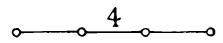
\includegraphics[keepaspectratio]{images/part002_520d8dd1.jpg}}

\begin{enumerate}
\def\labelenumi{(\roman{enumi})}
\setcounter{enumi}{1}
\tightlist
\item
  若边 \(\{1,2\}\) 的阶为 5，则图是下列图之一：
\end{enumerate}

\pandocbounded{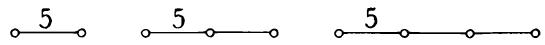
\includegraphics[keepaspectratio]{images/part002_9200390b.jpg}}

由引理 4，可设 \(l > 2\)。假设 \(\{i, i + 1\}\) 的阶为 \(\geqslant 4\)，其中 \(1 \leqslant i \leqslant l - 1\)。置

\(x = e_{1} + 2e_{2} + \dots + ie_{i}, y = e_{l} + 2e_{l - 1} + \dots + (l - i)e_{i + 1},\) 且 \(j = l - i\) .

根据引理 8，\(\| x\|^2 = \frac{1}{2} i(i + 1),\| y\|^2 = \frac{1}{2} j(j + 1)\)。另一方面，\((x|y) = ij(e_i|e_{i + 1}) = -ij\cos \frac{\pi}{m}\)，其中 \(m = 4\) 或 5（引理 4）。现在

\[
(x | y) ^ {2} <   \left\| x \right\| ^ {2} \| y \| ^ {2}.
\]

这给出

\[
\frac {1}{4} i j (i + 1) (j + 1) > i ^ {2} j ^ {2} \cos^ {2} \frac {\pi}{m}
\]

所以

\[
(i + 1) (j + 1) > 4 i j \cos^ {2} \frac {\pi}{m} \geqslant 2 i j.
\]

首先得到 \(ij - i - j - 1 < 0\)，或 \((i - 1)(j - 1) < 2\)。若

\[
1 <   i <   l - 1,
\]

则 \(1 < j < l - 1\)，所以 \(i = j = 2\)，从而 \({}^1\)

\[
9 > 16 \cos^ {2} {\frac {\pi}{m}}, \text {thus} \cos^ {2} {\frac {\pi}{m}} <   \cos^ {2} {\frac {\pi}{5}}
\]

从而 \(m = 4\)。这证明了 (i)。若 \(i = 1\) 且 \(m = 5\)，则 \(2j + 2 > 4j\frac{3 + \sqrt{5}}{8}\)，或 \(j\frac{\sqrt{5} - 1}{2} < 2\)，\(j < \sqrt{5} + 1 < 4\)，所以 \(l = j + 1 \leqslant 4\)。这证明了 (ii)。

引理 10. 若 X 有一个分叉点 i，则完全子图 \(X - \{i\}\) 是三条链的并；若 p - 1、q - 1、r - 1 是这些链的长度，则三元组 \(\{p, q, r\}\) 在置换意义下等于下列三元组之一：\(\{1, 2, 2\}\)、\(\{1, 2, 3\}\)、\(\{1, 2, 4\}\)、\(\{1, 1, m\}\)（某个 \(m \geqslant 1\)）。

顶点 \(i\) 属于 3 条边（引理 2），且没有其他分叉点（引理 7），所以完全子图 \(\mathrm{X} - \{i\}\) 是 3 条链 \(\mathrm{X}_1\)、\(\mathrm{X}_2\)、\(\mathrm{X}_3\) 的并，其中每条链都有一个与 \(i\) 在 \(\mathrm{X}\) 中相连的端点。设 \(\{i_1, i_2\}\)、\(\{i_2, i_3\}, \ldots, \{i_{p-1}, i_p\}\) 是 \(\mathrm{X}_1\) 的边，\(\{j_1, j_2\}\)、\(\{j_2, j_3\}, \ldots, \{j_{q-1}, j_q\}\) 是 \(\mathrm{X}_2\) 的边，\(\{k_1, k_2\}\)、\(\{k_2, k_3\}, \ldots, \{k_{r-1}, k_r\}\) 是 \(\mathrm{X}_3\) 的边，其中 \(i_1, j_1, k_1\) 与 \(i\) 在 \(\mathrm{X}\) 中相连。可设 \(p \geqslant q \geqslant r \geqslant 1\)。置

\[
\begin{array}{l} x = e _ {i _ {p}} + 2 e _ {i _ {p - 1}} + \dots + p e _ {i _ {1}} \\ y = e _ {j _ {q}} + 2 e _ {j _ {q - 1}} + \dots + q e _ {j _ {1}} \\ z = e _ {k _ {r}} + 2 e _ {k _ {r - 1}} + \dots + r e _ {k _ {1}}. \end{array}
\]

由于 X 的所有边的阶都是 3（引理 7），由引理 8 得 \(\| x\|^2 = \frac{1}{2} p(p + 1)\)、\(\| y\|^2 = \frac{1}{2} q(q + 1)\)、\(\| z\|^2 = \frac{1}{2} r(r + 1)\)。另一方面，\(e_i\) 与 \(e_{i_2}, e_{i_3}, \ldots, e_{i_p}\) 正交，故 \((e_i|x) = p(e_i|e_{i_1}) = -\frac{1}{2} p\)；同理 \((e_i|y) = -\frac{1}{2} q\)、\((e_i|z) = -\frac{1}{2} r\)。单位向量 \(\| x\|^ {-1}x\)、\(\| y\|^ {-1}y\)、\(\| z\|^ {-1}z\) 两两正交，且 \(e_i\) 不属于它们生成的子空间 F；从 \(e_i\) 到 F 的距离的平方为

\[
\begin{array}{r l} 1 - (e _ {i} | \frac {x}{\| x \|}) ^ {2} - (e _ {i} | \frac {y}{\| y \|}) ^ {2} - (e _ {i} | \frac {z}{\| z \|}) ^ {2} \\ & = 1 - \frac {1}{2} \frac {p}{p + 1} - \frac {1}{2} \frac {q}{q + 1} - \frac {1}{2} \frac {r}{r + 1} \\ & = 1 - \frac {1}{2} + \frac {1}{2} \frac {1}{p + 1} - \frac {1}{2} + \frac {1}{2} \frac {1}{q + 1} - \frac {1}{2} + \frac {1}{2} \frac {1}{r + 1}. \end{array}
\]

由于此量为 \(>0\)，有

\[
(p + 1) ^ {- 1} + (q + 1) ^ {- 1} + (r + 1) ^ {- 1} > 1.\tag{4}
\]

因此 \(3(r + 1)^{-1} > 1\)，所以 \(r < 2\)，最后 \(r = 1\)。于是由 (4) 得

\[
(p + 1) ^ {- 1} + (q + 1) ^ {- 1} > \frac {1}{2}\tag{5}
\]

故 \(2(q + 1)^{-1} > \frac{1}{2}\)，所以 \(q \leqslant 2\)。最后，若 \(q = 2\)，由 (5) 得

\[
(p + 1) ^ {- 1} > \frac {1}{6}. \quad \text { hence } p \leqslant 4.
\]

定理 1. 任一不可约有限 Coxeter 系统 (W.S) 的图同构于下列图之一：

\pandocbounded{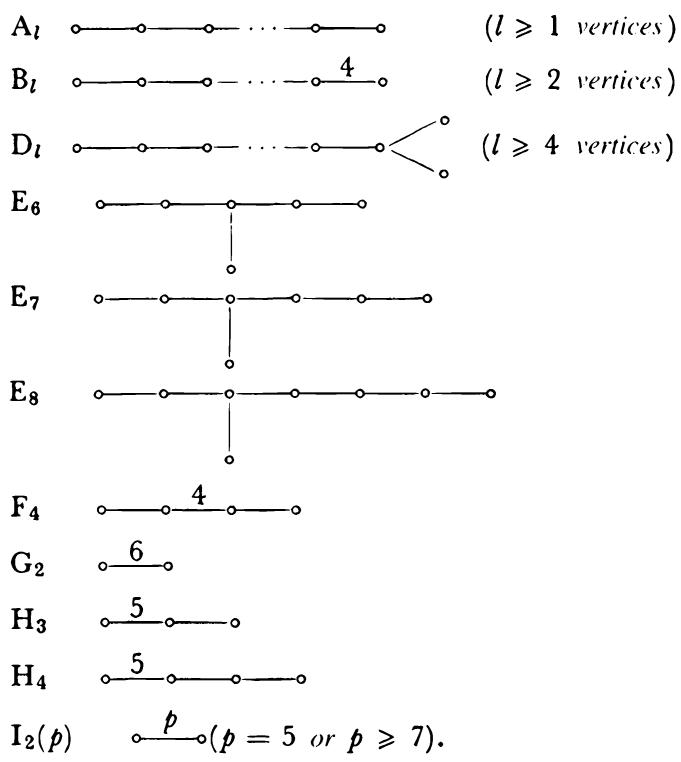
\includegraphics[keepaspectratio]{images/part002_677d99d4.jpg}}

这些图中任意两个都不同构。

事实上，设 \(\mathrm{W} = (m_{ij})\) 是 (W,S) 的 Coxeter 矩阵，且 \(l = \operatorname{Card}(S)\)。若某个 \(m_{ij}\) 为 \(\geqslant 6\)，则 l = 2（引理 4），且 (W,S) 的 Coxeter 图是 \(G_{2}\) 型或 \(I_{2}(p)\) 型，其中 \(p \geqslant 7\)。现在假设所有 \(m_{ij} \leqslant 5\)。

\begin{enumerate}
\def\labelenumi{\alph{enumi})}
\item
  若 \(m_{ij}\) 不全都等于 3，则 (W.S) 的图 X 是一条链，且恰有一个 \(m_{ij}\) 等于 4 或 5（引理 7）。若某个 \(m_{ij}\) 等于 5，则引理 9 表明我们得到 \(H_{3}\)、\(H_{4}\) 或 \(I_{2}(5)\) 型之一。若某个 \(m_{ij}\) 等于 4，则引理 9 表明我们得到 \(B_{l}\) 或 \(F_{4}\) 型之一。
\item
  现在假设所有 \(m_{ij}\) 都等于 3。若 X 是一条链，则 Coxeter 图是 \(A_{l}\) 型。否则，引理 10 表明它是 \(E_{6}\)、\(E_{7}\)、\(E_{8}\) 或 \(D_{l}\) 型。
\end{enumerate}

显然，所列 Coxeter 图中任意两个都不同构。

反之：

定理 2. 定理 1 中由 Coxeter 图 \(\mathbf{A}_l, \mathbf{B}_l, \ldots, \mathbf{I}_2(p)\) 定义的 Coxeter 群是有限的。

对于 \(I_{2}(p)\) 这显然成立，因为相应的群是阶为 2p 的二面体群（第四章第 1 节第 9 号）。对于 \(H_{4}\)，相应的二次型

为

\[
\begin{array}{r l} & \xi_ {1} ^ {2} + \xi_ {2} ^ {2} + \xi_ {3} ^ {2} + \xi_ {4} ^ {2} - \xi_ {1} \xi_ {2} - \xi_ {2} \xi_ {3} - 2 (\cos \frac {\pi}{5}) \xi_ {3} \xi_ {4} \\ & = \xi_ {1} ^ {2} + \xi_ {2} ^ {2} + \xi_ {3} ^ {2} + \xi_ {4} ^ {2} - \xi_ {1} \xi_ {2} - \xi_ {2} \xi_ {3} - \frac {1 + \sqrt {5}}{2} \xi_ {3} \xi_ {4} \\ & = (\xi_ {2} - \frac {\xi_ {1} + \xi_ {3}}{2}) ^ {2} + (\xi_ {4} - \frac {1 + \sqrt {5}}{4} \xi_ {3}) ^ {2} + \frac {3}{4} (\xi_ {1} - \frac {1}{3} \xi_ {3}) ^ {2} + \frac {7 - 3 \sqrt {5}}{24} \xi_ {3} ^ {2}. \end{array}
\]

由于 \(7 - 3\sqrt{5}\) 为 \textgreater0，此形式正且非退化，故相应的 Coxeter 群是有限的。\(H_{3}\) 所对应的情形也如此，因为它同构于前一个群的子群（第四章第 1 节第 8 号）。

对于 \(A_{l}\)、\(B_{l}, \ldots, G_{2}\) 型，我们将在第 5 至 13 号中构造以相应群为韦伊群的根系。我们将看到，这些群不仅有限，而且是晶体群（第 2 节，第 5 号）。

\subsection{Dynkin 图}

依照通常的语言滥用，我们称具有以下性质的一对 \((\Gamma, f)\) 为赋范图：

\begin{enumerate}
\def\labelenumi{\arabic{enumi})}
\item
  \(\Gamma\) 是一个图（称为 \((\Gamma, f)\) 的底图）。
\item
  若 E 表示有序对 \((i,j)\) 所成的集合，其中 \(\{i,j\}\) 是 \(\Gamma\) 的一条边，则 f 是从 E 到 R 的映射，并且有 \(f(i,j)f(j,i)=1\)（对所有 \((i,j)\in\mathbf{E}\)）。
\end{enumerate}

赋范图的同构概念是显然的。

设 R 是实向量空间 V 中的一个约化根系。我们将与之关联一个赋范图 \((X, f)\)，称为 R 的 Dynkin 图。X 的顶点将是 W(R) 在 \(\{B\} \times B\) 的并集（其中 B 为 R 的基集）中的轨道集 I 的元素。若 \(N = (n_{ij})_{i,j \in I}\)（分别为 \(M = (m_{ij})_{i,j \in I}\)）是 R 的典范 Cartan 矩阵（分别为 Coxeter 矩阵）（\(\S\) 1，第 5 号，备注 7），则 X 的两个顶点 i 和 j 相连，当且仅当 \(n_{ij} \neq 0\)，并置

\[
f (i, j) = \frac {n _ {i j}}{n _ {j i}}.
\]

由于 \(n_{ij} = 0\) 蕴含 \(n_{ji} = 0\)，这定义了一个赋范图 (X. f)。

设 \((x|y)\) 是 V 上在 W(R) 下不变的标量积，令 \(B = (\alpha_i)_{i \in I}\) 为 R 的一组按典范方式编号的基。第 1 节第 1 号的公式 (7) 和 (9) 表明，图 X 的顶点 i 和 j 相连，当且仅当

\[
(\alpha_ {i} | \alpha_ {j}) \neq 0
\]

并且

\[
f (i, j) = \frac {\left(\alpha_ {j} \mid \alpha_ {i}\right)}{\left(\alpha_ {j} \mid \alpha_ {j}\right)}.
\]

根据第 1 节第 3 号和第 5 号的结果，除交换 \(i\) 和 \(j\) 外，只有以下可能性：

\begin{enumerate}
\def\labelenumi{\arabic{enumi})}
\item
  \(i\) 和 \(j\) 不相连；\(n_{ij} = n_{ji} = 0\)；\(m_{ij} = 2\)；
\item
  \(f(i,j) = f(j,i) = 1; n_{ij} = n_{ji} = -1; m_{ij} = 3;\)
\item
  \(f(i,j) = 2\)，\(f(j,i) = 1/2\)；\(n_{ij} = -2\)。\(n_{ji} = -1\)；\(m_{ij} = 4\)；
\end{enumerate}

\[
f (i, j) = 3, f (j, i) = 1 / 3: n _ {i j} = - 3, n _ {j i} = - 1; m _ {i j} = 6.
\]

由此可见，Dynkin 图 R 确定 R 的 Cartan 矩阵和 Coxeter 矩阵，因而将 R 确定到同构为止。更精确地说，第 1 节第 5 号命题 15 的推论蕴含以下结果：

命题 1. 设 \(R_{1}\) 和 \(R_{2}\) 是向量空间 \(V_{1}\) 和 \(V_{2}\) 中的两个约化根系。设 \(B_{1} = (\alpha_{i})_{i \in I_{1}}\) 和 \(B_{2} = (\alpha_{i})_{i \in I_{2}}\) 分别为 \(R_{1}\) 和 \(R_{2}\) 的按典范方式编号的基。设 \(\lambda\) 是从 \(R_{1}\) 的 Dynkin 图到 \(R_{2}\) 的 Dynkin 图的同构。则存在唯一的从 \(V_{1}\) 到 \(V_{2}\) 的同构，将 \(R_{1}\) 变为 \(R_{2}\)，并且将 \(\alpha_{i}\) 变为 \(\alpha_{\lambda(i)}\)（对所有 \(i \in I_{1}\)）。

显然，R 的一个自同构定义 R 的 Dynkin 图的一个自同构，从而定义从群 A(R) 到 R 的 Dynkin 图自同构群的同态 \(\varphi\)。

推论。同态 \(\varphi\) 通过取商定义了从群 A(R)/W(R) 到 R 的 Dynkin 图自同构群的一个同构。

显然，\(\varphi(g) = \operatorname{Id}\)（对所有 \(g \in W(R)\)）。另一方面，命题 1 表明，存在一个同构 \(\psi\)，它从 \(R\) 的 Dynkin 图同构群映到 \(E\)，而 \(A(R)\) 中固定给定基 \(B\)（属于 \(R\)）的元素组成此子群，并且满足 \(\varphi \circ \psi = \operatorname{Id}\)。由于 \(A(R)\) 是 \(E\) 与 \(W(R)\) 的半直积（第 1 节，第 5 号，命题 16），推论得证。

实际上，Dynkin 图 \((X, f)\) 用由节点和边组成的图表示如下。节点对应于 X 的顶点；在上述情形 1）、2）、3）和 4）中，分别用 0、1、2 或 3 条边连接对应于两个不同顶点 i 和 j 的两个节点（除交换 i 和 j 外）。此外，在情形 3）和 4）中，即当 \(f(i, j) > 1\)，或根 \(\alpha_{1}\) 与 \(\alpha_{j}\) 不正交且长度不同时，在连接对应于 i 和 j 的节点的双边或三边上放置不等号 \textgreater{}，方向指向对应于 j 的节点（即较短的根）：

\[
\underset {i} {\longrightarrow} \underset {j} {\longrightarrow} \quad (\text { for   } f (i, j) = 2), \quad \underset {i} {\longrightarrow} \underset {j} {\longrightarrow} \quad (\text { for   } f (i, j) = 3).
\]

显然，可以从此图恢复 Dynkin 图 \((X, f)\)。

注意，与 W(R) 的 Coxeter 图对应的图可以从与 R 的 Dynkin 图对应的图得到：保留节点和单边，并将双边（分别为三边）替换为上方标有数字 4（分别为 6）的边。反过来，给定 W(R) 的 Coxeter 图，可以使用此过程的逆过程恢复与 R 的 Dynkin 图对应的图，但双边或三边上的不等号除外。因此定理 1 立即给出可能的 Dynkin 图列表。更精确地说：

定理 3. 若 R 是不可约约化根系，则其 Dynkin 图同构于以下图示中的某一个图：

\pandocbounded{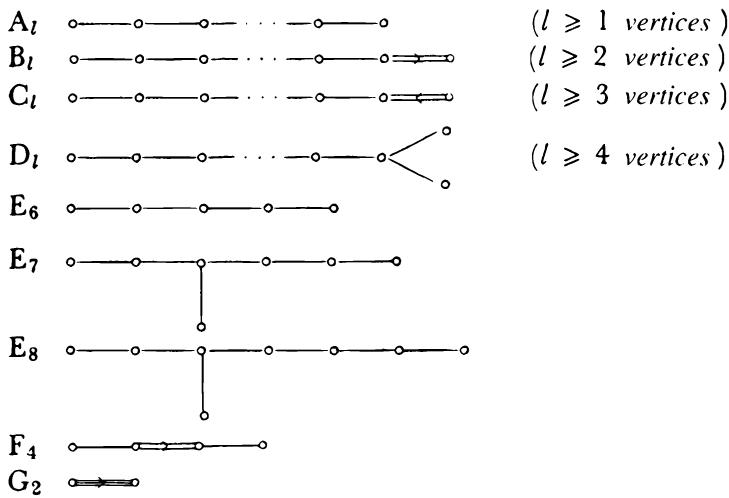
\includegraphics[keepaspectratio]{images/part002_c37a5a77.jpg}}

这些图中任意两个都不同构，并且存在不可约约化根系，使每一个图（在同构意义下）都成为其 Dynkin 图。

第一个断言立即由定理 1、上述备注、图 \(H_{3}\)、\(H_{4}\) 和 \(I_{2}(p)\) 的 Coxeter 群（当 p = 5 及 \(p \geqslant 7\) 时）不是晶体群这一事实，以及与 Coxeter 图 \(F_{4}\)（分别为 \(G_{2}\)）对应的 Dynkin 图的双边（分别为三边）的两种可能不等号给出同构 Dynkin 图这一事实得到。第二个断言是显然的，第三个断言将由对每一种类型明确构造一个不可约约化根系而得出；这一构造将在第 5 至 13 号中进行。

备注。1）图 \(A_{1}\) 退化为一个节点；也记为 \(B_{1}\) 或 \(C_{1}\)。图 \(B_{2}\) 也记为 \(C_{2}\)。图 \(A_{3}\) 也记为 \(D_{3}\)。最后，\(D_{2}\) 表示由两个不相连节点组成的图。（这些约定源于相应根系的性质，参见第 5 至 8 号。）

\begin{enumerate}
\def\labelenumi{\arabic{enumi})}
\setcounter{enumi}{1}
\tightlist
\item
  若 \((X, f)\) 是约化根系 R 的 Dynkin 图，则对偶根系的 Dynkin 图可与 \((X, f^{-1})\) 认同。换言之，与 \(R^{\prime}\) 的 Dynkin 图对应的图可以从与 R 的 Dynkin 图对应的图得到，只需反转不等号。若 R 不可约，则可见 R 与 \(R^{\prime}\) 同构，除非 R 是 \(B_{l}\) 型或 \(C_{l}\) 型；在这两种情形下，\(R^{\prime}\) 分别是 \(C_{l}\) 型或 \(B_{l}\) 型。
\end{enumerate}

\subsection{仿射韦伊群与完备 Dynkin 图}

设 R 是不可约约化根系，\((\mathbf{X}, f)\) 是其 Dynkin 图。我们将定义另一个赋范图 \((\tilde{\mathbf{X}}, \tilde{f})\)，称为 R 的完备 Dynkin 图。\(\tilde{I}\) 是 \(\tilde{X}\) 的顶点集，由 X 的顶点集 I 和一个记为 0 且不属于 I 的顶点组成。为定义 \(\tilde{f}\)，选取 R 的一组基 \(B = (\alpha_{i})_{i \in I}\) 以及在 W(R) 下不变的标量积 \((x|y)\)。令 \(\alpha_{0}\) 为相对于 B 所定义的序的最高根的负根。两个不同顶点 \(i, j \in \tilde{I}\) 相连，当且仅当 \((\alpha_{i}|\alpha_{j}) \neq 0\)，并置

\[
\tilde {f} (i, j) = \frac {\left(\alpha_ {i} \mid \alpha_ {i}\right)}{\left(\alpha_ {j} \mid \alpha_ {j}\right)}.
\]

立即可见，这样定义的图 \(\tilde{X}\) 和映射 \(\tilde{f}\) 不依赖于 B 或标量积的选择。

若秩 \(l\) 的 \(R\) 等于 1，则 \(I = \{i\}\) 且 \(\alpha_0 = -\alpha_1\)；故 \(\tilde{f}(0, i) = 1\)。若 \(l \geqslant 2\)，\(\alpha_0\) 不与任何 \(\alpha_i\) 成比例，且 \((\alpha_0|\alpha_i)\) \(\leqslant 0\)（第 1 节，第 8 号，命题 25）。对于任意一对不同元素 \((i,j)\)（属于 \(\tilde{I}\)），唯一可能性就是前一号中标为 1）、2）、3）、4）的那些可能性（例如置 \(n_{0i} = n(\alpha_0, \alpha_i)\)，\(m_{0i} = \text{阶 } s_{\alpha_0}s_{\alpha_i}\)，其中 \(i \in I\)）。

在 \(l \geqslant 2\) 的情形，完备 Dynkin 图用与前一号相同约定的图表示，有时用虚线表示连接顶点 0 与其他顶点的边。注意，若这种边上存在不等号 \textgreater{}，它总是指向异于 0 的顶点，因为 \(\alpha_{0}\) 是最长根（\(\S\) 1，第 8 号，命题 25）。图 \((\mathbf{X}, f)\) 是从 \((\tilde{\mathbf{X}}, f)\) 删除顶点 0 后得到的子图。

A(R) 在 (X. f) 上的作用延拓为 \((\tilde{\mathbf{X}}.\tilde{f})\) 上的作用，并固定 0；而 W(R) 在 \((\tilde{\mathbf{X}}.\tilde{f})\) 上平凡作用。

我们沿用第 2 节的记号。第 2 节第 2 号的命题 5，连同第五章第 3 节第 2 号的定理 1，表明，仿射韦伊群的 Coxeter 图 \(\Sigma\) 与 \(W_{a}(R)\) 相关；它可以从 \((\tilde{X},\tilde{f})\) 按照由 \(W(R)\) 从 \((X,f)\) 得到其 Coxeter 图的相同规则得到。另一方面，令 G 为 \(W_{a}(R)\) 的正规化子（第 2 节，第 3 号）。对每个 \(g\in G\)，都有一个自同构 \(\varphi(g)\) 作用于 \(\Sigma\)，且 \(\varphi(g)=\mathrm{Id}\)（若 \(g\in W_{a}(R)\)）。反过来，给定 \(\lambda\)，它是 \(\Sigma\) 的一个自同构；根据第五章第 4 节第 9 号的命题 11，存在唯一元素 \(g=\psi(\lambda)\)，保持给定小室 C，并满足 \(\varphi(g)=\lambda\)。由于 G 是保持 C 的元素所成的子群 \(G_{C}\) 与 \(W_{a}(R)\) 的半直积（第 2 节，第 3 号），故 \(\varphi\) 通过取商定义了从 \(G/W_{a}\)（或从 \(G_{C}\)）到 \(\operatorname{Aut}(\Sigma)\) 的同构。立即可见，这个同构与从 A(R)/W(R) 到 G/ \(W_{a}\) 的典范映射的复合，恰好是从 A(R)/W(R) 到 \(\operatorname{Aut}(\Sigma)\) 的同态；这个同态由上面定义的从 A(R)/W(R) 到 \(\operatorname{Aut}(\tilde{X},\tilde{f})\) 的同态所诱导。根据第 2 节第 3 号，群 \(\operatorname{Aut}(\Sigma)\) 同构于

\(A(R)/W(R)\) 与 \(P(R')/Q(R')\) 的半直积，而 \(P(R')/Q(R')\) 同构于群 \(I_{C'} = G_{C'} \cap W_{a}'\)（记号同第 2 节第 3 号）：\(\text{Aut}(\Sigma)\) 中与 \(\gamma_{i}\)（\(I_{C}\) 中的元素）相对应的元素，将顶点 0 变为 \(\Sigma\) 的顶点 i。

备注。可以证明，典范映射

\[
\operatorname{Aut} (\tilde {X}, \tilde {f}) \rightarrow \operatorname{Aut} (\Sigma)
\]

是一个同构。

定理 4. 设 (W.S) 是 S 有限的不可约 Coxeter 系统。关联的二次型（第五章第 4 节第 1 号）正且退化，当且仅当 (W.S) 的 Coxeter 图同构于下列图之一：

\pandocbounded{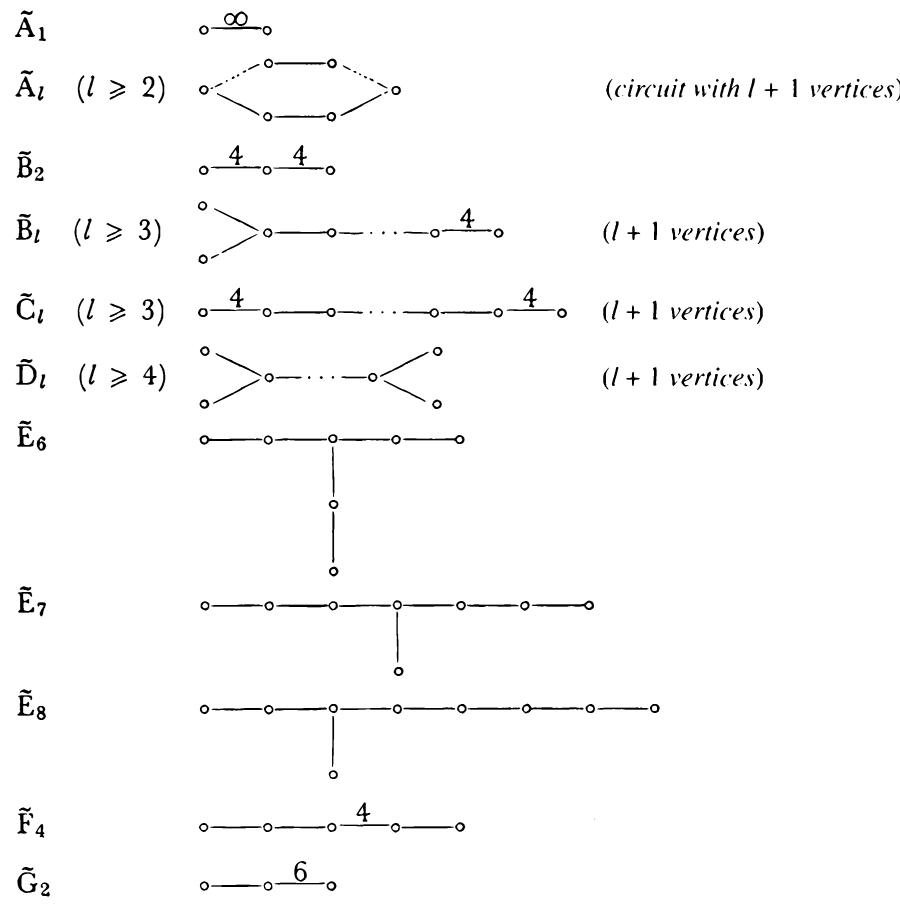
\includegraphics[keepaspectratio]{images/part002_b5f8d83f.jpg}}

这些 Coxeter 图中任意两个都不同构。

根据第五章第 4 节第 9 号以及第 2 节第 5 号的命题 8，二次型正且退化的 Coxeter 系统正是对应于不可约约化根系的仿射韦伊群的那些系统。因此，定理由下面第 5 至 13 号中对完备 Dynkin 图的确定得出。

\subsection{根系构造的预备知识}

设 V 是一个维数 \(l \geqslant 1\) 的实向量空间，并配备标量积 \((x|y)\)。设 L 是 V 的离散子群，A 是一个有限的数集，且其中每个数为 \textgreater0；R 是由这样的元素组成的集合：\(\alpha \in L\)，且 \((\alpha|\alpha) \in \Lambda\)。假设 R 生成 V，并且对于 R 中任意一对点 \((\alpha,\beta)\)，数 \(2\frac{(\alpha|\beta)}{(\alpha|\alpha)}\) 是整数。则 R 是 V 中的根系。事实上，R 显然满足 \((RS_{I})\)。令 \(\alpha \in R\)：令 \(s_{\alpha}\) 为正交反射 \(x \mapsto x - 2\frac{(x|\alpha)}{(\alpha|\alpha)}\alpha\)；于是若 \(\beta \in R\)，有 \(2\frac{(\beta|\alpha)}{(\alpha|\alpha)} \in Z\)，故 \(s_{\alpha}(\beta) \in L\)，且 \(\|s_{\alpha}(\beta)\| = \| \beta \|\)，所以 \(s_{\alpha}(\beta) \in R\)；因此 R 满足 \((RS_{II})\) 和 \((RS_{III})\)，并且若 A 不含形如 \(\lambda\) 和 \(4\lambda\) 的两个数，则 R 是约化的。

现在令 V 为 \(E = R^{n}\) 的一个子空间。令 \((\varepsilon_{1}, \ldots, \varepsilon_{n})\) 为 E 的典范基；在 E 上取使此基成为标准正交基的标量积，并借助此标量积将 \(E^{*}\) 与 E（分别将 \(V^{*}\) 与 V）认同。定义 E 的子群 \(L_{0}, L_{1}, L_{2}, L_{3}\) 如下：

\begin{enumerate}
\def\labelenumi{\arabic{enumi})}
\item
  \(L_{0}\) 是以 \((\varepsilon_{i})\) 为基的 Z-模。我们有 \((\alpha|\beta)\in\mathbf{Z}\)，其中 \(\alpha,\beta\in L_{0}\)。满足条件 \(\alpha\in L_{0}\) 且 \((\alpha|\alpha)=1\) 的向量是 \(\pm\varepsilon_{i}\;(1\leqslant i\leqslant n)\)；满足 \((\alpha|\alpha)=2\) 的向量是 \(\pm\varepsilon_{i}\pm\varepsilon_{j}\)，其中 i\textless j（\(\pm\) 中的两个符号，在 \(\pm\varepsilon_{i}\pm\varepsilon_{j}\) 中彼此独立选取；本节其余部分均采用类似约定）。
\item
  \(L_{1}\) 是 \(L_{0}\) 的 Z-子模，由 \(x = \sum_{i=1}^{n} \xi_{i} \varepsilon_{i} \in L_{0}\) 组成，其中 \(\sum_{i=1}^{n} \xi_{i}\) 为偶数；由于 \(\xi_{i}\) 与 \(\xi_{i}^{2}\) 具有相同的奇偶性，这等价于要求 \((x|x)\) 为偶数。令 \(L_{1}^{\prime}\) 为 \(L_{1}\) 的子模，由 \(\varepsilon_{i} \pm \varepsilon_{j}\) 生成；我们有 \(\sum_{i=1}^{n} \xi_{i} \varepsilon_{i} \equiv (\sum_{i=1}^{n} \xi_{i}) \varepsilon_{n} \pmod{L_{1}^{\prime}}\)，且由于 \(2\varepsilon_{n} = (\varepsilon_{1} + \varepsilon_{n}) - (\varepsilon_{1} - \varepsilon_{n}) \in L_{1}^{\prime}\)，可知 \(L_{1}^{\prime} = L_{1}\)。由于 \(L_{0}\) 由 \(L_{1}\) 和 \(\varepsilon_{1}, L_{0}/L_{1}\) 生成，后者同构于 Z/2Z。
\item
  \(\mathrm{L}_2 = \mathrm{L}_0 + \mathbf{Z}\left(\frac{1}{2} \sum_{i=1}^{n} \varepsilon_i\right)\)。显然，元素 \(x = \sum_{i=1}^{n} \xi_i \varepsilon_i\) 属于 \(\mathrm{V}\)，它属于 \(\mathrm{L}_2\) 当且仅当
\end{enumerate}

\[
2 \xi_ {i} \in \mathbf {Z}, \quad \xi_ {i} - \xi_ {j} \in \mathbf {Z} \text {   for   all   } i \text {   and   } j.\tag{6}
\]

由于 \((\varepsilon_k|_{\frac{1}{2}}\sum_{i=1}^{n}\varepsilon_i) = \frac{1}{2}\) 对所有 \(k\) 成立，且 \(\| \frac{1}{2}\sum_{i=1}^{n}\varepsilon_i\|^2 = \frac{n}{4}\)，有 \((\alpha|\beta) \in \frac{1}{2}\mathbf{Z}\) 对于 \(\alpha, \beta \in L_2\) 成立，其中 \(n\) 为偶数。群 \(L_2 / L_0\) 同构于 \(\mathbf{Z}/2\mathbf{Z}\)。

\begin{enumerate}
\def\labelenumi{\arabic{enumi})}
\setcounter{enumi}{3}
\tightlist
\item
  \(L_{3} = L_{1} + \mathbf{Z}\left(\frac{1}{2} \sum_{i=1}^{n} \varepsilon_{i}\right)\)。若 n 是 4 的倍数，则 \(L_{3}\) 是由 \(\sum_{i=1}^{n} \xi_{i} \varepsilon_{i}\) 组成的集合，这些元素满足 (6) 以及条件 \(\sum_{i=1}^{n} \xi_{i} \in 2\mathbf{Z}\)；在此情形，\((\alpha | \beta) \in \mathbf{Z}\) 对所有 \(\alpha, \beta \in L_{3}\) 成立。
\end{enumerate}

立即可见，与 \(L_{0}\)（分别为 \(L_{1}, L_{2}\)）关联的 E 的子群是 \(L_{0}\)（分别为 \(L_{2}, L_{1}\)）。与 \(L_{3}\) 关联的 E 的子群是

\[
x = \sum_ {i = 1} ^ {n} \xi_ {i} \varepsilon_ {i} \in L _ {2}
\]

满足 \((x|\frac{1}{2}\sum_{i = 1}^{n}\varepsilon_i)\in \mathbf{Z}\)，即满足 \(\sum_{i = 1}^{n}\xi_{i}\in 2\mathbf{Z}\)；因此若 \(n\equiv 0\)（模 4），这个关联子群就是 \(\mathrm{L}_3\)。

阿贝尔群 \(\mathrm{L}_2 / \mathrm{L}_1\) 的阶为 4，因而同构于 \(\mathbf{Z} / 4\mathbf{Z}\) 或 \(\mathbf{Z} / 2\mathbf{Z} \times \mathbf{Z} / 2\mathbf{Z}\)（《代数》第七章第 4 节第 6 号定理 3）。若 \(n\) 为奇数，

\[
p (\frac {1}{2} \sum_ {i = 1} ^ {n} \varepsilon_ {i}) \in \mathrm{L} _ {1} \Leftrightarrow p \equiv 0 (\mathrm{mod.} 4)
\]

所以 \(\mathrm{L}_2 / \mathrm{L}_1\) 是 4 阶循环群。若 \(n\) 为偶数，

\[
p (\frac {1}{2} \sum_ {i = 1} ^ {n} \varepsilon_ {i}) \in \mathrm{L} _ {1} \Leftrightarrow p \equiv 0 (\mathrm{mod.} 2)
\]

所以 \(L_{2}/L_{1}\) 含有两个不同的 2 阶元素，并同构于 \(Z/2Z \times Z/2Z\)。

在下面九个号以及各图版中，我们将一直使用这些记号。对于定理 3 中的每一种 Dynkin 图，我们将明确描述：

\begin{enumerate}
\def\labelenumi{(\Roman{enumi})}
\item
  一个根系 R 及其根的数目。
\item
  R 的一组基 B 及相应的正根。基 B 将用整数 \(1,\ldots,l\) 编号。
\item
  Coxeter 数 \(h\)（第 1 节，第 11 号）。
\item
  最高根 \(\tilde{\alpha}\)（相对于 B 所定义的序）及完备 Dynkin 图（第 3 号）。我们将在每个顶点旁标出 B 中对应的根。
\item
  对偶根系 \(\mathbb{R}^{\prime}\)、典范双线性形式以及常数 \(\gamma(\mathbb{R})\)（第 1 节，第 12 号）。
\item
  相对于 B 的基本权（第 1 节，第 10 号）。
\item
  正根之和。
\item
  群 \(P(R), Q(R), P(R)/Q(R)\) 以及连接指标（第 1 节，第 9 号）。
\item
  \(\mathrm{W}(\mathrm{R})\) 的指数（第五章第 6 节第 2 号定义 2）。在 \(\mathbf{A}_l, \mathbf{B}_l, \mathbf{C}_l\) 和 \(\mathbf{D}_l\) 的情形，我们确定其对称不变量。
\item
  W(R) 的阶（以及在某些情形下它的结构）。
\item
  群 \(A(R)/W(R)\)、它在 Dynkin 图上的作用，以及将 B 变为 -B 的元素 \(w_{0}\)（属于 \(W(R)\)）。
\item
  \(\mathrm{P}(\mathrm{R}^{\prime})/\mathrm{Q}(\mathrm{R}^{\prime})\) 在完备 Dynkin 图上的作用，以及 \(\mathrm{A}(\mathrm{R})/\mathrm{W}(\mathrm{R})\) 在 \(\mathrm{P}(\mathrm{R}^{\prime})/\mathrm{Q}(\mathrm{R}^{\prime})\) 上的作用。
\end{enumerate}

对于定理 3 中的每个 Dynkin 图，这些数据将汇集于图版 I 至 IX 中，并按上述统一方式排列。我们还给出：

\begin{enumerate}
\def\labelenumi{(\Roman{enumi})}
\setcounter{enumi}{12}
\tightlist
\item
  Cartan 矩阵，由它按第 2 号所述方式导出 Dynkin 图。
\end{enumerate}

\subsection{\texorpdfstring{\(B_{l}\) 型根系（\(l \geqslant 2\)）}{B\_l 型根系 (l >= 2)}}

\begin{enumerate}
\def\labelenumi{(\Roman{enumi})}
\item
  我们考虑 \(L_{0}\)，它是 V = \(R^{l}\)（第 4 号）中的群。令 R 为由满足 \(\alpha \in L_{0}\) 且 \((\alpha|\alpha) = 1\) 或 \((\alpha|\alpha) = 2\) 的元素所成的集合，换言之，是由向量 \(\pm\varepsilon_{i}\)（\(1 \leqslant i \leqslant l\)）和 \(\pm\varepsilon_{i} \pm \varepsilon_{j}\)（\(1 \leqslant i < j \leqslant l\)）组成的集合。显然，R 生成 V，且 \(2(\alpha|\beta)/(\alpha|\alpha) \in \mathbf{Z}\) 对所有 \(\alpha, \beta \in R\) 成立。因此 R 是 V 中的约化根系（第 4 号）。根的数目为 \(n = 2l + 4\frac{l(l-1)}{2} = 2l^{2}\)。
\item
  置
\end{enumerate}

\[
\alpha_ {1} = \varepsilon_ {1} - \varepsilon_ {2}, \alpha_ {2} = \varepsilon_ {2} - \varepsilon_ {3}, \dots , \alpha_ {l - 1} = \varepsilon_ {l - 1} - \varepsilon_ {l}, \alpha_ {l} = \varepsilon_ {l}.
\]

于是

\[
\begin{array}{c} \varepsilon_ {i} = \alpha_ {i} + \alpha_ {i + 1} + \dots + \alpha_ {l} \quad (1 \leqslant i \leqslant l) \\ \varepsilon_ {i} + \varepsilon_ {j} = (\alpha_ {i} + \alpha_ {i + 1} + \dots + \alpha_ {l}) + (\alpha_ {j} + \alpha_ {j + 1} + \dots + \alpha_ {l}) (1 \leqslant i <   j \leqslant l) \\ \varepsilon_ {i} - \varepsilon_ {j} = \alpha_ {i} + \alpha_ {i + 1} + \dots + \alpha_ {j - 1} \quad (1 \leqslant i <   j \leqslant l). \end{array}
\]

因此 \((\alpha_{1},\alpha_{2},\ldots ,\alpha_{l})\) 是 R 的一组基（第 1 节，第 7 号，命题 20 的推论 3）。此外，\(\| \alpha_{i}\|^{2} = 2\) 对 \(i < l\) 成立，\(\| \alpha_l\| ^2 = 1\)，\((\alpha_i|\alpha_{i + 1}) = -1\) 对 \(1\leqslant i\leqslant l - 1\) 成立，\((\alpha_i|\alpha_j) = 0\) 对 \(j > i + 1\) 成立：因此 R 的 Dynkin 图为 \(\mathbf{B}_l\) 型，这表明 R 不可约。正根是 \(\varepsilon_{i}\) 以及 \(\varepsilon_{i}\pm \varepsilon_{j}\)（\(i < j\)）。

\begin{enumerate}
\def\labelenumi{(\Roman{enumi})}
\setcounter{enumi}{2}
\tightlist
\item
  根据第五章第 6 节第 2 号定理 1 (ii)。
\end{enumerate}

\[
h = n / l = 2 l.
\]

\begin{enumerate}
\def\labelenumi{(\Roman{enumi})}
\setcounter{enumi}{3}
\tightlist
\item
  令 \(\tilde{\alpha} = \varepsilon_{1} + \varepsilon_{2} = \alpha_{1} + 2\alpha_{2} + 2\alpha_{3} + \cdots + 2\alpha_{l}\)，这是一个根。它相对于基 \((\alpha_{i})\) 的坐标之和为 2l - 1 = h - 1。根据第 1 节第 11 号命题 31，\(\tilde{\alpha}\) 是 R 的最高根。有 \((\tilde{\alpha}| \alpha_{i}) = 0\) 对 \(i \neq 2\) 成立，且 \((\tilde{\alpha}| \alpha_{2}) = 1\)。由于 \(\alpha_{2}\) 的长度分别为 1 和 \(\sqrt{2}\)，对应于 l = 2 和 \(l \geqslant 3\)，R 的完备 Dynkin 图如下：
\end{enumerate}

\[
\text { for } l = 2 \quad \alpha_ {2} \alpha_ {1}
\]

\pandocbounded{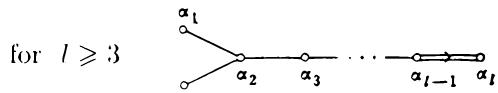
\includegraphics[keepaspectratio]{images/part002_79c781e2.jpg}}

\begin{enumerate}
\def\labelenumi{(\Alph{enumi})}
\setcounter{enumi}{21}
\tightlist
\item
  公式 \(\alpha^{\prime} = \frac{2\alpha}{(\alpha|\alpha)}\) 给出 \(R^{\prime}\) 的向量集：\(\pm 2\varepsilon_{i}\)（\(1 \leqslant i \leqslant l\)）以及 \(\pm \varepsilon_{i} \pm \varepsilon_{j}\)（\(1 \leqslant i < j \leqslant l\)）。\(R^{\prime}\) 的 Dynkin 图按照第 2 号所述过程由 \(R\) 的 Dynkin 图得到，并可见 \(R^{\prime}\) 为 \(C_{l}\) 型。
\end{enumerate}

有 \(4l - 2\) 个根不与 \(\beta = \varepsilon_1\) 正交，即 \(\pm \varepsilon_1\) 以及 \(\pm \varepsilon_1 \pm \varepsilon_j\)（\(2 \leqslant j \leqslant l\)）；对于每个这样的根 \(\alpha\)，\(n(\alpha, \beta) = \pm 2\)。第 1 节第 12 号的公式 (17) 表明，对于 \(\Phi_{\mathrm{R}}\)，\(\beta\) 的长度平方为 \((4l - 2)^{-1}\)；因此 \(\Phi_{\mathrm{R}}(x, y) = (x|y)/(4l - 2)\)。在 \(x = y = \beta\) 的情形应用第 1 节第 12 号的公式 (18)。这给出

\[
2 + \frac {1}{4} (4 l - 4) = \gamma (R) \frac {1}{4 l - 2}
\]

从而 \(\gamma(R) = (l + 1)(4l - 2)\)。

\begin{enumerate}
\def\labelenumi{(\Roman{enumi})}
\setcounter{enumi}{5}
\tightlist
\item
  基本权 \(\omega_{i}\)（\(1 \leqslant i \leqslant l\)）满足 \((\omega_{i}|\alpha_{j}) = \delta_{ij}\)，容易计算，得到
\end{enumerate}

\[
\begin{array}{l} \omega_ {i} = \varepsilon_ {1} + \varepsilon_ {2} + \dots + \varepsilon_ {i} \\ \qquad = \alpha_ {1} + 2 \alpha_ {2} + \dots + (i - 1) \alpha_ {i - 1} + i (\alpha_ {1} + \alpha_ {i + 1} + \dots + \alpha_ {l}) (i <   l) \\ \omega_ {l} = \frac {1}{2} (\varepsilon_ {1} + \varepsilon_ {2} + \dots + \varepsilon_ {l}) = \frac {1}{2} (\alpha_ {1} + 2 \alpha_ {2} + \dots + l \alpha_ {l}). \end{array}
\]

\begin{enumerate}
\def\labelenumi{(\Roman{enumi})}
\setcounter{enumi}{6}
\tightlist
\item
  正根之和为
\end{enumerate}

\[
\begin{array}{l} 2 \rho = (2 l - 1) \varepsilon_ {1} + (2 l - 3) \varepsilon_ {2} + \dots + 3 \varepsilon_ {l - 1} + \varepsilon_ {l} \\ = (2 l - 1) \alpha_ {1} + 2 (2 l - 2) \alpha_ {2} + \dots + i (2 l - i) \alpha_ {i} + \dots + l ^ {2} \alpha_ {l}. \end{array}
\]

\begin{enumerate}
\def\labelenumi{(\Roman{enumi})}
\setcounter{enumi}{7}
\item
  有 \(Q(R) = L_{0}\)（第 4 号），且 \(P(R)\) 由 \(Q(R)\) 和 \(\omega_{l}\) 生成，故等于 \(L_{2}\)（第 4 号）。因此，\(P(R)/Q(R)\) 同构于 Z/2Z，连接指标等于 2。
\item
  以及 (X) 在 \(R^{l}\) 中，正交反射 \(s_{\varepsilon_{i}-\varepsilon_{j}}\)（\(i \neq j\)）交换 \(\varepsilon_{i}\) 和 \(\varepsilon_{j}\)，并在指标 k 异于 i 和 j 时保持 \(\varepsilon_{k}\) 不变。\(s_{\varepsilon_{i}-\varepsilon_{j}}\) 生成一个群 \(G_{1}\)，它同构于对称群 \(S_{l}\)。正交反射 \(s_{\varepsilon_{i}}\) 将 \(\varepsilon_{i}\) 变为 \(-\varepsilon_{i}\)，并在指标 k 异于 i 时保持 \(\varepsilon_{k}\) 不变。\(s_{\varepsilon_{i}}\) 生成一个群 \(G_{2}\)，它同构于 \((\mathbf{Z}/2\mathbf{Z})^{l}\)。韦伊群 W(R) 由 \(G_{1}\) 和 \(G_{2}\) 生成，且 \(G_{2}\) 是 W(R) 的正规子群，所以 W(R) 同构于 \(S_{l}\) 与 \((\mathbf{Z}/2\mathbf{Z})^{l}\) 的半直积。因此它的阶为 \(2^{l}\cdot l!\)。
\end{enumerate}

对称代数 \(\mathbf{S}(\mathbf{R}^{l})\) 可典范地与多项式函数代数 \(\mathrm{P}(\xi_{1},\ldots,\xi_{l})\) 认同，后者定义在 \(R^{l}\) 上。要使这样的多项式在 \(\mathrm{W}(\mathrm{R})\) 下不变，首先必须有

\[
P \left(\xi_ {1}. \xi_ {2}. \dots ., \xi_ {l}\right) = P \left(\pm \xi_ {1}. \pm \xi_ {2}. \dots ., \pm \xi_ {l}\right)
\]

对右端的符号作任意选择均成立，从而

\[
\mathrm{P} \left(\xi_ {1}, \dots , \xi_ {l}\right) = \mathrm{Q} \left(\xi_ {1} ^ {2}, \dots , \xi_ {l} ^ {2}\right)
\]

其中 Q 是多项式，并且 Q 还是对称多项式；这些条件也是充分的。因此（《代数》第五章附录 I），\(\mathbf{S}(\mathbf{R}^{l})^{\mathrm{W}(\mathbb{R})}\) 是由以下 l 个多项式函数生成的代数

\[
t _ {i} = \sum_ {\tau \in \mathfrak {S} _ {l}} \xi_ {\tau (1)} ^ {2} \xi_ {\tau (2)} ^ {2} \dots \xi_ {\tau (l)} ^ {2} \quad (1 \leqslant i \leqslant l).
\]

此外，\(\mathbf{R}\) 上的 \(\mathbf{S}(\mathbf{R}^l)^{\mathrm{W(R)}}\) 的分式域的超越次数为 \(l\)，所以 \(t_i\) 代数独立。由于 \(t_i\) 的次数为 \(2,4,\ldots ,2l\)，我们得到 \(\mathrm{W(R)}\) 的指数（第五章第 6 节第 3 号命题 3）为：

\[
1, 3, 5, \dots , 2 l - 1.
\]

\begin{enumerate}
\def\labelenumi{(\Roman{enumi})}
\setcounter{enumi}{10}
\item
  Dynkin 图的唯一自同构是恒等元。因此，\(A(R) = W(R)\) 且 \(-1 \in W(R)\)。由于 -1 将 B 变为 -B，我们得到 \(w_{0} = -1\)。
\item
  群 \(P(R^{\prime})/Q(R^{\prime})\) 是 \(P(R)/Q(R)\) 的对偶，因而同构于 Z/2Z。其非平凡元置换对应于 \(\alpha_{0}\) 和 \(\alpha_{1}\) 的顶点，并固定其他顶点。
\end{enumerate}

\subsection{\texorpdfstring{\(C_{l}\) 型系统 (\(l \geqslant 2\))}{C\_l 型系统 (l >= 2)}}

\begin{enumerate}
\def\labelenumi{(\Roman{enumi})}
\item
  \(C_{l}\) 型根系的存在已在第 5 号中得到证明，因为我们已经看到，\(B_{l}\) 型系统的逆系统是 \(C_{l}\) 型。因此，一个 \(C_{l}\) 型根系可由在 \(R^{l}\) 中取向量 \(\pm2\varepsilon_{i}\ (1\leqslant i\leqslant l)\) 和 \(\pm\varepsilon_{i}\pm\varepsilon_{j}\ (1\leqslant i<j\leqslant l)\) 得到。根的数目为 \(2l^{2}\)。
\item
  对第 5 号中所考察系统的基应用映射 \(\alpha\mapsto\frac{2\alpha}{(\alpha|\alpha)}\) 所得的像，可以作为 R 的一个基。我们得到：
\end{enumerate}

\[
\alpha_ {1} = \varepsilon_ {1} - \varepsilon_ {2}, \alpha_ {2} = \varepsilon_ {2} - \varepsilon_ {3}, \dots , \alpha_ {l - 1} = \varepsilon_ {l - 1} - \varepsilon_ {l}, \alpha_ {l} = 2 \varepsilon_ {l}.
\]

正根是 \(2\varepsilon_{i}\) 以及 \(\varepsilon_{i} \pm \varepsilon_{j} (i < j)\)。

\begin{enumerate}
\def\labelenumi{(\Roman{enumi})}
\setcounter{enumi}{2}
\item
  Coxeter 数与逆系统的相同：\(h = 2l\)。
\item
  令 \(\tilde{\alpha}=2\varepsilon_{1}=2\alpha_{1}+2\alpha_{2}+\cdots+2\alpha_{l-1}+\alpha_{l}\)，这是一个根。相对于 \((\alpha_{i})\)，它的坐标之和为 2l-1=h-1。因此，\(\tilde{\alpha}\) 是最高根。我们有 \((\tilde{\alpha}|\alpha_{i})=0\)（当 \(i\neq l\) 时），\((\tilde{\alpha}|\alpha_{l})=2\)。从而，扩展 Dynkin 图为
\end{enumerate}

\[
\alpha_ {1} \quad \alpha_ {2} \quad \dots \quad \alpha_ {l - 2} \quad \alpha_ {l - 1} \quad \alpha_ {l}
\]

\begin{enumerate}
\def\labelenumi{(\Alph{enumi})}
\setcounter{enumi}{21}
\tightlist
\item
  我们已经确定了 \(R^{-}\)，它是 \(B_{l}\) 型的。由 § 1 第 12 号的公式 (19) 及第 5 号 (V)，\(2\varepsilon_{i}\) 在 \(\Phi_{R}\) 下的长度平方为
\end{enumerate}

\[
((l + 1) (4 l - 2)) ^ {+ 1} ((4 l - 2) ^ {- 1}) ^ {- 1} = (l + 1) ^ {- 1};
\]

从而，\(\Phi_{\mathrm{R}}(x,y) = (x|y) / 4(l + 1)\)。

我们有 \(\gamma(R) = \gamma(R') = (l + 1)(4l - 2)\)。

\begin{enumerate}
\def\labelenumi{(\Roman{enumi})}
\setcounter{enumi}{5}
\tightlist
\item
  基本权容易求得：
\end{enumerate}

\[
\begin{array}{l} \omega_ {i} = \varepsilon_ {1} + \varepsilon_ {2} + \dots + \varepsilon_ {i} \\ = \alpha_ {1} + 2 \alpha_ {2} + \dots + (i - 1) \alpha_ {i - 1} + i (\alpha_ {i} + \alpha_ {i + 1} + \dots + \frac {1}{2} \alpha_ {l}) (i \leqslant l). \end{array}
\]

\begin{enumerate}
\def\labelenumi{(\Roman{enumi})}
\setcounter{enumi}{6}
\tightlist
\item
  正根之和为
\end{enumerate}

\[
\begin{array}{r l} 2 \rho & = 2 l \varepsilon_ {1} + (2 l - 2) \varepsilon_ {2} + \dots + 4 \varepsilon_ {l - 1} + 2 \varepsilon_ {l} \\ & = 2 l \alpha_ {1} + 2 (2 l - 1) \alpha_ {3} + \dots + i (2 l - i + 1) \alpha_ {i} + \dots \\ & \qquad \dots + (l - 1) (l + 2) \alpha_ {l - 1} + \frac {1}{2} l (l + 1) \alpha_ {l}. \end{array}
\]

\begin{enumerate}
\def\labelenumi{(\Roman{enumi})}
\setcounter{enumi}{7}
\item
  根据第 4 号和第 5 号 (VIII)，\(Q(R) = L_{1}\)，\(P(R) = L_{0}\)；\(P(R)/Q(R)\) 同构于 Z/2Z，连接指标为 2。
\item
  以及 (X) 这些数据只取决于 W(R)，因此与 \(B_{l}\) 型的相同。
\item
  与第 5 号中相同的论证表明 \(A(R) = W(R)\) 且 \(w_0 = -1\)。
\item
  \(\mathrm{P}(\mathrm{R}^{-})/\mathrm{Q}(\mathrm{R}^{-})\) 的唯一非单位元定义了扩展 Dynkin 图的唯一非平凡自同构：它把对应于 \(\alpha_{j}\) 和 \(\alpha_{l-j}\)（\(0 \leqslant j \leqslant l\)）的顶点互换。
\end{enumerate}

\subsection{\texorpdfstring{\(\mathbf{A}_l\) 型系统 (\(l \geqslant 1\))}{A\_l 型系统 (l >= 1)}}

\begin{enumerate}
\def\labelenumi{(\Roman{enumi})}
\tightlist
\item
以及 (II) 设 \(V\) 是 \(E = R^{l + 1}\) 中方程为 \(\sum_{i=1}^{l + 1} \xi_i = 0\) 的超平面。将第 5 号中的 \(l\) 换成 \(l + 1\)，我们得到一个 \(R'\) 的 \(B_{l + 1}\) 型系统，它位于 \(E\) 中，其基为
\end{enumerate}

\[
\alpha_ {1} = \varepsilon_ {1} - \varepsilon_ {2}, \alpha_ {2} = \varepsilon_ {2} - \varepsilon_ {3}, \dots , \alpha_ {l} = \varepsilon_ {l} - \varepsilon_ {l + 1}. \alpha_ {l + 1} = \varepsilon_ {l + 1}.
\]

由于 \(\alpha_{1},\ldots,\alpha_{l}\) 生成 V，\(R=R^{\prime}\cap V\) 是 V 中以 \((\alpha_{1},\ldots,\alpha_{l})\) 为基的根系（§ 1，第 7 号，命题 20 的推论 4）。根据第 5 号中的标量积计算，立即可知 R 是 \(A_{l}\) 型的。R 的元素是 \(\varepsilon_{i}-\varepsilon_{j}\)（\(i\neq j,1\leqslant i\leqslant l+1,1\leqslant j\leqslant l+1\)）。根的数目为 \(n=l(l+1)\)。正根是 \(\varepsilon_{i}-\varepsilon_{j}\)，其中 \(i<j\)。

\begin{enumerate}
\def\labelenumi{(\Roman{enumi})}
\setcounter{enumi}{2}
\item
  我们有 \(h = n / l = l + 1\)。
\item
  令 \(\tilde{\alpha} = \varepsilon_1 - \varepsilon_{l+1} = \alpha_1 + \alpha_2 + \cdots + \alpha_l\)，这是一个根。相对于 \((\alpha_i)\)，它的坐标之和为 \(l = h - 1\)。因此，\(\tilde{\alpha}\) 是最高根。
\end{enumerate}

当 \(l = 1\) 时，\(\tilde{\alpha} = \alpha_{1}\)，所以 \((\tilde{\alpha}|\alpha_{1}) = 2\)；群 \(W_{a}(R)\) 的 Coxeter 图为

当 \(l \geqslant 2\) 时，\((\tilde{\alpha}|\alpha_i) = 0\) 对 \(0 < i < l\) 成立，且 \((\tilde{\alpha}|\alpha_1) = (\tilde{\alpha}|\alpha_l) = 1\)。因此，扩展 Dynkin 图为：

\pandocbounded{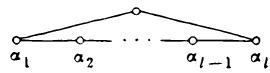
\includegraphics[keepaspectratio]{images/part002_36cfe44b.jpg}}

\begin{enumerate}
\def\labelenumi{(\Alph{enumi})}
\setcounter{enumi}{21}
\tightlist
\item
利用标量积将 V 与其对偶识别，我们有 \(\alpha^{\prime} = \frac{2\alpha}{(\alpha|\alpha)} = \alpha\) 对所有 \(\alpha \in R\) 成立，所以 \(R^{\prime} = R\)。
\end{enumerate}

对于形式 \(\Phi_{\mathbb{R}}\)，根的长度为 \(h^{-1/2} = (l + 1)^{-1/2}\)（§ 1，第 12 号）；因此 \(\Phi_{\mathrm{R}}(x,y) = (x|y)/2(l+1)\)。

我们有 \(\gamma (\mathbb{R}) = (l + 1)^2\)（§ 1，第 12 号，公式 (20)）。

\begin{enumerate}
\def\labelenumi{(\Roman{enumi})}
\setcounter{enumi}{5}
\tightlist
\item
  令 \((\omega_{i})_{1\leqslant i\leqslant l}\) 为基本权族。置
\end{enumerate}

\[
\omega_ {i} = \sum_ {j = 1} ^ {l + 1} \xi_ {i j} \varepsilon_ {j}. \quad \text { with } \xi_ {i j} \in \mathbf {R}.
\]

条件 \((\omega_{i}|\alpha_{j}) = \delta_{ij}\) 和 \(\omega_{i}\in V\) 给出

\[
\xi_ {i i} - \xi_ {i, i + 1} = 1, \quad \xi_ {i j} - \xi_ {i, j + 1} = 0 \text {   for   } j \neq i, \quad \sum_ {j = 1} ^ {l + 1} \xi_ {i j} = 0,
\]

由此容易得到

\[
\begin{array}{r l} \omega_ {i} & = \varepsilon_ {1} + \dots + \varepsilon_ {i} - \frac {i}{l + 1} (\varepsilon_ {1} + \dots + \varepsilon_ {l + 1}) \\ & = \frac {1}{l + 1} ((l - i + 1) (\alpha_ {1} + 2 \alpha_ {2} + \dots + (i - 1) \alpha_ {i - 1}) \\ & \quad + i ((l - i + 1) \alpha_ {i} + (l - i) \alpha_ {i + 1} + \dots + \alpha_ {l})). \end{array}
\]

\begin{enumerate}
\def\labelenumi{(\Roman{enumi})}
\setcounter{enumi}{6}
\tightlist
\item
  正根之和为
\end{enumerate}

\[
\begin{array}{r l} 2 \rho & = l \varepsilon_ {1} + (l - 2) \varepsilon_ {2} + (l - 4) \varepsilon_ {3} + \dots - (l - 2) \varepsilon_ {l} - l \varepsilon_ {l + 1} \\ & = l \alpha_ {1} + 2 (l - 1) \alpha_ {2} + \dots + i (l - i + 1) \alpha_ {i} + \dots + l \alpha_ {l}. \end{array}
\]

\begin{enumerate}
\def\labelenumi{(\Roman{enumi})}
\setcounter{enumi}{7}
\tightlist
\item
  在 \(\mathbf{E} = \mathbf{R}^{l + 1}\) 中引入第 4 号的子群 \(\mathrm{L}_0\)。设 \(p\) 是 E 到 V 的正交投影。由 § 1，第 10 号，命题 28，有
\end{enumerate}

\[
\mathrm{Q} (\mathrm{R}) = \mathrm{Q} \left(\mathrm{R} ^ {\prime}\right) \cap \mathrm{V} \neq \mathrm{L} _ {0} \cap \mathrm{V}, \text { and } \mathrm{P} (\mathrm{R}) = p \left(\mathrm{P} \left(\mathrm{R} ^ {\prime}\right)\right);
\]

由于 \(R'\) 的最后一个基本权与 V 正交，我们有 \(\mathrm{P}(\mathrm{R}) = p(\mathrm{Q}(\mathrm{R}')) = p(\mathrm{L}_0)\)。因此，\(\mathrm{P}(\mathrm{R})\) 是由 \(\varepsilon_i - \varepsilon_j\) 以及 \(p(\varepsilon_1) = \varepsilon_1 \to (l + 1)^{-1} \sum_{i=1}^{l+1} \varepsilon_i\) 生成的群，所以

\[
\mathrm{P} (\mathrm{R}) = \mathrm{Q} (\mathrm{R}) + \mathbf {Z} \left(\varepsilon_ {1} - (l + 1) ^ {- 1} \sum_ {i = 1} ^ {l + 1} \varepsilon_ {i}\right).
\]

现在，\(l + 1\) 是满足 \(m > 0\) 且 \(mp(\varepsilon_1) \in Q(R)\) 的最小整数。因此，\(P(R)/Q(R)\) 同构于 \(\mathbf{Z}/(l + 1)\mathbf{Z}\)，连接指标为 \(l + 1\)。

\begin{enumerate}
\def\labelenumi{(\Roman{enumi})}
\setcounter{enumi}{8}
\tightlist
\item
  以及 (X) 对 V 的任意自同构 g，令 \(\varphi(g)\) 为将 g 延拓到 E 且保持 \(\varepsilon_{1} + \varepsilon_{2} + \cdots + \varepsilon_{l}\) 不变的自同构。若 g 是正交反射 \(s_{\varepsilon_{i} - \varepsilon_{j}}|V\)，则 \(\varphi(g)\) 等于 \(s_{\varepsilon_{i} - \varepsilon_{j}}\)；后者将 \(\varepsilon_{i}\) 与 \(\varepsilon_{j}\) 互换，并保持所有下标 k 与 i、j 不同的 \(\varepsilon_{k}\) 不变。令
\end{enumerate}

\[
X = \left\{\varepsilon_ {1}, \varepsilon_ {2}, \dots , \varepsilon_ {l + 1} \right\}.
\]

于是，\(g \mapsto \varphi(g)|_{\mathbf{X}}\) 是从 \(W(\mathbf{R})\) 到 \(\mathbf{X}\) 的对称群的同构。因此，\(W(\mathbf{R})\) 同构于对称群 \(\mathfrak{S}_{l+1}\)，其阶为 \((l+1)!\)。

对称代数 \(\mathbf{S}(\mathrm{E})\) 可与 E 上的多项式函数代数 \(\mathrm{P}(\xi_1, \xi_2, \ldots, \xi_{l+1})\) 作规范识别。令 \(\mathrm{G} = \varphi(\mathrm{W}(\mathrm{R}))\)。由上一段，\(\mathbf{S}(\mathrm{E})^{\mathrm{G}}\) 中在 G 下不变的 \(\mathbf{S}(\mathrm{E})\) 元素所成的集合就是对称多项式的集合（《代数》，第 V 章，附录 I），因而（同上）是由下列函数生成的代数

\[
s _ {i} ^ {\prime} = \sum_ {\tau \in \mathfrak {S} _ {l + 1}} \xi_ {\tau (1)} \xi_ {\tau (2)} \dots \xi_ {\tau (i)} \quad (1 \leqslant i \leqslant l + 1).
\]

代数 \(\mathbf{S}(\mathrm{V})\) 可识别为多项式函数在 \(\mathrm{V}\) 上的限制所成的代数，这些多项式函数定义在 \(\mathrm{E}\) 上。若 \(\mathrm{P} \in \mathbf{S}(\mathrm{E})^{\mathrm{G}}\)，则 \(\mathrm{P}\) 在 \(\mathrm{V}\) 上的限制显然在 \(\mathrm{W}(\mathrm{R})\) 下不变。反之，若 \(\mathrm{Q} \in \mathbf{S}(\mathrm{V})^{\mathrm{W}(\mathrm{R})}\)，则存在 \(\mathrm{P} \in \mathbf{S}(\mathrm{E})\) 延拓 \(\mathrm{Q}\)；将 \(\mathrm{P}\) 替换为 \(((l + 1)!)^{-1} \sum_{g \in \mathrm{G}} g(\mathrm{P})\)，所得多项式的限制与 \(\mathrm{P}\) 在 \(\mathrm{V}\) 上的限制相同。我们可以设 \(\mathrm{P} \in \mathbf{S}(\mathrm{E})^{\mathrm{G}}\)。因此，\(\mathbf{S}(\mathrm{V})^{\mathrm{W}(\mathrm{R})}\) 由 \(s_i = s_i'|\mathrm{V}\) 生成。现在 \(s_1 = 0\)。此外，在 \(\mathbf{R}\) 上，\(\mathbf{S}(\mathrm{V})^{\mathrm{W}(\mathrm{R})}\) 的分式域的超越次数为 \(l\)，所以 \(s_i\)（\(2 \leqslant i \leqslant l + 1\)）代数独立。由于 \(s_i\) 的次数为 \(2, 3, \ldots, l + 1\)，\(\mathrm{W}(\mathrm{R})\) 的指数为

\[
1, 2, 3, \dots , l.
\]

\begin{enumerate}
\def\labelenumi{(\Roman{enumi})}
\setcounter{enumi}{10}
\tightlist
\item
  当 \(l = 1\) 时，A(R) = W(R) = Z/2Z 且 \(w_0 = -1\)。
\end{enumerate}

当 \(l \geqslant 2\) 时，令 \(\varepsilon \in A(R)\) 为把 \(\alpha_i\) 变为 \(\alpha_{l+1-i}\) 的自同构。显然，由 \(\varepsilon\) 诱导的自同构是 Dynkin 图的唯一非平凡自同构。群 \(A(R)/W(R)\) 同构于 \(Z/2Z\)。由 (IX) 和 (X)，-1 是属于 \(A(R)\) 但不属于 \(W(R)\) 的元素，因此 \(A(R)\) 同构于 \(W(R) \times Z/2Z\)。我们有 \(w_0 = -\varepsilon\)。

\begin{enumerate}
\def\labelenumi{(\Roman{enumi})}
\setcounter{enumi}{11}
\tightlist
\item
  群 \(\mathrm{P}(\mathrm{R}^{-})/\mathrm{Q}(\mathrm{R}^{-})\) 是阶为 \(l+1\) 的循环群，并通过循环置换作用于扩充的 Dynkin 图。若 \(l\geqslant2\)，\(\mathrm{A}(\mathrm{R})/\mathrm{W}(\mathrm{R})\) 的唯一非恒等元素在 \(\mathrm{P}(\mathrm{R}^{-})/\mathrm{Q}(\mathrm{R}^{-})\) 上的作用是自同构 \(x\mapsto-x\)。
\end{enumerate}

\subsection{\texorpdfstring{\(D_{l}\) 型系统 (\(l \geqslant 3\))}{D\_l 型系统 (l >= 3)}}

\begin{enumerate}
\def\labelenumi{(\Roman{enumi})}
\item
  在 \(V = R^{l}\) 中考虑第 4 号的群 \(L_{0}\)。集合 R 中满足 \(\alpha \in L_{0}\) 且 \((\alpha|\alpha) = 2\) 的根由向量 \(\pm\varepsilon_{i} \pm \varepsilon_{j}\)（ \(1 \leqslant i < j \leqslant l\)）组成。显然，R 生成 V，且 \(2(\alpha|\beta)/(\alpha|\alpha) \in \mathbf{Z}\) 对所有 \(\alpha, \beta \in R\) 成立。因此，R 是 V 中的约化根系（第 4 号）。根的数目为 \(n = 2l(l - 1)\)。
\item
  令
\end{enumerate}

\[
\alpha_ {1} = \varepsilon_ {1} - \varepsilon_ {2}, \alpha_ {2} = \varepsilon_ {2} - \varepsilon_ {3} \dots . \alpha_ {l - 1} = \varepsilon_ {l - 1} - \varepsilon_ {l}, \alpha_ {l} = \varepsilon_ {l - 1} + \varepsilon_ {l}.
\]

下列公式是显然的：

\[
\begin{array}{c} \varepsilon_ {i} - \varepsilon_ {j} = \alpha_ {i} + \alpha_ {i + 1} + \dots + \alpha_ {j - 1} (i <   j) \\ \varepsilon_ {i} + \varepsilon_ {j} = \alpha_ {i} + \alpha_ {i + 1} + \dots + \alpha_ {j - 1} + 2 \alpha_ {j} + 2 \alpha_ {j + 1} + \dots \\ \qquad \qquad \qquad \qquad \qquad \qquad \dots + 2 \alpha_ {l - 2} + \alpha_ {l - 1} + \alpha_ {l} (i <   j \leqslant l - 2) \\ \varepsilon_ {i} + \varepsilon_ {l - 1} = \alpha_ {i} + \alpha_ {i + 1} + \dots + \alpha_ {l} (i <   l - 1) \\ \varepsilon_ {i} + \varepsilon_ {l} = \alpha_ {i} + \alpha_ {i + 1} + \dots + \alpha_ {l - 2} + \alpha_ {l} (i <   l - 1) \\ \varepsilon_ {l - 1} + \varepsilon_ {l} = \alpha_ {l}. \end{array}
\]

所以 \((\alpha_{1},\ldots,\alpha_{l})\) 是 R 的一个基（§ 1，第 2 号，命题 20 的推论 3）。此外，\(\| \alpha_{i}\|^{2}=2\) 对所有 \(i\) 成立，且 \((\alpha_{i}|\alpha_{j})=0\) 对 \(i+1<j\) 成立，但 \(i=l-2\)、\(j=l\) 时例外，此时 \((\alpha_{l-2}|\alpha_{l})=-1\)；\((\alpha_{i}|\alpha_{i+1})=-1\) 对 \(i\leqslant l-2\) 成立，最后 \((\alpha_{l-1}|\alpha_{l})=-1\)；因此 R 的 Dynkin 图为 D \(_{l}\) 型。正根是 \(\varepsilon_{i}\pm\varepsilon_{j}\)，其中 \(i<j\)。

\begin{enumerate}
\def\labelenumi{(\Roman{enumi})}
\setcounter{enumi}{2}
\item
  我们有 \(h = n / l = 2(l - 1)\)。
\item
  令 \(\tilde{\alpha} = \varepsilon_{1} + \varepsilon_{2} = \alpha_{1} + 2\alpha_{2} + \cdots + 2\alpha_{l-2} + \alpha_{l-1} + \alpha_{l}\)，这是一个根。相对于 \((\alpha_{i})\)，它的坐标之和为
\end{enumerate}

\[
2 l - 3 = h - 1.
\]

因此 \(\tilde{\alpha}\) 是最高根。

若 \(l = 3\)，则有

\[
(\tilde {\alpha} | \alpha_ {1}) = 0, \quad (\tilde {\alpha} | \alpha_ {2}) = (\tilde {\alpha} | \alpha_ {3}) = 1.
\]

若 \(l \geqslant 4\)，则 \((\tilde{\alpha}|\alpha_i) = 0\) 当 \(i \neq 2\) 时成立，且 \((\tilde{\alpha}|\alpha_2) = 1\)。因此，扩展 Dynkin 图为：

\[
\alpha_ {1} \quad \alpha_ {2} \quad \alpha_ {3} \quad \dots \quad \alpha_ {i - 3} \quad \alpha_ {i - 2} \quad \alpha_ {i - 1}
\]

\begin{enumerate}
\def\labelenumi{(\Alph{enumi})}
\setcounter{enumi}{21}
\tightlist
\item
  由于 \((\alpha |\alpha) = 2\) 对所有 \(\alpha \notin R\) 成立，所以 \(R^{\sim} = R\)。
\end{enumerate}

对于 \(\Phi_{\mathrm{R}}\)，根的长度为 \(h^{-1 / 2} = (2l - 2)^{-1 / 2}\)。因此

\[
\Phi_ {R} (x, y) = (x | y) / (4 l - 4) \quad \text { and } \quad \gamma (R) = 4 (l - 1) ^ {2}.
\]

\begin{enumerate}
\def\labelenumi{(\Roman{enumi})}
\setcounter{enumi}{5}
\tightlist
\item
  类似于第 7 号的计算给出基本权：
\end{enumerate}

\[
\begin{array}{r l} \omega_ {i} & = \varepsilon_ {1} + \varepsilon_ {2} + \dots + \varepsilon_ {i} \\ & = \alpha_ {1} + 2 \alpha_ {2} + \dots + (i - 1) \alpha_ {i - 1} + i (\alpha_ {i} + \alpha_ {i + 1} + \dots + \alpha_ {l - 2}) \\ & \quad + \frac {1}{2} i (\alpha_ {l - 1} + \alpha_ {l}) \end{array}
\]

当 i \textless{} l - 1 时，

\[
\begin{array}{l} \omega_ {l - 1} = \frac {1}{2} (\varepsilon_ {1} + \varepsilon_ {2} + \dots + \varepsilon_ {l - 2} + \varepsilon_ {l - 1} - \varepsilon_ {l}) \\ \qquad = \frac {1}{2} (\alpha_ {1} + 2 \alpha_ {2} + \dots + (l - 2) \alpha_ {l - 2} + \frac {1}{2} l \alpha_ {l - 1} + \frac {1}{2} (l - 2) \alpha_ {l}), \\ \omega_ {l} = \frac {1}{2} (\varepsilon_ {1} + \varepsilon_ {2} + \dots + \varepsilon_ {l - 2} + \varepsilon_ {l - 1} + \varepsilon_ {l}) \\ \qquad = \frac {1}{2} (\alpha_ {1} + 2 \alpha_ {2} + \dots + (l - 2) \alpha_ {l - 2} + \frac {1}{2} (l - 2) \alpha_ {l - 1} + \frac {1}{2} l \alpha_ {l}). \end{array}
\]

\begin{enumerate}
\def\labelenumi{(\Roman{enumi})}
\setcounter{enumi}{6}
\tightlist
\item
  正根之和为
\end{enumerate}

\[
\begin{array}{l} 2 \rho = 2 (l - 1) \varepsilon_ {1} + 2 (l - 2) \varepsilon_ {2} + \dots + 2 \varepsilon_ {l - 1} \\ = \sum_ {i = 1} ^ {l - 2} 2 (i l - \frac {i (i + 1)}{2}) \alpha_ {i} + \frac {l (l - 1)}{2} (\alpha_ {l - 1} + \alpha_ {l}). \end{array}
\]

\begin{enumerate}
\def\labelenumi{(\Roman{enumi})}
\setcounter{enumi}{7}
\item
  \(\pm \varepsilon_{i} \pm \varepsilon_{j}\) 生成 \(L_{1}\)（第 4 号），所以 \(Q(R) = L_{1}\)。因此 \(Q(R^{-}) = L_{1}\)，从而 \(P(R) = L_{2}\)（第 4 号）。由第 4 号，\(P(R)/Q(R)\) 同构于 \(\mathbf{Z}/4\mathbf{Z}\)（当 \(l\) 为奇数时），同构于 \(\mathbf{Z}/2\mathbf{Z} \times \mathbf{Z}/2\mathbf{Z}\)（当 \(l\) 为偶数时）。在第一种情形中，\(P(R)/Q(R)\) 由 \(\omega_{l}\) 的规范像生成（也由 \(\omega_{l-1}\) 的规范像生成）；在第二种情形中，\(P(R)/Q(R)\) 由 \(\omega_{l-1}\) 和 \(\omega_{l}\) 的规范像生成。在两种情形中，连接指标都是 4。
\item
  以及 (X) 在 \(\mathbf{R}^l\) 中，正交反射 \(s_{\varepsilon_i - \varepsilon_j}\)（ \(i \neq j\)）将 \(\varepsilon_i\) 与 \(\varepsilon_j\) 互换，并保持 \(\varepsilon_k\) 不变，其中 \(k\) 与 \(i\) 、 \(j\) 均不同。\(s_{\varepsilon_i - \varepsilon_j}\) 生成群 \(\mathbf{G}_1\)，它同构于对称群 \(\mathfrak{S}_l\)。另一方面，\(s_{ij} = s_{\varepsilon_i - \varepsilon_j} s_{\varepsilon_i + \varepsilon_j}\) 将 \(\varepsilon_i\) 变为 \(-\varepsilon_i\)，将 \(\varepsilon_j\) 变为 \(-\varepsilon_j\)，并保持 \(\varepsilon_k\) 不变，其中 \(k\) 与 \(i\) 、 \(j\) 均不同。\(s_{ij}\) 生成群 \(\mathbf{G}_2\)，它是由自同构 \(u\) 组成的 \(\mathbf{R}^l\) 的自同构群，满足 \(u(\varepsilon_i) = (-1)^{\nu_i} \varepsilon_i\) 且 \(\prod_{i=1}^{l} (-1)^{\nu_i} = 1\)。群 \(\mathbf{G}_2\) 同构于 \((\mathbf{Z}/2\mathbf{Z})^{l-1}\)，且 \(\mathbf{G}_2\) 是 W(R) 的正规子群，所以 W(R) 同构于 \(\mathfrak{S}_l\) 与 \((\mathbf{Z}/2\mathbf{Z})^{l-1}\) 的半直积。因此，其阶为 \(2^{l-1}.l!\)。
\end{enumerate}

 第 5 号的多项式函数 \(t_j\) 在 \(W(R)\) 下不变，\(t = \xi_1\xi_2\ldots\xi_l\) 也不变；此外，\(t_l = t^2\)。设 \(P(\xi_1,\ldots ,\xi_l)\) 是在 \(W(R)\) 下不变的多项式。设单项式 \(\xi_1^{\nu_1}\xi_2^{\nu_2}\ldots\xi_l^{\nu_l}\) 出现在 \(P\) 中且满足 \(\nu_{i}\) 为奇数；那么 \(\nu_{j}\) 对所有 \(j\) 都是奇数，因为单项式 \((-1)^{\nu_i + \nu_j}\xi_1^{\nu_1}\xi_2^{\nu_2}\ldots\xi_l^{\nu_l}\) 出现在 \(s_{ij}(P)\) 中，所以 \(\nu_{i} + \nu_{j} \equiv 0 \pmod{2}\)，且 \(\nu_{j} \equiv 1 \pmod{2}\)。于是

\(P = P_{1} + tP_{2}\)，其中出现在 \(P_{1}\) 和 \(P_{2}\) 中的所有单项式都只有偶数指数。由于 P 在 \(\xi_{i}\) 的置换下不变，\(P_{1}\) 和 \(P_{2}\) 也具有同样的性质，因此可以写成 \(t_{1}, t_{2}, \ldots, t_{l}\) 的多项式。这证明代数 \(\mathbf{S}(\mathbf{R}^{l})^{\mathrm{W}(\mathbb{R})}\) 由 \(t_{1}, t_{2}, \ldots, t_{l-1}, t\) 生成。此外，\(\mathbf{S}(\mathbf{R}^{l})^{\mathrm{W}(\mathbb{R})}\) 的分式域的超越次数为 l，所以 \(t_{1}, t_{2}, \ldots, t_{l-1}, t\) 代数独立。我们得到，适当排序后的指数序列为：

\[
1, 3, 5, \dots , 2 l - 5, 2 l - 3, l - 1.
\]

注意，\(l - 1\) 在 \(l\) 为偶数时出现两次，在 \(l\) 为奇数时出现一次。

\begin{enumerate}
\def\labelenumi{(\Roman{enumi})}
\setcounter{enumi}{10}
\tightlist
\item
  Dynkin 图的自同构就是其底层图的自同构。因此：
\end{enumerate}

\begin{enumerate}
\def\labelenumi{\arabic{enumi})}
\item
  若 \(l = 3\)，则 A(R)/W(R) 同构于 Z/2Z。
\item
  若 \(l = 4\)，则终端顶点的每个置换都定义图的一个自同构，所以 \(\mathrm{A}(\mathrm{R}) / \mathrm{W}(\mathrm{R})\) 同构于 \(\mathfrak{S}_3\)。
\item
  若 \(l \geqslant 5\)，则从分叉点出发的链长度为 1、1 和 \(l - 3 \geqslant 2\)。因此，除恒等自同构外，图的唯一自同构对应于自同构 \(\varepsilon \in \mathrm{A}(\mathrm{R})\)：它互换 \(\alpha_{l-1}\) 与 \(\alpha_l\)，并固定 \(\alpha_i\)（\(1 \leqslant i \leqslant l - 2\)）。于是 \(\mathrm{A}(\mathrm{R}) / \mathrm{W}(\mathrm{R})\) 同构于 \(\mathbf{Z}/2\mathbf{Z}\)；此外，\(\mathrm{A}(\mathrm{R})\) 是 (IX) 中定义的群 \(\mathbf{G}_1 \cong \mathfrak{S}_l\) 与群 \(\mathbf{G}_3\) 的半直积；该群由自同构 \(u\) 组成，这些自同构是 \(\mathbf{R}^l\) 的自同构，且 \(u(\varepsilon_i) = \pm \varepsilon_i\) 对所有 \(i\) 成立。
\end{enumerate}

若 \(l\) 为偶数，则 \(-1 \in \mathrm{W}(\mathrm{R})\)，所以 \(w_0 = -1\)。若 \(l\) 为奇数，则 \(-1 \notin \mathrm{W}(\mathrm{R})\)，所以 \(\mathrm{A}(\mathrm{R}) = \mathrm{W}(\mathrm{R}) \times \{1, -1\}\)，且 \(w_0 = -\varepsilon\)。

\begin{enumerate}
\def\labelenumi{(\Roman{enumi})}
\setcounter{enumi}{11}
\tightlist
\item
当 \(l\) 为偶数时，\(\mathrm{P}(\mathbb{R}^{-}) / \mathrm{Q}(\mathbb{R}^{-})\) 有三个 2 阶元素，即 \(\omega_{1}, \omega_{l-1}\) 和 \(\omega_{l}\)。由于 \(\omega_{l}\)（分别为 \(\omega_{l-1}\)）互换对应于 \(\alpha_{0}\) 和 \(\alpha_{l}\)（分别为 \(\alpha_{l-1}\)）的顶点，它也互换对应于 \(\alpha_{1}\) 和 \(\alpha_{l-1}\)（分别为 \(\alpha_{l}\)）的顶点，并且还互换对应于 \(\alpha_{j}\) 和 \(\alpha_{l-j}\) 的顶点，其中
\end{enumerate}

\[
2 \leqslant j \leqslant l - 2.
\]

我们有 \(\omega_{1} = \omega_{l}\omega_{l - 1}\)

当 \(l\) 为奇数时，\(\mathrm{P}(\mathbb{R}^{-}) / \mathrm{Q}(\mathbb{R}^{-})\) 有两个 4 阶元素，即 \(\omega_{l-1}\) 和 \(\omega_l\)，以及一个 2 阶元素，即 \(\omega_1\)。事实上，\(\omega_1\) 互换对应于 \(\alpha_0\) 和 \(\alpha_1\) 的顶点，所以它固定对应于 \(\alpha_j\) 的顶点，其中 \(2 \leqslant j \leqslant l-2\)，并且必为 2 阶。因此，\(\omega_l\) 是 4 阶的，并将对应于 \(\alpha_0\)（分别为 \(\alpha_l\)、\(\alpha_1\)、\(\alpha_{l-1}\)）的顶点变为对应于 \(\alpha_l\)（分别为 \(\alpha_1\)、\(\alpha_{l-1}\)、\(\alpha_0\)）的顶点，并互换对应于 \(\alpha_j\) 和 \(\alpha_{l-j}\) 的顶点，其中 \(2 \leqslant j \leqslant l-2\)。我们有 \(\omega_1 = \omega_l^2\)，且 \(\omega_{l-1} = \omega_l^3\)。

当 \(l \neq 4\) 时，\(\mathrm{A}(\mathrm{R})/\mathrm{W}(\mathrm{R})\) 的非单位元互换对应于 \(\alpha_{l-1}\) 和 \(\alpha_{l}\) 的顶点，因而互换元素 \(\omega_{l-1}\) 和 \(\omega_{l}\)（它们属于 \(\mathrm{P}(\mathrm{R}^{-})/\mathrm{Q}(\mathrm{R}^{-})\)）。当 l 为奇数时，由此得到的 \(\mathrm{P}(\mathrm{R}^{-})/\mathrm{Q}(\mathrm{R}^{-})\) 的自同构是映射 \(x \mapsto -x\)。

当 \(l = 4\) 时，\(A(R)/W(R)\) 可识别为 \(\{1,3,4\}\) 的置换群，并通过对指标的置换作用于 \(\{\omega_1,\omega_3,\omega_4\}\)。

\subsection{\texorpdfstring{\(F_{4}\) 型系统}{F\_4 型系统}}

\begin{enumerate}
\def\labelenumi{(\Roman{enumi})}
\tightlist
\item
  考虑第 4 号的群 \(\mathbf{L}_2\)，它位于 \(\mathbf{R}^4\) 中。令 \(\mathbf{R}\) 为满足 \(\alpha \in \mathbf{L}_2\) 且 \((\alpha |\alpha) = 1\) 或 \((\alpha |\alpha) = 2\) 的向量集合；它包含向量
\end{enumerate}

\[
\pm \varepsilon_ {i}, \quad \pm \varepsilon_ {i} \pm \varepsilon_ {j} (i <   j), \quad \frac {1}{2} (\pm \varepsilon_ {1} \pm \varepsilon_ {2} \pm \varepsilon_ {3} \pm \varepsilon_ {4}).
\]

反之，若 \(\alpha\in R\)，则 \(\alpha\) 的坐标只能取 \(0,\pm\frac{1}{2},\pm1\) 这些值（因为 \((\frac{3}{2})^{2}>2\)）；这些坐标要么全为整数，从而得到向量 \(\pm\varepsilon_{i},\pm\varepsilon_{i}\pm\varepsilon_{j}\)，要么全都等于 \(\pm\frac{1}{2}\)，从而得到向量 \(\frac{1}{2}(\pm\varepsilon_{1}\pm\varepsilon_{2}\pm\varepsilon_{3}\pm\varepsilon_{4})\)。

我们证明，对于 \(\alpha, \beta \in \mathbb{R}\)，有 \(2(\alpha|\beta) / (\alpha|\alpha) \in \mathbf{Z}\)。若 \(\alpha = \pm \varepsilon_i\) 或 \(\alpha = \frac{1}{2} (\pm \varepsilon_1 \pm \varepsilon_2 \pm \varepsilon_3 \pm \varepsilon_4)\)，则 \((\alpha|\alpha) = 1\)，且由第 4 号知 \((\alpha|\beta) \in \frac{1}{2}\mathbf{Z}\)，因为 \(\alpha, \beta \in \mathbf{L}_2\)。若 \(\alpha = \pm \varepsilon_i \pm \varepsilon_j\)，则 \((\alpha|\alpha) = 2\)，且由第 4 号知 \((\alpha|\beta) \in \mathbf{Z}\)，因为 \(\alpha \in \mathbf{L}_1\) 且 \(\beta \in \mathbf{L}_2\)。因此，R 是 \(\mathbf{R}^4\) 中的约化根系（第 4 号）。根的数目为 \(n = 8 + \binom{4}{2} 4 + 2^4 = 48\)。

\begin{enumerate}
\def\labelenumi{(\Roman{enumi})}
\setcounter{enumi}{1}
\tightlist
\item
  在 \(\mathbf{R}^4\) 中赋予由基 \((\varepsilon_1, \varepsilon_2, \varepsilon_3, \varepsilon_4)\) 定义的字典序（§ 1，第 7 号）。特别地，\(\varepsilon_1 > \varepsilon_2 > \varepsilon_3 > \varepsilon_4\)。正根为
\end{enumerate}

\[
\varepsilon_ {i}, \quad \varepsilon_ {i} \pm \varepsilon_ {j} (i <   j), \quad \frac {1}{2} (\varepsilon_ {1} \pm \varepsilon_ {2} \pm \varepsilon_ {3} \pm \varepsilon_ {4}).
\]

最小的根是 \(\alpha_{3} = \varepsilon_{4}\)。在属于 \(\mathbf{R}\varepsilon_{3} + \mathbf{R}\varepsilon_{4}\) 但不属于 \(\mathbf{R}\varepsilon_{4}\) 的根中，最小的是 \(\alpha_{2} = \varepsilon_{3} - \varepsilon_{4}\)。在属于 \(\mathbf{R}\varepsilon_{2} + \mathbf{R}\varepsilon_{3} + \mathbf{R}\varepsilon_{4}\) 但不属于 \(\mathbf{R}\varepsilon_{3} + \mathbf{R}\varepsilon_{4}\) 的正根中，最小的是 \(\alpha_{1} = \varepsilon_{2} - \varepsilon_{3}\)。在不属于 \(\mathbf{R}\varepsilon_{2} + \mathbf{R}\varepsilon_{3} + \mathbf{R}\varepsilon_{4}\) 的正根中，最小的是 \(\alpha_{4} = \frac{1}{2} (\varepsilon_{1} - \varepsilon_{2} - \varepsilon_{3} - \varepsilon_{4})\)。没有一个 \(\alpha_{i}\) 是两个正根之和。因此，\((\alpha_{1},\alpha_{2},\alpha_{3},\alpha_{4})\) 是 R 的一个基（§ 1，第 6 号，命题 19 的推论 1）。我们有 \(\| \alpha_1 \|^2 = \| \alpha_2 \|^2 = 2\)，\(\| \alpha_3 \|^2 = \| \alpha_4 \|^2 = 1\)，\((\alpha_1|\alpha_2) = (\alpha_2|\alpha_3) = -1\)，\((\alpha_3|\alpha_4) = -\frac{1}{2}\)，\((\alpha_1|\alpha_3) = (\alpha_1|\alpha_4) = (\alpha_2|\alpha_4) = 0\)。可见 R 的 Dynkin 图为 \(F_4\) 型，因而不可约。

\begin{enumerate}
\def\labelenumi{(\Roman{enumi})}
\setcounter{enumi}{2}
\item
  我们有 \(h = \frac{n}{l} = 12\)。
\item
  令 \(\tilde{\alpha} = \varepsilon_1 + \varepsilon_2 = 2\alpha_1 + 3\alpha_2 + 4\alpha_3 + 2\alpha_4\)。\(\tilde{\alpha}\) 相对于 \((\alpha_i)\) 的坐标之和为 \(11 = h - 1\)，所以 \(\tilde{\alpha}\) 是最高根。我们有 \((\tilde{\alpha}|\alpha_1) = 1\)，\((\tilde{\alpha}|\alpha_2) = (\tilde{\alpha}|\alpha_3) = (\tilde{\alpha}|\alpha_4) = 0\)。
\end{enumerate}

扩展 Dynkin 图为

\[
\alpha_ {1} \quad \alpha_ {2} \quad \alpha_ {3} \quad \alpha_ {4}
\]

\begin{enumerate}
\def\labelenumi{(\Alph{enumi})}
\setcounter{enumi}{21}
\tightlist
\item
  公式 \(\alpha^{\prime} = \frac{2\alpha}{(\alpha|\alpha)}\) 给出 \(R^{\prime}\) 的向量集合 \(\pm 2\varepsilon_{i}, \pm \varepsilon_{i} \pm \varepsilon_{j}, \pm \varepsilon_{1} \pm \varepsilon_{2} \pm \varepsilon_{3} \pm \varepsilon_{4}\)。\(R^{\prime}\) 的 Dynkin 图按照第 2 号所说明的步骤由 \(R\) 的 Dynkin 图得到；于是我们看到 \(R^{\prime}\) 是 \(F_{4}\) 型的。
\end{enumerate}

与 \(\beta = \varepsilon_1\) 不正交的根为 \(\pm \varepsilon_1, \pm \varepsilon_1 \pm \varepsilon_j\)（ \(j \geqslant 2\)）以及 \(\frac{1}{2} (\pm \varepsilon_1 \pm \varepsilon_2 \pm \varepsilon_3 \pm \varepsilon_4)\)；数值 \(n(\alpha | \beta) = 2(\alpha | \beta)\) 对其中前 14 个根等于 \(\pm 2\)，对后 16 个根等于 \(\pm 1\)；因此，对于 \(\Phi_R\)，\(\beta\) 的长度平方为 \(4(14.4 + 16.1)^{-1} = \frac{1}{18}\)；于是

\[
\Phi_ {R} (x, y) = \frac {(x | y)}{18}.
\]

现在对 \(x = y = \beta\) 应用 § 1 第 12 号的公式 (18)，得到

\[
2 + 12. \frac {1}{4} + 16. \frac {1 / 4}{1} = \gamma (\mathrm{R}). \frac {1}{18}
\]

所以

\[
\gamma (\mathrm{R}) = 2. 3 ^ {4}.
\]

\begin{enumerate}
\def\labelenumi{(\Roman{enumi})}
\setcounter{enumi}{5}
\tightlist
\item
  计算基本权得到
\end{enumerate}

\[
\omega_ {1} = \varepsilon_ {1} + \varepsilon_ {2} = 2 \alpha_ {1} + 3 \alpha_ {2} + 4 \alpha_ {3} + 2 \alpha_ {4} = \tilde {\alpha}
\]

\[
\omega_ {2} = 2 \varepsilon_ {1} + \varepsilon_ {2} + \varepsilon_ {3} = 3 \alpha_ {1} + 6 \alpha_ {2} + 8 \alpha_ {3} + 4 \alpha_ {4}
\]

\[
\omega_ {3} = \frac {1}{2} (3 \varepsilon_ {1} + \varepsilon_ {2} + \varepsilon_ {3} + \varepsilon_ {4}) = 2 \alpha_ {1} + 4 \alpha_ {2} + 6 \alpha_ {3} + 3 \alpha_ {4}
\]

\[
\omega_ {4} = \varepsilon_ {1} = \alpha_ {1} + 2 \alpha_ {2} + 3 \alpha_ {3} + 2 \alpha_ {4}.
\]

\begin{enumerate}
\def\labelenumi{(\Roman{enumi})}
\setcounter{enumi}{6}
\tightlist
\item
  正根之和为
\end{enumerate}

\[
2 \rho = 11 \varepsilon_ {1} + 5 \varepsilon_ {2} + 3 \varepsilon_ {3} + \varepsilon_ {4} = 16 \alpha_ {1} + 30 \alpha_ {2} + 42 \alpha_ {3} + 22 \alpha_ {4}.
\]

\begin{enumerate}
\def\labelenumi{(\Roman{enumi})}
\setcounter{enumi}{7}
\item
  我们有 \(\mathrm{Q}(\mathrm{R}) = \mathrm{L}_2\)（第 4 号），且由 (VI) 有 \(\mathrm{P}(\mathrm{R}) = \mathrm{Q}(\mathrm{R})\)。因此，连接指标为 1。
\item
  指数族有 4 项，由于 \(h = 12\)，它必须包含与 12 互素的整数 1、5、7、11（§ 1，第 11 号，命题 30）；因此，这些就是 \(W(R)\) 的全部指数。
\item
  (X) 和 (XI) Dynkin 图的唯一自同构是恒等自同构，所以 \(A(R) = W(R)\) 且 \(w_{0} = -1\)。令 \(R'\) 为 R 的最长元所成的集合，即 \(\pm\varepsilon_{i} \pm \varepsilon_{j}\)；\(R'\) 是第 8 号构造的 \(D_{4}\) 型根系。显然，\(A(R)\) 的每个元素都是 \(A(R')\) 的元素。反之，\(A(R')\) 的元素保持 \(L_{1}\) 不变（因为它由 \(R'\) 生成），因而也保持与之关联的 \(L_{2}\) 不变，进而保持 R 不变。所以 \(W(R) = A(R) = A(R')\)。由第 8 号，\(W(R)\) 是 \(S_{3}\) 与 \(W(R')\) 的半直积，而 \(W(R')\) 本身是 \(S_{4}\) 与 \((\mathbf{Z}/2\mathbf{Z})^{3}\) 的半直积。\(W(R)\) 的阶为 \(3!4!2^{3} = 2^{7}.3^{2}\)。
\end{enumerate}

\subsection{\texorpdfstring{\(E_{8}\) 型系统}{E\_8 型系统}}

\begin{enumerate}
\def\labelenumi{(\Roman{enumi})}
\tightlist
\item
  考虑第 4 号的群 \(\mathbf{L}_3\)，它位于 \(\mathbf{R}^8\) 中。令 \(\mathbf{R}\) 为满足 \(\alpha \in \mathbf{L}_3\) 且 \((\alpha |\alpha) = 2\) 的向量集合；它包含向量
\end{enumerate}

\[
\pm \varepsilon_ {i} \pm \varepsilon_ {j} (i <   j). \frac {1}{2} \sum_ {i = 1} ^ {8} (- 1) ^ {\nu (\mathrm{i})} \varepsilon_ {i} \left(\sum_ {i = 1} ^ {8} \nu (i) \text {even}\right).
\]

反之，若元素 \(\alpha \in L_3\) 满足 \((\alpha |\alpha) = 2\)，则其坐标必须取自 \(0, \pm \frac{1}{2}, \pm 1\)；由第 4 号，这些坐标要么全为整数，从而得到向量 \(\pm \varepsilon_i \pm \varepsilon_j\)，要么全都等于 \(\pm \frac{1}{2}\) 且其和为整数，从而得到向量

\[
\frac {1}{2} \sum_ {i = 1} ^ {8} (- 1) ^ {\nu (\mathrm{i})} \varepsilon_ {i}
\]

其中 \(\sum_{i=1}^{8} \nu(i)\) 为偶数。

  由第 4 号知，\((\alpha |\beta)\in \mathbf{Z}\) 对所有 \(\alpha ,\beta \in \mathrm{L}_3\) 成立。因此，R 是约化根系。根的数目为 \(n = \binom{8}{2}.4 + 2^7 = 240\)

\begin{enumerate}
\def\labelenumi{(\Roman{enumi})}
\setcounter{enumi}{1}
\tightlist
\item
  令 \(\rho\) 为向量 \((0,1,2,3,4,5,6,23)\)，它属于 \(L_{3}\)。\(R\) 中没有元素与 \(\rho\) 正交（对 \(\pm \varepsilon_{i} \pm \varepsilon_{j}\) 显然如此；若 \(\frac{1}{2} \sum_{i=1}^{8} (-1)^{\nu(i)} \varepsilon_{i}\) 与 \(\rho\) 正交，则应有 \(\sum_{i=1}^{6} i(-1)^{\nu(i+1)} + 23(-1)^{\nu(8)} = 0\)，但这是不可能的，因为 \(\sum_{i=1}^{6} i < 23\)）。因此，根据（ \(\S\) 1，第 7 号，命题 20 的推论 2），满足 \(\alpha \in R\) 且 \((\alpha | \rho) > 0\) 的根是相对于某个室的正根。这些根是 \(\pm \varepsilon_{i} + \varepsilon_{j}\)（ \(i < j\)），以及
\end{enumerate}

\[
\frac {1}{2} \left(\varepsilon_ {8} + \sum_ {i = 1} ^ {7} (- 1) ^ {\nu (\mathrm{i})} \varepsilon_ {i}\right)
\]

  其中 \(\sum_{i=1}^{7} \nu(i)\) 为偶数。\((\alpha|\rho) \in \mathbf{Z}\) 对所有 \(\alpha \in \mathrm{R}\) 成立（第 4 号），且对于下列根，\((\alpha|\rho)\) 等于 1：

\[
\alpha_ {1} = \frac {1}{2} (\varepsilon_ {1} + \varepsilon_ {8}) - \frac {1}{2} (\varepsilon_ {2} + \varepsilon_ {3} + \varepsilon_ {4} + \varepsilon_ {5} + \varepsilon_ {6} + \varepsilon_ {7}),
\]

\[
\alpha_ {2} = \varepsilon_ {1} + \varepsilon_ {2}, \alpha_ {3} = \varepsilon_ {2} - \varepsilon_ {1}, \alpha_ {4} = \varepsilon_ {3} - \varepsilon_ {2}, \alpha_ {5} = \varepsilon_ {4} - \varepsilon_ {3},
\]

\[
\alpha_ {6} = \varepsilon_ {5} - \varepsilon_ {4}, \alpha_ {7} = \varepsilon_ {6} - \varepsilon_ {5}, \alpha_ {8} = \varepsilon_ {7} - \varepsilon_ {6}.
\]

这八个向量构成 \(R^{8}\) 的一个基。由 § 1，第 6 号，命题 19 的推论 1，\((\alpha_{1}, \alpha_{2}, \ldots, \alpha_{8})\) 是 R 的一个基，并且相对于此基的正根正是上面所定义的那些根。我们有

\[
\left(\alpha_ {4} \mid \alpha_ {5}\right) = \left(\alpha_ {5} \mid \alpha_ {6}\right) = \left(\alpha_ {6} \mid \alpha_ {7}\right) = \left(\alpha_ {7} \mid \alpha_ {8}\right) = \left(\alpha_ {4} \mid \alpha_ {2}\right) = \left(\alpha_ {4} \mid \alpha_ {3}\right) = \left(\alpha_ {3} \mid \alpha_ {1}\right) = - 1,
\]

且对所有其他指标对都有 \((\alpha_{i}|\alpha_{j})=0\)。因此，R 的 Dynkin 图为 \(E_{8}\) 型，且 R 不可约。

\begin{enumerate}
\def\labelenumi{(\Roman{enumi})}
\setcounter{enumi}{2}
\item
  我们有 \(h = \frac{n}{8} = 30\)。
\item
  令
\end{enumerate}

\[
\tilde {\alpha} = \varepsilon_ {7} + \varepsilon_ {8} = 2 \alpha_ {1} + 3 \alpha_ {2} + 4 \alpha_ {3} + 6 \alpha_ {4} + 5 \alpha_ {5} + 4 \alpha_ {6} + 3 \alpha_ {7} + 2 \alpha_ {8},
\]

  这是一个根。相对于 \((\alpha_{i})\)，它的坐标之和为 29 = h - 1，所以 \(\tilde{\alpha}\) 是最高根。它与所有 \(\alpha_{i}\)（除 \(\alpha_{8}\) 外）正交，且 \((\tilde{\alpha}|\alpha_{8}) = 1\)。因此，扩展 Dynkin 图为：

\pandocbounded{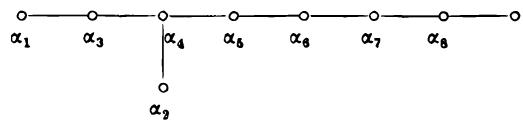
\includegraphics[keepaspectratio]{images/part002_295bff8e.jpg}}

\begin{enumerate}
\def\labelenumi{(\Alph{enumi})}
\setcounter{enumi}{21}
\tightlist
\item
  由于 \((\alpha |\alpha) = 2\) 对所有 \(\alpha \in \mathbb{R}\) 成立，所以 \(R^{\prime} = R\)。
\end{enumerate}

对于 \(\Phi_{\mathrm{R}}\)，根的长度平方为 \(\frac{1}{30}\)（ \(\S 1\)，第 12 号）。因此，\(\Phi_{\mathrm{R}}(x,y) = (x|y)/60\)，且 \(\gamma(\mathrm{R}) = 900\)（ \(\S 1\)，第 12 号，公式 (20)）。

\begin{enumerate}
\def\labelenumi{(\Roman{enumi})}
\setcounter{enumi}{5}
\tightlist
\item
  计算基本权得到
\end{enumerate}

\[
\begin{array}{l} \omega_ {1} = 2 \varepsilon_ {8} = 4 \alpha_ {1} + 5 \alpha_ {2} + 7 \alpha_ {3} + 10 \alpha_ {4} + 8 \alpha_ {5} + 6 \alpha_ {6} + 4 \alpha_ {7} + 2 \alpha_ {8} \\ \omega_ {2} = \frac {1}{2} (\varepsilon_ {1} + \varepsilon_ {2} + \varepsilon_ {3} + \varepsilon_ {4} + \varepsilon_ {5} + \varepsilon_ {6} + \varepsilon_ {7} + 5 \varepsilon_ {8}) \\ \qquad = 5 \alpha_ {1} + 8 \alpha_ {2} + 10 \alpha_ {3} + 15 \alpha_ {4} + 12 \alpha_ {5} + 9 \alpha_ {6} + 6 \alpha_ {7} + 3 \alpha_ {8} \\ \omega_ {3} = \frac {1}{2} (- \varepsilon_ {1} + \varepsilon_ {2} + \varepsilon_ {3} + \varepsilon_ {4} + \varepsilon_ {5} + \varepsilon_ {6} + \varepsilon_ {7} + 7 \varepsilon_ {8}) \\ \qquad = 7 \alpha_ {1} + 10 \alpha_ {2} + 14 \alpha_ {3} + 20 \alpha_ {4} + 16 \alpha_ {5} + 12 \alpha_ {6} + 8 \alpha_ {7} + 4 \alpha_ {8} \\ \omega_ {4} = \varepsilon_ {3} + \varepsilon_ {4} + \varepsilon_ {5} + \varepsilon_ {6} + \varepsilon_ {7} + 5 \varepsilon_ {8} \\ \qquad = 10 \alpha_ {1} + 15 \alpha_ {2} + 20 \alpha_ {3} + 30 \alpha_ {4} + 24 \alpha_ {5} + 18 \alpha_ {6} + 12 \alpha_ {7} + 6 \alpha_ {8} \\ \omega_ {5} = \varepsilon_ {4} + \varepsilon_ {5} + \varepsilon_ {6} + \varepsilon_ {7} + 4 \varepsilon_ {8} \\ \qquad = 8 \alpha_ {1} + 12 \alpha_ {2} + 16 \alpha_ {3} + 24 \alpha_ {4} + 20 \alpha_ {5} + 15 \alpha_ {6} + 10 \alpha_ {7} + 5 \alpha_ {8} \\ \omega_ {6} = \varepsilon_ {5} + \varepsilon_ {6} + \varepsilon_ {7} + 3 \varepsilon_ {8} \\ \qquad = 6 \alpha_ {1} + 9 \alpha_ {2} + 12 \alpha_ {3} + 18 \alpha_ {4} + 15 \alpha_ {5} + 12 \alpha_ {6} + 8 \alpha_ {7} + 4 \alpha_ {8} \\ \omega_ {7} = \varepsilon_ {6} + \varepsilon_ {7} + 2 \varepsilon_ {8} \\ \qquad = 4 \alpha_ {1} + 6 \alpha_ {2} + 8 \alpha_ {3} + 2 \alpha_ {4} + 10 \alpha_ {5} + 8 \alpha_ {6} + 6 \alpha_ {7} + 3 \alpha_ {8} \\ \omega_ {8} = \varepsilon_ {7} + \varepsilon_ {8} \\ \qquad = 5 \alpha_ {1} + 8 \alpha_ {2} + 10 \alpha_ {3} + 15 \alpha_ {4} + 12 \alpha_ {5} + 9 \alpha_ {6} + 6 \alpha_ {7} + 3 \alpha_ {8} = \tilde {\alpha}. \end{array}
\]

\begin{enumerate}
\def\labelenumi{(\Roman{enumi})}
\setcounter{enumi}{6}
\tightlist
\item
  正根之和的一半是基本权之和（§ 1，第 10 号，命题 29）；这给出
\end{enumerate}

\[
\begin{array}{r l} \rho & = \varepsilon_ {2} + 2 \varepsilon_ {3} + 3 \varepsilon_ {4} + 4 \varepsilon_ {5} + 5 \varepsilon_ {6} + 6 \varepsilon_ {7} + 23 \varepsilon_ {8} \\ & = 46 \alpha_ {1} + 68 \alpha_ {2} + 91 \alpha_ {3} + 135 \alpha_ {4} + 110 \alpha_ {5} + 84 \alpha_ {6} + 57 \alpha_ {7} + 29 \alpha_ {8}. \end{array}
\]

\begin{enumerate}
\def\labelenumi{(\Roman{enumi})}
\setcounter{enumi}{7}
\item
  群 \(Q(R)\) 由 \(\varepsilon_{i} \pm \varepsilon_{j}\) 和 \(\frac{1}{2} \sum_{i=1}^{8} \varepsilon_{i}\) 生成，并且等于 \(L_{3}\)（第 4 号）。因此，\(P(R)\)（与 \(Q(R^{\prime}) = Q(R) = L_{3}\) 关联）是 \(L_{3}\)（第 4 号）。连接指标为 1。
\item
  指数族有 8 项，由于 h = 30，与 30 互素的整数 1、7、11、13、17、19、23、29 必须出现在此族中；因此，这些就是 W(R) 的指数。
\item
  由 (IX) 以及第 V 章 § 6 第 2 号命题 3 的推论 1，得到 W(R) 的阶为
\end{enumerate}

\[
2. 8. 12. 14. 18. 20. 24. 30 = 2 ^ {14}. 3 ^ {5}. 5 ^ {2}. 7.
\]

\begin{enumerate}
\def\labelenumi{(\Roman{enumi})}
\setcounter{enumi}{10}
\tightlist
\item
  Dynkin 图的唯一自同构是恒等自同构，因为从分叉点发出的三条链长度各不相同。因此，\(A(R) = W(R)\) 且 \(w_{0} = -1\)。
\end{enumerate}

\subsection{\texorpdfstring{\(E_{7}\) 型系统}{E\_7 型系统}}

\begin{enumerate}
\def\labelenumi{(\Roman{enumi})}
\tightlist
\item
  以及 (II) 设 \(E = R^{8}\)，并令 \(R_{8}\) 为第 10 号在 E 中构造的根系。令 V 为 E 中由根 \(\alpha_{1}, \ldots, \alpha_{7}\)（它们属于 \(R_{8}\)）生成的超平面；它与第八个基本权 \(\omega = \varepsilon_{7} + \varepsilon_{8}\)（属于 \(R_{8}\)）正交。
\end{enumerate}

  令 \(R = R_{8} \cap V\)。则 \(R\) 是一个以 \((\alpha_{1}, \ldots, \alpha_{7})\) 为基的约化根系，参见 § 1，第 7 号，命题 20 的推论 4；因此，该系统为 \(E_{7}\) 型。其元素为：

\[
\begin{array}{c} \pm \varepsilon_ {i} \pm \varepsilon_ {j} (1 \leqslant i < j \leqslant 6), \quad \pm (\varepsilon_ {7} - \varepsilon_ {8}), \\ \pm \frac {1}{2} (\varepsilon_ {7} - \varepsilon_ {8} + \sum_ {i = 1} ^ {8} (- 1) ^ {\nu (i)} \varepsilon_ {i}) \quad \text { with } \sum_ {i = 1} ^ {8} \nu (i) \text { odd }. \end{array}
\]

根的数目为 \(n = 2 + \binom{6}{2}.4 + 2^6 = 126\)。正根为

\[
\pm \varepsilon_ {i} + \varepsilon_ {j} (1 \leqslant i <   j \leqslant 6). - \varepsilon_ {7} + \varepsilon_ {8},
\]

\[
\frac {1}{2} \left(- \varepsilon_ {7} + \varepsilon_ {8} + \sum_ {i = 1} ^ {6} (- 1) ^ {\nu (i)} \varepsilon_ {i}\right) \quad \text { with } \sum_ {i = 1} ^ {6} \nu (i) \text { odd }.
\]

\begin{enumerate}
\def\labelenumi{(\Roman{enumi})}
\setcounter{enumi}{2}
\item
  我们有 \(h = \frac{n}{l} = 18\)。
\item
  令 \(\tilde{\alpha} = \varepsilon_8 - \varepsilon_7 = 2\alpha_1 + 2\alpha_2 + 3\alpha_3 + 4\alpha_4 + 3\alpha_5 + 2\alpha_6 + \alpha_7\)，这是一个根。相对于 \((\alpha_i)\)，它的坐标之和为 \(17 = h - 1\)。因此它是最高根。它与 \(\alpha_i\)（\(2 \leqslant i \leqslant 7\)）正交，且 \((\tilde{\alpha}|\alpha_1) = 1\)。扩展 Dynkin 图为
\end{enumerate}

\pandocbounded{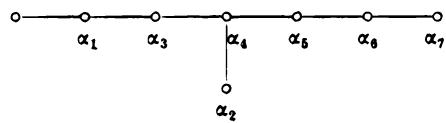
\includegraphics[keepaspectratio]{images/part002_8927380c.jpg}}

\begin{enumerate}
\def\labelenumi{(\Alph{enumi})}
\setcounter{enumi}{21}
\tightlist
\item
  由于 \((\alpha |\alpha) = 2\) 对所有 \(\alpha \in \mathbb{R}\) 成立，所以 \(R^{\prime} = R\)。
\end{enumerate}

对于 \(\Phi_{\mathrm{R}}\)，根的长度平方为 \(\frac{1}{18}\)，所以

\[
\Phi_ {\mathrm{R}} (x, y) = (x | y) / 36, \quad \text { and } \quad \gamma (\mathrm{R}) = 2 ^ {2}. 3 ^ {4}
\]

（§ 1，第 12 号，公式 (20)）。

\begin{enumerate}
\def\labelenumi{(\Roman{enumi})}
\setcounter{enumi}{5}
\tightlist
\item
  计算基本权得到
\end{enumerate}

\[
\begin{array}{r l} & {\omega_ {1} = \varepsilon_ {8} - \varepsilon_ {7} = 2 \alpha_ {1} + 2 \alpha_ {2} + 3 \alpha_ {3} + 4 \alpha_ {4} + 3 \alpha_ {5} + 2 \alpha_ {6} + \alpha_ {7}} \\ & {\omega_ {2} = \frac {1}{2} (\varepsilon_ {1} + \varepsilon_ {2} + \varepsilon_ {3} + \varepsilon_ {4} + \varepsilon_ {5} + \varepsilon_ {6} - 2 \varepsilon_ {7} + 2 \varepsilon_ {8})} \\ & {\qquad = \frac {1}{2} (4 \alpha_ {1} + 7 \alpha_ {2} + 8 \alpha_ {3} + 12 \alpha_ {4} + 9 \alpha_ {5} + 8 \alpha_ {6} + 3 \alpha_ {7})} \\ & {\omega_ {3} = \frac {1}{2} (- \varepsilon_ {1} + \varepsilon_ {2} + \varepsilon_ {3} + \varepsilon_ {4} + \varepsilon_ {5} + \varepsilon_ {6} - 3 \varepsilon_ {7} + 3 \varepsilon_ {8})} \\ & {\qquad = 3 \alpha_ {1} + 4 \alpha_ {2} + 6 \alpha_ {3} + 8 \alpha_ {4} + 6 \alpha_ {5} + 4 \alpha_ {6} + 2 \alpha_ {7}} \\ & {\omega_ {4} = \varepsilon_ {3} + \varepsilon_ {4} + \varepsilon_ {5} + \varepsilon_ {6} + 2 (\varepsilon_ {8} - \varepsilon_ {7})} \\ & {\qquad = 4 \alpha_ {1} + 6 \alpha_ {2} + 8 \alpha_ {3} + 12 \alpha_ {4} + 9 \alpha_ {5} + 6 \alpha_ {6} + 3 \alpha_ {7}} \\ & {\omega_ {5} = \varepsilon_ {4} + \varepsilon_ {5} + \varepsilon_ {6} + \frac {3}{2} (\varepsilon_ {8} - \varepsilon_ {7})} \\ & {\qquad = \frac {1}{2} (6 \alpha_ {1} + 9 \alpha_ {2} + 12 \alpha_ {3} + 18 \alpha_ {4} + 15 \alpha_ {5} + 10 \alpha_ {6} + 5 \alpha_ {7})} \\ & {\omega_ {6} = \varepsilon_ {5} + \varepsilon_ {6} - \varepsilon_ {7} + \varepsilon_ {8}} \\ & {\qquad = 2 \alpha_ {1} + 3 \alpha_ {2} + 4 \alpha_ {3} + 6 \alpha_ {4} + 5 \alpha_ {5} + 4 \alpha_ {6} + 2 \alpha_ {7}} \\ & {\omega_ {7} = \varepsilon_ {6} + \frac {1}{2} (\varepsilon_ {8} - \varepsilon_ {7})} \\ & {\qquad = \frac {1}{2} (2 \alpha_ {1} + 3 \alpha_ {2} + 4 \alpha_ {3} + 6 \alpha_ {4} + 5 \alpha_ {5} + 4 \alpha_ {6} + 3 \alpha_ {7}).} \end{array}
\]

\begin{enumerate}
\def\labelenumi{(\Roman{enumi})}
\setcounter{enumi}{6}
\tightlist
\item
  正根之和 \(2\rho\) 等于 \(2\sum_{i=1}^{7}\omega_i\)（§ 1，第 10 号，命题 29），所以
\end{enumerate}

\[
\begin{array}{r l} 2 \rho & = 2 \varepsilon_ {2} + 4 \varepsilon_ {3} + 6 \varepsilon_ {4} + 8 \varepsilon_ {5} + 10 \varepsilon_ {6} - 17 \varepsilon_ {7} + 17 \varepsilon_ {8} \\ & = 34 \alpha_ {1} + 49 \alpha_ {2} + 66 \alpha_ {3} + 96 \alpha_ {4} + 75 \alpha_ {5} + 52 \alpha_ {6} + 27 \alpha_ {7}. \end{array}
\]

\begin{enumerate}
\def\labelenumi{(\Roman{enumi})}
\setcounter{enumi}{7}
\tightlist
\item
  由第 10 号 (VIII) 及 § 1，第 10 号，命题 28，有
\end{enumerate}

\[
\mathrm{Q} (\mathrm{R}) = \mathrm{Q} (\mathrm{R} _ {8}) \cap \mathrm{V} = \mathrm{L} _ {3} \cap \mathrm{V} \quad \text { and } \quad \mathrm{P} (\mathrm{R}) = p (\mathrm{P} (\mathrm{R} _ {8})) = p (\mathrm{L} _ {3}),
\]

其中 p 表示 E 到 V 的正交投影。群 \(Q(R)\) 的基为 \((\alpha_{1},\ldots,\alpha_{7})\)；群 \(P(R)\) 由 \(Q(R)\) 和

\[
p (\alpha_ {8}) = \alpha_ {8} - \frac {1}{2} \omega .
\]

我们有 \(\omega\in\mathrm{P}(\mathrm{R}_{8})\)，\(\frac{1}{2}\omega\notin\mathrm{P}(\mathrm{R}_{8})\)，所以 \(2p(\alpha_{8})\in\mathrm{Q}(\mathrm{R})\) 而 \(p(\alpha_{8})\notin\mathrm{Q}(\mathrm{R})\)。因此，\(\mathrm{P}(\mathrm{R})/\mathrm{Q}(\mathrm{R})\) 同构于 Z/2Z，并由例如 \(\omega_{7}\) 的像生成。

连接指标为 2。

\begin{enumerate}
\def\labelenumi{(\Roman{enumi})}
\setcounter{enumi}{8}
\tightlist
\item
  \(W(R)\) 的指数序列有 7 项。与 \(h = 18\) 互素的数 1、5、7、11、13、17 出现在此序列中。最后一个指数 \(m\) 必须满足 \(m + m = 18\)（第 V 章，§ 6，第 2 号，公式 (2)）。因此，指数序列为
\end{enumerate}

\[
1, 5, 7, 9, 11, 13, 17.
\]

\begin{enumerate}
\def\labelenumi{(\Alph{enumi})}
\setcounter{enumi}{23}
\tightlist
\item
  由 (IX) 及第 V 章 § 6 第 2 号命题 3 的推论 1，得到 W(R) 的阶为
\end{enumerate}

\[
2. 6. 8. 10. 12. 14. 18 = 2 ^ {10}. 3 ^ {4}. 5. 7.
\]

\begin{enumerate}
\def\labelenumi{(\Roman{enumi})}
\setcounter{enumi}{10}
\item
  Dynkin 图的唯一自同构是恒等自同构，所以 \(\mathbf{A}(\mathbf{R}) = \mathbf{W}(\mathbf{R})\) 且 \(w_0 = -1\)。
\item
  \(\mathrm{P}(\mathrm{R}^{-})/\mathrm{Q}(\mathrm{R}^{-})\) 只有一个非单位元。它互换对应于 \(\alpha_{0}\) 和 \(\alpha_{7}\)、\(\alpha_{1}\) 和 \(\alpha_{6}\)、\(\alpha_{3}\) 和 \(\alpha_{5}\) 的顶点，并固定 \(\alpha_{2}\) 和 \(\alpha_{4}\)。
\end{enumerate}

\subsection{\texorpdfstring{\(E_{6}\) 型系统}{E\_6 型系统}}

\begin{enumerate}
\def\labelenumi{(\Roman{enumi})}
\tightlist
\item
  以及 (II) 设 \(E = R^{8}\) ，并令 \(R_{8}\) 为第 10 号中构造的 E 中的根系。令 V 为 E 中由根 \(\alpha_{1}, \ldots, \alpha_{6}\)（属于 \(R_{8}\)）所生成的向量子空间；它是由最后两个基本权 \(\omega = \varepsilon_{7} + \varepsilon_{8}\) 和 \(\pi = \varepsilon_{6} + \varepsilon_{7} + 2\varepsilon_{8}\)（属于 \(R_{8}\)）所生成平面的正交补。
\end{enumerate}

令 \(R = R_{8} \cap V\) 。这是一个以 \((\alpha_{1}, \ldots, \alpha_{6})\) 为基的约化根系，因而是 \(E_{6}\) 型的根系。其元素为：

\[
\begin{array}{c} \pm \varepsilon_ {i} \pm \varepsilon_ {j} (1 \leqslant i <   j \leqslant 5), \\ \pm \frac {1}{2} (\varepsilon_ {8} - \varepsilon_ {7} - \varepsilon_ {6} + \sum_ {i = 1} ^ {5} (- 1) ^ {\nu (i)} \varepsilon_ {i}) \text {with} \sum_ {i = 1} ^ {5} \nu (i) \text {even.} \end{array}
\]

根的数目为 \(n = \binom{5}{2}.4 + 2^5 = 72\) 。正根为

\[
\pm \varepsilon_ {i} + \varepsilon_ {j} (1 \leqslant i <   j \leqslant 5),
\]

\[
\frac {1}{2} \left(\varepsilon_ {8} - \varepsilon_ {7} - \varepsilon_ {6} + \sum_ {i = 1} ^ {5} (- 1) ^ {\nu (i)} \varepsilon_ {i}\right) \text {with} \sum_ {i = 1} ^ {5} \nu (i) \text {even}.
\]

\begin{enumerate}
\def\labelenumi{(\Roman{enumi})}
\setcounter{enumi}{2}
\item
  我们有 \(h = \frac{n}{6} = 12\) 。
\item
  令
\end{enumerate}

\[
\begin{array}{r l} \tilde {\alpha} & = \frac {1}{2} (\varepsilon_ {1} + \varepsilon_ {2} + \varepsilon_ {3} + \varepsilon_ {4} + \varepsilon_ {5} - \varepsilon_ {6} - \varepsilon_ {7} + \varepsilon_ {8}) \\ & = \alpha_ {1} + 2 \alpha_ {2} + 2 \alpha_ {3} + 3 \alpha_ {4} + 2 \alpha_ {5} + \alpha_ {6}, \end{array}
\]

这是一个根。相对于 \((\alpha_{i})\) ，其坐标之和为 11 = h - 1，因此 \(\tilde{\alpha}\) 是最高根。它与 \(\alpha_{1}, \alpha_{3}, \alpha_{4}, \alpha_{5}, \alpha_{6}\) 正交，且 \((\tilde{\alpha}|\alpha_{2}) = 1\) 。扩充的 Dynkin 图为

\pandocbounded{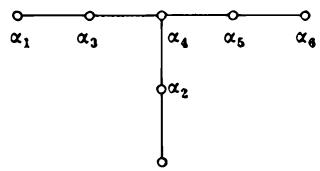
\includegraphics[keepaspectratio]{images/part002_9f0044a9.jpg}}

\begin{enumerate}
\def\labelenumi{(\Alph{enumi})}
\setcounter{enumi}{21}
\tightlist
\item
  由于 \((\alpha |\alpha) = 2\) 对所有 \(\alpha \in \mathbb{R}\) 成立，所以 \(\mathbb{R}^{\sim} = \mathbb{R}\) 。对于 \(\Phi_{\mathbb{R}}\) ，根的长度平方为 \(\frac{1}{12}\) ，因此
\end{enumerate}

\[
\Phi_ {\mathrm{R}} (x, y) = (x | y) / 24, \quad \text { and } \quad \gamma (\mathrm{R}) = 144.
\]

\begin{enumerate}
\def\labelenumi{(\Roman{enumi})}
\setcounter{enumi}{5}
\tightlist
\item
  计算基本权得到：
\end{enumerate}

\[
\begin{array}{l} \omega_ {1} = \frac {2}{3} (\varepsilon_ {8} - \varepsilon_ {7} - \varepsilon_ {6}) = \frac {1}{3} (4 \alpha_ {1} + 3 \alpha_ {2} + 5 \alpha_ {3} + 6 \alpha_ {4} + 4 \alpha_ {5} + 2 \alpha_ {6}) \\ \omega_ {2} = \frac {1}{2} (\varepsilon_ {1} + \varepsilon_ {2} + \varepsilon_ {3} + \varepsilon_ {4} + \varepsilon_ {5} - \varepsilon_ {6} - \varepsilon_ {7} + \varepsilon_ {8}) \\ \quad = \alpha_ {1} + 2 \alpha_ {2} + 2 \alpha_ {3} + 3 \alpha_ {4} + 2 \alpha_ {5} + \alpha_ {6} = \tilde {\alpha} \\ \omega_ {3} = \frac {5}{6} (\varepsilon_ {8} - \varepsilon_ {7} - \varepsilon_ {6}) + \frac {1}{2} (- \varepsilon_ {1} + \varepsilon_ {2} + \varepsilon_ {3} + \varepsilon_ {4} + \varepsilon_ {5}) \\ \quad = \frac {1}{3} (5 \alpha_ {1} + 6 \alpha_ {2} + 10 \alpha_ {3} + 12 \alpha_ {4} + 8 \alpha_ {5} + 4 \alpha_ {6}) \\ \omega_ {4} = \varepsilon_ {3} + \varepsilon_ {4} + \varepsilon_ {5} - \varepsilon_ {6} - \varepsilon_ {7} + \varepsilon_ {8} \\ \quad = 2 \alpha_ {1} + 3 \alpha_ {2} + 4 \alpha_ {3} + 6 \alpha_ {4} + 4 \alpha_ {5} + 2 \alpha_ {6} \\ \omega_ {5} = \frac {2}{3} (\varepsilon_ {8} - \varepsilon_ {7} - \varepsilon_ {6}) + \varepsilon_ {4} + \varepsilon_ {5} \\ \quad = \frac {1}{3} (4 \alpha_ {1} + 6 \alpha_ {2} + 8 \alpha_ {3} + 12 \alpha_ {4} + 10 \alpha_ {5} + 5 \alpha_ {6}) \\ \omega_ {6} = \frac {1}{3} (\varepsilon_ {8} - \varepsilon_ {7} - \varepsilon_ {6}) + \varepsilon_ {5} \\ \quad = \frac {1}{3} (2 \alpha_ {1} + 3 \alpha_ {2} + 4 \alpha_ {3} + 6 \alpha_ {4} + 5 \alpha_ {5} + 4 \alpha_ {6}). \end{array}
\]

\begin{enumerate}
\def\labelenumi{(\Roman{enumi})}
\setcounter{enumi}{6}
\tightlist
\item
  正根之和的一半是 \(\sum_{i=1}^{6} \omega_i\) ，所以
\end{enumerate}

\[
\begin{array}{r l} \rho & = \varepsilon_ {2} + 2 \varepsilon_ {3} + 3 \varepsilon_ {4} + 4 \varepsilon_ {5} + 4 (\varepsilon_ {8} - \varepsilon_ {7} - \varepsilon_ {6}) \\ & = 8 \alpha_ {1} + 11 \alpha_ {2} + 15 \alpha_ {3} + 21 \alpha_ {4} + 15 \alpha_ {5} + 8 \alpha_ {6}. \end{array}
\]

\begin{enumerate}
\def\labelenumi{(\Roman{enumi})}
\setcounter{enumi}{7}
\tightlist
\item
  由第 10 号 (VIII) 及 § 1，第 10 号，命题 28，
\end{enumerate}

\[
\mathrm{Q} (\mathrm{R}) = \mathrm{Q} (\mathrm{R} _ {8}) \cap \mathrm{V} = \mathrm{L} _ {3} \cap \mathrm{V} \quad \text { and } \quad \mathrm{P} (\mathrm{R}) = p (\mathrm{P} (\mathrm{R} _ {8})) = p (\mathrm{L} _ {3}),
\]

其中 p 表示从 E 到 V 的正交投影。我们有

\[
p (\alpha_ {7}) = \alpha_ {7} - \frac {2}{3} \pi + \omega , \quad p (\alpha_ {8}) = \alpha_ {8} + \pi - 2 \omega .
\]

群 \(Q(R)\) 的基为 \((\alpha_{1},\ldots,\alpha_{6})\) 。群 \(P(R)\) 由 \(Q(R)\) 和 \(p(\alpha_{7})\) 生成，因为 \(p(\alpha_{8})\in P(R_{8})\cap V=Q(R_{8})\cap V=Q(R)\) 。我们有 \(3p(\alpha_{7})\in Q(R)\) 且 \(p(\alpha_{7})\notin Q(R)\) 。因此，群 \(P(R)/Q(R)\) 同构于 Z/3Z；例如，它由 \(\omega_{6}\) 的像生成。

连通指标为 3。

\begin{enumerate}
\def\labelenumi{(\Roman{enumi})}
\setcounter{enumi}{8}
\tightlist
\item
  (IX) 和 (X) 由 § 2，第 4 号，命题 7，Weyl 群的阶为 6!1.2.2.3.2.1.3 = \(2^{7}.3^{4}.5\) 。指数序列在 1 与 11 之间有 6 项，并包含与 12 互素的整数 1、5、7、11。其他指数 \(m, m'\) 是满足
\end{enumerate}

\[
m + m ^ {\prime} = 12.
\]

\[
(m + 1) \left(m ^ {\prime} + 1\right) (1 + 1) (5 + 1) (7 + 1) (11 + 1) = 2 ^ {7}. 3 ^ {4}. 5,
\]

根据第 V 章 § 6，第 2 号，公式 (2) 以及命题 3 的推论 1。第二个关系给出 \((m + 1)(m' + 1) = 45\) ，又因 \(m + m' + 2 = 14\) ，得到 \(m = 4\) ，\(m' = 8\) 。因此，指数序列为

\[
1, 4, 5, 7, 8, 11.
\]

\begin{enumerate}
\def\labelenumi{(\Roman{enumi})}
\setcounter{enumi}{10}
\tightlist
\item
  (XI) 和 (XII) 由于所有根的长度都相同，Dynkin 图的自同构就是底层图的自同构。除恒等自同构外，只有自同构 \(\varepsilon\) 将 \(\alpha_{1},\alpha_{3},\alpha_{4},\alpha_{5},\alpha_{6},\) \(\alpha_{2}\) 分别变为 \(\alpha_{6},\alpha_{5},\alpha_{4},\alpha_{3},\alpha_{1},\alpha_{2}\) 。因此，\(\mathrm{A(R) / W(R)}\) 同构于 \(\mathbf{Z} / 2\mathbf{Z}\) ；由于 \(-1\in \mathrm{W(R)}\) （第 V 章 §6，第 2 号，命题 3 的推论 3），\(\mathrm{A(R)}\) 同构于 \(\mathrm{W(R)}\times \{1, - 1\}\) ，且可将 \(w_0\) 认作 \(-\varepsilon\) 。由此，\(\mathrm{A(R) / W(R)}\) 的非恒等元素定义了自同构 \(x\mapsto -x\)，该自同构作用于 \(\mathrm{P(R^{\prime}) / Q(R^{\prime})}\)。
\end{enumerate}

此外，\(P(R^{-})/Q(R^{-})\) 有两个阶为 3 的非恒等元素。它们定义了扩充 Dynkin 图的两个三阶自同构。

\subsection{\texorpdfstring{\(G_{2}\) 型系统}{G\_2 型系统}}

\begin{enumerate}
\def\labelenumi{(\Roman{enumi})}
\tightlist
\item
  令 E 为 \(R^{3}\) 中方程为
\end{enumerate}

\[
\xi_ {1} + \xi_ {2} + \xi_ {3} = 0.
\]

  令 \(R\) 为由 \(\alpha \in L_0 \cap V\) 且满足 \((\alpha | \alpha) = 2\) 或 \((\alpha | \alpha) = 6\) 的元素组成的集合。\(R\) 的元素为

\[
\begin{array}{c} \pm (\varepsilon_ {1} - \varepsilon_ {2}), \quad \pm (\varepsilon_ {1} - \varepsilon_ {3}), \quad \pm (\varepsilon_ {2} - \varepsilon_ {3}), \quad \pm (2 \varepsilon_ {1} - \varepsilon_ {2} - \varepsilon_ {3}), \\ \pm (2 \varepsilon_ {2} - \varepsilon_ {1} - \varepsilon_ {3}), \quad \pm (2 \varepsilon_ {3} - \varepsilon_ {1} - \varepsilon_ {2}). \end{array}
\]

  于是，R 生成 V，且 \(\frac{2(\alpha|\beta)}{(\beta|\beta)}\in\mathbf{Z}\) 对所有 \(\alpha,\beta\in R\) 成立：当 \(\beta=\pm(\varepsilon_{i}-\varepsilon_{j})\) 且 \(i\neq j\) 时这显然成立；例如，当 \(\beta=2\varepsilon_{1}-\varepsilon_{2}-\varepsilon_{3}\) 时，我们有 \((\alpha|\beta)\in3\mathbf{Z}\) ，断言同样成立。因此，R 是 V 中的约化根系。根的数目为 n=12。

\begin{enumerate}
\def\labelenumi{(\Roman{enumi})}
\setcounter{enumi}{1}
\tightlist
\item
  置 \(\alpha_{1} = \varepsilon_{1} - \varepsilon_{2},\alpha_{2} = -2\varepsilon_{1} + \varepsilon_{2} + \varepsilon_{3}\) 。则这些根为
\end{enumerate}

\[
\begin{array}{r l} & {\pm \alpha_ {1}, \quad \pm (\alpha_ {1} + \alpha_ {2}), \quad \pm (2 \alpha_ {1} + \alpha_ {2}), \quad \pm \alpha_ {2},} \\ & {\qquad \pm (3 \alpha_ {1} + \alpha_ {2}), \quad \pm (3 \alpha_ {1} + 2 \alpha_ {2}).} \end{array}
\]

因此，\((\alpha_{1},\alpha_{2})\) 是 \(R\) 的一个基。我们有 \(\| \alpha_{1}\|^{2} = 2,\| \alpha_{2}\|^{2} = 6.\) \((\alpha_{1}|\alpha_{2}) = -3,\) 所以 \(R\) 是 \(G_{2}\) 型系统。正根为 \(\alpha_{1},\alpha_{1} + \alpha_{2},2\alpha_{1} + \alpha_{2},\) \(3\alpha_{1} + \alpha_{2},3\alpha_{1} + 2\alpha_{2}\) 。

\begin{enumerate}
\def\labelenumi{(\Roman{enumi})}
\setcounter{enumi}{2}
\item
  我们有 \(h = \frac{n}{2} = 6\) 。
\item
  最高根为 \(\tilde{\alpha} = 3\alpha_{1} + 2\alpha_{2} = -\varepsilon_{1} - \varepsilon_{2} + 2\varepsilon_{3}\) 。我们有 \((\tilde{\alpha}|\alpha_{1}) = 0, (\tilde{\alpha}|\alpha_{2}) = 3\) 。扩充的 Dynkin 图为
\end{enumerate}

\[
\alpha_ {1} \quad \alpha_ {2}
\]

\begin{enumerate}
\def\labelenumi{(\Alph{enumi})}
\setcounter{enumi}{21}
\tightlist
\item
  逆系统是下列向量集：
\end{enumerate}

\[
\begin{array}{l} \pm \alpha_ {1}, \quad \pm (\alpha_ {1} + \alpha_ {2}), \quad \pm (2 \alpha_ {1} + \alpha_ {2}), \quad \pm \frac {1}{3} \alpha_ {2}, \\ \qquad \pm \frac {1}{3} (3 \alpha_ {1} + \alpha_ {2}), \quad \pm \frac {1}{3} (3 \alpha_ {1} + 2 \alpha_ {2}). \end{array}
\]

  有 10 个根不与 \(\alpha_{1}\) 正交；其中 4 个根满足 \(n(\beta, \alpha_{1}) = \pm 1\) ，另外 4 个满足 \(n(\beta, \alpha_{1}) = \pm 3\) ，另有 \(n(\beta, \alpha_{1}) = \pm 2\) 的根满足 \(\beta = \pm \alpha_{1}\) 。因此，\(\alpha_{1}\) 在 \(\Phi_{\mathbb{R}}\) 中的长度平方为 \(4(4.1 + 4.9 + 2.4)^{-1} = \frac{1}{12}\) 。从而 \(\Phi_{\mathbb{R}}(x, y) = (x|y)/24\) 。现在对 \(x = y = \alpha_{1}\) 应用 §1 第 12 号的公式 (18)，得到

\[
2 + 4. \frac {1}{4} + 4. \frac {1}{4} = \gamma (\mathrm{R}). \frac {1}{12}
\]

所以 \(\gamma (\mathbb{R}) = 48\)

\begin{enumerate}
\def\labelenumi{(\Roman{enumi})}
\setcounter{enumi}{5}
\tightlist
\item
  (VI) 和 (VII) 正根之和的一半为
\end{enumerate}

\[
\rho = 5 \alpha_ {1} + 3 \alpha_ {2}.
\]

基本权 \(\omega_{1}\) 和 \(\omega_{2}\) 分别与 \(\alpha_{2}\) 和 \(\alpha_{1}\) 正交，因而分别与 \(2\alpha_{1} + \alpha_{2}\) 和 \(3\alpha_{1} + 2\alpha_{2}\) 成比例。我们有

\[
\omega_ {1} + \omega_ {2} = \rho = 5 \alpha_ {1} + 3 \alpha_ {2} = (2 \alpha_ {1} + \alpha_ {2}) + (3 \alpha_ {1} + 2 \alpha_ {2}).
\]

因此，

\[
\omega_ {1} = 2 \alpha_ {1} + \alpha_ {2}, \quad \omega_ {2} = 3 \alpha_ {1} + 2 \alpha_ {2} = \tilde {\alpha}.
\]

\begin{enumerate}
\def\labelenumi{(\Roman{enumi})}
\setcounter{enumi}{7}
\item
  例如，Q(R) 由 \(\varepsilon_{1}-\varepsilon_{2}\) 和 \(\varepsilon_{1}-\varepsilon_{3}\) 生成。由 (VI) 和 (VII)，P(R) = Q(R)。连通指标为 1。
\item
  指数族有 2 项：由于 1 和 \(h - 1 = 5\) 是指数，它们就是全部指数。
\item
  我们有 \((\alpha_{1},\alpha_{2}) = \frac{5\pi}{6}\) ，所以 \(\mathrm{W}(\mathbb{R})\) 同构于阶为 12 的二面体群。
\item
  Dynkin 图的唯一自同构是恒等自同构，所以 \(A(R) = W(R)\) 且 \(w_{0} = -1\) 。
\end{enumerate}

\subsection{不可约非约化根系}

利用 §1 第 4 号的命题 13 和 14，可以从不可约约化根系得到不可约非约化根系。对每个整数 \(l \geqslant 1\) ，存在一个秩为 \(l\) 的不可约非约化根系，且在同构意义下唯一：令 \(R\) 为 \(B_l\) 型根系。令 A 为 \(R\) 的最短根的集合；取 \(R\) 与 \(2A\) 的并。采用第 5 号的记号，我们得到 \(2l(l + 1)\) 个向量

\[
\pm \varepsilon_ {i}, \quad \pm 2 \varepsilon_ {i}, \quad \varepsilon_ {i} \pm \varepsilon_ {j} (i <   j).
\]

\exercisesection{§ 1 的习题}

下文考虑的所有根系都相对于实向量空间。我们用 \((x|y)\) 表示在 Weyl 群下不变的标量积（参见第 3 号）。

\begin{enumerate}
\def\labelenumi{\arabic{enumi})}
\item
  令 \(\mathbb{R}\) 为根系，\(\mathbb{R} = \mathbb{R}_1 \cup \mathbb{R}_2\) 为 \(\mathbb{R}\) 的一个划分。假设，当 \(x, y\) 是 \(\mathbb{R}_i\) 的两个元素且 \(x + y\)（分别为 \(x - y\)）是一个根时，就有 \(x + y \in \mathbb{R}_i\)（分别为 \(x - y \in \mathbb{R}_i\)），其中 \(i = 1, 2\)。那么，\(\mathbb{R}\) 是 \(\mathbb{R}_1\) 与 \(\mathbb{R}_2\) 的直和。（利用第 3 号定理 1 的推论，证明若 \(x \in \mathbb{R}_1\) 且 \(y \in \mathbb{R}_2\)，则 \((x|y) = 0\)。）
\item
  令 R 为根系，\(\alpha\) 和 \(\beta\) 为两个根。若 t 是一个标量且 \(\beta + t\alpha \in R\) ，则 \(2t \in Z\) 。（因为 \(n(\beta + t\alpha, \alpha) = n(\beta, \alpha) + 2t\) 。）若 \(\alpha\) 不可整除，则 \(t \in Z\) 。（否则利用命题 9 证明存在一个根 \(\gamma\)，它与 \(\alpha\) 正交，使得 \(\gamma + \frac{1}{2}\alpha \in R\)：于是 \((\gamma + \frac{1}{2}\alpha|\alpha) > 0\) ，所以 \(\frac{1}{2}\alpha \in R\)。）
\item
  令 R 为 V 中的不可约非约化根系。V 上存在一个非退化对称双线性型 \(\Phi\)，使得当将 V 与 \(V^{*}\) 通过 \(\Phi\) 识别时，有 \(R = R^{-}\)。（利用命题 13。）
\item
  令 \(\Gamma\) 为有限秩自由 \(\mathbf{Z}\)-模，其秩为 \(l\)，\(\Gamma^{*}\) 为其对偶 \(\mathbf{Z}\)-模，I 为有限指标集，\((x_{i}, x_{i}^{*})_{i \in \mathbf{I}}\) 为 \(\Gamma \times \Gamma^{*}\) 中的元素族，且满足 \(\langle x_{i}, x_{i}^{*} \rangle = 2\) 对所有 \(i \in \mathbf{I}\) 成立，\(s_{i} = s_{x_{i}, x_{i}^{*}}\)。令 \(\mathbf{V}\) 为实向量空间 \(\Gamma \otimes_{\mathbf{Z}} \mathbf{R}\)，其对偶 \(\mathbf{V}^{*}\) 可与 \(\Gamma^{*} \otimes_{\mathbf{Z}} \mathbf{R}\) 识别。我们也用 \(s_{i}\) 表示反射 \(s_{i} \otimes 1\) 在 \(\mathbf{V}\) 中的作用。令 \(\mathbf{R}\)（分别为 \(\mathbf{R}'\)）为 \(x_{i}\)（分别为 \(x_{i}^{*}\)）的集合。令 \(\mathbf{E}\)（分别为 \(\mathbf{E}'\)）为 \(\mathbf{V}\)（分别为 \(\mathbf{V}^{*}\)）中由 \(\mathbf{R}\)（分别为 \(\mathbf{R}'\)）生成的子空间。假设 \(s_{i}(\mathbf{R}) = \mathbf{R}\) 对所有 \(i\) 成立。那么，\(\mathbf{R}\) 是 \(\mathbf{E}\) 中的根系。\(\mathbf{E}'\) 可自然地识别为 \(\mathbf{E}\) 的对偶，且 \(x_{i}^{*}\) 可与 \(x_{i}^{-}\) 识别，对所有 \(i\) 均如此。若 \(\mathbf{F}\)（分别为 \(\mathbf{F}'\)）是 \(\mathbf{V}\)（分别为 \(\mathbf{V}^{*}\)）中在所有 \(s_{i}\)（分别为 \(^t s_{i}\)）下不变的点所成的子空间，则 \(\Gamma \cap \mathbf{F}\)（分别为 \(\Gamma^{*} \cap \mathbf{F}'\)）生成 \(\mathbf{F}\)（分别为 \(\mathbf{F}'\)）。若置 \(\Gamma_{1} = (\Gamma \cap \mathbf{E}) \oplus (\Gamma \cap \mathbf{F})\)（分别为 \(\Gamma_{1}^{*} = (\Gamma^{*} \cap \mathbf{E}') \oplus (\Gamma^{*} \cap \mathbf{F}')\)），则 \(\Gamma / \Gamma_{1}\) 与 \(\Gamma^{*} / \Gamma_{1}^{*}\) 是同构的有限群。
\item
  令 \(R\) 为不可约根系。对任意 \(\beta \in R\)，
\end{enumerate}

\[
16 \gamma (\mathrm{R}) = (\sum_ {\alpha \in \mathrm{R}} n (\alpha , \beta) ^ {2}) (\sum_ {\alpha \in \mathrm{R}} n (\beta , \alpha) ^ {2})
\]

从而 \(\gamma (\mathbb{R}) = \gamma (\lambda R)\) 对任意非零标量 \(\lambda\) 成立。（利用第 12 号的公式 (17) 和 (19)。）

\begin{enumerate}
\def\labelenumi{\arabic{enumi})}
\setcounter{enumi}{5}
\tightlist
\item
  \begin{enumerate}
  \def\labelenumii{\alph{enumii})}
  \tightlist
  \item
    令 A 为有限型阿贝尔群，T 为 A 的一个不含 0 的有限子集。存在 A 的有限指数子群 H，使得 \(H \cap T = \varnothing\)。（令 \(t \in T\)。利用有限型阿贝尔群的结构，构造 A 的一个不含 t 的有限指数子群。然后对 \(\text{Card}(T)\) 作归纳。）
  \end{enumerate}
\end{enumerate}

\begin{enumerate}
\def\labelenumi{\alph{enumi})}
\setcounter{enumi}{1}
\tightlist
\item
  令 R 为根系，P 为 R 的一个闭对称子集。存在 Q(R) 的有限指数子群 H，使得 \(P = H \cap R\)。（对 Q(R) 中由 P 生成的子群取商，并利用 a) 和命题 23。）
\end{enumerate}

\begin{enumerate}
\def\labelenumi{\arabic{enumi})}
\setcounter{enumi}{6}
\item
  根系的连通指标等于其 Cartan 矩阵的行列式。（利用第 10 号的公式 (14)。另一方面证明：在带有标量积的实向量空间中，若 \((\varepsilon_1, \ldots, \varepsilon_n), (\varepsilon_1', \ldots, \varepsilon_n')\) 是满足 \((\varepsilon_i | \varepsilon_j') = \delta_{ij}\) 的两个基，则 \(\det_{(\varepsilon_1, \ldots, \varepsilon_n)} (\varepsilon_1', \ldots, \varepsilon_n') > 0\)。）
\item
  令 R 为约化根系，C 为一个室，\(2\sigma\) 为 \(R^{-}\) 的正元素之和，\(P'(R)\) 为满足 \(x \in P(R)\) 且 \(\langle x, \sigma \rangle \in Z\) 的集合。于是，\(Q(R) \subseteq P'(R) \subseteq P(R)\)，且 \(P(R)/P'(R)\) 的阶为 1 或 2。令 \((\beta_{1}, \ldots, \beta_{l})\) 为与 C 对应的 \(R^{-}\) 的基，并置 \(2\sigma = n_{1}\beta_{1} + \cdots + n_{l}\beta_{l}\)，其中 \(n_{i}\) 是 \textgreater0 的整数。则 \(P(R) = P'(R)\) 当且仅当所有 \(n_{i}\) 都是偶数。
\item
  令 \(\mathbb{R}\) 为根系，\(\mathbb{C}\) 为一个室。置 \(\mathrm{B}(\mathbb{C}) = \{\alpha_1, \ldots, \alpha_l\}\)，
\end{enumerate}

\[
\mathrm{R} _ {+} (\mathrm{C}) = \left\{\alpha_ {1}, \dots , \alpha_ {l}, \alpha_ {l + 1}, \dots , \alpha_ {s} \right\}
\]

（其中 \(\alpha_{i}\) 两两不同），并令 \(\alpha = \alpha_{1} + \dots +\alpha_{s}\)。

\begin{enumerate}
\def\labelenumi{\alph{enumi})}
\tightlist
\item
  对 \(i = 1, 2, \ldots, s\) ，置 \(\varepsilon_{i} = \pm 1\)。令 \(\alpha^{*} = \varepsilon_{1}\alpha_{1} + \cdots + \varepsilon_{s}\alpha_{s}\)。若 \((\alpha^{*}|\alpha_{i}) > 0\) 对 \(i = 1, \ldots, l\) 成立，则 \(\alpha^{*} = \alpha\) 且对所有 i 都有 \(\varepsilon_{i} = 1\)。（令 \(\gamma\)（分别为 \(\delta\)）为 \(\alpha_{i}\) 之和，其中 \(\varepsilon_{i} = 1\)（分别为 -1）。则 \((\gamma|\alpha_{i}) - (\delta|\alpha_{i}) > 0\)，\((\gamma|\alpha_{i}) + (\delta|\alpha_{i}) = (\alpha_{i}|\alpha_{i})\)，所以
\end{enumerate}

\(2(\gamma|\alpha_{i})>(\alpha_{i}|\alpha_{i});\) 由于 \(2(\gamma|\alpha_{i}) / (\alpha_{i}|\alpha_{i})\in \mathbf{Z},(\gamma |\alpha_{i})\geqslant (\alpha_{i}|\alpha_{i}) = (\alpha |\alpha_{i}),\) 因而 \(\gamma -\alpha \in \overline{\mathrm{C}}. \gamma \geqslant \alpha ,\) \(\gamma = \alpha\) 且 \(\delta = 0.)\)

\begin{enumerate}
\def\labelenumi{\alph{enumi})}
\setcounter{enumi}{1}
\tightlist
\item
  对 \(i = 1,2,\ldots,s\)，令 \(\varepsilon_{i} = \pm 1\)。\(\varepsilon_{i}\alpha_{i}\)（\(>0\)）所成的集合是相对于某个室的正根集合，当且仅当 \(\alpha^{*} = \sum_{i}\varepsilon_{i}\alpha_{i}\) 属于某个室。（为证明充分性，令 \(\mu_{i} = \pm 1\) 满足 \((\alpha^{*}|\mu_{i}\alpha_{i}) > 0\)。存在 \(w\in W(R)\)，将 \(\mu_{i}\alpha_{i}\) 的集合变为 \(\alpha_{i}\) 的集合，从而将 \(\alpha^{*}\) 变为 \(\alpha^{**} = \sum_{i}\varepsilon_{i}\mu_{i}\alpha_{\sigma(i)}\)，其中 \(\sigma \in \mathfrak{S}_s\)。应用 \(a\)，证明 \(\alpha^{**} = \alpha\)，所以 \(\mu_{i}\varepsilon_{i} = 1\)。)
\end{enumerate}

\begin{enumerate}
\def\labelenumi{\arabic{enumi})}
\setcounter{enumi}{9}
\item
  令 \(\alpha\) 为不可约约化根系 R 相对于某个基的最高根。当且仅当所有根长度相同时，\(\alpha^{-}\) 才是 \(R^{-}\) 的最高根。
\item
  采用第 11 号命题 33 的记号，证明 \(\theta_{i} + \theta_{j}\) 对任意一对 \((i,j)\) 都不是根。
\item
  令 R 为 V 中秩 \(\geqslant 3\) 的根系，\((\alpha_{1},\ldots,\alpha_{l})\) 为 R 的一个基。令 \(V'\)（分别为 \(V''\)）为 V 中由 \(\alpha_{i}\) 生成的子空间，其中 \(i \geqslant 2\)（分别为 \(i \geqslant 3\)）。令 \(R' = R \cap V'\)，\(R'' = R \cap V''\)。令 d（分别为 \(d', d''\)）为 R（分别为 \(R', R''\)）的 Cartan 矩阵的行列式。假设 \(\alpha_{1}\) 与所有 \(\alpha_{i}\)（除 \(\alpha_{2}\) 外）正交，且 \(\| \alpha_{1} \| = \| \alpha_{2} \|\)。证明 \(d = 2d' - d''\)。
\item
  令 R 为约化根系。\((\alpha_{1},\ldots,\alpha_{l})\) 为 R 的一个基，且 \(\alpha=c_{1}\alpha_{1}+\cdots+c_{l}\alpha_{l}\) 为一个根。则对所有 i 都有 \(c_{i}(\alpha_{i}|\alpha_{i})/(\alpha|\alpha)\in\mathbf{Z}\)。（考虑逆系统。）
\item
  令 R 为不可约根系，\(\lambda\) 为最大的根长。令 S 为由长度为 \(\lambda\) 且两两正交的根组成的 R 的子集所成的集合。则 S 的任意两个极大元素都可由 W(R) 的元素彼此变换。（利用第 V 章 §3 第 3 号的命题 11 和命题 1。）
\item
  令 \(R\) 为秩为 \(l\) 的根系。
\end{enumerate}

\begin{enumerate}
\def\labelenumi{\alph{enumi})}
\item
  当且仅当 R 含有 l 个两两强正交的根时，\(-1 \in \mathrm{W}(\mathrm{R})\)。（为证明必要性，利用第 V 章 §3 第 3 号的命题 1 对 l 作归纳。）
\item
  若 \(w \in \mathrm{W}(\mathrm{R})\) 的阶为 2，则存在一个由两两强正交的根组成的集合 S，使得 w 是 \(s_{\alpha} (\alpha \in \mathrm{S})\) 的乘积。
\end{enumerate}

\begin{enumerate}
\def\labelenumi{\arabic{enumi})}
\setcounter{enumi}{15}
\tightlist
\item
  令 \(\mathbb{R}\) 为根系。令 B 为 \(\mathbb{R}\) 的一个基，\(\mathbb{R}_+\) 为相对于此基的正根集合。对 \(w \in W(\mathbb{R})\)，置 \(F_w = R_+ \cap w(-R_+)\)。证明映射 \(w \mapsto F_w\) 是从 \(W(\mathbb{R})\) 到以 \(F\) 为 \(R_+\) 的子集、且 \(F\) 与 \(R_+ - F\) 都闭的集合的双射。（将命题 20 的推论 1 应用于子集 \(P = (R_+ - F) \cup (-F)\)。）
\end{enumerate}

¶ 17) 令 R 为约化根系，B 为 R 的一个基。对 B 的任意子集 J，令 W \(_{J}\) 为由反射 s \(_{\alpha}\)（其中 \(\alpha \in J\)）生成的 W(R) 的子群，并令 w \(_{J}\) 为 W \(_{J}\) 的最长元素。令 \(\Phi\) 为所有 w \(_{J}\) 所成的集合。

\begin{enumerate}
\def\labelenumi{\alph{enumi})}
\tightlist
\item
  证明，元素 \(w \in \mathrm{W}(\mathbb{R})\) 属于 \(\Phi\)，当且仅当
\end{enumerate}

\[
\mathrm{W} (\mathrm{B}) \subseteq \mathrm{R} _ {+} (\mathrm{B}) \cup (- \mathrm{B}).
\]

(为证明条件的充分性，令 \(\mathrm{J}_1\) 为 \(\alpha \in \mathrm{B}\) 且满足 \(w(\alpha) \in -\mathrm{B}\) 的元素所成的集合，并置 \(\mathrm{J} = -w(\mathrm{J}_1)\)。若 \(\alpha \in \mathrm{J}_1\)，则 \(w(\alpha) \in -\mathrm{J}\) 且 \(w_{\mathrm{J}}w(\alpha) \in \mathrm{B}\)；

若 \(\alpha \in \mathrm{B} - \mathrm{J}_1\)，则 \(w_{\mathrm{J}}w(\alpha) \in \mathrm{R}_{+}\)：否则 \(w(\alpha)\) 将为正的而 \(w_{\mathrm{J}}w(\alpha)\) 为负的，这将意味着 \(w(\alpha)\) 属于由 \(\beta \in J\) 生成的子系统，而 \(\alpha\) 属于由 \(\beta \in \mathrm{J}_1\) 生成的子系统，这是荒谬的。推出 \(w_{\mathrm{J}}w = 1\)。

\begin{enumerate}
\def\labelenumi{\arabic{enumi})}
\setcounter{enumi}{17}
\item
  令 R 为根系，P 为 R 的一个抛物子集。证明 P 在 R 中的补集是闭的。
\item
  令 \(\mathbb{R}\) 为根系，令 \(x\) 为 \(\mathrm{Q}(\mathbb{R})\) 中长度最小的非零元素。证明 \(x \in \mathbb{R}\)。
\end{enumerate}

¶ 20) 令 \((\alpha_{1},\ldots,\alpha_{l})\) 为不可约约化根系 R 的一个基。令 r 和 p 为两个整数，其中 \(p\geqslant2\)，并满足：

\[
\left(\alpha_ {1} \mid \alpha_ {1}\right) = \dots = \left(\alpha_ {r} \mid \alpha_ {r}\right) = p. \left(\alpha_ {r + 1} \mid \alpha_ {r + 1}\right) = \dots = p. \left(\alpha_ {l} \mid \alpha_ {l}\right).
\]

\begin{enumerate}
\def\labelenumi{\alph{enumi})}
\item
  令 \(\alpha = c_{1}\alpha_{1} + \cdots + c_{l}\alpha_{l}\) 为一个根。证明 \((\alpha|\alpha) = (\alpha_{1}|\alpha_{1})\)（换言之，\(\alpha\) 是长根）当且仅当 p 整除 \(c_{r+1},\ldots,c_{l}\)。
\item
  令 h 为 W(R) 的 Coxeter 数。证明 R 的最长根（分别为最短根）的数目等于 hr（分别为 \(h(l - r)\)）。
\end{enumerate}

\begin{enumerate}
\def\labelenumi{\arabic{enumi})}
\setcounter{enumi}{20}
\tightlist
\item
  令 R 为根系，B 为 R 的一个基。令 \(\alpha, \beta \in \mathrm{B}\) 和 \(w \in \mathrm{W}(\mathrm{R})\) 满足 \(\beta = w(\alpha)\)。证明存在一个由 R 的元素组成的序列 \(\alpha_1, \ldots, \alpha_n\)，以及一个序列 \(w_1, \ldots, w_{n-1}\)，其元素均属于 \(\mathrm{W}(\mathrm{R})\)，使得
\end{enumerate}

\begin{enumerate}
\def\labelenumi{(\roman{enumi})}
\item
  \(\alpha_{1} = \alpha, \quad \alpha_{n} = \beta.\)
\item
  \(w = w_{n - 1}\dots w_1\)
\item
  \(w_{i}(\alpha_{i}) = \alpha_{i + 1}\) 对 \(1\leqslant i\leqslant n - 1\) 成立
\item
  对所有 \(i \in [1, n - 1]\)，存在 \(\beta_i \in \mathbf{B}\)，使得 \(w_i\) 属于 \(\mathrm{W}(\mathbb{R})\) 中由反射 \(s_{\alpha_i}\) 和 \(s_{\beta_i}\) 生成的子群。
\end{enumerate}

¶ 22) 在第 11 号命题 33 的假设和记号下，以 \(\omega_{1},\ldots,\omega_{l}\) 表示 R 的基本权。

\begin{enumerate}
\def\labelenumi{\alph{enumi})}
\item
  证明 \(c^{-1}(\omega_i) = \omega_i - \theta_i\)。推得 \(1 - c\) 将 \(P(R)\) 映到 \(Q(R)\)。
\item
  令 \(f\) 为 \(\mathbb{R}\) 的连通指标，令 \(m_1, \ldots, m_l\) 为 \(W(\mathbb{R})\) 的指数。证明
\end{enumerate}

\[
f = \det (1 - c) = \prod_ {j = 1} ^ {l} \left(1 - \omega ^ {m _ {j}}\right) = 2 ^ {l} \prod_ {j = 1} ^ {l} \sin \left(m _ {j} \pi / h\right)
\]

其中 \(\omega = e^{2\pi i/h}\)。

\begin{enumerate}
\def\labelenumi{\alph{enumi})}
\setcounter{enumi}{2}
\tightlist
\item
  令 p 为素数。将 h 写成 \(h = p^{a}H\) 的形式，其中 H 不被 p 整除。~证明 p 整除 f，当且仅当 H 整除某个 \(m_{j}\)。
\end{enumerate}

\begin{enumerate}
\def\labelenumi{\arabic{enumi})}
\setcounter{enumi}{22}
\tightlist
\item
  令 R 为约化根系，X 为 P(R) 的一个子集。若 X 满足下述条件，则称 X 是饱和的：
\end{enumerate}

\begin{enumerate}
\def\labelenumi{(\Alph{enumi})}
\setcounter{enumi}{18}
\tightlist
\item
  对所有 \(p \in \mathbf{X}, \alpha \in \mathbb{R}\) 以及 \(i \in \mathbf{Z}\)，只要 \(i\) 介于 0 与 \(\langle p, \alpha \rangle\) 之间，就有 \(p - i\alpha \in \mathbf{X}\)。
\end{enumerate}

\begin{enumerate}
\def\labelenumi{\alph{enumi})}
\item
  证明每个饱和子集在 R 的 Weyl 群 W 下稳定。
\item
  证明，对 P(R) 的任意子集 A，都存在包含 A 的 P(R) 的最小饱和子集 S(A)。
\item
  令 C 为 R 的一个室，令 \(p \in \mathrm{P}(\mathrm{R}) \cap \overline{\mathrm{C}}\) 为支配权。令 \(S(p)\) 为包含 p 的 \(\mathrm{P}(\mathrm{R})\) 的最小饱和子集。~令 \(\Sigma(p)\) 为满足下述条件的元素 \(p' \in \mathrm{P}(\mathrm{R})\) 的集合：
\end{enumerate}

\begin{enumerate}
\def\labelenumi{(\roman{enumi})}
\item
  \(p \equiv p' \mod Q(R)\) .
\item
  对所有 \(w \in \mathbf{W}\)，\(w(p') \leqslant w\)（相对于由 C 定义的序关系）。
\end{enumerate}

证明 \(\Sigma(p)\) 是有限的，包含 p，并且是饱和的。由此推出 \(S(p)\) 包含于 \(\Sigma(p)\)。

\begin{enumerate}
\def\labelenumi{\alph{enumi})}
\setcounter{enumi}{3}
\tightlist
\item
  证明，若 \(\alpha\) 是 R 的最长元素，则 \(S(\alpha) = R \cup \{0\}\)。
\end{enumerate}

\begin{enumerate}
\def\labelenumi{\arabic{enumi})}
\setcounter{enumi}{23}
\tightlist
\item
  保持前一习题的记号和假设。
\end{enumerate}

\begin{enumerate}
\def\labelenumi{\alph{enumi})}
\tightlist
\item
  令 \(p \in \mathrm{P}(\mathbb{R})\)，令 \(\mathbf{W}.p\) 为 \(p\) 在 \(\mathbf{W}\) 下的轨道。证明下列条件等价：
\end{enumerate}

\begin{enumerate}
\def\labelenumi{(\roman{enumi})}
\item
  \(S(p) = W.p.\)
\item
  \(\langle p, \alpha^{\prime} \rangle = 0, 1\) 或 \(-1\) 对所有 \(\alpha \in \mathbb{R}\) 成立。
\end{enumerate}

（若 (ii) 不满足，构造一个元素 \(q \in S(p)\)，使得 \((q|q) < (p|p)\)，从而 \(q \notin W.p.\)）

\begin{enumerate}
\def\labelenumi{\alph{enumi})}
\setcounter{enumi}{1}
\item
  令 X 为 P(R) 的非空饱和子集。证明 X 包含一个满足上述条件 (i) 和 (ii) 的元素 p。（取 X 中长度最小的元素 p。）
\item
  假设 \(\mathbb{R}\) 不可约。令 \(\mathbb{C}\) 为 \(\mathbb{R}\) 的一个室，令 \(\mathbb{B} = \{\alpha_i\}_{i\in I}\) 为相应的基，并令
\end{enumerate}

\[
\gamma^ {*} = \sum_ {i} n _ {i} \alpha_ {i}
\]

为 \(R'\) 的最高根。令 J 为 \(i \in I\) 且满足 \(n_{i} = 1\) 的集合。令 \(p \neq 0\) 为支配权。证明 a) 的条件 (i) 和 (ii) 分别等价于下列每个条件：

\begin{enumerate}
\def\labelenumi{(\roman{enumi})}
\setcounter{enumi}{2}
\item
  \(\langle p, \gamma^{*} \rangle = 1\) .
\item
  存在 \(i \in \mathrm{J}\)，使得 \(p\) 等于相应的基本权。
\end{enumerate}

满足这些条件的权称为极小权。证明 \(P(R)\) 的每个非空饱和子集都包含 0 或一个极小权。

\exercisesection{§ 2 的习题}

记 R 为实向量空间 V 中的约化根系。

\begin{enumerate}
\def\labelenumi{\arabic{enumi})}
\tightlist
\item
  令 \(x \in V\)，令 \(W(x)\) 为 \(W(R)\) 中满足下述条件的元素 \(w\) 所成的子群：
\end{enumerate}

\[
w (x) - x \in \mathrm{Q} (\mathrm{R}).
\]

证明 \(W(x)\) 由反射生成。（利用 \(R^{\prime}\) 的仿射 Weyl 群。）

\begin{enumerate}
\def\labelenumi{\arabic{enumi})}
\setcounter{enumi}{1}
\item
  假设 R 不可约。令 \(\{\alpha_{1},\ldots,\alpha_{l}\}\) 为 R 的一个基，令 \(\tilde{\alpha}=\sum_{i}n_{i}\alpha_{i}\) 为 R 的最高根，令 f 为 R 的连通指标。证明 f-1 等于满足 \(n_{i}=1\) 的指标 i 的数目。
\item
  在第 3 号的记号和假设下，令 u 为仿射空间 E 的一个置换超平面 \(L_{\alpha,k}\)（\(\alpha \in R, k \in Z\)）的自同构。证明 u 是一个平移。（若 \(u_{0}\) 是与 u 关联的线性映射，证明 u 的转置使 R 稳定，因而属于群 A(R)。）由此推出 G 是仿射空间 E 的自同构群中 \(W_{a}\) 的正规化子。
\item
  令 \(C'\) 为相对于 \(W(R)\) 的 \(V^{*}\) 中的一个室，令 C 为包含于 \(C'\) 且顶点为 0 的胞腔。令 \(S_{a}\)（分别为 S）为 C（分别为 \(C'\)）的壁上的反射所成的集合。对 \((W_{a}, S_{a})\) 和 \((W, S)\) 而言，它们是 Coxeter 系统，且 \(S \subseteq S_{a}\)。证明 \(w \in W_{a}\) 是 \((S, \varnothing)\)-约化的（第 IV 章 §3，习题 3），当且仅当 \(w(C) \subseteq C'\)。
\end{enumerate}

¶ 5) 假设 R 不可约，并在 V 中选取 R 的一个室 C；以 B 表示 R 的相应基。

\begin{enumerate}
\def\labelenumi{\alph{enumi})}
\item
  证明 R 的极小权（§1，习题 24）在 P(R) 中构成 P(R)/Q(R) 的非零元素的一组代表元。（将命题 6 的推论应用于 R'。）
\item
  令 X 为 Q(R) 的一个饱和子集（§ 1，习题 23）。假设 X 非空且不只含 \{0\}。令 p 为 X 中长度最小的非零元素。证明 \(p \in R\)。（根据 a)，p 不满足 § 1 习题 24 的条件 (ii)；因此存在 \(\alpha \in R\)，使得 \(\langle p, \alpha^{-} \rangle \geqslant 2\)，于是 \(p - \alpha \in \mathbf{X}\)。由于 \(p - \alpha\) 的长度严格小于 \(p\) 的长度，\(p - \alpha = 0\)，所以 \(p \in \mathbb{R}\)。）
\item
  令 p 为不属于 Q(R) 的支配权。证明由 p 生成的饱和子集 S(p)（参见 §1，习题 23）包含唯一的极小权。（注意 S(p) 包含于模 Q(R) 的一个非平凡类中；应用 §1 的 a) 和习题 24 c) 得出结论。）
\item
  令 p 为不属于 Q(R) 的支配权。证明下列两个性质等价：
\end{enumerate}

\begin{enumerate}
\def\labelenumi{(\roman{enumi})}
\item
  \(p\) 是极小权。
\item
  不存在支配权 \(q \neq p\)，使得 p - q 是 B 中元素的具有非负整数系数的线性组合。
\end{enumerate}

（若 \(q\) 满足 (v) 的条件，令 \(p_1\) 为属于 \(S(q)\) 的极小权。则 \(p_1 \equiv p \mod Q(R)\)。\(p_1 < p\)，而 \(a\)) 表明 \(p\) 不是极小权。因此，(i) \(\Longrightarrow\) (v)。反之，若 \(p\) 不是极小权，令 \(q \in S(p) - W.p\)；必要时用 W 的元素变换 \(q\)，可设 \(q \in \overline{C}\)；由 §1 的习题 23，\(q < p\)。\(q \neq p\)，且 \(q \equiv p \mod Q(R)\)。因此，(v) \(\Longrightarrow\) (i)。）

\exercisesection{§ 3 的习题}

记号和假设采用第 2、3、4 号中的记号和假设。

\begin{enumerate}
\def\labelenumi{\arabic{enumi})}
\tightlist
\item
  \begin{enumerate}
  \def\labelenumii{\alph{enumii})}
  \tightlist
  \item
    证明，对 1 与 l 之间的所有 i，都存在唯一的导子 \(D_{i}\)（它是 \(\Lambda[P]\) 的导子），满足下列条件：
  \end{enumerate}
\end{enumerate}

\(a_{1})\) \(D_{i}\) 是 A-线性的。

\(a_{2})\mathrm{D}_{i}(e^{\omega_{j}}) = \delta_{ij}e^{\omega_{j}}(\delta_{ij}\) 是 Kronecker 符号）。

\begin{enumerate}
\def\labelenumi{\alph{enumi})}
\setcounter{enumi}{1}
\tightlist
\item
  令 \((x_{i})_{1\leqslant i\leqslant l}\) 为满足定理 1 条件的 \(\Lambda [\mathrm{P}]^{\mathrm{W}}\) 中元素族。证明
\end{enumerate}

\[
\det \left(\mathrm{D} _ {i} (x _ {j})\right) = d.
\]

（证明 \(\det(D_{i}(x_{j}))\) 是反不变的，且最高项为 \(e^{\rho}\)；因此当 2 不是 A 中的零因子时结论成立。一般情形利用代数恒等式持久性原理处理。）\(^{3}\)

\begin{enumerate}
\def\labelenumi{\arabic{enumi})}
\setcounter{enumi}{1}
\tightlist
\item
  令 \(P'\) 为 \(P(R)\) 中包含 \(Q(R)\) 的子群。证明 \(P'\) 在 W 下稳定。构造一个使代数 \(A[P]^{W}\) 不同构于多项式代数的例子（取 R 为两个秩 1 系统的乘积）。
\end{enumerate}

\exercisesection{§ 4 的习题}

若 \(\mathbb{R}\) 是根系，以 \(W^{+}(R)\) 表示 \(W(R)\) 中行列式为 1 的元素所成的集合。

¶ 1) 令 R 为 E8 型根系。

\begin{enumerate}
\def\labelenumi{\alph{enumi})}
\item
  证明，若 \(\alpha, \beta \in \mathbb{R}\) 模 \(2\mathrm{Q}(\mathbb{R})\) 同余，则 \(\beta = \pm \alpha\)。
\item
  由 a) 推出，若 \(w \in \mathrm{W}(\mathrm{R})\) 在 \(\mathrm{Q}(\mathrm{R}) / 2\mathrm{Q}(\mathrm{R})\) 上平凡作用，则 \(w = \pm 1\)。
\item
  用第 10 号的记号，证明 Q(R) 上的二次型 \(\frac{1}{2}(x|x)\) 通过取商定义 \(q_{8}\) 于 \(\mathbf{F}_2\)-向量空间 Q(R)/2Q(R) 上。证明 \(q_{8}\) 的伪判别式（参见《代数》第 IX 章 §9，习题 9）为零，且 \(q_{8}\) 的指标为 4。
\item
  令 \(\mathbf{O}(q_{8})\) 为关于此型的 \(\mathrm{Q}(\mathrm{R})/2\mathrm{Q}(\mathrm{R})\) 的正交群。通过取商定义一个同态
\end{enumerate}

\[
h: \mathrm{W} (\mathrm{R}) \rightarrow \mathbf {O} (q _ {8}).
\]

证明（通过比较阶）序列

\[
1 \rightarrow \{1, - 1 \} \rightarrow \mathrm{W(R)} \stackrel {h} {\longrightarrow} \mathbf {O} (q _ {8}) \rightarrow 1
\]

是正合的。

\begin{enumerate}
\def\labelenumi{\alph{enumi})}
\setcounter{enumi}{4}
\tightlist
\item
  证明 \(\mathrm{W}^{+}(\mathrm{R})\) 在 \(h\) 下的像是《代数》第 IX 章 §9 第 5 号中定义的 \(\mathbf{O}^{+}(q_{8})\) 的子群（它属于 \(\mathbf{O}(q_8)\)）。推出 \(\mathrm{W}^{+}(\mathrm{R}) / \{1, -1\}\) 是一个非阿贝尔单群。
\end{enumerate}

\begin{enumerate}
\def\labelenumi{\arabic{enumi})}
\setcounter{enumi}{1}
\tightlist
\item
  令 R 为 \(E_{6}\) 型根系。
\end{enumerate}

\begin{enumerate}
\def\labelenumi{\alph{enumi})}
\item
  置 \(E = Q(R)/3P(R)\)。这是一个 5 维 \(F_{3}\)-向量空间。用第 12 号的记号，证明标量积 \((x|y)\) 在 E 上定义一个非退化对称双线性型 \(\varphi\)。证明 R 的任意两个不同元素在 E 中的像不同。
\item
  令 \(\mathbf{O}(\varphi)\) 为 \(\varphi\) 的正交群。则 \(\mathbf{O}(\varphi) = \{1, -1\} \times \mathbf{SO}(\varphi)\)。自旋范数定义了从 \(\mathbf{SO}(\varphi)\) 到 \(\{1, -1\}\) 的满同态，其核记为 \(\mathbf{SO}^{+}(\varphi)\)。群 \(\mathbf{SO}^{+}(\varphi)\) 是阶为 25920 的单群。商 \(\mathbf{O}(\varphi)/\mathbf{SO}^{+}(\varphi)\) 的类型为 (2, 2)。推出 \(\mathbf{O}(\varphi)\) 含有唯一的指数为 2 的子群 \(\Omega(\varphi)\)，它不同于 \(\mathbf{SO}(\varphi)\) 且不含 \(-1\)。
\item
  A(R) 的每个元素通过取商定义 \(\mathbf{O}(\varphi)\) 的一个元素。证明（通过比较阶）这给出从 A(R) 到 \(\mathbf{O}(\varphi)\) 的同态。W(R) 在此同态下的像为 \(\Omega(\varphi)\)，而 \(\mathrm{W}^{+}(\mathbb{R})\) 的像为 \(\mathbf{SO}^{+}(\varphi)\)。因此，\(\mathrm{W}(\mathbb{R})\) 是一个以阶为 25920 的单群为被扩张对象、商为 \(\mathbf{Z}/2\mathbf{Z}\) 的扩张。
\item
  令 \(F = Q(R)/2Q(R)\)。这是一个 6 维 \(F_{2}\)-向量空间。证明二次型 \(\frac{1}{2}(x|x)\) 通过取商在 F 上定义一个伪判别式等于 1 的非退化二次型 \(q_{6}\)。若以 \(\mathbf{O}(q_{6})\) 表示相应的正交群，则通过取商定义一个同态
\end{enumerate}

\[
h: \mathrm{W} (\mathrm{R}) \rightarrow \mathbf {O} (q _ {6}).
\]

证明 \(h\) 是单射（注意 \(-1 \notin \mathrm{W}(\mathbb{R})\)），再证明它是同构（比较阶）。推出存在从 \(\mathrm{W}^{+}(\mathbb{R})\) 到 \(\mathbf{O}^{+}(q_{6})\) 的同构（参见《代数》第 IX 章 §9 第 5 号）。

\begin{enumerate}
\def\labelenumi{\alph{enumi})}
\setcounter{enumi}{2}
\tightlist
\item
  通过比较 c) 和 d)，证明 \(^{4}\) \(\mathbf{SO}^{+}(\varphi)\) 同构于 \(\mathbf{O}^{+}(q_{6})\)。
\end{enumerate}

¶ 3) 令 R 为 \(E_{7}\) 型根系。

\begin{enumerate}
\def\labelenumi{\alph{enumi})}
\item
  置 \(E = Q(R)/2P(R)\)。这是一个 6 维 \(F_{2}\)-向量空间。用第 11 号的记号，证明标量积 \((x|y)\) 在 E 上定义一个非退化交错双线性型。
\item
  由 a) 推出存在正合序列
\end{enumerate}

\[
1 \rightarrow \{1, - 1 \} \rightarrow \mathrm{W} (\mathrm{R}) \xrightarrow {h} \mathbf {S p} (6, \mathbf {F} _ {2}) \rightarrow 1.
\]

（利用 \(\mathbf{Sp}(6,\mathbf{F}_2)\) 的阶为 \(2^{9}.3^{4}.5.7\) 这一事实。）

\begin{enumerate}
\def\labelenumi{\alph{enumi})}
\setcounter{enumi}{2}
\tightlist
\item
  证明 \(h\) 在 \(\mathrm{W}^{+}(\mathrm{R})\) 上的限制是从 \(\mathrm{W}^{+}(\mathrm{R})\) 到 \(\mathbf{Sp}(6, \mathbf{F}_2)\) 的同构。
\end{enumerate}

\(d\) ) 给出 \(b\) ) 的第二个证明，利用二次型 \(q_{7}\)；该二次型定义在 \(\mathbf{F}_2\)-向量空间 \(\mathrm{Q(R) / 2Q(R)}\) 上，由 \(\frac{1}{2} (x|x)\) 诱导，并利用同构

\[
\mathbf {O} (q _ {7}) \rightarrow \mathbf {S p} (6, \mathbf {F} _ {2}).
\]

\begin{enumerate}
\def\labelenumi{\arabic{enumi})}
\setcounter{enumi}{3}
\tightlist
\item
  令 R 为 V 中的不可约约化根系。\((\alpha_{1},\ldots,\alpha_{l})\) 为 R 的一个基。\(\tilde{\alpha}\) 为最高根。置 \(\tilde{\alpha}=n_{1}\alpha_{1}+\cdots+n_{l}\alpha_{l}\)。我们将确定 R 中不同于 R 的极大闭对称子集。
\end{enumerate}

\begin{enumerate}
\def\labelenumi{\alph{enumi})}
\item
  令 \(i \in \{1, 2, \ldots, l\}\)。令 \(R_i\) 为满足 \(\alpha \in R\) 且由 \(\alpha_j\)（\(j \neq i\)）作线性组合的元素所成的集合。证明 \(R_i\) 极大，当且仅当 \(n_i = 1\)。
\item
  令 \(i \in \{1, 2, \ldots, l\}\)，并假设 \(n_i > 1\)。令 \(S_i\) 为根 \(\sum_{j=1}^{l} m_j \alpha_j\) 中满足 \(m_i \equiv 0 \pmod{n_i}\) 的根所成的集合。证明 \(S_i\) 极大，当且仅当 \(n_i\) 为素数。（若 \(n_i = ab\)，其中 a \textgreater{} 1、b \textgreater{} 1，考虑 R 的子集 \(S'\)，其元素为根 \(\sum_{j} m_j \alpha_j\)，并满足 \(m_i \equiv 0 \pmod{a}\)，并证明 \(S'\) 真包含 \(S_i\)。）证明根 \(-\tilde{\alpha}, \alpha_j (j \neq i)\) 构成 \(S_i\) 的一个基（其秩为 l）。推出 \(S_i\) 的 Dynkin 图。
\item
  R 的每个极大闭对称子集都可由 W(R) 的一个元素变换为 a) 或 b) 中描述的某个子集。（令 \(\Sigma\) 为这样的子集。则 \(\Sigma = R \cap H\)，其中 H 是 Q(R) 的有限指数子群（§1，习题 6 b)）；可设 Q(R)/H 是循环的。于是存在 \(u^{*} \in V^{*}\)，使得 \(\Sigma\) 是由满足 \(\alpha \in R\) 且 \(\langle u^{*}, \alpha \rangle \in Z\) 的元素组成的集合。）
\item
  列出不同类型的不可约约化根系 R 的极大闭对称子集。
\end{enumerate}

\begin{enumerate}
\def\labelenumi{\arabic{enumi})}
\setcounter{enumi}{4}
\tightlist
\item
  令 R 为根系，令 \(P'(R)\) 为 §1 习题 8 中引入的 \(P(R)\) 子群。证明 \(P'(R) = P(R)\) 当 R 为 \(A_l\) 型且 l 为偶数，或为 \(B_l\) 型且 \(l \equiv 0,3 \pmod{4}\)，或为 \(D_l\) 型且 \(l \equiv 0,1 \pmod{4}\)，或为 \(G_2\) 型、\(F_4\) 型、\(E_6\) 型或 \(E_8\) 型时成立。证明 \(P'(R) = Q(R)\) 当 R 为 \(C_l\) 型，或为 \(B_l\) 型且 \(l \equiv 1,2 \pmod{4}\)，或为 \(E_7\) 型，或为 \(A_l\) 型时成立。若 R 为 \(A_l\) 型且 l 为奇数且 \textgreater1，则 \(P'(R)/Q(R)\) 是循环群 \(P(R)/Q(R)\) 中唯一的指数为 2 的子群。若 R 为 \(D_l\) 型且 \(l \equiv 2,3 \pmod{4}\)，则 \(P'(R)/Q(R)\) 是 \(P(R)/Q(R)\) 中在 \(\Lambda(R)\) 下稳定的唯一的阶为 2 的子群。
\end{enumerate}

¶ 6) 令 R 为不可约约化根系，\((\alpha_{1},\ldots,\alpha_{l})\) 为 R 的一个基，\(p_{1}\alpha_{1}+\cdots+p_{l}\alpha_{l}\) 为最高根，\(a_{1}\alpha_{1}+\cdots+a_{l}\alpha_{l}\) 为正根之和，\(m_{1},\ldots,m_{l}\) 为 W(R) 的指数，g 为其阶，f 为连通指标。

\begin{enumerate}
\def\labelenumi{\alph{enumi})}
\tightlist
\item
  证明在每种情形下，
\end{enumerate}

\[
l! p _ {1} p _ {2} \dots p _ {l} m _ {1} m _ {2} \dots m _ {l} = a _ {1} a _ {2} \dots a _ {l}.
\]

\begin{enumerate}
\def\labelenumi{\alph{enumi})}
\setcounter{enumi}{1}
\tightlist
\item
  证明
\end{enumerate}

\[
g m _ {1} m _ {2} \dots m _ {l} = f a _ {1} a _ {2} \dots a _ {l}.
\]

（利用 \(a\) ）以及 §2 第 4 号的命题 7。）

\begin{enumerate}
\def\labelenumi{\alph{enumi})}
\setcounter{enumi}{2}
\tightlist
\item
  对任意正根 \(\alpha = \sum_{i} c_{i} q_{i}\)，令 \(c(\alpha) = \sum_{i} c_{i}\)。计算每种情形下的多项式
\end{enumerate}

\[
\mathrm{P} (t) = \sum_ {\alpha > 0} t ^ {c (\alpha)}.
\]

证明 \(^{5}\) \(P(t) = t \sum_{i=1}^{l} (1 + t + \cdots + t^{m_{i}-1})\)。

\begin{enumerate}
\def\labelenumi{\arabic{enumi})}
\setcounter{enumi}{6}
\tightlist
\item
  令 R 为不可约约化根系。
\end{enumerate}

\begin{enumerate}
\def\labelenumi{\alph{enumi})}
\item
  证明从 \(A(R)/W(R)\) 到 \(P(R)/Q(R)\) 的自同构群的典范同态是单射。
\item
  推出 -1 属于 W(R)，当且仅当 Q(R) ⊆ 2P(R)。
\end{enumerate}

\begin{enumerate}
\def\labelenumi{\arabic{enumi})}
\setcounter{enumi}{7}
\item
  令 \(R_{1}\) 和 \(R_{2}\) 为两个不可约约化根系。证明若 \(W(R_{1})\) 和 \(W(R_{2})\) 的阶相同，则 \(R_{1}\) 同构于 \(R_{2}\) 或 \(R_{2}^{-}\)。（利用分类。）若不假设 \(R_{1}\) 不可约，该结果仍然成立吗？
\item
  令 R 为秩 l 的根系，p 为整除 A(R) 的阶的素数。证明 \(p \leqslant l + 1\)。（化归到不可约情形，并利用分类。）
\item
  \begin{enumerate}
  \def\labelenumii{\alph{enumii})}
  \tightlist
  \item
    令 \((W, S)\) 为不可约有限 Coxeter 系统。置
  \end{enumerate}
\end{enumerate}

\[
W (t) = \sum_ {w \in W} t ^ {l (w)} \quad (\text { cf.   Chap.   IV,   } \S 1, \text {   Exerc.   26. })
\]

令 \(m_{1},\ldots ,m_{l}\) 为 W 的指数（第 V 章 §6 第 2 号）。证明公式

\[
\mathrm{W} (t) = \prod_ {i = 1} ^ {l} \left(1 + t + \dots + t ^ {m _ {i}}\right)
\]

对 \(l\) 的较小值成立（利用第 IV 章 §1 的定理 1 和习题 26）\(^{6}\)。

\begin{enumerate}
\def\labelenumi{\alph{enumi})}
\setcounter{enumi}{1}
\tightlist
\item
  令 R 为约化不可约根系，\(W\)（分别为 \(W_{a}\)）为 R 的 Weyl 群（分别为仿射 Weyl 群），并赋予由所选胞腔决定的 Coxeter 群结构。按上文定义 \(W(t)\) 和指数 \(m_{i}\)，并置
\end{enumerate}

\[
W _ {a} (t) = \sum_ {w \in W _ {a}} t ^ {l (w)}.
\]

证明公式

\[
\mathrm{W} _ {a} (t) = \mathrm{W} (t) \prod_ {i = 1} ^ {l} \frac {1}{1 - t ^ {m _ {i}}} = \prod_ {i = 1} ^ {l} \frac {1 + t + \cdots + t ^ {m _ {i}}}{1 - t ^ {m _ {i}}}
\]

对 \(l\) 的较小值成立（利用第 IV 章 §1 的定理 2 和习题 26）\(^{7}\)。

¶ 11) 令 (W.S) 为 \(H_{3}\) 型 Coxeter 系统（参见定理 1）。

\begin{enumerate}
\def\labelenumi{\alph{enumi})}
\item
  采用第 V 章 §6 第 2 号引理 2 的证明中的记号，证明 \((z', z'') = \pi/5\)；推出 \(h\)（群 \(W\) 的 Coxeter 数）等于 10，且 \(W\) 的指数为 1、5 和 9。
\item
  利用 a) 证明 \(\operatorname{Card}(W) = 120\)，并证明 W 中反射的数目为 15。
\item
  通过应用第 V 章 §3 的习题 5，重新得到公式 \(\operatorname{Card}(W) = 120\)。d) 令 \(\mathcal{A}_5\) 为 \(\{1, \ldots, 5\}\) 的交错群；若 \(a, b, c, d\) 是 \(\{1, \ldots, 5\}\) 的互不相同的元素，以 \((ab)\) 表示交换 \(a\) 与 \(b\) 的换位，以 \((ab)(cd)\) 表示换位 \((ab)\) 与 \((cd)\) 的乘积。令
\end{enumerate}

\[
r _ {1} = (14) (23), \quad r _ {2} = (12) (45), \quad r _ {3} = (12) (34).
\]

证明 \((r_1r_2)^5 = (r_2r_3)^3 = (r_1r_3)^2 = 1\)。推出存在一个同态 \(f: \mathrm{W} \to \mathcal{A}_5\)，将 S 映到 \(\{r_1, r_2, r_3\}\)；证明 \(f\) 是满射。\\
e) 令 \(\varepsilon: \mathrm{W} \to \{\pm 1\}\) 为同态 \(w \mapsto (-1)^{l(w)}\)。证明

\[
(f, \varepsilon): W \rightarrow \mathcal {A} _ {5} \times \{\pm 1 \}
\]

是一个同构。（利用所考虑的两个群阶相同这一事实。）

¶ 12) 令 \((1, i, j, k)\) 为四元数域 H 的典范基，借此将 H 识别为 \(\mathbf{R}^4\)。赋予 H 标量积 \(\frac{1}{2}(x\bar{y} + y\bar{x})\)。令 \(\Gamma\) 为范数为 1 的四元数乘法群。

\begin{enumerate}
\def\labelenumi{\alph{enumi})}
\item
  若 \(a \in \Gamma\)，则 H 中将 a 变为 -a 的正交反射 \(s_{a}\) 是映射 \(x \mapsto -a\bar{x}a\)。
\item
  令 \(q = \cos \frac{\pi}{5} - \frac{1}{2}i + (\cos \frac{3\pi}{5})j \in \Gamma\)，且 \(r = \frac{1}{2}(1 + i + j + k) \in \Gamma\)。令 Q 为从 1、q、r 对坐标作任意偶置换和符号改变所得到的四元数集合。则 Q 是 \(\Gamma\) 的阶为 120 的子群。
\item
  令 W 为 \(\mathbf{GL}(\mathbf{H})\) 中由 \(s_{a}\)（\(a \in Q\)）生成的子群。证明 W 保持 Q 稳定，且是有限的、不可约的和非结晶的；推出 W 为 \(H_{4}\) 型（参见定理 1）。
\item
  证明 W 在 Q 上传递作用（利用第 IV 章 §1 的命题 3）。
\item
  令 \(a_0 \in Q\)，令 \(V\) 为 \(\mathbf{H}\) 中与 \(a_0\) 正交的向量子空间，令 \(W_0\) 为稳定 \(a_0\) 的 \(W\) 的子群。证明 \(W_0\) 在 \(V\) 上的限制是由反射生成的不可约群（第 V 章 §3，第 3 号），且它是非结晶的。推出 \(W_0\) 是 \(H_3\) 型 Coxeter 群。
\item
  证明 \(\operatorname{Card}(W)=2^{6}3^{2}5^{2}\)（利用 (d)、(e) 和习题 11）。
\end{enumerate}

g) 证明 \(\mathbf{W}\) 的 Coxeter 数等于 30，且其指数为 1、11、19、29。

\begin{enumerate}
\def\labelenumi{\arabic{enumi})}
\setcounter{enumi}{12}
\tightlist
\item
  令 V 为 \(R^{9}\) 中方程 \(x_{1} + \cdots + x_{9} = 0\) 所确定的超平面。令 R 为 V 中由下列点组成的子集
\end{enumerate}

\[
(2. 2, 2. - 1, \dots 1. - 1, \dots 1, \dots 1, \dots 1), \quad (- 2. - 2. - 2. 1, 1. 1. 1. 1. 1),
\]

\[
(3. - 3. 0. 0. 0. 0. 0. 0. 0)
\]

以及通过置换坐标从这些点得到的点。证明 R 是 V 中的 \(E_{8}\) 型根系。

\begin{enumerate}
\def\labelenumi{\arabic{enumi})}
\setcounter{enumi}{13}
\item
  用第 7 号的记号，证明 \(\mathbf{R}^{l+1}\) 上将 \(\varepsilon_1\) 变为 \(\varepsilon_2\)、将 \(\varepsilon_2\) 变为 \(\varepsilon_3\)、\(\ldots\)、将 \(\varepsilon_l\) 变为 \(\varepsilon_{l+1}\) 并将 \(\varepsilon_{l+1}\) 变为 \(\varepsilon_1\) 的自同构，诱导出 R（\(A_l\) 型系统）的 Coxeter 变换。
\item
  确定每种约化不可约根系的极小权（§ 1，习题 24）。（可得到基本权 \(\omega_{1},\ldots,\omega_{l}\) 作为 \(A_{l}\) 型的权，\(\omega_{l}\) 作为 \(B_{l}\) 型的权，\(\omega_{1}\) 作为 \(C_{l}\) 型的权，\(\omega_{1},\omega_{l-1},\omega_{l}\) 作为 \(D_{l}\) 型的权，\(\omega_{1}\) 和 \(\omega_{6}\) 作为 \(E_{6}\) 型的权，\(\omega_{7}\) 作为 \(E_{7}\) 型的权，而 \(E_{8},F_{4}\) 和 \(G_{2}\) 型没有极小权。）
\end{enumerate}

¶ 16) 令 (W.S) 为不可约有限 Coxeter 系统，且 n = Card(S)。

\begin{enumerate}
\def\labelenumi{\alph{enumi})}
\item
  若 \((W, S)\) 不是 \(F_4\) 型，证明存在 \(X\)，它是 \(S\) 的含有 \(n - 1\) 个元素的子集，使得 \((W_X, X)\) 是 \(A_{n-1}\) 型。
\item
  通过典范表示将 W 识别为 \(\mathbf{GL}(\mathbf{R}^{S})\) 的一个子群（第 V 章 §4）。证明存在一个基 \((c_{1},\ldots,c_{n})\)，它是 \(R^{S}\) 的基，使得对每个置换 \(\sigma\in S_{n}\)，在 \(R^{S}\) 上将 \(e_{i}\) 变为 \(c_{\sigma(i)}\)（\(1\leqslant i\leqslant n\)）的自同构属于 W（``Burnside 定理''）。（当 (W.S) 不是 \(F_{4}\) 型时，利用 a)；当它是 \(F_{4}\) 型时，注意 W 含有一个 \(D_{4}\) 型子群（参见第 9 号），从而将问题化归为前一种情形。）
\item
  令 E 为 (W.S) 的自同构群的一个子群。证明 E 由 W 半直积得到的 E.W 以典范方式嵌入 \(\mathbf{GL}(\mathbf{R}^{\mathrm{S}})\)。证明如此定义的 \(\mathbf{GL}(\mathbf{R}^{\mathrm{S}})\) 的子群由反射生成，但以下四种情形除外：
\end{enumerate}

\begin{enumerate}
\def\labelenumi{(\roman{enumi})}
\item
  (W.S) 是 \(A_{n}\) 型，\(n \geqslant 4\)：群 \(E\) 的阶为 2。
\item
  (W.S) 是 \(\mathrm{D}_4\) 型；群 \(E\) 的阶为 3。
\item
  (W.S) 是 \(F_4\) 型；群 \(E\) 的阶为 2。
\item
  (W.S) 是 \(\mathbf{E}_6\) 型；群 \(E\) 的阶为 2。
\end{enumerate}

证明在情形 (i) 和 (iv) 中，E.W = \(\{\pm1\} \times W\)。证明在情形 (iii) 中，群 E.W 不保持 \(R^{S}\) 中的任何格稳定。

\begin{enumerate}
\def\labelenumi{\alph{enumi})}
\setcounter{enumi}{3}
\tightlist
\item
  令 \(W_{1}\) 为由反射生成的 \(\mathbf{GL}_{n}(\mathbf{R})\) 的有限子群，并假设 \(W_{1}\) 不可约且本质。令 G 为 \(\mathbf{GL}_{n}(\mathbf{R})\) 中包含 \(W_{1}\) 的有限子群。证明 G 或者由反射生成，或者具有 E.W 的形式，其中 E 和 W 属于 c) 中的类型 (i)、(ii)、(iii)、(iv) 之一。
\end{enumerate}

（令 W 为属于 G 的反射所生成的群。群 G 置换相对于 W 的各个室。像 §2 第 3 号中那样推出 G 具有上述 E.W 的形式。）

\specialchapter{历史注记（第 IV、V 和 VI 章）}

（注：括号中的罗马数字指本注记末尾的参考文献。）

这些章节所考察的群，是在几何学、分析学和李群理论的各种问题中出现的，有时以置换群的形式出现，有时以欧氏几何或双曲几何中的位移群的形式出现，而这些不同的观点直到最近才得到统一。

这一理论的历史根源大大早于群概念的引入：事实上，它们可以追溯到对几何图形的 ``正则性'' 或 ``对称性'' 的研究，尤其是对正多边形和正多面体的确定（这当然可以追溯到毕达哥拉斯学派）；这构成了欧几里得《几何原本》的顶峰成就，也是希腊天才最令人钦佩的创造之一。后来，尤其是中世纪盛期的阿拉伯作者，继而开普勒，开始出现用（不必正则的）全等多边形对平面或球面进行正则 ``镶嵌'' 的数学理论的雏形；这无疑与古代和阿拉伯文明创造的各种装饰类型有关（这些装饰完全可以被视为这些文明所发展数学的真实组成部分（XII））。

1830—1840 年左右，晶体学研究（Hessel、Bravais、Möbius）引出了一个问题的考察：它实际上是确定三维欧氏空间中有限位移群的问题，尽管上述作者尚未使用群论的语言；这种语言直到约 1860 年才真正开始使用，而正是在群的分类背景下，Jordan 于 1869 年（VI）确定了 \(\mathbf{R}^3\) 中保持定向的离散位移群（更一般地说，保持定向的位移群的闭子群）。

这股思想潮流在 19 世纪最后几十年以前向许多方向发展。其中最重要的发展如下：

\begin{enumerate}
\def\labelenumi{\arabic{enumi}.}
\item
  延续有限群理论中很早就出现的一个趋势，人们寻求用简单类型的生成元和关系给出有限位移群的 ``表示'' 。例如，Hamilton 于 1856 年（V）证明，欧氏空间 \(\mathbf{R}^3\) 的旋转有限群由两个生成元 S、T 生成，并满足关系 \(S^p = T^q = (ST)^3 = 1\) ，其中 \(p\) 和 \(q\) 取适当的值。
\item
  离散位移群可以包含反射，也可以不包含反射。1852 年，Möbius 基本上确定了由反射生成的球面几何中的有限位移群（这等价于 \(\mathbf{R}^3\) 中欧氏有限位移群的同一问题）：他发现，除了循环群外，这样的群以一个球面三角形为基本域，其边长分别为 \(\pi / p, \pi / q, \pi / r\) ，其中 \(p, q, r\) 是三个 \(>1\) 的整数，满足 \(\frac{1}{p} + \frac{1}{q} + \frac{1}{r} > 1\) （III）（参见第 V 章 §4，习题 4）。他还注意到，这些群包含所有有限位移群作为子群。
\item
  随着通过圆弧围成的图形对复平面或半平面进行 ``镶嵌'' 的研究开始，前述发展被延伸到一个新的领域；这一研究承接了 Riemann 和 Schwarz 关于超几何函数与共形表示的工作：Klein 和 Poincaré 以此奠定了 ``自守函数'' 理论的基础，并认识到，在圆弧正交于一条固定直线的情形下，这等价于确定非欧双曲平面（即 ``Poincaré 半平面''）的离散位移群这一问题（X）。
\item
  正多面体以及用这类多面体铺砌 \(R^{3}\) 的概念由 Schlättli 推广到所有欧氏空间 \(R^{n}\) ，其工作可追溯到 1850 年左右，但很久以后才发表，也长期被忽视（IV）；他完全确定了每个 \(R^{n}\) 中的正 ``多胞体'' 、保持此多胞体不变的位移群，以及该群的一个基本域；如 Möbius 研究的 n = 3 情形一样，这个基本域是一个 ``室'' ，其在球面 \(S_{n-1}\) 上的投影是一个球面单纯形。然而，他没有着手解决在 \(R^{n}\) 中确定由反射生成的有限位移群这一逆问题；这个问题很久以后才由 Goursat 对 n = 4（VII）以及 E. Cartan（IX f)）和 Coxeter 对任意 n（XIV）解决；我们稍后还会回到这些工作。
\end{enumerate}

随着 Killing 和 E. Cartan 关于李群的工作，约 1890 年开始了另一股思想潮流；它将在相当长时期内发展，却与前述工作没有联系。在 Killing（VIII）和 Cartan（IX \(a\) ）对复半单李代数结构的研究中，某些线性形式 \(\omega_{\alpha}\) 定义在这类李代数的一个 ``Cartan 子代数'' \(\mathfrak{h}\) 上，而这类李代数记为 \(\mathfrak{g}\)，立即发挥基本作用；它们是相对于 \(\mathfrak{h}\) 的 ``根''，之所以如此称呼，是因为它们作为函数出现在特征方程 \(\det(\operatorname{ad}_{\mathfrak{g}}(x)-T)=0\) 的根中，这些函数的自变量为 \(x\in\mathfrak{h}\)。Killing 和 Cartan 建立的这些 ``根'' 的性质，等价于断言：用第 VI 章的语言说，它们构成一个 ``约化根系''（参见第 VI 章 §1，第 4 号）；他们进而表明，复半单李代数的分类归结为相应 ``根系'' 的分类，而后者又归结为确定某些具有整数系数的矩阵（后来称为 ``Cartan 矩阵''；参见第 VI 章 §1，第 5 号）。Killing 和 Cartan 还证明，对于每个根 \(\omega_{\alpha}\)，根集上存在一个对合置换 \(S_{\alpha}\) \(^{8}\)；他们实质性地使用了变换 \(C = S_{\alpha_1}S_{\alpha_2} \ldots S_{\alpha_l}\)，即与构成一个基本系的 \(l\) 个根相联系的置换之积（如今称为 ``Coxeter 变换'' 的变换）；他们甚至把这个置换扩展为由基本根 \(\omega_{\alpha_i}\)（ \(1 \leqslant i \leqslant l\) ）生成的向量空间上的线性变换，并研究其特征值（（VIII. II），第 20 页；（IX \(a\) ））。第 58 页）。但是，Killing 和 Cartan 起初似乎都没有想到考察群 \(\mathcal{G}'\)，该群由 \(S_{\alpha}\) 生成；而 Cartan 稍后（IX \(b\) ）确定特征方程的 Galois 群 \(\mathcal{G}\) 时，

\[
\det (\operatorname{ad} _ {\mathfrak {g}} (x) - \mathrm{T}) = 0
\]

对于一个 ``一般元素'' \(x \in h\) 的特征方程，他起初不引入 \(S_{\alpha}\) 来研究它；三十年后，在 H. Weyl 的影响下，他证明（IX c)）\(G'\) 是 G 的正规子群，并在所有情形下确定商群 \(G/G'\) 的结构：对于一个单李代数 g，它的阶为 1 或 2；但类型 \(D_{4}\) 除外，此时它同构于 \(S_{3}\) ；同时，他把 \(G'\) 解释为复半单李代数的内自同构在固定一个 Cartan 子代数时所诱导的群 \(^{9}\) 。

H. Weyl 的这项工作，即我们刚才提到的工作，开创了对群 \(G'\) 的几何解释（后来称为 g 的 ``Weyl 群'' ）；他想到把 \(S_{\alpha}\) 看作 h 上的线性形式所组成的向量空间中的反射，正如 Killing 和 Cartan 对变换 C 所做的那样。H. Weyl 的回忆录（XIII）中也出现了 ``仿射 Weyl 群'' 的基本域（但没有明确指出它与 ``Weyl 群'' \(G'\) 的联系）；Weyl 用它证明紧半单群的基本群是有限的，这是他证明复半单李代数线性表示完全可约性的关键一步。不久之后，E. Cartan 完成了 H. Weyl 的全局观点、他自己关于实或复半单李代数的理论，以及他当时正在建立的黎曼对称空间理论的综合。在回忆录（IX d)）中，他完成了 Weyl 群和仿射 Weyl 群基本多胞体的确定，并引入权系和根权（第 VI 章 §1，第 9 号）；在（IX c)）中，他把这一讨论推广到对称空间，并特别遇到了非约化根系的首批例子（第 VI 章 §4，第 1 号）。最后，文章（IX f)）首次证明：在 \(R^{n}\) 中每个由反射生成的不可约有限群，都有一个基本域，其在 \(S_{n-1}\) 上的投影是球面单纯形；也正是在这项工作中，他通过几何考察证明了最高根的唯一性（对于根系上的任意字典序）。

  不久之后，van der Waerden（XVI）从 H. Weyl 的回忆录出发，表明复半单李代数的分类等价于约化根系的分类；他通过初等几何考察完成了后者（而在 Killing 和 Cartan 那里，这一分类是复杂行列式计算的结果）。大约在同一时期，Coxeter 明确确定了所有由反射生成的不可约有限欧氏位移群（XIV c)）；这补充了 Cartan 的回忆录（IX d)），后者只确定了 ``晶体学'' 群（即与根系相联系的群，或能嵌入无限离散位移群的群）。次年（XIV d)），Coxeter 证明，由反射生成的有限群是唯一的有限群（在同构意义下）——它们允许有一个由生成元 \(R_{i}\) 给出的表示，并满足形如 \((\mathrm{R}_{i}\mathrm{R}_{j})^{m_{ij}} = 1\) 的关系（\(m_{ij}\) 为整数）；因此，后来把允许这种表示的群（有限或无限）称为 ``Coxeter'' 群。

我们上述两股研究潮流之间的第一个联系，似乎是由 Coxeter（XIV bis）建立的，随后由 Witt（XVII）加以发展。他们观察到，由反射生成的不可约欧氏位移无限群，与复单李代数（在同构意义下）一一对应。Witt 重新确定了这类离散群，并通过刻画那些同构于欧氏位移无限离散群的 Coxeter 群，扩展了上面提到的 Coxeter 定理（XIV d)）。这一结果，以及双曲几何中的类似群也是 Coxeter 群 \(^{10}\) 这一事实，促使人们直接研究后者：起初强调其几何实现（（XV），（XXV）），后来遵循 J. Tits（XXV），在纯代数框架中研究。

  从 Witt 的工作开始，半单李群理论与由反射生成的离散群理论持续地进行着极其富有成果的相互作用。1941 年，Stifel（XVIII）指出，Weyl 群正好是保持某个格不变的反射生成有限群。Chevalley（XIX \(a\) ）和 Harish-Chandra（XX \(a\) ）在 1948—1951 年给出了 ``晶体学'' 群与复半单李代数之间一一对应的先验的证明；在此以前，人们只能对每一种单李代数分别验证这种对应关系。

  另一方面，约在 1950 年，人们观察到 Weyl 群不变多项式在两个领域中发挥重要作用：无穷维线性表示理论（XX a)）和李群的拓扑学。Coxeter（XIV f)）再次研究变换 C，它由反射生成有限群 W 的基本反射之积构成。他通过分别考察每一种类型，观察到 W 不变多项式的代数由一些代数独立的元素生成，而这些元素的次数与 C 的特征值之间存在简单关系。Chevalley（XIX b)）在第一个领域给出了这些结果的先验的证明，Coleman（XXIII）和 Steinberg（XXIV）则在第二个领域给出了证明。

随着 A. Borel 关于线性代数群的工作（XXII），新的发展开始了，并将导致李群理论显著扩充。A. Borel 强调李群的极大连通可解子群（后来称为 ``Borel 子群'' ）的重要性，并把它们作为将经典理论的大部分搬运到代数闭域上的代数群的主要工具（但没有得到单代数群的分类 \(^{11}\) ）。Borel 子群（在实或复经典群的情形中）几年前已经在 Gelfand 和 Neumark 关于无穷维表示的工作中出现；1954 年，F. Bruhat 发现了一个显著事实：对于经典单群，群关于一个 Borel 子群分解成双陪集的方式，由 Weyl 群以规范方式编号（XXI）。Harish-Chandra（XX b)）随后把这一结果推广到所有实和复半单群。另一方面，1955 年，Chevalley（XIX c)）成功地对每个复半单李代数 g 和每个交换域 k 赋予一个系数在 k 中且具有 Bruhat 分解的矩阵群；他又利用这一事实证明，除少数例外外，如此定义的群是单群（按照抽象群理论的意义）。这样，他 ``解释了'' Jordan 和 Lie 早已注意到的巧合：A、B、C、D 型的单李群（按照李群理论的意义）与在任意域上以纯代数方式定义的经典单群之间存在巧合（在此以前，这一巧合只由 Dickson（XI b) 和 c)）推广到例外类型 \(G_{2}\) 和 \(F_{4}\) ）。特别地，取有限域 k，Chevalley 的构造对每一种复单李代数类型给出了一族有限单群，其中包含当时已知的大量有限单群以及三个新的系列（对应于 \(F_{4}\)、\(E_{7}\) 和 \(E_{8}\) 型单李代数）。稍后，若干作者（Herzig、Suzuki、

Ree、Steinberg 和 Tits）一方面证明，当时已知的其他有限单群（交错群和 Mathieu 群除外）也可以用类似方式得到，另一方面又构造了其他新的有限单群系列（参见（XXIX））。

大约在同一时期，Chevalley（XIX d)）再次研究线性代数群，并利用 Bruhat 分解的技术以及关于 Borel 子群正规化子的一个关键结果，证明任意特征的代数闭域 k 上半单线性代数群的理论 \(^{12}\) ，基本上导出与 k = C 时 Killing—Cartan 分类相同的类型。此后，J. Tits（XXV a) 和 b)）分析 Chevalley 的方法，得到 Bruhat 分解的公理化版本（即 ``BN-对'' ）；这个版本具有极其灵活的形式，只涉及群结构；这一概念如今称为 ``Tits 系统'' 。我们上面讨论的所有单群（这里的术语取各种不同含义）都规范地带有 Tits 系统，而 Tits 本人（XXV c)）已经证明：抽象群 G 中存在这样的系统，再加上纯群论的若干附加性质，就可以证明 G 是单群；这个定理涵盖了当时以前对这些群给出的大多数证明（参见第 IV 章 §2，第 6 号）。另一方面，他与 A. Borel 合作，通过证明任意域上的半单线性代数群的有理点群中存在 Tits 系统（XXVII），推广了 Chevalley 在（XIX d)）中的结果。

这些问题中遇到的所有 Tits 系统都有有限 Weyl 群。Iwahori 和 Matsumoto（XXVI）发现了另一类例子；他们证明，如果在 Chevalley 的构造（XIX c)）中 k 是一个 p 进域，则所得群带有一个 Tits 系统，其 Weyl 群就是最初所取复半单李代数的仿射 Weyl 群。Bruhat 和 Tits（XXVIII）将这一结果推广到了局部域上的所有半单代数群。

\specialchapter{参考文献}

\begin{enumerate}
\def\labelenumi{(\Roman{enumi})}
\item
  J. HESSEL, Krysallometrie oder Krystallonomie und Krystallographie（1830，重印于 Ostwald's Klassiker，第 88 和 89 号，Leipzig（Teubner），1897）
\item
  A. Bravais，《关于对称形多面体的回忆录》，Journal de Math.，（1），v. XIV（1849），p.~141-180。
\item
  A. MÖBIUS: a) Ueber das Gesetz der Symmetrie der Krystalle und die Anwendung dieses Gesetze auf die Eintheilung der Krystalle in Systeme, J. für die reine und angewandte Math., v. XLIII (1852), p.~365-374 (= Gesammelte Werke, v. II, Leipzig (Hirzel), 1886, p.~349-360); b) Theorie der symmetrischen Figuren, Gesammelte Werke, v. II, Leipzig (Hirzel), 1886, p.~561-708.
\item
  L. SCHLÄFLI, Theorie der vielfachen Kontinuität. Denkschr. der Schweiz. naturforsch. Gesellschaft, v. XXXVIII (1901), p.~1-237 (= Ges. math. Abhandlungen, v. I, Basel (Birkhäuser), 1950, p.~167-387).
\item
  W. R. HAMILTON，《关于单位根新系统的备忘录》，Phil. Mag.，（4），v. XII（1856），p.~446。
\item
  C. JORDAN，《关于运动群的回忆录》，Ann. di Mat.，v. Il（1868-69），p.~167-215 和 322-345（= Oeuvres，v. IV，Paris（Gauthier-Villars），1964，p.~231-302）。
\item
  E. GOURSAT，《关于正交代换与空间的正则划分》，Ann. Ec. Norm. Sup.，（3），v. VI（1889），p.~9-102。
\item
  W. KILLING, Die Zusammensetzung der stetigen endlichen Transformationsgruppen: I) Math. Ann., v. XXXI (1888), p.~252-290; II) ibid., v. XXXIII (1889), p.~1-48; III) ibid., v. XXXIV (1889), p.~57-122; IV) ibid., v. XXXVI (1890), p.~161-189.
\item
  E. CARTAN：a）《关于有限连续变换群的结构》（学位论文）。Paris（Nony），1894（= Oeuvres complètes，Paris（Gauthier-Villars），1952，v. I₁，p.~137-287）；b）《关于将有限连续变换群的结构约化为其规范形式》，Amer. Journ. of Math.，v. XVIII（1896），p.~1-46（= Oeuvres complètes，Paris（Gauthier-Villars），1952，v. I₁，p.~293-353）；c）《对偶原理与单群和半单群理论》，Bull. Sci. Math.，v. XLIX（1925），p.~361-374（= Oeuvres complètes，Paris（Gauthier-Villars），1952，v. I₁，p.~555-568）；d）《单群的几何学》，Ann. di Mat.，（4），v. IV（1927），p.~209-256（= Oeuvres complètes，Paris（Gauthier-Villars），1952，v. I₂，p.~793-840）；e）《具有单基本群的几何的某些显著黎曼形式》，Ann. Ec. Norm. Sup.，（3），v. XLIV（1927），p.~345-467（= Oeuvres complètes，Paris（Gauthier-Villars），1952，v. I₂，p.~867-989）；f）《对回忆录 ``单群的几何学'' 的补充》，Ann. di Mat.，v. V（1928），p.
\end{enumerate}

253-260 (= Oeuvres complètes, Paris (Gauthier-Villars), 1952, v. I₂, p.~1003-1010).

\begin{enumerate}
\def\labelenumi{(\Alph{enumi})}
\setcounter{enumi}{23}
\tightlist
\item
  R. FRICKE 和 F. KLEIN，Theorie der automorphen Funktionen，Leipzig（Teubner），1897。
\end{enumerate}

\begin{enumerate}
\def\labelenumi{(\Roman{enumi})}
\setcounter{enumi}{10}
\item
  L. E. DICKSON：a）《任意域上的线性群理论》，Trans. Amer. Math. Soc.，v. II（1901），p.~363-394；b）《单群的新系统》，Math. Ann.，t. LX（1905），p.~137-150；c）《任意域中与三次曲面上 27 条直线构形有关的一类群》，Quart. Journ. of Math.，v. XXXIII（1901），p.~145-173 和 v. XXXIX（1908），p.~205-209。
\item
  A. SPEISER. Theorie der Gruppen von endlicher Ordnung, Berlin (Springer), 1924.
\item
  H. WEYL, Theorie der Darstellung kontinuerlicher halb-einfacher Gruppen durch lineare Transformationen, Math. Zeitschr., v. XXIII (1925), p.~271-309, v. XXIV (1926), p.~328-395 and 789-791 (= Selecta, Basel-Stuttgart (Birkhäuser), 1956, p.~262-366).
\item
  H. S. M. COXETER：a）《基本域为单纯形的群》，Journ. Lond. Math. Soc.，v. VI（1931），p.~132-136；b）《具有正棱柱图形的多胞体》，Proc. Lond. Math. Soc.，（2），v. XXXIV（1932），p.~126-189；c）《由反射生成的离散群》，Ann. of Math.，（2），v. XXXV（1934），p.~588-621；d）《形如 \(\mathbf{R}_i^2 = (\mathbf{R}_i\cdot \mathbf{R}_j)^{k_{ij}} = 1\) 的有限群的完全枚举》，Journ. Lond. Math. Soc.，v. X（1935），p.~21-25；e）《正多胞体》，New York（Macmillan），1948（第 2 版，1963）；f）《由反射生成的有限群的生成元之积》，Duke Math. Journ.，v. XVIII（1951），p.~765-782。
\end{enumerate}

（XIV bis）H. S. M. COXETER 和 H. WEYL，《连续群的结构与表示》（Inst. for Adv. Study，由 N. Jacobson 和 R. Brauer 编印的讲义，1934-35）：附录。

\begin{enumerate}
\def\labelenumi{(\Roman{enumi})}
\setcounter{enumi}{14}
\item
  H. S. M. COXETER 和 W. O. J. MOSER，《离散群的生成元与关系》，Ergebn. der Math.，Neue Folge，Bd. 14，Berlin（Springer），1957（第 2 版，1963）。
\item
  B. L. van der WAERDEN, Die Klassification der einfachen Lieschen Gruppen, Math. Zeitschr., v. XXXVII (1933). p.~446-462.
\item
  E. WITT, Spiegelungsgruppen und Aufzählung halbeinfacher Lieschen Ringe, Abh. Math. Sem. Hamb. Univ., v. XIV (1941), p.~289-322.
\item
  E. STIFEL, Ueber eine Beziehung zwischen geschlossenen Lie'sche Gruppen und diskontinuierlichen Bewegungsgruppen euklidischer Räume und ihre Anwendung auf die Aufzählung der einfachen Lie'schen Gruppen, Comm. Math. Helv., v. XIV (1941-42), p.~350-380.
\item
  C. CHEVALLEY：a）《单李代数及其表示的分类》，C. R. Acad. Sci.，v. CCXXVII（1948），p.~1136-1138；b）《由反射生成的有限群的不变量》，Amer. Journ. of Math.，v. LXXVII（1955），p.~778-782；c）《关于某些单群》，Tohôku Math. Journ.，（2），v. VII（1955），p.~14-66；d）《代数李群的分类》，2 卷，Paris（Inst. H. Poincaré），1956-58。
\item
  HARISH CHANDRA：a）《半单李代数的普遍包络代数的一些应用》，Trans. Amer. Math. Soc.，v. LXX（1951），p.~28-96；b）《关于 Bruhat 的一个引理》，Journ. de Math.，（9），v. XXXV（1956），p.~203-210。
\item
  F. BRUHAT，《复半单李群的诱导表示》，C. R. Acad. Sci.，v. CCXXXVIII（1954），p.~437-439。
\item
  A. BOREL，《线性代数群》，Ann. of Math.，（2），v. LXIV（1956）。p.~20-80。
\item
  A. J. COLEMAN，《单群的 Betti 数》，Can. Journ. of Math.. v. X（1958）。p.~349-356。
\item
  R. STEINBERG。《有限反射群》。Trans. Amer. Math. Soc.，v. XCI（1959）。p.~493-504。
\item
  J. TITS：a）《单群及其相关几何》，Proc. Int. Congress Math.，Stockholm，1962，p.~197-221；b）《Bruhat 定理与抛物子群》。C. R. Acad. Sci.，v. CCLIV（1962），p.~2910-2912；c）《代数单群与抽象单群》。Ann. of Math.，（2），v. LXXX（1964），p.~313-329。
\item
  N. IWAHORI 和 H. MATSUMOTO，《关于 Bruhat 分解以及 \(p\) 进 Chevalley 群 Hecke 环的结构》，Publ. Math. I.H.E.S.，no. 25（1965），p.~5-48。
\item
  A. BOREL 和 J. TITS。《约化群》。Publ. Math. I.H.E.S.，no. 27（1965），p.~55-150。
\item
  F. BRUHAT 和 J. TITS。《局部域上的单代数群》，Proc. Conf. on local Fields，p.~23-36。Berlin（Springer），1967。
\item
  R. CARTER，《单群与单李代数》，Journ. Lond. Math. Soc.，v. XL（1965），p.~193-240。
\end{enumerate}

\specialchapter{记号索引}

参考编号依次表示章、段和编号。\(A_{l}\)（根系类型）：VI, 4, 1；VI, 4, 7 和图版 I。\(\tilde{A}_{l}\) ：VI, 4, 3。

A{[}P{]}：VI, 3, 1。\(\Lambda(R)\) ：VI, 1, 1。\(\tilde{\alpha}\)（最高根）：VI, 1, 8；VI, 4, 3。\(\alpha_{0} = -\tilde{\alpha}\) ：VI, 4, 3。\((\alpha_{1}, \ldots, \alpha_{l})\) ：VI, 1, 5。

B: IV, 2, 1.

B(C)（由室 C 定义的基）：VI, 1, 5。\(B_{l}\) ：（根系类型）：VI, 4, 1；VI, 4, 5 和图版 II。\(\tilde{B}_{l}\) ：VI, 4, 3。\(B_{M}\)（与 Coxeter 矩阵 M 相关的双线性形）：V, 4, 1。

C（室）：V, 1, 3；VI, 1, 5。

c（Coxeter 变换）：V, 6, 1；VI, 1, 11。\(C_{l}\)（根系类型）：VI, 4, 1；VI, 4, 6 和图版 III。\(\tilde{C}_{l}\) ：VI, 4, 3。\(\gamma_{i}\) 、\(\Gamma_{C}\) ：VI, 2, 3。\(\gamma(R)\) ：VI, 1, 12。\(d = \prod_{\alpha > 0} (e^{\alpha/2} - e^{-\alpha/2})\) ：VI, 3, 3。\(D_{l}\)（根系类型）：VI, 4, 1；VI, 4, 8 和图版 IV。\(\tilde{D}_{l}\) ：VI, 4, 3。

E：VI, 4, 4。\(E_{6}\) 、\(E_{7}\) 、\(E_{8}\)（根系类型）：VI, 4, 7；VI, 4, 10；VI, 4, 11；VI, 4, 12 和图版 V、VI、VII。\(\tilde{E}_{6}\) 、\(\tilde{E}_{7}\) 、\(\tilde{E}_{8}\) ：VI, 4, 3。\(\varepsilon_{1}, \ldots, \varepsilon_{n}\) ：VI, 4, 4。\(F_{4}\)（根系类型）：VI, 4, 1；VI, 4, 9 和图版 VIII。\(\tilde{F}_{4}\) ：VI, 4, 3。

G：VI, 2, 3。\(G_{2}\)（根系类型）：VI, 4, 1；VI, 4, 13 和图版 IX。\(\tilde{G}_{2}\) ：VI, 4, 3。

H: V, 3, 1.

h（Coxeter 数）：V, 6, 1；VI, 1, 11。

\(H_{3}, H_{4}\)（Coxeter 系统类型）：VI, 4, 1。

\(I_{2}(p)\)（Coxeter 系统类型）：VI, 4, 1。

\[
\mathrm{J} (e ^ {p}) = \sum_ {w \in W} \det (w) e ^ {w (p)}: \text {VI, 3, 3.}
\]

\(L_{0}, L_{1}, L_{2}, L_{3}\)（\(R^{n}\) 中的格）：VI, 4, 4。

\(l(w), l_{\mathrm{S}}(w)\)（群元素 \(w\) 的长度）：IV, 1, 1。

\[
m (s, s ^ {\prime}): \mathrm{IV}, 1, 9.
\]

N: IV, 2, 1.

P(R): VI, 1, 9.

\[
\rho = \frac {1}{2} \sum_ {\alpha > 0} \alpha : \text { VI, } 1, 10; \text { VI, } 3, 3.
\]

Q(R): VI, 1, 9.

R（根系）：VI, 1, 1。

\[
\mathrm{R} ^ {\prime}: \mathrm{VI}, 1, 1.
\]

\[
\mathrm{S:IV,1,1.}
\]

\[
\mathrm{S} (e ^ {p}) = \sum_ {q \in \mathrm{W}. p} e ^ {q}: \mathrm{VI}, 3, 4.
\]

\[
\mathrm{S} _ {w}: \mathrm{IV}, 1, 8.
\]

\[
\mathrm{T} = \mathrm{B} \cap \mathrm{N}: \mathrm{IV}, 2, 1.
\]

V: VI, 1, 1: VI, 4, 4.

W = N/T: IV, 2, 1.

\[
\mathrm{W}: \mathrm{V}, 3, 1.
\]

\(w_{0}\) : VI, 1, 6.

W(R): VI, 1, 1.

\(\mathrm{W}^{+}(\mathrm{R})\) ：VI, 4, 习题。

\[
\mathrm{W} _ {\mathrm{X}}: \mathrm{IV}, 1, 8.
\]

\[
\Phi_ {\mathrm{R}}: \mathrm{VI}, 1, 12.
\]

\[
(\omega_ {1}, \dots , \omega_ {l}) \colon \mathrm{VI,1,10.}
\]

\specialchapter{术语索引}

参考编号依次表示章、段和编号（或特殊情况下表示习题）。

相邻室：IV, 1. 习题 15。仿射（Weyl 群）：VI, 2, 1。小室：VI, 2, 1。两个根之间的角：VI, 1, 2。反不变式：V, 5, 4 和 VI, 3, 3。公寓：IV, 1. 习题 15。箭：IV. 附录，1。与 Coxeter 系统相关的双线性形：V, 4, 1。根系的基：VI, 1, 5。建筑：IV, 1. 习题 15。典范双线性形：VI, 1, 12。典范 Cartan 矩阵：VI, 1, 5。Cartan 矩阵：VI, 1, 5。链：IV, 附录，3。根链：VI, 1, 3。室：V, 1, 3 和 V, 3, 1。建筑的室：IV, 1. 习题 15。特征次数：V, 5, 1。回路：IV, 附录，3。闭根集：VI, 1, 7。紧双曲型（Coxeter 群的类型）：V, 4. 习题 12。分支（图的连通分支）：IV. 附录，2。分支（Coxeter 系统的不可约分支）：IV, 1, 9。群的共轭元素：IV, 1, 3。连通图：IV. 附录，2。连接指标：VI, 1, 9。逆表示：V, 4, 4。陪集（双）：IV, 2, 1。Coxeter 图：IV, 1, 9。Coxeter 群：IV, 1, 3。Coxeter 矩阵：IV, 1, 9。

Coxeter 数：V, 6, 1 和 VI, 1, 11。

Coxeter 系统：IV, 1.3。

Coxeter 变换：V. 6, 1 和 VI. 1, 11。

晶体学群：VI. 2. 5。

二面体群：IV, 1. 2。

主导权：VI. 1, 10。

Dynkin 图：VI. 4. 2。

反射生成的本质群：V. 3. 7。

交换条件：IV, 1, 5。

有限 Coxeter 群的指数：V. 6, 2。

室的面：V. 1, 4。

面：V. 1, 2。

基本权：VI, 1, 10。

森林：IV. 附录，3。

廊：IV, 1. 习题 15。

图：IV, 附录。1。

图（扩展 Dynkin）：VI, 4, 3。

图（Coxeter）：IV, 1, 9。

图（Dynkin）：VI, 4, 2。

半空间：V. 1, 1。

最高根：VI. 1. 8。

Hecke 代数：V. 2, 习题 22。

双曲型（Coxeter 群的类型）：V. 4. 习题 12。

伪反射的超平面：V. 2. 1。

不可分根：VI. 1. 3。

逆根系：VI. 1. 1。

反射生成的不可约群：V. 3. 7。

不可约 Coxeter 系统：IV, 1, 9。

不可约根系：VI. 1, 2。

图中相连的顶点：IV, 附录，1。

图中路径的长度：IV. 附录，2。

群元素的长度：IV. 1. 1。

根的长度：VI, 1, 2。

极小权：VI. 1. 习题 24。

正规化子：IV, 2. 6。

赋范图：VI, 4, 2。

相对面：IV. 1. 习题 18。

路径：IV, 附录，2。

Poincaré 级数：V. 5. 1。

多项式（分次代数）：V. 5. 1。

正根：VI. 1. 6。

群的表示：IV. 1. 3。

伪反射：V. 2, 1。

根权：VI. 1, 9。

图的分歧点：IV, 附录，1。

根系的秩：VI. 1. 1。

约化分解：IV, 1, 1。

约化根系：VI. 1. 4。

反射：V. 2. 2。

与 Cartan 矩阵相联系的表示：V. 4. 3。

限制直积：IV, 1, 9。

根系：VI, 1, 1。

饱和权集：VI. 1. 习题 23。

Coxeter 群元素的符号：IV, 1, 3。

单传递群作用：IV. 2. 习题 3。

单纯形：V. 1, 6。

单纯锥：V. 1. 6。

特殊点：V. 3. 10。

宽敞建筑：IV. 1. 习题 24。

强正交根：VI. 1. 3。

结构化建筑：IV. 1. 习题 24。

子图：IV, 附录。1。

面的支撑：V. 1, 2。

图的端点：IV, 附录。1。

Tits 子群：IV, 2. 习题 3。

Tits 定理：V. 4, 4。

树：IV, 附录，3。

伪反射的向量：V. 2. 1。

图的顶点：IV, 附录。1。

室的壁：V, 1, 4。

权：VI, 1. 9。

根系的 Weyl 群：VI. 1, 1。

Tits 系统的 Weyl 群：IV, 2, 1。

\specialchapter{\texorpdfstring{图版 I. \(\mathbf{A}_l\) 型根系（\(l \geqslant 1\)）}{图版 I. A\_l 型根系 (l >= 1)}}

\begin{enumerate}
\def\labelenumi{(\Roman{enumi})}
\tightlist
\item
  V 是 \(\mathbf{E} = \mathbf{R}^{l + 1}\) 中的超平面，由坐标和为零的点组成。
\end{enumerate}

根：\(\varepsilon_{i} - \varepsilon_{j}\)（ \(i \neq j, 1 \leqslant i \leqslant l + 1, 1 \leqslant j \leqslant l + 1\) ）。

根的数目：\(n = l(l + 1)\) 。

\begin{enumerate}
\def\labelenumi{(\Roman{enumi})}
\setcounter{enumi}{1}
\item
  基：\(\alpha_{1} = \varepsilon_{1} - \varepsilon_{2},\alpha_{2} = \varepsilon_{2} - \varepsilon_{3},\ldots ,\alpha_{l} = \varepsilon_{l} - \varepsilon_{l + 1}\) 。正根：\(\varepsilon_{i} - \varepsilon_{j} = \sum_{i\leqslant k <   j}\alpha_{k}\)（ \(1\leqslant i <   j\leqslant l + 1\) ）。
\item
  Coxeter 数：\(h = l + 1\) 。
\item
  最高根：\(\tilde{\alpha} = \varepsilon_{1} - \varepsilon_{l+1} = \alpha_{1} + \alpha_{2} + \cdots + \alpha_{l} = \omega_{1} + \omega_{l}\) 。扩展 Dynkin 图（ \(l \geqslant 2\) ）：
\end{enumerate}

\pandocbounded{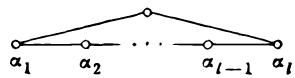
\includegraphics[keepaspectratio]{images/part002_112fabda.jpg}}

当 \(l = 1\) 时，仿射 Weyl 群的 Coxeter 图为

\pandocbounded{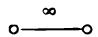
\includegraphics[keepaspectratio]{images/part002_c1e413d9.jpg}}

\begin{enumerate}
\def\labelenumi{(\Alph{enumi})}
\setcounter{enumi}{21}
\tightlist
\item
  \(R^{\prime} = R,\)
\end{enumerate}

\[
\Phi_ {\mathrm{R}} (x, y) = \frac {(x | y)}{2 (l + 1)}, \quad \gamma (\mathrm{R}) = (l + 1) ^ {2}.
\]

\begin{enumerate}
\def\labelenumi{(\Roman{enumi})}
\setcounter{enumi}{5}
\tightlist
\item
  基本权：
\end{enumerate}

\[
\begin{array}{l} \omega_ {i} = \varepsilon_ {1} + \dots + \varepsilon_ {i} - \frac {i}{l + 1} \sum_ {j = 1} ^ {l + 1} \varepsilon_ {j} \\ = \frac {1}{l + 1} [ (l - i + 1) (\alpha_ {1} + 2 \alpha_ {2} + \dots + (i - 1) \alpha_ {i - 1}) \\ \qquad + i ((l - i + 1) \alpha_ {i} + (l - i) \alpha_ {i + 1} + \dots + \alpha_ {l}) ]. \end{array}
\]

\begin{enumerate}
\def\labelenumi{(\Roman{enumi})}
\setcounter{enumi}{6}
\tightlist
\item
  正根之和：
\end{enumerate}

\[
\begin{array}{c} 2 \rho = l \varepsilon_ {1} + (l - 2) \varepsilon_ {2} + (l - 4) \varepsilon_ {3} + \dots - (l - 2) \varepsilon_ {l} - l \varepsilon_ {l + 1} \\ = l \alpha_ {1} + 2 (l - 1) \alpha_ {2} + \dots + i (l - i + 1) \alpha_ {i} + \dots + l \alpha_ {l}. \end{array}
\]

\begin{enumerate}
\def\labelenumi{(\Roman{enumi})}
\setcounter{enumi}{7}
\item
  Q(R)：坐标为整数且和为零的向量集。P(R)：由 Q(R) 与 \(\varepsilon_{1} - (l + 1)^{-1}(\varepsilon_{1} + \varepsilon_{2} + \cdots + \varepsilon_{l+1})\) 生成。P(R)/Q(R) 同构于 Z/(l+1)Z。连接指标：l + 1。
\item
  指数：1, 2, \ldots, l。
\item
  \(\mathrm{W}(\mathrm{R}) = \mathfrak{S}_{l + 1}\) ，可识别为 \(\varepsilon_{i}\) 的置换群。其阶为 \(\mathrm{W}(\mathrm{R})\colon (l + 1)!\)
\item
  \(l = 1\) : A(R) = W(R); \(w_0 = -1\) .
\end{enumerate}

\(l \geqslant 2: A(R) = W(R) \times \{1, -1\} \text{ 且 } w_{0} \text{ 将 } \alpha_{i} \text{ 变为 } -\alpha_{l+1-i}.\)

\begin{enumerate}
\def\labelenumi{(\Roman{enumi})}
\setcounter{enumi}{11}
\item
  群 \(\mathrm{P}(\mathrm{R}^{-})/\mathrm{Q}(\mathrm{R}^{-})\) 是阶为 \((l+1)\) 的循环群；它通过循环置换作用于扩展 Dynkin 图。当 \(l \geqslant 2\) 时，\(\mathrm{A}(\mathrm{R})/\mathrm{W}(\mathrm{R})\) 的唯一非恒等元作用于 \(\mathrm{P}(\mathrm{R})/\mathrm{Q}(\mathrm{R})\)，所用自同构为 \(x \mapsto -x\)。
\item
  Cartan 矩阵 \((l \times l)\) ：
\end{enumerate}

\[
\left( \begin{array}{c c c c c c c} 2 & - 1 & 0 & 0 & \dots & 0 & 0 \\ - 1 & 2 & - 1 & 0 & \dots & 0 & 0 \\ 0 & - 1 & 2 & - 1 & \dots & 0 & 0 \\ 0 & 0 & - 1 & 2 & \dots & 0 & 0 \\ \vdots & \vdots & \vdots & \vdots & \ddots & \vdots & \vdots \\ 0 & 0 & 0 & 0 & \dots & - 1 & 2 \end{array} \right)
\]

\specialchapter{\texorpdfstring{图版 II. \(B_{l}\) 型根系（\(l \geqslant 2\)）}{图版 II. B\_l 型根系 (l >= 2)}}

\begin{enumerate}
\def\labelenumi{(\Roman{enumi})}
\item
  \(V = E = R^{l}\) 。根：\(\pm\varepsilon_{i}, (1\leqslant i\leqslant l), \pm\varepsilon_{i}\pm\varepsilon_{j} (1\leqslant i<j\leqslant l).\) 根的数目：\(n = 2l^{2}\) 。
\item
  基：\(\alpha_{1} = \varepsilon_{1} - \varepsilon_{2},\alpha_{2} = \varepsilon_{2} - \varepsilon_{3},\ldots ,\alpha_{l - 1} = \varepsilon_{l - 1} - \varepsilon_{l},\alpha_{l} = \varepsilon_{l}\) 。正根：
\end{enumerate}

\[
\varepsilon_ {i} = \sum_ {i \leqslant k \leqslant l} \alpha_ {k} (1 \leqslant i \leqslant l),
\]

\[
\varepsilon_ {i} - \varepsilon_ {j} = \sum_ {i \leqslant k <   j} \alpha_ {k} (1 \leqslant i <   j \leqslant l),
\]

\[
\varepsilon_ {i} + \varepsilon_ {j} = \sum_ {i \leqslant k <   j} \alpha_ {k} + 2 \sum_ {j \leqslant k \leqslant l} \alpha_ {k} (1 \leqslant i <   j \leqslant l),
\]

\begin{enumerate}
\def\labelenumi{(\Roman{enumi})}
\setcounter{enumi}{2}
\item
  Coxeter 数：\(h = 2l\) 。
\item
  最高根：
\end{enumerate}

\[
\tilde {\alpha} = \varepsilon_ {1} + \varepsilon_ {2} = \alpha_ {1} + 2 \alpha_ {2} + 2 \alpha_ {3} + \dots + 2 \alpha_ {l}.
\]

有 \(\tilde{\alpha} = 2\omega_{2}\)，当 \(l = 2\) 时；有 \(\tilde{\alpha} = \omega_{2}\)，当 \(l \geqslant 3\) 时。

扩展 Dynkin 图：

当 \(l = 2\) 时：

\pandocbounded{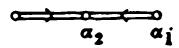
\includegraphics[keepaspectratio]{images/part002_ab2e3717.jpg}}

当 \(l\geqslant 3\) 时

\pandocbounded{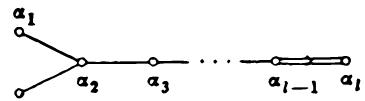
\includegraphics[keepaspectratio]{images/part002_677d35e2.jpg}}

\begin{enumerate}
\def\labelenumi{(\Alph{enumi})}
\setcounter{enumi}{21}
\tightlist
\item
  \(R^{\prime}\) 是向量集
\end{enumerate}

\[
\pm 2 \varepsilon_ {i} (1 \leqslant i \leqslant l), \pm \varepsilon_ {i} \pm \varepsilon_ {j} (1 \leqslant i <   j \leqslant l).
\]

\[
\Phi_ {\mathrm{R}} (x, y) = \frac {(x | y)}{4 l - 2}, \quad \gamma (\mathrm{R}) = (l + 1) (4 l - 2).
\]

\begin{enumerate}
\def\labelenumi{(\Roman{enumi})}
\setcounter{enumi}{5}
\tightlist
\item
  基本权：
\end{enumerate}

\[
\begin{array}{l} \omega_ {i} = \varepsilon_ {1} + \varepsilon_ {2} + \dots + \varepsilon_ {i} (1 \leqslant i <   l) \\ \quad = \alpha_ {1} + 2 \alpha_ {2} + \dots + (i - 1) \alpha_ {i - 1} + i (\alpha_ {i} + \alpha_ {i + 1} + \dots + \alpha_ {l}) \\ \omega_ {l} = \frac {1}{2} (\varepsilon_ {1} + \varepsilon_ {2} + \dots + \varepsilon_ {l}) \\ \quad = \frac {1}{2} (\alpha_ {1} + 2 \alpha_ {2} + \dots + l \alpha_ {l}). \end{array}
\]

\begin{enumerate}
\def\labelenumi{(\Roman{enumi})}
\setcounter{enumi}{6}
\tightlist
\item
  正根之和：
\end{enumerate}

\[
\begin{array}{l} 2 \rho = (2 l - 1) \varepsilon_ {1} + (2 l - 3) \varepsilon_ {2} + \dots + 3 \varepsilon_ {l - 1} + \varepsilon_ {l} \\ = (2 l - 1) \alpha_ {1} + 2 (2 l - 2) \alpha_ {2} + \dots + i (2 l - i) \alpha_ {i} + \dots + l ^ {2} \alpha_ {l}. \end{array}
\]

\begin{enumerate}
\def\labelenumi{(\Roman{enumi})}
\setcounter{enumi}{7}
\tightlist
\item
  \(\mathrm{Q}(\mathrm{R}) = \bigoplus_{i=1}^{l}\mathbf{Z}\varepsilon_i,\mathrm{P}(\mathrm{R}) = \bigoplus_{i=1}^{l}\mathbf{Z}\varepsilon_i + \mathbf{Z}(\frac{1}{2}\sum_{i=1}^{l}\varepsilon_i).\)
\end{enumerate}

\(P(R)/Q(R)\) 同构于 Z/2Z，由 \(\omega_{l}\) 的像生成。连接指标：2。

\begin{enumerate}
\def\labelenumi{(\Roman{enumi})}
\setcounter{enumi}{8}
\item
  指数：1, 3, 5, \ldots, 2l - 1。
\item
  W(R) 是群 \(S_{l}\)（通过对 \(\varepsilon_{i}\) 进行置换作用）与群 \((\mathbf{Z}/2\mathbf{Z})^{l}\)（通过 \(\varepsilon_{i} \mapsto (\pm1)_{i}\varepsilon_{i}\) 作用）的半直积。其阶为 \(2^{l}.l!\)
\item
  A(R) = W(R); \(w_{0} = -1\) .
\item
  \(P(R^{\prime})/Q(R^{\prime})\) 的唯一非平凡元确定扩展 Dynkin 图的唯一非平凡自同构。
\item
  Cartan 矩阵 \((l \times l)\) ：
\end{enumerate}

\[
\left( \begin{array}{c c c c c c c} 2 & - 1 & 0 & 0 & \dots & 0 & 0 \\ - 1 & 2 & - 1 & 0 & \dots & 0 & 0 \\ 0 & - 1 & 2 & - 1 & \dots & 0 & 0 \\ 0 & 0 & - 1 & 2 & \dots & 0 & 0 \\ \vdots & \vdots & \vdots & \vdots & \ddots & \vdots & \vdots \\ 0 & 0 & 0 & 0 & \dots & 2 & - 2 \\ 0 & 0 & 0 & 0 & \dots & - 1 & 2 \end{array} \right)
\]

\specialchapter{\texorpdfstring{图版 III. \(C_l\) 型根系（\(l \geqslant 2\)）}{图版 III. C\_l 型根系 (l >= 2)}}

\begin{enumerate}
\def\labelenumi{(\Roman{enumi})}
\item
  \(V = E = R^{l}.\) 根：\(\pm2\varepsilon_{i}\) 。 （ \(1\leqslant i\leqslant l\) ）。\(\pm\varepsilon_{i}\pm\varepsilon_{j}\)（ \(1\leqslant i<j\leqslant l\) ）。根的数目：\(n = 2l^{2}\) 。
\item
  基：\(\alpha_{1} = \varepsilon_{1} - \varepsilon_{2},\alpha_{2} = \varepsilon_{2} - \varepsilon_{3},\ldots ,\alpha_{l - 1} = \varepsilon_{l - 1} - \varepsilon_{l},\alpha_{l} = 2\varepsilon_{l}\) 。正根：
\end{enumerate}

\[
\varepsilon_ {i} - \varepsilon_ {j} = \sum_ {i \leqslant k <   j} \alpha_ {k} (1 \leqslant i <   j \leqslant l),
\]

\[
\varepsilon_ {i} + \varepsilon_ {j} = \sum_ {i \leqslant k <   j} \alpha_ {k} + 2 \sum_ {j \leqslant k <   l} \alpha_ {k} + \alpha_ {l} (1 \leqslant i <   j \leqslant l),
\]

\[
2 \varepsilon_ {i} = \sum_ {i \leqslant k <   l} \alpha_ {k} + \alpha_ {l} (1 \leqslant i \leqslant l).
\]

\begin{enumerate}
\def\labelenumi{(\Roman{enumi})}
\setcounter{enumi}{2}
\item
  Coxeter 数：\(h = 2l\) 。
\item
  最高根：
\end{enumerate}

\[
\tilde {\alpha} = 2 \varepsilon_ {1} = 2 \alpha_ {1} + 2 \alpha_ {2} + \dots + 2 \alpha_ {l - 1} + \alpha_ {l}.
\]

扩展 Dynkin 图：

\[
\alpha_ {1} \quad \alpha_ {2} \quad \dots \quad \alpha_ {l - 2} \quad \alpha_ {l - 1} \quad \alpha_ {l}
\]

\begin{enumerate}
\def\labelenumi{(\Alph{enumi})}
\setcounter{enumi}{21}
\tightlist
\item
  \(R^{\prime}\) 是向量集 \(\pm\varepsilon_{i}\) 。\(\pm\varepsilon_{i}\pm\varepsilon_{j}\) 。
\end{enumerate}

\[
\Phi_ {\mathrm{R}} (x, y) = \frac {(x | y)}{4 (l + 1)}, \quad \gamma (\mathrm{R}) = (l + 1) (4 l - 2).
\]

\begin{enumerate}
\def\labelenumi{(\Roman{enumi})}
\setcounter{enumi}{5}
\tightlist
\item
  基本权：
\end{enumerate}

\[
\begin{array}{r l} \omega_ {i} & = \varepsilon_ {1} + \varepsilon_ {2} + \dots + \varepsilon_ {i} (1 \leqslant i \leqslant l) \\ & = \alpha_ {1} + 2 \alpha_ {2} + \dots + (i - 1) \alpha_ {i - 1} \\ & \quad + i (\alpha_ {i} + \alpha_ {i + 1} + \dots + \alpha_ {l - 1} + \frac {1}{2} \alpha_ {l}). \end{array}
\]

\begin{enumerate}
\def\labelenumi{(\Roman{enumi})}
\setcounter{enumi}{6}
\tightlist
\item
  正根之和：
\end{enumerate}

\[
\begin{array}{r l} 2 \rho & = 2 l \varepsilon_ {1} + (2 l - 2) \varepsilon_ {2} + \dots + 4 \varepsilon_ {l - 1} + 2 \varepsilon_ {l} \\ & = 2 l \alpha_ {1} + 2 (2 l - 1) \alpha_ {2} + \dots + i (2 l - i + 1) \alpha_ {i} + \dots \\ & \qquad \dots + (l - 1) (l + 2) \alpha_ {l - 1} + \frac {1}{2} l (l + 1) \alpha_ {l}. \end{array}
\]

\begin{enumerate}
\def\labelenumi{(\Roman{enumi})}
\setcounter{enumi}{7}
\item
  Q(R)：坐标为整数且和为偶数的点集。\(P(R) = \bigoplus_{i=1}^{l} Z \varepsilon_i\) 。\(P(R)/Q(R)\) 同构于 \(Z/2Z\)，由 \(\omega_1\) 的像生成。\\
  连接指标：2。
\item
  指数：1, 3, 5, \ldots, 2l - 1。
\item
  W(R) 是群 \(S_{l}\)（通过对 \(\varepsilon_{i}\) 进行置换作用）与群 \((\mathbf{Z}/2\mathbf{Z})^{l}\)（通过 \(\varepsilon_{i} \mapsto (\pm1)_{i}\varepsilon_{i}\) 作用）的半直积。其阶为 \(2^{l}.l!\)
\item
  A(R) = W(R); \(w_{0} = -1\) .
\item
  \(P(R^{-})/Q(R^{-})\) 的唯一非平凡元确定扩展 Dynkin 图的唯一非平凡自同构。
\item
  Cartan 矩阵 \((l\times l)\) ：
\end{enumerate}

\[
\left( \begin{array}{c c c c c c c} 2 & - 1 & 0 & 0 & \dots & 0 & 0 \\ - 1 & 2 & - 1 & 0 & \dots & 0 & 0 \\ 0 & - 1 & 2 & - 1 & \dots & 0 & 0 \\ 0 & 0 & - 1 & 2 & \dots & 0 & 0 \\ \vdots & \vdots & \vdots & \vdots & \ddots & \vdots & \vdots \\ 0 & 0 & 0 & 0 & \dots & 2 & - 1 \\ 0 & 0 & 0 & 0 & \dots & - 2 & 2 \end{array} \right)
\]

\specialchapter{\texorpdfstring{图版 IV. \(D_{l}\) 型根系（\(l \geqslant 3\)）}{图版 IV. D\_l 型根系 (l >= 3)}}

\begin{enumerate}
\def\labelenumi{(\Roman{enumi})}
\tightlist
\item
  \(V = E = R^{l}\) 。根：\(\pm\varepsilon_{i}\pm\varepsilon_{j}(1\leqslant i<j\leqslant l)\)；（ \(\varepsilon_{i}\) ）是 \(R^{l}\) 的标准基。根的数目：\(n = 2l(l - 1)\) 。
\end{enumerate}

\begin{enumerate}
\def\labelenumi{(\Roman{enumi})}
\setcounter{enumi}{1}
\tightlist
\item
  基：\(\alpha_{1} = \varepsilon_{1} - \varepsilon_{2},\alpha_{2} = \varepsilon_{2} - \varepsilon_{3},\ldots ,\alpha_{l - 1} = \varepsilon_{l - 1} - \varepsilon_{l},\alpha_{l} = \varepsilon_{l - 1} + \varepsilon_{l}\) 。正根：
\end{enumerate}

\[
\varepsilon_ {i} - \varepsilon_ {j} = \sum_ {i <   k <   j} \alpha_ {k} (1 \leqslant i <   j \leqslant l).
\]

\[
\varepsilon_ {i} + \varepsilon_ {l} = \sum_ {i \leqslant k \leqslant l - 2} \alpha_ {k} + \alpha_ {l} (1 \leqslant i <   l),
\]

\[
\varepsilon_ {i} + \varepsilon_ {j} = \sum_ {i \leqslant k <   j} \alpha_ {k} + 2 \sum_ {j \leqslant k <   l - 1} \alpha_ {k} + \alpha_ {l - 1} + \alpha_ {l} (1 \leqslant i <   j <   l).
\]

\begin{enumerate}
\def\labelenumi{(\Roman{enumi})}
\setcounter{enumi}{2}
\item
  Coxeter 数：\(h = 2l - 2\) 。
\item
  最高根：
\end{enumerate}

\[
\tilde {\alpha} = \varepsilon_ {1} + \varepsilon_ {2} = \alpha_ {1} + 2 \alpha_ {2} + \dots + 2 \alpha_ {l - 2} + \alpha_ {l - 1} + \alpha_ {l}.
\]

有 \(\tilde{\alpha} = \omega_2 + \omega_3\)，当 \(l = 3\) 时；有 \(\tilde{\alpha} = \omega_2\)，当 \(l \geqslant 4\) 时。

扩展 Dynkin 图（l ≥ 4）：

\pandocbounded{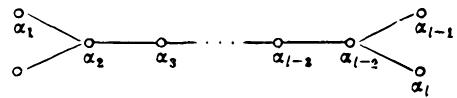
\includegraphics[keepaspectratio]{images/part002_b62b20f1.jpg}}

\begin{enumerate}
\def\labelenumi{(\Alph{enumi})}
\setcounter{enumi}{21}
\tightlist
\item
  \(R^{\prime} = R.\)
\end{enumerate}

\[
\Phi_ {R} (x, y) = \frac {(x | y)}{4 (l - 1)}, \quad \gamma (R) = 4 (l - 1) ^ {2}.
\]

\begin{enumerate}
\def\labelenumi{(\Roman{enumi})}
\setcounter{enumi}{5}
\tightlist
\item
  基本权：
\end{enumerate}

\[
\begin{array}{r l} \omega_ {i} & = \varepsilon_ {1} + \varepsilon_ {2} + \dots + \varepsilon_ {i} (1 \leqslant i \leqslant l - 2) \\ & = \alpha_ {1} + 2 \alpha_ {2} + \dots + (i - 1) \alpha_ {i - 1} + i (\alpha_ {i} + \alpha_ {i + 1} + \dots + \alpha_ {l - 2}) \\ & \quad + \frac {1}{2} i (\alpha_ {l - 1} + \alpha_ {l}) \\ \omega_ {l - 1} & = \frac {1}{2} (\varepsilon_ {1} + \varepsilon_ {2} + \dots + \varepsilon_ {l - 2} + \varepsilon_ {l - 1} - \varepsilon_ {l}) \\ & = \frac {1}{2} (\alpha_ {1} + 2 \alpha_ {2} + \dots + (l - 2) \alpha_ {l - 2} + \frac {1}{2} l \alpha_ {l - 1} + \frac {1}{2} (l - 2) \alpha_ {l}) \\ \omega_ {l} & = \frac {1}{2} (\varepsilon_ {1} + \varepsilon_ {2} + \dots + \varepsilon_ {l - 2} + \varepsilon_ {l - 1} + \varepsilon_ {l}) \\ & = \frac {1}{2} (\alpha_ {1} + 2 \alpha_ {2} + \dots + (l - 2) \alpha_ {l - 2} + \frac {1}{2} (l - 2) \alpha_ {l - 1} + \frac {1}{2} l \alpha_ {l}). \end{array}
\]

\begin{enumerate}
\def\labelenumi{(\Roman{enumi})}
\setcounter{enumi}{6}
\tightlist
\item
  正根之和：
\end{enumerate}

\[
\begin{array}{r l} 2 \rho & = 2 (l - 1) \varepsilon_ {1} + 2 (l - 2) \varepsilon_ {2} + \dots + 2 \varepsilon_ {l - 1} \\ & = 2 (l - 1) \alpha_ {1} + 2 (2 l - 3) \alpha_ {2} + \dots + 2 (i l - \frac {i (i + 1)}{2}) \alpha_ {i} + \dots \\ & \qquad \dots + \frac {l (l - 1)}{2} (\alpha_ {l - 1} + \alpha_ {l}). \end{array}
\]

\begin{enumerate}
\def\labelenumi{(\Roman{enumi})}
\setcounter{enumi}{7}
\tightlist
\item
  Q(R)：坐标为整数且和为偶数的点集。
\end{enumerate}

\[
\mathrm{P} (\mathrm{R}) = \bigoplus_ {i = 1} ^ {l} \mathbf {Z} \varepsilon_ {i} + \mathbf {Z} \left(\frac {1}{2} \sum_ {i = 1} ^ {l} \varepsilon_ {i}\right).
\]

l 为奇数时：\(\mathrm{P}(\mathrm{R})/\mathrm{Q}(\mathrm{R})\) 同构于 Z/4Z，由 \(\omega_{l}\) 的像生成；有 \(\omega_{1} \equiv 2\omega_{l}\) 和 \(\omega_{l-1} \equiv 3\omega_{l} \mod Q(\mathrm{R})\)。l 为偶数时：\(\mathrm{P}(\mathrm{R})/\mathrm{Q}(\mathrm{R})\) 同构于 \((\mathbf{Z}/2\mathbf{Z}) \times (\mathbf{Z}/2\mathbf{Z})\)；阶为 2 的三个元素是 \(\omega_{1}, \omega_{l-1}\) 和 \(\omega_{l}\) 的像。连接指标：4。

\begin{enumerate}
\def\labelenumi{(\Roman{enumi})}
\setcounter{enumi}{8}
\item
  指数：1, 3, 5, \ldots, 2l - 5, 2l - 3, l - 1（最后一个在 l 为偶数时出现两次，在 l 为奇数时出现一次）。
\item
  W(R) 是群 \(S_{l}\)（通过对 \(\varepsilon_{i}\) 进行置换作用）与群 \((\mathbf{Z}/2\mathbf{Z})^{l-1}\)（通过 \(\varepsilon_{i} \mapsto (\pm1)_{i}\varepsilon_{i}\) 作用，并满足 \(\prod_{i}(\pm1)_{i} = 1\)）的半直积。其阶为 \(2^{l-1}.l!\)
\item
  \(l \neq 4\)：A(R)/W(R) = Z/2Z 通过交换节点 \(\alpha_{l-1}\) 和 \(\alpha_l\) 作用于 Dynkin 图。\(l = 4\)：A(R)/W(R) = \(\mathfrak{S}_3\)，通过置换节点 \(\alpha_1, \alpha_3\) 和 \(\alpha_4\) 作用于 Dynkin 图。\(w_0 = -1\) 在 \(l\) 为偶数时成立；\(w_0 = -\varepsilon\) 在 \(l\) 为奇数时成立，其中 \(\varepsilon\) 是交换 \(\alpha_{l-1}\) 与 \(\alpha_l\) 并固定其余 \(\alpha_i\) 的自同构。
\item
  \(\mathrm{P}(\mathbb{R}^{-}) / \mathrm{Q}(\mathbb{R}^{-}) = \mathrm{P}(\mathbb{R}) / \mathrm{Q}(\mathbb{R})\) 在扩展 Dynkin 图上的作用：\(l\) 为奇数时，\(\omega_l\) 将 \(\alpha_0\) 变为 \(\alpha_1\)，将 \(\alpha_l\) 变为 \(\alpha_1\)，将 \(\alpha_1\) 变为 \(\alpha_{l-1}\)，并将 \(\alpha_{l-1}\) 变为 \(\alpha_0\)；它交换 \(\alpha_j\) 和 \(\alpha_{l-j}\)，其中 \(2 \leqslant j \leqslant l - 2\)。\(l\) 为偶数时，\(\omega_l\)（分别为 \(\omega_{l-1}\)）交换 \(\alpha_0\) 和 \(\alpha_l\)（分别为 \(\alpha_0\) 和 \(\alpha_{l-1}\)）、\(\alpha_1\) 和 \(\alpha_{l-1}\)（分别为 \(\alpha_1\) 和 \(\alpha_l\)），并交换 \(\alpha_j\) 和 \(\alpha_{l-j}\)，其中 \(2 \leqslant j \leqslant l - 2\)。
\end{enumerate}

\[
\left( \begin{array}{c c c c c c c} 2 & - 1 & \dots & 0 & 0 & 0 & 0 \\ - 1 & 2 & \dots & 0 & 0 & 0 & 0 \\ \vdots & \vdots & \ddots & \vdots & \vdots & \vdots & \vdots \\ 0 & 0 & \dots & 2 & - 1 & 0 & 0 \\ 0 & 0 & \dots & - 1 & 2 & - 1 & - 1 \\ 0 & 0 & \dots & 0 & - 1 & 2 & 0 \\ 0 & 0 & \dots & 0 & - 1 & 0 & 2 \end{array} \right)
\]

\begin{enumerate}
\def\labelenumi{(\Roman{enumi})}
\setcounter{enumi}{12}
\tightlist
\item
  Cartan 矩阵 \((l\times l)\) ：
\end{enumerate}

\specialchapter{\texorpdfstring{图版 V. \(E_{6}\) 型根系}{图版 V. E\_6 型根系}}

\begin{enumerate}
\def\labelenumi{(\Roman{enumi})}
\tightlist
\item
  V 是 \(E = R^{8}\) 的子空间，由坐标 \((\xi_{i})\) 满足 \(\xi_{6} = \xi_{7} = -\xi_{8}\) 的点组成。根：\(\pm\varepsilon_{i} \pm \varepsilon_{j} (1 \leqslant i < j \leqslant 5)\)，
\end{enumerate}

\[
\pm \frac {1}{2} (\varepsilon_ {8} - \varepsilon_ {7} - \varepsilon_ {6} + \sum_ {i = 1} ^ {5} (- 1) ^ {\nu (i)} \varepsilon_ {i}) \text {with} \sum_ {i = 1} ^ {5} \nu (i) \text {even.}
\]

根的数目：n = 72。

\begin{enumerate}
\def\labelenumi{(\Roman{enumi})}
\setcounter{enumi}{1}
\tightlist
\item
  基：\(\alpha_{1} = \frac{1}{2} (\varepsilon_{1} + \varepsilon_{8}) - \frac{1}{2} (\varepsilon_{2} + \varepsilon_{3} + \varepsilon_{4} + \varepsilon_{5} + \varepsilon_{6} + \varepsilon_{7}),\alpha_{2} = \varepsilon_{1} + \varepsilon_{2},\alpha_{3} =\) \(\varepsilon_2 - \varepsilon_1,\alpha_4 = \varepsilon_3 - \varepsilon_2,\alpha_5 = \varepsilon_4 - \varepsilon_3,\alpha_6 = \varepsilon_5 - \varepsilon_4.\) 正根：\(\pm \varepsilon_i + \varepsilon_j\) \(1\leqslant i <   j\leqslant 5)\)
\end{enumerate}

\[
\frac {1}{2} \left(\varepsilon_ {8} - \varepsilon_ {7} - \varepsilon_ {6} + \sum_ {i = 1} ^ {5} (- 1) ^ {\nu (i)} \varepsilon_ {i}\right) \text {with} \sum_ {i = 1} ^ {5} \nu (i) \text {even}.
\]

至少有一个系数 \(\geqslant 2\) 的正根（我们把根 \(a\alpha_{1} + b\alpha_{2} + c\alpha_{3} + d\alpha_{4} + e\alpha_{5} + f\alpha_{6}\) 记为 \({ }^{a c d e f}_{b})^{13}\)：

\[
\begin{array}{c c c c c c} 0   1   2   1   0 & 1   1   2   1   0 & 0   1   2   1   1 & 1   2   2   1   0 & 1   1   2   1   1 & 0   1   2   2   1 \\ 1 & 1 & 1 & 1 & 1 & 1 \\ 1   2   2   1   1 & 1   1   2   2   1 & 1   2   2   2   1 & 1   2   3   2   1 & 1   2   3   2   1 \\ 1 & 1 & 1 & 1 & 2 \end{array}
\]

\begin{enumerate}
\def\labelenumi{(\Roman{enumi})}
\setcounter{enumi}{2}
\item
  Coxeter 数：\(h = 12\) 。
\item
  最高根：
\end{enumerate}

\[
\begin{array}{r l} \tilde {\alpha} & = \frac {1}{2} (\varepsilon_ {1} + \varepsilon_ {2} + \varepsilon_ {3} + \varepsilon_ {4} + \varepsilon_ {5} - \varepsilon_ {6} - \varepsilon_ {7} + \varepsilon_ {8}) \\ & = \alpha_ {1} + 2 \alpha_ {2} + 2 \alpha_ {3} + 3 \alpha_ {4} + 2 \alpha_ {5} + \alpha_ {6} = \omega_ {2}. \end{array}
\]

扩展 Dynkin 图：

\pandocbounded{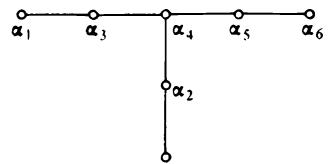
\includegraphics[keepaspectratio]{images/part002_985a73c0.jpg}}

\begin{enumerate}
\def\labelenumi{(\Alph{enumi})}
\setcounter{enumi}{21}
\tightlist
\item
  \(R^{\prime} = R.\)
\end{enumerate}

\[
  \Phi_ {\mathrm{R}} (x, y) = (x | y) / 24, \quad \gamma (\mathrm{R}) = 144.
\]

\begin{enumerate}
\def\labelenumi{(\Roman{enumi})}
\setcounter{enumi}{5}
\tightlist
\item
  基本权：
\end{enumerate}

\[
\begin{array}{l} \omega_ {1} = \frac {2}{3} (\varepsilon_ {8} - \varepsilon_ {7} - \varepsilon_ {6}) = \frac {1}{3} (4 \alpha_ {1} + 3 \alpha_ {2} + 5 \alpha_ {3} + 6 \alpha_ {4} + 4 \alpha_ {5} + 2 \alpha_ {6}) \\ \omega_ {2} = \frac {1}{2} (\varepsilon_ {1} + \varepsilon_ {2} + \varepsilon_ {3} + \varepsilon_ {4} + \varepsilon_ {5} - \varepsilon_ {6} - \varepsilon_ {7} + \varepsilon_ {8}) \\ \quad = \alpha_ {1} + 2 \alpha_ {2} + 2 \alpha_ {3} + 3 \alpha_ {4} + 2 \alpha_ {5} + \alpha_ {6} = \tilde {\alpha} \\ \omega_ {3} = \frac {5}{6} (\varepsilon_ {8} - \varepsilon_ {7} - \varepsilon_ {6}) + \frac {1}{2} (- \varepsilon_ {1} + \varepsilon_ {2} + \varepsilon_ {3} + \varepsilon_ {4} + \varepsilon_ {5}) \\ \quad = \frac {1}{3} (5 \alpha_ {1} + 6 \alpha_ {2} + 10 \alpha_ {3} + 12 \alpha_ {4} + 8 \alpha_ {5} + 4 \alpha_ {6}) \\ \omega_ {4} = \varepsilon_ {3} + \varepsilon_ {4} + \varepsilon_ {5} - \varepsilon_ {6} - \varepsilon_ {7} + \varepsilon_ {8} \\ \quad = 2 \alpha_ {1} + 3 \alpha_ {2} + 4 \alpha_ {3} + 6 \alpha_ {4} + 4 \alpha_ {5} + 2 \alpha_ {6} \\ \omega_ {5} = \frac {2}{3} (\varepsilon_ {8} - \varepsilon_ {7} - \varepsilon_ {6}) + \varepsilon_ {4} + \varepsilon_ {5} \\ \quad = \frac {1}{3} (4 \alpha_ {1} + 6 \alpha_ {2} + 8 \alpha_ {3} + 12 \alpha_ {4} + 10 \alpha_ {5} + 5 \alpha_ {6}) \\ \omega_ {6} = \frac {1}{3} (\varepsilon_ {8} - \varepsilon_ {7} - \varepsilon_ {6}) + \varepsilon_ {5} \\ \quad = \frac {1}{3} (2 \alpha_ {1} + 3 \alpha_ {2} + 4 \alpha_ {3} + 6 \alpha_ {4} + 5 \alpha_ {5} + 4 \alpha_ {6}). \end{array}
\]

\begin{enumerate}
\def\labelenumi{(\Roman{enumi})}
\setcounter{enumi}{6}
\tightlist
\item
  正根之和：
\end{enumerate}

\[
\begin{array}{l} 2 \rho = 2 (\varepsilon_ {2} + 2 \varepsilon_ {3} + 3 \varepsilon_ {4} + 4 \varepsilon_ {5} + 4 (\varepsilon_ {8} - \varepsilon_ {7} - \varepsilon_ {6})) \\ = 2 (8 \alpha_ {1} + 11 \alpha_ {2}) + 15 \alpha_ {3} + 21 \alpha_ {4} + 15 \alpha_ {5} + 8 \alpha_ {6}). \end{array}
\]

\begin{enumerate}
\def\labelenumi{(\Roman{enumi})}
\setcounter{enumi}{7}
\tightlist
\item
  P(R)/Q(R) 同构于 Z/3Z。
\end{enumerate}

连接指标：3。

\begin{enumerate}
\def\labelenumi{(\Roman{enumi})}
\setcounter{enumi}{8}
\item
  指数：1, 4, 5, 7, 8, 11。
\item
  W(R) 的阶：\(2^{7}.3^{4}.5\) 。
\item
  \(\mathrm{A}(\mathrm{R}) = \mathrm{W}(\mathrm{R}) \times \{1, -1\}\)；\(w_0\) 分别将 \(\alpha_1, \alpha_2, \alpha_3, \alpha_4, \alpha_5, \alpha_6\) 变为 \(-\alpha_6, -\alpha_2, -\alpha_5, -\alpha_4, -\alpha_3, -\alpha_1\)。
\item
  \(\mathrm{A}(\mathbb{R}) / \mathrm{W}(\mathbb{R})\) 的非恒等元确定自同构 \(x \mapsto -x\) 在 \(\mathrm{P}(\mathbb{R}) / \mathrm{Q}(\mathbb{R})\) 上的作用。
\end{enumerate}

扩展 Dynkin 图的自同构群同构于 \(S_{3}\)；其阶为 3 的元素由 \(P(R^{-})/Q(R^{-})\) 的两个非平凡元诱导。

\[
\left( \begin{array}{c c c c c c} 2 & 0 & - 1 & 0 & 0 & 0 \\ 0 & 2 & 0 & - 1 & 0 & 0 \\ - 1 & 0 & 2 & - 1 & 0 & 0 \\ 0 & - 1 & - 1 & 2 & - 1 & 0 \\ 0 & 0 & 0 & - 1 & 2 & - 1 \\ 0 & 0 & 0 & 0 & - 1 & 2 \end{array} \right)
\]

\begin{enumerate}
\def\labelenumi{(\Roman{enumi})}
\setcounter{enumi}{12}
\tightlist
\item
  Cartan 矩阵：
\end{enumerate}

\specialchapter{\texorpdfstring{图版 VI. \(E_{7}\) 型根系}{图版 VI. E\_7 型根系}}

\begin{enumerate}
\def\labelenumi{(\Roman{enumi})}
\tightlist
\item
  V 是 \(E = R^{8}\) 中正交于 \(\varepsilon_{7} + \varepsilon_{8}\) 的超平面。
\end{enumerate}

根：\(\pm \varepsilon_{i} \pm \varepsilon_{j} (1 \leqslant i < j \leqslant 6)\)，\(\pm (\varepsilon_{7} - \varepsilon_{8})\)，

\[
\pm \frac {1}{2} (\varepsilon_ {7} - \varepsilon_ {8} + \sum_ {i = 1} ^ {6} (- 1) ^ {\nu (i)} \varepsilon_ {i}) \quad \text { with } \sum_ {i = 1} ^ {8} \nu (i) \text { odd. }
\]

根的数目：n = 126。

\begin{enumerate}
\def\labelenumi{(\Roman{enumi})}
\setcounter{enumi}{1}
\tightlist
\item
  基：
\end{enumerate}

\[
\begin{array}{r l} \alpha_ {1} & = \frac {1}{2} (\varepsilon_ {1} + \varepsilon_ {8}) - \frac {1}{2} (\varepsilon_ {2} + \varepsilon_ {3} + \varepsilon_ {4} + \varepsilon_ {5} + \varepsilon_ {6} + \varepsilon_ {7}), \\ \alpha_ {2} & = \varepsilon_ {1} + \varepsilon_ {2}, \alpha_ {3} = \varepsilon_ {2} - \varepsilon_ {1}, \alpha_ {4} = \varepsilon_ {3} - \varepsilon_ {2}, \alpha_ {5} = \varepsilon_ {4} - \varepsilon_ {3}, \\ \alpha_ {6} & = \varepsilon_ {5} - \varepsilon_ {4}, \alpha_ {7} = \varepsilon_ {6} - \varepsilon_ {5}. \end{array}
\]

正根：

\[
\begin{array}{c} \pm \varepsilon_ {i} + \varepsilon_ {j} (1 \leqslant i <   j \leqslant 6), - \varepsilon_ {7} + \varepsilon_ {8}, \\ \frac {1}{2} (- \varepsilon_ {7} + \varepsilon_ {8} + \sum_ {i = 1} ^ {6} (- 1) ^ {\nu (i)} \varepsilon_ {i}) \quad \text { with } \sum_ {i = 1} ^ {6} \nu (i) \text { odd }. \end{array}
\]

含有 \(\alpha_{7}\) 且至少有一个系数 \(\geqslant 2\) 的正根（我们把根 \(a\alpha_{1} + b\alpha_{2} + c\alpha_{3} + d\alpha_{4} + e\alpha_{5} + f\alpha_{6} + g\alpha_{7}\) 记为 \(\frac{a c d e f g}{b})^{14}\)：

\[
\begin{array}{c c c c c} 0   1   2   1   1   1 & 1   1   2   1   1   1 & 0   1   2   2   1   1 & 1   2   2   1   1   1 & 1   1   2   2   1   1 \\ 1 & 1 & 1 & 1 & 1 \\ 0   1   2   2   2   1 & 1   2   2   2   1   1 & 1   1   2   2   2   1 & 1   2   2   2   2   1 & 1   2   3   2   1   1 \\ 1 & 1 & 1 & 1 & 1 \\ 1   2   3   2   2   1 & 1   2   3   2   1   1 & 1   2   3   3   2   1 & 1   2   3   2   2   1 & 1   2   3   3   2   1 \\ 1 & 2 & 1 & 2 & 2 \end{array}
\]

\[
\begin{array}{c c c} 1 2 4 3 2 1 & 1 3 4 3 2 1 & 2 3 4 3 2 1 \\ 2 & 2 & 2 \end{array}
\]

\begin{enumerate}
\def\labelenumi{(\Roman{enumi})}
\setcounter{enumi}{2}
\item
  Coxeter 数：\(h = 18\) 。
\item
  最高根：
\end{enumerate}

\[
\tilde {\alpha} = \varepsilon_ {8} - \varepsilon_ {7} = 2 \alpha_ {1} + 2 \alpha_ {2} + 3 \alpha_ {3} + 4 \alpha_ {4} + 3 \alpha_ {5} + 2 \alpha_ {6} + \alpha_ {7} = \omega_ {1}.
\]

扩展 Dynkin 图：

\[
\alpha_ {1} \quad \alpha_ {3} \quad \alpha_ {4} \quad \alpha_ {5} \quad \alpha_ {6} \quad \alpha_ {7}
\]

\begin{enumerate}
\def\labelenumi{(\Alph{enumi})}
\setcounter{enumi}{21}
\tightlist
\item
  \(R^{\prime} = R.\)
\end{enumerate}

\[
  \Phi_ {\mathrm{R}} (x, y) = (x | y) / 36, \quad \gamma (\mathrm{R}) = 2 ^ {2}. 3 ^ {4}.
\]

\begin{enumerate}
\def\labelenumi{(\Roman{enumi})}
\setcounter{enumi}{5}
\tightlist
\item
  基本权：
\end{enumerate}

\[
\begin{array}{l} \omega_ {1} = \varepsilon_ {8} - \varepsilon_ {7} = 2 \alpha_ {1} + 2 \alpha_ {2} + 3 \alpha_ {3} + 4 \alpha_ {4} + 3 \alpha_ {5} + 2 \alpha_ {6} + \alpha_ {7} \\ \omega_ {2} = \frac {1}{2} (\varepsilon_ {1} + \varepsilon_ {2} + \varepsilon_ {3} + \varepsilon_ {4} + \varepsilon_ {5} + \varepsilon_ {6} - 2 \varepsilon_ {7} + 2 \varepsilon_ {8}) \\ \qquad = \frac {1}{2} (4 \alpha_ {1} + 7 \alpha_ {2} + 8 \alpha_ {3} + 12 \alpha_ {4} + 9 \alpha_ {5} + 8 \alpha_ {6} + 3 \alpha_ {7}) \\ \omega_ {3} = \frac {1}{2} (- \varepsilon_ {1} + \varepsilon_ {2} + \varepsilon_ {3} + \varepsilon_ {4} + \varepsilon_ {5} + \varepsilon_ {6} - 3 \varepsilon_ {7} + 3 \varepsilon_ {8}) \\ \qquad = 3 \alpha_ {1} + 4 \alpha_ {2} + 6 \alpha_ {3} + 8 \alpha_ {4} + 6 \alpha_ {5} + 4 \alpha_ {6} + 2 \alpha_ {7} \\ \omega_ {4} = \varepsilon_ {3} + \varepsilon_ {4} + \varepsilon_ {5} + \varepsilon_ {6} + 2 (\varepsilon_ {8} - \varepsilon_ {7}) \\ \qquad = 4 \alpha_ {1} + 6 \alpha_ {2} + 8 \alpha_ {3} + 12 \alpha_ {4} + 9 \alpha_ {5} + 6 \alpha_ {6} + 3 \alpha_ {7} \\ \omega_ {5} = \varepsilon_ {4} + \varepsilon_ {5} + \varepsilon_ {6} + \frac {3}{2} (\varepsilon_ {8} - \varepsilon_ {7}) \\ \qquad = \frac {1}{2} (6 \alpha_ {1} + 9 \alpha_ {2} + 12 \alpha_ {3} + 18 \alpha_ {4} + 15 \alpha_ {5} + 10 \alpha_ {6} + 5 \alpha_ {7}) \\ \omega_ {6} = \varepsilon_ {5} + \varepsilon_ {6} - \varepsilon_ {7} + \varepsilon_ {8} \\ \qquad = 2 \alpha_ {1} + 3 \alpha_ {2} + 4 \alpha_ {3} + 6 \alpha_ {4} + 5 \alpha_ {5} + 4 \alpha_ {6} + 2 \alpha_ {7} \\ \omega_ {7} = \varepsilon_ {6} + \frac {1}{2} (\varepsilon_ {8} - \varepsilon_ {7}) \\ \qquad = \frac {1}{2} (2 \alpha_ {1} + 3 \alpha_ {2} + 4 \alpha_ {3} + 6 \alpha_ {4} + 5 \alpha_ {5} + 4 \alpha_ {6} + 3 \alpha_ {7}). \end{array}
\]

\begin{enumerate}
\def\labelenumi{(\Roman{enumi})}
\setcounter{enumi}{6}
\tightlist
\item
  正根之和：
\end{enumerate}

\[
\begin{array}{l} 2 \rho = 2 \varepsilon_ {2} + 4 \varepsilon_ {3} + 6 \varepsilon_ {4} + 8 \varepsilon_ {5} + 10 \varepsilon_ {6} - 17 \varepsilon_ {7} + 17 \varepsilon_ {8} \\ = 34 \alpha_ {1} + 49 \alpha_ {2} + 66 \alpha_ {3} + 96 \alpha_ {4} + 75 \alpha_ {5} + 52 \alpha_ {6} + 27 \alpha_ {7}. \end{array}
\]


\begin{enumerate}
\def\labelenumi{(\Roman{enumi})}
\setcounter{enumi}{7}
\item
  P(R)/Q(R) 同构于 Z/2Z。连接指标：2。
\item
  指数：1, 5, 7, 9, 11, 13, 17。
\item
  W(R) 的阶：\(2^{10}.3^{4}.5.7\) 。
\item
  A(R) = W(R), \(w_{0} = -1\) .
\item
  \(P(R^{\prime})/Q(R^{\prime})\) 只有一个非恒等元：它确定 Dynkin 图的唯一非平凡自同构。
\end{enumerate}

\[
\left( \begin{array}{c c c c c c c} 2 & 0 & - 1 & 0 & 0 & 0 & 0 \\ 0 & 2 & 0 & - 1 & 0 & 0 & 0 \\ - 1 & 0 & 2 & - 1 & 0 & 0 & 0 \\ 0 & - 1 & - 1 & 2 & - 1 & 0 & 0 \\ 0 & 0 & 0 & - 1 & 2 & - 1 & 0 \\ 0 & 0 & 0 & 0 & - 1 & 2 & - 1 \\ 0 & 0 & 0 & 0 & 0 & - 1 & 2 \end{array} \right)
\]

\begin{enumerate}
\def\labelenumi{(\Roman{enumi})}
\setcounter{enumi}{12}
\tightlist
\item
  Cartan 矩阵：
\end{enumerate}

\specialchapter{\texorpdfstring{图版 VII. \(\mathbf{E}_8\) 型根系}{图版 VII. E\_8 型根系}}

\begin{enumerate}
\def\labelenumi{(\Roman{enumi})}
\tightlist
\item
  \(V = E = R^{8}.\)
\end{enumerate}

\[
\begin{array}{l} \text {Roots:} \pm \varepsilon_ {i} \pm \varepsilon_ {j} (i <   j), \frac {1}{2} \sum_ {i = 1} ^ {8} (- 1) ^ {\nu (\mathrm{i})} \varepsilon_ {i} \text {with} \sum_ {i = 1} ^ {8} \nu (i) \text {even.} \\ \text {Number of roots:} n = 240. \end{array}
\]

\begin{enumerate}
\def\labelenumi{(\Roman{enumi})}
\setcounter{enumi}{1}
\tightlist
\item
  基：
\end{enumerate}

\[
\begin{array}{r l} \alpha_ {1} & = \frac {1}{2} (\varepsilon_ {1} + \varepsilon_ {8}) - \frac {1}{2} (\varepsilon_ {2} + \varepsilon_ {3} + \varepsilon_ {4} + \varepsilon_ {5} + \varepsilon_ {6} + \varepsilon_ {7}), \\ \alpha_ {2} & = \varepsilon_ {1} + \varepsilon_ {2}, \alpha_ {3} = \varepsilon_ {2} - \varepsilon_ {1}, \alpha_ {4} = \varepsilon_ {3} - \varepsilon_ {2}, \alpha_ {5} = \varepsilon_ {4} - \varepsilon_ {3}, \\ \alpha_ {6} & = \varepsilon_ {5} - \varepsilon_ {4}, \alpha_ {7} = \varepsilon_ {6} - \varepsilon_ {5}, \alpha_ {8} = \varepsilon_ {7} - \varepsilon_ {6}. \end{array}
\]

正根：

\[
\pm \varepsilon_ {i} + \varepsilon_ {j} (i <   j), \frac {1}{2} (\varepsilon_ {8} + \sum_ {i = 1} ^ {7} (- 1) ^ {\nu (\mathrm{i})} \varepsilon_ {i}) \text {with} \sum_ {i = 1} ^ {7} \nu (i) \text {even}.
\]

含有 \(\alpha_{8}\) 且至少有一个系数 \(\geqslant 2\) 的正根（我们把根 \(a\alpha_{1} + b\alpha_{2} + c\alpha_{3} + d\alpha_{4} + e\alpha_{5} + f\alpha_{6} + g\alpha_{7} + h\alpha_{8}\) 记为 \(\left.\frac{a}{b}c\frac{d}{e}\frac{e}{f}\frac{g}{h}\right)^{15}\)：

\[
\begin{array}{c c c c c} 0   1   2   1   1   1   1 & 0   1   2   2   1   1   1 & 1   1   2   1   1   1   1 & 0   1   2   2   2   1   1 & 1   2   2   1   1   1   1 \\ 1 & 1 & 1 & 1 & 1 \\ 1   1   2   2   1   1   1 & 1   2   2   2   1   1   1 & 1   1   2   2   2   1   1 & 0   1   2   2   2   2   1 & 1   2   3   2   1   1   1 \\ 1 & 1 & 1 & 1 & 1 \\ 1   2   2   2   2   1   1 & 1   1   2   2   2   2   1 & 1   2   3   2   2   1   1 & 1   2   3   2   2   1   1 & 1   2   2   2   2   2   1 \\ 1 & 1 & 2 & 1 & 1 \\ 1   2   3   2   2   1   1 & 1   2   3   3   2   1   1 & 1   2   3   2   2   2   1 & 1   2   3   3   2   1   1 & 1   2   3   2   2   2   1 \\ 2 & 1 & 1 & 2 & 2 \end{array}
\]

\[
\begin{array}{c c c c c} 1   2   3   3   3   2   1 & 1   2   4   3   2   1   1 & 1   2   3   3   2   2   1 & 1   2   3   3   3   2   1 & 1   3   4   3   2   1   1 \\ 1 & 2 & 2 & 1 & 2 \\ 1   2   4   3   2   2   1 & 1   2   3   3   3   2   1 & 2   3   4   3   2   1   1 & 1   3   4   3   2   2   1 & 1   2   4   3   3   2   1 \\ 2 & 2 & 2 & 2 & 2 \\ 2   3   4   3   2   2   1 & 1   3   4   3   3   2   1 & 1   2   4   4   3   2   1 & 2   3   4   3   3   2   1 & 1   3   4   4   3   2   1 \\ 2 & 2 & 2 & 2 & 2 \\ 1   3   5   4   3   2   1 & 2   3   4   4   3   2   1 & 1   3   5   4   3   2   1 & 2   3   5   4   3   2   1 & 2   3   5   4   3   2   1 \\ 2 & 2 & 3 & 2 & 3 \\ \text { } _ {2} ^ {2} \text { } _ {5} ^ {4} \text { } _ {5} ^ {4} \text { } _ {5} ^ {4} \text { } _ {5} ^ {4} \text { } _ {5} ^ {4} \text { } _ {5} ^ {4} \text { } _ {5} ^ {4} \text { } _ {5} ^ {4} \text { } _ {5} ^ {4} \text {(} _ {2} ^ {2} \text {)} _ {2} ^ {3} \text {)} _ {3} ^ {3} \text {)} _ {3} ^ {3} \text {)} _ {3} ^ {3} \end{array}
\]

\begin{enumerate}
\def\labelenumi{(\Roman{enumi})}
\setcounter{enumi}{2}
\item
  Coxeter 数：\(h = 30\) 。
\item
  最高根：
\end{enumerate}

\[
\begin{array}{r l} \tilde {\alpha} & = \varepsilon_ {7} + \varepsilon_ {8} = 2 \alpha_ {1} + 3 \alpha_ {2} + 4 \alpha_ {3} + 6 \alpha_ {4} + 5 \alpha_ {5} + 4 \alpha_ {6} + 3 \alpha_ {7} + 2 \alpha_ {8} \\ & = \omega_ {8}. \end{array}
\]

扩展 Dynkin 图为：

\[
\begin{array}{c} \alpha_ {1} \quad \alpha_ {3} \\ \alpha_ {4} \quad \alpha_ {5} \quad \alpha_ {6} \quad \alpha_ {7} \quad \alpha_ {8} \\ \alpha_ {2} \end{array}
\]

\begin{enumerate}
\def\labelenumi{(\Alph{enumi})}
\setcounter{enumi}{21}
\tightlist
\item
  \(R^{\prime} = R.\)
\end{enumerate}

\[
  \Phi_ {\mathrm{R}} (x, y) = (x | y) / 60, \quad \gamma (\mathrm{R}) = 900.
\]

\begin{enumerate}
\def\labelenumi{(\Roman{enumi})}
\setcounter{enumi}{5}
\tightlist
\item
  基本权：
\end{enumerate}

\[
\begin{array}{l} \omega_ {1} = 2 \varepsilon_ {8} = 4 \alpha_ {1} + 5 \alpha_ {2} + 7 \alpha_ {3} + 10 \alpha_ {4} + 8 \alpha_ {5} + 6 \alpha_ {6} + 4 \alpha_ {7} + 2 \alpha_ {8} \\ \omega_ {2} = \frac {1}{2} (\varepsilon_ {1} + \varepsilon_ {2} + \varepsilon_ {3} + \varepsilon_ {4} + \varepsilon_ {5} + \varepsilon_ {6} + \varepsilon_ {7} + 5 \varepsilon_ {8}) \\ \quad = 5 \alpha_ {1} + 8 \alpha_ {2} + 10 \alpha_ {3} + 15 \alpha_ {4} + 12 \alpha_ {5} + 9 \alpha_ {6} + 6 \alpha_ {7} + 3 \alpha_ {8} \\ \omega_ {3} = \frac {1}{2} (- \varepsilon_ {1} + \varepsilon_ {2} + \varepsilon_ {3} + \varepsilon_ {4} + \varepsilon_ {5} + \varepsilon_ {6} + \varepsilon_ {7} + 7 \varepsilon_ {8}) \\ \quad = 7 \alpha_ {1} + 10 \alpha_ {2} + 14 \alpha_ {3} + 20 \alpha_ {4} + 16 \alpha_ {5} + 12 \alpha_ {6} + 8 \alpha_ {7} + 4 \alpha_ {8} \\ \omega_ {4} = \varepsilon_ {3} + \varepsilon_ {4} + \varepsilon_ {5} + \varepsilon_ {6} + \varepsilon_ {7} + 5 \varepsilon_ {8} \\ \quad = 10 \alpha_ {1} + 15 \alpha_ {2} + 20 \alpha_ {3} + 30 \alpha_ {4} + 24 \alpha_ {5} + 18 \alpha_ {6} + 12 \alpha_ {7} + 6 \alpha_ {8} \end{array}
\]

\[
\begin{array}{r l} \omega_ {5} & = \varepsilon_ {4} + \varepsilon_ {5} + \varepsilon_ {6} + \varepsilon_ {7} + 4 \varepsilon_ {8} \\ & = 8 \alpha_ {1} + 12 \alpha_ {2} + 16 \alpha_ {3} + 24 \alpha_ {4} + 20 \alpha_ {5} + 15 \alpha_ {6} + 10 \alpha_ {7} + 5 \alpha_ {8} \\ \omega_ {6} & = \varepsilon_ {5} + \varepsilon_ {6} + \varepsilon_ {7} + 3 \varepsilon_ {8} \\ & = 6 \alpha_ {1} + 9 \alpha_ {2} + 12 \alpha_ {3} + 18 \alpha_ {4} + 15 \alpha_ {5} + 12 \alpha_ {6} + 8 \alpha_ {7} + 4 \alpha_ {8} \\ \omega_ {7} & = \varepsilon_ {6} + \varepsilon_ {7} + 2 \varepsilon_ {8} \\ & = 4 \alpha_ {1} + 6 \alpha_ {2} + 8 \alpha_ {3} + 12 \alpha_ {4} + 10 \alpha_ {5} + 8 \alpha_ {6} + 6 \alpha_ {7} + 3 \alpha_ {8} \\ \omega_ {8} & = \varepsilon_ {7} + \varepsilon_ {8} \\ & = 5 \alpha_ {1} + 8 \alpha_ {2} + 10 \alpha_ {3} + 15 \alpha_ {4} + 12 \alpha_ {5} + 9 \alpha_ {6} + 6 \alpha_ {7} + 3 \alpha_ {8} = \tilde {\alpha}. \end{array}
\]

\begin{enumerate}
\def\labelenumi{(\Roman{enumi})}
\setcounter{enumi}{6}
\tightlist
\item
  正根之和：
\end{enumerate}

\[
\begin{array}{r l} 2 \rho & = 2 (\varepsilon_ {2} + 2 \varepsilon_ {3} + 3 \varepsilon_ {4} + 4 \varepsilon_ {5} + 5 \varepsilon_ {6} + 6 \varepsilon_ {7} + 23 \varepsilon_ {8}) \\ & = 2 (46 \alpha_ {1} + 68 \alpha_ {2} + 91 \alpha_ {3} + 135 \alpha_ {4} + 110 \alpha_ {5} + 84 \alpha_ {6} + 57 \alpha_ {7} + 29 \alpha_ {8}). \end{array}
\]

\begin{enumerate}
\def\labelenumi{(\Roman{enumi})}
\setcounter{enumi}{7}
\tightlist
\item
  Q(R)：坐标为 \(\xi_{i}\) 且满足 \(2\xi_{i} \in \mathbf{Z}\) 的点集，
\end{enumerate}

\[
\begin{array}{l} \xi_ {i} - \xi_ {j} \in \mathbf {Z}, \sum_ {i = 1} ^ {8} \xi_ {i} \in 2 \mathbf {Z}. \\ \text { Connection   index: } 1. \end{array}
\]

\begin{enumerate}
\def\labelenumi{(\Roman{enumi})}
\setcounter{enumi}{8}
\item
  指数：1, 7, 11, 13, 17, 19, 23, 29。
\item
  W(R) 的阶：\(2^{14}.3^{5}.5^{2}.7\) 。
\item
  以及（XII）\(A(R) = W(R). w_0 = -1.\)
\item
  Cartan 矩阵：
\end{enumerate}

\[
\left( \begin{array}{c c c c c c c c} 2 & 0 & - 1 & 0 & 0 & 0 & 0 & 0 \\ 0 & 2 & 0 & - 1 & 0 & 0 & 0 & 0 \\ - 1 & 0 & 2 & - 1 & 0 & 0 & 0 & 0 \\ 0 & - 1 & - 1 & 2 & - 1 & 0 & 0 & 0 \\ 0 & 0 & 0 & - 1 & 2 & - 1 & 0 & 0 \\ 0 & 0 & 0 & 0 & - 1 & 2 & - 1 & 0 \\ 0 & 0 & 0 & 0 & 0 & - 1 & 2 & - 1 \\ 0 & 0 & 0 & 0 & 0 & 0 & - 1 & 2 \end{array} \right)
\]

\specialchapter{\texorpdfstring{图版 VIII. \(F_{4}\) 型根系}{图版 VIII. F\_4 型根系}}

\begin{enumerate}
\def\labelenumi{(\Roman{enumi})}
\tightlist
\item
  \(V = E = R^4.\)
\end{enumerate}

根：

\[
\begin{array}{c} \pm \varepsilon_ {i}. (1 \leqslant i \leqslant 4), \quad \pm \varepsilon_ {i} \pm \varepsilon_ {j} (1 \leqslant i <   j \leqslant 4), \\ \frac {1}{2} (\pm \varepsilon_ {1} \pm \varepsilon_ {2} \pm \varepsilon_ {3} \pm \varepsilon_ {4}). \end{array}
\]

根的数目：n = 48。

\begin{enumerate}
\def\labelenumi{(\Roman{enumi})}
\setcounter{enumi}{1}
\tightlist
\item
  基：
\end{enumerate}

\[
\alpha_ {1} = \varepsilon_ {2} - \varepsilon_ {3}, \alpha_ {2} = \varepsilon_ {3} - \varepsilon_ {4}, \alpha_ {3} = \varepsilon_ {4}, \alpha_ {4} = \frac {1}{2} (\varepsilon_ {1} - \varepsilon_ {2} - \varepsilon_ {3} - \varepsilon_ {4}).
\]

正根：

\[
\varepsilon_ {i} (1 \leqslant i \leqslant 4), \quad \varepsilon_ {i} \pm \varepsilon_ {j} (1 \leqslant i <   j \leqslant 4). \quad \frac {1}{2} (\varepsilon_ {1} \pm \varepsilon_ {2} \pm \varepsilon_ {3} \pm \varepsilon_ {4}).
\]

至少有一个系数 \(\geqslant2\) 的正根（我们把根 \(a\alpha_{1}+b\alpha_{2}+c\alpha_{3}+d\alpha_{4}\) 记为 abcd）\(^{16}\)：

\[
\begin{array}{c c c c c c c c} 0 1 2 0 & 1 1 2 0 & 0 1 2 1 & 1 2 2 0 & 1 1 2 1 & 0 1 2 2 & 1 2 2 1 & 1 1 2 2 \\ & 1 2 3 1 & 1 2 2 2 & 1 2 3 2 & 1 2 4 2 & 1 3 4 2 & 2 3 4 2 \end{array}
\]

\begin{enumerate}
\def\labelenumi{(\Roman{enumi})}
\setcounter{enumi}{2}
\item
  根的数目：\(h = 12\) 。
\item
  最高根：\(\tilde{\alpha} = \varepsilon_1 + \varepsilon_2 = 2\alpha_1 + 3\alpha_2 + 4\alpha_3 + 2\alpha_4 = \omega_1\) 。扩展 Dynkin 图：
\end{enumerate}

\pandocbounded{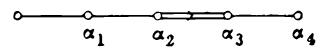
\includegraphics[keepaspectratio]{images/part002_560ef793.jpg}}

\begin{enumerate}
\def\labelenumi{(\Alph{enumi})}
\setcounter{enumi}{21}
\tightlist
\item
  \(R^{\prime}\) 是向量集 \(\pm2\varepsilon_{i},\pm\varepsilon_{i}\pm\varepsilon_{j},\pm\varepsilon_{1}\pm\varepsilon_{2}\pm\varepsilon_{3}\pm\varepsilon_{4}.\)
\end{enumerate}

\[
  \Phi_ {\mathrm{R}} (x, y) = \frac {(x | y)}{18}, \quad \gamma (\mathrm{R}) = 2. 3 ^ {4}.
\]

\begin{enumerate}
\def\labelenumi{(\Roman{enumi})}
\setcounter{enumi}{5}
\tightlist
\item
  基本权：
\end{enumerate}

\[
\omega_ {1} = \varepsilon_ {1} + \varepsilon_ {2} = 2 \alpha_ {1} + 3 \alpha_ {2} + 4 \alpha_ {3} + 2 \alpha_ {4}
\]

\[
\omega_ {2} = 2 \varepsilon_ {1} + \varepsilon_ {2} + \varepsilon_ {3} = 3 \alpha_ {1} + 6 \alpha_ {2} + 8 \alpha_ {3} + 4 \alpha_ {4}
\]

\[
\omega_ {3} = \frac {1}{2} (3 \varepsilon_ {1} + \varepsilon_ {2} + \varepsilon_ {3} + \varepsilon_ {4}) = 2 \alpha_ {1} + 4 \alpha_ {2} + 6 \alpha_ {3} + 3 \alpha_ {4}
\]

\[
\omega_ {4} = \varepsilon_ {1} = \alpha_ {1} + 2 \alpha_ {2} + 3 \alpha_ {3} + 2 \alpha_ {4}.
\]

\begin{enumerate}
\def\labelenumi{(\Roman{enumi})}
\setcounter{enumi}{6}
\tightlist
\item
  正根之和：
\end{enumerate}

\[
2 \rho = 11 \varepsilon_ {1} + 5 \varepsilon_ {2} + 3 \varepsilon_ {3} + \varepsilon_ {4} = 16 \alpha_ {1} + 30 \alpha_ {2} + 42 \alpha_ {3} + 22 \alpha_ {4}.
\]

\begin{enumerate}
\def\labelenumi{(\Roman{enumi})}
\setcounter{enumi}{7}
\tightlist
\item
  \(\mathrm{Q}(\mathrm{R}) = \bigoplus_{i=1}^{4} \mathbf{Z} \varepsilon_i + \mathbf{Z}\left(\frac{1}{2} \sum_{i=1}^{4} \varepsilon_i\right)\) .
\end{enumerate}

\(P(R) = Q(R).\)

连接指标：1。

\begin{enumerate}
\def\labelenumi{(\Roman{enumi})}
\setcounter{enumi}{8}
\item
  指数：1, 5, 7, 11。
\item
  以及（XI）A(R) = W(R)，\(w_{0} = -1\) 。
\item
  Cartan 矩阵：
\end{enumerate}

\[
\left( \begin{array}{c c c c} 2 & - 1 & 0 & 0 \\ - 1 & 2 & - 2 & 0 \\ 0 & - 1 & 2 & - 1 \\ 0 & 0 & - 1 & 2 \end{array} \right)
\]

\specialchapter{\texorpdfstring{图版 IX. \(\mathbf{G}_2\) 型根系}{图版 IX. G\_2 型根系}}

\begin{enumerate}
\def\labelenumi{(\Roman{enumi})}
\tightlist
\item
  V 是 \(E = R^{3}\) 中方程为 \(\xi_{1} + \xi_{2} + \xi_{3} = 0\) 的超平面。根：
\end{enumerate}

\[
\begin{array}{c} \pm (\varepsilon_ {1} - \varepsilon_ {2}), \quad \pm (\varepsilon_ {1} - \varepsilon_ {3}), \quad \pm (\varepsilon_ {2} - \varepsilon_ {3}), \quad \pm (2 \varepsilon_ {1} - \varepsilon_ {2} - \varepsilon_ {3}), \\ \pm (2 \varepsilon_ {2} - \varepsilon_ {1} - \varepsilon_ {3}), \quad \pm (2 \varepsilon_ {3} - \varepsilon_ {1} - \varepsilon_ {2}). \end{array}
\]

根的数目：n = 12。

\begin{enumerate}
\def\labelenumi{(\Roman{enumi})}
\setcounter{enumi}{1}
\item
  基：\(\alpha_{1} = \varepsilon_{1} - \varepsilon_{2},\alpha_{2} = -2\varepsilon_{1} + \varepsilon_{2} + \varepsilon_{3}\) 。正根：\(\alpha_{1},\alpha_{1} + \alpha_{2},2\alpha_{1} + \alpha_{2},3\alpha_{1} + \alpha_{2},3\alpha_{1} + 2\alpha_{2}\) 。
\item
  Coxeter 数：h = 6。
\item
  最高根：\(\tilde{\alpha} = -\varepsilon_1 - \varepsilon_2 + 2\varepsilon_3 = 3\alpha_1 + 2\alpha_2 = \omega_2\) 。扩展 Dynkin 图：
\end{enumerate}

\pandocbounded{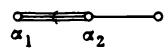
\includegraphics[keepaspectratio]{images/part002_d2921928.jpg}}

\begin{enumerate}
\def\labelenumi{(\Alph{enumi})}
\setcounter{enumi}{21}
\tightlist
\item
  \(R^{\prime}\) 是向量集
\end{enumerate}

\[
\pm \alpha_ {1}, \quad \pm (\alpha_ {1} + \alpha_ {2}), \quad \pm (2 \alpha_ {1} + \alpha_ {2}), \quad \pm \frac {1}{3} \alpha_ {2},
\]

\[
\pm \frac {1}{3} (3 \alpha_ {1} + \alpha_ {2}), \quad \pm \frac {1}{3} (3 \alpha_ {1} + 2 \alpha_ {2}).
\]

\[
  \Phi_ {\mathrm{R}} (x, y) = \frac {(x | y)}{24}, \quad \gamma (\mathrm{R}) = 48.
\]

\begin{enumerate}
\def\labelenumi{(\Roman{enumi})}
\setcounter{enumi}{5}
\tightlist
\item
  基本权：
\end{enumerate}

\[
\omega_ {1} = 2 \alpha_ {1} + \alpha_ {2}, \quad \omega_ {2} = 3 \alpha_ {1} + 2 \alpha_ {2} = \tilde {\alpha}.
\]

\begin{enumerate}
\def\labelenumi{(\Roman{enumi})}
\setcounter{enumi}{6}
\tightlist
\item
  正根之和：
\end{enumerate}

\[
2 \rho = 2 (5 \alpha_ {1} + 3 \alpha_ {2}).
\]

\begin{enumerate}
\def\labelenumi{(\Roman{enumi})}
\setcounter{enumi}{7}
\item
  \(\mathrm{P}(\mathrm{R}) = \mathrm{Q}(\mathrm{R})\) 。连接指标：1。
\item
  指数：1, 5。
\item
  W(R)：阶为 12 的二面体群。
\item
  以及（XII）：A(R) = W(R)。\(w_{0} = -1\) 。
\item
  Cartan 矩阵：
\end{enumerate}

\[
\left( \begin{array}{c c} 2 & - 1 \\ - 3 & 2 \end{array} \right)
\]

\specialchapter{图版 X. 秩为 2 的不可约根系}

\pandocbounded{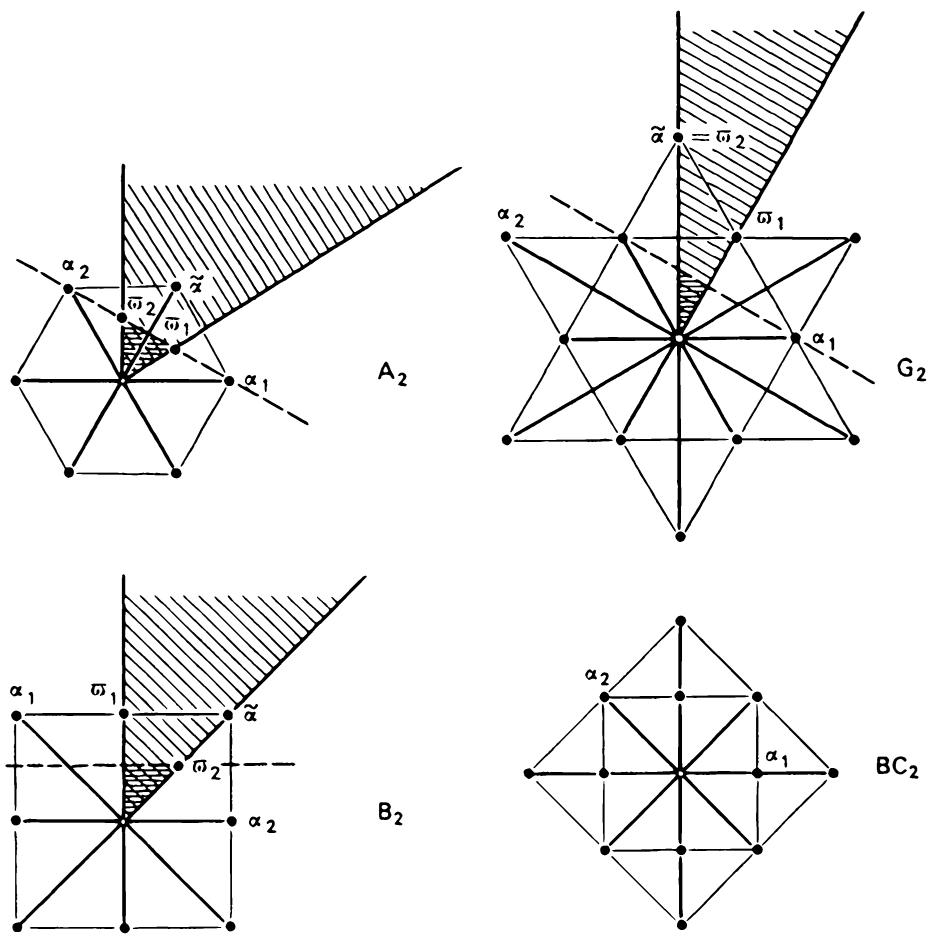
\includegraphics[keepaspectratio]{images/part002_e5dc67b9.jpg}}\\
上面的前三幅图表示 \(A_{2}\)、\(B_{2}\) 和 \(G_{2}\) 类型的根系 R。阴影区域表示与基 \((\alpha_{1},\alpha_{2})\) 相应的室 C。直线 \((x|\beta)=1\)，其中 \(\beta\) 表示

逆根系 \(R^{-}\) 的最高根；该直线以点线表示，双重阴影区域表示包含于 C 且顶点为 0 的 \(R^{-}\) 小室。

最后一幅图表示秩为 2 的唯一不可约非约化根系。

\specialchapter{根系的主要性质概述}

（在本概述中，我们限于约化根系的情形，并在实数域上工作。）

\begin{enumerate}
\def\labelenumi{\arabic{enumi})}
\tightlist
\item
  令 V 为实向量空间。V 中的约化根系是 V 的一个子集 R，具有以下性质：
\end{enumerate}

\begin{enumerate}
\def\labelenumi{(\roman{enumi})}
\item
  R 是有限集并且生成 V。
\item
  对所有 \(\alpha \in \mathbb{R}\)，存在 \(\alpha^{\vee} \in V^{*}\)，使得 \(\langle \alpha, \alpha^{\vee} \rangle = 2\)，并且使映射
\end{enumerate}

\[
s _ {\alpha}: x \mapsto x - \langle x, \alpha^{\vee} \rangle \alpha
\]

从 V 到 V 将 R 映到 R。

\begin{enumerate}
\def\labelenumi{(\roman{enumi})}
\setcounter{enumi}{2}
\item
  对所有 \(\alpha \in \mathbb{R}\)，有 \(\alpha^{\vee}(\mathbb{R}) \subseteq \mathbf{Z}\)。
\item
  若 \(\alpha \in \mathbb{R}\)，则 \(2\alpha \notin \mathbb{R}\)。
\end{enumerate}

鉴于 (i)，由 (ii) 保证存在的元素 \(\alpha^{\vee}\) 是唯一的；因此 (iii) 是有意义的。映射 \(s_{\alpha}\) 是一个反射，它固定 \(\mathrm{L}_{\alpha} = \mathrm{Ker}(\alpha^{\vee})\) 中的点，并将 \(\alpha\) 变为 \(-\alpha\)。

R 的元素称为根。V 的维数称为根系的秩。

\begin{enumerate}
\def\labelenumi{\arabic{enumi})}
\setcounter{enumi}{1}
\item
  保持 R 不变的 V 的自同构群记为 A(R)。\(s_{\alpha}\)（\(\alpha \in R\)）生成 A(R) 的一个子群 W(R)，称为 R 的 Weyl 群；该子群在 A(R) 中正规。属于 W(R) 的唯一反射是 \(s_{\alpha}\)。
\item
  集合 \(R^{-}\) 由 \(\alpha^{-}\)（其中 \(\alpha \in R\)）组成，是 \(V^{*}\) 中的一个约化根系，称为 R 的对偶根系。映射 \(\alpha \mapsto \alpha^{-}\) 是从 R 到 \(R^{-}\) 的一个双射，称为典范双射。我们有 \((\mathrm{R}^{-})^{-} = \mathrm{R}\)，并且典范双射 \(R \to R^{-}\) 和 \(R^{-} \to R\) 互为逆映射。映射 \(u \mapsto {}^{t}u^{-1}\) 给出从 \(W(R)\) 到 \(W(R^{-})\) 的一个同构；借助该同构，我们认同这两个群。
\item
  令 V 为实向量空间，并且是向量子空间 \(V_{1},\ldots,V_{r}\) 的直和。对每个 i，令 \(R_{i}\) 为 \(V_{i}\) 中的约化根系。则各 \(R_{i}\) 的并集 R 是 V 中的一个根系，称为各 \(R_{i}\) 的直和。群 \(W(R)\) 可认同为各 \(W(R_{i})\) 的直积。若 \(R \neq \varnothing\)，且 R 不是两个非空根系的直和，则称 R 是不可约的。这等价于说 \(W(R)\) 是不可约的。每个约化根系
\end{enumerate}

R 是不可约约化根系的直和；这些分支除排列外唯一确定，并称为 R 的不可约分支。

\begin{enumerate}
\def\labelenumi{\arabic{enumi})}
\setcounter{enumi}{4}
\item
  令 R 为 V 中的约化根系。V 上存在在 \(W(R)\) 作用下不变的标量积。下文用 \((x|y)\) 表示这样的标量积。若将 V 与 \(V^{*}\) 用 \((x|y)\) 认同，则有 \(\alpha^{\vee} = \frac{2\alpha}{(\alpha|\alpha)}\)。反射 \(s_{\alpha}\) 是将 \(\alpha\) 变为 \(-\alpha\) 的正交反射。若 R 不可约，则 Weyl 群在给定长度的根的集合上传递作用。若 R 不可约，则标量积 \((x|y)\) 除相差一个常数因子外是唯一的。
\item
  令 R 为一个约化根系。对 \(\alpha, \beta \in \mathbb{R}\)，置
\end{enumerate}

\[
\langle \alpha , \beta^{\vee} \rangle = n (\alpha , \beta) \in \mathbf {Z}.
\]

我们有

\[
\begin{array}{c} n (\alpha , \alpha) = 2, \\ s _ {\beta} (\alpha) = \alpha - n (\alpha , \beta) \beta , \\ n (\alpha , \beta) = \frac {2 (\alpha | \beta)}{(\beta | \beta)}. \end{array}
\]

除交换 \(\alpha\) 与 \(\beta\) 外，只有以下可能性：

\[
n (\alpha , \beta) = n (\beta , \alpha) = 0; \quad (\alpha , \beta) = \frac {\pi}{2}; \quad s _ {\alpha} s _ {\beta} \text {   of   order   } 2;
\]

\[
n (\alpha , \beta) = n (\beta , \alpha) = 1; \quad (\alpha , \beta) = \frac {\pi}{3}; \quad s _ {\alpha} s _ {\beta} \text {   of   order   } 3;
\]

\[
n (\alpha , \beta) = n (\beta , \alpha) = - 1; \quad (\alpha , \beta) = \frac {2 \pi}{3}; \quad s _ {\alpha} s _ {\beta} \text {   of   order   } 3;
\]

\[
n (\alpha , \beta) = 1, n (\beta , \alpha) = 2; \quad (\alpha , \beta) = \frac {\pi}{4}; \quad s _ {\alpha} s _ {\beta} \text {   of   order   } 4;
\]

\[
n (\alpha , \beta) = - 1, n (\beta , \alpha) = - 2; (\alpha , \beta) = \frac {3 \pi}{4}; s _ {\alpha} s _ {\beta} \text {   of   order   } 4;
\]

\[
n (\alpha , \beta) = 1, n (\beta , \alpha) = 3; \quad (\alpha , \beta) = \frac {\pi}{6}; \quad s _ {\alpha} s _ {\beta} \text {   of   order   } 6;
\]

\[
n (\alpha , \beta) = - 1, n (\beta , \alpha) = - 3; (\widehat {\alpha , \beta}) = \frac {5 \pi}{6}; s _ {\alpha} s _ {\beta} \text {   of   order   } 6;
\]

\[
n (\alpha , \beta) = n (\beta , \alpha) = 2; \quad \alpha = \beta ; \quad n (\alpha , \beta) = n (\beta , \alpha) = - 2; \quad \alpha = - \beta ;
\]
\[
\begin{gathered}
 n (\alpha , \beta) = n (\beta , \alpha) = 1 \Longrightarrow \| \alpha \| = \| \beta \| ; \quad n (\alpha , \beta) = n (\beta , \alpha) = -1 \Longrightarrow \| \alpha \| = \| \beta \| ; \\
 (n (\alpha , \beta) , n (\beta , \alpha)) = (1,2) \Longrightarrow \| \beta \| = \sqrt {2} \| \alpha \| ; \quad (n (\alpha , \beta) , n (\beta , \alpha)) = (-1,-2) \Longrightarrow \| \beta \| = \sqrt {2} \| \alpha \| ; \\
 (n (\alpha , \beta) , n (\beta , \alpha)) = (1,3) \Longrightarrow \| \beta \| = \sqrt {3} \| \alpha \| ; \quad (n (\alpha , \beta) , n (\beta , \alpha)) = (-1,-3) \Longrightarrow \| \beta \| = \sqrt {3} \| \alpha \| .
\end{gathered}
\]

\begin{enumerate}
\def\labelenumi{\arabic{enumi})}
\setcounter{enumi}{6}
\item
  令 \(\alpha, \beta \in \mathbb{R}\)。若 \((\alpha|\beta) > 0\)，则 \(\alpha + \beta\) 是一个根，除非 \(\alpha = \beta\)。若 \((\alpha|\beta) < 0\)，则 \(\alpha + \beta\) 是一个根，除非 \(\alpha = -\beta\)。
\item
  令 \(\alpha, \beta\) 为两个不成比例的根。集合 I 由 \(j \in \mathbf{Z}\) 组成；其中 \(\beta + j\alpha \in \mathbb{R}\) 成立。它是包含 0 的、记为 \([-q, p]\) 的 \(\mathbf{Z}\) 区间。我们有
\end{enumerate}

\[
p - q = - n (\beta , \alpha), \quad \frac {q + 1}{p} = \frac {(\beta + \alpha | \beta + \alpha)}{(\beta | \beta)}.
\]

令 S 为 \(\beta + j\alpha\)（\(j \in I\)）所成的集合。则 \(s_{\alpha}(S) = S\) 且 \(s_{\alpha}(\beta + p\alpha) = \beta - q\alpha\)。我们称 S 为 \(\alpha\)-根链，它由 \(\beta\) 定义；称 \(\beta - q\alpha\) 为其起点，称 \(\beta + p\alpha\) 为其终点，并称 \(p + q\) 为其长度。

若 T 是 \(\alpha\)-根链，起点为 \(\gamma\)，则 T 的长度为 \(-n(\gamma, \alpha)\)。

\begin{enumerate}
\def\labelenumi{\arabic{enumi})}
\setcounter{enumi}{8}
\item
  令 X 为 \(\operatorname{Ker}\alpha^{\vee}\)（\(\alpha\in R\)）的并集。V-X 的连通分支称为 R 在 V 中的室。它们是开单纯锥。Weyl 群在室的集合上单传递地作用。若 C 是一个室，则 \(\overline{C}\) 是 \(\mathrm{W}(\mathrm{R})\) 的基本域。我们有 \((x|y)>0\) 对 \(x,y\in C\) 成立。由从 V 到 \(V^{*}\)、与 \((x|y)\) 对应的双射，将 V 中 R 的室集合双射到 \(R^{\vee}\) 中 \(V^{*}\) 的室集合；我们把 \(C^{\vee}\) 记为 C 在此双射下的像。
\item
  令 C 为 R 的一个室。令 \(L_{1}, L_{2}, \ldots, L_{l}\) 为 C 的壁。对每个 i，存在唯一的根 \(\alpha_{i}\)，使得 \(L_{i} = L_{\alpha_{i}}\)，且 \(\alpha_{i}\) 与 \(L_{i}\) 位于同一侧。族 \((\alpha_{1}, \ldots, \alpha_{l})\) 是 V 的一个基，而 C 是 \(x \in V\) 中满足对所有 i 有 \(\langle \alpha_{i}, x \rangle > 0\) 的元素所成的集合，换言之，是满足对所有 i 有 \((\alpha_{i} | x) > 0\) 的集合。于是 \(\{\alpha_{1}, \ldots, \alpha_{l}\}\) 称为由 C 定义的 R 的基 B(C)。我们有 \((\alpha_{i} | \alpha_{j}) \leqslant 0\)；当 \(i \neq j\) 时。Weyl 群在基的集合上单传递地作用。每个根都可由 W(R) 的某个元素变换为 B(C) 中的一个元素。我们有 \(\{\alpha_{1}^{\vee}, \ldots, \alpha_{l}^{\vee}\} = B(C^{\vee})\)。
\item
  置 \(s_{\alpha_i} = s_i\)，令 \(S\) 为各 \(s_i\) 所成的集合，并令 \(m_{ij}\) 为 \(s_i s_j\) 的阶。对 (W(R), S) 而言，这是带有 Coxeter 矩阵（\(m_{ij}\)）的 Coxeter 系统；换言之，W(R) 由生成元（\(s_i\)）\(_{1 \leqslant i \leqslant l}\) 及关系（\(s_i s_j\)）\(^{m_{ij}} = 1\) 定义。W(R) 中的两个元素 \(s_i\) 和 \(s_j\) 共轭，当且仅当存在指标序列（\(i_1, i_2, \ldots, i_q\)），使得 \(i_1 = i, i_q = j\)，并且每个 \(m_{i_l i_{l+1}}\) 都等于 3。
\item
  令 \(n_{ij} = n(\alpha_i, \alpha_j)\)。矩阵 \((n_{ij})_{1 \leqslant i,j \leqslant l}\) 称为 \(R\) 的 Cartan 矩阵。它（除 \(1, 2, \ldots, l\) 的排列外）与 \(C\) 的选择无关。我们有 \(n_{ii} = 2\)。\(n_{ij} \in \{0, -1, -2, -3\}\) 对 \(i \neq j\) 成立。如果两个根系具有相同的 Cartan 矩阵，则它们同构。
\item
  令 \(G\) 为 \(A(R)\) 中保持 \(B(C)\) 不变的子群。则 \(A(R)\) 是 \(G\) 与 \(W(R)\) 的半直积。
\item
  由 C 在 V（分别为 \(V^{*}\)）上定义的序关系，是与 V（分别为 \(V^{*}\)）的向量空间结构相容的序关系；其中 \(\geqslant 0\) 的元素是 \(\alpha_{i}\)（分别为 \(\alpha_{i}^{\vee}\)）的系数为 \(\geqslant 0\) 的线性组合。这些元素称为关于 C 或 B(C) 的正元素。这些序关系也由 \(C^{\vee}\) 定义。V 的一个元素为 \(\geqslant 0\)，当且仅当它在 \(C^{\vee}\) 上的取值为 \(\geqslant 0\)。关于 C 的 \(\geqslant 0\) 元素集合包含 \(\overline{C}\)，但一般不同于 \(\overline{C}\)。令 \(x \in V\)。则 \(x \in \overline{C}\) 当且仅当 \(x \geqslant w(x)\) 对所有 \(w \in W(R)\) 都成立；而 \(x \in C\) 当且仅当 \(x > w(x)\) 对所有不同于 1 的 \(w \in W(R)\) 都成立。
\item
  每个根对于 \(C\) 不是正的就是负的。我们把 \(R_{+}(C)\) 记为对于 \(C\) 为正的根所成的集合，于是 \(R = R_{+}(C) \cup (-R_{+}(C))\) 是 R 的一个划分。反射 \(s_{i}\) 将 \(\alpha_{i}\) 变为 \(-\alpha_{i}\)，并将 \(\mathrm{R}_{+}(\mathrm{C})\) 中异于 \(\alpha_{i}\) 的元素彼此置换。
\item
  设 B 是 R 的一个基。对于 B 为正的（分别为负的）每个根，都是 B 中元素的线性组合，其系数全为整数 \(\geqslant 0\)（分别为 \(\leqslant 0\)）。
\item
  设 \((\beta_{1},\beta_{2},\ldots,\beta_{n})\) 是一列对于 C 为正的根，并且 \(\beta_{1}+\cdots+\beta_{n}\) 是一个根。存在一个置换 \(\pi\in S_{n}\)，使得对所有 \(i\in\{1,2,\ldots,n\}\)，\(\beta_{\pi(1)}+\beta_{\pi(2)}+\cdots+\beta_{\pi(i)}\) 都是一个根。
\item
  设 \(\alpha \in \mathrm{R}_{+}(\mathrm{C})\)。则 \(\alpha \in \mathrm{B}(\mathrm{C})\)，当且仅当 \(\alpha\) 不能写成正根之和。
\item
  设 C 为一个室，\((\alpha_{1},\alpha_{2},\ldots,\alpha_{l})\) 为相应的基。对 \(I=\{1,2,\ldots,l\}\) 的任意子集 J，令 \(W_{J}\) 为 \(W(R)\) 的由 \(s_{i}\)（满足 \(i\in J\)）生成的子群。令 \(C_{J}\) 为 \(\alpha_{j}\)（\(j\in J\)）的系数为 \textgreater0 的线性组合所成的集合，于是 \(C_{J}\) 是 C 的一个面。
\end{enumerate}

令 \(J \subset I\)，\(g \in W(R)\)。以下条件等价：

\begin{enumerate}
\def\labelenumi{\alph{enumi})}
\item
  g 使 \(C_{J}\) 中的某一点不变：
\item
  g 使 \(C_{J}\) 中的每一点不变；
\item
  \(g\) 使 \(\overline{\mathbf{C}_{\mathrm{J}}}\) 中的每一点不变；
\end{enumerate}

\(d) g(C_{J}) = C_{J};\)

\begin{enumerate}
\def\labelenumi{\alph{enumi})}
\setcounter{enumi}{4}
\tightlist
\item
  \(g(\overline{\mathrm{C}_{\mathrm{J}}}) = \overline{\mathrm{C}_{\mathrm{J}}}\) ;
\end{enumerate}

\(f) g \in W_{J}\) .

令 \(J, J' \subset \{1, 2, \ldots, l\}\)，且 \(g, g' \in W(R)\)。以下条件等价：

\begin{enumerate}
\def\labelenumi{\alph{enumi})}
\item
  \(g(\mathrm{C}_{\mathrm{J}}) = g'(\mathrm{C}_{\mathrm{J}'})\) ;
\item
  \(g(\mathrm{C}_{\mathrm{J}})\cap g'(\mathrm{C}_{\mathrm{J}'})\neq \emptyset ;\)
\item
  \(g\mathrm{W}_{\mathrm{J}} = g^{\prime}\mathrm{W}_{\mathrm{J}^{\prime}}\)
\end{enumerate}

\(d) J = J' \text{ 且 } g' \in gW_J.\)

令 \(J_1, J_2, \ldots, J_r \subset I\)，且 \(J = J_1 \cap \cdots \cap J_r\)。则 \(W_J = W_{J_1} \cap \cdots \cap W_{J_r}\)。对所有 \(g \in W(R)\)，存在 \(J \subset I\)，使得 \(\overline{C} \cap g(\overline{C}) = \overline{C}_J\) 且 \(g \in W_J\)。

\begin{enumerate}
\def\labelenumi{\arabic{enumi})}
\setcounter{enumi}{19}
\tightlist
\item
  令 \(\mathbf{P}\) 为 \(\mathbb{R}\) 的一个子集。称 \(\mathbf{P}\) 为闭的，是指条件 \(\alpha \in \mathbb{P}, \beta \in \mathbb{P}, \alpha + \beta \in \mathbb{R}\) 蕴含 \(\alpha + \beta \in \mathbb{P}\)；称 \(\mathbf{P}\) 为抛物的，是指 \(\mathbf{P}\) 闭且满足 \(\mathbf{P} \cup (-\mathbf{P}) = \mathbb{R}\)。以下条件等价：
\end{enumerate}

\begin{enumerate}
\def\labelenumi{\alph{enumi})}
\item
  P 是抛物集；
\item
  P 是闭集，并且存在一个室 C，使得 \(P \supset R_{+}(C)\)；
\item
  存在一个室 C 和 B(C) 的一个子集 \(\Sigma\)，使得 P 是 \(R_{+}(C)\) 与根的集合 Q 的并集，其中 Q 由 \(\Sigma\) 中元素的系数为整数 \(\leqslant 0\) 的线性组合组成。
\end{enumerate}

假设这些条件成立，并令 \(V_{1}\) 为 V 中由 \(\Sigma\) 生成的向量子空间。则

\[
P \cap (- P) = Q \cup (- Q) = V _ {1} \cap R,
\]

且 \(P \cap (-P)\) 是 \(V_1\) 中以 \(\Sigma\) 为基的根系。

令 \(P', C', \Sigma'\) 具有相应的性质。若存在 \(W(R)\) 的一个元素将 P 变为 \(P'\)，则存在 \(W(R)\) 的一个元素，将 C 变为 \(C'\)，将 \(\Sigma\) 变为 \(\Sigma'\)，并将 P 变为 \(P'\)。

\begin{enumerate}
\def\labelenumi{\arabic{enumi})}
\setcounter{enumi}{20}
\tightlist
\item
  令 \(\mathbf{P}\) 为 \(\mathbb{R}\) 的一个子集。以下条件等价：
\end{enumerate}

\begin{enumerate}
\def\labelenumi{\alph{enumi})}
\item
  存在一个室 C，使得 \(P = R_{+}(C)\)：
\item
  P 是闭集，且 \(\{P, -P\}\) 是 R 的一个划分。
\end{enumerate}

此时室 C 是唯一的。

假设 V 配备了有序向量空间的结构，使得每个根或者为正或者为负。令 \(R_{+}\) 为关于此结构的正根所成的集合。存在唯一的室 C，使得 \(\mathrm{R}_{+} = \mathrm{R}_{+}(\mathrm{C})\)。

\begin{enumerate}
\def\labelenumi{\arabic{enumi})}
\setcounter{enumi}{21}
\item
  R 的子集 B 是 R 的一个基，当且仅当 B 中的元素线性无关，并且每个根都是 B 中元素的线性组合，且其系数要么全为 \(\geqslant 0\)，要么全为 \(\leqslant 0\)。
\item
  令 \(\mathbf{P}\) 为 \(\mathbf{R}\) 的一个闭子集，并满足 \(\mathbf{P} \cap (-\mathbf{P}) = \varnothing\)。存在一个室 \(\mathbf{C}\)，使得 \(\mathbf{P} \subset R_{+}(\mathbf{C})\)。
\item
  若 P = -P，则称 R 的子集 P 为对称的。令 P 为 R 的一个子集，并令 \(V_{1}\)（分别为 \(\Gamma\)）为 V 中由 P 生成的向量子空间（分别为加法子群）。以下条件等价：
\end{enumerate}

\begin{enumerate}
\def\labelenumi{\alph{enumi})}
\item
  P 是闭的且对称的；
\item
  P 是闭的，并且是 \(V_{1}\) 中的一个根系；
\item
  \(\Gamma \cap \mathbb{R} = \mathbb{P}\) .
\end{enumerate}

\begin{enumerate}
\def\labelenumi{\arabic{enumi})}
\setcounter{enumi}{24}
\tightlist
\item
  假设 R 不可约。令 C 为一个室，置
\end{enumerate}

\[
\mathrm{B} (\mathrm{C}) = \left\{\alpha_ {1}, \dots , \alpha_ {l} \right\}.
\]

R 中存在最高元素（相对于 C 所定义的序），即存在 R 的一个元素 \(\tilde{\alpha}=n_{1}\alpha_{1}+\cdots+n_{l}\alpha_{l}\)，使得对于任意根

\[
p _ {1} \alpha_{1} + \dots + p _ {l} \alpha_{l}.
\]

\(n_1 \geqslant p_1, \ldots, n_l \geqslant p_l\)。于是 \(\tilde{\alpha} \in \overline{C}\)，并且有 \(\| \tilde{\alpha} \| \geqslant \| \alpha \|\)（对每个根 \(\alpha\)）。

\begin{enumerate}
\def\labelenumi{\arabic{enumi})}
\setcounter{enumi}{25}
\tightlist
\item
  V 中由 R 生成的子群记为 Q(R)；Q(R) 的元素称为 R 的根权。群 Q(R) 是 V 中秩为 \(l = \dim V\) 的离散子群。R 的任一基都是 Q(R) 的一个基。
\end{enumerate}

与 \(Q(R^{\vee})\) 对应的 V 的子群记为 \(P(R)\)；\(P(R)\) 的元素称为 R 的权。群 \(P(R)\) 是 V 中秩为 l、包含 \(Q(R)\) 的离散子群。群 \(P(R)/Q(R)\)、\(P(R^{\vee})/Q(R^{\vee})\) 是有限群且彼此同构；它们的阶 f 称为 R 的连接指标。按 25) 的记号，\(W(R)\) 的阶为 \(l!n_{1}n_{2}\ldots n_{l}f\)。

群 \(A(R)\) 保持 \(P(R)\)、\(Q(R)\) 不变，因而作用于 \(P(R)/Q(R)\)。群 \(W(R)\) 在 \(P(R)/Q(R)\) 上作用平凡，所以 \(A(R)/W(R)\) 作用于 \(P(R)/Q(R)\)。

\begin{enumerate}
\def\labelenumi{\arabic{enumi})}
\setcounter{enumi}{26}
\tightlist
\item
  令 C 为一个室。令 \(B = (\alpha_{1}, \ldots, \alpha_{l})\) 为相应的 R 的基。对偶基 \((\omega_{1}, \ldots, \omega_{l})\)（相对于 \((\alpha_{1}^{\vee}, \ldots, \alpha_{l}^{\vee})\)）是 P(R) 的一个基。称 \(\omega_{i}\) 为基本权（关于 C 或关于 B）。\(\omega_{i}\) 的系数为 \textgreater{} 0（分别为 \(\geqslant 0\)）的线性组合所成的集合是 C（分别是 \(\overline{C}\)）。\(\omega_{i}\) 的系数为整数 \(\geqslant 0\) 的线性组合称为支配权。P(R) 的每个元素都可由 W(R) 的某个元素变换为唯一的支配权。支配权正是 V 中的元素 \(\omega\)，它满足 \(\frac{2(\omega|\alpha_{i})}{(\alpha_{i}|\alpha_{i})}\) 是一个 \(\geqslant 0\) 的整数。
\end{enumerate}

\[
28) \text {   Let   } \rho = \frac {1}{2} \sum_ {\alpha \in R _ {+} (C)} \alpha . \text {   Then,   } \rho = \omega_ {1} + \dots + \omega_ {l} \in C.
\]

\begin{enumerate}
\def\labelenumi{\arabic{enumi})}
\setcounter{enumi}{28}
\item
  令 \(\mathbf{T}\) 为 \(\mathbf{V}^*\) 的平移群，其向量属于 \(\mathrm{Q}(\mathbb{R}^{\vee})\)。\(\mathbf{V}^*\) 的仿射变换群由 \(\mathbf{T}\) 和 \(\mathrm{W}(\mathbb{R})\) 生成，是 \(\mathrm{W}(\mathbb{R})\) 与 \(\mathbf{T}\) 的半直积。该群称为 \(\mathbb{R}\) 的仿射 Weyl 群，记为 \(\mathrm{W}_a(\mathbb{R})\)。它在 \(\mathbf{V}^*\) 上适当作用。对 \(\alpha \in \mathbb{R}\) 和 \(\lambda \in \mathbf{Z}\)，令 \(s_{\alpha, \lambda}\) 为映射 \(x^* \mapsto x^* - \langle x^*, \alpha \rangle \alpha^{\vee} + \lambda \alpha^{\vee}\)；这是一个仿射反射，而其不动点集 \(L_{\alpha, \lambda}\) 由方程 \(\langle x^*, \alpha \rangle = \lambda\) 定义；我们有 \(L_{\alpha, \lambda} = L_{\alpha} + \frac{1}{2}\lambda \alpha^{\vee}\)。\(s_{\alpha, \lambda}\) 是属于 \(W_a(\mathbb{R})\) 的仿射反射，并且它们生成群 \(W_a(\mathbb{R})\)。
\item
  令 \(\mathbf{E}\) 为各 \(L_{\alpha, \lambda}\) 的并集，其中 \(\alpha \in \mathbb{R}\) 且 \(\lambda \in \mathbf{Z}\)。\(V^{*} - E\) 的连通分支称为 \(\mathbb{R}\) 的小室。若 \(\mathbb{R}\) 不可约，则每个小室都是开单纯形；一般地，小室是开单纯形的乘积。群 \(W_{a}(\mathbb{R})\) 在小室的集合上单传递地作用。若 \(\mathbb{C}\) 是一个小室，则 \(\overline{\mathbb{C}}\) 是 \(W_{a}(\mathbb{R})\) 的基本域。令 \(\sigma_{1}, \ldots, \sigma_{q}\) 为 \(W_{a}(\mathbb{R})\) 中与 \(\mathbb{C}\) 的壁对应的反射；令 \(\mu_{ij}\) 为 \(\sigma_{i}\sigma_{j}\) 的阶。则 \(W_{a}(\mathbb{R})\) 由生成元 \(\sigma_{i}\) 及关系 \((\sigma_{i}\sigma_{j})^{\mu_{ij}} = 1\) 定义。
\item
  若 \(p \in \mathrm{P}(\mathbb{R}^{\vee})\)，则存在一个小室 \(C\)，使得 \(p\) 是 \(\overline{\mathbb{C}}\) 的一个极点。若 \(\mathbf{C}'\) 是一个小室，则存在唯一的根权，它是 \(\overline{\mathbb{C}'}\) 的一个极点。
\end{enumerate}

令 \(x^{*} \in V^{*}\)；以下条件等价：

\begin{enumerate}
\def\labelenumi{\alph{enumi})}
\item
  \(x^{*} \in \mathrm{P}(\mathrm{R}^{\vee})\) ;
\item
  对所有 \(\alpha \in \mathbb{R}\)，与 \(\mathbf{L}_{\alpha}\) 平行且经过 \(x^{*}\) 的超平面是 \(\mathbf{L}_{\alpha,\lambda}\) 中的一个。
\end{enumerate}

令 \(C'\) 为 \(R^{\vee}\) 的一个室。存在唯一的小室 \(C\) 包含于 \(C'\) 中，并满足 \(0 \in \overline{C}\)。假设 \(R\) 不可约，并令 \(\beta\) 为 \(R\) 的最高根（关于 \(C'\)）；则 \(C\) 是 \(x^{*} \in C'\) 中满足 \(\langle x^{*}, \beta \rangle < 1\) 的元素所成的集合。

\begin{enumerate}
\def\labelenumi{\arabic{enumi})}
\setcounter{enumi}{31}
\item
  令 S 为 V 的对称代数。\(S^{W}\) 是由在 \(W = W(R)\) 下不变的元素组成的子代数，g 为 W 的阶。\(l = \dim V\)。存在齐次的、代数独立的元素 \(I_{1}, I_{2}, \ldots, I_{l}\)，它们生成 \(S^{W}\)。S 作为 \(S^{W}\)-模有一个由 g 个齐次元素组成的基。令 a 为 S 中由 \(S^{W}\) 的次数 \textgreater0 的齐次元素生成的理想：W 在 S/a 上的表示，是 W 在 S 上的表示通过取商所诱导的表示，同构于 W 的正则表示（在 R 上）。
\item
  令 \(I_1, I_2, \ldots, I_l\) 为生成 \(S^W\) 的齐次代数独立元素。其次数 \(k_1, k_2, \ldots, k_l\) 由 \(R\) 唯一确定（除排列外）。我们有 \(g = k_1k_2\ldots k_l\)。根的数目为 \(2\sum_{i=1}^{l}(k_i - 1)\)。
\item
  S 中的元素 A 若满足 \(w(A) = \det(w)\) 对所有 \(w \in W\) 成立，则称其在 W 下反不变。令 \(R = R_{1} \cup (-R_{1})\) 为 R 的一个划分，并置 \(\pi = \prod_{\alpha \in R_{1}} \alpha\)。S 中的元素 \(\pi\) 是反不变的：S 的反不变元素正是 \(\pi I\) 的形式，其中 \(I \in S^{W}\)。
\item
  令 E 为 R 的权群 P 的群代数 Z[P]。若 \(p \in P\)，我们用 \(e^{p}\) 表示 E 中相应的元素。我们有 \(e^{p}e^{p'} = e^{p+p'}\)，并且 \(e^{p}\) 构成 E 的一个基。W 在 E 上有一个作用，使得 \(w(e^{p}) = e^{w(p)}\) 在 \(w \in W\) 且 \(p \in P\) 时成立。若 E 中的元素 \(z \in E\) 满足 \(w(z) = \det(w).z\) 对所有 \(w \in W\) 成立，则称其为反不变元素。对所有 \(z \in E\)，置 \(J(z) = \sum_{w \in W} \det(w).w(z)\)。令 C 为一个室。\(J(e^{p})\)（其中 \(p \in P \cap C\)）构成 E 的反不变元素群的一个基。若 \(\rho\) 是正根之和的一半，则有：
\end{enumerate}

\[
J \left(e ^ {\rho}\right) = e ^ {\rho} \prod_ {\alpha > 0} \left(1 - e ^ {- \alpha}\right) = \prod_ {\alpha > 0} \left(e ^ {\alpha / 2} - e ^ {- \alpha / 2}\right),
\]

这些乘积是对根 \textgreater{} 0 的集合取的。

\begin{enumerate}
\def\labelenumi{\arabic{enumi})}
\setcounter{enumi}{35}
\tightlist
\item
按 35) 的记号，置
\end{enumerate}

\[
z _ {p} = \mathrm{J} (e ^ {p + \rho}) / \mathrm{J} (e ^ {\rho}) \quad \text { for } p \in \mathrm{P}.
\]

\(z_{p}\)（其中 \(p \in \mathrm{P} \cap \overline{\mathrm{C}}\)）构成由 W 不变的 E 中元素组成的群 \(\mathbf{E}^{\mathbf{W}}\) 的一个基。若 \(\omega_{1}, \ldots, \omega_{l}\) 是 R 的基本权，则元素 \(z_{\omega_{i}}\)（\(1 \leqslant i \leqslant l\)）代数独立并生成环 \(\mathbf{E}^{\mathbf{W}}\)。

\begin{enumerate}
\def\labelenumi{\arabic{enumi})}
\setcounter{enumi}{36}
\tightlist
\item
  令 C 为 R 的一个室，\((\alpha_{1},\ldots,\alpha_{l})\) 为相应的基。W 中的元素 \(c=s_{1}s_{2}\ldots s_{l}\) 称为 R 的 Coxeter 变换。c 的共轭类不依赖于 C 或 \(\alpha_{i}\) 的编号。c 的阶 h 称为 R 的 Coxeter 数。c 的特征值形如 \(\exp\frac{2i\pi m_{j}}{h}\)，其中整数 \(m_{1},m_{2},\ldots,m_{l}\)（称为 R 的指数）满足 \(1\leqslant m_{1}\leqslant m_{2}\leqslant\cdots\leqslant m_{l}\leqslant h-1\)。
\end{enumerate}

假设 R 不可约。则

\[
m _ {1} = 1, m _ {l} = h - 1.
\]

\[
m _ {j} + m _ {l + 1 - j} = h \quad (1 \leqslant j \leqslant l).
\]

\[
m _ {1} + m _ {2} + \dots + m _ {l} = \frac {1}{2} l h = \frac {1}{2} \operatorname{Card} (\mathrm{R}).
\]

每个与 h 互素的 \(m \in \{1, 2, \ldots, h - 1\}\) 恰好等于某一个 \(m_j\)。数 \(m_1 + 1, m_2 + 1, \ldots, m_l + 1\) 与 33) 中记为 \(k_1, k_2, \ldots, k_l\) 的整数重合（除排列外）。按 25) 的记号，\(n_1 + \cdots + n_l = h - 1\)。在 R 上，\(\{1, c, c^2, \ldots, c^{h-1}\}\) 有 l 个轨道，每个轨道含有 h 个元素。

若 \(h\) 为偶数，则 \(c^{h/2}\) 将 \(C\) 变为 \(-C\)。我们有 \(-1 \in W\)，当且仅当 \(W\) 的指数全为奇数；在这种情况下，\(h\) 为偶数且 \(c^{h/2} = -1\)。

\pandocbounded{
\includegraphics[keepaspectratio]{images/part002_b04bf376.jpg}}

\end{document}
